\documentclass[twoside]{book}

% Packages required by doxygen
\usepackage{fixltx2e}
\usepackage{calc}
\usepackage{doxygen}
\usepackage[export]{adjustbox} % also loads graphicx
\usepackage{graphicx}
\usepackage[utf8]{inputenc}
\usepackage{makeidx}
\usepackage{multicol}
\usepackage{multirow}
\PassOptionsToPackage{warn}{textcomp}
\usepackage{textcomp}
\usepackage[nointegrals]{wasysym}
\usepackage[table]{xcolor}

% Font selection
\usepackage[T1]{fontenc}
\usepackage[scaled=.90]{helvet}
\usepackage{courier}
\usepackage{amssymb}
\usepackage{sectsty}
\renewcommand{\familydefault}{\sfdefault}
\allsectionsfont{%
  \fontseries{bc}\selectfont%
  \color{darkgray}%
}
\renewcommand{\DoxyLabelFont}{%
  \fontseries{bc}\selectfont%
  \color{darkgray}%
}
\newcommand{\+}{\discretionary{\mbox{\scriptsize$\hookleftarrow$}}{}{}}

% Page & text layout
\usepackage{geometry}
\geometry{%
  a4paper,%
  top=2.5cm,%
  bottom=2.5cm,%
  left=2.5cm,%
  right=2.5cm%
}
\tolerance=750
\hfuzz=15pt
\hbadness=750
\setlength{\emergencystretch}{15pt}
\setlength{\parindent}{0cm}
\setlength{\parskip}{3ex plus 2ex minus 2ex}
\makeatletter
\renewcommand{\paragraph}{%
  \@startsection{paragraph}{4}{0ex}{-1.0ex}{1.0ex}{%
    \normalfont\normalsize\bfseries\SS@parafont%
  }%
}
\renewcommand{\subparagraph}{%
  \@startsection{subparagraph}{5}{0ex}{-1.0ex}{1.0ex}{%
    \normalfont\normalsize\bfseries\SS@subparafont%
  }%
}
\makeatother

% Headers & footers
\usepackage{fancyhdr}
\pagestyle{fancyplain}
\fancyhead[LE]{\fancyplain{}{\bfseries\thepage}}
\fancyhead[CE]{\fancyplain{}{}}
\fancyhead[RE]{\fancyplain{}{\bfseries\leftmark}}
\fancyhead[LO]{\fancyplain{}{\bfseries\rightmark}}
\fancyhead[CO]{\fancyplain{}{}}
\fancyhead[RO]{\fancyplain{}{\bfseries\thepage}}
\fancyfoot[LE]{\fancyplain{}{}}
\fancyfoot[CE]{\fancyplain{}{}}
\fancyfoot[RE]{\fancyplain{}{\bfseries\scriptsize Generated by Doxygen }}
\fancyfoot[LO]{\fancyplain{}{\bfseries\scriptsize Generated by Doxygen }}
\fancyfoot[CO]{\fancyplain{}{}}
\fancyfoot[RO]{\fancyplain{}{}}
\renewcommand{\footrulewidth}{0.4pt}
\renewcommand{\chaptermark}[1]{%
  \markboth{#1}{}%
}
\renewcommand{\sectionmark}[1]{%
  \markright{\thesection\ #1}%
}

% Indices & bibliography
\usepackage{natbib}
\usepackage[titles]{tocloft}
\setcounter{tocdepth}{3}
\setcounter{secnumdepth}{5}
\makeindex

% Hyperlinks (required, but should be loaded last)
\usepackage{ifpdf}
\ifpdf
  \usepackage[pdftex,pagebackref=true]{hyperref}
\else
  \usepackage[ps2pdf,pagebackref=true]{hyperref}
\fi
\hypersetup{%
  colorlinks=true,%
  linkcolor=blue,%
  citecolor=blue,%
  unicode%
}

% Custom commands
\newcommand{\clearemptydoublepage}{%
  \newpage{\pagestyle{empty}\cleardoublepage}%
}

\usepackage{caption}
\captionsetup{labelsep=space,justification=centering,font={bf},singlelinecheck=off,skip=4pt,position=top}

%===== C O N T E N T S =====

\begin{document}

% Titlepage & ToC
\hypersetup{pageanchor=false,
             bookmarksnumbered=true,
             pdfencoding=unicode
            }
\pagenumbering{alph}
\begin{titlepage}
\vspace*{7cm}
\begin{center}%
{\Large H\+ArD\+:\+:Core3D }\\
\vspace*{1cm}
{\large Generated by Doxygen 1.8.13}\\
\end{center}
\end{titlepage}
\clearemptydoublepage
\pagenumbering{roman}
\tableofcontents
\clearemptydoublepage
\pagenumbering{arabic}
\hypersetup{pageanchor=true}

%--- Begin generated contents ---
\chapter{Main Page}
\label{index}\hypertarget{index}{}H\+Ar\+D\+::\+Core (sources\+: \href{https://github.com/jdroniou/HArDCore}{\texttt{ https\+://github.\+com/jdroniou/\+H\+Ar\+D\+Core}}) provides a suite of C++ tools to implement numerical schemes whose unknowns are polynomials in the cells, on the edges, and on the faces. The focus is on dealing on generic polytopal meshes. This documentation addresses the 3D version of H\+Ar\+D\+::\+Core, but similar principles are valid for the 2D version. Transferring a scheme\textquotesingle{}s implementation from 3D to 2D or vice-\/versa is very straightforward, provided that the scheme\textquotesingle{}s mathematical definition does not depend on the dimension and that the generic types provided in {\ttfamily \mbox{\hyperlink{basis_8hpp_source}{basis.\+hpp}}} are used; see readme file of the H\+Ar\+D\+::\+Core github depository \href{https://github.com/jdroniou/HArDCore}{\texttt{ https\+://github.\+com/jdroniou/\+H\+Ar\+D\+Core}}.

\label{_build}%
 \hypertarget{index_build}{}\doxysection{Build instructions}\label{index_build}
\hypertarget{index_buildlib}{}\doxysubsection{Building the libraries and the schemes}\label{index_buildlib}
To build the libraries and implemented schemes, the minimal requirements are\+:


\begin{DoxyItemize}
\item C\+Make version 2.\+6 or above (\href{https://cmake.org/}{\texttt{ https\+://cmake.\+org/}})
\item A C++ compiler that supports the C++14 standard, eg. G\+CC (\href{https://gcc.gnu.org/}{\texttt{ https\+://gcc.\+gnu.\+org/}}) or Clang (\href{https://clang.llvm.org/}{\texttt{ https\+://clang.\+llvm.\+org/}})
\item Eigen C++ library, version 3.\+3 or above (\href{http://eigen.tuxfamily.org/}{\texttt{ http\+://eigen.\+tuxfamily.\+org/}})
\item The following Boost C++ libraries (\href{http://www.boost.org/}{\texttt{ http\+://www.\+boost.\+org/}})\+: filesystem, program options, timer, chrono.
\end{DoxyItemize}

Make sure that you have the development version of boost installed. On Linux, install {\ttfamily libboost-\/dev}, {\ttfamily libboost-\/filesystem-\/dev}, {\ttfamily libboost-\/program-\/options-\/dev}, {\ttfamily libboost-\/chrono-\/dev} and {\ttfamily libboost-\/timer-\/dev} from your package manager.

The linear systems resulting from the assembled scheme are solved using the Bi\+C\+G\+Stab implementation of Eigen. Alternatives are also provided, but require additional libraries (U\+M\+F\+P\+A\+CK, S\+U\+P\+E\+R\+LU, etc.); see the main C\+Make\+Lists.\+txt file.

Once you have installed all of the required dependencies, set up the build directory and generate the build files by running the following from the repository root\+:


\begin{DoxyCode}{0}
\DoxyCodeLine{mkdir build}
\DoxyCodeLine{cd build}
\DoxyCodeLine{cmake ..}
\DoxyCodeLine{make}
\end{DoxyCode}


After this, {\ttfamily build/\+Schemes} will contain the executables (e.\+g. {\ttfamily hho-\/diffusion}) to run the schemes. These executables need to access the typ2 meshes, which they should naturally find if you put the {\ttfamily typ2\+\_\+meshes} directory at the root of the project\textquotesingle{}s files.\hypertarget{index_doco}{}\doxysubsection{Building the Documentation}\label{index_doco}
The mesh documentation is built with Doxygen (\href{http://www.stack.nl/~dimitri/doxygen/}{\texttt{ http\+://www.\+stack.\+nl/$\sim$dimitri/doxygen/}}). If you are reading this then somebody has already built it for you. If you modify the code and wish to rebuild the documentation, simply run {\ttfamily doxygen} from the root directory. The H\+T\+ML version of the documentation is generated inside {\ttfamily documentation/html} and the La\+TeX version is generated inside {\ttfamily documentation/latex} and can be compiled using the generated Makefile.

\label{_mesh}%
 \hypertarget{index_mesh}{}\doxysection{Mesh module}\label{index_mesh}
\hypertarget{index_meshpple}{}\doxysubsection{Principles}\label{index_meshpple}
After it is loaded, the mesh is represented by classes describing a vertex, an edge, a face, and a cell\+: \mbox{\hyperlink{classHArDCore3D_1_1Vertex}{Vertex}}, \mbox{\hyperlink{classHArDCore3D_1_1Edge}{Edge}}, \mbox{\hyperlink{classHArDCore3D_1_1Face}{Face}}, and \mbox{\hyperlink{classHArDCore3D_1_1Cell}{Cell}}. Each of these classes contains methods to access useful information for the corresponding element, including other geometrical quantities it is related to. The mesh itself is represented by an element of the \mbox{\hyperlink{classHArDCore3D_1_1Mesh}{Mesh}} class with methods to access all the vertices, edges, faces and cells (or a particular vertex, edge, face or cell).

For example, if {\ttfamily mesh\+\_\+ptr} is a pointer to a Mesh class, the lines 
\begin{DoxyCode}{0}
\DoxyCodeLine{Vertex* vertex = mesh\_ptr-\/>vertex(5);}
\DoxyCodeLine{}
\DoxyCodeLine{Eigen::Vector3d vert\_coord = vertex-\/>coords()}
\end{DoxyCode}
 store the coordinates of the fifth vertex into the Eigen vector vert\+\_\+coord. As a generic rule, all geometrical vectors are {\ttfamily Eigen\+::\+Vector3d}. We also use {\ttfamily Eigen\+::\+Vector\{3,X\}d} and {\ttfamily Eigen\+::\+Matrix\{3,X\}d} for objects on which linear algebraic operations are performed. Lists (e.\+g. of cells, of functions...) are usually instances of {\ttfamily std\+::vector$<$...$>$}. Finally, {\ttfamily Eigen\+::multi\textbackslash{}\+\_\+array} is used for lists of values of basis functions or their gradients at quadrature nodes.

Here is an example that loops over all cells, grabs all the faces of the cell, and loops over these faces to output their diameter. Here, {\ttfamily mesh\+\_\+ptr} is a pointer to the mesh.


\begin{DoxyCode}{0}
\DoxyCodeLine{\textcolor{comment}{// Loop over all cells of the mesh}}
\DoxyCodeLine{\textcolor{keywordflow}{for} (\textcolor{keywordtype}{size\_t} iT = 0; iT < mesh\_ptr-\/>n\_cells() iT++) \{}
\DoxyCodeLine{}
\DoxyCodeLine{    \textcolor{comment}{// We grab the faces of the iT-\/th cell}}
\DoxyCodeLine{    std::vector<Face *> faces = mesh\_ptr-\/>cell(iT)-\/>get\_faces();}
\DoxyCodeLine{}
\DoxyCodeLine{    \textcolor{comment}{// Loop over the faces of the cell}}
\DoxyCodeLine{    \textcolor{keywordflow}{for} (\textcolor{keywordtype}{size\_t} ilF = 0; ilF < cell-\/>n\_faces(); ilF++) \{}
\DoxyCodeLine{}
\DoxyCodeLine{        \textcolor{comment}{// Write the face diameter on the standard output}}
\DoxyCodeLine{        std::cout << \textcolor{stringliteral}{"The diameter of face "} << ilF+1 << \textcolor{stringliteral}{" in cell "} << iT+1 << \textcolor{stringliteral}{" is: "} << faces(ilE)-\/>diam() << \textcolor{stringliteral}{"\(\backslash\)n"};}
\DoxyCodeLine{    \}}
\DoxyCodeLine{}
\DoxyCodeLine{\}}
\end{DoxyCode}


The mesh classes and other auxilliary classes are located inside the namespace H\+Ar\+D\+Core3D.

There is no direct access from a high-\/level geometrical entity to elements purely associated with lower-\/level entities. For example, if {\ttfamily mesh\+\_\+ptr} is a pointer to the mesh, there is no direct method to access the coordinates of the i-\/th vertex of the mesh (no {\ttfamily mesh\+\_\+ptr-\/$>$coords\+\_\+vertex()} exists). Instead, this is done through {\ttfamily mesh\+\_\+ptr-\/$>$vertex(i)-\/$>$coords()}. This choice is deliberate as it preserves the logical organisation of the data structure, and facilitates the memorisation of the various methods. Of course, writing a wrapper providing such a direct access is easy...\hypertarget{index_loading_mesh}{}\doxysubsection{Loading a mesh}\label{index_loading_mesh}
H\+Ar\+D\+Core3D can currently read meshes in {\ttfamily TG}, {\ttfamily RF} and {\ttfamily M\+SH}. The loader and all geometrical computations are performed using {\ttfamily Stem\+Mesh}, based on G. Manzini\textquotesingle{}s mesh library \href{https://github.com/gmanzini-LANL/PDE-Mesh-Manager}{\texttt{ https\+://github.\+com/gmanzini-\/\+L\+A\+N\+L/\+P\+D\+E-\/\+Mesh-\/\+Manager}}.

A mesh file must be read using an instance of the {\ttfamily meshbuilder} class, and then built using {\ttfamily build\+\_\+the\+\_\+mesh}. A working example is given below (assuming the executable will be in {\ttfamily build/\+Schemes} for example).


\begin{DoxyCode}{0}
\DoxyCodeLine{\textcolor{preprocessor}{\#include "mesh.hpp"}}
\DoxyCodeLine{\textcolor{preprocessor}{\#include "mesh\_builder.hpp"}}
\DoxyCodeLine{}
\DoxyCodeLine{\textcolor{keyword}{using namespace }HArDCore3D;}
\DoxyCodeLine{}
\DoxyCodeLine{\textcolor{keywordtype}{int} main() \{}
\DoxyCodeLine{}
\DoxyCodeLine{    \textcolor{comment}{// Mesh file to read, with type}}
\DoxyCodeLine{    std::string default\_mesh = \textcolor{stringliteral}{"../../meshes/Voro-\/small-\/0/RF\_fmt/voro-\/4"};}
\DoxyCodeLine{    std::string default\_meshtype = \textcolor{stringliteral}{"RF"};}
\DoxyCodeLine{}
\DoxyCodeLine{    \textcolor{comment}{// Read the mesh file and build the mesh}}
\DoxyCodeLine{    \mbox{\hyperlink{classHArDCore3D_1_1MeshBuilder}{MeshBuilder}} meshbuilder = \mbox{\hyperlink{classHArDCore3D_1_1MeshBuilder}{MeshBuilder}}(mesh\_file, mesh\_type);}
\DoxyCodeLine{    std::unique\_ptr<Mesh> mesh\_ptr = meshbuilder.\mbox{\hyperlink{classHArDCore3D_1_1MeshBuilder_a208c94e8cb6490226215b59eb67e7911}{build\_the\_mesh}}();}
\DoxyCodeLine{}
\DoxyCodeLine{    std::cout << \textcolor{stringliteral}{"There are "} << mesh\_ptr-\/>n\_cells() << \textcolor{stringliteral}{" cells in the mesh.\(\backslash\)n"};}
\DoxyCodeLine{\}}
\end{DoxyCode}


Note that the builder returns a {\ttfamily unique\+\_\+ptr} for the mesh. This ensures that, at the end of the code, the mesh destructor is called (which destroys all cells, faces, edges, vertices...). Some classes and functions use a raw pointer to the mesh, so the {\ttfamily .get()} method should be used when passing the mesh as argument to the class constructors or functions.

{\itshape Note}\+: the mesh formats allow for meshes with very generic polygonal cells, including non-\/convex cells. However, the builder assumes that each cell is star-\/shaped with respect to the isobarycenter of its vertices -- otherwise, the calculation of the center of mass may be incorrect. Similarly, the quadrature rules (see \href{\#quad_rules}{\texttt{ Quadrature rules}}) assume that each cell is star-\/shaped with respect to its center of mass.

\label{_quad_rules}%
 \hypertarget{index_quad_rules}{}\doxysection{Quadrature rules}\label{index_quad_rules}
H\+Ar\+D\+::\+Core deals with quite arbitrary cell geometries. As a consequence, no reference element can be used, and the quadrature rules have to be adjusted to each particular cell/face/edge. For the cells, for example, this is done by partitioning each cell into tetrahedra and by using classical quadrature rules on tetrahedras. The choice was also made not to pre-\/compute all quadrature rules for all cells, faces and edges, but rather to compute them -- with a locally chosen degree of exactness -- when needed in the code. To reduce the computational cost, quadrature rules -- and the values of basis functions at quadrature nodes -- should only be computed once when looping over each cell, before being used, e.\+g., to form mass matrices.

The Quadratures module provides routines to do that. The key method is generate\+\_\+quadrature\+\_\+rule(C\+FE,doe) calculates quadrature nodes and weights, exact up to the polynomial degree {\ttfamily doe}, for an integration over cell/face/edge C\+FE (passed as a reference of \mbox{\hyperlink{classHArDCore3D_1_1Cell}{Cell}}, \mbox{\hyperlink{classHArDCore3D_1_1Face}{Face}} or \mbox{\hyperlink{classHArDCore3D_1_1Edge}{Edge}} class). At present, the quadrature rules available in the code support a total degree of exactness in the cells up to 14 in the cells and 20 on the faces and the edges (the quadrature rules on the faces come from \href{https://people.sc.fsu.edu/~jburkardt/cpp_src/triangle_dunavant_rule/triangle_dunavant_rule.html}{\texttt{ John Burkardt\textquotesingle{}s implementation of the Dunavant rules}}). The generated quadrature rule is stored in a structure Quadrature\+Rule, which is a vector of quadrature nodes (weights and position).

\label{_common}%
 \hypertarget{index_common_module}{}\doxysection{Common module}\label{index_common_module}
The main class in the \mbox{\hyperlink{group__Common}{Common}} module is Basis, which provides classes and functions that define and manipulate polynomial basis functions on a cell, face, or edge, of full polynomial spaces $\mathbb{P}^k$ as well as various derived quantities (image of gradient, image of curl, complements, etc.). The underlying basis functions are monomial, but families of functions defined as linear combination of monomial basis functions are also handled via the {\ttfamily Family} class. See examples in \href{\#hybridcore}{\texttt{ Hybrid\+Core}} or \href{\#ddr}{\texttt{ D\+D\+R\+Core}}.

Free functions are also available to compute basis functions at quadrature nodes (using the \href{\#quad_rules}{\texttt{ Quadrature rules}} module), orthonormalise basis functions, and compute Gram-\/like matrices between various families of functions. These matrices are essential in the design of high-\/order methods on polytopal meshes. Again, see examples in the \href{\#hybridcore}{\texttt{ Hybrid\+Core}}, \href{\#ddr}{\texttt{ D\+D\+R\+Core}} and the various schemes built on them.

This module also contains\+:
\begin{DoxyItemize}
\item \mbox{\hyperlink{structHArDCore3D_1_1PolynomialSpaceDimension}{Polynomial\+Space\+Dimension}}\+: structure to compute the dimensions of various polynomial spaces on edges, faces and cell,
\item \mbox{\hyperlink{classHArDCore3D_1_1DOFSpace}{D\+O\+F\+Space}}\+: class to access the local degrees of freedom associated with a geometric entity (vertex, edge, face, or cell) and all its associated entities of smaller dimension. This class determines how the local degrees of freedom are ordered (in the current setting, it\textquotesingle{}s by increasing dimension of the associated geometric entities\+: D\+O\+Fs of vertices, D\+O\+Fs of edges, D\+O\+Fs of faces and finally D\+O\+Fs of cells). D\+O\+F\+Space is currently only used in D\+D\+R\+Core and its derived schemes, but could potentially be used for other hybrid schemes.
\end{DoxyItemize}\hypertarget{index_usage_quad}{}\doxysubsection{Usage of quadrature rules.}\label{index_usage_quad}
The \mbox{\hyperlink{structHArDCore3D_1_1evaluate__quad}{evaluate\+\_\+quad}} template function evaluate basis functions, or gradients, etc. at provided quadrature nodes. The {\ttfamily boost\+::multi\+\_\+array} provided by this function can then be passed to compute\+\_\+gram\+\_\+matrix to create a matrix of inner products of two families of basis functions. Here is an example.


\begin{DoxyCode}{0}
\DoxyCodeLine{\textcolor{comment}{// Create basis (f\_1,...,f\_r) of degree k in cell T}}
\DoxyCodeLine{MonomialScalarBasisCell basisT(T, k);}
\DoxyCodeLine{\textcolor{comment}{// Create quadrature rules of degree 2*k in cell T}}
\DoxyCodeLine{QuadratureRule quadT = \mbox{\hyperlink{group__Quadratures_ga18d0a2cf574bef7d6e83760de2f38152}{generate\_quadrature\_rule}}(T, 2*k);}
\DoxyCodeLine{\textcolor{comment}{// Compute values of gradients of basis functions at the quadrature nodes}}
\DoxyCodeLine{boost::multi\_array<VectorRd, 2> gradbasis\_on\_quadT = evaluate\_quad<Gradient>::compute(basisT, quadT);}
\DoxyCodeLine{\textcolor{comment}{// Create Gram-\/like matrix (here, a stiffness matix) of (\(\backslash\)nabla f\_i,\(\backslash\)nabla f\_j)}}
\DoxyCodeLine{Eigen::MatrixXd M = \mbox{\hyperlink{group__Common_gaf5cc3ed71949b5d7adc5877e6bfebcb4}{compute\_gram\_matrix}}(gradbasis\_on\_quadT, gradbasis\_on\_quadT, quadT, \textcolor{keyword}{true});}
\end{DoxyCode}


Note the usage of the type {\ttfamily Vector\+Rd} defined in {\ttfamily \mbox{\hyperlink{basis_8hpp_source}{basis.\+hpp}}}, which enables for a dimension-\/independent piece of code (easier to adapt to the 2D case). This procedure can also be applied, e.\+g., to cell basis functions on face quadrature nodes, etc.

\label{_hybridcore}%
 \hypertarget{index_hybridcore}{}\doxysection{Hybridcore module}\label{index_hybridcore}
This module encapsulates routines to create bases of polynomial spaces in each cell, on each face, and on each edge, and to manipulate discrete functions through the class \mbox{\hyperlink{classHArDCore3D_1_1UVector}{U\+Vector}}.\hypertarget{index_basisfunc}{}\doxysubsection{Basis functions}\label{index_basisfunc}
The instantiation of an \mbox{\hyperlink{group__HybridCore}{Hybrid\+Core}} class creates basis functions for the polynomial spaces in the cells, on the faces and on the edges, specifying the maximum degree required for each geometric entity. The basis functions are elements of the \mbox{\hyperlink{classHArDCore3D_1_1Family}{Family}} class and are accessed via the Cell\+Basis, Face\+Basis and Edge\+Basis method. For example, the following piece of code initialises an Hybrid\+Core instance with degrees $K+1$ in the cells, $K$ on the faces, and no edge basis functions, and access the value at some Eigen\+::\+Vector3d x of the i-\/th basis function on face iF, and the gradient of the j-\/th basis function in cell iT.


\begin{DoxyCode}{0}
\DoxyCodeLine{\textcolor{comment}{// Initialise the class}}
\DoxyCodeLine{HybridCore hho(mesh\_ptr.get(), K+1, K, -\/1, use\_threads, output);}
\DoxyCodeLine{\textcolor{comment}{// Access value of face basis function}}
\DoxyCodeLine{\textcolor{keywordtype}{double} val\_face = hho.FaceBasis(iF).function(i, x);}
\DoxyCodeLine{\textcolor{comment}{// Access value of gradient of cell basis function}}
\DoxyCodeLine{Eigen::Vector3d grad\_cell = hho.CellBasis(iT).gradient(j, x);}
\end{DoxyCode}


The basis functions are hierarchical, which means that they are constructed by increasing degree. Hence, for example, if cell basis functions up to degree $K+1$ have been generated, a basis of the space of polynomials of degree $K$ in the cell is thus obtained by selecting the first $(K+1)(K+2)/2$ cell basis functions.

The \mbox{\hyperlink{classHArDCore3D_1_1UVector}{U\+Vector}} class describes coefficients on cell and face basis functions. The first coefficients correspond to cell basis functions, ordered by the cells themselves, and the last coefficients correspond to face basis functions. The methods in this class provide the surrounding structure to make sense of these coefficients (degrees of considered polynomial functions in cells/on faces, restrictions to a certain cell and its faces, etc.).\hypertarget{index_qr_hcore}{}\doxysubsection{Quadrature rules evaluations in Hybrid\+Core}\label{index_qr_hcore}
As explained above, the \mbox{\hyperlink{structHArDCore3D_1_1evaluate__quad}{evaluate\+\_\+quad}} template enables the evaluation of basis functions (or their gradient, curl, or divergence) at pre-\/computed quadrature nodes. In the Hybrid\+Core module, however, the quadrature rules and values of basis functions (and gradients) at the quadrature nodes can be conveniently computed and stored using the \mbox{\hyperlink{classHArDCore3D_1_1ElementQuad}{Element\+Quad}} class. Instantiating an element of this class on a cell loads these rules and values once, that can then be passed to several functions in charge of various calculations (e.\+g. one function computes the local cell contribution to the diffusion term, another function is in charge of computing the load term associated to the cell, etc.). This prevents recomputing these rules and values when needed by various functions. It works the following way\+:


\begin{DoxyCode}{0}
\DoxyCodeLine{HybridCore hho(mesh\_ptr.get(), K+1, K, -\/1, use\_threads, output);    \textcolor{comment}{// HybridCore instantiation}}
\DoxyCodeLine{\textcolor{keywordtype}{size\_t} doeT = m\_Ldeg + m\_K + 1;     \textcolor{comment}{// degree of exactness for cell quadrature rules}}
\DoxyCodeLine{\textcolor{keywordtype}{size\_t} doeF = 2*m\_K + 1;            \textcolor{comment}{// degree of exactness for edge quadrature rules}}
\DoxyCodeLine{ElementQuad elquad(hho, iT, doeT, doeF);  \textcolor{comment}{// compute local quadrature rules at quadrature points in cell iT}}
\DoxyCodeLine{}
\DoxyCodeLine{Eigen::MatrixXd aT = diffusion\_operator(hho, iT, elquad);       \textcolor{comment}{// compute local contribution to diffusion term}}
\DoxyCodeLine{Eigen::VectorXd bT = load\_operator(hho, iT, elquad);        \textcolor{comment}{//  compute local loading term}}
\DoxyCodeLine{}
\DoxyCodeLine{(...)}
\DoxyCodeLine{\textcolor{comment}{// Function to compute local contribution to diffusion term}}
\DoxyCodeLine{Eigen::MatrixXd HHO\_Diffusion::diffusion\_operator(HybridCore \&hho, \textcolor{keyword}{const} \textcolor{keywordtype}{size\_t} iT, \textcolor{keyword}{const} ElementQuad \&elquad)\textcolor{keyword}{ const }\{}
\DoxyCodeLine{}
\DoxyCodeLine{(... initialise/\textcolor{keywordflow}{do} stuff ...)}
\DoxyCodeLine{\textcolor{comment}{// Cell quadrature rules and values at nodes are needed, we grab them}}
\DoxyCodeLine{QuadratureRule quadT = elquad.get\_quadT();}
\DoxyCodeLine{boost::multi\_array<double, 2> phiT\_quadT = elquad.get\_phiT\_quadT();}
\DoxyCodeLine{boost::multi\_array<VectorRd, 2> dphiT\_quadT = elquad.get\_dphiT\_quadT();}
\DoxyCodeLine{}
\DoxyCodeLine{(... the rest as in the previous example: create mass matrices, etc. ...)}
\end{DoxyCode}


\label{_hho3D}%
 \hypertarget{index_hho_3D}{}\doxysection{H\+H\+O3\+D general module}\label{index_hho_3D}
The \mbox{\hyperlink{group__HHO3D}{H\+H\+O3D}} module provides typedefs, a class and functions to implement Hybrid High Order (H\+HO) schemes. Rules (functions) to create local bilinear forms (matrices) and loading terms (vectors) are passed to the \mbox{\hyperlink{classHHO3D}{H\+H\+O3D}} class, that takes care of the global assembly and solving of the system.

\label{_ddr}%
 \hypertarget{index_ddr}{}\doxysection{D\+D\+R\+Core module}\label{index_ddr}
The \mbox{\hyperlink{group__DDRCore}{D\+D\+R\+Core}} module provides classes and functions to implement the discrete de Rham (D\+DR) complex. This complex is based on spaces with unknowns on all geometric entities (vertices, edges, faces and cells), and discrete differential operators acting between these spaces. It is based on the principles detailed in \href{https://arxiv.org/abs/2101.04940}{\texttt{ https\+://arxiv.\+org/abs/2101.\+04940}} and \href{https://arxiv.org/abs/2101.04946}{\texttt{ https\+://arxiv.\+org/abs/2101.\+04946}} (see also the founding work \href{https://doi.org/10.1142/S0218202520500372}{\texttt{ https\+://doi.\+org/10.\+1142/\+S0218202520500372}}).

It is built on the concepts in the \mbox{\hyperlink{group__Common}{Common}} module, in particular all the polynomial bases managed in the classes available in this module, as well as the local ordering of degrees of freedom defined by the \mbox{\hyperlink{classHArDCore3D_1_1DOFSpace}{D\+O\+F\+Space}} class. The main elements of the D\+D\+R\+Core module are\+:


\begin{DoxyItemize}
\item \mbox{\hyperlink{classHArDCore3D_1_1DDRSpace}{D\+D\+R\+Space}}\+: class to manipulate global degrees of freedom. As \href{\#ref HArDCore3D::DOFSpace}{\texttt{ D\+O\+F\+Space}} over which it\textquotesingle{}s built, this class organises the D\+O\+Fs by increasing order of the mesh entities dimensions (D\+O\+Fs linked to all vertices, then D\+O\+Fs linked to all edges, then D\+O\+Fs linked to all faces, and finally all D\+O\+Fs linked to cells). These D\+O\+Fs only make sense when bases of polynomial spaces have been chosen on the geometric entities (such as some of the bases created by the D\+D\+R\+Core class below), and correspond then to the coefficients on these bases.
\item \mbox{\hyperlink{classHArDCore3D_1_1DDRCore}{D\+D\+R\+Core}}\+: class to construct bases of the local polynomial spaces, on all geometric entities, that are required for D\+DR schemes.
\item \mbox{\hyperlink{classHArDCore3D_1_1XGrad}{X\+Grad}}, \mbox{\hyperlink{classHArDCore3D_1_1XCurl}{X\+Curl}} and \mbox{\hyperlink{classHArDCore3D_1_1XDiv}{X\+Div}}\+: classes to compute the discrete operators, potentials, interpolators and $L^2$-\/inner products associated with each space in the D\+DR complex. Each of these classes uses some of the bases built in D\+D\+R\+Core, and is built on a corresponding D\+D\+R\+Space (which determines how the degrees of freedom, corresponding to the bases, are organised in the space).
\end{DoxyItemize}

Note that \mbox{\hyperlink{classHArDCore3D_1_1DDRSpace}{D\+D\+R\+Space}} could potentially be used for generic schemes (not just based on the discrete de Rham sequence), perhaps with a different ordering of the D\+O\+Fs.

{\bfseries{Important note}}\+: a directory \char`\"{}\+D\+D\+R\+Core-\/orth\char`\"{} can be found in the repository. It corresponds to the D\+DR spaces using orthogonal complements to the images of the gradient and curl operators on polynomial spaces, as described in \href{https://doi.org/10.1142/S0218202520500372}{\texttt{ https\+://doi.\+org/10.\+1142/\+S0218202520500372}}. This directory is not commented here, and its code is not maintained any longer. The directory \char`\"{}\+D\+D\+R\+Core\char`\"{} is the one referred to in this documentation, is based on the Kozsul complements of the images of gradient and curl, as in \href{https://arxiv.org/abs/2101.04940,}{\texttt{ https\+://arxiv.\+org/abs/2101.\+04940,}} and is the one that is still maintained. D\+D\+R\+Core-\/orth is only provided for comparison purposes; the complements in this directory are much more expensive to create and manipulated, as explained in \href{https://arxiv.org/abs/2101.04946}{\texttt{ https\+://arxiv.\+org/abs/2101.\+04946}}. To compile a scheme using the orthogonal complements, simply modify the main C\+Make\+Lists.\+txt and change all \char`\"{}\+D\+D\+R\+Core\char`\"{} into \char`\"{}\+D\+D\+R\+Core-\/orth\char`\"{}.

\label{_schemes}%
 \hypertarget{index_schemes}{}\doxysection{Schemes}\label{index_schemes}
The following schemes are currently available in H\+Ar\+D\+::\+Core3D. The Hybrid High-\/\+Order schemes follow the implementation principles described in Appendix B of the book available at \href{https://hal.archives-ouvertes.fr/hal-02151813}{\texttt{ https\+://hal.\+archives-\/ouvertes.\+fr/hal-\/02151813}}.


\begin{DoxyItemize}
\item \mbox{\hyperlink{classHArDCore3D_1_1HHO__Diffusion}{H\+H\+O\+\_\+diffusion}}\+: Hybrid High-\/\+Order (H\+HO) for $-\mathrm{div}(K\nabla u)=f$, for Dirichlet, Neumann or mixed boundary conditions, with $K$ a diffusion tensor that is piecewise constant on the mesh.
\item \mbox{\hyperlink{classHArDCore3D_1_1HHO__LocVarDiff}{H\+H\+O\+\_\+locvardiff}}\+: H\+HO for $-\mathrm{div}(K\nabla u)=f$, for Dirichlet, Neumann or mixed boundary conditions, with $K$ a diffusion tensor that can vary in each cell.
\item \mbox{\hyperlink{group__HHO__DiffAdvecReac}{H\+H\+O\+\_\+diffadvecreac}}\+: H\+HO for $-\mathrm{div}(K\nabla u+\beta u)+\mu u=f$, for Dirichlet or mixed boundary conditions, with $K$ a diffusion tensor that can vary in each cell.
\item \mbox{\hyperlink{group__DDR__magnetostatic}{D\+D\+R\+\_\+magnetostatic}}\+: Discrete De Rham (D\+DR) scheme for the magnetostatic problem.
\end{DoxyItemize}

The directory {\ttfamily runs} contains B\+A\+SH to run series of tests on families of meshes. The files {\ttfamily data.\+sh} describe the parameters of the test cases (polynomial degrees, boundary conditions, mesh families, etc.). The script produces results in the {\ttfamily output} directory, shows the convergence rate in the standard console output, and creates a pdf file {\ttfamily rate.\+pdf} describing the rates of convergence in various energy norms (you will need {\ttfamily pdflatex} to create this pdf file; commenting out the corresponding line is fine, the pdf will simply not be create). 
\chapter{H\+Ar\+D\+Core3D}
\label{md_README}
\Hypertarget{md_README}
H\+Ar\+D\+::\+Core3D (Hybrid Arbitrary Degree\+::\+Core 3D) -\/ Library to implement schemes with face and cell polynomial unknowns on 3D generic meshes.

This is the 3D version of the H\+Ar\+D\+::\+Core library (\href{https://github.com/jdroniou/HArDCore}{\tt https\+://github.\+com/jdroniou/\+H\+Ar\+D\+Core}). The implementation principles are the same as those of the 2D version (\href{https://github.com/jdroniou/HArDCore2D-release}{\tt https\+://github.\+com/jdroniou/\+H\+Ar\+D\+Core2\+D-\/release}); see in particular the R\+E\+A\+D\+M\+E.\+md file in that repository. The documentation can be found at \href{https://jdroniou.github.io/HArDCore3D-release/}{\tt https\+://jdroniou.\+github.\+io/\+H\+Ar\+D\+Core3\+D-\/release/}

The meshing (src/\+Mesh/\+Stem\+Mesh) and quadrature (src/\+Quadratures) modules in H\+Ar\+D\+Core3D are partially based on Marco Manzini\textquotesingle{}s code available at \href{https://github.com/gmanzini-LANL/PDE-Mesh-Manager}{\tt https\+://github.\+com/gmanzini-\/\+L\+A\+N\+L/\+P\+D\+E-\/\+Mesh-\/\+Manager}.

The implementations in this library follow general principles described in the appendix of the book \char`\"{}\+The Hybrid High-\/\+Order Method for Polytopal Meshes\+: Design, Analysis, and Applications\char`\"{} (D. A. Di Pietro and J. Droniou. Number 19 in Modeling, Simulation and Applications, Springer International Publishing, 2020. I\+S\+BN 978-\/3-\/030-\/37202-\/6 (Hardcover) 978-\/3-\/030-\/37203-\/3 (e\+Book). url\+: \href{https://hal.archives-ouvertes.fr/hal-02151813}{\tt https\+://hal.\+archives-\/ouvertes.\+fr/hal-\/02151813}). High-\/order methods with hybrid unknowns have certain specificities which sometimes require fine choices, e.\+g. of basis functions (hierarchical, orthonormalised or not), etc. We refer to the aformentioned manuscript for discussion on these specificities. If using the code provided here, or part thereof, for a scientific publication, please refer to this book for details on the implementation choices.

This library was developed with the direct help and indirect advice of several people. Many thanks to them\+: Daniel Anderson, Hanz Martin Cheng, Daniele Di Pietro, Lorenzo Botti.

The development of this library was partially supported by Australian Government through the Australian Research Council\textquotesingle{}s Discovery Projects funding scheme (project number D\+P170100605). 
\chapter{Module Index}
\section{Modules}
Here is a list of all modules\+:\begin{DoxyCompactList}
\item \contentsline{section}{H\+H\+O\+\_\+\+Diffusion}{\pageref{group__HHO__Diffusion}}{}
\item \contentsline{section}{H\+H\+O\+\_\+\+Loc\+Var\+Diff}{\pageref{group__HHO__LocVarDiff}}{}
\item \contentsline{section}{Test\+Cases}{\pageref{group__TestCases}}{}
\item \contentsline{section}{Basis}{\pageref{group__Basis}}{}
\item \contentsline{section}{Hybrid\+Core}{\pageref{group__HybridCore}}{}
\item \contentsline{section}{Mesh}{\pageref{group__Mesh}}{}
\item \contentsline{section}{Plot}{\pageref{group__Plot}}{}
\item \contentsline{section}{Quadratures}{\pageref{group__Quadratures}}{}
\end{DoxyCompactList}

\chapter{Hierarchical Index}
\section{Class Hierarchy}
This inheritance list is sorted roughly, but not completely, alphabetically\+:\begin{DoxyCompactList}
\item \contentsline{section}{Stem\+Mesh3D\+:\+:tetgenmesh\+:\+:badface}{\pageref{structStemMesh3D_1_1tetgenmesh_1_1badface}}{}
\item \contentsline{section}{H\+Ar\+D\+Core3D\+:\+:detail\+:\+:basis\+\_\+evaluation\+\_\+traits$<$ Basis\+Type, Basis\+Function $>$}{\pageref{structHArDCore3D_1_1detail_1_1basis__evaluation__traits}}{}
\item \contentsline{section}{H\+Ar\+D\+Core3D\+:\+:detail\+:\+:basis\+\_\+evaluation\+\_\+traits$<$ Basis\+Type, Curl $>$}{\pageref{structHArDCore3D_1_1detail_1_1basis__evaluation__traits_3_01BasisType_00_01Curl_01_4}}{}
\item \contentsline{section}{H\+Ar\+D\+Core3D\+:\+:detail\+:\+:basis\+\_\+evaluation\+\_\+traits$<$ Basis\+Type, Divergence $>$}{\pageref{structHArDCore3D_1_1detail_1_1basis__evaluation__traits_3_01BasisType_00_01Divergence_01_4}}{}
\item \contentsline{section}{H\+Ar\+D\+Core3D\+:\+:detail\+:\+:basis\+\_\+evaluation\+\_\+traits$<$ Basis\+Type, Function $>$}{\pageref{structHArDCore3D_1_1detail_1_1basis__evaluation__traits_3_01BasisType_00_01Function_01_4}}{}
\item \contentsline{section}{H\+Ar\+D\+Core3D\+:\+:detail\+:\+:basis\+\_\+evaluation\+\_\+traits$<$ Basis\+Type, Gradient $>$}{\pageref{structHArDCore3D_1_1detail_1_1basis__evaluation__traits_3_01BasisType_00_01Gradient_01_4}}{}
\item \contentsline{section}{Boundary\+Conditions}{\pageref{classBoundaryConditions}}{}
\item \contentsline{section}{H\+Ar\+D\+Core3D\+:\+:Cell}{\pageref{classHArDCore3D_1_1Cell}}{}
\item \contentsline{section}{H\+Ar\+D\+Core3D\+:\+:Curl\+Basis$<$ Basis\+Type $>$}{\pageref{classHArDCore3D_1_1CurlBasis}}{}
\item \contentsline{section}{H\+Ar\+D\+Core3D\+:\+:Edge}{\pageref{classHArDCore3D_1_1Edge}}{}
\item \contentsline{section}{Stem\+Mesh3D\+:\+:edge\+\_\+struct}{\pageref{structStemMesh3D_1_1edge__struct}}{}
\item \contentsline{section}{H\+Ar\+D\+Core3D\+:\+:Element\+Quad}{\pageref{classHArDCore3D_1_1ElementQuad}}{}
\item \contentsline{section}{H\+Ar\+D\+Core3D\+:\+:evaluate\+\_\+quad$<$ Basis\+Function $>$}{\pageref{structHArDCore3D_1_1evaluate__quad}}{}
\item \contentsline{section}{Stem\+Mesh3D\+:\+:Ext\+File\+Input}{\pageref{classStemMesh3D_1_1ExtFileInput}}{}
\item \contentsline{section}{H\+Ar\+D\+Core3D\+:\+:Face}{\pageref{classHArDCore3D_1_1Face}}{}
\item \contentsline{section}{Stem\+Mesh3D\+:\+:tetgenmesh\+:\+:face}{\pageref{classStemMesh3D_1_1tetgenmesh_1_1face}}{}
\item \contentsline{section}{Stem\+Mesh3D\+:\+:face\+\_\+struct}{\pageref{structStemMesh3D_1_1face__struct}}{}
\item \contentsline{section}{Stem\+Mesh3D\+:\+:tetgenio\+:\+:facet}{\pageref{structStemMesh3D_1_1tetgenio_1_1facet}}{}
\item \contentsline{section}{H\+Ar\+D\+Core3D\+:\+:Family$<$ Basis\+Type $>$}{\pageref{classHArDCore3D_1_1Family}}{}
\item \contentsline{section}{H\+Ar\+D\+Core3D\+:\+:Gradient\+Basis$<$ Basis\+Type $>$}{\pageref{classHArDCore3D_1_1GradientBasis}}{}
\item \contentsline{section}{H\+Ar\+D\+Core3D\+:\+:H\+H\+O\+\_\+\+Diffusion}{\pageref{classHArDCore3D_1_1HHO__Diffusion}}{}
\item \contentsline{section}{H\+Ar\+D\+Core3D\+:\+:H\+H\+O\+\_\+\+Loc\+Var\+Diff}{\pageref{classHArDCore3D_1_1HHO__LocVarDiff}}{}
\item \contentsline{section}{H\+Ar\+D\+Core3D\+:\+:Hybrid\+Core}{\pageref{classHArDCore3D_1_1HybridCore}}{}
\item \contentsline{section}{H\+Ar\+D\+Core3D\+:\+:Legendre\+Gauss}{\pageref{classHArDCore3D_1_1LegendreGauss}}{}
\item \contentsline{section}{Stem\+Mesh3D\+:\+:tetgenmesh\+:\+:list}{\pageref{classStemMesh3D_1_1tetgenmesh_1_1list}}{}
\item \contentsline{section}{Stem\+Mesh3D\+:\+:tetgenmesh\+:\+:memorypool}{\pageref{classStemMesh3D_1_1tetgenmesh_1_1memorypool}}{}
\begin{DoxyCompactList}
\item \contentsline{section}{Stem\+Mesh3D\+:\+:tetgenmesh\+:\+:link}{\pageref{classStemMesh3D_1_1tetgenmesh_1_1link}}{}
\begin{DoxyCompactList}
\item \contentsline{section}{Stem\+Mesh3D\+:\+:tetgenmesh\+:\+:queue}{\pageref{classStemMesh3D_1_1tetgenmesh_1_1queue}}{}
\end{DoxyCompactList}
\end{DoxyCompactList}
\item \contentsline{section}{H\+Ar\+D\+Core3D\+:\+:Mesh}{\pageref{classHArDCore3D_1_1Mesh}}{}
\item \contentsline{section}{Stem\+Mesh3D\+:\+:mesh2\+D\+\_\+reader}{\pageref{classStemMesh3D_1_1mesh2D__reader}}{}
\begin{DoxyCompactList}
\item \contentsline{section}{Stem\+Mesh3D\+:\+:mesh2\+D\+\_\+reader\+\_\+\+General\+Format}{\pageref{classStemMesh3D_1_1mesh2D__reader__GeneralFormat}}{}
\end{DoxyCompactList}
\item \contentsline{section}{Stem\+Mesh3D\+:\+:mesh3\+D\+\_\+reader}{\pageref{classStemMesh3D_1_1mesh3D__reader}}{}
\begin{DoxyCompactList}
\item \contentsline{section}{Stem\+Mesh3D\+:\+:mesh3\+D\+\_\+reader\+\_\+\+M\+S\+H\+\_\+format}{\pageref{classStemMesh3D_1_1mesh3D__reader__MSH__format}}{}
\item \contentsline{section}{Stem\+Mesh3D\+:\+:mesh3\+D\+\_\+reader\+\_\+\+R\+E\+G\+N\+\_\+\+F\+A\+C\+E\+\_\+format}{\pageref{classStemMesh3D_1_1mesh3D__reader__REGN__FACE__format}}{}
\item \contentsline{section}{Stem\+Mesh3D\+:\+:mesh3\+D\+\_\+reader\+\_\+\+T\+E\+T\+G\+E\+N\+\_\+format}{\pageref{classStemMesh3D_1_1mesh3D__reader__TETGEN__format}}{}
\end{DoxyCompactList}
\item \contentsline{section}{Stem\+Mesh3D\+:\+:mesh3\+Dv\+\_\+builder}{\pageref{classStemMesh3D_1_1mesh3Dv__builder}}{}
\item \contentsline{section}{Stem\+Mesh3D\+:\+:mesh3\+Dv\+\_\+cmaster}{\pageref{classStemMesh3D_1_1mesh3Dv__cmaster}}{}
\item \contentsline{section}{Stem\+Mesh3D\+:\+:mesh3\+Dv\+\_\+\+G\+M\+V\+\_\+output}{\pageref{classStemMesh3D_1_1mesh3Dv__GMV__output}}{}
\item \contentsline{section}{Stem\+Mesh3D\+:\+:mesh3\+Dv\+\_\+printer}{\pageref{classStemMesh3D_1_1mesh3Dv__printer}}{}
\item \contentsline{section}{Stem\+Mesh3D\+:\+:mesh3\+Dv\+\_\+writer}{\pageref{classStemMesh3D_1_1mesh3Dv__writer}}{}
\item \contentsline{section}{Stem\+Mesh3D\+:\+:mesh3\+Dv\+\_\+writer\+\_\+\+M\+SH}{\pageref{classStemMesh3D_1_1mesh3Dv__writer__MSH}}{}
\item \contentsline{section}{Stem\+Mesh3D\+:\+:mesh\+\_\+3\+Dv}{\pageref{classStemMesh3D_1_1mesh__3Dv}}{}
\item \contentsline{section}{H\+Ar\+D\+Core3D\+:\+:Mesh\+Builder}{\pageref{classHArDCore3D_1_1MeshBuilder}}{}
\item \contentsline{section}{H\+Ar\+D\+Core3D\+:\+:Monomial\+Scalar\+Basis\+Cell}{\pageref{classHArDCore3D_1_1MonomialScalarBasisCell}}{}
\item \contentsline{section}{H\+Ar\+D\+Core3D\+:\+:Monomial\+Scalar\+Basis\+Edge}{\pageref{classHArDCore3D_1_1MonomialScalarBasisEdge}}{}
\item \contentsline{section}{H\+Ar\+D\+Core3D\+:\+:Monomial\+Scalar\+Basis\+Face}{\pageref{classHArDCore3D_1_1MonomialScalarBasisFace}}{}
\item \contentsline{section}{Stem\+Mesh3D\+:\+:tetgenmesh\+:\+:pbcdata}{\pageref{structStemMesh3D_1_1tetgenmesh_1_1pbcdata}}{}
\item \contentsline{section}{Stem\+Mesh3D\+:\+:tetgenio\+:\+:pbcgroup}{\pageref{structStemMesh3D_1_1tetgenio_1_1pbcgroup}}{}
\item \contentsline{section}{Stem\+Mesh3D\+:\+:tetgenio\+:\+:polygon}{\pageref{structStemMesh3D_1_1tetgenio_1_1polygon}}{}
\item \contentsline{section}{H\+Ar\+D\+Core3D\+:\+:Quadrature\+Node}{\pageref{structHArDCore3D_1_1QuadratureNode}}{}
\item \contentsline{section}{Stem\+Mesh3D\+:\+:Quad\+Region}{\pageref{classStemMesh3D_1_1QuadRegion}}{}
\item \contentsline{section}{H\+Ar\+D\+Core3D\+:\+:Quad\+Rule\+Edge}{\pageref{classHArDCore3D_1_1QuadRuleEdge}}{}
\item \contentsline{section}{H\+Ar\+D\+Core3D\+:\+:Quad\+Rule\+Tetra}{\pageref{classHArDCore3D_1_1QuadRuleTetra}}{}
\item \contentsline{section}{H\+Ar\+D\+Core3D\+:\+:Quad\+Rule\+Triangle}{\pageref{classHArDCore3D_1_1QuadRuleTriangle}}{}
\item \contentsline{section}{H\+Ar\+D\+Core3D\+:\+:Restricted\+Basis$<$ Basis\+Type $>$}{\pageref{classHArDCore3D_1_1RestrictedBasis}}{}
\item \contentsline{section}{H\+Ar\+D\+Core3D\+:\+:Shifted\+Basis$<$ Basis\+Type $>$}{\pageref{classHArDCore3D_1_1ShiftedBasis}}{}
\item \contentsline{section}{H\+Ar\+D\+Core3D\+:\+:Tangent\+Family$<$ Scalar\+Family\+Type $>$}{\pageref{classHArDCore3D_1_1TangentFamily}}{}
\item \contentsline{section}{H\+Ar\+D\+Core3D\+:\+:Tensorized\+Vector\+Family$<$ Scalar\+Family\+Type, N $>$}{\pageref{classHArDCore3D_1_1TensorizedVectorFamily}}{}
\item \contentsline{section}{Test\+Case}{\pageref{classTestCase}}{}
\item \contentsline{section}{Stem\+Mesh3D\+:\+:tetgenbehavior}{\pageref{classStemMesh3D_1_1tetgenbehavior}}{}
\item \contentsline{section}{Stem\+Mesh3D\+:\+:tetgenio}{\pageref{classStemMesh3D_1_1tetgenio}}{}
\item \contentsline{section}{Stem\+Mesh3D\+:\+:tetgenmesh}{\pageref{classStemMesh3D_1_1tetgenmesh}}{}
\item \contentsline{section}{Stem\+Mesh3D\+:\+:tetgenmesh\+:\+:triface}{\pageref{classStemMesh3D_1_1tetgenmesh_1_1triface}}{}
\item \contentsline{section}{H\+Ar\+D\+Core3D\+:\+:U\+Vector}{\pageref{classHArDCore3D_1_1UVector}}{}
\item \contentsline{section}{H\+Ar\+D\+Core3D\+:\+:Vertex}{\pageref{classHArDCore3D_1_1Vertex}}{}
\item \contentsline{section}{H\+Ar\+D\+Core3D\+:\+:Vtu\+Writer}{\pageref{classHArDCore3D_1_1VtuWriter}}{}
\end{DoxyCompactList}

\chapter{Class Index}
\doxysection{Class List}
Here are the classes, structs, unions and interfaces with brief descriptions\+:\begin{DoxyCompactList}
\item\contentsline{section}{\mbox{\hyperlink{structStemMesh3D_1_1tetgenmesh_1_1badface}{Stem\+Mesh3\+D\+::tetgenmesh\+::badface}} }{\pageref{structStemMesh3D_1_1tetgenmesh_1_1badface}}{}
\item\contentsline{section}{\mbox{\hyperlink{structHArDCore3D_1_1detail_1_1basis__evaluation__traits}{H\+Ar\+D\+Core3\+D\+::detail\+::basis\+\_\+evaluation\+\_\+traits$<$ Basis\+Type, Basis\+Function $>$}} \\*Basis evaluation traits. Only specializations are meaningful }{\pageref{structHArDCore3D_1_1detail_1_1basis__evaluation__traits}}{}
\item\contentsline{section}{\mbox{\hyperlink{structHArDCore3D_1_1detail_1_1basis__evaluation__traits_3_01BasisType_00_01Curl_01_4}{H\+Ar\+D\+Core3\+D\+::detail\+::basis\+\_\+evaluation\+\_\+traits$<$ Basis\+Type, Curl $>$}} }{\pageref{structHArDCore3D_1_1detail_1_1basis__evaluation__traits_3_01BasisType_00_01Curl_01_4}}{}
\item\contentsline{section}{\mbox{\hyperlink{structHArDCore3D_1_1detail_1_1basis__evaluation__traits_3_01BasisType_00_01Divergence_01_4}{H\+Ar\+D\+Core3\+D\+::detail\+::basis\+\_\+evaluation\+\_\+traits$<$ Basis\+Type, Divergence $>$}} }{\pageref{structHArDCore3D_1_1detail_1_1basis__evaluation__traits_3_01BasisType_00_01Divergence_01_4}}{}
\item\contentsline{section}{\mbox{\hyperlink{structHArDCore3D_1_1detail_1_1basis__evaluation__traits_3_01BasisType_00_01Function_01_4}{H\+Ar\+D\+Core3\+D\+::detail\+::basis\+\_\+evaluation\+\_\+traits$<$ Basis\+Type, Function $>$}} }{\pageref{structHArDCore3D_1_1detail_1_1basis__evaluation__traits_3_01BasisType_00_01Function_01_4}}{}
\item\contentsline{section}{\mbox{\hyperlink{structHArDCore3D_1_1detail_1_1basis__evaluation__traits_3_01BasisType_00_01Gradient_01_4}{H\+Ar\+D\+Core3\+D\+::detail\+::basis\+\_\+evaluation\+\_\+traits$<$ Basis\+Type, Gradient $>$}} }{\pageref{structHArDCore3D_1_1detail_1_1basis__evaluation__traits_3_01BasisType_00_01Gradient_01_4}}{}
\item\contentsline{section}{\mbox{\hyperlink{classBoundaryConditions}{Boundary\+Conditions}} \\*Definition of boundary conditions }{\pageref{classBoundaryConditions}}{}
\item\contentsline{section}{\mbox{\hyperlink{classHArDCore3D_1_1Cell}{H\+Ar\+D\+Core3\+D\+::\+Cell}} \\*Description of a cell }{\pageref{classHArDCore3D_1_1Cell}}{}
\item\contentsline{section}{\mbox{\hyperlink{structHArDCore3D_1_1DDRCore_1_1CellBases}{H\+Ar\+D\+Core3\+D\+::\+D\+D\+R\+Core\+::\+Cell\+Bases}} \\*Structure for element bases }{\pageref{structHArDCore3D_1_1DDRCore_1_1CellBases}}{}
\item\contentsline{section}{\mbox{\hyperlink{classHArDCore3D_1_1CurlBasis}{H\+Ar\+D\+Core3\+D\+::\+Curl\+Basis$<$ Basis\+Type $>$}} }{\pageref{classHArDCore3D_1_1CurlBasis}}{}
\item\contentsline{section}{\mbox{\hyperlink{classHArDCore3D_1_1DDRCore}{H\+Ar\+D\+Core3\+D\+::\+D\+D\+R\+Core}} \\*Construct the spaces for the D\+DR sequence }{\pageref{classHArDCore3D_1_1DDRCore}}{}
\item\contentsline{section}{\mbox{\hyperlink{classHArDCore3D_1_1DDRSpace}{H\+Ar\+D\+Core3\+D\+::\+D\+D\+R\+Space}} \\*Base class for D\+DR spaces }{\pageref{classHArDCore3D_1_1DDRSpace}}{}
\item\contentsline{section}{\mbox{\hyperlink{classHArDCore3D_1_1Edge}{H\+Ar\+D\+Core3\+D\+::\+Edge}} \\*Description of an edge }{\pageref{classHArDCore3D_1_1Edge}}{}
\item\contentsline{section}{\mbox{\hyperlink{structStemMesh3D_1_1edge__struct}{Stem\+Mesh3\+D\+::edge\+\_\+struct}} }{\pageref{structStemMesh3D_1_1edge__struct}}{}
\item\contentsline{section}{\mbox{\hyperlink{structHArDCore3D_1_1DDRCore_1_1EdgeBases}{H\+Ar\+D\+Core3\+D\+::\+D\+D\+R\+Core\+::\+Edge\+Bases}} \\*Structure for edge bases }{\pageref{structHArDCore3D_1_1DDRCore_1_1EdgeBases}}{}
\item\contentsline{section}{\mbox{\hyperlink{classHArDCore3D_1_1ElementQuad}{H\+Ar\+D\+Core3\+D\+::\+Element\+Quad}} }{\pageref{classHArDCore3D_1_1ElementQuad}}{}
\item\contentsline{section}{\mbox{\hyperlink{structHArDCore3D_1_1evaluate__quad}{H\+Ar\+D\+Core3\+D\+::evaluate\+\_\+quad$<$ Basis\+Function $>$}} }{\pageref{structHArDCore3D_1_1evaluate__quad}}{}
\item\contentsline{section}{\mbox{\hyperlink{classStemMesh3D_1_1ExtFileInput}{Stem\+Mesh3\+D\+::\+Ext\+File\+Input}} \\*Reads mesh files from a variety of file formats and loads them into a mesh object }{\pageref{classStemMesh3D_1_1ExtFileInput}}{}
\item\contentsline{section}{\mbox{\hyperlink{classStemMesh3D_1_1tetgenmesh_1_1face}{Stem\+Mesh3\+D\+::tetgenmesh\+::face}} }{\pageref{classStemMesh3D_1_1tetgenmesh_1_1face}}{}
\item\contentsline{section}{\mbox{\hyperlink{classHArDCore3D_1_1Face}{H\+Ar\+D\+Core3\+D\+::\+Face}} \\*Description of an edge }{\pageref{classHArDCore3D_1_1Face}}{}
\item\contentsline{section}{\mbox{\hyperlink{structStemMesh3D_1_1face__struct}{Stem\+Mesh3\+D\+::face\+\_\+struct}} }{\pageref{structStemMesh3D_1_1face__struct}}{}
\item\contentsline{section}{\mbox{\hyperlink{structHArDCore3D_1_1DDRCore_1_1FaceBases}{H\+Ar\+D\+Core3\+D\+::\+D\+D\+R\+Core\+::\+Face\+Bases}} \\*Structure for face bases }{\pageref{structHArDCore3D_1_1DDRCore_1_1FaceBases}}{}
\item\contentsline{section}{\mbox{\hyperlink{structStemMesh3D_1_1tetgenio_1_1facet}{Stem\+Mesh3\+D\+::tetgenio\+::facet}} }{\pageref{structStemMesh3D_1_1tetgenio_1_1facet}}{}
\item\contentsline{section}{\mbox{\hyperlink{classHArDCore3D_1_1Family}{H\+Ar\+D\+Core3\+D\+::\+Family$<$ Basis\+Type $>$}} }{\pageref{classHArDCore3D_1_1Family}}{}
\item\contentsline{section}{\mbox{\hyperlink{classHArDCore3D_1_1GradientBasis}{H\+Ar\+D\+Core3\+D\+::\+Gradient\+Basis$<$ Basis\+Type $>$}} }{\pageref{classHArDCore3D_1_1GradientBasis}}{}
\item\contentsline{section}{\mbox{\hyperlink{classHHO3D}{H\+H\+O3D}} }{\pageref{classHHO3D}}{}
\item\contentsline{section}{\mbox{\hyperlink{classHArDCore3D_1_1HHO__Diffusion}{H\+Ar\+D\+Core3\+D\+::\+H\+H\+O\+\_\+\+Diffusion}} \\*Tools to implement the H\+HO method for the diffusion problem }{\pageref{classHArDCore3D_1_1HHO__Diffusion}}{}
\item\contentsline{section}{\mbox{\hyperlink{classHArDCore3D_1_1HHO__LocVarDiff}{H\+Ar\+D\+Core3\+D\+::\+H\+H\+O\+\_\+\+Loc\+Var\+Diff}} \\*Tools to implement the H\+HO method for the diffusion problem }{\pageref{classHArDCore3D_1_1HHO__LocVarDiff}}{}
\item\contentsline{section}{\mbox{\hyperlink{classHArDCore3D_1_1HybridCore}{H\+Ar\+D\+Core3\+D\+::\+Hybrid\+Core}} }{\pageref{classHArDCore3D_1_1HybridCore}}{}
\item\contentsline{section}{\mbox{\hyperlink{classHArDCore3D_1_1Tests_1_1L2Projection}{H\+Ar\+D\+Core3\+D\+::\+Tests\+::\+L2\+Projection$<$ Basis\+Type $>$}} \\*Compute the L2-\/orthogonal projection of a function }{\pageref{classHArDCore3D_1_1Tests_1_1L2Projection}}{}
\item\contentsline{section}{\mbox{\hyperlink{classHArDCore3D_1_1LegendreGauss}{H\+Ar\+D\+Core3\+D\+::\+Legendre\+Gauss}} }{\pageref{classHArDCore3D_1_1LegendreGauss}}{}
\item\contentsline{section}{\mbox{\hyperlink{classStemMesh3D_1_1tetgenmesh_1_1link}{Stem\+Mesh3\+D\+::tetgenmesh\+::link}} }{\pageref{classStemMesh3D_1_1tetgenmesh_1_1link}}{}
\item\contentsline{section}{\mbox{\hyperlink{classStemMesh3D_1_1tetgenmesh_1_1list}{Stem\+Mesh3\+D\+::tetgenmesh\+::list}} }{\pageref{classStemMesh3D_1_1tetgenmesh_1_1list}}{}
\item\contentsline{section}{\mbox{\hyperlink{structHArDCore3D_1_1XCurl_1_1LocalOperators}{H\+Ar\+D\+Core3\+D\+::\+X\+Curl\+::\+Local\+Operators}} \\*A structure to store local operators }{\pageref{structHArDCore3D_1_1XCurl_1_1LocalOperators}}{}
\item\contentsline{section}{\mbox{\hyperlink{structHArDCore3D_1_1XDiv_1_1LocalOperators}{H\+Ar\+D\+Core3\+D\+::\+X\+Div\+::\+Local\+Operators}} \\*A structure to store local operators }{\pageref{structHArDCore3D_1_1XDiv_1_1LocalOperators}}{}
\item\contentsline{section}{\mbox{\hyperlink{structHArDCore3D_1_1XGrad_1_1LocalOperators}{H\+Ar\+D\+Core3\+D\+::\+X\+Grad\+::\+Local\+Operators}} \\*A structure to store local operators }{\pageref{structHArDCore3D_1_1XGrad_1_1LocalOperators}}{}
\item\contentsline{section}{\mbox{\hyperlink{structHArDCore3D_1_1Magnetostatics}{H\+Ar\+D\+Core3\+D\+::\+Magnetostatics}} \\*Assemble a magnetostatic problem }{\pageref{structHArDCore3D_1_1Magnetostatics}}{}
\item\contentsline{section}{\mbox{\hyperlink{classStemMesh3D_1_1tetgenmesh_1_1memorypool}{Stem\+Mesh3\+D\+::tetgenmesh\+::memorypool}} }{\pageref{classStemMesh3D_1_1tetgenmesh_1_1memorypool}}{}
\item\contentsline{section}{\mbox{\hyperlink{classHArDCore3D_1_1Mesh}{H\+Ar\+D\+Core3\+D\+::\+Mesh}} \\*Description of a mesh }{\pageref{classHArDCore3D_1_1Mesh}}{}
\item\contentsline{section}{\mbox{\hyperlink{classStemMesh3D_1_1mesh2D__reader}{Stem\+Mesh3\+D\+::mesh2\+D\+\_\+reader}} }{\pageref{classStemMesh3D_1_1mesh2D__reader}}{}
\item\contentsline{section}{\mbox{\hyperlink{classStemMesh3D_1_1mesh2D__reader__GeneralFormat}{Stem\+Mesh3\+D\+::mesh2\+D\+\_\+reader\+\_\+\+General\+Format}} }{\pageref{classStemMesh3D_1_1mesh2D__reader__GeneralFormat}}{}
\item\contentsline{section}{\mbox{\hyperlink{classStemMesh3D_1_1mesh3D__reader}{Stem\+Mesh3\+D\+::mesh3\+D\+\_\+reader}} }{\pageref{classStemMesh3D_1_1mesh3D__reader}}{}
\item\contentsline{section}{\mbox{\hyperlink{classStemMesh3D_1_1mesh3D__reader__MSH__format}{Stem\+Mesh3\+D\+::mesh3\+D\+\_\+reader\+\_\+\+M\+S\+H\+\_\+format}} }{\pageref{classStemMesh3D_1_1mesh3D__reader__MSH__format}}{}
\item\contentsline{section}{\mbox{\hyperlink{classStemMesh3D_1_1mesh3D__reader__REGN__FACE__format}{Stem\+Mesh3\+D\+::mesh3\+D\+\_\+reader\+\_\+\+R\+E\+G\+N\+\_\+\+F\+A\+C\+E\+\_\+format}} }{\pageref{classStemMesh3D_1_1mesh3D__reader__REGN__FACE__format}}{}
\item\contentsline{section}{\mbox{\hyperlink{classStemMesh3D_1_1mesh3D__reader__TETGEN__format}{Stem\+Mesh3\+D\+::mesh3\+D\+\_\+reader\+\_\+\+T\+E\+T\+G\+E\+N\+\_\+format}} }{\pageref{classStemMesh3D_1_1mesh3D__reader__TETGEN__format}}{}
\item\contentsline{section}{\mbox{\hyperlink{classStemMesh3D_1_1mesh3Dv__builder}{Stem\+Mesh3\+D\+::mesh3\+Dv\+\_\+builder}} }{\pageref{classStemMesh3D_1_1mesh3Dv__builder}}{}
\item\contentsline{section}{\mbox{\hyperlink{classStemMesh3D_1_1mesh3Dv__cmaster}{Stem\+Mesh3\+D\+::mesh3\+Dv\+\_\+cmaster}} }{\pageref{classStemMesh3D_1_1mesh3Dv__cmaster}}{}
\item\contentsline{section}{\mbox{\hyperlink{classStemMesh3D_1_1mesh3Dv__GMV__output}{Stem\+Mesh3\+D\+::mesh3\+Dv\+\_\+\+G\+M\+V\+\_\+output}} }{\pageref{classStemMesh3D_1_1mesh3Dv__GMV__output}}{}
\item\contentsline{section}{\mbox{\hyperlink{classStemMesh3D_1_1mesh3Dv__printer}{Stem\+Mesh3\+D\+::mesh3\+Dv\+\_\+printer}} }{\pageref{classStemMesh3D_1_1mesh3Dv__printer}}{}
\item\contentsline{section}{\mbox{\hyperlink{classStemMesh3D_1_1mesh3Dv__writer}{Stem\+Mesh3\+D\+::mesh3\+Dv\+\_\+writer}} }{\pageref{classStemMesh3D_1_1mesh3Dv__writer}}{}
\item\contentsline{section}{\mbox{\hyperlink{classStemMesh3D_1_1mesh3Dv__writer__MSH}{Stem\+Mesh3\+D\+::mesh3\+Dv\+\_\+writer\+\_\+\+M\+SH}} }{\pageref{classStemMesh3D_1_1mesh3Dv__writer__MSH}}{}
\item\contentsline{section}{\mbox{\hyperlink{classStemMesh3D_1_1mesh__3Dv}{Stem\+Mesh3\+D\+::mesh\+\_\+3\+Dv}} \\*The interface for working with generic 3D meshes }{\pageref{classStemMesh3D_1_1mesh__3Dv}}{}
\item\contentsline{section}{\mbox{\hyperlink{classHArDCore3D_1_1MeshBuilder}{H\+Ar\+D\+Core3\+D\+::\+Mesh\+Builder}} \\*Build tools to create a full mesh with all connectivities }{\pageref{classHArDCore3D_1_1MeshBuilder}}{}
\item\contentsline{section}{\mbox{\hyperlink{classHArDCore3D_1_1MonomialScalarBasisCell}{H\+Ar\+D\+Core3\+D\+::\+Monomial\+Scalar\+Basis\+Cell}} \\*Scalar monomial basis on a cell }{\pageref{classHArDCore3D_1_1MonomialScalarBasisCell}}{}
\item\contentsline{section}{\mbox{\hyperlink{classHArDCore3D_1_1MonomialScalarBasisEdge}{H\+Ar\+D\+Core3\+D\+::\+Monomial\+Scalar\+Basis\+Edge}} \\*Scalar monomial basis on an edge }{\pageref{classHArDCore3D_1_1MonomialScalarBasisEdge}}{}
\item\contentsline{section}{\mbox{\hyperlink{classHArDCore3D_1_1MonomialScalarBasisFace}{H\+Ar\+D\+Core3\+D\+::\+Monomial\+Scalar\+Basis\+Face}} \\*Scalar monomial basis on a face }{\pageref{classHArDCore3D_1_1MonomialScalarBasisFace}}{}
\item\contentsline{section}{\mbox{\hyperlink{structStemMesh3D_1_1tetgenmesh_1_1pbcdata}{Stem\+Mesh3\+D\+::tetgenmesh\+::pbcdata}} }{\pageref{structStemMesh3D_1_1tetgenmesh_1_1pbcdata}}{}
\item\contentsline{section}{\mbox{\hyperlink{structStemMesh3D_1_1tetgenio_1_1pbcgroup}{Stem\+Mesh3\+D\+::tetgenio\+::pbcgroup}} }{\pageref{structStemMesh3D_1_1tetgenio_1_1pbcgroup}}{}
\item\contentsline{section}{\mbox{\hyperlink{structStemMesh3D_1_1tetgenio_1_1polygon}{Stem\+Mesh3\+D\+::tetgenio\+::polygon}} }{\pageref{structStemMesh3D_1_1tetgenio_1_1polygon}}{}
\item\contentsline{section}{\mbox{\hyperlink{structHArDCore3D_1_1PolynomialSpaceDimension}{H\+Ar\+D\+Core3\+D\+::\+Polynomial\+Space\+Dimension$<$ Geometric\+Support $>$}} \\*Basis dimensions for the full and trimmed polynomial spaces }{\pageref{structHArDCore3D_1_1PolynomialSpaceDimension}}{}
\item\contentsline{section}{\mbox{\hyperlink{structHArDCore3D_1_1PolynomialSpaceDimension_3_01Cell_01_4}{H\+Ar\+D\+Core3\+D\+::\+Polynomial\+Space\+Dimension$<$ Cell $>$}} }{\pageref{structHArDCore3D_1_1PolynomialSpaceDimension_3_01Cell_01_4}}{}
\item\contentsline{section}{\mbox{\hyperlink{structHArDCore3D_1_1PolynomialSpaceDimension_3_01Edge_01_4}{H\+Ar\+D\+Core3\+D\+::\+Polynomial\+Space\+Dimension$<$ Edge $>$}} }{\pageref{structHArDCore3D_1_1PolynomialSpaceDimension_3_01Edge_01_4}}{}
\item\contentsline{section}{\mbox{\hyperlink{structHArDCore3D_1_1PolynomialSpaceDimension_3_01Face_01_4}{H\+Ar\+D\+Core3\+D\+::\+Polynomial\+Space\+Dimension$<$ Face $>$}} }{\pageref{structHArDCore3D_1_1PolynomialSpaceDimension_3_01Face_01_4}}{}
\item\contentsline{section}{\mbox{\hyperlink{structHArDCore3D_1_1QuadratureNode}{H\+Ar\+D\+Core3\+D\+::\+Quadrature\+Node}} \\*Description of one node and one weight from a quadrature rule }{\pageref{structHArDCore3D_1_1QuadratureNode}}{}
\item\contentsline{section}{\mbox{\hyperlink{classStemMesh3D_1_1QuadRegion}{Stem\+Mesh3\+D\+::\+Quad\+Region}} }{\pageref{classStemMesh3D_1_1QuadRegion}}{}
\item\contentsline{section}{\mbox{\hyperlink{classHArDCore3D_1_1QuadRuleEdge}{H\+Ar\+D\+Core3\+D\+::\+Quad\+Rule\+Edge}} }{\pageref{classHArDCore3D_1_1QuadRuleEdge}}{}
\item\contentsline{section}{\mbox{\hyperlink{classHArDCore3D_1_1QuadRuleTetra}{H\+Ar\+D\+Core3\+D\+::\+Quad\+Rule\+Tetra}} }{\pageref{classHArDCore3D_1_1QuadRuleTetra}}{}
\item\contentsline{section}{\mbox{\hyperlink{classHArDCore3D_1_1QuadRuleTriangle}{H\+Ar\+D\+Core3\+D\+::\+Quad\+Rule\+Triangle}} }{\pageref{classHArDCore3D_1_1QuadRuleTriangle}}{}
\item\contentsline{section}{\mbox{\hyperlink{classStemMesh3D_1_1tetgenmesh_1_1queue}{Stem\+Mesh3\+D\+::tetgenmesh\+::queue}} }{\pageref{classStemMesh3D_1_1tetgenmesh_1_1queue}}{}
\item\contentsline{section}{\mbox{\hyperlink{classHArDCore3D_1_1RestrictedBasis}{H\+Ar\+D\+Core3\+D\+::\+Restricted\+Basis$<$ Basis\+Type $>$}} }{\pageref{classHArDCore3D_1_1RestrictedBasis}}{}
\item\contentsline{section}{\mbox{\hyperlink{classHArDCore3D_1_1ShiftedBasis}{H\+Ar\+D\+Core3\+D\+::\+Shifted\+Basis$<$ Basis\+Type $>$}} }{\pageref{classHArDCore3D_1_1ShiftedBasis}}{}
\item\contentsline{section}{\mbox{\hyperlink{classHArDCore3D_1_1TangentFamily}{H\+Ar\+D\+Core3\+D\+::\+Tangent\+Family$<$ Scalar\+Family\+Type $>$}} \\*Vector family for tangent functions }{\pageref{classHArDCore3D_1_1TangentFamily}}{}
\item\contentsline{section}{\mbox{\hyperlink{classHArDCore3D_1_1TensorizedVectorFamily}{H\+Ar\+D\+Core3\+D\+::\+Tensorized\+Vector\+Family$<$ Scalar\+Family\+Type, N $>$}} }{\pageref{classHArDCore3D_1_1TensorizedVectorFamily}}{}
\item\contentsline{section}{\mbox{\hyperlink{classTestCase}{Test\+Case}} \\*Definition of test cases }{\pageref{classTestCase}}{}
\item\contentsline{section}{\mbox{\hyperlink{classStemMesh3D_1_1tetgenbehavior}{Stem\+Mesh3\+D\+::tetgenbehavior}} }{\pageref{classStemMesh3D_1_1tetgenbehavior}}{}
\item\contentsline{section}{\mbox{\hyperlink{classStemMesh3D_1_1tetgenio}{Stem\+Mesh3\+D\+::tetgenio}} }{\pageref{classStemMesh3D_1_1tetgenio}}{}
\item\contentsline{section}{\mbox{\hyperlink{classStemMesh3D_1_1tetgenmesh}{Stem\+Mesh3\+D\+::tetgenmesh}} }{\pageref{classStemMesh3D_1_1tetgenmesh}}{}
\item\contentsline{section}{\mbox{\hyperlink{classStemMesh3D_1_1tetgenmesh_1_1triface}{Stem\+Mesh3\+D\+::tetgenmesh\+::triface}} }{\pageref{classStemMesh3D_1_1tetgenmesh_1_1triface}}{}
\item\contentsline{section}{\mbox{\hyperlink{classHArDCore3D_1_1UVector}{H\+Ar\+D\+Core3\+D\+::\+U\+Vector}} }{\pageref{classHArDCore3D_1_1UVector}}{}
\item\contentsline{section}{\mbox{\hyperlink{classHArDCore3D_1_1Vertex}{H\+Ar\+D\+Core3\+D\+::\+Vertex}} \\*Description of a vertex }{\pageref{classHArDCore3D_1_1Vertex}}{}
\item\contentsline{section}{\mbox{\hyperlink{classHArDCore3D_1_1VtuWriter}{H\+Ar\+D\+Core3\+D\+::\+Vtu\+Writer}} \\*Methods to plot a 3D mesh and a solution on this mesh }{\pageref{classHArDCore3D_1_1VtuWriter}}{}
\item\contentsline{section}{\mbox{\hyperlink{classHArDCore3D_1_1XCurl}{H\+Ar\+D\+Core3\+D\+::\+X\+Curl}} \\*Discrete Hcurl space }{\pageref{classHArDCore3D_1_1XCurl}}{}
\item\contentsline{section}{\mbox{\hyperlink{classHArDCore3D_1_1XDiv}{H\+Ar\+D\+Core3\+D\+::\+X\+Div}} \\*Discrete Hdiv space }{\pageref{classHArDCore3D_1_1XDiv}}{}
\item\contentsline{section}{\mbox{\hyperlink{classHArDCore3D_1_1XGrad}{H\+Ar\+D\+Core3\+D\+::\+X\+Grad}} \\*Discrete H1 space }{\pageref{classHArDCore3D_1_1XGrad}}{}
\end{DoxyCompactList}

\chapter{Module Documentation}
\hypertarget{group__HHO__Diffusion}{}\section{H\+H\+O\+\_\+\+Diffusion}
\label{group__HHO__Diffusion}\index{H\+H\+O\+\_\+\+Diffusion@{H\+H\+O\+\_\+\+Diffusion}}


H\+HO scheme for diffusion equation -\/div(Diff grad u)=f, with Diff piecewise constant.  


\subsection*{Classes}
\begin{DoxyCompactItemize}
\item 
class \hyperlink{classHArDCore3D_1_1HHO__Diffusion}{H\+Ar\+D\+Core3\+D\+::\+H\+H\+O\+\_\+\+Diffusion}
\begin{DoxyCompactList}\small\item\em The \hyperlink{classHArDCore3D_1_1HHO__Diffusion}{H\+H\+O\+\_\+\+Diffusion} class provides tools to implement the H\+HO method for the diffusion problem. \end{DoxyCompactList}\end{DoxyCompactItemize}
\subsection*{Functions}
\begin{DoxyCompactItemize}
\item 
\hyperlink{group__HHO__Diffusion_ga89f7078dcd1d4ffd848eed86cbfb00cf}{H\+Ar\+D\+Core3\+D\+::\+H\+H\+O\+\_\+\+Diffusion\+::\+H\+H\+O\+\_\+\+Diffusion} (\hyperlink{classHArDCore3D_1_1HybridCore}{Hybrid\+Core} \&hho, size\+\_\+t K, int L, \hyperlink{classHArDCore3D_1_1HHO__Diffusion_a640287c18811b16ef9136832e99879a1}{tensor\+\_\+function\+\_\+type} kappa, \hyperlink{classHArDCore3D_1_1HHO__Diffusion_a2e1e24f77c08b2edbd8d836a91f6b08b}{source\+\_\+function\+\_\+type} source, \hyperlink{classBoundaryConditions}{Boundary\+Conditions} BC, \hyperlink{classHArDCore3D_1_1HHO__Diffusion_ab3104f23491ecb92d2701db651380148}{solution\+\_\+function\+\_\+type} exact\+\_\+solution, \hyperlink{classHArDCore3D_1_1HHO__Diffusion_a35b1f1e3277f1d675b12d4e7533e3d23}{grad\+\_\+function\+\_\+type} grad\+\_\+exact\+\_\+solution, std\+::string solver\+\_\+type, bool use\+\_\+threads, std\+::ostream \&output=std\+::cout)
\begin{DoxyCompactList}\small\item\em Constructor of the class. \end{DoxyCompactList}\item 
\mbox{\Hypertarget{group__HHO__Diffusion_ga82476d19a0312e0b370a1f6100d863d1}\label{group__HHO__Diffusion_ga82476d19a0312e0b370a1f6100d863d1}} 
void \hyperlink{group__HHO__Diffusion_ga82476d19a0312e0b370a1f6100d863d1}{H\+Ar\+D\+Core3\+D\+::\+H\+H\+O\+\_\+\+Diffusion\+::assemble} (\hyperlink{classHArDCore3D_1_1HybridCore}{Hybrid\+Core} \&hho)
\begin{DoxyCompactList}\small\item\em Assemble and solve the scheme. \end{DoxyCompactList}\item 
\mbox{\Hypertarget{group__HHO__Diffusion_ga582be64d213833c883137e143839c370}\label{group__HHO__Diffusion_ga582be64d213833c883137e143839c370}} 
\hyperlink{classHArDCore3D_1_1UVector}{U\+Vector} {\bfseries H\+Ar\+D\+Core3\+D\+::\+H\+H\+O\+\_\+\+Diffusion\+::solve} (\hyperlink{classHArDCore3D_1_1HybridCore}{Hybrid\+Core} \&hho)
\item 
\mbox{\Hypertarget{group__HHO__Diffusion_ga18588364740b7c9a8fc25213499eaadd}\label{group__HHO__Diffusion_ga18588364740b7c9a8fc25213499eaadd}} 
double \hyperlink{group__HHO__Diffusion_ga18588364740b7c9a8fc25213499eaadd}{H\+Ar\+D\+Core3\+D\+::\+H\+H\+O\+\_\+\+Diffusion\+::\+Energy\+Norm} (\hyperlink{classHArDCore3D_1_1HybridCore}{Hybrid\+Core} \&hho, const \hyperlink{classHArDCore3D_1_1UVector}{U\+Vector} Xh)
\begin{DoxyCompactList}\small\item\em Discrete energy norm (associated to the diffusion operator) of an hybrid function. \end{DoxyCompactList}\end{DoxyCompactItemize}


\subsection{Detailed Description}
H\+HO scheme for diffusion equation -\/div(Diff grad u)=f, with Diff piecewise constant. 



\subsection{Function Documentation}
\mbox{\Hypertarget{group__HHO__Diffusion_ga89f7078dcd1d4ffd848eed86cbfb00cf}\label{group__HHO__Diffusion_ga89f7078dcd1d4ffd848eed86cbfb00cf}} 
\index{H\+H\+O\+\_\+\+Diffusion@{H\+H\+O\+\_\+\+Diffusion}!H\+H\+O\+\_\+\+Diffusion@{H\+H\+O\+\_\+\+Diffusion}}
\index{H\+H\+O\+\_\+\+Diffusion@{H\+H\+O\+\_\+\+Diffusion}!H\+H\+O\+\_\+\+Diffusion@{H\+H\+O\+\_\+\+Diffusion}}
\subsubsection{\texorpdfstring{H\+H\+O\+\_\+\+Diffusion()}{HHO\_Diffusion()}}
{\footnotesize\ttfamily H\+Ar\+D\+Core3\+D\+::\+H\+H\+O\+\_\+\+Diffusion\+::\+H\+H\+O\+\_\+\+Diffusion (\begin{DoxyParamCaption}\item[{\hyperlink{classHArDCore3D_1_1HybridCore}{Hybrid\+Core} \&}]{hho,  }\item[{size\+\_\+t}]{K,  }\item[{int}]{L,  }\item[{\hyperlink{classHArDCore3D_1_1HHO__Diffusion_a640287c18811b16ef9136832e99879a1}{tensor\+\_\+function\+\_\+type}}]{kappa,  }\item[{\hyperlink{classHArDCore3D_1_1HHO__Diffusion_a2e1e24f77c08b2edbd8d836a91f6b08b}{source\+\_\+function\+\_\+type}}]{source,  }\item[{\hyperlink{classBoundaryConditions}{Boundary\+Conditions}}]{BC,  }\item[{\hyperlink{classHArDCore3D_1_1HHO__Diffusion_ab3104f23491ecb92d2701db651380148}{solution\+\_\+function\+\_\+type}}]{exact\+\_\+solution,  }\item[{\hyperlink{classHArDCore3D_1_1HHO__Diffusion_a35b1f1e3277f1d675b12d4e7533e3d23}{grad\+\_\+function\+\_\+type}}]{grad\+\_\+exact\+\_\+solution,  }\item[{std\+::string}]{solver\+\_\+type,  }\item[{bool}]{use\+\_\+threads,  }\item[{std\+::ostream \&}]{output = {\ttfamily std\+:\+:cout} }\end{DoxyParamCaption})}



Constructor of the class. 


\begin{DoxyParams}{Parameters}
{\em hho} & reference to the mesh \\
\hline
{\em K} & degree of polynomials on faces \\
\hline
{\em L} & degree of polynomials in cells \\
\hline
{\em kappa} & diffusion tensor \\
\hline
{\em source} & source term \\
\hline
{\em BC} & type of boundary conditions \\
\hline
{\em exact\+\_\+solution} & exact solution \\
\hline
{\em grad\+\_\+exact\+\_\+solution} & gradient of the exact solution \\
\hline
{\em solver\+\_\+type} & type of solver to use for the global system (bicgstab at the moment) \\
\hline
{\em use\+\_\+threads} & optional argument determining if local parallelisation is to be used \\
\hline
{\em output} & optional argument for output of messages \\
\hline
\end{DoxyParams}

\hypertarget{group__HHO__LocVarDiff}{}\doxysection{H\+H\+O\+\_\+\+Loc\+Var\+Diff}
\label{group__HHO__LocVarDiff}\index{HHO\_LocVarDiff@{HHO\_LocVarDiff}}


H\+HO scheme for diffusion equation -\/div(\+Diff grad u)=f, with Diff possibly varying in each cell.  


\doxysubsection*{Classes}
\begin{DoxyCompactItemize}
\item 
class \mbox{\hyperlink{classHArDCore3D_1_1HHO__LocVarDiff}{H\+Ar\+D\+Core3\+D\+::\+H\+H\+O\+\_\+\+Loc\+Var\+Diff}}
\begin{DoxyCompactList}\small\item\em The \mbox{\hyperlink{classHArDCore3D_1_1HHO__LocVarDiff}{H\+H\+O\+\_\+\+Loc\+Var\+Diff}} class provides tools to implement the H\+HO method for the diffusion problem. \end{DoxyCompactList}\end{DoxyCompactItemize}
\doxysubsection*{Functions}
\begin{DoxyCompactItemize}
\item 
\mbox{\hyperlink{group__HHO__LocVarDiff_gaf4ea116d21e8e33ab8de8160d3685630}{H\+Ar\+D\+Core3\+D\+::\+H\+H\+O\+\_\+\+Loc\+Var\+Diff\+::\+H\+H\+O\+\_\+\+Loc\+Var\+Diff}} (\mbox{\hyperlink{classHArDCore3D_1_1HybridCore}{Hybrid\+Core}} \&hho, size\+\_\+t K, int L, Cell\+F\+Type$<$ Matrix\+Rd $>$ kappa, size\+\_\+t deg\+\_\+kappa, Cell\+F\+Type$<$ double $>$ source, \mbox{\hyperlink{classBoundaryConditions}{Boundary\+Conditions}} BC, \mbox{\hyperlink{group__Common_gaf7ef55817c2af72faaaa416170fba181}{F\+Type}}$<$ double $>$ exact\+\_\+solution, Cell\+F\+Type$<$ Vector\+Rd $>$ grad\+\_\+exact\+\_\+solution, std\+::string solver\+\_\+type, bool use\+\_\+threads, std\+::ostream \&output=std\+::cout)
\begin{DoxyCompactList}\small\item\em Constructor of the class. \end{DoxyCompactList}\item 
\mbox{\Hypertarget{group__HHO__LocVarDiff_ga5fa4c3b9a58d7208198ee0d6860c093a}\label{group__HHO__LocVarDiff_ga5fa4c3b9a58d7208198ee0d6860c093a}} 
void \mbox{\hyperlink{group__HHO__LocVarDiff_ga5fa4c3b9a58d7208198ee0d6860c093a}{H\+Ar\+D\+Core3\+D\+::\+H\+H\+O\+\_\+\+Loc\+Var\+Diff\+::assemble}} (\mbox{\hyperlink{classHArDCore3D_1_1HybridCore}{Hybrid\+Core}} \&hho)
\begin{DoxyCompactList}\small\item\em Assemble and solve the scheme. \end{DoxyCompactList}\item 
\mbox{\Hypertarget{group__HHO__LocVarDiff_ga11bf9be780b53676d2cc1ec9bb30dcc6}\label{group__HHO__LocVarDiff_ga11bf9be780b53676d2cc1ec9bb30dcc6}} 
\mbox{\hyperlink{classHArDCore3D_1_1UVector}{U\+Vector}} {\bfseries H\+Ar\+D\+Core3\+D\+::\+H\+H\+O\+\_\+\+Loc\+Var\+Diff\+::solve} (\mbox{\hyperlink{classHArDCore3D_1_1HybridCore}{Hybrid\+Core}} \&hho)
\item 
\mbox{\Hypertarget{group__HHO__LocVarDiff_ga19858d12d0b2dd817aac99a36f390e2e}\label{group__HHO__LocVarDiff_ga19858d12d0b2dd817aac99a36f390e2e}} 
double \mbox{\hyperlink{group__HHO__LocVarDiff_ga19858d12d0b2dd817aac99a36f390e2e}{H\+Ar\+D\+Core3\+D\+::\+H\+H\+O\+\_\+\+Loc\+Var\+Diff\+::\+Energy\+Norm}} (\mbox{\hyperlink{classHArDCore3D_1_1HybridCore}{Hybrid\+Core}} \&hho, const \mbox{\hyperlink{classHArDCore3D_1_1UVector}{U\+Vector}} Xh)
\begin{DoxyCompactList}\small\item\em Discrete energy norm (associated to the diffusion operator) of an hybrid function. \end{DoxyCompactList}\item 
\mbox{\Hypertarget{group__HHO__LocVarDiff_ga4232eab7b9753215b506d5ce701c4f4f}\label{group__HHO__LocVarDiff_ga4232eab7b9753215b506d5ce701c4f4f}} 
double \mbox{\hyperlink{group__HHO__LocVarDiff_ga4232eab7b9753215b506d5ce701c4f4f}{H\+Ar\+D\+Core3\+D\+::\+H\+H\+O\+\_\+\+Loc\+Var\+Diff\+::get\+\_\+assembly\+\_\+time}} () const
\begin{DoxyCompactList}\small\item\em cpu time to assemble the scheme \end{DoxyCompactList}\item 
\mbox{\Hypertarget{group__HHO__LocVarDiff_ga10971b2952ab54d336127a43f5ed9b29}\label{group__HHO__LocVarDiff_ga10971b2952ab54d336127a43f5ed9b29}} 
double \mbox{\hyperlink{group__HHO__LocVarDiff_ga10971b2952ab54d336127a43f5ed9b29}{H\+Ar\+D\+Core3\+D\+::\+H\+H\+O\+\_\+\+Loc\+Var\+Diff\+::get\+\_\+solving\+\_\+time}} () const
\begin{DoxyCompactList}\small\item\em cpu time to solve the scheme \end{DoxyCompactList}\item 
\mbox{\Hypertarget{group__HHO__LocVarDiff_ga22542468093ee4e8e24d8c0a27946f8f}\label{group__HHO__LocVarDiff_ga22542468093ee4e8e24d8c0a27946f8f}} 
double \mbox{\hyperlink{group__HHO__LocVarDiff_ga22542468093ee4e8e24d8c0a27946f8f}{H\+Ar\+D\+Core3\+D\+::\+H\+H\+O\+\_\+\+Loc\+Var\+Diff\+::get\+\_\+solving\+\_\+error}} () const
\begin{DoxyCompactList}\small\item\em residual after solving the scheme \end{DoxyCompactList}\item 
\mbox{\Hypertarget{group__HHO__LocVarDiff_gae66d0e79903e2ca077ff2515c20d7d2e}\label{group__HHO__LocVarDiff_gae66d0e79903e2ca077ff2515c20d7d2e}} 
double \mbox{\hyperlink{group__HHO__LocVarDiff_gae66d0e79903e2ca077ff2515c20d7d2e}{H\+Ar\+D\+Core3\+D\+::\+H\+H\+O\+\_\+\+Loc\+Var\+Diff\+::get\+\_\+itime}} (size\+\_\+t idx) const
\begin{DoxyCompactList}\small\item\em various intermediate assembly times \end{DoxyCompactList}\item 
\mbox{\Hypertarget{group__HHO__LocVarDiff_gab0746da36b0bebd4b112d7d43aea41c5}\label{group__HHO__LocVarDiff_gab0746da36b0bebd4b112d7d43aea41c5}} 
const size\+\_\+t \mbox{\hyperlink{group__HHO__LocVarDiff_gab0746da36b0bebd4b112d7d43aea41c5}{H\+Ar\+D\+Core3\+D\+::\+H\+H\+O\+\_\+\+Loc\+Var\+Diff\+::get\+\_\+nlocal\+\_\+cell\+\_\+dofs}} ()
\begin{DoxyCompactList}\small\item\em Number of D\+O\+Fs in each cell. \end{DoxyCompactList}\item 
\mbox{\Hypertarget{group__HHO__LocVarDiff_ga50183dd5315faafad99f94c33b3b297e}\label{group__HHO__LocVarDiff_ga50183dd5315faafad99f94c33b3b297e}} 
const size\+\_\+t \mbox{\hyperlink{group__HHO__LocVarDiff_ga50183dd5315faafad99f94c33b3b297e}{H\+Ar\+D\+Core3\+D\+::\+H\+H\+O\+\_\+\+Loc\+Var\+Diff\+::get\+\_\+nlocal\+\_\+face\+\_\+dofs}} ()
\begin{DoxyCompactList}\small\item\em Number of D\+O\+Fs on each face. \end{DoxyCompactList}\item 
\mbox{\Hypertarget{group__HHO__LocVarDiff_ga745621585c09932f84dc01096997eabb}\label{group__HHO__LocVarDiff_ga745621585c09932f84dc01096997eabb}} 
const size\+\_\+t \mbox{\hyperlink{group__HHO__LocVarDiff_ga745621585c09932f84dc01096997eabb}{H\+Ar\+D\+Core3\+D\+::\+H\+H\+O\+\_\+\+Loc\+Var\+Diff\+::get\+\_\+nhighorder\+\_\+dofs}} ()
\begin{DoxyCompactList}\small\item\em Number of D\+O\+Fs per cell for high-\/order (K+1) polynomials. \end{DoxyCompactList}\item 
\mbox{\Hypertarget{group__HHO__LocVarDiff_ga77c2a80e682212997d23d60712d5391e}\label{group__HHO__LocVarDiff_ga77c2a80e682212997d23d60712d5391e}} 
const size\+\_\+t \mbox{\hyperlink{group__HHO__LocVarDiff_ga77c2a80e682212997d23d60712d5391e}{H\+Ar\+D\+Core3\+D\+::\+H\+H\+O\+\_\+\+Loc\+Var\+Diff\+::get\+\_\+ntotal\+\_\+cell\+\_\+dofs}} ()
\begin{DoxyCompactList}\small\item\em Total number of cell D\+O\+Fs over the entire mesh. \end{DoxyCompactList}\item 
\mbox{\Hypertarget{group__HHO__LocVarDiff_gae76d4ea3457115f301371430f49d8c8a}\label{group__HHO__LocVarDiff_gae76d4ea3457115f301371430f49d8c8a}} 
const size\+\_\+t \mbox{\hyperlink{group__HHO__LocVarDiff_gae76d4ea3457115f301371430f49d8c8a}{H\+Ar\+D\+Core3\+D\+::\+H\+H\+O\+\_\+\+Loc\+Var\+Diff\+::get\+\_\+ntotal\+\_\+face\+\_\+dofs}} ()
\begin{DoxyCompactList}\small\item\em Total number of face D\+O\+Fs over the entire mesh. \end{DoxyCompactList}\item 
\mbox{\Hypertarget{group__HHO__LocVarDiff_gabfaa052588d0662fa9f2a2c771ae7229}\label{group__HHO__LocVarDiff_gabfaa052588d0662fa9f2a2c771ae7229}} 
const size\+\_\+t \mbox{\hyperlink{group__HHO__LocVarDiff_gabfaa052588d0662fa9f2a2c771ae7229}{H\+Ar\+D\+Core3\+D\+::\+H\+H\+O\+\_\+\+Loc\+Var\+Diff\+::get\+\_\+ndir\+\_\+face\+\_\+dofs}} ()
\begin{DoxyCompactList}\small\item\em Total number of face D\+O\+Fs for Dirichlet faces. \end{DoxyCompactList}\item 
\mbox{\Hypertarget{group__HHO__LocVarDiff_ga9240e104e5b96b06040bb0f6a2e13514}\label{group__HHO__LocVarDiff_ga9240e104e5b96b06040bb0f6a2e13514}} 
const size\+\_\+t \mbox{\hyperlink{group__HHO__LocVarDiff_ga9240e104e5b96b06040bb0f6a2e13514}{H\+Ar\+D\+Core3\+D\+::\+H\+H\+O\+\_\+\+Loc\+Var\+Diff\+::get\+\_\+ntotal\+\_\+dofs}} ()
\begin{DoxyCompactList}\small\item\em Total number of degrees of freedom over the entire mesh. \end{DoxyCompactList}\end{DoxyCompactItemize}


\doxysubsection{Detailed Description}
H\+HO scheme for diffusion equation -\/div(\+Diff grad u)=f, with Diff possibly varying in each cell. 



\doxysubsection{Function Documentation}
\mbox{\Hypertarget{group__HHO__LocVarDiff_gaf4ea116d21e8e33ab8de8160d3685630}\label{group__HHO__LocVarDiff_gaf4ea116d21e8e33ab8de8160d3685630}} 
\index{HHO\_LocVarDiff@{HHO\_LocVarDiff}!HHO\_LocVarDiff@{HHO\_LocVarDiff}}
\index{HHO\_LocVarDiff@{HHO\_LocVarDiff}!HHO\_LocVarDiff@{HHO\_LocVarDiff}}
\doxysubsubsection{\texorpdfstring{HHO\_LocVarDiff()}{HHO\_LocVarDiff()}}
{\footnotesize\ttfamily H\+Ar\+D\+Core3\+D\+::\+H\+H\+O\+\_\+\+Loc\+Var\+Diff\+::\+H\+H\+O\+\_\+\+Loc\+Var\+Diff (\begin{DoxyParamCaption}\item[{\mbox{\hyperlink{classHArDCore3D_1_1HybridCore}{Hybrid\+Core}} \&}]{hho,  }\item[{size\+\_\+t}]{K,  }\item[{int}]{L,  }\item[{Cell\+F\+Type$<$ Matrix\+Rd $>$}]{kappa,  }\item[{size\+\_\+t}]{deg\+\_\+kappa,  }\item[{Cell\+F\+Type$<$ double $>$}]{source,  }\item[{\mbox{\hyperlink{classBoundaryConditions}{Boundary\+Conditions}}}]{BC,  }\item[{\mbox{\hyperlink{group__Common_gaf7ef55817c2af72faaaa416170fba181}{F\+Type}}$<$ double $>$}]{exact\+\_\+solution,  }\item[{Cell\+F\+Type$<$ Vector\+Rd $>$}]{grad\+\_\+exact\+\_\+solution,  }\item[{std\+::string}]{solver\+\_\+type,  }\item[{bool}]{use\+\_\+threads,  }\item[{std\+::ostream \&}]{output = {\ttfamily std\+:\+:cout} }\end{DoxyParamCaption})}



Constructor of the class. 


\begin{DoxyParams}{Parameters}
{\em hho} & reference to the mesh \\
\hline
{\em K} & degree of polynomials on faces \\
\hline
{\em L} & degree of polynomials in cells \\
\hline
{\em kappa} & diffusion tensor \\
\hline
{\em deg\+\_\+kappa} & polynomial degree of the diffusion tensor \\
\hline
{\em source} & source term \\
\hline
{\em BC} & type of boundary conditions \\
\hline
{\em exact\+\_\+solution} & exact solution \\
\hline
{\em grad\+\_\+exact\+\_\+solution} & gradient of the exact solution \\
\hline
{\em solver\+\_\+type} & type of solver to use for the global system (bicgstab at the moment) \\
\hline
{\em use\+\_\+threads} & optional argument determining if local parallelisation is to be used \\
\hline
{\em output} & optional argument for output of messages \\
\hline
\end{DoxyParams}

\hypertarget{group__TestCases}{}\section{Test\+Cases}
\label{group__TestCases}\index{Test\+Cases@{Test\+Cases}}


Defines test cases (exact solutions, source terms etc.)  


\subsection*{Classes}
\begin{DoxyCompactItemize}
\item 
class \hyperlink{classTestCase}{Test\+Case}
\begin{DoxyCompactList}\small\item\em The \hyperlink{classTestCase}{Test\+Case} class provides definition of test cases. \end{DoxyCompactList}\end{DoxyCompactItemize}
\subsection*{Functions}
\begin{DoxyCompactItemize}
\item 
\mbox{\Hypertarget{group__TestCases_ga3dd2daaebb012281b252ab65db0045b2}\label{group__TestCases_ga3dd2daaebb012281b252ab65db0045b2}} 
size\+\_\+t \hyperlink{group__TestCases_ga3dd2daaebb012281b252ab65db0045b2}{Test\+Case\+::get\+\_\+deg\+\_\+diff} ()
\begin{DoxyCompactList}\small\item\em Returns the degree of the diffusion tensor (useful to set up quadrature rules of proper degree) \end{DoxyCompactList}\end{DoxyCompactItemize}


\subsection{Detailed Description}
Defines test cases (exact solutions, source terms etc.) 


\hypertarget{group__Basis}{}\section{Basis}
\label{group__Basis}\index{Basis@{Basis}}


Classes and functions for polynomial basis creation and manipulation.  


\subsection*{Classes}
\begin{DoxyCompactItemize}
\item 
class \hyperlink{classHArDCore3D_1_1MonomialScalarBasisCell}{H\+Ar\+D\+Core3\+D\+::\+Monomial\+Scalar\+Basis\+Cell}
\begin{DoxyCompactList}\small\item\em Scalar monomial basis on a cell. \end{DoxyCompactList}\item 
class \hyperlink{classHArDCore3D_1_1MonomialScalarBasisFace}{H\+Ar\+D\+Core3\+D\+::\+Monomial\+Scalar\+Basis\+Face}
\begin{DoxyCompactList}\small\item\em Scalar monomial basis on a face. \end{DoxyCompactList}\item 
class \hyperlink{classHArDCore3D_1_1MonomialScalarBasisEdge}{H\+Ar\+D\+Core3\+D\+::\+Monomial\+Scalar\+Basis\+Edge}
\begin{DoxyCompactList}\small\item\em Scalar monomial basis on an edge. \end{DoxyCompactList}\item 
class \hyperlink{classHArDCore3D_1_1Family}{H\+Ar\+D\+Core3\+D\+::\+Family$<$ Basis\+Type $>$}
\item 
class \hyperlink{classHArDCore3D_1_1TensorizedVectorFamily}{H\+Ar\+D\+Core3\+D\+::\+Tensorized\+Vector\+Family$<$ Scalar\+Family\+Type, N $>$}
\item 
class \hyperlink{classHArDCore3D_1_1TangentFamily}{H\+Ar\+D\+Core3\+D\+::\+Tangent\+Family$<$ Scalar\+Family\+Type $>$}
\begin{DoxyCompactList}\small\item\em Vector family for tangent functions. \end{DoxyCompactList}\item 
class \hyperlink{classHArDCore3D_1_1ShiftedBasis}{H\+Ar\+D\+Core3\+D\+::\+Shifted\+Basis$<$ Basis\+Type $>$}
\item 
class \hyperlink{classHArDCore3D_1_1RestrictedBasis}{H\+Ar\+D\+Core3\+D\+::\+Restricted\+Basis$<$ Basis\+Type $>$}
\item 
class \hyperlink{classHArDCore3D_1_1GradientBasis}{H\+Ar\+D\+Core3\+D\+::\+Gradient\+Basis$<$ Basis\+Type $>$}
\item 
class \hyperlink{classHArDCore3D_1_1CurlBasis}{H\+Ar\+D\+Core3\+D\+::\+Curl\+Basis$<$ Basis\+Type $>$}
\item 
struct \hyperlink{structHArDCore3D_1_1evaluate__quad}{H\+Ar\+D\+Core3\+D\+::evaluate\+\_\+quad$<$ Basis\+Function $>$}
\end{DoxyCompactItemize}
\subsection*{Typedefs}
\begin{DoxyCompactItemize}
\item 
\mbox{\Hypertarget{group__Basis_gafa49064b5221a119dd0271fb5f8ddbb1}\label{group__Basis_gafa49064b5221a119dd0271fb5f8ddbb1}} 
typedef Eigen\+::\+Vector3d {\bfseries H\+Ar\+D\+Core3\+D\+::\+Vector\+Rd}
\item 
\mbox{\Hypertarget{group__Basis_gadeaa2d1c651a6a71697e40f9e8c9065b}\label{group__Basis_gadeaa2d1c651a6a71697e40f9e8c9065b}} 
typedef Eigen\+::\+Vector3i {\bfseries H\+Ar\+D\+Core3\+D\+::\+Vector\+Zd}
\end{DoxyCompactItemize}
\subsection*{Enumerations}
\begin{DoxyCompactItemize}
\item 
\mbox{\Hypertarget{group__Basis_ga81eb4732214b7560fbfa4ee9495c6da4}\label{group__Basis_ga81eb4732214b7560fbfa4ee9495c6da4}} 
enum {\bfseries Tensor\+RankE} \{ {\bfseries Scalar} = 0, 
{\bfseries Vector} = 1, 
{\bfseries Matrix} = 2
 \}
\item 
\mbox{\Hypertarget{group__Basis_ga7be971bd231f83ec8d9cfd644a374180}\label{group__Basis_ga7be971bd231f83ec8d9cfd644a374180}} 
enum {\bfseries Basis\+FunctionE} \{ {\bfseries Function}, 
{\bfseries Gradient}, 
{\bfseries Curl}, 
{\bfseries Divergence}
 \}
\end{DoxyCompactItemize}
\subsection*{Functions}
\begin{DoxyCompactItemize}
\item 
{\footnotesize template$<$typename T $>$ }\\Eigen\+::\+Matrix\+Xd \hyperlink{group__Basis_ga5452c71e3652aa957d105446a95826e8}{H\+Ar\+D\+Core3\+D\+::gram\+\_\+schmidt} (boost\+::multi\+\_\+array$<$ T, 2 $>$ \&basis\+\_\+eval, const std\+::function$<$ double(size\+\_\+t, size\+\_\+t)$>$ \&inner\+\_\+product)
\item 
\mbox{\Hypertarget{group__Basis_ga46a7162dd1acacd29421a7d8db89c96e}\label{group__Basis_ga46a7162dd1acacd29421a7d8db89c96e}} 
double \hyperlink{group__Basis_ga46a7162dd1acacd29421a7d8db89c96e}{H\+Ar\+D\+Core3\+D\+::scalar\+\_\+product} (const double \&x, const double \&y)
\begin{DoxyCompactList}\small\item\em Scalar product between two reals. \end{DoxyCompactList}\item 
\mbox{\Hypertarget{group__Basis_ga0105ef2d1903eeddce62e6ad647a8ead}\label{group__Basis_ga0105ef2d1903eeddce62e6ad647a8ead}} 
double \hyperlink{group__Basis_ga0105ef2d1903eeddce62e6ad647a8ead}{H\+Ar\+D\+Core3\+D\+::scalar\+\_\+product} (const Vector\+Rd \&x, const Vector\+Rd \&y)
\begin{DoxyCompactList}\small\item\em Scalar product between two vectors. \end{DoxyCompactList}\item 
boost\+::multi\+\_\+array$<$ double, 2 $>$ \hyperlink{group__Basis_gaeeaa152dde6743b3293a88f14d907e7c}{H\+Ar\+D\+Core3\+D\+::scalar\+\_\+product} (const boost\+::multi\+\_\+array$<$ Vector\+Rd, 2 $>$ \&basis\+\_\+quad, const Vector\+Rd \&v)
\item 
boost\+::multi\+\_\+array$<$ Vector\+Rd, 2 $>$ \hyperlink{group__Basis_ga7fd6906b30cba10f2f452b029a86ca00}{H\+Ar\+D\+Core3\+D\+::vector\+\_\+product} (const boost\+::multi\+\_\+array$<$ Vector\+Rd, 2 $>$ \&basis\+\_\+quad, const Vector\+Rd \&v)
\begin{DoxyCompactList}\small\item\em Compute the vector product between the evaluation of a basis and a constant vector. \end{DoxyCompactList}\item 
{\footnotesize template$<$typename Basis\+Type $>$ }\\\hyperlink{classHArDCore3D_1_1Family}{Family}$<$ Basis\+Type $>$ \hyperlink{group__Basis_ga087cb67abbfba7c2d90f67a4e05abc20}{H\+Ar\+D\+Core3\+D\+::l2\+\_\+orthonormalize} (const Basis\+Type \&basis, const Quadrature\+Rule \&qr, boost\+::multi\+\_\+array$<$ typename Basis\+Type\+::\+Function\+Value, 2 $>$ \&basis\+\_\+quad)
\begin{DoxyCompactList}\small\item\em $L^2$-\/orthonormalization\+: simply consists in using \hyperlink{group__Basis_ga5452c71e3652aa957d105446a95826e8}{gram\+\_\+schmidt()} with the specific l2 inner product \end{DoxyCompactList}\item 
{\footnotesize template$<$typename Function\+Value $>$ }\\Eigen\+::\+Matrix\+Xd \hyperlink{group__Basis_ga224969a8de049faa61bc39d3975bb237}{H\+Ar\+D\+Core3\+D\+::compute\+\_\+gram\+\_\+matrix} (const boost\+::multi\+\_\+array$<$ Function\+Value, 2 $>$ \&B1, const boost\+::multi\+\_\+array$<$ Function\+Value, 2 $>$ \&B2, const Quadrature\+Rule \&qr, const size\+\_\+t nrows, const size\+\_\+t ncols, const std\+::string sym=\char`\"{}nonsym\char`\"{})
\item 
{\footnotesize template$<$typename Function\+Value $>$ }\\Eigen\+::\+Matrix\+Xd \hyperlink{group__Basis_ga9385a57c81b496ebabea12f8d3c2f068}{H\+Ar\+D\+Core3\+D\+::compute\+\_\+gram\+\_\+matrix} (const boost\+::multi\+\_\+array$<$ Function\+Value, 2 $>$ \&B1, const boost\+::multi\+\_\+array$<$ Function\+Value, 2 $>$ \&B2, const Quadrature\+Rule \&qr, const std\+::string sym=\char`\"{}nonsym\char`\"{})
\item 
{\footnotesize template$<$typename Function\+Value $>$ }\\Eigen\+::\+Matrix\+Xd \hyperlink{group__Basis_gacecea1b90076ee784d7950da4d31749f}{H\+Ar\+D\+Core3\+D\+::compute\+\_\+gram\+\_\+matrix} (const boost\+::multi\+\_\+array$<$ Function\+Value, 2 $>$ \&B, const Quadrature\+Rule \&qr)
\item 
Eigen\+::\+Matrix\+Xd \hyperlink{group__Basis_gaf5cc3ed71949b5d7adc5877e6bfebcb4}{H\+Ar\+D\+Core3\+D\+::compute\+\_\+gram\+\_\+matrix} (const boost\+::multi\+\_\+array$<$ Vector\+Rd, 2 $>$ \&B1, const boost\+::multi\+\_\+array$<$ double, 2 $>$ \&B2, const Quadrature\+Rule \&qr)
\item 
Eigen\+::\+Matrix\+Xd \hyperlink{group__Basis_gac574f3b532690c1d59b2bfc48023ab3b}{H\+Ar\+D\+Core3\+D\+::compute\+\_\+gram\+\_\+matrix} (const boost\+::multi\+\_\+array$<$ double, 2 $>$ \&B1, const boost\+::multi\+\_\+array$<$ double, 2 $>$ \&B2, const Quadrature\+Rule \&qr, const size\+\_\+t nrows, const size\+\_\+t ncols, const std\+::string sym)
\item 
Eigen\+::\+Matrix\+Xd \hyperlink{group__Basis_gaf151d3a8c29e1b18fd67b89eae756eca}{H\+Ar\+D\+Core3\+D\+::compute\+\_\+gram\+\_\+matrix} (const boost\+::multi\+\_\+array$<$ double, 2 $>$ \&B1, const boost\+::multi\+\_\+array$<$ double, 2 $>$ \&B2, const Quadrature\+Rule \&qr, const std\+::string sym)
\item 
Eigen\+::\+Matrix\+Xd \hyperlink{group__Basis_ga33b9c4c2ff96b783e8096d584a3e80a9}{H\+Ar\+D\+Core3\+D\+::compute\+\_\+gram\+\_\+matrix} (const boost\+::multi\+\_\+array$<$ Vector\+Rd, 2 $>$ \&B1, const boost\+::multi\+\_\+array$<$ Vector\+Rd, 2 $>$ \&B2, const Quadrature\+Rule \&qr, const size\+\_\+t nrows, const size\+\_\+t ncols, const std\+::string sym)
\item 
Eigen\+::\+Matrix\+Xd \hyperlink{group__Basis_ga70a3cd2df90246841fb82bfff01665ba}{H\+Ar\+D\+Core3\+D\+::compute\+\_\+gram\+\_\+matrix} (const boost\+::multi\+\_\+array$<$ Vector\+Rd, 2 $>$ \&B1, const boost\+::multi\+\_\+array$<$ Vector\+Rd, 2 $>$ \&B2, const Quadrature\+Rule \&qr, const std\+::string sym)
\item 
{\footnotesize template$<$typename T $>$ }\\Eigen\+::\+Vector\+Xd \hyperlink{group__Basis_ga714906e1afa0a6d8475d177b554a7cc0}{H\+Ar\+D\+Core3\+D\+::integrate} (const std\+::function$<$ T(const Vector\+Rd \&)$>$ \&f, const boost\+::multi\+\_\+array$<$ T, 2 $>$ \&B, const Quadrature\+Rule \&qr)
\begin{DoxyCompactList}\small\item\em Compute the integral of a given function against all functions from a family. \end{DoxyCompactList}\item 
{\footnotesize template$<$typename Basis\+Type $>$ }\\Eigen\+::\+Vector\+Xd \hyperlink{group__Basis_ga9fc99a6fc8eaea7b200fc643de492bea}{H\+Ar\+D\+Core3\+D\+::l2\+\_\+projection} (const std\+::function$<$ typename Basis\+Type\+::\+Function\+Value(const Vector\+Rd \&)$>$ \&f, const Basis\+Type \&basis, Quadrature\+Rule \&quad, const boost\+::multi\+\_\+array$<$ typename Basis\+Type\+::\+Function\+Value, 2 $>$ \&basis\+\_\+quad)
\begin{DoxyCompactList}\small\item\em Compute the L2-\/projection of a function. \end{DoxyCompactList}\end{DoxyCompactItemize}
\subsection*{Variables}
\begin{DoxyCompactItemize}
\item 
\mbox{\Hypertarget{group__Basis_ga23a211ab9d745e2e803ad606e1df445f}\label{group__Basis_ga23a211ab9d745e2e803ad606e1df445f}} 
constexpr int \hyperlink{group__Basis_ga23a211ab9d745e2e803ad606e1df445f}{H\+Ar\+D\+Core3\+D\+::dimspace} = 3
\begin{DoxyCompactList}\small\item\em Dimension, and generic types for vector in correct dimension (makes it easier to translate a code between 2D and 3D) \end{DoxyCompactList}\end{DoxyCompactItemize}


\subsection{Detailed Description}
Classes and functions for polynomial basis creation and manipulation. 



\subsection{Function Documentation}
\mbox{\Hypertarget{group__Basis_gaf5cc3ed71949b5d7adc5877e6bfebcb4}\label{group__Basis_gaf5cc3ed71949b5d7adc5877e6bfebcb4}} 
\index{Basis@{Basis}!compute\+\_\+gram\+\_\+matrix@{compute\+\_\+gram\+\_\+matrix}}
\index{compute\+\_\+gram\+\_\+matrix@{compute\+\_\+gram\+\_\+matrix}!Basis@{Basis}}
\subsubsection{\texorpdfstring{compute\+\_\+gram\+\_\+matrix()}{compute\_gram\_matrix()}\hspace{0.1cm}{\footnotesize\ttfamily [1/8]}}
{\footnotesize\ttfamily Eigen\+::\+Matrix\+Xd H\+Ar\+D\+Core3\+D\+::compute\+\_\+gram\+\_\+matrix (\begin{DoxyParamCaption}\item[{const boost\+::multi\+\_\+array$<$ Vector\+Rd, 2 $>$ \&}]{B1,  }\item[{const boost\+::multi\+\_\+array$<$ double, 2 $>$ \&}]{B2,  }\item[{const Quadrature\+Rule \&}]{qr }\end{DoxyParamCaption})}

Compute the Gram-\/like matrix given a family of vector-\/valued and one of scalar-\/valued functions by tensorizing the latter 
\begin{DoxyParams}{Parameters}
{\em B1} & First family at quadrature nodes \\
\hline
{\em B2} & Second family (to be tensorized) at quadrature nodes \\
\hline
{\em qr} & Quadrature rule used for evaluation \\
\hline
\end{DoxyParams}
\mbox{\Hypertarget{group__Basis_gac574f3b532690c1d59b2bfc48023ab3b}\label{group__Basis_gac574f3b532690c1d59b2bfc48023ab3b}} 
\index{Basis@{Basis}!compute\+\_\+gram\+\_\+matrix@{compute\+\_\+gram\+\_\+matrix}}
\index{compute\+\_\+gram\+\_\+matrix@{compute\+\_\+gram\+\_\+matrix}!Basis@{Basis}}
\subsubsection{\texorpdfstring{compute\+\_\+gram\+\_\+matrix()}{compute\_gram\_matrix()}\hspace{0.1cm}{\footnotesize\ttfamily [2/8]}}
{\footnotesize\ttfamily Eigen\+::\+Matrix\+Xd H\+Ar\+D\+Core3\+D\+::compute\+\_\+gram\+\_\+matrix (\begin{DoxyParamCaption}\item[{const boost\+::multi\+\_\+array$<$ double, 2 $>$ \&}]{B1,  }\item[{const boost\+::multi\+\_\+array$<$ double, 2 $>$ \&}]{B2,  }\item[{const Quadrature\+Rule \&}]{qr,  }\item[{const size\+\_\+t}]{nrows,  }\item[{const size\+\_\+t}]{ncols,  }\item[{const std\+::string}]{sym = {\ttfamily \char`\"{}nonsym\char`\"{}} }\end{DoxyParamCaption})}

Compute the Gram-\/like matrix given the evaluation of two families of functions at quadrature nodes. This version is an overload for double-\/valued families, more efficient than the generic templated version. 
\begin{DoxyParams}{Parameters}
{\em B1} & First family at quadrature nodes \\
\hline
{\em B2} & Second family at quadrature nodes \\
\hline
{\em qr} & Quadrature rule used for evaluation \\
\hline
{\em nrows} & Number of rows of the matrix (nb of members of first family to consider) \\
\hline
{\em ncols} & Number of rows of the matrix (nn of members of second family to consider) \\
\hline
{\em sym} & Optional. \char`\"{}sym\char`\"{} to indicate that the matrix is symmetric (B1=B2) \\
\hline
\end{DoxyParams}
\mbox{\Hypertarget{group__Basis_gaf151d3a8c29e1b18fd67b89eae756eca}\label{group__Basis_gaf151d3a8c29e1b18fd67b89eae756eca}} 
\index{Basis@{Basis}!compute\+\_\+gram\+\_\+matrix@{compute\+\_\+gram\+\_\+matrix}}
\index{compute\+\_\+gram\+\_\+matrix@{compute\+\_\+gram\+\_\+matrix}!Basis@{Basis}}
\subsubsection{\texorpdfstring{compute\+\_\+gram\+\_\+matrix()}{compute\_gram\_matrix()}\hspace{0.1cm}{\footnotesize\ttfamily [3/8]}}
{\footnotesize\ttfamily Eigen\+::\+Matrix\+Xd H\+Ar\+D\+Core3\+D\+::compute\+\_\+gram\+\_\+matrix (\begin{DoxyParamCaption}\item[{const boost\+::multi\+\_\+array$<$ double, 2 $>$ \&}]{B1,  }\item[{const boost\+::multi\+\_\+array$<$ double, 2 $>$ \&}]{B2,  }\item[{const Quadrature\+Rule \&}]{qr,  }\item[{const std\+::string}]{sym = {\ttfamily \char`\"{}nonsym\char`\"{}} }\end{DoxyParamCaption})}

Compute the Gram-\/like matrix given the evaluation of two families of functions at quadrature nodes. Consists in calling the double-\/valued version with nrows = nb of elements in B1, ncols = nb of elements in B2 
\begin{DoxyParams}{Parameters}
{\em B1} & First family at quadrature nodes \\
\hline
{\em B2} & Second family at quadrature nodes \\
\hline
{\em qr} & Quadrature rule used for evaluation \\
\hline
{\em sym} & Optional. \char`\"{}sym\char`\"{} to indicate that the matrix is symmetric (B1=B2) \\
\hline
\end{DoxyParams}
\mbox{\Hypertarget{group__Basis_ga33b9c4c2ff96b783e8096d584a3e80a9}\label{group__Basis_ga33b9c4c2ff96b783e8096d584a3e80a9}} 
\index{Basis@{Basis}!compute\+\_\+gram\+\_\+matrix@{compute\+\_\+gram\+\_\+matrix}}
\index{compute\+\_\+gram\+\_\+matrix@{compute\+\_\+gram\+\_\+matrix}!Basis@{Basis}}
\subsubsection{\texorpdfstring{compute\+\_\+gram\+\_\+matrix()}{compute\_gram\_matrix()}\hspace{0.1cm}{\footnotesize\ttfamily [4/8]}}
{\footnotesize\ttfamily Eigen\+::\+Matrix\+Xd H\+Ar\+D\+Core3\+D\+::compute\+\_\+gram\+\_\+matrix (\begin{DoxyParamCaption}\item[{const boost\+::multi\+\_\+array$<$ Vector\+Rd, 2 $>$ \&}]{B1,  }\item[{const boost\+::multi\+\_\+array$<$ Vector\+Rd, 2 $>$ \&}]{B2,  }\item[{const Quadrature\+Rule \&}]{qr,  }\item[{const size\+\_\+t}]{nrows,  }\item[{const size\+\_\+t}]{ncols,  }\item[{const std\+::string}]{sym = {\ttfamily \char`\"{}nonsym\char`\"{}} }\end{DoxyParamCaption})}

Compute the Gram-\/like matrix given the evaluation of two families of functions at quadrature nodes. This version is an overload for Vector3d-\/valued families, more efficient than the generic templated version. 
\begin{DoxyParams}{Parameters}
{\em B1} & First family at quadrature nodes \\
\hline
{\em B2} & Second family at quadrature nodes \\
\hline
{\em qr} & Quadrature rule used for evaluation \\
\hline
{\em nrows} & Optional. Number of rows of the matrix (nb of members of first family to consider). \\
\hline
{\em ncols} & Optional. Number of rows of the matrix (nb of members of second family to consider). \\
\hline
{\em sym} & Optional. \char`\"{}sym\char`\"{} to indicate that the matrix is symmetric (B1=B2) \\
\hline
\end{DoxyParams}
\mbox{\Hypertarget{group__Basis_ga70a3cd2df90246841fb82bfff01665ba}\label{group__Basis_ga70a3cd2df90246841fb82bfff01665ba}} 
\index{Basis@{Basis}!compute\+\_\+gram\+\_\+matrix@{compute\+\_\+gram\+\_\+matrix}}
\index{compute\+\_\+gram\+\_\+matrix@{compute\+\_\+gram\+\_\+matrix}!Basis@{Basis}}
\subsubsection{\texorpdfstring{compute\+\_\+gram\+\_\+matrix()}{compute\_gram\_matrix()}\hspace{0.1cm}{\footnotesize\ttfamily [5/8]}}
{\footnotesize\ttfamily Eigen\+::\+Matrix\+Xd H\+Ar\+D\+Core3\+D\+::compute\+\_\+gram\+\_\+matrix (\begin{DoxyParamCaption}\item[{const boost\+::multi\+\_\+array$<$ Vector\+Rd, 2 $>$ \&}]{B1,  }\item[{const boost\+::multi\+\_\+array$<$ Vector\+Rd, 2 $>$ \&}]{B2,  }\item[{const Quadrature\+Rule \&}]{qr,  }\item[{const std\+::string}]{sym = {\ttfamily \char`\"{}nonsym\char`\"{}} }\end{DoxyParamCaption})}

Compute the Gram-\/like matrix given the evaluation of two families of functions at quadrature nodes. Consists in calling the Vector3d-\/valued version with nrows = nb of elements in B1, ncols = nb of elements in B2 
\begin{DoxyParams}{Parameters}
{\em B1} & First family at quadrature nodes \\
\hline
{\em B2} & Second family at quadrature nodes \\
\hline
{\em qr} & Quadrature rule used for evaluation \\
\hline
{\em sym} & Optional. \char`\"{}sym\char`\"{} to indicate that the matrix is symmetric (B1=B2) \\
\hline
\end{DoxyParams}
\mbox{\Hypertarget{group__Basis_ga224969a8de049faa61bc39d3975bb237}\label{group__Basis_ga224969a8de049faa61bc39d3975bb237}} 
\index{Basis@{Basis}!compute\+\_\+gram\+\_\+matrix@{compute\+\_\+gram\+\_\+matrix}}
\index{compute\+\_\+gram\+\_\+matrix@{compute\+\_\+gram\+\_\+matrix}!Basis@{Basis}}
\subsubsection{\texorpdfstring{compute\+\_\+gram\+\_\+matrix()}{compute\_gram\_matrix()}\hspace{0.1cm}{\footnotesize\ttfamily [6/8]}}
{\footnotesize\ttfamily template$<$typename Function\+Value $>$ \\
Eigen\+::\+Matrix\+Xd H\+Ar\+D\+Core3\+D\+::compute\+\_\+gram\+\_\+matrix (\begin{DoxyParamCaption}\item[{const boost\+::multi\+\_\+array$<$ Function\+Value, 2 $>$ \&}]{B1,  }\item[{const boost\+::multi\+\_\+array$<$ Function\+Value, 2 $>$ \&}]{B2,  }\item[{const Quadrature\+Rule \&}]{qr,  }\item[{const size\+\_\+t}]{nrows,  }\item[{const size\+\_\+t}]{ncols,  }\item[{const std\+::string}]{sym = {\ttfamily \char`\"{}nonsym\char`\"{}} }\end{DoxyParamCaption})}

Compute the Gram-\/like matrix given the evaluation of two families of functions at quadrature nodes. This templated function is very generic, and thus not the most efficient. More efficient overloads are provided for double-\/ or Vector3d-\/valued families 
\begin{DoxyParams}{Parameters}
{\em B1} & First family at quadrature nodes \\
\hline
{\em B2} & Second family at quadrature nodes \\
\hline
{\em qr} & Quadrature rule used for evaluation \\
\hline
{\em nrows} & Number of rows of the matrix (nb of members of first family to consider) \\
\hline
{\em ncols} & Number of rows of the matrix (nn of members of second family to consider) \\
\hline
{\em sym} & Optional. \char`\"{}sym\char`\"{} to indicate that the matrix is symmetric (B1=B2) \\
\hline
\end{DoxyParams}
\mbox{\Hypertarget{group__Basis_ga9385a57c81b496ebabea12f8d3c2f068}\label{group__Basis_ga9385a57c81b496ebabea12f8d3c2f068}} 
\index{Basis@{Basis}!compute\+\_\+gram\+\_\+matrix@{compute\+\_\+gram\+\_\+matrix}}
\index{compute\+\_\+gram\+\_\+matrix@{compute\+\_\+gram\+\_\+matrix}!Basis@{Basis}}
\subsubsection{\texorpdfstring{compute\+\_\+gram\+\_\+matrix()}{compute\_gram\_matrix()}\hspace{0.1cm}{\footnotesize\ttfamily [7/8]}}
{\footnotesize\ttfamily template$<$typename Function\+Value $>$ \\
Eigen\+::\+Matrix\+Xd H\+Ar\+D\+Core3\+D\+::compute\+\_\+gram\+\_\+matrix (\begin{DoxyParamCaption}\item[{const boost\+::multi\+\_\+array$<$ Function\+Value, 2 $>$ \&}]{B1,  }\item[{const boost\+::multi\+\_\+array$<$ Function\+Value, 2 $>$ \&}]{B2,  }\item[{const Quadrature\+Rule \&}]{qr,  }\item[{const std\+::string}]{sym = {\ttfamily \char`\"{}nonsym\char`\"{}} }\end{DoxyParamCaption})}

Compute the Gram-\/like matrix given the evaluation of two families of functions at quadrature nodes. This version calls the generic one with nrows = nb of elements in family B1 and ncols = nb of elements in family B2. 
\begin{DoxyParams}{Parameters}
{\em B1} & First family at quadrature nodes \\
\hline
{\em B2} & Second family at quadrature nodes \\
\hline
{\em qr} & Quadrature rule used for evaluation \\
\hline
{\em sym} & Optional. \char`\"{}sym\char`\"{} to indicate that the matrix is symmetric (B1=B2) \\
\hline
\end{DoxyParams}
\mbox{\Hypertarget{group__Basis_gacecea1b90076ee784d7950da4d31749f}\label{group__Basis_gacecea1b90076ee784d7950da4d31749f}} 
\index{Basis@{Basis}!compute\+\_\+gram\+\_\+matrix@{compute\+\_\+gram\+\_\+matrix}}
\index{compute\+\_\+gram\+\_\+matrix@{compute\+\_\+gram\+\_\+matrix}!Basis@{Basis}}
\subsubsection{\texorpdfstring{compute\+\_\+gram\+\_\+matrix()}{compute\_gram\_matrix()}\hspace{0.1cm}{\footnotesize\ttfamily [8/8]}}
{\footnotesize\ttfamily template$<$typename Function\+Value $>$ \\
Eigen\+::\+Matrix\+Xd H\+Ar\+D\+Core3\+D\+::compute\+\_\+gram\+\_\+matrix (\begin{DoxyParamCaption}\item[{const boost\+::multi\+\_\+array$<$ Function\+Value, 2 $>$ \&}]{B,  }\item[{const Quadrature\+Rule \&}]{qr }\end{DoxyParamCaption})\hspace{0.3cm}{\ttfamily [inline]}}

Compute the Gram matrix given the evaluation of one family of functions at quadrature nodes. Consists in calling the generic templated version with B1=B2. 
\begin{DoxyParams}{Parameters}
{\em B} & \hyperlink{classHArDCore3D_1_1Family}{Family} at quadrature nodes \\
\hline
{\em qr} & Quadrature rule used for evaluation \\
\hline
\end{DoxyParams}
\mbox{\Hypertarget{group__Basis_ga5452c71e3652aa957d105446a95826e8}\label{group__Basis_ga5452c71e3652aa957d105446a95826e8}} 
\index{Basis@{Basis}!gram\+\_\+schmidt@{gram\+\_\+schmidt}}
\index{gram\+\_\+schmidt@{gram\+\_\+schmidt}!Basis@{Basis}}
\subsubsection{\texorpdfstring{gram\+\_\+schmidt()}{gram\_schmidt()}}
{\footnotesize\ttfamily template$<$typename T $>$ \\
Eigen\+::\+Matrix\+Xd H\+Ar\+D\+Core3\+D\+::gram\+\_\+schmidt (\begin{DoxyParamCaption}\item[{boost\+::multi\+\_\+array$<$ T, 2 $>$ \&}]{basis\+\_\+eval,  }\item[{const std\+::function$<$ double(size\+\_\+t, size\+\_\+t)$>$ \&}]{inner\+\_\+product }\end{DoxyParamCaption})}

Gram-\/\+Schmidt algorithm to ortonormalize a basis. The matrix $M$ returned by this function gives the coefficients in the original basis of the orthonormalised basis. If $(f_1,...,f_r)$ is the original basis, the orthonormalised basis is $(\phi_1,...,\phi_r)$ where $\phi_i = \sum_j M_{ij}f_j$.

The function also modifies the variable basis\+\_\+eval so that it contains the evaluation on at quadrature nodes of the new orthonormalised basis. 
\begin{DoxyParams}{Parameters}
{\em basis\+\_\+eval} & Evaluations at quadrature nodes of the original basis. \\
\hline
{\em inner\+\_\+product} & inner product (of two original basis functions) with respect to which we orthonormalise. This inner product must only depend on the basis functions through their values basis\+\_\+eval. \\
\hline
\end{DoxyParams}
\mbox{\Hypertarget{group__Basis_ga714906e1afa0a6d8475d177b554a7cc0}\label{group__Basis_ga714906e1afa0a6d8475d177b554a7cc0}} 
\index{Basis@{Basis}!integrate@{integrate}}
\index{integrate@{integrate}!Basis@{Basis}}
\subsubsection{\texorpdfstring{integrate()}{integrate()}}
{\footnotesize\ttfamily template$<$typename T $>$ \\
Eigen\+::\+Vector\+Xd H\+Ar\+D\+Core3\+D\+::integrate (\begin{DoxyParamCaption}\item[{const std\+::function$<$ T(const Vector\+Rd \&)$>$ \&}]{f,  }\item[{const boost\+::multi\+\_\+array$<$ T, 2 $>$ \&}]{B,  }\item[{const Quadrature\+Rule \&}]{qr }\end{DoxyParamCaption})}



Compute the integral of a given function against all functions from a family. 


\begin{DoxyParams}{Parameters}
{\em f} & Function \\
\hline
{\em B} & \hyperlink{classHArDCore3D_1_1Family}{Family} at quadrature nodes \\
\hline
{\em qr} & Quadrature rule used for evaluation \\
\hline
\end{DoxyParams}
\mbox{\Hypertarget{group__Basis_ga087cb67abbfba7c2d90f67a4e05abc20}\label{group__Basis_ga087cb67abbfba7c2d90f67a4e05abc20}} 
\index{Basis@{Basis}!l2\+\_\+orthonormalize@{l2\+\_\+orthonormalize}}
\index{l2\+\_\+orthonormalize@{l2\+\_\+orthonormalize}!Basis@{Basis}}
\subsubsection{\texorpdfstring{l2\+\_\+orthonormalize()}{l2\_orthonormalize()}}
{\footnotesize\ttfamily template$<$typename Basis\+Type $>$ \\
\hyperlink{classHArDCore3D_1_1Family}{Family}$<$Basis\+Type$>$ H\+Ar\+D\+Core3\+D\+::l2\+\_\+orthonormalize (\begin{DoxyParamCaption}\item[{const Basis\+Type \&}]{basis,  }\item[{const Quadrature\+Rule \&}]{qr,  }\item[{boost\+::multi\+\_\+array$<$ typename Basis\+Type\+::\+Function\+Value, 2 $>$ \&}]{basis\+\_\+quad }\end{DoxyParamCaption})}



$L^2$-\/orthonormalization\+: simply consists in using \hyperlink{group__Basis_ga5452c71e3652aa957d105446a95826e8}{gram\+\_\+schmidt()} with the specific l2 inner product 


\begin{DoxyParams}{Parameters}
{\em basis} & basis to orthonormalise \\
\hline
{\em qr} & quadrature rule for computing the l2 inner product \\
\hline
{\em basis\+\_\+quad} & values of basis functions at quadrature nodes \\
\hline
\end{DoxyParams}
\mbox{\Hypertarget{group__Basis_ga9fc99a6fc8eaea7b200fc643de492bea}\label{group__Basis_ga9fc99a6fc8eaea7b200fc643de492bea}} 
\index{Basis@{Basis}!l2\+\_\+projection@{l2\+\_\+projection}}
\index{l2\+\_\+projection@{l2\+\_\+projection}!Basis@{Basis}}
\subsubsection{\texorpdfstring{l2\+\_\+projection()}{l2\_projection()}}
{\footnotesize\ttfamily template$<$typename Basis\+Type $>$ \\
Eigen\+::\+Vector\+Xd H\+Ar\+D\+Core3\+D\+::l2\+\_\+projection (\begin{DoxyParamCaption}\item[{const std\+::function$<$ typename Basis\+Type\+::\+Function\+Value(const Vector\+Rd \&)$>$ \&}]{f,  }\item[{const Basis\+Type \&}]{basis,  }\item[{Quadrature\+Rule \&}]{quad,  }\item[{const boost\+::multi\+\_\+array$<$ typename Basis\+Type\+::\+Function\+Value, 2 $>$ \&}]{basis\+\_\+quad }\end{DoxyParamCaption})}



Compute the L2-\/projection of a function. 


\begin{DoxyParams}{Parameters}
{\em f} & Function to project \\
\hline
{\em basis} & Basis for the space on which we project \\
\hline
{\em quad} & Quadrature rule \\
\hline
{\em basis\+\_\+quad} & Evaluation of the basis at quadrature nodes \\
\hline
\end{DoxyParams}
\mbox{\Hypertarget{group__Basis_gaeeaa152dde6743b3293a88f14d907e7c}\label{group__Basis_gaeeaa152dde6743b3293a88f14d907e7c}} 
\index{Basis@{Basis}!scalar\+\_\+product@{scalar\+\_\+product}}
\index{scalar\+\_\+product@{scalar\+\_\+product}!Basis@{Basis}}
\subsubsection{\texorpdfstring{scalar\+\_\+product()}{scalar\_product()}}
{\footnotesize\ttfamily boost\+::multi\+\_\+array$<$ double, 2 $>$ H\+Ar\+D\+Core3\+D\+::scalar\+\_\+product (\begin{DoxyParamCaption}\item[{const boost\+::multi\+\_\+array$<$ Vector\+Rd, 2 $>$ \&}]{basis\+\_\+quad,  }\item[{const Vector\+Rd \&}]{v }\end{DoxyParamCaption})}

This overloading of the scalar\+\_\+product function computes the scalar product between an evaluation of a basis and a constant vector 
\begin{DoxyParams}{Parameters}
{\em basis\+\_\+quad} & The basis evaluation \\
\hline
{\em v} & The vector to take the scalar product with \\
\hline
\end{DoxyParams}
\mbox{\Hypertarget{group__Basis_ga7fd6906b30cba10f2f452b029a86ca00}\label{group__Basis_ga7fd6906b30cba10f2f452b029a86ca00}} 
\index{Basis@{Basis}!vector\+\_\+product@{vector\+\_\+product}}
\index{vector\+\_\+product@{vector\+\_\+product}!Basis@{Basis}}
\subsubsection{\texorpdfstring{vector\+\_\+product()}{vector\_product()}}
{\footnotesize\ttfamily boost\+::multi\+\_\+array$<$ Vector\+Rd, 2 $>$ H\+Ar\+D\+Core3\+D\+::vector\+\_\+product (\begin{DoxyParamCaption}\item[{const boost\+::multi\+\_\+array$<$ Vector\+Rd, 2 $>$ \&}]{basis\+\_\+quad,  }\item[{const Vector\+Rd \&}]{v }\end{DoxyParamCaption})}



Compute the vector product between the evaluation of a basis and a constant vector. 


\begin{DoxyParams}{Parameters}
{\em basis\+\_\+quad} & The basis evaluation \\
\hline
{\em v} & The vector to take the vector product with \\
\hline
\end{DoxyParams}

\hypertarget{group__HybridCore}{}\doxysection{Hybrid\+Core}
\label{group__HybridCore}\index{HybridCore@{HybridCore}}


Classes providing cell and face quadrature rules, and values of basis functions at the nodes.  


\doxysubsection*{Classes}
\begin{DoxyCompactItemize}
\item 
class \mbox{\hyperlink{classHArDCore3D_1_1ElementQuad}{H\+Ar\+D\+Core3\+D\+::\+Element\+Quad}}
\item 
class \mbox{\hyperlink{classHArDCore3D_1_1UVector}{H\+Ar\+D\+Core3\+D\+::\+U\+Vector}}
\item 
class \mbox{\hyperlink{classHArDCore3D_1_1HybridCore}{H\+Ar\+D\+Core3\+D\+::\+Hybrid\+Core}}
\end{DoxyCompactItemize}
\doxysubsection*{Typedefs}
\begin{DoxyCompactItemize}
\item 
\mbox{\Hypertarget{group__HybridCore_ga5c478c9953257f154d2ea98f115fba0d}\label{group__HybridCore_ga5c478c9953257f154d2ea98f115fba0d}} 
typedef \mbox{\hyperlink{classHArDCore3D_1_1Family}{Family}}$<$ \mbox{\hyperlink{classHArDCore3D_1_1MonomialScalarBasisCell}{Monomial\+Scalar\+Basis\+Cell}} $>$ \mbox{\hyperlink{group__HybridCore_ga5c478c9953257f154d2ea98f115fba0d}{H\+Ar\+D\+Core3\+D\+::\+Hybrid\+Core\+::\+Poly\+Cell\+Basis\+Type}}
\begin{DoxyCompactList}\small\item\em type for cell basis \end{DoxyCompactList}\item 
\mbox{\Hypertarget{group__HybridCore_gab02b7a4490b6a739e2d084e9a70dbcc5}\label{group__HybridCore_gab02b7a4490b6a739e2d084e9a70dbcc5}} 
typedef \mbox{\hyperlink{classHArDCore3D_1_1Family}{Family}}$<$ \mbox{\hyperlink{classHArDCore3D_1_1MonomialScalarBasisFace}{Monomial\+Scalar\+Basis\+Face}} $>$ \mbox{\hyperlink{group__HybridCore_gab02b7a4490b6a739e2d084e9a70dbcc5}{H\+Ar\+D\+Core3\+D\+::\+Hybrid\+Core\+::\+Poly\+Face\+Basis\+Type}}
\begin{DoxyCompactList}\small\item\em type for face basis \end{DoxyCompactList}\item 
\mbox{\Hypertarget{group__HybridCore_gad3123dceabd79eec7cdb57ba1014fc17}\label{group__HybridCore_gad3123dceabd79eec7cdb57ba1014fc17}} 
typedef \mbox{\hyperlink{classHArDCore3D_1_1Family}{Family}}$<$ \mbox{\hyperlink{classHArDCore3D_1_1MonomialScalarBasisEdge}{Monomial\+Scalar\+Basis\+Edge}} $>$ \mbox{\hyperlink{group__HybridCore_gad3123dceabd79eec7cdb57ba1014fc17}{H\+Ar\+D\+Core3\+D\+::\+Hybrid\+Core\+::\+Poly\+Edge\+Basis\+Type}}
\begin{DoxyCompactList}\small\item\em type for edge basis \end{DoxyCompactList}\end{DoxyCompactItemize}
\doxysubsection*{Functions}
\begin{DoxyCompactItemize}
\item 
\mbox{\hyperlink{group__HybridCore_ga0d27ba99f9f3e6f2a3e5311e6be19eba}{H\+Ar\+D\+Core3\+D\+::\+Element\+Quad\+::\+Element\+Quad}} (const \mbox{\hyperlink{classHArDCore3D_1_1HybridCore}{Hybrid\+Core}} \&hho, const size\+\_\+t iT, const size\+\_\+t doeT, const size\+\_\+t doeF)
\begin{DoxyCompactList}\small\item\em Class constructor\+: loads the quadrature rules and values of basis functions/gradients at these points. \end{DoxyCompactList}\item 
\mbox{\Hypertarget{group__HybridCore_gaf8ee9bc271f5b73902b87f68f46f51f5}\label{group__HybridCore_gaf8ee9bc271f5b73902b87f68f46f51f5}} 
const Quadrature\+Rule \& \mbox{\hyperlink{group__HybridCore_gaf8ee9bc271f5b73902b87f68f46f51f5}{H\+Ar\+D\+Core3\+D\+::\+Element\+Quad\+::get\+\_\+quadT}} () const
\begin{DoxyCompactList}\small\item\em Returns quadrature rules in cell. \end{DoxyCompactList}\item 
\mbox{\Hypertarget{group__HybridCore_ga9e734ea29a3c4e0403bb5aea2ba910e3}\label{group__HybridCore_ga9e734ea29a3c4e0403bb5aea2ba910e3}} 
const Quadrature\+Rule \& \mbox{\hyperlink{group__HybridCore_ga9e734ea29a3c4e0403bb5aea2ba910e3}{H\+Ar\+D\+Core3\+D\+::\+Element\+Quad\+::get\+\_\+quadF}} (size\+\_\+t ilF) const
\begin{DoxyCompactList}\small\item\em Returns quadrature rules on face with local number ilF. \end{DoxyCompactList}\item 
\mbox{\Hypertarget{group__HybridCore_gaa56cdde521a902082ce050928893804d}\label{group__HybridCore_gaa56cdde521a902082ce050928893804d}} 
const boost\+::multi\+\_\+array$<$ double, 2 $>$ \& \mbox{\hyperlink{group__HybridCore_gaa56cdde521a902082ce050928893804d}{H\+Ar\+D\+Core3\+D\+::\+Element\+Quad\+::get\+\_\+phi\+T\+\_\+quadT}} () const
\begin{DoxyCompactList}\small\item\em Returns values of cell basis functions at cell quadrature nodes. \end{DoxyCompactList}\item 
\mbox{\Hypertarget{group__HybridCore_ga4a585d06f102a8c04ebffc1f8541e778}\label{group__HybridCore_ga4a585d06f102a8c04ebffc1f8541e778}} 
const boost\+::multi\+\_\+array$<$ Vector\+Rd, 2 $>$ \& \mbox{\hyperlink{group__HybridCore_ga4a585d06f102a8c04ebffc1f8541e778}{H\+Ar\+D\+Core3\+D\+::\+Element\+Quad\+::get\+\_\+dphi\+T\+\_\+quadT}} () const
\begin{DoxyCompactList}\small\item\em Returns values of gradients of cell basis functions at cell quadrature nodes. \end{DoxyCompactList}\item 
\mbox{\Hypertarget{group__HybridCore_ga34cbdbaafb9fe8681474b11bc8ebfd93}\label{group__HybridCore_ga34cbdbaafb9fe8681474b11bc8ebfd93}} 
const boost\+::multi\+\_\+array$<$ double, 2 $>$ \& \mbox{\hyperlink{group__HybridCore_ga34cbdbaafb9fe8681474b11bc8ebfd93}{H\+Ar\+D\+Core3\+D\+::\+Element\+Quad\+::get\+\_\+phi\+T\+\_\+quadF}} (size\+\_\+t ilF) const
\begin{DoxyCompactList}\small\item\em Returns values of cell basis functions at face quadrature nodes, for face with local number ilF. \end{DoxyCompactList}\item 
\mbox{\Hypertarget{group__HybridCore_ga561b60cc7997268260b7cd05edce20d9}\label{group__HybridCore_ga561b60cc7997268260b7cd05edce20d9}} 
const boost\+::multi\+\_\+array$<$ double, 2 $>$ \mbox{\hyperlink{group__HybridCore_ga561b60cc7997268260b7cd05edce20d9}{H\+Ar\+D\+Core3\+D\+::\+Element\+Quad\+::get\+\_\+phi\+F\+\_\+quadF}} (size\+\_\+t ilF) const
\begin{DoxyCompactList}\small\item\em Returns values of face basis functions at face quadrature nodes, for face with local number ilF. \end{DoxyCompactList}\item 
\mbox{\Hypertarget{group__HybridCore_ga023175342dd0e23426348ebe2445b7cc}\label{group__HybridCore_ga023175342dd0e23426348ebe2445b7cc}} 
const boost\+::multi\+\_\+array$<$ Vector\+Rd, 2 $>$ \& \mbox{\hyperlink{group__HybridCore_ga023175342dd0e23426348ebe2445b7cc}{H\+Ar\+D\+Core3\+D\+::\+Element\+Quad\+::get\+\_\+dphi\+T\+\_\+quadF}} (size\+\_\+t ilF) const
\begin{DoxyCompactList}\small\item\em Returns values of gradients of cell basis functions at face quadrature nodes, for face with local number ilF. \end{DoxyCompactList}\item 
boost\+::multi\+\_\+array$<$ Vector\+Rd, 2 $>$ \mbox{\hyperlink{group__HybridCore_ga3c549d43c0a5171d0c14f6b56ffc843d}{H\+Ar\+D\+Core3\+D\+::\+Element\+Quad\+::get\+\_\+vec\+\_\+phi\+T\+\_\+quadT}} (size\+\_\+t degree) const
\begin{DoxyCompactList}\small\item\em Builds on the fly the values of vector cell basis functions at cell quadrature nodes. The vector basis is obtained by tensorization of the scalar one\+: $(\phi_1,0,0), (\phi_2,0,0), ..., (\phi_N,0,0), (0,\phi_1,0), (0,\phi_2,0) ... (0,\phi_N,0), (0,0,\phi_1) ... (0,0,\phi_N)$. \end{DoxyCompactList}\item 
boost\+::multi\+\_\+array$<$ Vector\+Rd, 2 $>$ \mbox{\hyperlink{group__HybridCore_gad470965a0f66f62c1ffed045e2dd49fc}{H\+Ar\+D\+Core3\+D\+::\+Element\+Quad\+::get\+\_\+vec\+\_\+phi\+T\+\_\+quadF}} (size\+\_\+t ilF, size\+\_\+t degree) const
\begin{DoxyCompactList}\small\item\em Builds on the fly the values of vector cell basis functions at face quadrature nodes. The vector basis is obtained by tensorization of the scalar one as in get\+\_\+vec\+\_\+phi\+T\+\_\+quadT. \end{DoxyCompactList}\item 
boost\+::multi\+\_\+array$<$ Vector\+Rd, 2 $>$ \mbox{\hyperlink{group__HybridCore_ga862a7cc1c7f5e62bcb26c5a2a14bb4ea}{H\+Ar\+D\+Core3\+D\+::\+Element\+Quad\+::get\+\_\+vec\+\_\+phi\+F\+\_\+quadF}} (size\+\_\+t ilF, size\+\_\+t degree) const
\begin{DoxyCompactList}\small\item\em Builds on the fly the values of vector face basis functions at face quadrature nodes. The vector basis is obtained by tensorization of the scalar one as in get\+\_\+vec\+\_\+phi\+T\+\_\+quadT. \end{DoxyCompactList}\item 
\mbox{\Hypertarget{group__HybridCore_gac0ae8087a2aec77c7bf42b35becef286}\label{group__HybridCore_gac0ae8087a2aec77c7bf42b35becef286}} 
{\footnotesize template$<$typename Geometric\+Support $>$ }\\const size\+\_\+t {\bfseries H\+Ar\+D\+Core3\+D\+::\+Dim\+Poly} (int m)
\item 
template$<$$>$ const size\+\_\+t \mbox{\hyperlink{group__HybridCore_gac24ef7d804b2e6401b814a9cb51dc38c}{H\+Ar\+D\+Core3\+D\+::\+Dim\+Poly$<$ Cell $>$}} (const int m)
\begin{DoxyCompactList}\small\item\em Compute the size of the basis of 3-\/variate polynomials up to degree m. \end{DoxyCompactList}\item 
template$<$$>$ const size\+\_\+t \mbox{\hyperlink{group__HybridCore_ga54992ff646d6a458520e588efa649cc6}{H\+Ar\+D\+Core3\+D\+::\+Dim\+Poly$<$ Face $>$}} (const int m)
\begin{DoxyCompactList}\small\item\em Compute the size of the basis of 2-\/variate polynomials up to degree m. \end{DoxyCompactList}\item 
template$<$$>$ const size\+\_\+t \mbox{\hyperlink{group__HybridCore_gacd3736783277672d9dd3ed154727f3bf}{H\+Ar\+D\+Core3\+D\+::\+Dim\+Poly$<$ Edge $>$}} (const int m)
\begin{DoxyCompactList}\small\item\em Compute the size of the basis of 1-\/variate polynomials up to degree m. \end{DoxyCompactList}\item 
\mbox{\hyperlink{group__HybridCore_gae2a9aa60d46161d5cbba31dfd1c5eccd}{H\+Ar\+D\+Core3\+D\+::\+U\+Vector\+::\+U\+Vector}} (const Eigen\+::\+Vector\+Xd values, const \mbox{\hyperlink{classHArDCore3D_1_1Mesh}{Mesh}} \&mesh, const int cell\+\_\+deg, const size\+\_\+t face\+\_\+deg)
\item 
\mbox{\Hypertarget{group__HybridCore_gac44c85c6f56c0c6f2b66f0ed630574dd}\label{group__HybridCore_gac44c85c6f56c0c6f2b66f0ed630574dd}} 
Eigen\+::\+Vector\+Xd \& \mbox{\hyperlink{group__HybridCore_gac44c85c6f56c0c6f2b66f0ed630574dd}{H\+Ar\+D\+Core3\+D\+::\+U\+Vector\+::as\+Vector\+Xd}} () const
\begin{DoxyCompactList}\small\item\em Return the values as an Eigen vector. \end{DoxyCompactList}\item 
\mbox{\Hypertarget{group__HybridCore_ga4621feb28406aad90512e4a0b6ec5662}\label{group__HybridCore_ga4621feb28406aad90512e4a0b6ec5662}} 
const int \mbox{\hyperlink{group__HybridCore_ga4621feb28406aad90512e4a0b6ec5662}{H\+Ar\+D\+Core3\+D\+::\+U\+Vector\+::get\+\_\+cell\+\_\+deg}} () const
\begin{DoxyCompactList}\small\item\em Return the cell degree. \end{DoxyCompactList}\item 
\mbox{\Hypertarget{group__HybridCore_ga8f9826e319a633d697fb7fe50ffa2799}\label{group__HybridCore_ga8f9826e319a633d697fb7fe50ffa2799}} 
const size\+\_\+t \mbox{\hyperlink{group__HybridCore_ga8f9826e319a633d697fb7fe50ffa2799}{H\+Ar\+D\+Core3\+D\+::\+U\+Vector\+::get\+\_\+face\+\_\+deg}} () const
\begin{DoxyCompactList}\small\item\em Return the face degree. \end{DoxyCompactList}\item 
\mbox{\Hypertarget{group__HybridCore_ga0ca65e887f268ac464d45c45f2d1c4a4}\label{group__HybridCore_ga0ca65e887f268ac464d45c45f2d1c4a4}} 
const size\+\_\+t \mbox{\hyperlink{group__HybridCore_ga0ca65e887f268ac464d45c45f2d1c4a4}{H\+Ar\+D\+Core3\+D\+::\+U\+Vector\+::n\+\_\+cell\+\_\+dofs}} () const
\begin{DoxyCompactList}\small\item\em Number of dofs in each cell. \end{DoxyCompactList}\item 
\mbox{\Hypertarget{group__HybridCore_gaa1f68faa5324ceceee6d49e66e766fc3}\label{group__HybridCore_gaa1f68faa5324ceceee6d49e66e766fc3}} 
const size\+\_\+t \mbox{\hyperlink{group__HybridCore_gaa1f68faa5324ceceee6d49e66e766fc3}{H\+Ar\+D\+Core3\+D\+::\+U\+Vector\+::n\+\_\+face\+\_\+dofs}} () const
\begin{DoxyCompactList}\small\item\em Number of dofs on each face. \end{DoxyCompactList}\item 
\mbox{\Hypertarget{group__HybridCore_ga5a48f281a6cdabd298d5f2edf4c04022}\label{group__HybridCore_ga5a48f281a6cdabd298d5f2edf4c04022}} 
const size\+\_\+t \mbox{\hyperlink{group__HybridCore_ga5a48f281a6cdabd298d5f2edf4c04022}{H\+Ar\+D\+Core3\+D\+::\+U\+Vector\+::n\+\_\+total\+\_\+cell\+\_\+dofs}} () const
\begin{DoxyCompactList}\small\item\em Total number of cell dofs (in the vector, this is where the face dofs start) \end{DoxyCompactList}\item 
\mbox{\Hypertarget{group__HybridCore_ga24a0a68f8f1e8bdc4845bee48b7ce8d2}\label{group__HybridCore_ga24a0a68f8f1e8bdc4845bee48b7ce8d2}} 
Eigen\+::\+Vector\+Xd \mbox{\hyperlink{group__HybridCore_ga24a0a68f8f1e8bdc4845bee48b7ce8d2}{H\+Ar\+D\+Core3\+D\+::\+U\+Vector\+::restr}} (size\+\_\+t iT) const
\begin{DoxyCompactList}\small\item\em Extract the restriction of the unknowns corresponding to cell iT and its faces. \end{DoxyCompactList}\item 
\mbox{\Hypertarget{group__HybridCore_ga7b9eb68a1bd6c64cedffe79bd7c9dc1b}\label{group__HybridCore_ga7b9eb68a1bd6c64cedffe79bd7c9dc1b}} 
\mbox{\hyperlink{classHArDCore3D_1_1UVector}{U\+Vector}} \mbox{\hyperlink{group__HybridCore_ga7b9eb68a1bd6c64cedffe79bd7c9dc1b}{H\+Ar\+D\+Core3\+D\+::\+U\+Vector\+::operator+}} (const \mbox{\hyperlink{classHArDCore3D_1_1UVector}{U\+Vector}} \&b)
\begin{DoxyCompactList}\small\item\em Overloads the addition\+: adds the coefficients. \end{DoxyCompactList}\item 
\mbox{\Hypertarget{group__HybridCore_gafacf1951576154d9eb79770ddee87aa0}\label{group__HybridCore_gafacf1951576154d9eb79770ddee87aa0}} 
\mbox{\hyperlink{classHArDCore3D_1_1UVector}{U\+Vector}} \mbox{\hyperlink{group__HybridCore_gafacf1951576154d9eb79770ddee87aa0}{H\+Ar\+D\+Core3\+D\+::\+U\+Vector\+::operator-\/}} (const \mbox{\hyperlink{classHArDCore3D_1_1UVector}{U\+Vector}} \&b)
\begin{DoxyCompactList}\small\item\em Overloads the subtraction\+: subtracts the coefficients. \end{DoxyCompactList}\item 
\mbox{\Hypertarget{group__HybridCore_gac5679636cd20ff654b96a941b742c3fe}\label{group__HybridCore_gac5679636cd20ff654b96a941b742c3fe}} 
double \mbox{\hyperlink{group__HybridCore_gac5679636cd20ff654b96a941b742c3fe}{H\+Ar\+D\+Core3\+D\+::\+U\+Vector\+::operator()}} (size\+\_\+t index) const
\begin{DoxyCompactList}\small\item\em Overloads the ()\+: returns the corresponding coefficient. \end{DoxyCompactList}\item 
\mbox{\hyperlink{group__HybridCore_ga0afcdbfe52e163c27b24ec93d336dc53}{H\+Ar\+D\+Core3\+D\+::\+Hybrid\+Core\+::\+Hybrid\+Core}} (const \mbox{\hyperlink{classHArDCore3D_1_1Mesh}{Mesh}} $\ast$mesh\+\_\+ptr, const int cell\+\_\+deg, const size\+\_\+t face\+\_\+deg, const int edge\+\_\+deg, const bool use\+\_\+threads=true, std\+::ostream \&output=std\+::cout, const bool ortho=true)
\begin{DoxyCompactList}\small\item\em Class constructor\+: initialises the data structure with the given mesh, and desired polynomial degrees of the basis functions. \end{DoxyCompactList}\item 
\mbox{\Hypertarget{group__HybridCore_gaf9413be657df06123c1544d16df6b137}\label{group__HybridCore_gaf9413be657df06123c1544d16df6b137}} 
const \mbox{\hyperlink{classHArDCore3D_1_1Mesh}{Mesh}} $\ast$ \mbox{\hyperlink{group__HybridCore_gaf9413be657df06123c1544d16df6b137}{H\+Ar\+D\+Core3\+D\+::\+Hybrid\+Core\+::get\+\_\+mesh}} () const
\begin{DoxyCompactList}\small\item\em Returns a pointer to the mesh. \end{DoxyCompactList}\item 
\mbox{\Hypertarget{group__HybridCore_ga10e8b9bd521b54042cccd84520011fe9}\label{group__HybridCore_ga10e8b9bd521b54042cccd84520011fe9}} 
const int \mbox{\hyperlink{group__HybridCore_ga10e8b9bd521b54042cccd84520011fe9}{H\+Ar\+D\+Core3\+D\+::\+Hybrid\+Core\+::\+Cell\+Degree}} () const
\begin{DoxyCompactList}\small\item\em Return the degree of cell polynomials. \end{DoxyCompactList}\item 
\mbox{\Hypertarget{group__HybridCore_ga3ddad16b636a2322ba97829304ce8781}\label{group__HybridCore_ga3ddad16b636a2322ba97829304ce8781}} 
const int {\bfseries H\+Ar\+D\+Core3\+D\+::\+Hybrid\+Core\+::\+Cell\+Degree\+Pos} () const
\item 
\mbox{\Hypertarget{group__HybridCore_gabd72ee1721337185ed3c39da286e2928}\label{group__HybridCore_gabd72ee1721337185ed3c39da286e2928}} 
const size\+\_\+t \mbox{\hyperlink{group__HybridCore_gabd72ee1721337185ed3c39da286e2928}{H\+Ar\+D\+Core3\+D\+::\+Hybrid\+Core\+::\+Face\+Degree}} () const
\begin{DoxyCompactList}\small\item\em Return the degree of face polynomials. \end{DoxyCompactList}\item 
\mbox{\Hypertarget{group__HybridCore_gafb3d4f37c8aef9a9b74f015bd2da41ea}\label{group__HybridCore_gafb3d4f37c8aef9a9b74f015bd2da41ea}} 
const \mbox{\hyperlink{group__HybridCore_ga5c478c9953257f154d2ea98f115fba0d}{Poly\+Cell\+Basis\+Type}} \& \mbox{\hyperlink{group__HybridCore_gafb3d4f37c8aef9a9b74f015bd2da41ea}{H\+Ar\+D\+Core3\+D\+::\+Hybrid\+Core\+::\+Cell\+Basis}} (size\+\_\+t iT) const
\begin{DoxyCompactList}\small\item\em Return cell basis for element with global index iT. \end{DoxyCompactList}\item 
\mbox{\Hypertarget{group__HybridCore_ga5db5bc8811abd5cb2a264486f61c0ad2}\label{group__HybridCore_ga5db5bc8811abd5cb2a264486f61c0ad2}} 
const \mbox{\hyperlink{group__HybridCore_gab02b7a4490b6a739e2d084e9a70dbcc5}{Poly\+Face\+Basis\+Type}} \& \mbox{\hyperlink{group__HybridCore_ga5db5bc8811abd5cb2a264486f61c0ad2}{H\+Ar\+D\+Core3\+D\+::\+Hybrid\+Core\+::\+Face\+Basis}} (size\+\_\+t iF) const
\begin{DoxyCompactList}\small\item\em Return face basis for face with global index iF. \end{DoxyCompactList}\item 
\mbox{\Hypertarget{group__HybridCore_ga21071e365011fbb477a70475f7642f02}\label{group__HybridCore_ga21071e365011fbb477a70475f7642f02}} 
const \mbox{\hyperlink{group__HybridCore_gad3123dceabd79eec7cdb57ba1014fc17}{Poly\+Edge\+Basis\+Type}} \& \mbox{\hyperlink{group__HybridCore_ga21071e365011fbb477a70475f7642f02}{H\+Ar\+D\+Core3\+D\+::\+Hybrid\+Core\+::\+Edge\+Basis}} (size\+\_\+t iE) const
\begin{DoxyCompactList}\small\item\em Return edge basis for edge with global index iE. \end{DoxyCompactList}\item 
double \mbox{\hyperlink{group__HybridCore_gab37ab89bf946e237821dd978f475b7c8}{H\+Ar\+D\+Core3\+D\+::\+Hybrid\+Core\+::\+L2norm}} (const \mbox{\hyperlink{classHArDCore3D_1_1UVector}{U\+Vector}} \&Xh) const
\begin{DoxyCompactList}\small\item\em Compute L2 norm of a discrete function (using cell values) \end{DoxyCompactList}\item 
double \mbox{\hyperlink{group__HybridCore_gad6672e0691764ec5752eb1a9a7257792}{H\+Ar\+D\+Core3\+D\+::\+Hybrid\+Core\+::\+H1norm}} (const \mbox{\hyperlink{classHArDCore3D_1_1UVector}{U\+Vector}} \&Xh) const
\begin{DoxyCompactList}\small\item\em Compute discrete H1 norm of a discrete function. \end{DoxyCompactList}\item 
{\footnotesize template$<$typename Continuous\+Function $>$ }\\\mbox{\hyperlink{classHArDCore3D_1_1UVector}{U\+Vector}} \mbox{\hyperlink{group__HybridCore_gadce852531f9197a35e11e1bf9995e827}{H\+Ar\+D\+Core3\+D\+::\+Hybrid\+Core\+::interpolate}} (const Continuous\+Function \&f, const int deg\+\_\+cell, const size\+\_\+t deg\+\_\+face, size\+\_\+t doe) const
\begin{DoxyCompactList}\small\item\em Compute the interpolant in the discrete space of a continuous function. \end{DoxyCompactList}\item 
\mbox{\Hypertarget{group__HybridCore_ga06825c5d156026d465a2798389aa952b}\label{group__HybridCore_ga06825c5d156026d465a2798389aa952b}} 
Eigen\+::\+Vector\+Xd \mbox{\hyperlink{group__HybridCore_ga06825c5d156026d465a2798389aa952b}{H\+Ar\+D\+Core3\+D\+::\+Hybrid\+Core\+::compute\+\_\+weights}} (size\+\_\+t iT) const
\begin{DoxyCompactList}\small\item\em Computes the weights to get cell values from face values when l=-\/1. \end{DoxyCompactList}\item 
\mbox{\Hypertarget{group__HybridCore_ga9c76abf42a1d56fbf863d8258690497c}\label{group__HybridCore_ga9c76abf42a1d56fbf863d8258690497c}} 
double \mbox{\hyperlink{group__HybridCore_ga9c76abf42a1d56fbf863d8258690497c}{H\+Ar\+D\+Core3\+D\+::\+Hybrid\+Core\+::evaluate\+\_\+in\+\_\+cell}} (const \mbox{\hyperlink{classHArDCore3D_1_1UVector}{U\+Vector}} Xh, size\+\_\+t iT, Vector\+Rd x) const
\begin{DoxyCompactList}\small\item\em Evaluates a discrete function in the cell iT at point x. \end{DoxyCompactList}\item 
\mbox{\Hypertarget{group__HybridCore_ga088adb7dbbde4b63229b404ee72ed9ea}\label{group__HybridCore_ga088adb7dbbde4b63229b404ee72ed9ea}} 
double \mbox{\hyperlink{group__HybridCore_ga088adb7dbbde4b63229b404ee72ed9ea}{H\+Ar\+D\+Core3\+D\+::\+Hybrid\+Core\+::evaluate\+\_\+in\+\_\+face}} (const \mbox{\hyperlink{classHArDCore3D_1_1UVector}{U\+Vector}} Xh, size\+\_\+t iF, Vector\+Rd x) const
\begin{DoxyCompactList}\small\item\em Evaluates a discrete function on the face iF at point x. \end{DoxyCompactList}\item 
Eigen\+::\+Vector\+Xd \mbox{\hyperlink{group__HybridCore_ga1d33ec0786b8127a161384ecf8f04018}{H\+Ar\+D\+Core3\+D\+::\+Hybrid\+Core\+::\+Vertex\+Values}} (const \mbox{\hyperlink{classHArDCore3D_1_1UVector}{U\+Vector}} Xh, const std\+::string from\+\_\+dofs)
\begin{DoxyCompactList}\small\item\em From a hybrid function, computes a vector of values at the vertices of the mesh. \end{DoxyCompactList}\end{DoxyCompactItemize}


\doxysubsection{Detailed Description}
Classes providing cell and face quadrature rules, and values of basis functions at the nodes. 

Classes providing tools to implement schemes having polynomial unknowns in the cells, on the faces, and on the edges.

\doxysubsection{Function Documentation}
\mbox{\Hypertarget{group__HybridCore_gac24ef7d804b2e6401b814a9cb51dc38c}\label{group__HybridCore_gac24ef7d804b2e6401b814a9cb51dc38c}} 
\index{HybridCore@{HybridCore}!DimPoly$<$ Cell $>$@{DimPoly$<$ Cell $>$}}
\index{DimPoly$<$ Cell $>$@{DimPoly$<$ Cell $>$}!HybridCore@{HybridCore}}
\doxysubsubsection{\texorpdfstring{DimPoly$<$ Cell $>$()}{DimPoly< Cell >()}}
{\footnotesize\ttfamily template$<$$>$ \\
const size\+\_\+t H\+Ar\+D\+Core3\+D\+::\+Dim\+Poly$<$ \mbox{\hyperlink{classHArDCore3D_1_1Cell}{Cell}} $>$ (\begin{DoxyParamCaption}\item[{const int}]{m }\end{DoxyParamCaption})\hspace{0.3cm}{\ttfamily [inline]}}



Compute the size of the basis of 3-\/variate polynomials up to degree m. 


\begin{DoxyParams}{Parameters}
{\em m} & Polynomial degree \\
\hline
\end{DoxyParams}
\mbox{\Hypertarget{group__HybridCore_gacd3736783277672d9dd3ed154727f3bf}\label{group__HybridCore_gacd3736783277672d9dd3ed154727f3bf}} 
\index{HybridCore@{HybridCore}!DimPoly$<$ Edge $>$@{DimPoly$<$ Edge $>$}}
\index{DimPoly$<$ Edge $>$@{DimPoly$<$ Edge $>$}!HybridCore@{HybridCore}}
\doxysubsubsection{\texorpdfstring{DimPoly$<$ Edge $>$()}{DimPoly< Edge >()}}
{\footnotesize\ttfamily template$<$$>$ \\
const size\+\_\+t H\+Ar\+D\+Core3\+D\+::\+Dim\+Poly$<$ \mbox{\hyperlink{classHArDCore3D_1_1Edge}{Edge}} $>$ (\begin{DoxyParamCaption}\item[{const int}]{m }\end{DoxyParamCaption})\hspace{0.3cm}{\ttfamily [inline]}}



Compute the size of the basis of 1-\/variate polynomials up to degree m. 


\begin{DoxyParams}{Parameters}
{\em m} & Polynomial degree \\
\hline
\end{DoxyParams}
\mbox{\Hypertarget{group__HybridCore_ga54992ff646d6a458520e588efa649cc6}\label{group__HybridCore_ga54992ff646d6a458520e588efa649cc6}} 
\index{HybridCore@{HybridCore}!DimPoly$<$ Face $>$@{DimPoly$<$ Face $>$}}
\index{DimPoly$<$ Face $>$@{DimPoly$<$ Face $>$}!HybridCore@{HybridCore}}
\doxysubsubsection{\texorpdfstring{DimPoly$<$ Face $>$()}{DimPoly< Face >()}}
{\footnotesize\ttfamily template$<$$>$ \\
const size\+\_\+t H\+Ar\+D\+Core3\+D\+::\+Dim\+Poly$<$ \mbox{\hyperlink{classHArDCore3D_1_1Face}{Face}} $>$ (\begin{DoxyParamCaption}\item[{const int}]{m }\end{DoxyParamCaption})\hspace{0.3cm}{\ttfamily [inline]}}



Compute the size of the basis of 2-\/variate polynomials up to degree m. 


\begin{DoxyParams}{Parameters}
{\em m} & Polynomial degree \\
\hline
\end{DoxyParams}
\mbox{\Hypertarget{group__HybridCore_ga0d27ba99f9f3e6f2a3e5311e6be19eba}\label{group__HybridCore_ga0d27ba99f9f3e6f2a3e5311e6be19eba}} 
\index{HybridCore@{HybridCore}!ElementQuad@{ElementQuad}}
\index{ElementQuad@{ElementQuad}!HybridCore@{HybridCore}}
\doxysubsubsection{\texorpdfstring{ElementQuad()}{ElementQuad()}}
{\footnotesize\ttfamily Element\+Quad\+::\+Element\+Quad (\begin{DoxyParamCaption}\item[{const \mbox{\hyperlink{classHArDCore3D_1_1HybridCore}{Hybrid\+Core}} \&}]{hho,  }\item[{const size\+\_\+t}]{iT,  }\item[{const size\+\_\+t}]{doeT,  }\item[{const size\+\_\+t}]{doeF }\end{DoxyParamCaption})}



Class constructor\+: loads the quadrature rules and values of basis functions/gradients at these points. 


\begin{DoxyParams}{Parameters}
{\em hho} & A reference to the hybridcore instance \\
\hline
{\em iT} & Global index of cell \\
\hline
{\em doeT} & The degree of exactness for cell quadratures \\
\hline
{\em doeF} & The degree of exactness of face quadratures \\
\hline
\end{DoxyParams}
\mbox{\Hypertarget{group__HybridCore_ga862a7cc1c7f5e62bcb26c5a2a14bb4ea}\label{group__HybridCore_ga862a7cc1c7f5e62bcb26c5a2a14bb4ea}} 
\index{HybridCore@{HybridCore}!get\_vec\_phiF\_quadF@{get\_vec\_phiF\_quadF}}
\index{get\_vec\_phiF\_quadF@{get\_vec\_phiF\_quadF}!HybridCore@{HybridCore}}
\doxysubsubsection{\texorpdfstring{get\_vec\_phiF\_quadF()}{get\_vec\_phiF\_quadF()}}
{\footnotesize\ttfamily boost\+::multi\+\_\+array$<$ Vector\+Rd, 2 $>$ Element\+Quad\+::get\+\_\+vec\+\_\+phi\+F\+\_\+quadF (\begin{DoxyParamCaption}\item[{size\+\_\+t}]{ilF,  }\item[{size\+\_\+t}]{degree }\end{DoxyParamCaption}) const}



Builds on the fly the values of vector face basis functions at face quadrature nodes. The vector basis is obtained by tensorization of the scalar one as in get\+\_\+vec\+\_\+phi\+T\+\_\+quadT. 

\begin{DoxyReturn}{Returns}
vec\+\_\+phi\+T\+\_\+quadT such that, for r=0,..,dim-\/1 and i=0,..,Dim\+Poly$<$\+Cell$>$(degree)-\/1, vec\+\_\+phi\+T\+\_\+quadT\mbox{[}r$\ast$\+Dim\+Poly$<$\+Cell$>$(degree)-\/1 + i\mbox{]} has, on its row r, the values of the i-\/th scalar basis function at the quadrature nodes, and 0 on its other rows. 
\end{DoxyReturn}

\begin{DoxyParams}{Parameters}
{\em degree} & local number of face required degree of basis function \\
\hline
\end{DoxyParams}
\mbox{\Hypertarget{group__HybridCore_gad470965a0f66f62c1ffed045e2dd49fc}\label{group__HybridCore_gad470965a0f66f62c1ffed045e2dd49fc}} 
\index{HybridCore@{HybridCore}!get\_vec\_phiT\_quadF@{get\_vec\_phiT\_quadF}}
\index{get\_vec\_phiT\_quadF@{get\_vec\_phiT\_quadF}!HybridCore@{HybridCore}}
\doxysubsubsection{\texorpdfstring{get\_vec\_phiT\_quadF()}{get\_vec\_phiT\_quadF()}}
{\footnotesize\ttfamily boost\+::multi\+\_\+array$<$ Vector\+Rd, 2 $>$ Element\+Quad\+::get\+\_\+vec\+\_\+phi\+T\+\_\+quadF (\begin{DoxyParamCaption}\item[{size\+\_\+t}]{ilF,  }\item[{size\+\_\+t}]{degree }\end{DoxyParamCaption}) const}



Builds on the fly the values of vector cell basis functions at face quadrature nodes. The vector basis is obtained by tensorization of the scalar one as in get\+\_\+vec\+\_\+phi\+T\+\_\+quadT. 

\begin{DoxyReturn}{Returns}
vec\+\_\+phi\+T\+\_\+quadT such that, for r=0,..,dim-\/1 and i=0,..,Dim\+Poly$<$\+Cell$>$(degree)-\/1, vec\+\_\+phi\+T\+\_\+quadT\mbox{[}r$\ast$\+Dim\+Poly$<$\+Cell$>$(degree)-\/1 + i\mbox{]} has, on its row r, the values of the i-\/th scalar basis function at the quadrature nodes, and 0 on its other rows. 
\end{DoxyReturn}

\begin{DoxyParams}{Parameters}
{\em degree} & local number of face maximum degree of basis functions required \\
\hline
\end{DoxyParams}
\mbox{\Hypertarget{group__HybridCore_ga3c549d43c0a5171d0c14f6b56ffc843d}\label{group__HybridCore_ga3c549d43c0a5171d0c14f6b56ffc843d}} 
\index{HybridCore@{HybridCore}!get\_vec\_phiT\_quadT@{get\_vec\_phiT\_quadT}}
\index{get\_vec\_phiT\_quadT@{get\_vec\_phiT\_quadT}!HybridCore@{HybridCore}}
\doxysubsubsection{\texorpdfstring{get\_vec\_phiT\_quadT()}{get\_vec\_phiT\_quadT()}}
{\footnotesize\ttfamily boost\+::multi\+\_\+array$<$ Vector\+Rd, 2 $>$ Element\+Quad\+::get\+\_\+vec\+\_\+phi\+T\+\_\+quadT (\begin{DoxyParamCaption}\item[{size\+\_\+t}]{degree }\end{DoxyParamCaption}) const}



Builds on the fly the values of vector cell basis functions at cell quadrature nodes. The vector basis is obtained by tensorization of the scalar one\+: $(\phi_1,0,0), (\phi_2,0,0), ..., (\phi_N,0,0), (0,\phi_1,0), (0,\phi_2,0) ... (0,\phi_N,0), (0,0,\phi_1) ... (0,0,\phi_N)$. 

\begin{DoxyReturn}{Returns}
vec\+\_\+phi\+T\+\_\+quadT such that, for r=0,..,dim-\/1 and i=0,..,Dim\+Poly$<$\+Cell$>$(degree)-\/1, vec\+\_\+phi\+T\+\_\+quadT\mbox{[}r$\ast$\+Dim\+Poly$<$\+Cell$>$(degree)-\/1 + i\mbox{]} has, on its row r, the values of the i-\/th scalar basis function at the quadrature nodes, and 0 on its other rows. 
\end{DoxyReturn}

\begin{DoxyParams}{Parameters}
{\em degree} & maximal degree of basis functions that is required \\
\hline
\end{DoxyParams}
\mbox{\Hypertarget{group__HybridCore_gad6672e0691764ec5752eb1a9a7257792}\label{group__HybridCore_gad6672e0691764ec5752eb1a9a7257792}} 
\index{HybridCore@{HybridCore}!H1norm@{H1norm}}
\index{H1norm@{H1norm}!HybridCore@{HybridCore}}
\doxysubsubsection{\texorpdfstring{H1norm()}{H1norm()}}
{\footnotesize\ttfamily double Hybrid\+Core\+::\+H1norm (\begin{DoxyParamCaption}\item[{const \mbox{\hyperlink{classHArDCore3D_1_1UVector}{U\+Vector}} \&}]{Xh }\end{DoxyParamCaption}) const}



Compute discrete H1 norm of a discrete function. 


\begin{DoxyParams}{Parameters}
{\em Xh} & Vector of unknowns \\
\hline
\end{DoxyParams}
\mbox{\Hypertarget{group__HybridCore_ga0afcdbfe52e163c27b24ec93d336dc53}\label{group__HybridCore_ga0afcdbfe52e163c27b24ec93d336dc53}} 
\index{HybridCore@{HybridCore}!HybridCore@{HybridCore}}
\index{HybridCore@{HybridCore}!HybridCore@{HybridCore}}
\doxysubsubsection{\texorpdfstring{HybridCore()}{HybridCore()}}
{\footnotesize\ttfamily Hybrid\+Core\+::\+Hybrid\+Core (\begin{DoxyParamCaption}\item[{const \mbox{\hyperlink{classHArDCore3D_1_1Mesh}{Mesh}} $\ast$}]{mesh\+\_\+ptr,  }\item[{const int}]{cell\+\_\+deg,  }\item[{const size\+\_\+t}]{face\+\_\+deg,  }\item[{const int}]{edge\+\_\+deg,  }\item[{const bool}]{use\+\_\+threads = {\ttfamily true},  }\item[{std\+::ostream \&}]{output = {\ttfamily std\+:\+:cout},  }\item[{const bool}]{ortho = {\ttfamily true} }\end{DoxyParamCaption})}



Class constructor\+: initialises the data structure with the given mesh, and desired polynomial degrees of the basis functions. 

The orthonormalisation comes at a cost in terms of manipulation of the basis functions. This should only be used when the polynomial degree is large and/or the cell is distorted. However, in these cases, it can make a huge difference on the observed convergence rate. 
\begin{DoxyParams}{Parameters}
{\em mesh\+\_\+ptr} & A pointer to the loaded mesh \\
\hline
{\em cell\+\_\+deg} & The degree of the cell polynomials \\
\hline
{\em face\+\_\+deg} & The degree of the face polynomials \\
\hline
{\em edge\+\_\+deg} & The degree of the edge polynomials \\
\hline
{\em use\+\_\+threads} & Optional argument to indicate if threads should be used \\
\hline
{\em output} & Optional argument for specifying outputs of messages \\
\hline
{\em ortho} & Optional argument for choosing to orthonormalise or not the basis functions \\
\hline
\end{DoxyParams}
\mbox{\Hypertarget{group__HybridCore_gadce852531f9197a35e11e1bf9995e827}\label{group__HybridCore_gadce852531f9197a35e11e1bf9995e827}} 
\index{HybridCore@{HybridCore}!interpolate@{interpolate}}
\index{interpolate@{interpolate}!HybridCore@{HybridCore}}
\doxysubsubsection{\texorpdfstring{interpolate()}{interpolate()}}
{\footnotesize\ttfamily template$<$typename Continuous\+Function $>$ \\
\mbox{\hyperlink{classHArDCore3D_1_1UVector}{U\+Vector}} H\+Ar\+D\+Core3\+D\+::\+Hybrid\+Core\+::interpolate (\begin{DoxyParamCaption}\item[{const Continuous\+Function \&}]{f,  }\item[{const int}]{deg\+\_\+cell,  }\item[{const size\+\_\+t}]{deg\+\_\+face,  }\item[{size\+\_\+t}]{doe }\end{DoxyParamCaption}) const}



Compute the interpolant in the discrete space of a continuous function. 

\begin{DoxyReturn}{Returns}
vector Xh of coefficients on the basis functions, as described in class \mbox{\hyperlink{classHArDCore3D_1_1UVector}{U\+Vector}}. 
\end{DoxyReturn}

\begin{DoxyParams}{Parameters}
{\em f} & function to interpolate \\
\hline
{\em deg\+\_\+cell} & degree of cell polynomials for interpolation \\
\hline
{\em deg\+\_\+face} & degree of face polynomials for interpolation \\
\hline
{\em doe} & degree of exactness of the quadrature rules to compute the interpolate \\
\hline
\end{DoxyParams}
\mbox{\Hypertarget{group__HybridCore_gab37ab89bf946e237821dd978f475b7c8}\label{group__HybridCore_gab37ab89bf946e237821dd978f475b7c8}} 
\index{HybridCore@{HybridCore}!L2norm@{L2norm}}
\index{L2norm@{L2norm}!HybridCore@{HybridCore}}
\doxysubsubsection{\texorpdfstring{L2norm()}{L2norm()}}
{\footnotesize\ttfamily double Hybrid\+Core\+::\+L2norm (\begin{DoxyParamCaption}\item[{const \mbox{\hyperlink{classHArDCore3D_1_1UVector}{U\+Vector}} \&}]{Xh }\end{DoxyParamCaption}) const}



Compute L2 norm of a discrete function (using cell values) 


\begin{DoxyParams}{Parameters}
{\em Xh} & Vector of unknowns \\
\hline
\end{DoxyParams}
\mbox{\Hypertarget{group__HybridCore_gae2a9aa60d46161d5cbba31dfd1c5eccd}\label{group__HybridCore_gae2a9aa60d46161d5cbba31dfd1c5eccd}} 
\index{HybridCore@{HybridCore}!UVector@{UVector}}
\index{UVector@{UVector}!HybridCore@{HybridCore}}
\doxysubsubsection{\texorpdfstring{UVector()}{UVector()}}
{\footnotesize\ttfamily U\+Vector\+::\+U\+Vector (\begin{DoxyParamCaption}\item[{const Eigen\+::\+Vector\+Xd}]{values,  }\item[{const \mbox{\hyperlink{classHArDCore3D_1_1Mesh}{Mesh}} \&}]{mesh,  }\item[{const int}]{cell\+\_\+deg,  }\item[{const size\+\_\+t}]{face\+\_\+deg }\end{DoxyParamCaption})}


\begin{DoxyParams}{Parameters}
{\em values} & values of the vector \\
\hline
{\em mesh} & reference to the mesh \\
\hline
{\em cell\+\_\+deg} & polynomial degrees in cell \\
\hline
{\em face\+\_\+deg} & polynomial degrees on faces \\
\hline
\end{DoxyParams}
\mbox{\Hypertarget{group__HybridCore_ga1d33ec0786b8127a161384ecf8f04018}\label{group__HybridCore_ga1d33ec0786b8127a161384ecf8f04018}} 
\index{HybridCore@{HybridCore}!VertexValues@{VertexValues}}
\index{VertexValues@{VertexValues}!HybridCore@{HybridCore}}
\doxysubsubsection{\texorpdfstring{VertexValues()}{VertexValues()}}
{\footnotesize\ttfamily Eigen\+::\+Vector\+Xd Hybrid\+Core\+::\+Vertex\+Values (\begin{DoxyParamCaption}\item[{const \mbox{\hyperlink{classHArDCore3D_1_1UVector}{U\+Vector}}}]{Xh,  }\item[{const std\+::string}]{from\+\_\+dofs }\end{DoxyParamCaption})}



From a hybrid function, computes a vector of values at the vertices of the mesh. 


\begin{DoxyParams}{Parameters}
{\em Xh} & vector of discrete unknowns on cell and face polynomials \\
\hline
{\em from\+\_\+dofs} & Type of unknowns to use\+: \char`\"{}cell\char`\"{} or \char`\"{}face\char`\"{} \\
\hline
\end{DoxyParams}

\hypertarget{group__Mesh}{}\section{Mesh}
\label{group__Mesh}\index{Mesh@{Mesh}}


Classes to describe and access the elements of a 3D mesh.  


\subsection*{Classes}
\begin{DoxyCompactItemize}
\item 
class \hyperlink{classHArDCore3D_1_1Cell}{H\+Ar\+D\+Core3\+D\+::\+Cell}
\begin{DoxyCompactList}\small\item\em The \hyperlink{classHArDCore3D_1_1Cell}{Cell} class provides description of a cell. \end{DoxyCompactList}\item 
class \hyperlink{classHArDCore3D_1_1Edge}{H\+Ar\+D\+Core3\+D\+::\+Edge}
\begin{DoxyCompactList}\small\item\em The \hyperlink{classHArDCore3D_1_1Edge}{Edge} class provides description of an edge. \end{DoxyCompactList}\item 
class \hyperlink{classHArDCore3D_1_1Face}{H\+Ar\+D\+Core3\+D\+::\+Face}
\begin{DoxyCompactList}\small\item\em The \hyperlink{classHArDCore3D_1_1Face}{Face} class provides description of an edge. \end{DoxyCompactList}\item 
class \hyperlink{classHArDCore3D_1_1Mesh}{H\+Ar\+D\+Core3\+D\+::\+Mesh}
\begin{DoxyCompactList}\small\item\em The \hyperlink{classHArDCore3D_1_1Mesh}{Mesh} class provides description of a mesh. \end{DoxyCompactList}\item 
class \hyperlink{classHArDCore3D_1_1MeshBuilder}{H\+Ar\+D\+Core3\+D\+::\+Mesh\+Builder}
\begin{DoxyCompactList}\small\item\em The \hyperlink{classHArDCore3D_1_1MeshBuilder}{Mesh\+Builder} class provides build tools to create a full mesh with all connectivities. \end{DoxyCompactList}\item 
class \hyperlink{classHArDCore3D_1_1Vertex}{H\+Ar\+D\+Core3\+D\+::\+Vertex}
\begin{DoxyCompactList}\small\item\em The \hyperlink{classHArDCore3D_1_1Vertex}{Vertex} class provides description of a vertex. \end{DoxyCompactList}\end{DoxyCompactItemize}
\subsection*{Functions}
\begin{DoxyCompactItemize}
\item 
\mbox{\Hypertarget{group__Mesh_ga3eb9c83b9578d3d93e94a698c37a980e}\label{group__Mesh_ga3eb9c83b9578d3d93e94a698c37a980e}} 
Vector3d \hyperlink{group__Mesh_ga3eb9c83b9578d3d93e94a698c37a980e}{H\+Ar\+D\+Core3\+D\+::\+Cell\+::center\+\_\+mass} () const
\begin{DoxyCompactList}\small\item\em returns the center of mass of the cell \end{DoxyCompactList}\item 
\mbox{\Hypertarget{group__Mesh_gab401dd009e7f13008b03cc2080d93449}\label{group__Mesh_gab401dd009e7f13008b03cc2080d93449}} 
bool \hyperlink{group__Mesh_gab401dd009e7f13008b03cc2080d93449}{H\+Ar\+D\+Core3\+D\+::\+Cell\+::is\+\_\+boundary} () const
\begin{DoxyCompactList}\small\item\em returns true if cell touches the boundary \end{DoxyCompactList}\item 
\mbox{\Hypertarget{group__Mesh_ga75b939b8edadf100a35b9c7298fb5c8b}\label{group__Mesh_ga75b939b8edadf100a35b9c7298fb5c8b}} 
double \hyperlink{group__Mesh_ga75b939b8edadf100a35b9c7298fb5c8b}{H\+Ar\+D\+Core3\+D\+::\+Cell\+::measure} () const
\begin{DoxyCompactList}\small\item\em returns area of cell \end{DoxyCompactList}\item 
\mbox{\Hypertarget{group__Mesh_ga02b7103a8ceae610aa213334a6a1277d}\label{group__Mesh_ga02b7103a8ceae610aa213334a6a1277d}} 
double \hyperlink{group__Mesh_ga02b7103a8ceae610aa213334a6a1277d}{H\+Ar\+D\+Core3\+D\+::\+Cell\+::diam} () const
\begin{DoxyCompactList}\small\item\em returns diameter of cell \end{DoxyCompactList}\item 
\mbox{\Hypertarget{group__Mesh_ga76cf6e2785020ff1cc8ec51bf4d232c5}\label{group__Mesh_ga76cf6e2785020ff1cc8ec51bf4d232c5}} 
size\+\_\+t \hyperlink{group__Mesh_ga76cf6e2785020ff1cc8ec51bf4d232c5}{H\+Ar\+D\+Core3\+D\+::\+Cell\+::global\+\_\+index} () const
\begin{DoxyCompactList}\small\item\em cell index \end{DoxyCompactList}\item 
\mbox{\Hypertarget{group__Mesh_ga805584b31ee6aa7f6725075d8d16a744}\label{group__Mesh_ga805584b31ee6aa7f6725075d8d16a744}} 
size\+\_\+t \hyperlink{group__Mesh_ga805584b31ee6aa7f6725075d8d16a744}{H\+Ar\+D\+Core3\+D\+::\+Cell\+::n\+\_\+faces} () const
\begin{DoxyCompactList}\small\item\em returns number of faces of the cell \end{DoxyCompactList}\item 
\mbox{\Hypertarget{group__Mesh_gad38d3b73d9e4aadcad92824c6a68d11b}\label{group__Mesh_gad38d3b73d9e4aadcad92824c6a68d11b}} 
size\+\_\+t \hyperlink{group__Mesh_gad38d3b73d9e4aadcad92824c6a68d11b}{H\+Ar\+D\+Core3\+D\+::\+Cell\+::n\+\_\+edges} () const
\begin{DoxyCompactList}\small\item\em returns number of edges of the cell \end{DoxyCompactList}\item 
\mbox{\Hypertarget{group__Mesh_ga48af1867fb42455b120b608083e1aebc}\label{group__Mesh_ga48af1867fb42455b120b608083e1aebc}} 
size\+\_\+t \hyperlink{group__Mesh_ga48af1867fb42455b120b608083e1aebc}{H\+Ar\+D\+Core3\+D\+::\+Cell\+::n\+\_\+vertices} () const
\begin{DoxyCompactList}\small\item\em returns number of vertices of the cell \end{DoxyCompactList}\item 
\mbox{\Hypertarget{group__Mesh_ga7460c422a7e7ed1a59bc930054551f68}\label{group__Mesh_ga7460c422a7e7ed1a59bc930054551f68}} 
size\+\_\+t \hyperlink{group__Mesh_ga7460c422a7e7ed1a59bc930054551f68}{H\+Ar\+D\+Core3\+D\+::\+Edge\+::global\+\_\+index} () const
\begin{DoxyCompactList}\small\item\em returns the edge global index \end{DoxyCompactList}\item 
\mbox{\Hypertarget{group__Mesh_gabe29c7660cf7a1dddb06b876ebc76f80}\label{group__Mesh_gabe29c7660cf7a1dddb06b876ebc76f80}} 
size\+\_\+t \hyperlink{group__Mesh_gabe29c7660cf7a1dddb06b876ebc76f80}{H\+Ar\+D\+Core3\+D\+::\+Edge\+::n\+\_\+cells} () const
\begin{DoxyCompactList}\small\item\em returns the number of cells neighbouring the edge \end{DoxyCompactList}\item 
\mbox{\Hypertarget{group__Mesh_gaab36400cd966cbeec90297f41c14ac55}\label{group__Mesh_gaab36400cd966cbeec90297f41c14ac55}} 
size\+\_\+t \hyperlink{group__Mesh_gaab36400cd966cbeec90297f41c14ac55}{H\+Ar\+D\+Core3\+D\+::\+Edge\+::n\+\_\+faces} () const
\begin{DoxyCompactList}\small\item\em returns the number of faces neighbouring the edge \end{DoxyCompactList}\item 
\mbox{\Hypertarget{group__Mesh_ga2caaa7859e84eab62858ff8c24d261fe}\label{group__Mesh_ga2caaa7859e84eab62858ff8c24d261fe}} 
bool \hyperlink{group__Mesh_ga2caaa7859e84eab62858ff8c24d261fe}{H\+Ar\+D\+Core3\+D\+::\+Edge\+::is\+\_\+boundary} () const
\begin{DoxyCompactList}\small\item\em getter to see if edge is boundary edge \end{DoxyCompactList}\item 
\mbox{\Hypertarget{group__Mesh_ga38609361fcb95fa62e0bf2d5170144aa}\label{group__Mesh_ga38609361fcb95fa62e0bf2d5170144aa}} 
double \hyperlink{group__Mesh_ga38609361fcb95fa62e0bf2d5170144aa}{H\+Ar\+D\+Core3\+D\+::\+Edge\+::measure} () const
\begin{DoxyCompactList}\small\item\em length of the edge \end{DoxyCompactList}\item 
\mbox{\Hypertarget{group__Mesh_ga93672b9685e10344c31cdae234017557}\label{group__Mesh_ga93672b9685e10344c31cdae234017557}} 
double \hyperlink{group__Mesh_ga93672b9685e10344c31cdae234017557}{H\+Ar\+D\+Core3\+D\+::\+Edge\+::diam} () const
\begin{DoxyCompactList}\small\item\em length of the edge \end{DoxyCompactList}\item 
\mbox{\Hypertarget{group__Mesh_gac7aee988662d982ab3fd81704af7842c}\label{group__Mesh_gac7aee988662d982ab3fd81704af7842c}} 
Vector3d \hyperlink{group__Mesh_gac7aee988662d982ab3fd81704af7842c}{H\+Ar\+D\+Core3\+D\+::\+Edge\+::center\+\_\+mass} () const
\begin{DoxyCompactList}\small\item\em get the midpoint of the edge \end{DoxyCompactList}\item 
\mbox{\Hypertarget{group__Mesh_ga5cf9000fd94ae2e7ec79245607644f1b}\label{group__Mesh_ga5cf9000fd94ae2e7ec79245607644f1b}} 
size\+\_\+t \hyperlink{group__Mesh_ga5cf9000fd94ae2e7ec79245607644f1b}{H\+Ar\+D\+Core3\+D\+::\+Face\+::global\+\_\+index} () const
\begin{DoxyCompactList}\small\item\em returns the face global index \end{DoxyCompactList}\item 
\mbox{\Hypertarget{group__Mesh_ga5407c36b8a6d8d8bf64e8fd559cebbe9}\label{group__Mesh_ga5407c36b8a6d8d8bf64e8fd559cebbe9}} 
size\+\_\+t \hyperlink{group__Mesh_ga5407c36b8a6d8d8bf64e8fd559cebbe9}{H\+Ar\+D\+Core3\+D\+::\+Face\+::n\+\_\+cells} () const
\begin{DoxyCompactList}\small\item\em returns the number of cells neighbouring the face \end{DoxyCompactList}\item 
\mbox{\Hypertarget{group__Mesh_gaab27135cdfd18bc7dae7f01715a4edc6}\label{group__Mesh_gaab27135cdfd18bc7dae7f01715a4edc6}} 
size\+\_\+t \hyperlink{group__Mesh_gaab27135cdfd18bc7dae7f01715a4edc6}{H\+Ar\+D\+Core3\+D\+::\+Face\+::n\+\_\+edges} () const
\begin{DoxyCompactList}\small\item\em returns the number of edges neighbouring the face \end{DoxyCompactList}\item 
\mbox{\Hypertarget{group__Mesh_ga50edc49af3d9f7433e238e9d18f7f11c}\label{group__Mesh_ga50edc49af3d9f7433e238e9d18f7f11c}} 
size\+\_\+t \hyperlink{group__Mesh_ga50edc49af3d9f7433e238e9d18f7f11c}{H\+Ar\+D\+Core3\+D\+::\+Face\+::n\+\_\+vertices} () const
\begin{DoxyCompactList}\small\item\em returns the number of vertices neighbouring the face \end{DoxyCompactList}\item 
\mbox{\Hypertarget{group__Mesh_ga8f69df15c3c76b4f80f51231ede670f5}\label{group__Mesh_ga8f69df15c3c76b4f80f51231ede670f5}} 
bool \hyperlink{group__Mesh_ga8f69df15c3c76b4f80f51231ede670f5}{H\+Ar\+D\+Core3\+D\+::\+Face\+::is\+\_\+boundary} () const
\begin{DoxyCompactList}\small\item\em getter to see if the face is a boundary face \end{DoxyCompactList}\item 
\mbox{\Hypertarget{group__Mesh_gad8284631ae078f8f5a15147b7b1014a1}\label{group__Mesh_gad8284631ae078f8f5a15147b7b1014a1}} 
double \hyperlink{group__Mesh_gad8284631ae078f8f5a15147b7b1014a1}{H\+Ar\+D\+Core3\+D\+::\+Face\+::measure} () const
\begin{DoxyCompactList}\small\item\em measure of the face \end{DoxyCompactList}\item 
\mbox{\Hypertarget{group__Mesh_ga3303318a9f1465bf279617959644b01a}\label{group__Mesh_ga3303318a9f1465bf279617959644b01a}} 
double \hyperlink{group__Mesh_ga3303318a9f1465bf279617959644b01a}{H\+Ar\+D\+Core3\+D\+::\+Face\+::diam} () const
\begin{DoxyCompactList}\small\item\em returns diameter of face \end{DoxyCompactList}\item 
\mbox{\Hypertarget{group__Mesh_ga60fb49998f950bad0659d1ac394d7cfd}\label{group__Mesh_ga60fb49998f950bad0659d1ac394d7cfd}} 
size\+\_\+t \hyperlink{group__Mesh_ga60fb49998f950bad0659d1ac394d7cfd}{H\+Ar\+D\+Core3\+D\+::\+Mesh\+::n\+\_\+cells} () const
\begin{DoxyCompactList}\small\item\em number of cells in the mesh \end{DoxyCompactList}\item 
\mbox{\Hypertarget{group__Mesh_ga95cf99c07e92c81332fb534372ad7ff7}\label{group__Mesh_ga95cf99c07e92c81332fb534372ad7ff7}} 
size\+\_\+t \hyperlink{group__Mesh_ga95cf99c07e92c81332fb534372ad7ff7}{H\+Ar\+D\+Core3\+D\+::\+Mesh\+::n\+\_\+faces} () const
\begin{DoxyCompactList}\small\item\em number of faces in the mesh \end{DoxyCompactList}\item 
\mbox{\Hypertarget{group__Mesh_ga145d728300f3cc4e156919ce635efdfc}\label{group__Mesh_ga145d728300f3cc4e156919ce635efdfc}} 
size\+\_\+t \hyperlink{group__Mesh_ga145d728300f3cc4e156919ce635efdfc}{H\+Ar\+D\+Core3\+D\+::\+Mesh\+::n\+\_\+edges} () const
\begin{DoxyCompactList}\small\item\em number of edges in the mesh \end{DoxyCompactList}\item 
\mbox{\Hypertarget{group__Mesh_ga51e96fc91249453bf09268ec91839972}\label{group__Mesh_ga51e96fc91249453bf09268ec91839972}} 
size\+\_\+t \hyperlink{group__Mesh_ga51e96fc91249453bf09268ec91839972}{H\+Ar\+D\+Core3\+D\+::\+Mesh\+::n\+\_\+vertices} () const
\begin{DoxyCompactList}\small\item\em number of vertices in the mesh \end{DoxyCompactList}\item 
\mbox{\Hypertarget{group__Mesh_gadb86f1eadf808e15e90881d626b467c0}\label{group__Mesh_gadb86f1eadf808e15e90881d626b467c0}} 
double \hyperlink{group__Mesh_gadb86f1eadf808e15e90881d626b467c0}{H\+Ar\+D\+Core3\+D\+::\+Mesh\+::h\+\_\+max} () const
\begin{DoxyCompactList}\small\item\em max of diameter of cells \end{DoxyCompactList}\item 
\mbox{\Hypertarget{group__Mesh_ga4f3bd8e8670711d830a7cde341808dd1}\label{group__Mesh_ga4f3bd8e8670711d830a7cde341808dd1}} 
size\+\_\+t \hyperlink{group__Mesh_ga4f3bd8e8670711d830a7cde341808dd1}{H\+Ar\+D\+Core3\+D\+::\+Mesh\+::dim} () const
\begin{DoxyCompactList}\small\item\em dimension of the mesh (3) \end{DoxyCompactList}\item 
\mbox{\Hypertarget{group__Mesh_ga694cc6fe11d3640859f7f2c23c8acd44}\label{group__Mesh_ga694cc6fe11d3640859f7f2c23c8acd44}} 
void \hyperlink{group__Mesh_ga694cc6fe11d3640859f7f2c23c8acd44}{H\+Ar\+D\+Core3\+D\+::\+Mesh\+::set\+\_\+name} (std\+::string name)
\begin{DoxyCompactList}\small\item\em set the name of the mesh \end{DoxyCompactList}\item 
\mbox{\Hypertarget{group__Mesh_ga2140b63286e05a457a914ca1a1455c2a}\label{group__Mesh_ga2140b63286e05a457a914ca1a1455c2a}} 
std\+::string \hyperlink{group__Mesh_ga2140b63286e05a457a914ca1a1455c2a}{H\+Ar\+D\+Core3\+D\+::\+Mesh\+::get\+\_\+name} ()
\begin{DoxyCompactList}\small\item\em getter for the edge name \end{DoxyCompactList}\item 
\mbox{\Hypertarget{group__Mesh_gab58e51275f4fd83e36fdf8aba6ee846d}\label{group__Mesh_gab58e51275f4fd83e36fdf8aba6ee846d}} 
bool \hyperlink{group__Mesh_gab58e51275f4fd83e36fdf8aba6ee846d}{H\+Ar\+D\+Core3\+D\+::\+Mesh\+::add\+\_\+cell} (\hyperlink{classHArDCore3D_1_1Cell}{Cell} $\ast$\hyperlink{classHArDCore3D_1_1Mesh_ae07b938c57cf57e3bb9c76d3df1eb549}{cell})
\begin{DoxyCompactList}\small\item\em adds a cell to the mesh \end{DoxyCompactList}\item 
\mbox{\Hypertarget{group__Mesh_ga31f05cf2b4cbb3dd729e99f96345dbbe}\label{group__Mesh_ga31f05cf2b4cbb3dd729e99f96345dbbe}} 
bool \hyperlink{group__Mesh_ga31f05cf2b4cbb3dd729e99f96345dbbe}{H\+Ar\+D\+Core3\+D\+::\+Mesh\+::add\+\_\+b\+\_\+cell} (\hyperlink{classHArDCore3D_1_1Cell}{Cell} $\ast$\hyperlink{classHArDCore3D_1_1Mesh_ae07b938c57cf57e3bb9c76d3df1eb549}{cell})
\begin{DoxyCompactList}\small\item\em adds a boundary cell to the mesh \end{DoxyCompactList}\item 
\mbox{\Hypertarget{group__Mesh_gaecf50e57da45ad71c485f1e3f51d82ea}\label{group__Mesh_gaecf50e57da45ad71c485f1e3f51d82ea}} 
bool \hyperlink{group__Mesh_gaecf50e57da45ad71c485f1e3f51d82ea}{H\+Ar\+D\+Core3\+D\+::\+Mesh\+::add\+\_\+i\+\_\+cell} (\hyperlink{classHArDCore3D_1_1Cell}{Cell} $\ast$\hyperlink{classHArDCore3D_1_1Mesh_ae07b938c57cf57e3bb9c76d3df1eb549}{cell})
\begin{DoxyCompactList}\small\item\em adds an interior cell to the mesh \end{DoxyCompactList}\item 
\mbox{\Hypertarget{group__Mesh_ga37af87e0b0fbb14363b2af7106231d1e}\label{group__Mesh_ga37af87e0b0fbb14363b2af7106231d1e}} 
bool \hyperlink{group__Mesh_ga37af87e0b0fbb14363b2af7106231d1e}{H\+Ar\+D\+Core3\+D\+::\+Mesh\+::add\+\_\+face} (\hyperlink{classHArDCore3D_1_1Face}{Face} $\ast$\hyperlink{classHArDCore3D_1_1Mesh_a09d8a0ee1f515991b06a3517e33a894e}{face})
\begin{DoxyCompactList}\small\item\em adds a face to the mesh \end{DoxyCompactList}\item 
\mbox{\Hypertarget{group__Mesh_ga3efbbd1fc6718b9110bc08cc0225471c}\label{group__Mesh_ga3efbbd1fc6718b9110bc08cc0225471c}} 
bool \hyperlink{group__Mesh_ga3efbbd1fc6718b9110bc08cc0225471c}{H\+Ar\+D\+Core3\+D\+::\+Mesh\+::add\+\_\+b\+\_\+face} (\hyperlink{classHArDCore3D_1_1Face}{Face} $\ast$\hyperlink{classHArDCore3D_1_1Mesh_a09d8a0ee1f515991b06a3517e33a894e}{face})
\begin{DoxyCompactList}\small\item\em adds a boundary face to the mesh \end{DoxyCompactList}\item 
\mbox{\Hypertarget{group__Mesh_ga11ec925f03b38f68cc942c096a93af19}\label{group__Mesh_ga11ec925f03b38f68cc942c096a93af19}} 
bool \hyperlink{group__Mesh_ga11ec925f03b38f68cc942c096a93af19}{H\+Ar\+D\+Core3\+D\+::\+Mesh\+::add\+\_\+i\+\_\+face} (\hyperlink{classHArDCore3D_1_1Face}{Face} $\ast$\hyperlink{classHArDCore3D_1_1Mesh_a09d8a0ee1f515991b06a3517e33a894e}{face})
\begin{DoxyCompactList}\small\item\em adds an interior face to the mesh \end{DoxyCompactList}\item 
\mbox{\Hypertarget{group__Mesh_gae006746b7f6bf52b3172716f4365fa5b}\label{group__Mesh_gae006746b7f6bf52b3172716f4365fa5b}} 
bool \hyperlink{group__Mesh_gae006746b7f6bf52b3172716f4365fa5b}{H\+Ar\+D\+Core3\+D\+::\+Mesh\+::add\+\_\+edge} (\hyperlink{classHArDCore3D_1_1Edge}{Edge} $\ast$\hyperlink{classHArDCore3D_1_1Mesh_acad7cdf3d2c00fa6fc23ff77c63c7d1a}{edge})
\begin{DoxyCompactList}\small\item\em adds an edge to the mesh \end{DoxyCompactList}\item 
\mbox{\Hypertarget{group__Mesh_gadf0072fd6a1ca4a2b99563ab875202fd}\label{group__Mesh_gadf0072fd6a1ca4a2b99563ab875202fd}} 
bool \hyperlink{group__Mesh_gadf0072fd6a1ca4a2b99563ab875202fd}{H\+Ar\+D\+Core3\+D\+::\+Mesh\+::add\+\_\+b\+\_\+edge} (\hyperlink{classHArDCore3D_1_1Edge}{Edge} $\ast$\hyperlink{classHArDCore3D_1_1Mesh_acad7cdf3d2c00fa6fc23ff77c63c7d1a}{edge})
\begin{DoxyCompactList}\small\item\em adds a boundary edge to the mesh \end{DoxyCompactList}\item 
\mbox{\Hypertarget{group__Mesh_ga24c3b59a00bd3c7ac51bc868807c3ff4}\label{group__Mesh_ga24c3b59a00bd3c7ac51bc868807c3ff4}} 
bool \hyperlink{group__Mesh_ga24c3b59a00bd3c7ac51bc868807c3ff4}{H\+Ar\+D\+Core3\+D\+::\+Mesh\+::add\+\_\+i\+\_\+edge} (\hyperlink{classHArDCore3D_1_1Edge}{Edge} $\ast$\hyperlink{classHArDCore3D_1_1Mesh_acad7cdf3d2c00fa6fc23ff77c63c7d1a}{edge})
\begin{DoxyCompactList}\small\item\em adds an interior edge to the mesh \end{DoxyCompactList}\item 
\mbox{\Hypertarget{group__Mesh_gafe8cbdafd0716faad0283e281ca15711}\label{group__Mesh_gafe8cbdafd0716faad0283e281ca15711}} 
bool \hyperlink{group__Mesh_gafe8cbdafd0716faad0283e281ca15711}{H\+Ar\+D\+Core3\+D\+::\+Mesh\+::add\+\_\+vertex} (\hyperlink{classHArDCore3D_1_1Vertex}{Vertex} $\ast$\hyperlink{classHArDCore3D_1_1Mesh_ad099224c697c05a57fad6a47fdcd9e76}{vertex})
\begin{DoxyCompactList}\small\item\em adds a vertex to the mesh \end{DoxyCompactList}\item 
\mbox{\Hypertarget{group__Mesh_ga6495493613a7e8453473cce4838b7dc8}\label{group__Mesh_ga6495493613a7e8453473cce4838b7dc8}} 
bool \hyperlink{group__Mesh_ga6495493613a7e8453473cce4838b7dc8}{H\+Ar\+D\+Core3\+D\+::\+Mesh\+::add\+\_\+b\+\_\+vertex} (\hyperlink{classHArDCore3D_1_1Vertex}{Vertex} $\ast$\hyperlink{classHArDCore3D_1_1Mesh_ad099224c697c05a57fad6a47fdcd9e76}{vertex})
\begin{DoxyCompactList}\small\item\em adds a boundary vertex to the mesh \end{DoxyCompactList}\item 
\mbox{\Hypertarget{group__Mesh_gac084d96b6ffab6ff330cdd3aaf8dd424}\label{group__Mesh_gac084d96b6ffab6ff330cdd3aaf8dd424}} 
bool \hyperlink{group__Mesh_gac084d96b6ffab6ff330cdd3aaf8dd424}{H\+Ar\+D\+Core3\+D\+::\+Mesh\+::add\+\_\+i\+\_\+vertex} (\hyperlink{classHArDCore3D_1_1Vertex}{Vertex} $\ast$\hyperlink{classHArDCore3D_1_1Mesh_ad099224c697c05a57fad6a47fdcd9e76}{vertex})
\begin{DoxyCompactList}\small\item\em adds an interior vertex to the mesh \end{DoxyCompactList}\item 
\mbox{\Hypertarget{group__Mesh_gafdbe174b87d591e573dd1953650744ec}\label{group__Mesh_gafdbe174b87d591e573dd1953650744ec}} 
bool \hyperlink{group__Mesh_gafdbe174b87d591e573dd1953650744ec}{H\+Ar\+D\+Core3\+D\+::\+Mesh\+::set\+\_\+h\+\_\+max} (double \hyperlink{group__Mesh_gadb86f1eadf808e15e90881d626b467c0}{h\+\_\+max})
\begin{DoxyCompactList}\small\item\em set the mesh size to h\+\_\+max \end{DoxyCompactList}\item 
\mbox{\Hypertarget{group__Mesh_gabc945c1f5859943cc2e3f771d35e3b2e}\label{group__Mesh_gabc945c1f5859943cc2e3f771d35e3b2e}} 
std\+::vector$<$ \hyperlink{classHArDCore3D_1_1Cell}{Cell} $\ast$ $>$ \hyperlink{group__Mesh_gabc945c1f5859943cc2e3f771d35e3b2e}{H\+Ar\+D\+Core3\+D\+::\+Mesh\+::get\+\_\+cells} () const
\begin{DoxyCompactList}\small\item\em lists the cells in the mesh. \end{DoxyCompactList}\item 
\mbox{\Hypertarget{group__Mesh_gab61b9310613e48727c099a7162b79511}\label{group__Mesh_gab61b9310613e48727c099a7162b79511}} 
std\+::vector$<$ \hyperlink{classHArDCore3D_1_1Face}{Face} $\ast$ $>$ \hyperlink{group__Mesh_gab61b9310613e48727c099a7162b79511}{H\+Ar\+D\+Core3\+D\+::\+Mesh\+::get\+\_\+faces} () const
\begin{DoxyCompactList}\small\item\em lists the faces in the mesh. \end{DoxyCompactList}\item 
\mbox{\Hypertarget{group__Mesh_ga0fa81aa91495ca87dd8b134ee46d25fa}\label{group__Mesh_ga0fa81aa91495ca87dd8b134ee46d25fa}} 
std\+::vector$<$ \hyperlink{classHArDCore3D_1_1Edge}{Edge} $\ast$ $>$ \hyperlink{group__Mesh_ga0fa81aa91495ca87dd8b134ee46d25fa}{H\+Ar\+D\+Core3\+D\+::\+Mesh\+::get\+\_\+edges} () const
\begin{DoxyCompactList}\small\item\em lists the edges in the mesh. \end{DoxyCompactList}\item 
\mbox{\Hypertarget{group__Mesh_ga7809eef99241a3a111d4570f1b388621}\label{group__Mesh_ga7809eef99241a3a111d4570f1b388621}} 
std\+::vector$<$ \hyperlink{classHArDCore3D_1_1Vertex}{Vertex} $\ast$ $>$ \hyperlink{group__Mesh_ga7809eef99241a3a111d4570f1b388621}{H\+Ar\+D\+Core3\+D\+::\+Mesh\+::get\+\_\+vertices} () const
\begin{DoxyCompactList}\small\item\em lists the vertices in the mesh. \end{DoxyCompactList}\item 
\mbox{\Hypertarget{group__Mesh_ga648b0420dce3db1204d4e1b270b57aa2}\label{group__Mesh_ga648b0420dce3db1204d4e1b270b57aa2}} 
std\+::vector$<$ \hyperlink{classHArDCore3D_1_1Cell}{Cell} $\ast$ $>$ \hyperlink{group__Mesh_ga648b0420dce3db1204d4e1b270b57aa2}{H\+Ar\+D\+Core3\+D\+::\+Mesh\+::get\+\_\+b\+\_\+cells} () const
\begin{DoxyCompactList}\small\item\em lists the boundary cells in the mesh. \end{DoxyCompactList}\item 
\mbox{\Hypertarget{group__Mesh_ga1cedb2faebdc7ec891e6d49b74e2d0b3}\label{group__Mesh_ga1cedb2faebdc7ec891e6d49b74e2d0b3}} 
std\+::vector$<$ \hyperlink{classHArDCore3D_1_1Face}{Face} $\ast$ $>$ \hyperlink{group__Mesh_ga1cedb2faebdc7ec891e6d49b74e2d0b3}{H\+Ar\+D\+Core3\+D\+::\+Mesh\+::get\+\_\+b\+\_\+faces} () const
\begin{DoxyCompactList}\small\item\em lists the boundary faces in the mesh. \end{DoxyCompactList}\item 
\mbox{\Hypertarget{group__Mesh_gaab118708826029e78cab33759480457d}\label{group__Mesh_gaab118708826029e78cab33759480457d}} 
std\+::vector$<$ \hyperlink{classHArDCore3D_1_1Edge}{Edge} $\ast$ $>$ \hyperlink{group__Mesh_gaab118708826029e78cab33759480457d}{H\+Ar\+D\+Core3\+D\+::\+Mesh\+::get\+\_\+b\+\_\+edges} () const
\begin{DoxyCompactList}\small\item\em lists the boundary edges in the mesh. \end{DoxyCompactList}\item 
\mbox{\Hypertarget{group__Mesh_ga41f26cc7aaf8946a13b3f2c1700c8e63}\label{group__Mesh_ga41f26cc7aaf8946a13b3f2c1700c8e63}} 
std\+::vector$<$ \hyperlink{classHArDCore3D_1_1Vertex}{Vertex} $\ast$ $>$ \hyperlink{group__Mesh_ga41f26cc7aaf8946a13b3f2c1700c8e63}{H\+Ar\+D\+Core3\+D\+::\+Mesh\+::get\+\_\+b\+\_\+vertices} () const
\begin{DoxyCompactList}\small\item\em lists the boundary vertices in the mesh. \end{DoxyCompactList}\item 
\mbox{\Hypertarget{group__Mesh_ga7b88870d7da98e3c1762ea5e2921a0de}\label{group__Mesh_ga7b88870d7da98e3c1762ea5e2921a0de}} 
std\+::vector$<$ \hyperlink{classHArDCore3D_1_1Cell}{Cell} $\ast$ $>$ \hyperlink{group__Mesh_ga7b88870d7da98e3c1762ea5e2921a0de}{H\+Ar\+D\+Core3\+D\+::\+Mesh\+::get\+\_\+i\+\_\+cells} () const
\begin{DoxyCompactList}\small\item\em lists the interior cells in the mesh. \end{DoxyCompactList}\item 
\mbox{\Hypertarget{group__Mesh_ga3ec5d24146948a627e100e838de0f715}\label{group__Mesh_ga3ec5d24146948a627e100e838de0f715}} 
std\+::vector$<$ \hyperlink{classHArDCore3D_1_1Face}{Face} $\ast$ $>$ \hyperlink{group__Mesh_ga3ec5d24146948a627e100e838de0f715}{H\+Ar\+D\+Core3\+D\+::\+Mesh\+::get\+\_\+i\+\_\+faces} () const
\begin{DoxyCompactList}\small\item\em lists the interior faces in the mesh. \end{DoxyCompactList}\item 
\mbox{\Hypertarget{group__Mesh_gab47e764fd3660ad3b910d203a57ebfe3}\label{group__Mesh_gab47e764fd3660ad3b910d203a57ebfe3}} 
std\+::vector$<$ \hyperlink{classHArDCore3D_1_1Edge}{Edge} $\ast$ $>$ \hyperlink{group__Mesh_gab47e764fd3660ad3b910d203a57ebfe3}{H\+Ar\+D\+Core3\+D\+::\+Mesh\+::get\+\_\+i\+\_\+edges} () const
\begin{DoxyCompactList}\small\item\em lists the interior edges in the mesh. \end{DoxyCompactList}\item 
\mbox{\Hypertarget{group__Mesh_ga272a2fb7e29331652482190f45e30c02}\label{group__Mesh_ga272a2fb7e29331652482190f45e30c02}} 
std\+::vector$<$ \hyperlink{classHArDCore3D_1_1Vertex}{Vertex} $\ast$ $>$ \hyperlink{group__Mesh_ga272a2fb7e29331652482190f45e30c02}{H\+Ar\+D\+Core3\+D\+::\+Mesh\+::get\+\_\+i\+\_\+vertices} () const
\begin{DoxyCompactList}\small\item\em lists the interior vertices in the mesh. \end{DoxyCompactList}\item 
\mbox{\Hypertarget{group__Mesh_gab6a570ed052f6bb7ad6570f83cbae6a9}\label{group__Mesh_gab6a570ed052f6bb7ad6570f83cbae6a9}} 
size\+\_\+t \hyperlink{group__Mesh_gab6a570ed052f6bb7ad6570f83cbae6a9}{H\+Ar\+D\+Core3\+D\+::\+Vertex\+::global\+\_\+index} () const
\begin{DoxyCompactList}\small\item\em returns the edges global index \end{DoxyCompactList}\item 
\mbox{\Hypertarget{group__Mesh_ga8b06a63ada3bfd88e6429e5cfd028c0b}\label{group__Mesh_ga8b06a63ada3bfd88e6429e5cfd028c0b}} 
Vector3d \hyperlink{group__Mesh_ga8b06a63ada3bfd88e6429e5cfd028c0b}{H\+Ar\+D\+Core3\+D\+::\+Vertex\+::coords} () const
\begin{DoxyCompactList}\small\item\em returns the coordinates of the vertex \end{DoxyCompactList}\item 
\mbox{\Hypertarget{group__Mesh_ga52a24c4c5fbdc474b5a5e379d037f2e4}\label{group__Mesh_ga52a24c4c5fbdc474b5a5e379d037f2e4}} 
size\+\_\+t \hyperlink{group__Mesh_ga52a24c4c5fbdc474b5a5e379d037f2e4}{H\+Ar\+D\+Core3\+D\+::\+Vertex\+::n\+\_\+cells} () const
\begin{DoxyCompactList}\small\item\em returns the number of cells that contain the vertex \end{DoxyCompactList}\item 
\mbox{\Hypertarget{group__Mesh_ga0a651dc9116346e6a7304848ed538cc3}\label{group__Mesh_ga0a651dc9116346e6a7304848ed538cc3}} 
size\+\_\+t \hyperlink{group__Mesh_ga0a651dc9116346e6a7304848ed538cc3}{H\+Ar\+D\+Core3\+D\+::\+Vertex\+::n\+\_\+faces} () const
\begin{DoxyCompactList}\small\item\em returns the number of faces that contain the vertex \end{DoxyCompactList}\item 
\mbox{\Hypertarget{group__Mesh_ga66696dc0256731709df2562cd3186c5a}\label{group__Mesh_ga66696dc0256731709df2562cd3186c5a}} 
size\+\_\+t \hyperlink{group__Mesh_ga66696dc0256731709df2562cd3186c5a}{H\+Ar\+D\+Core3\+D\+::\+Vertex\+::n\+\_\+edges} () const
\begin{DoxyCompactList}\small\item\em returns the number of edges that contain the vertex \end{DoxyCompactList}\item 
\mbox{\Hypertarget{group__Mesh_ga586937c732852e91b1ddbe8d0df07899}\label{group__Mesh_ga586937c732852e91b1ddbe8d0df07899}} 
size\+\_\+t \hyperlink{group__Mesh_ga586937c732852e91b1ddbe8d0df07899}{H\+Ar\+D\+Core3\+D\+::\+Vertex\+::n\+\_\+vertices} () const
\begin{DoxyCompactList}\small\item\em returns the number of vertices connected by an edge to the vertex \end{DoxyCompactList}\item 
\mbox{\Hypertarget{group__Mesh_ga8127e549619aee2111dbf603e53cb5cb}\label{group__Mesh_ga8127e549619aee2111dbf603e53cb5cb}} 
std\+::vector$<$ \hyperlink{classHArDCore3D_1_1Cell}{Cell} $\ast$ $>$ \hyperlink{group__Mesh_ga8127e549619aee2111dbf603e53cb5cb}{H\+Ar\+D\+Core3\+D\+::\+Vertex\+::get\+\_\+cells} () const
\begin{DoxyCompactList}\small\item\em returns the list of cells containing the vertex \end{DoxyCompactList}\item 
\mbox{\Hypertarget{group__Mesh_gaa325f9d26be25eef1d69f8bef98490c3}\label{group__Mesh_gaa325f9d26be25eef1d69f8bef98490c3}} 
std\+::vector$<$ \hyperlink{classHArDCore3D_1_1Face}{Face} $\ast$ $>$ \hyperlink{group__Mesh_gaa325f9d26be25eef1d69f8bef98490c3}{H\+Ar\+D\+Core3\+D\+::\+Vertex\+::get\+\_\+faces} () const
\begin{DoxyCompactList}\small\item\em returns the list of faces containing the vertex \end{DoxyCompactList}\item 
\mbox{\Hypertarget{group__Mesh_gaa573992f8b8942be8f665ca0670cb738}\label{group__Mesh_gaa573992f8b8942be8f665ca0670cb738}} 
std\+::vector$<$ \hyperlink{classHArDCore3D_1_1Edge}{Edge} $\ast$ $>$ \hyperlink{group__Mesh_gaa573992f8b8942be8f665ca0670cb738}{H\+Ar\+D\+Core3\+D\+::\+Vertex\+::get\+\_\+edges} () const
\begin{DoxyCompactList}\small\item\em returns the list of edges containing the vertex \end{DoxyCompactList}\item 
\mbox{\Hypertarget{group__Mesh_gae2f7c53199b70d404213a3290c1e362e}\label{group__Mesh_gae2f7c53199b70d404213a3290c1e362e}} 
std\+::vector$<$ \hyperlink{classHArDCore3D_1_1Vertex}{Vertex} $\ast$ $>$ \hyperlink{group__Mesh_gae2f7c53199b70d404213a3290c1e362e}{H\+Ar\+D\+Core3\+D\+::\+Vertex\+::get\+\_\+vertices} () const
\begin{DoxyCompactList}\small\item\em returns the list of vertices linked to the vertex \end{DoxyCompactList}\item 
\mbox{\Hypertarget{group__Mesh_ga9e2928610513ecdb04bef03cb98abd9f}\label{group__Mesh_ga9e2928610513ecdb04bef03cb98abd9f}} 
bool \hyperlink{group__Mesh_ga9e2928610513ecdb04bef03cb98abd9f}{H\+Ar\+D\+Core3\+D\+::\+Vertex\+::is\+\_\+boundary} () const
\begin{DoxyCompactList}\small\item\em returns true if vertex lies on the boundary \end{DoxyCompactList}\end{DoxyCompactItemize}


\subsection{Detailed Description}
Classes to describe and access the elements of a 3D mesh. 


\hypertarget{group__Plot}{}\section{Plot}
\label{group__Plot}\index{Plot@{Plot}}


Classes providing tools to create vtu files to visualise solutions.  


\subsection*{Classes}
\begin{DoxyCompactItemize}
\item 
class \hyperlink{classHArDCore3D_1_1VtuWriter}{H\+Ar\+D\+Core3\+D\+::\+Vtu\+Writer}
\begin{DoxyCompactList}\small\item\em The \hyperlink{classHArDCore3D_1_1VtuWriter}{Vtu\+Writer} class provides methods to plot a 3D mesh and a solution on this mesh. \end{DoxyCompactList}\end{DoxyCompactItemize}
\subsection*{Functions}
\begin{DoxyCompactItemize}
\item 
\hyperlink{group__Plot_ga7aff33c21507345fcaa46515ed006470}{H\+Ar\+D\+Core3\+D\+::\+Vtu\+Writer\+::\+Vtu\+Writer} (\hyperlink{classHArDCore3D_1_1Mesh}{Mesh} $\ast$mesh)
\begin{DoxyCompactList}\small\item\em Constructor for mesh writer. \end{DoxyCompactList}\item 
bool \hyperlink{group__Plot_ga11ec3bf54886e6570bfe72daf3f41a5d}{H\+Ar\+D\+Core3\+D\+::\+Vtu\+Writer\+::write\+\_\+to\+\_\+vtu} (const std\+::string file\+\_\+name, const Eigen\+::\+Vector\+Xd \&sol\+\_\+vertex)
\begin{DoxyCompactList}\small\item\em Writes the plot file. \end{DoxyCompactList}\item 
\mbox{\Hypertarget{group__Plot_gad00c86f7a2545735f3cb5ed42f25484e}\label{group__Plot_gad00c86f7a2545735f3cb5ed42f25484e}} 
bool {\bfseries H\+Ar\+D\+Core3\+D\+::\+Vtu\+Writer\+::write\+\_\+header} (F\+I\+LE $\ast$p\+File)
\item 
\mbox{\Hypertarget{group__Plot_gac7516782654b2377ec6930806c5d353a}\label{group__Plot_gac7516782654b2377ec6930806c5d353a}} 
bool {\bfseries H\+Ar\+D\+Core3\+D\+::\+Vtu\+Writer\+::write\+\_\+vertices} (F\+I\+LE $\ast$p\+File)
\item 
\mbox{\Hypertarget{group__Plot_ga67e074b8c269a0bb476252931ebdbeae}\label{group__Plot_ga67e074b8c269a0bb476252931ebdbeae}} 
bool {\bfseries H\+Ar\+D\+Core3\+D\+::\+Vtu\+Writer\+::write\+\_\+solution} (F\+I\+LE $\ast$p\+File, const Eigen\+::\+Vector\+Xd \&sol\+\_\+vertex)
\item 
\mbox{\Hypertarget{group__Plot_ga4d46a3ca45da37492e5cabda737f7399}\label{group__Plot_ga4d46a3ca45da37492e5cabda737f7399}} 
bool {\bfseries H\+Ar\+D\+Core3\+D\+::\+Vtu\+Writer\+::write\+\_\+cells} (F\+I\+LE $\ast$p\+File)
\item 
\mbox{\Hypertarget{group__Plot_ga2da6c9e874bb9094ddb44b3ff6a4a6a8}\label{group__Plot_ga2da6c9e874bb9094ddb44b3ff6a4a6a8}} 
bool {\bfseries H\+Ar\+D\+Core3\+D\+::\+Vtu\+Writer\+::write\+\_\+footer} (F\+I\+LE $\ast$p\+File)
\end{DoxyCompactItemize}


\subsection{Detailed Description}
Classes providing tools to create vtu files to visualise solutions. 



\subsection{Function Documentation}
\mbox{\Hypertarget{group__Plot_ga7aff33c21507345fcaa46515ed006470}\label{group__Plot_ga7aff33c21507345fcaa46515ed006470}} 
\index{Plot@{Plot}!Vtu\+Writer@{Vtu\+Writer}}
\index{Vtu\+Writer@{Vtu\+Writer}!Plot@{Plot}}
\subsubsection{\texorpdfstring{Vtu\+Writer()}{VtuWriter()}}
{\footnotesize\ttfamily H\+Ar\+D\+Core3\+D\+::\+Vtu\+Writer\+::\+Vtu\+Writer (\begin{DoxyParamCaption}\item[{\hyperlink{classHArDCore3D_1_1Mesh}{Mesh} $\ast$}]{mesh }\end{DoxyParamCaption})}



Constructor for mesh writer. 


\begin{DoxyParams}{Parameters}
{\em mesh} & pointer to the mesh \\
\hline
\end{DoxyParams}
\mbox{\Hypertarget{group__Plot_ga11ec3bf54886e6570bfe72daf3f41a5d}\label{group__Plot_ga11ec3bf54886e6570bfe72daf3f41a5d}} 
\index{Plot@{Plot}!write\+\_\+to\+\_\+vtu@{write\+\_\+to\+\_\+vtu}}
\index{write\+\_\+to\+\_\+vtu@{write\+\_\+to\+\_\+vtu}!Plot@{Plot}}
\subsubsection{\texorpdfstring{write\+\_\+to\+\_\+vtu()}{write\_to\_vtu()}}
{\footnotesize\ttfamily bool H\+Ar\+D\+Core3\+D\+::\+Vtu\+Writer\+::write\+\_\+to\+\_\+vtu (\begin{DoxyParamCaption}\item[{const std\+::string}]{file\+\_\+name,  }\item[{const Eigen\+::\+Vector\+Xd \&}]{sol\+\_\+vertex }\end{DoxyParamCaption})}



Writes the plot file. 


\begin{DoxyParams}{Parameters}
{\em file\+\_\+name} & name of file to write to \\
\hline
{\em sol\+\_\+vertex} & vector of values of the solution at the mesh vertices \\
\hline
\end{DoxyParams}

\hypertarget{group__Quadratures}{}\section{Quadratures}
\label{group__Quadratures}\index{Quadratures@{Quadratures}}


Classes providing quadratures on edges and in cells.  


\subsection*{Classes}
\begin{DoxyCompactItemize}
\item 
class \hyperlink{classHArDCore3D_1_1QuadRuleEdge}{H\+Ar\+D\+Core3\+D\+::\+Quad\+Rule\+Edge}
\item 
class \hyperlink{classHArDCore3D_1_1LegendreGauss}{H\+Ar\+D\+Core3\+D\+::\+Legendre\+Gauss}
\item 
class \hyperlink{classHArDCore3D_1_1QuadRuleTetra}{H\+Ar\+D\+Core3\+D\+::\+Quad\+Rule\+Tetra}
\item 
class \hyperlink{classHArDCore3D_1_1QuadRuleTriangle}{H\+Ar\+D\+Core3\+D\+::\+Quad\+Rule\+Triangle}
\item 
struct \hyperlink{structHArDCore3D_1_1QuadratureNode}{H\+Ar\+D\+Core3\+D\+::\+Quadrature\+Node}
\begin{DoxyCompactList}\small\item\em Description of one node and one weight from a quadrature rule. \end{DoxyCompactList}\end{DoxyCompactItemize}
\subsection*{Typedefs}
\begin{DoxyCompactItemize}
\item 
\mbox{\Hypertarget{group__Quadratures_ga41055a24d71d12c64b5fddddc0bbad22}\label{group__Quadratures_ga41055a24d71d12c64b5fddddc0bbad22}} 
typedef std\+::vector$<$ \hyperlink{structHArDCore3D_1_1QuadratureNode}{Quadrature\+Node} $>$ {\bfseries H\+Ar\+D\+Core3\+D\+::\+Quadrature\+Rule}
\end{DoxyCompactItemize}
\subsection*{Functions}
\begin{DoxyCompactItemize}
\item 
\hyperlink{group__Quadratures_ga0d95447bb72cfc1b19cd2ea192ff6695}{H\+Ar\+D\+Core3\+D\+::\+Quad\+Rule\+Triangle\+::\+Quad\+Rule\+Triangle} (size\+\_\+t \+\_\+doe, bool warn)
\begin{DoxyCompactList}\small\item\em Default constructor. \end{DoxyCompactList}\item 
\mbox{\Hypertarget{group__Quadratures_ga98156eda410a5aa6f9787ce920358fca}\label{group__Quadratures_ga98156eda410a5aa6f9787ce920358fca}} 
double {\bfseries H\+Ar\+D\+Core3\+D\+::\+Quad\+Rule\+Triangle\+::xq} (size\+\_\+t i)
\item 
\mbox{\Hypertarget{group__Quadratures_ga0aa8f08c87bc5b2bc8180c149e16a4c2}\label{group__Quadratures_ga0aa8f08c87bc5b2bc8180c149e16a4c2}} 
double {\bfseries H\+Ar\+D\+Core3\+D\+::\+Quad\+Rule\+Triangle\+::yq} (size\+\_\+t i)
\item 
\mbox{\Hypertarget{group__Quadratures_ga24bec7179e0f2f637d49f594d8bd1e2a}\label{group__Quadratures_ga24bec7179e0f2f637d49f594d8bd1e2a}} 
double {\bfseries H\+Ar\+D\+Core3\+D\+::\+Quad\+Rule\+Triangle\+::zq} (size\+\_\+t i)
\item 
\mbox{\Hypertarget{group__Quadratures_ga47725c429eec36e849a8bbf69a924303}\label{group__Quadratures_ga47725c429eec36e849a8bbf69a924303}} 
double {\bfseries H\+Ar\+D\+Core3\+D\+::\+Quad\+Rule\+Triangle\+::wq} (size\+\_\+t i)
\item 
\mbox{\Hypertarget{group__Quadratures_ga5071f69f8f99171329a13943d5fe515d}\label{group__Quadratures_ga5071f69f8f99171329a13943d5fe515d}} 
size\+\_\+t {\bfseries H\+Ar\+D\+Core3\+D\+::\+Quad\+Rule\+Triangle\+::nq} ()
\item 
\mbox{\Hypertarget{group__Quadratures_ga5b3fbfdc8b8c49bd090bf216cfe105ee}\label{group__Quadratures_ga5b3fbfdc8b8c49bd090bf216cfe105ee}} 
void {\bfseries H\+Ar\+D\+Core3\+D\+::\+Quad\+Rule\+Triangle\+::setup} (double xV\mbox{[}$\,$\mbox{]}, double yV\mbox{[}$\,$\mbox{]}, double zV\mbox{[}$\,$\mbox{]})
\item 
\mbox{\Hypertarget{group__Quadratures_gad87031214049b17a0a1839507f08e8cb}\label{group__Quadratures_gad87031214049b17a0a1839507f08e8cb}} 
double {\bfseries H\+Ar\+D\+Core3\+D\+::\+Quad\+Rule\+Triangle\+::area} (double xV\mbox{[}$\,$\mbox{]}, double yV\mbox{[}$\,$\mbox{]}, double zV\mbox{[}$\,$\mbox{]}) const
\item 
\mbox{\Hypertarget{group__Quadratures_ga7a185c689ce9f635e803694bd0e8d2e7}\label{group__Quadratures_ga7a185c689ce9f635e803694bd0e8d2e7}} 
{\bfseries H\+Ar\+D\+Core3\+D\+::\+Quadrature\+Node\+::\+Quadrature\+Node} (double x, double y, double z, double w)
\item 
\mbox{\Hypertarget{group__Quadratures_gac0d94c3725c0502056333f314fb48fc9}\label{group__Quadratures_gac0d94c3725c0502056333f314fb48fc9}} 
Eigen\+::\+Vector3d {\bfseries H\+Ar\+D\+Core3\+D\+::\+Quadrature\+Node\+::vector} () const
\item 
Quadrature\+Rule \hyperlink{group__Quadratures_ga18d0a2cf574bef7d6e83760de2f38152}{H\+Ar\+D\+Core3\+D\+::generate\+\_\+quadrature\+\_\+rule} (const \hyperlink{classHArDCore3D_1_1Cell}{Cell} \&T, const int doe, const bool force\+\_\+split=false)
\begin{DoxyCompactList}\small\item\em Generate quadrature rule on mesh element. \end{DoxyCompactList}\item 
Quadrature\+Rule \hyperlink{group__Quadratures_gae0e89136814758912e6e93fa0a260bd6}{H\+Ar\+D\+Core3\+D\+::generate\+\_\+quadrature\+\_\+rule} (const \hyperlink{classHArDCore3D_1_1Face}{Face} \&F, const int doe)
\begin{DoxyCompactList}\small\item\em Generate quadrature rule on mesh face. \end{DoxyCompactList}\item 
Quadrature\+Rule \hyperlink{group__Quadratures_ga1516d2ddf96226cbcbacf93675e6678f}{H\+Ar\+D\+Core3\+D\+::generate\+\_\+quadrature\+\_\+rule} (const \hyperlink{classHArDCore3D_1_1Edge}{Edge} \&E, const int doe)
\begin{DoxyCompactList}\small\item\em Generate quadrature rule on mesh edge. \end{DoxyCompactList}\item 
\mbox{\Hypertarget{group__Quadratures_ga721ceca09ec55725a59f484412041546}\label{group__Quadratures_ga721ceca09ec55725a59f484412041546}} 
double {\bfseries H\+Ar\+D\+Core3\+D\+::tetra\+\_\+volume} (double x\mbox{[}4\mbox{]}, double y\mbox{[}4\mbox{]}, double z\mbox{[}4\mbox{]})
\item 
\mbox{\Hypertarget{group__Quadratures_ga3d29f4e825b8ce8abed864fe61c1e547}\label{group__Quadratures_ga3d29f4e825b8ce8abed864fe61c1e547}} 
double {\bfseries H\+Ar\+D\+Core3\+D\+::tetra\+\_\+sum} (double func(double x, double y, double z), double x\mbox{[}4\mbox{]}, double y\mbox{[}4\mbox{]}, double z\mbox{[}4\mbox{]}, int nq, double cq0\mbox{[}$\,$\mbox{]}, double cq1\mbox{[}$\,$\mbox{]}, double cq2\mbox{[}$\,$\mbox{]}, double wq\mbox{[}$\,$\mbox{]})
\item 
\mbox{\Hypertarget{group__Quadratures_ga2959cdcee47b26f7661359afc848098f}\label{group__Quadratures_ga2959cdcee47b26f7661359afc848098f}} 
size\+\_\+t {\bfseries H\+Ar\+D\+Core3\+D\+::tetra\+\_\+unit\+\_\+size} (size\+\_\+t rule)
\item 
\mbox{\Hypertarget{group__Quadratures_ga49d3a11aa2d74a16bfda192b67d69f3d}\label{group__Quadratures_ga49d3a11aa2d74a16bfda192b67d69f3d}} 
void {\bfseries H\+Ar\+D\+Core3\+D\+::tetra\+\_\+unit\+\_\+set} (size\+\_\+t rule, size\+\_\+t nq, double cq0\mbox{[}$\,$\mbox{]}, double cq1\mbox{[}$\,$\mbox{]}, double cq2\mbox{[}$\,$\mbox{]}, double wq\mbox{[}$\,$\mbox{]})
\item 
\mbox{\Hypertarget{group__Quadratures_ga36434a8319a40c91a5deafaa2c38f6f3}\label{group__Quadratures_ga36434a8319a40c91a5deafaa2c38f6f3}} 
double {\bfseries H\+Ar\+D\+Core3\+D\+::parallelipiped\+\_\+volume\+\_\+3d} (double x\mbox{[}4\mbox{]}, double y\mbox{[}4\mbox{]}, double z\mbox{[}4\mbox{]})
\item 
\mbox{\Hypertarget{group__Quadratures_gaf3ff72076364ccf402a9de3040cae812}\label{group__Quadratures_gaf3ff72076364ccf402a9de3040cae812}} 
double {\bfseries H\+Ar\+D\+Core3\+D\+::tetra\+\_\+unit\+\_\+volume} ()
\item 
\mbox{\Hypertarget{group__Quadratures_ga59fc38494b2b1789e1b5e3db3329646c}\label{group__Quadratures_ga59fc38494b2b1789e1b5e3db3329646c}} 
double {\bfseries H\+Ar\+D\+Core3\+D\+::tetra\+\_\+unit\+\_\+sum} (double func(double x, double y, double z), size\+\_\+t nq, double xq\mbox{[}$\,$\mbox{]}, double yq\mbox{[}$\,$\mbox{]}, double zq\mbox{[}$\,$\mbox{]}, double wq\mbox{[}$\,$\mbox{]})
\item 
\mbox{\Hypertarget{group__Quadratures_gab736fa08c7510bf06428c7ee938e0c7c}\label{group__Quadratures_gab736fa08c7510bf06428c7ee938e0c7c}} 
size\+\_\+t {\bfseries H\+Ar\+D\+Core3\+D\+::\+Quad\+Rule\+Tetra\+::nq} () const
\item 
\mbox{\Hypertarget{group__Quadratures_gac7d6d0fcc8f63e38967d020d9023ad62}\label{group__Quadratures_gac7d6d0fcc8f63e38967d020d9023ad62}} 
double {\bfseries H\+Ar\+D\+Core3\+D\+::\+Quad\+Rule\+Tetra\+::xq} (int iq) const
\item 
\mbox{\Hypertarget{group__Quadratures_ga0dffade47ba012f57c7ca552570e2119}\label{group__Quadratures_ga0dffade47ba012f57c7ca552570e2119}} 
double {\bfseries H\+Ar\+D\+Core3\+D\+::\+Quad\+Rule\+Tetra\+::yq} (int iq) const
\item 
\mbox{\Hypertarget{group__Quadratures_ga4693da35cc21331c2737c08b8166c54c}\label{group__Quadratures_ga4693da35cc21331c2737c08b8166c54c}} 
double {\bfseries H\+Ar\+D\+Core3\+D\+::\+Quad\+Rule\+Tetra\+::zq} (int iq) const
\item 
\mbox{\Hypertarget{group__Quadratures_gae38100dd53fe45b8a3d263458b0ffc95}\label{group__Quadratures_gae38100dd53fe45b8a3d263458b0ffc95}} 
double {\bfseries H\+Ar\+D\+Core3\+D\+::\+Quad\+Rule\+Tetra\+::wq} (int iq) const
\end{DoxyCompactItemize}
\subsection*{Variables}
\begin{DoxyCompactItemize}
\item 
\mbox{\Hypertarget{group__Quadratures_gaecf0514e3812232ca758bab779318ca3}\label{group__Quadratures_gaecf0514e3812232ca758bab779318ca3}} 
size\+\_\+t {\bfseries H\+Ar\+D\+Core3\+D\+::\+Quad\+Rule\+Triangle\+::\+\_\+npts}
\item 
\mbox{\Hypertarget{group__Quadratures_ga190d4d4627fc6c632dd7829951bde3d7}\label{group__Quadratures_ga190d4d4627fc6c632dd7829951bde3d7}} 
double $\ast$ {\bfseries H\+Ar\+D\+Core3\+D\+::\+Quad\+Rule\+Triangle\+::qsx}
\item 
\mbox{\Hypertarget{group__Quadratures_ga84ce0aad8aa167e51fedc36b4ff6b532}\label{group__Quadratures_ga84ce0aad8aa167e51fedc36b4ff6b532}} 
double $\ast$ {\bfseries H\+Ar\+D\+Core3\+D\+::\+Quad\+Rule\+Triangle\+::qsy}
\item 
\mbox{\Hypertarget{group__Quadratures_ga6e639977bf10e2d195168fe13fb6278b}\label{group__Quadratures_ga6e639977bf10e2d195168fe13fb6278b}} 
double $\ast$ {\bfseries H\+Ar\+D\+Core3\+D\+::\+Quad\+Rule\+Triangle\+::qsz}
\item 
\mbox{\Hypertarget{group__Quadratures_ga9637eb56f3d5b1e50b4444e0abda70d2}\label{group__Quadratures_ga9637eb56f3d5b1e50b4444e0abda70d2}} 
double $\ast$ {\bfseries H\+Ar\+D\+Core3\+D\+::\+Quad\+Rule\+Triangle\+::qswg}
\item 
\mbox{\Hypertarget{group__Quadratures_ga23e20aac779af8eb9a8d75b2e330b706}\label{group__Quadratures_ga23e20aac779af8eb9a8d75b2e330b706}} 
double $\ast$ {\bfseries H\+Ar\+D\+Core3\+D\+::\+Quad\+Rule\+Triangle\+::\+\_\+xy}
\item 
\mbox{\Hypertarget{group__Quadratures_gafdb1f7da129756e5ca6ff329cd366928}\label{group__Quadratures_gafdb1f7da129756e5ca6ff329cd366928}} 
double $\ast$ {\bfseries H\+Ar\+D\+Core3\+D\+::\+Quad\+Rule\+Triangle\+::\+\_\+w}
\item 
\mbox{\Hypertarget{group__Quadratures_ga2a30df67610b141f56b65c1324068143}\label{group__Quadratures_ga2a30df67610b141f56b65c1324068143}} 
double {\bfseries H\+Ar\+D\+Core3\+D\+::\+Quadrature\+Node\+::x}
\item 
\mbox{\Hypertarget{group__Quadratures_gad1a6b5b68c8e5bfce6d4753d091efa22}\label{group__Quadratures_gad1a6b5b68c8e5bfce6d4753d091efa22}} 
double {\bfseries H\+Ar\+D\+Core3\+D\+::\+Quadrature\+Node\+::y}
\item 
\mbox{\Hypertarget{group__Quadratures_gac5e2438567a78de1430595b4f8ccd1fc}\label{group__Quadratures_gac5e2438567a78de1430595b4f8ccd1fc}} 
double {\bfseries H\+Ar\+D\+Core3\+D\+::\+Quadrature\+Node\+::z}
\item 
\mbox{\Hypertarget{group__Quadratures_gace3667769fdabe08dd83fe6eb5201643}\label{group__Quadratures_gace3667769fdabe08dd83fe6eb5201643}} 
double {\bfseries H\+Ar\+D\+Core3\+D\+::\+Quadrature\+Node\+::w}
\end{DoxyCompactItemize}


\subsection{Detailed Description}
Classes providing quadratures on edges and in cells. 



\subsection{Function Documentation}
\mbox{\Hypertarget{group__Quadratures_ga18d0a2cf574bef7d6e83760de2f38152}\label{group__Quadratures_ga18d0a2cf574bef7d6e83760de2f38152}} 
\index{Quadratures@{Quadratures}!generate\+\_\+quadrature\+\_\+rule@{generate\+\_\+quadrature\+\_\+rule}}
\index{generate\+\_\+quadrature\+\_\+rule@{generate\+\_\+quadrature\+\_\+rule}!Quadratures@{Quadratures}}
\subsubsection{\texorpdfstring{generate\+\_\+quadrature\+\_\+rule()}{generate\_quadrature\_rule()}\hspace{0.1cm}{\footnotesize\ttfamily [1/3]}}
{\footnotesize\ttfamily Quadrature\+Rule H\+Ar\+D\+Core3\+D\+::generate\+\_\+quadrature\+\_\+rule (\begin{DoxyParamCaption}\item[{const \hyperlink{classHArDCore3D_1_1Cell}{Cell} \&}]{T,  }\item[{const int}]{doe,  }\item[{const bool}]{force\+\_\+split = {\ttfamily false} }\end{DoxyParamCaption})}



Generate quadrature rule on mesh element. 

\begin{DoxyReturn}{Returns}
list of quadrature nodes and weights 
\end{DoxyReturn}

\begin{DoxyParams}{Parameters}
{\em T} & Reference to the mesh cell \\
\hline
{\em doe} & Degree of exactness \\
\hline
{\em force\+\_\+split} & T\+R\+UE if we want the quadrature nodes to be computed by forcing the splitting of the cell into pyramids based on the center of mass and the faces, and then cutting these pyramids into tetrahedrons (otherwise, tetrahedrons are not split) \\
\hline
\end{DoxyParams}
\mbox{\Hypertarget{group__Quadratures_gae0e89136814758912e6e93fa0a260bd6}\label{group__Quadratures_gae0e89136814758912e6e93fa0a260bd6}} 
\index{Quadratures@{Quadratures}!generate\+\_\+quadrature\+\_\+rule@{generate\+\_\+quadrature\+\_\+rule}}
\index{generate\+\_\+quadrature\+\_\+rule@{generate\+\_\+quadrature\+\_\+rule}!Quadratures@{Quadratures}}
\subsubsection{\texorpdfstring{generate\+\_\+quadrature\+\_\+rule()}{generate\_quadrature\_rule()}\hspace{0.1cm}{\footnotesize\ttfamily [2/3]}}
{\footnotesize\ttfamily Quadrature\+Rule H\+Ar\+D\+Core3\+D\+::generate\+\_\+quadrature\+\_\+rule (\begin{DoxyParamCaption}\item[{const \hyperlink{classHArDCore3D_1_1Face}{Face} \&}]{F,  }\item[{const int}]{doe }\end{DoxyParamCaption})}



Generate quadrature rule on mesh face. 

\begin{DoxyReturn}{Returns}
list of quadrature nodes and weights 
\end{DoxyReturn}

\begin{DoxyParams}{Parameters}
{\em F} & Reference to the mesh face \\
\hline
{\em doe} & Degree of exactness \\
\hline
\end{DoxyParams}
\mbox{\Hypertarget{group__Quadratures_ga1516d2ddf96226cbcbacf93675e6678f}\label{group__Quadratures_ga1516d2ddf96226cbcbacf93675e6678f}} 
\index{Quadratures@{Quadratures}!generate\+\_\+quadrature\+\_\+rule@{generate\+\_\+quadrature\+\_\+rule}}
\index{generate\+\_\+quadrature\+\_\+rule@{generate\+\_\+quadrature\+\_\+rule}!Quadratures@{Quadratures}}
\subsubsection{\texorpdfstring{generate\+\_\+quadrature\+\_\+rule()}{generate\_quadrature\_rule()}\hspace{0.1cm}{\footnotesize\ttfamily [3/3]}}
{\footnotesize\ttfamily Quadrature\+Rule H\+Ar\+D\+Core3\+D\+::generate\+\_\+quadrature\+\_\+rule (\begin{DoxyParamCaption}\item[{const \hyperlink{classHArDCore3D_1_1Edge}{Edge} \&}]{E,  }\item[{const int}]{doe }\end{DoxyParamCaption})}



Generate quadrature rule on mesh edge. 

\begin{DoxyReturn}{Returns}
list of quadrature nodes and weights 
\end{DoxyReturn}

\begin{DoxyParams}{Parameters}
{\em E} & Reference to the mesh edge \\
\hline
{\em doe} & Degree of exactness \\
\hline
\end{DoxyParams}
\mbox{\Hypertarget{group__Quadratures_ga0d95447bb72cfc1b19cd2ea192ff6695}\label{group__Quadratures_ga0d95447bb72cfc1b19cd2ea192ff6695}} 
\index{Quadratures@{Quadratures}!Quad\+Rule\+Triangle@{Quad\+Rule\+Triangle}}
\index{Quad\+Rule\+Triangle@{Quad\+Rule\+Triangle}!Quadratures@{Quadratures}}
\subsubsection{\texorpdfstring{Quad\+Rule\+Triangle()}{QuadRuleTriangle()}}
{\footnotesize\ttfamily Quad\+Rule\+Triangle\+::\+Quad\+Rule\+Triangle (\begin{DoxyParamCaption}\item[{size\+\_\+t}]{\+\_\+doe,  }\item[{bool}]{warn }\end{DoxyParamCaption})}



Default constructor. 


\begin{DoxyParams}{Parameters}
{\em doe} & degrees of exactness (e.\+g. how many points for approximating integral \\
\hline
{\em warn} & \\
\hline
\end{DoxyParams}

\chapter{Class Documentation}
\hypertarget{structStemMesh3D_1_1tetgenmesh_1_1badface}{}\doxysection{Stem\+Mesh3D\+::tetgenmesh\+::badface Struct Reference}
\label{structStemMesh3D_1_1tetgenmesh_1_1badface}\index{StemMesh3D::tetgenmesh::badface@{StemMesh3D::tetgenmesh::badface}}


Collaboration diagram for Stem\+Mesh3D\+::tetgenmesh\+::badface\+:\nopagebreak
\begin{figure}[H]
\begin{center}
\leavevmode
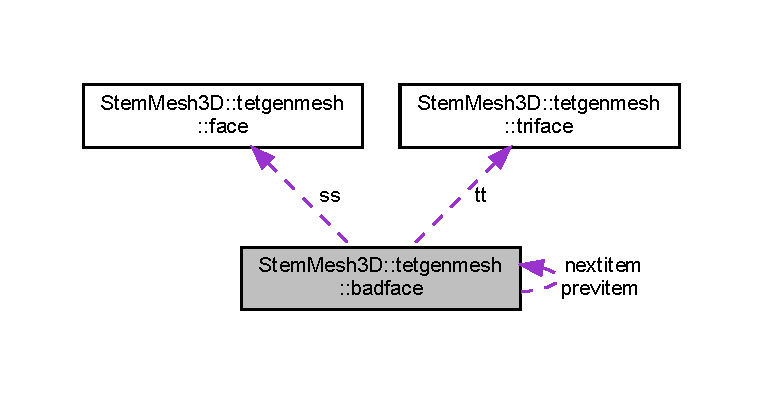
\includegraphics[width=350pt]{structStemMesh3D_1_1tetgenmesh_1_1badface__coll__graph}
\end{center}
\end{figure}
\doxysubsection*{Public Attributes}
\begin{DoxyCompactItemize}
\item 
\mbox{\Hypertarget{structStemMesh3D_1_1tetgenmesh_1_1badface_af014fdf9e448cbc8b9b5719b80a4a2be}\label{structStemMesh3D_1_1tetgenmesh_1_1badface_af014fdf9e448cbc8b9b5719b80a4a2be}} 
\mbox{\hyperlink{classStemMesh3D_1_1tetgenmesh_1_1triface}{triface}} {\bfseries tt}
\item 
\mbox{\Hypertarget{structStemMesh3D_1_1tetgenmesh_1_1badface_a83229333bab03814d19b09cbbee41793}\label{structStemMesh3D_1_1tetgenmesh_1_1badface_a83229333bab03814d19b09cbbee41793}} 
\mbox{\hyperlink{classStemMesh3D_1_1tetgenmesh_1_1face}{face}} {\bfseries ss}
\item 
\mbox{\Hypertarget{structStemMesh3D_1_1tetgenmesh_1_1badface_a709162edba7233cc9143dbd55af78895}\label{structStemMesh3D_1_1tetgenmesh_1_1badface_a709162edba7233cc9143dbd55af78895}} 
R\+E\+AL {\bfseries key}
\item 
\mbox{\Hypertarget{structStemMesh3D_1_1tetgenmesh_1_1badface_a0cd47500c3c0b3f337ce068c7a88d816}\label{structStemMesh3D_1_1tetgenmesh_1_1badface_a0cd47500c3c0b3f337ce068c7a88d816}} 
R\+E\+AL {\bfseries cent} \mbox{[}3\mbox{]}
\item 
\mbox{\Hypertarget{structStemMesh3D_1_1tetgenmesh_1_1badface_a25d78ab92fef52b647632598b9b71de7}\label{structStemMesh3D_1_1tetgenmesh_1_1badface_a25d78ab92fef52b647632598b9b71de7}} 
point {\bfseries forg}
\item 
\mbox{\Hypertarget{structStemMesh3D_1_1tetgenmesh_1_1badface_a12df5993ef6186c38566cfa12b809e7c}\label{structStemMesh3D_1_1tetgenmesh_1_1badface_a12df5993ef6186c38566cfa12b809e7c}} 
point {\bfseries fdest}
\item 
\mbox{\Hypertarget{structStemMesh3D_1_1tetgenmesh_1_1badface_aafc2b0921961b5fa93d57d3c707d5e43}\label{structStemMesh3D_1_1tetgenmesh_1_1badface_aafc2b0921961b5fa93d57d3c707d5e43}} 
point {\bfseries fapex}
\item 
\mbox{\Hypertarget{structStemMesh3D_1_1tetgenmesh_1_1badface_ae7051c51f1dd38db6aa77fbe5c8cc18c}\label{structStemMesh3D_1_1tetgenmesh_1_1badface_ae7051c51f1dd38db6aa77fbe5c8cc18c}} 
point {\bfseries foppo}
\item 
\mbox{\Hypertarget{structStemMesh3D_1_1tetgenmesh_1_1badface_aad785b95ee9a4d9dd3de87ad0712300c}\label{structStemMesh3D_1_1tetgenmesh_1_1badface_aad785b95ee9a4d9dd3de87ad0712300c}} 
point {\bfseries noppo}
\item 
\mbox{\Hypertarget{structStemMesh3D_1_1tetgenmesh_1_1badface_afa529346c673a03cf7719eeb012744c2}\label{structStemMesh3D_1_1tetgenmesh_1_1badface_afa529346c673a03cf7719eeb012744c2}} 
struct \mbox{\hyperlink{structStemMesh3D_1_1tetgenmesh_1_1badface}{badface}} $\ast$ {\bfseries previtem}
\item 
\mbox{\Hypertarget{structStemMesh3D_1_1tetgenmesh_1_1badface_a19265157bf24f08e058426b0fa700b86}\label{structStemMesh3D_1_1tetgenmesh_1_1badface_a19265157bf24f08e058426b0fa700b86}} 
struct \mbox{\hyperlink{structStemMesh3D_1_1tetgenmesh_1_1badface}{badface}} $\ast$ {\bfseries nextitem}
\end{DoxyCompactItemize}


The documentation for this struct was generated from the following file\+:\begin{DoxyCompactItemize}
\item 
src/\+Mesh/\+Stem\+Mesh/tetgen.\+h\end{DoxyCompactItemize}

\hypertarget{structHArDCore3D_1_1detail_1_1basis__evaluation__traits}{}\section{H\+Ar\+D\+Core3D\+:\+:detail\+:\+:basis\+\_\+evaluation\+\_\+traits$<$ Basis\+Type, Basis\+Function $>$ Struct Template Reference}
\label{structHArDCore3D_1_1detail_1_1basis__evaluation__traits}\index{H\+Ar\+D\+Core3\+D\+::detail\+::basis\+\_\+evaluation\+\_\+traits$<$ Basis\+Type, Basis\+Function $>$@{H\+Ar\+D\+Core3\+D\+::detail\+::basis\+\_\+evaluation\+\_\+traits$<$ Basis\+Type, Basis\+Function $>$}}


Basis evaluation traits. Only specializations are meaningful.  




{\ttfamily \#include $<$basis.\+hpp$>$}



\subsection{Detailed Description}
\subsubsection*{template$<$typename Basis\+Type, Basis\+FunctionE Basis\+Function$>$\newline
struct H\+Ar\+D\+Core3\+D\+::detail\+::basis\+\_\+evaluation\+\_\+traits$<$ Basis\+Type, Basis\+Function $>$}

Basis evaluation traits. Only specializations are meaningful. 

The documentation for this struct was generated from the following file\+:\begin{DoxyCompactItemize}
\item 
src/\+Common/basis.\+hpp\end{DoxyCompactItemize}

\hypertarget{structHArDCore3D_1_1detail_1_1basis__evaluation__traits_3_01BasisType_00_01Curl_01_4}{}\doxysection{H\+Ar\+D\+Core3D\+::detail\+::basis\+\_\+evaluation\+\_\+traits$<$ Basis\+Type, Curl $>$ Struct Template Reference}
\label{structHArDCore3D_1_1detail_1_1basis__evaluation__traits_3_01BasisType_00_01Curl_01_4}\index{HArDCore3D::detail::basis\_evaluation\_traits$<$ BasisType, Curl $>$@{HArDCore3D::detail::basis\_evaluation\_traits$<$ BasisType, Curl $>$}}
\doxysubsection*{Public Types}
\begin{DoxyCompactItemize}
\item 
typedef Basis\+Type\+::\+Curl\+Value {\bfseries Return\+Value}
\end{DoxyCompactItemize}
\doxysubsection*{Static Public Member Functions}
\begin{DoxyCompactItemize}
\item 
static Return\+Value {\bfseries evaluate} (const Basis\+Type \&basis, size\+\_\+t i, const Vector\+Rd \&x)
\item 
static Return\+Value {\bfseries evaluate} (const Basis\+Type \&basis, size\+\_\+t i, size\+\_\+t iqn, const boost\+::multi\+\_\+array$<$ Return\+Value, 2 $>$ \&ancestor\+\_\+curl\+\_\+quad)
\end{DoxyCompactItemize}


The documentation for this struct was generated from the following file\+:\begin{DoxyCompactItemize}
\item 
src/\+Common/basis.\+hpp\end{DoxyCompactItemize}

\hypertarget{structHArDCore3D_1_1detail_1_1basis__evaluation__traits_3_01BasisType_00_01Divergence_01_4}{}\section{H\+Ar\+D\+Core3D\+:\+:detail\+:\+:basis\+\_\+evaluation\+\_\+traits$<$ Basis\+Type, Divergence $>$ Struct Template Reference}
\label{structHArDCore3D_1_1detail_1_1basis__evaluation__traits_3_01BasisType_00_01Divergence_01_4}\index{H\+Ar\+D\+Core3\+D\+::detail\+::basis\+\_\+evaluation\+\_\+traits$<$ Basis\+Type, Divergence $>$@{H\+Ar\+D\+Core3\+D\+::detail\+::basis\+\_\+evaluation\+\_\+traits$<$ Basis\+Type, Divergence $>$}}
\subsection*{Public Types}
\begin{DoxyCompactItemize}
\item 
\mbox{\Hypertarget{structHArDCore3D_1_1detail_1_1basis__evaluation__traits_3_01BasisType_00_01Divergence_01_4_a1d8393298a710a4a0233017b265119e5}\label{structHArDCore3D_1_1detail_1_1basis__evaluation__traits_3_01BasisType_00_01Divergence_01_4_a1d8393298a710a4a0233017b265119e5}} 
typedef Basis\+Type\+::\+Divergence\+Value {\bfseries Return\+Value}
\end{DoxyCompactItemize}
\subsection*{Static Public Member Functions}
\begin{DoxyCompactItemize}
\item 
\mbox{\Hypertarget{structHArDCore3D_1_1detail_1_1basis__evaluation__traits_3_01BasisType_00_01Divergence_01_4_afd247472c237f7f2ef7f7cea9f887cd0}\label{structHArDCore3D_1_1detail_1_1basis__evaluation__traits_3_01BasisType_00_01Divergence_01_4_afd247472c237f7f2ef7f7cea9f887cd0}} 
static Return\+Value {\bfseries evaluate} (const Basis\+Type \&basis, size\+\_\+t i, const Vector\+Rd \&x)
\end{DoxyCompactItemize}


The documentation for this struct was generated from the following file\+:\begin{DoxyCompactItemize}
\item 
src/\+Common/basis.\+hpp\end{DoxyCompactItemize}

\hypertarget{structHArDCore3D_1_1detail_1_1basis__evaluation__traits_3_01BasisType_00_01Function_01_4}{}\section{H\+Ar\+D\+Core3D\+:\+:detail\+:\+:basis\+\_\+evaluation\+\_\+traits$<$ Basis\+Type, Function $>$ Struct Template Reference}
\label{structHArDCore3D_1_1detail_1_1basis__evaluation__traits_3_01BasisType_00_01Function_01_4}\index{H\+Ar\+D\+Core3\+D\+::detail\+::basis\+\_\+evaluation\+\_\+traits$<$ Basis\+Type, Function $>$@{H\+Ar\+D\+Core3\+D\+::detail\+::basis\+\_\+evaluation\+\_\+traits$<$ Basis\+Type, Function $>$}}
\subsection*{Public Types}
\begin{DoxyCompactItemize}
\item 
\mbox{\Hypertarget{structHArDCore3D_1_1detail_1_1basis__evaluation__traits_3_01BasisType_00_01Function_01_4_adb3235548ad3a366c5f950e8bbf86083}\label{structHArDCore3D_1_1detail_1_1basis__evaluation__traits_3_01BasisType_00_01Function_01_4_adb3235548ad3a366c5f950e8bbf86083}} 
typedef Basis\+Type\+::\+Function\+Value {\bfseries Return\+Value}
\end{DoxyCompactItemize}
\subsection*{Static Public Member Functions}
\begin{DoxyCompactItemize}
\item 
\mbox{\Hypertarget{structHArDCore3D_1_1detail_1_1basis__evaluation__traits_3_01BasisType_00_01Function_01_4_af68cac75a57525a28bebf726e03d4037}\label{structHArDCore3D_1_1detail_1_1basis__evaluation__traits_3_01BasisType_00_01Function_01_4_af68cac75a57525a28bebf726e03d4037}} 
static Return\+Value {\bfseries evaluate} (const Basis\+Type \&basis, size\+\_\+t i, const Vector\+Rd \&x)
\end{DoxyCompactItemize}


The documentation for this struct was generated from the following file\+:\begin{DoxyCompactItemize}
\item 
src/\+Common/basis.\+hpp\end{DoxyCompactItemize}

\hypertarget{structHArDCore3D_1_1detail_1_1basis__evaluation__traits_3_01BasisType_00_01Gradient_01_4}{}\section{H\+Ar\+D\+Core3D\+:\+:detail\+:\+:basis\+\_\+evaluation\+\_\+traits$<$ Basis\+Type, Gradient $>$ Struct Template Reference}
\label{structHArDCore3D_1_1detail_1_1basis__evaluation__traits_3_01BasisType_00_01Gradient_01_4}\index{H\+Ar\+D\+Core3\+D\+::detail\+::basis\+\_\+evaluation\+\_\+traits$<$ Basis\+Type, Gradient $>$@{H\+Ar\+D\+Core3\+D\+::detail\+::basis\+\_\+evaluation\+\_\+traits$<$ Basis\+Type, Gradient $>$}}
\subsection*{Public Types}
\begin{DoxyCompactItemize}
\item 
\mbox{\Hypertarget{structHArDCore3D_1_1detail_1_1basis__evaluation__traits_3_01BasisType_00_01Gradient_01_4_aebcec3c8eba77d1982728a44c6eb4f2e}\label{structHArDCore3D_1_1detail_1_1basis__evaluation__traits_3_01BasisType_00_01Gradient_01_4_aebcec3c8eba77d1982728a44c6eb4f2e}} 
typedef Basis\+Type\+::\+Gradient\+Value {\bfseries Return\+Value}
\end{DoxyCompactItemize}
\subsection*{Static Public Member Functions}
\begin{DoxyCompactItemize}
\item 
\mbox{\Hypertarget{structHArDCore3D_1_1detail_1_1basis__evaluation__traits_3_01BasisType_00_01Gradient_01_4_a1b36aa15e1d24a03d14e53c7f6c1fe1e}\label{structHArDCore3D_1_1detail_1_1basis__evaluation__traits_3_01BasisType_00_01Gradient_01_4_a1b36aa15e1d24a03d14e53c7f6c1fe1e}} 
static Return\+Value {\bfseries evaluate} (const Basis\+Type \&basis, size\+\_\+t i, const Vector\+Rd \&x)
\end{DoxyCompactItemize}


The documentation for this struct was generated from the following file\+:\begin{DoxyCompactItemize}
\item 
src/\+Common/basis.\+hpp\end{DoxyCompactItemize}

\hypertarget{classBoundaryConditions}{}\section{Boundary\+Conditions Class Reference}
\label{classBoundaryConditions}\index{Boundary\+Conditions@{Boundary\+Conditions}}


The \hyperlink{classBoundaryConditions}{Boundary\+Conditions} class provides definition of boundary conditions.  




{\ttfamily \#include $<$Boundary\+Conditions.\+hpp$>$}

\subsection*{Public Member Functions}
\begin{DoxyCompactItemize}
\item 
\hyperlink{classBoundaryConditions_a5f9b50ca35f0fcee51e84e015223396c}{Boundary\+Conditions} (const std\+::string bc\+\_\+id, \hyperlink{classHArDCore3D_1_1Mesh}{Mesh} \&mesh)
\begin{DoxyCompactList}\small\item\em Initialise data. \end{DoxyCompactList}\item 
const std\+::string \hyperlink{classBoundaryConditions_a2d4ed623f0f8b4585cbe75454777e14c}{type} (const \hyperlink{classHArDCore3D_1_1Face}{Face} \&face) const
\begin{DoxyCompactList}\small\item\em Test the boundary condition of an face. \end{DoxyCompactList}\item 
\mbox{\Hypertarget{classBoundaryConditions_af9e9493f0ba9be92b7299838bc08f0bf}\label{classBoundaryConditions_af9e9493f0ba9be92b7299838bc08f0bf}} 
const size\+\_\+t \hyperlink{classBoundaryConditions_af9e9493f0ba9be92b7299838bc08f0bf}{n\+\_\+dir\+\_\+faces} () const
\begin{DoxyCompactList}\small\item\em Returns the number of Dirichlet faces. \end{DoxyCompactList}\item 
\mbox{\Hypertarget{classBoundaryConditions_ac3609733d5e7e43e9240d0a8b05d17ba}\label{classBoundaryConditions_ac3609733d5e7e43e9240d0a8b05d17ba}} 
const std\+::string \hyperlink{classBoundaryConditions_ac3609733d5e7e43e9240d0a8b05d17ba}{name} () const
\begin{DoxyCompactList}\small\item\em Returns the complete name of the boundary condition. \end{DoxyCompactList}\item 
\mbox{\Hypertarget{classBoundaryConditions_a1898911b1e8e0b2832e2ce406b238d99}\label{classBoundaryConditions_a1898911b1e8e0b2832e2ce406b238d99}} 
void \hyperlink{classBoundaryConditions_a1898911b1e8e0b2832e2ce406b238d99}{reorder\+\_\+faces} ()
\begin{DoxyCompactList}\small\item\em Re-\/order faces of the mesh to put the Dirichlet faces at the end. \end{DoxyCompactList}\end{DoxyCompactItemize}


\subsection{Detailed Description}
The \hyperlink{classBoundaryConditions}{Boundary\+Conditions} class provides definition of boundary conditions. 

\subsection{Constructor \& Destructor Documentation}
\mbox{\Hypertarget{classBoundaryConditions_a5f9b50ca35f0fcee51e84e015223396c}\label{classBoundaryConditions_a5f9b50ca35f0fcee51e84e015223396c}} 
\index{Boundary\+Conditions@{Boundary\+Conditions}!Boundary\+Conditions@{Boundary\+Conditions}}
\index{Boundary\+Conditions@{Boundary\+Conditions}!Boundary\+Conditions@{Boundary\+Conditions}}
\subsubsection{\texorpdfstring{Boundary\+Conditions()}{BoundaryConditions()}}
{\footnotesize\ttfamily Boundary\+Conditions\+::\+Boundary\+Conditions (\begin{DoxyParamCaption}\item[{const std\+::string}]{bc\+\_\+id,  }\item[{\hyperlink{classHArDCore3D_1_1Mesh}{Mesh} \&}]{mesh }\end{DoxyParamCaption})}



Initialise data. 


\begin{DoxyParams}{Parameters}
{\em bc\+\_\+id} & The identifier for the boundary condition (D, N or Mx) \\
\hline
{\em mesh} & reference to the mesh \\
\hline
\end{DoxyParams}


\subsection{Member Function Documentation}
\mbox{\Hypertarget{classBoundaryConditions_a2d4ed623f0f8b4585cbe75454777e14c}\label{classBoundaryConditions_a2d4ed623f0f8b4585cbe75454777e14c}} 
\index{Boundary\+Conditions@{Boundary\+Conditions}!type@{type}}
\index{type@{type}!Boundary\+Conditions@{Boundary\+Conditions}}
\subsubsection{\texorpdfstring{type()}{type()}}
{\footnotesize\ttfamily const std\+::string Boundary\+Conditions\+::type (\begin{DoxyParamCaption}\item[{const \hyperlink{classHArDCore3D_1_1Face}{Face} \&}]{face }\end{DoxyParamCaption}) const}



Test the boundary condition of an face. 

\begin{DoxyReturn}{Returns}
\char`\"{}dir\char`\"{} or \char`\"{}neu\char`\"{} depending if the face is a Dirichlet or Neumann boundary condition, as determined by m\+\_\+bc\+\_\+id below. For an internal face, returns \char`\"{}int\char`\"{}. m\+\_\+bc\+\_\+id = \char`\"{}\+D\char`\"{}\+: all faces are Dirichlet m\+\_\+bc\+\_\+id = \char`\"{}\+N\char`\"{}\+: all faces are Neumann m\+\_\+bc\+\_\+id = \char`\"{}\+Mx\char`\"{} (x=0,1,...)\+: various types of mixed boundary conditions, some faces will be Dirichlet and some will be Neumman. 
\end{DoxyReturn}

\begin{DoxyParams}{Parameters}
{\em face} & Face on which to check the boundary condition \\
\hline
\end{DoxyParams}


The documentation for this class was generated from the following files\+:\begin{DoxyCompactItemize}
\item 
Schemes/\+Test\+Case/Boundary\+Conditions.\+hpp\item 
Schemes/\+Test\+Case/Boundary\+Conditions.\+cpp\end{DoxyCompactItemize}

\hypertarget{classHArDCore3D_1_1Cell}{}\doxysection{H\+Ar\+D\+Core3D\+::Cell Class Reference}
\label{classHArDCore3D_1_1Cell}\index{HArDCore3D::Cell@{HArDCore3D::Cell}}


The \mbox{\hyperlink{classHArDCore3D_1_1Cell}{Cell}} class provides description of a cell.  




{\ttfamily \#include $<$cell.\+hpp$>$}

\doxysubsection*{Public Member Functions}
\begin{DoxyCompactItemize}
\item 
\mbox{\hyperlink{group__Mesh_ga512c4d7f649bc03e64292394af0eeef2}{Cell}} (size\+\_\+t iC, \mbox{\hyperlink{classHArDCore3D_1_1Mesh}{Mesh}} $\ast$mesh, std\+::vector$<$ \mbox{\hyperlink{classHArDCore3D_1_1Face}{Face}} $\ast$ $>$ faces, std\+::vector$<$ \mbox{\hyperlink{classHArDCore3D_1_1Edge}{Edge}} $\ast$ $>$ edges, std\+::vector$<$ \mbox{\hyperlink{classHArDCore3D_1_1Vertex}{Vertex}} $\ast$ $>$ vertices, std\+::vector$<$ Vector3d $>$ face\+\_\+normals, bool boundary, double \mbox{\hyperlink{group__Mesh_ga75b939b8edadf100a35b9c7298fb5c8b}{measure}}, double \mbox{\hyperlink{group__Mesh_ga02b7103a8ceae610aa213334a6a1277d}{diam}}, Vector3d \mbox{\hyperlink{group__Mesh_ga3eb9c83b9578d3d93e94a698c37a980e}{center\+\_\+mass}})
\item 
size\+\_\+t \mbox{\hyperlink{group__Mesh_ga76cf6e2785020ff1cc8ec51bf4d232c5}{global\+\_\+index}} () const
\begin{DoxyCompactList}\small\item\em cell index \end{DoxyCompactList}\item 
size\+\_\+t \mbox{\hyperlink{group__Mesh_ga805584b31ee6aa7f6725075d8d16a744}{n\+\_\+faces}} () const
\begin{DoxyCompactList}\small\item\em returns number of faces of the cell \end{DoxyCompactList}\item 
size\+\_\+t \mbox{\hyperlink{group__Mesh_gad38d3b73d9e4aadcad92824c6a68d11b}{n\+\_\+edges}} () const
\begin{DoxyCompactList}\small\item\em returns number of edges of the cell \end{DoxyCompactList}\item 
size\+\_\+t \mbox{\hyperlink{group__Mesh_ga48af1867fb42455b120b608083e1aebc}{n\+\_\+vertices}} () const
\begin{DoxyCompactList}\small\item\em returns number of vertices of the cell \end{DoxyCompactList}\item 
std\+::vector$<$ \mbox{\hyperlink{classHArDCore3D_1_1Face}{Face}} $\ast$ $>$ \mbox{\hyperlink{group__Mesh_ga8c6361b9b63c0dbecb8189b43091207d}{get\+\_\+faces}} () const
\begin{DoxyCompactList}\small\item\em returns the list of faces of the cell \end{DoxyCompactList}\item 
std\+::vector$<$ \mbox{\hyperlink{classHArDCore3D_1_1Edge}{Edge}} $\ast$ $>$ \mbox{\hyperlink{group__Mesh_gabac3633d6b17df44320054664d9581b1}{get\+\_\+edges}} () const
\begin{DoxyCompactList}\small\item\em returns the list of edges of the cell \end{DoxyCompactList}\item 
std\+::vector$<$ \mbox{\hyperlink{classHArDCore3D_1_1Vertex}{Vertex}} $\ast$ $>$ \mbox{\hyperlink{group__Mesh_ga19a14fe5dd32fbf9d9557aaece6a0499}{get\+\_\+vertices}} () const
\begin{DoxyCompactList}\small\item\em returns the list of vertices of the cell \end{DoxyCompactList}\item 
std\+::vector$<$ \mbox{\hyperlink{classHArDCore3D_1_1Cell}{Cell}} $\ast$ $>$ \mbox{\hyperlink{group__Mesh_ga4d29dc1248424166380aa33d9ea7de3d}{get\+\_\+neighbours}} () const
\begin{DoxyCompactList}\small\item\em returns the list of neighbours of the cell \end{DoxyCompactList}\item 
\mbox{\hyperlink{classHArDCore3D_1_1Face}{Face}} $\ast$ \mbox{\hyperlink{group__Mesh_gae994179c36e882c6a9a6e80e9477bbb5}{face}} (size\+\_\+t iL) const
\begin{DoxyCompactList}\small\item\em returns the i\+L-\/th face of the cell \end{DoxyCompactList}\item 
\mbox{\hyperlink{classHArDCore3D_1_1Edge}{Edge}} $\ast$ \mbox{\hyperlink{group__Mesh_ga85defed1382a8af8227e89f00434603e}{edge}} (size\+\_\+t iL) const
\begin{DoxyCompactList}\small\item\em returns the i\+L-\/th edge of the cell \end{DoxyCompactList}\item 
\mbox{\hyperlink{classHArDCore3D_1_1Vertex}{Vertex}} $\ast$ \mbox{\hyperlink{group__Mesh_ga2e6bcdeac17fd028ef3892e7866c7b88}{vertex}} (size\+\_\+t iL) const
\begin{DoxyCompactList}\small\item\em returns the i\+L-\/th edge of the cell \end{DoxyCompactList}\item 
\mbox{\hyperlink{classHArDCore3D_1_1Cell}{Cell}} $\ast$ \mbox{\hyperlink{group__Mesh_gadddfffa330938bd8ab624349722a0e4e}{neighbour}} (size\+\_\+t iL) const
\begin{DoxyCompactList}\small\item\em returns the i\+L-\/th neighbour of the cell \end{DoxyCompactList}\item 
size\+\_\+t \mbox{\hyperlink{group__Mesh_ga35a0034e60d51c09e0f88e59b20a6b7a}{index\+\_\+face}} (const \mbox{\hyperlink{classHArDCore3D_1_1Face}{Face}} $\ast$F) const
\begin{DoxyCompactList}\small\item\em reciprocal of face(i)\+: returns the local index of face F in the cell ~\newline
 \end{DoxyCompactList}\item 
size\+\_\+t \mbox{\hyperlink{group__Mesh_ga64aa8d1d212339dc8e3222d36dc4c99f}{index\+\_\+edge}} (const \mbox{\hyperlink{classHArDCore3D_1_1Edge}{Edge}} $\ast$E) const
\begin{DoxyCompactList}\small\item\em reciprocal of edge(i)\+: returns the local index of edge E in the cell \end{DoxyCompactList}\item 
size\+\_\+t \mbox{\hyperlink{group__Mesh_ga97bc25d7764d00e93d3d2260636debed}{index\+\_\+vertex}} (const \mbox{\hyperlink{classHArDCore3D_1_1Vertex}{Vertex}} $\ast$V) const
\begin{DoxyCompactList}\small\item\em reciprocal of vertex(i)\+: returns the local index of vertex V in the cell \end{DoxyCompactList}\item 
bool \mbox{\hyperlink{group__Mesh_gab401dd009e7f13008b03cc2080d93449}{is\+\_\+boundary}} () const
\begin{DoxyCompactList}\small\item\em returns true if cell touches the boundary \end{DoxyCompactList}\item 
double \mbox{\hyperlink{group__Mesh_ga75b939b8edadf100a35b9c7298fb5c8b}{measure}} () const
\begin{DoxyCompactList}\small\item\em returns area of cell \end{DoxyCompactList}\item 
double \mbox{\hyperlink{group__Mesh_ga02b7103a8ceae610aa213334a6a1277d}{diam}} () const
\begin{DoxyCompactList}\small\item\em returns diameter of cell \end{DoxyCompactList}\item 
Vector3d \mbox{\hyperlink{group__Mesh_ga648c17f293071f01180c4014adb5a25b}{face\+\_\+normal}} (size\+\_\+t i) const
\begin{DoxyCompactList}\small\item\em returns the outer normal to the i-\/th face \end{DoxyCompactList}\item 
Vector3d \mbox{\hyperlink{group__Mesh_ga3eb9c83b9578d3d93e94a698c37a980e}{center\+\_\+mass}} () const
\begin{DoxyCompactList}\small\item\em returns the center of mass of the cell \end{DoxyCompactList}\item 
int \mbox{\hyperlink{group__Mesh_ga2bc91336489e3e8b98d9304972b65ba6}{face\+\_\+orientation}} (size\+\_\+t i) const
\begin{DoxyCompactList}\small\item\em returns the relative orientation of the i-\/th face with respect to the cell (that is, +1 if the normal to the face is the outer normal to the cell, -\/1 otherwise). \end{DoxyCompactList}\item 
bool \mbox{\hyperlink{group__Mesh_ga57e3ed95a38ecc546ead65e3c9d42820}{add\+\_\+face}} (\mbox{\hyperlink{classHArDCore3D_1_1Face}{Face}} $\ast$\mbox{\hyperlink{group__Mesh_gae994179c36e882c6a9a6e80e9477bbb5}{face}})
\begin{DoxyCompactList}\small\item\em add a face to the cell \end{DoxyCompactList}\item 
bool \mbox{\hyperlink{group__Mesh_gaa18b4bdf2f9217febcc96fc4415de1ce}{add\+\_\+edge}} (\mbox{\hyperlink{classHArDCore3D_1_1Edge}{Edge}} $\ast$\mbox{\hyperlink{group__Mesh_ga85defed1382a8af8227e89f00434603e}{edge}})
\begin{DoxyCompactList}\small\item\em add an edge to the cell \end{DoxyCompactList}\item 
bool \mbox{\hyperlink{group__Mesh_gaa4bebb4d2f23daaed37e1e1e2d464d01}{add\+\_\+vertex}} (\mbox{\hyperlink{classHArDCore3D_1_1Vertex}{Vertex}} $\ast$\mbox{\hyperlink{group__Mesh_ga2e6bcdeac17fd028ef3892e7866c7b88}{vertex}})
\begin{DoxyCompactList}\small\item\em add a vertex to the cell \end{DoxyCompactList}\item 
bool \mbox{\hyperlink{group__Mesh_ga6e29b140b5f4a286ed694f2851fe76e1}{add\+\_\+neighbour}} (\mbox{\hyperlink{classHArDCore3D_1_1Cell}{Cell}} $\ast$neigh)
\begin{DoxyCompactList}\small\item\em add a cell to the neighbour \end{DoxyCompactList}\item 
bool \mbox{\hyperlink{group__Mesh_ga6062f4f6764a978c5c3a645e1cb6a1bf}{add\+\_\+normal}} (Vector3d normal)
\begin{DoxyCompactList}\small\item\em add an outer normal to the cell \end{DoxyCompactList}\item 
void \mbox{\hyperlink{group__Mesh_gac4332b689450ab38b5c77ae9f5ff0809}{set\+\_\+boundary}} (bool val)
\begin{DoxyCompactList}\small\item\em Set the \+\_\+boundary value of the cell to val. \end{DoxyCompactList}\item 
void \mbox{\hyperlink{group__Mesh_ga65ac02c8ef4407d5c0693ae97d24c45a}{set\+\_\+global\+\_\+index}} (size\+\_\+t idx)
\begin{DoxyCompactList}\small\item\em Set the global index of the cell to idx. Used to re-\/index the cells, should essentially only be used inside \mbox{\hyperlink{group__Mesh_gaf77873bbc892a7a5b37bf4773c55aefc}{Mesh\+::renum}}. \end{DoxyCompactList}\end{DoxyCompactItemize}


\doxysubsection{Detailed Description}
The \mbox{\hyperlink{classHArDCore3D_1_1Cell}{Cell}} class provides description of a cell. 

The documentation for this class was generated from the following files\+:\begin{DoxyCompactItemize}
\item 
src/\+Mesh/cell.\+hpp\item 
src/\+Mesh/cell.\+cpp\end{DoxyCompactItemize}

\hypertarget{classHArDCore3D_1_1CurlBasis}{}\doxysection{H\+Ar\+D\+Core3D\+::Curl\+Basis$<$ Basis\+Type $>$ Class Template Reference}
\label{classHArDCore3D_1_1CurlBasis}\index{HArDCore3D::CurlBasis$<$ BasisType $>$@{HArDCore3D::CurlBasis$<$ BasisType $>$}}


Basis for the space of curls of polynomials.  




{\ttfamily \#include $<$basis.\+hpp$>$}

\doxysubsection*{Public Types}
\begin{DoxyCompactItemize}
\item 
typedef Vector\+Rd {\bfseries Function\+Value}
\item 
typedef Eigen\+::\+Matrix$<$ double, dimspace, dimspace $>$ {\bfseries Gradient\+Value}
\item 
typedef Eigen\+::\+Matrix$<$ double, dimspace, dimspace $>$ {\bfseries Curl\+Value}
\item 
typedef double {\bfseries Divergence\+Value}
\item 
typedef Basis\+Type\+::\+Geometric\+Support {\bfseries Geometric\+Support}
\end{DoxyCompactItemize}
\doxysubsection*{Public Member Functions}
\begin{DoxyCompactItemize}
\item 
\mbox{\hyperlink{group__Common_gaf0423afdb02f0b69b206709290b71325}{Curl\+Basis}} (const Basis\+Type \&basis)
\begin{DoxyCompactList}\small\item\em Constructor. \end{DoxyCompactList}\item 
size\+\_\+t \mbox{\hyperlink{group__Common_gaf49ecdf88a5895335f602276d81a805b}{dimension}} () const
\begin{DoxyCompactList}\small\item\em Compute the dimension of the basis. \end{DoxyCompactList}\item 
Function\+Value \mbox{\hyperlink{group__Common_ga5476b7c9f36899f48fdb549f25974b27}{function}} (size\+\_\+t i, const Vector\+Rd \&x) const
\begin{DoxyCompactList}\small\item\em Evaluate the i-\/th basis function at point x. \end{DoxyCompactList}\end{DoxyCompactItemize}
\doxysubsection*{Static Public Attributes}
\begin{DoxyCompactItemize}
\item 
static const Tensor\+RankE {\bfseries tensor\+Rank} = Vector
\item 
static const bool {\bfseries has\+Function} = true
\item 
static const bool {\bfseries has\+Gradient} = false
\item 
static const bool {\bfseries has\+Curl} = false
\item 
static const bool {\bfseries has\+Divergence} = false
\end{DoxyCompactItemize}


\doxysubsection{Detailed Description}
\subsubsection*{template$<$typename Basis\+Type$>$\newline
class H\+Ar\+D\+Core3\+D\+::\+Curl\+Basis$<$ Basis\+Type $>$}

Basis for the space of curls of polynomials. 

To construct a basis of R$^\wedge$k, assumes that the vector basis from which it is constructed is a basis for G$^\wedge$\{k+1,c\} (in 3D) or P$^\wedge$\{k+1\}/\+P$^\wedge$0 (in 2D) 

The documentation for this class was generated from the following file\+:\begin{DoxyCompactItemize}
\item 
src/\+Common/basis.\+hpp\end{DoxyCompactItemize}

\hypertarget{classHArDCore3D_1_1Edge}{}\section{H\+Ar\+D\+Core3D\+:\+:Edge Class Reference}
\label{classHArDCore3D_1_1Edge}\index{H\+Ar\+D\+Core3\+D\+::\+Edge@{H\+Ar\+D\+Core3\+D\+::\+Edge}}


The \hyperlink{classHArDCore3D_1_1Edge}{Edge} class provides description of an edge.  




{\ttfamily \#include $<$edge.\+hpp$>$}

\subsection*{Public Member Functions}
\begin{DoxyCompactItemize}
\item 
\hyperlink{classHArDCore3D_1_1Edge_a051ae1dd47537d89d8efbce3d4fd1760}{Edge} (size\+\_\+t iE, \hyperlink{classHArDCore3D_1_1Mesh}{Mesh} $\ast$mesh, std\+::vector$<$ \hyperlink{classHArDCore3D_1_1Vertex}{Vertex} $\ast$$>$ vertices, bool boundary, double \hyperlink{group__Mesh_ga38609361fcb95fa62e0bf2d5170144aa}{measure}, Vector3d \hyperlink{group__Mesh_gac7aee988662d982ab3fd81704af7842c}{center\+\_\+mass})
\item 
size\+\_\+t \hyperlink{group__Mesh_ga7460c422a7e7ed1a59bc930054551f68}{global\+\_\+index} () const
\begin{DoxyCompactList}\small\item\em returns the edge global index \end{DoxyCompactList}\item 
size\+\_\+t \hyperlink{group__Mesh_gabe29c7660cf7a1dddb06b876ebc76f80}{n\+\_\+cells} () const
\begin{DoxyCompactList}\small\item\em returns the number of cells neighbouring the edge \end{DoxyCompactList}\item 
size\+\_\+t \hyperlink{group__Mesh_gaab36400cd966cbeec90297f41c14ac55}{n\+\_\+faces} () const
\begin{DoxyCompactList}\small\item\em returns the number of faces neighbouring the edge \end{DoxyCompactList}\item 
\mbox{\Hypertarget{classHArDCore3D_1_1Edge_a72bedde2003c68d015c70326924b6d7f}\label{classHArDCore3D_1_1Edge_a72bedde2003c68d015c70326924b6d7f}} 
std\+::vector$<$ \hyperlink{classHArDCore3D_1_1Cell}{Cell} $\ast$ $>$ \hyperlink{classHArDCore3D_1_1Edge_a72bedde2003c68d015c70326924b6d7f}{get\+\_\+cells} () const
\begin{DoxyCompactList}\small\item\em list of cells that are neighbours of the edge \end{DoxyCompactList}\item 
\mbox{\Hypertarget{classHArDCore3D_1_1Edge_a67aee2c97080416a5bbff937275a6c67}\label{classHArDCore3D_1_1Edge_a67aee2c97080416a5bbff937275a6c67}} 
std\+::vector$<$ \hyperlink{classHArDCore3D_1_1Face}{Face} $\ast$ $>$ \hyperlink{classHArDCore3D_1_1Edge_a67aee2c97080416a5bbff937275a6c67}{get\+\_\+faces} () const
\begin{DoxyCompactList}\small\item\em list of faces of the edge \end{DoxyCompactList}\item 
\mbox{\Hypertarget{classHArDCore3D_1_1Edge_a5315c7fa0058509166d75175660ed542}\label{classHArDCore3D_1_1Edge_a5315c7fa0058509166d75175660ed542}} 
std\+::vector$<$ \hyperlink{classHArDCore3D_1_1Vertex}{Vertex} $\ast$ $>$ \hyperlink{classHArDCore3D_1_1Edge_a5315c7fa0058509166d75175660ed542}{get\+\_\+vertices} () const
\begin{DoxyCompactList}\small\item\em list of vertices of the edge \end{DoxyCompactList}\item 
\mbox{\Hypertarget{classHArDCore3D_1_1Edge_ad4be0bfb981ccf2c1e02e870772dbdc3}\label{classHArDCore3D_1_1Edge_ad4be0bfb981ccf2c1e02e870772dbdc3}} 
\hyperlink{classHArDCore3D_1_1Cell}{Cell} $\ast$ \hyperlink{classHArDCore3D_1_1Edge_ad4be0bfb981ccf2c1e02e870772dbdc3}{cell} (size\+\_\+t i) const
\begin{DoxyCompactList}\small\item\em returns pointer to the i-\/th cell neighbour of the edge \end{DoxyCompactList}\item 
\mbox{\Hypertarget{classHArDCore3D_1_1Edge_a84a3891c3abf7f441f2787943e0e0f66}\label{classHArDCore3D_1_1Edge_a84a3891c3abf7f441f2787943e0e0f66}} 
\hyperlink{classHArDCore3D_1_1Face}{Face} $\ast$ \hyperlink{classHArDCore3D_1_1Edge_a84a3891c3abf7f441f2787943e0e0f66}{face} (size\+\_\+t i) const
\begin{DoxyCompactList}\small\item\em returns pointer to the i-\/th face neighbour of the edge \end{DoxyCompactList}\item 
\mbox{\Hypertarget{classHArDCore3D_1_1Edge_ade257bc049ec1f43751fc647e07ec052}\label{classHArDCore3D_1_1Edge_ade257bc049ec1f43751fc647e07ec052}} 
\hyperlink{classHArDCore3D_1_1Vertex}{Vertex} $\ast$ \hyperlink{classHArDCore3D_1_1Edge_ade257bc049ec1f43751fc647e07ec052}{vertex} (size\+\_\+t i) const
\begin{DoxyCompactList}\small\item\em returns a pointer to the i-\/th vertex of the edge \end{DoxyCompactList}\item 
\mbox{\Hypertarget{classHArDCore3D_1_1Edge_a9801b008f6b5d356c257589945171ec2}\label{classHArDCore3D_1_1Edge_a9801b008f6b5d356c257589945171ec2}} 
size\+\_\+t \hyperlink{classHArDCore3D_1_1Edge_a9801b008f6b5d356c257589945171ec2}{index\+\_\+vertex} (\hyperlink{classHArDCore3D_1_1Vertex}{Vertex} $\ast$V) const
\begin{DoxyCompactList}\small\item\em reciprocal of vertex(i)\+: returns the local index of vertex V in the edge \end{DoxyCompactList}\item 
double \hyperlink{group__Mesh_ga38609361fcb95fa62e0bf2d5170144aa}{measure} () const
\begin{DoxyCompactList}\small\item\em length of the edge \end{DoxyCompactList}\item 
double \hyperlink{group__Mesh_ga93672b9685e10344c31cdae234017557}{diam} () const
\begin{DoxyCompactList}\small\item\em length of the edge \end{DoxyCompactList}\item 
Vector3d \hyperlink{group__Mesh_gac7aee988662d982ab3fd81704af7842c}{center\+\_\+mass} () const
\begin{DoxyCompactList}\small\item\em get the midpoint of the edge \end{DoxyCompactList}\item 
\mbox{\Hypertarget{classHArDCore3D_1_1Edge_a5af3b015940acca0b35e8960161ba592}\label{classHArDCore3D_1_1Edge_a5af3b015940acca0b35e8960161ba592}} 
Vector3d \hyperlink{classHArDCore3D_1_1Edge_a5af3b015940acca0b35e8960161ba592}{tangent} () const
\begin{DoxyCompactList}\small\item\em $<$ get the normalised tangent to the edge, oriented from the first vertex to the second vertex. \end{DoxyCompactList}\item 
bool \hyperlink{group__Mesh_ga2caaa7859e84eab62858ff8c24d261fe}{is\+\_\+boundary} () const
\begin{DoxyCompactList}\small\item\em getter to see if edge is boundary edge \end{DoxyCompactList}\item 
\mbox{\Hypertarget{classHArDCore3D_1_1Edge_a364bacf89dfa0be36abbbadbb2dd4f78}\label{classHArDCore3D_1_1Edge_a364bacf89dfa0be36abbbadbb2dd4f78}} 
void \hyperlink{classHArDCore3D_1_1Edge_a364bacf89dfa0be36abbbadbb2dd4f78}{add\+\_\+cell} (\hyperlink{classHArDCore3D_1_1Cell}{Cell} $\ast$\hyperlink{classHArDCore3D_1_1Edge_ad4be0bfb981ccf2c1e02e870772dbdc3}{cell})
\begin{DoxyCompactList}\small\item\em Add a new cell to the edge. \end{DoxyCompactList}\item 
\mbox{\Hypertarget{classHArDCore3D_1_1Edge_a7758bf6587d0153b7c9e63d088b61157}\label{classHArDCore3D_1_1Edge_a7758bf6587d0153b7c9e63d088b61157}} 
void \hyperlink{classHArDCore3D_1_1Edge_a7758bf6587d0153b7c9e63d088b61157}{add\+\_\+face} (\hyperlink{classHArDCore3D_1_1Face}{Face} $\ast$\hyperlink{classHArDCore3D_1_1Edge_a84a3891c3abf7f441f2787943e0e0f66}{face})
\begin{DoxyCompactList}\small\item\em Add a new face to the edge. \end{DoxyCompactList}\item 
\mbox{\Hypertarget{classHArDCore3D_1_1Edge_a8902091c785b5857648f5c9ba55f6eba}\label{classHArDCore3D_1_1Edge_a8902091c785b5857648f5c9ba55f6eba}} 
void \hyperlink{classHArDCore3D_1_1Edge_a8902091c785b5857648f5c9ba55f6eba}{add\+\_\+vertex} (\hyperlink{classHArDCore3D_1_1Vertex}{Vertex} $\ast$\hyperlink{classHArDCore3D_1_1Edge_ade257bc049ec1f43751fc647e07ec052}{vertex})
\begin{DoxyCompactList}\small\item\em Add a new vertex to the edge. \end{DoxyCompactList}\item 
\mbox{\Hypertarget{classHArDCore3D_1_1Edge_aed492c6f6fa58b06262ecfa0420121e3}\label{classHArDCore3D_1_1Edge_aed492c6f6fa58b06262ecfa0420121e3}} 
void \hyperlink{classHArDCore3D_1_1Edge_aed492c6f6fa58b06262ecfa0420121e3}{set\+\_\+boundary} (bool val)
\begin{DoxyCompactList}\small\item\em Set the \+\_\+boundary value of the face to val. \end{DoxyCompactList}\item 
\mbox{\Hypertarget{classHArDCore3D_1_1Edge_a150b8b31cd1b608d6ce8b020227a6db2}\label{classHArDCore3D_1_1Edge_a150b8b31cd1b608d6ce8b020227a6db2}} 
void \hyperlink{classHArDCore3D_1_1Edge_a150b8b31cd1b608d6ce8b020227a6db2}{set\+\_\+global\+\_\+index} (size\+\_\+t idx)
\begin{DoxyCompactList}\small\item\em Set the global index of the edge to idx. Used to re-\/index the edges, should essentially only be used inside \hyperlink{classHArDCore3D_1_1Mesh_af77873bbc892a7a5b37bf4773c55aefc}{Mesh\+::renum}. \end{DoxyCompactList}\end{DoxyCompactItemize}


\subsection{Detailed Description}
The \hyperlink{classHArDCore3D_1_1Edge}{Edge} class provides description of an edge. 

\subsection{Constructor \& Destructor Documentation}
\mbox{\Hypertarget{classHArDCore3D_1_1Edge_a051ae1dd47537d89d8efbce3d4fd1760}\label{classHArDCore3D_1_1Edge_a051ae1dd47537d89d8efbce3d4fd1760}} 
\index{H\+Ar\+D\+Core3\+D\+::\+Edge@{H\+Ar\+D\+Core3\+D\+::\+Edge}!Edge@{Edge}}
\index{Edge@{Edge}!H\+Ar\+D\+Core3\+D\+::\+Edge@{H\+Ar\+D\+Core3\+D\+::\+Edge}}
\subsubsection{\texorpdfstring{Edge()}{Edge()}}
{\footnotesize\ttfamily Edge\+::\+Edge (\begin{DoxyParamCaption}\item[{size\+\_\+t}]{iE,  }\item[{\hyperlink{classHArDCore3D_1_1Mesh}{Mesh} $\ast$}]{mesh,  }\item[{std\+::vector$<$ \hyperlink{classHArDCore3D_1_1Vertex}{Vertex} $\ast$$>$}]{vertices,  }\item[{bool}]{boundary,  }\item[{double}]{measure,  }\item[{Vector3d}]{center\+\_\+mass }\end{DoxyParamCaption})}

A class representing an edge of a 3D mesh. Contains a pointer to the mesh, as well as to the cells, faces and vertices connected to that edge Constructor. Edges are constructed after vertices, so these can be feed into the constructor.


\begin{DoxyParams}{Parameters}
{\em iE} & global edge number \\
\hline
{\em mesh} & pointer to the mesh \\
\hline
{\em vertices} & vertices of the edge \\
\hline
{\em measure} & length of the edge \\
\hline
{\em center\+\_\+mass} & midpoint of the edge \\
\hline
\end{DoxyParams}


The documentation for this class was generated from the following files\+:\begin{DoxyCompactItemize}
\item 
src/\+Mesh/edge.\+hpp\item 
src/\+Mesh/edge.\+cpp\end{DoxyCompactItemize}

\hypertarget{structStemMesh3D_1_1edge__struct}{}\doxysection{Stem\+Mesh3D\+::edge\+\_\+struct Struct Reference}
\label{structStemMesh3D_1_1edge__struct}\index{StemMesh3D::edge\_struct@{StemMesh3D::edge\_struct}}
\doxysubsection*{Public Member Functions}
\begin{DoxyCompactItemize}
\item 
\mbox{\Hypertarget{structStemMesh3D_1_1edge__struct_a72f6a67fcca5f9773b3c51629297451f}\label{structStemMesh3D_1_1edge__struct_a72f6a67fcca5f9773b3c51629297451f}} 
{\bfseries edge\+\_\+struct} (size\+\_\+t \+\_\+\+V0, size\+\_\+t \+\_\+\+V1, size\+\_\+t \+\_\+iF, size\+\_\+t \+\_\+ilF)
\end{DoxyCompactItemize}
\doxysubsection*{Public Attributes}
\begin{DoxyCompactItemize}
\item 
\mbox{\Hypertarget{structStemMesh3D_1_1edge__struct_ae8eeed6a7553815472116d2a7b7a6699}\label{structStemMesh3D_1_1edge__struct_ae8eeed6a7553815472116d2a7b7a6699}} 
size\+\_\+t {\bfseries V0}
\item 
\mbox{\Hypertarget{structStemMesh3D_1_1edge__struct_a753424fef6b438026e10d86ceb39b4f9}\label{structStemMesh3D_1_1edge__struct_a753424fef6b438026e10d86ceb39b4f9}} 
size\+\_\+t {\bfseries V1}
\item 
\mbox{\Hypertarget{structStemMesh3D_1_1edge__struct_a20680666adeadc5ab4632469084efe06}\label{structStemMesh3D_1_1edge__struct_a20680666adeadc5ab4632469084efe06}} 
size\+\_\+t {\bfseries iF}
\item 
\mbox{\Hypertarget{structStemMesh3D_1_1edge__struct_a51c6031bf4c5705d4d83787a15dd897c}\label{structStemMesh3D_1_1edge__struct_a51c6031bf4c5705d4d83787a15dd897c}} 
size\+\_\+t {\bfseries ilF}
\item 
\mbox{\Hypertarget{structStemMesh3D_1_1edge__struct_ad9e56beb0f51457b362cef4841185dde}\label{structStemMesh3D_1_1edge__struct_ad9e56beb0f51457b362cef4841185dde}} 
bool {\bfseries bval}
\end{DoxyCompactItemize}


The documentation for this struct was generated from the following file\+:\begin{DoxyCompactItemize}
\item 
src/\+Mesh/\+Stem\+Mesh/builder.\+hh\end{DoxyCompactItemize}

\hypertarget{classHArDCore3D_1_1ElementQuad}{}\section{H\+Ar\+D\+Core3D\+:\+:Element\+Quad Class Reference}
\label{classHArDCore3D_1_1ElementQuad}\index{H\+Ar\+D\+Core3\+D\+::\+Element\+Quad@{H\+Ar\+D\+Core3\+D\+::\+Element\+Quad}}


{\ttfamily \#include $<$elementquad.\+hpp$>$}

\subsection*{Public Member Functions}
\begin{DoxyCompactItemize}
\item 
\hyperlink{classHArDCore3D_1_1ElementQuad_a0d27ba99f9f3e6f2a3e5311e6be19eba}{Element\+Quad} (const \hyperlink{classHArDCore3D_1_1HybridCore}{Hybrid\+Core} \&hho, const size\+\_\+t iT, const size\+\_\+t doeT, const size\+\_\+t doeF)
\begin{DoxyCompactList}\small\item\em Class constructor\+: loads the quadrature rules and values of basis functions/gradients at these points. \end{DoxyCompactList}\item 
Quadrature\+Rule \hyperlink{group__HybridCore_ga9676c87f42764a058c9d7aecd2ce44cd}{get\+\_\+quadT} () const
\begin{DoxyCompactList}\small\item\em Returns quadrature rules in cell. \end{DoxyCompactList}\item 
std\+::vector$<$ Eigen\+::\+Array\+Xd $>$ \hyperlink{group__HybridCore_gaafce6cb00f061fe1159a9972b73d3bb9}{get\+\_\+phi\+T\+\_\+quadT} () const
\begin{DoxyCompactList}\small\item\em Returns values of cell basis functions at cell quadrature rules in cell. \end{DoxyCompactList}\item 
std\+::vector$<$ Eigen\+::\+Array\+X\+Xd $>$ \hyperlink{group__HybridCore_gab0450891cb0d96686256c31e87948374}{get\+\_\+dphi\+T\+\_\+quadT} () const
\begin{DoxyCompactList}\small\item\em Returns values of gradients of cell basis functions at cell quadrature rules in cell. \end{DoxyCompactList}\item 
Quadrature\+Rule \hyperlink{group__HybridCore_ga7eb693a2f8d58d04b0e653cb952e59f2}{get\+\_\+quadF} (size\+\_\+t ilF) const
\begin{DoxyCompactList}\small\item\em Returns quadrature rules on face with local number ilF. \end{DoxyCompactList}\item 
std\+::vector$<$ Eigen\+::\+Array\+Xd $>$ \hyperlink{group__HybridCore_gab6349fe3a8eb0d4070cd2bd82742bdcc}{get\+\_\+phi\+T\+\_\+quadF} (size\+\_\+t ilF) const
\begin{DoxyCompactList}\small\item\em Returns values of cell basis functions at cell quadrature rules on face with local number ilF. \end{DoxyCompactList}\item 
std\+::vector$<$ Eigen\+::\+Array\+Xd $>$ \hyperlink{group__HybridCore_gad9c2ba4cdbfda183ee00ab059d8885e5}{get\+\_\+phi\+F\+\_\+quadF} (size\+\_\+t ilF) const
\begin{DoxyCompactList}\small\item\em Returns values of faces basis functions at face quadrature rules on face with local number ilF. \end{DoxyCompactList}\item 
std\+::vector$<$ Eigen\+::\+Array\+X\+Xd $>$ \hyperlink{group__HybridCore_gabae2f4323f94acb5417ca82870790071}{get\+\_\+dphi\+T\+\_\+quadF} (size\+\_\+t ilF) const
\begin{DoxyCompactList}\small\item\em Returns values of gradients of cell basis functions at cell quadrature rules on face with local number ilF. \end{DoxyCompactList}\item 
std\+::vector$<$ Eigen\+::\+Array\+X\+Xd $>$ \hyperlink{classHArDCore3D_1_1ElementQuad_a0df097bcb15554c9f9ee752f04c14f95}{get\+\_\+vec\+\_\+phi\+T\+\_\+quadT} (size\+\_\+t degree) const
\begin{DoxyCompactList}\small\item\em Builds on the fly the values of cell basis functions at cell quadrature nodes. The vector basis is obtained by tensorization of the scalar one\+: (phi\+\_\+0,0,0), (phi\+\_\+1,0,0), ..., (phi\+\_\+N,0,0), (0,phi\+\_\+0,0), (0,phi\+\_\+1,0) ... (0,phi\+\_\+N,0), (0,0,phi\+\_\+0) ... (0,0,phi\+\_\+N). \end{DoxyCompactList}\item 
std\+::vector$<$ Eigen\+::\+Array\+X\+Xd $>$ \hyperlink{classHArDCore3D_1_1ElementQuad_a318c36aca48d3cdb6b501d3d0e1554cf}{get\+\_\+vec\+\_\+phi\+T\+\_\+quadF} (size\+\_\+t ilF, size\+\_\+t degree) const
\begin{DoxyCompactList}\small\item\em Builds on the fly the values of cell basis functions at face quadrature nodes. The vector basis is obtained by tensorization of the scalar one\+: (phi\+\_\+0,0,0), (phi\+\_\+1,0,0), ..., (phi\+\_\+N,0,0), (0,phi\+\_\+0,0), (0,phi\+\_\+1,0) ... (0,phi\+\_\+N,0), (0,0,phi\+\_\+0) ... (0,0,phi\+\_\+N). \end{DoxyCompactList}\item 
std\+::vector$<$ Eigen\+::\+Array\+X\+Xd $>$ \hyperlink{classHArDCore3D_1_1ElementQuad_a1a9a6bf14079608b3f706136568d3e7d}{get\+\_\+vec\+\_\+phi\+F\+\_\+quadF} (size\+\_\+t ilF, size\+\_\+t degree) const
\begin{DoxyCompactList}\small\item\em Builds on the fly the values of face basis functions at face quadrature nodes. The vector basis is obtained by tensorization of the scalar one\+: (phi\+\_\+0,0,0), (phi\+\_\+1,0,0), ..., (phi\+\_\+N,0,0), (0,phi\+\_\+0,0), (0,phi\+\_\+1,0) ... (0,phi\+\_\+N,0), (0,0,phi\+\_\+0) ... (0,0,phi\+\_\+N). \end{DoxyCompactList}\end{DoxyCompactItemize}


\subsection{Detailed Description}
The \hyperlink{classHArDCore3D_1_1ElementQuad}{Element\+Quad} class creates cell and face quadrature rules, and vectors of values of basis functions and gradients at these points 

\subsection{Constructor \& Destructor Documentation}
\mbox{\Hypertarget{classHArDCore3D_1_1ElementQuad_a0d27ba99f9f3e6f2a3e5311e6be19eba}\label{classHArDCore3D_1_1ElementQuad_a0d27ba99f9f3e6f2a3e5311e6be19eba}} 
\index{H\+Ar\+D\+Core3\+D\+::\+Element\+Quad@{H\+Ar\+D\+Core3\+D\+::\+Element\+Quad}!Element\+Quad@{Element\+Quad}}
\index{Element\+Quad@{Element\+Quad}!H\+Ar\+D\+Core3\+D\+::\+Element\+Quad@{H\+Ar\+D\+Core3\+D\+::\+Element\+Quad}}
\subsubsection{\texorpdfstring{Element\+Quad()}{ElementQuad()}}
{\footnotesize\ttfamily Element\+Quad\+::\+Element\+Quad (\begin{DoxyParamCaption}\item[{const \hyperlink{classHArDCore3D_1_1HybridCore}{Hybrid\+Core} \&}]{hho,  }\item[{const size\+\_\+t}]{iT,  }\item[{const size\+\_\+t}]{doeT,  }\item[{const size\+\_\+t}]{doeF }\end{DoxyParamCaption})}



Class constructor\+: loads the quadrature rules and values of basis functions/gradients at these points. 


\begin{DoxyParams}{Parameters}
{\em hho} & A reference to the hybridcore instance \\
\hline
{\em iT} & Number of cell \\
\hline
{\em doeT} & The degree of exactness for cell quadratures \\
\hline
{\em doeF} & The degree of exactness of face quadratures \\
\hline
\end{DoxyParams}


\subsection{Member Function Documentation}
\mbox{\Hypertarget{classHArDCore3D_1_1ElementQuad_a1a9a6bf14079608b3f706136568d3e7d}\label{classHArDCore3D_1_1ElementQuad_a1a9a6bf14079608b3f706136568d3e7d}} 
\index{H\+Ar\+D\+Core3\+D\+::\+Element\+Quad@{H\+Ar\+D\+Core3\+D\+::\+Element\+Quad}!get\+\_\+vec\+\_\+phi\+F\+\_\+quadF@{get\+\_\+vec\+\_\+phi\+F\+\_\+quadF}}
\index{get\+\_\+vec\+\_\+phi\+F\+\_\+quadF@{get\+\_\+vec\+\_\+phi\+F\+\_\+quadF}!H\+Ar\+D\+Core3\+D\+::\+Element\+Quad@{H\+Ar\+D\+Core3\+D\+::\+Element\+Quad}}
\subsubsection{\texorpdfstring{get\+\_\+vec\+\_\+phi\+F\+\_\+quad\+F()}{get\_vec\_phiF\_quadF()}}
{\footnotesize\ttfamily std\+::vector$<$ Eigen\+::\+Array\+X\+Xd $>$ Element\+Quad\+::get\+\_\+vec\+\_\+phi\+F\+\_\+quadF (\begin{DoxyParamCaption}\item[{size\+\_\+t}]{ilF,  }\item[{size\+\_\+t}]{degree }\end{DoxyParamCaption}) const}



Builds on the fly the values of face basis functions at face quadrature nodes. The vector basis is obtained by tensorization of the scalar one\+: (phi\+\_\+0,0,0), (phi\+\_\+1,0,0), ..., (phi\+\_\+N,0,0), (0,phi\+\_\+0,0), (0,phi\+\_\+1,0) ... (0,phi\+\_\+N,0), (0,0,phi\+\_\+0) ... (0,0,phi\+\_\+N). 

\begin{DoxyReturn}{Returns}
vec\+\_\+phi\+T\+\_\+quadT such that, for r=0,..,dim-\/1 and i=0,..,dim\+\_\+\+Pcell(degree)-\/1, vec\+\_\+phi\+T\+\_\+quadT\mbox{[}r$\ast$dim\+\_\+\+Pcell(degree)-\/1 + i\mbox{]} has, on its row r, the values of the i-\/th scalar basis function at the quadrature nodes, and 0 on its other rows. 
\end{DoxyReturn}

\begin{DoxyParams}{Parameters}
{\em degree} & local number of face required degree of basis function \\
\hline
\end{DoxyParams}
\mbox{\Hypertarget{classHArDCore3D_1_1ElementQuad_a318c36aca48d3cdb6b501d3d0e1554cf}\label{classHArDCore3D_1_1ElementQuad_a318c36aca48d3cdb6b501d3d0e1554cf}} 
\index{H\+Ar\+D\+Core3\+D\+::\+Element\+Quad@{H\+Ar\+D\+Core3\+D\+::\+Element\+Quad}!get\+\_\+vec\+\_\+phi\+T\+\_\+quadF@{get\+\_\+vec\+\_\+phi\+T\+\_\+quadF}}
\index{get\+\_\+vec\+\_\+phi\+T\+\_\+quadF@{get\+\_\+vec\+\_\+phi\+T\+\_\+quadF}!H\+Ar\+D\+Core3\+D\+::\+Element\+Quad@{H\+Ar\+D\+Core3\+D\+::\+Element\+Quad}}
\subsubsection{\texorpdfstring{get\+\_\+vec\+\_\+phi\+T\+\_\+quad\+F()}{get\_vec\_phiT\_quadF()}}
{\footnotesize\ttfamily std\+::vector$<$ Eigen\+::\+Array\+X\+Xd $>$ Element\+Quad\+::get\+\_\+vec\+\_\+phi\+T\+\_\+quadF (\begin{DoxyParamCaption}\item[{size\+\_\+t}]{ilF,  }\item[{size\+\_\+t}]{degree }\end{DoxyParamCaption}) const}



Builds on the fly the values of cell basis functions at face quadrature nodes. The vector basis is obtained by tensorization of the scalar one\+: (phi\+\_\+0,0,0), (phi\+\_\+1,0,0), ..., (phi\+\_\+N,0,0), (0,phi\+\_\+0,0), (0,phi\+\_\+1,0) ... (0,phi\+\_\+N,0), (0,0,phi\+\_\+0) ... (0,0,phi\+\_\+N). 

\begin{DoxyReturn}{Returns}
vec\+\_\+phi\+T\+\_\+quadT such that, for r=0,..,dim-\/1 and i=0,..,dim\+\_\+\+Pcell(degree)-\/1, vec\+\_\+phi\+T\+\_\+quadT\mbox{[}r$\ast$dim\+\_\+\+Pcell(degree)-\/1 + i\mbox{]} has, on its row r, the values of the i-\/th scalar basis function at the quadrature nodes, and 0 on its other rows. 
\end{DoxyReturn}

\begin{DoxyParams}{Parameters}
{\em degree} & local number of face maximum degree of basis functions required \\
\hline
\end{DoxyParams}
\mbox{\Hypertarget{classHArDCore3D_1_1ElementQuad_a0df097bcb15554c9f9ee752f04c14f95}\label{classHArDCore3D_1_1ElementQuad_a0df097bcb15554c9f9ee752f04c14f95}} 
\index{H\+Ar\+D\+Core3\+D\+::\+Element\+Quad@{H\+Ar\+D\+Core3\+D\+::\+Element\+Quad}!get\+\_\+vec\+\_\+phi\+T\+\_\+quadT@{get\+\_\+vec\+\_\+phi\+T\+\_\+quadT}}
\index{get\+\_\+vec\+\_\+phi\+T\+\_\+quadT@{get\+\_\+vec\+\_\+phi\+T\+\_\+quadT}!H\+Ar\+D\+Core3\+D\+::\+Element\+Quad@{H\+Ar\+D\+Core3\+D\+::\+Element\+Quad}}
\subsubsection{\texorpdfstring{get\+\_\+vec\+\_\+phi\+T\+\_\+quad\+T()}{get\_vec\_phiT\_quadT()}}
{\footnotesize\ttfamily std\+::vector$<$ Eigen\+::\+Array\+X\+Xd $>$ Element\+Quad\+::get\+\_\+vec\+\_\+phi\+T\+\_\+quadT (\begin{DoxyParamCaption}\item[{size\+\_\+t}]{degree }\end{DoxyParamCaption}) const}



Builds on the fly the values of cell basis functions at cell quadrature nodes. The vector basis is obtained by tensorization of the scalar one\+: (phi\+\_\+0,0,0), (phi\+\_\+1,0,0), ..., (phi\+\_\+N,0,0), (0,phi\+\_\+0,0), (0,phi\+\_\+1,0) ... (0,phi\+\_\+N,0), (0,0,phi\+\_\+0) ... (0,0,phi\+\_\+N). 

\begin{DoxyReturn}{Returns}
vec\+\_\+phi\+T\+\_\+quadT such that, for r=0,..,dim-\/1 and i=0,..,dim\+\_\+\+Pcell(degree)-\/1, vec\+\_\+phi\+T\+\_\+quadT\mbox{[}r$\ast$dim\+\_\+\+Pcell(degree)-\/1 + i\mbox{]} has, on its row r, the values of the i-\/th scalar basis function at the quadrature nodes, and 0 on its other rows. 
\end{DoxyReturn}

\begin{DoxyParams}{Parameters}
{\em degree} & maximal degree of basis functions that is required \\
\hline
\end{DoxyParams}


The documentation for this class was generated from the following files\+:\begin{DoxyCompactItemize}
\item 
src/\+Hybrid\+Core/elementquad.\+hpp\item 
src/\+Hybrid\+Core/elementquad.\+cpp\end{DoxyCompactItemize}

\hypertarget{structHArDCore3D_1_1evaluate__quad}{}\section{H\+Ar\+D\+Core3D\+:\+:evaluate\+\_\+quad$<$ Basis\+Function $>$ Struct Template Reference}
\label{structHArDCore3D_1_1evaluate__quad}\index{H\+Ar\+D\+Core3\+D\+::evaluate\+\_\+quad$<$ Basis\+Function $>$@{H\+Ar\+D\+Core3\+D\+::evaluate\+\_\+quad$<$ Basis\+Function $>$}}


{\ttfamily \#include $<$basis.\+hpp$>$}

\subsection*{Static Public Member Functions}
\begin{DoxyCompactItemize}
\item 
{\footnotesize template$<$typename Basis\+Type $>$ }\\static boost\+::multi\+\_\+array$<$ typename \hyperlink{structHArDCore3D_1_1detail_1_1basis__evaluation__traits}{detail\+::basis\+\_\+evaluation\+\_\+traits}$<$ Basis\+Type, Basis\+Function $>$\+::Return\+Value, 2 $>$ \hyperlink{structHArDCore3D_1_1evaluate__quad_a1abe06df2a8a25ad4de2f738930ec143}{compute} (const Basis\+Type \&basis, const Quadrature\+Rule \&quad)
\begin{DoxyCompactList}\small\item\em Generic basis evaluation. \end{DoxyCompactList}\item 
{\footnotesize template$<$typename Basis\+Type $>$ }\\static boost\+::multi\+\_\+array$<$ typename \hyperlink{structHArDCore3D_1_1detail_1_1basis__evaluation__traits}{detail\+::basis\+\_\+evaluation\+\_\+traits}$<$ \hyperlink{classHArDCore3D_1_1Family}{Family}$<$ Basis\+Type $>$, Basis\+Function $>$\+::Return\+Value, 2 $>$ \hyperlink{structHArDCore3D_1_1evaluate__quad_aa1df24802a0b4781d1c7e8203f772a52}{compute} (const \hyperlink{classHArDCore3D_1_1Family}{Family}$<$ Basis\+Type $>$ \&basis, const Quadrature\+Rule \&quad)
\end{DoxyCompactItemize}


\subsection{Detailed Description}
\subsubsection*{template$<$Basis\+FunctionE Basis\+Function$>$\newline
struct H\+Ar\+D\+Core3\+D\+::evaluate\+\_\+quad$<$ Basis\+Function $>$}

Evaluate a basis at quadrature nodes. \textquotesingle{}Basis\+Function\textquotesingle{} determines what kind of value we want to evaluate (the function value of the basis, their gradients, etc.). 

\subsection{Member Function Documentation}
\mbox{\Hypertarget{structHArDCore3D_1_1evaluate__quad_a1abe06df2a8a25ad4de2f738930ec143}\label{structHArDCore3D_1_1evaluate__quad_a1abe06df2a8a25ad4de2f738930ec143}} 
\index{H\+Ar\+D\+Core3\+D\+::evaluate\+\_\+quad@{H\+Ar\+D\+Core3\+D\+::evaluate\+\_\+quad}!compute@{compute}}
\index{compute@{compute}!H\+Ar\+D\+Core3\+D\+::evaluate\+\_\+quad@{H\+Ar\+D\+Core3\+D\+::evaluate\+\_\+quad}}
\subsubsection{\texorpdfstring{compute()}{compute()}\hspace{0.1cm}{\footnotesize\ttfamily [1/2]}}
{\footnotesize\ttfamily template$<$Basis\+FunctionE Basis\+Function$>$ \\
template$<$typename Basis\+Type $>$ \\
static boost\+::multi\+\_\+array$<$typename \hyperlink{structHArDCore3D_1_1detail_1_1basis__evaluation__traits}{detail\+::basis\+\_\+evaluation\+\_\+traits}$<$Basis\+Type, Basis\+Function$>$\+::Return\+Value, 2$>$ \hyperlink{structHArDCore3D_1_1evaluate__quad}{H\+Ar\+D\+Core3\+D\+::evaluate\+\_\+quad}$<$ Basis\+Function $>$\+::compute (\begin{DoxyParamCaption}\item[{const Basis\+Type \&}]{basis,  }\item[{const Quadrature\+Rule \&}]{quad }\end{DoxyParamCaption})\hspace{0.3cm}{\ttfamily [inline]}, {\ttfamily [static]}}



Generic basis evaluation. 


\begin{DoxyParams}{Parameters}
{\em basis} & The basis \\
\hline
{\em quad} & The quadrature rule \\
\hline
\end{DoxyParams}
\mbox{\Hypertarget{structHArDCore3D_1_1evaluate__quad_aa1df24802a0b4781d1c7e8203f772a52}\label{structHArDCore3D_1_1evaluate__quad_aa1df24802a0b4781d1c7e8203f772a52}} 
\index{H\+Ar\+D\+Core3\+D\+::evaluate\+\_\+quad@{H\+Ar\+D\+Core3\+D\+::evaluate\+\_\+quad}!compute@{compute}}
\index{compute@{compute}!H\+Ar\+D\+Core3\+D\+::evaluate\+\_\+quad@{H\+Ar\+D\+Core3\+D\+::evaluate\+\_\+quad}}
\subsubsection{\texorpdfstring{compute()}{compute()}\hspace{0.1cm}{\footnotesize\ttfamily [2/2]}}
{\footnotesize\ttfamily template$<$Basis\+FunctionE Basis\+Function$>$ \\
template$<$typename Basis\+Type $>$ \\
static boost\+::multi\+\_\+array$<$typename \hyperlink{structHArDCore3D_1_1detail_1_1basis__evaluation__traits}{detail\+::basis\+\_\+evaluation\+\_\+traits}$<$\hyperlink{classHArDCore3D_1_1Family}{Family}$<$Basis\+Type$>$, Basis\+Function$>$\+::Return\+Value, 2$>$ \hyperlink{structHArDCore3D_1_1evaluate__quad}{H\+Ar\+D\+Core3\+D\+::evaluate\+\_\+quad}$<$ Basis\+Function $>$\+::compute (\begin{DoxyParamCaption}\item[{const \hyperlink{classHArDCore3D_1_1Family}{Family}$<$ Basis\+Type $>$ \&}]{basis,  }\item[{const Quadrature\+Rule \&}]{quad }\end{DoxyParamCaption})\hspace{0.3cm}{\ttfamily [inline]}, {\ttfamily [static]}}

Evaluate a family at quadrature nodes. Same as \textquotesingle{}\hyperlink{structHArDCore3D_1_1evaluate__quad}{evaluate\+\_\+quad}\textquotesingle{} but applied to a family given by an ancestor basis and a matrix (see class \textquotesingle{}\hyperlink{classHArDCore3D_1_1Family}{Family}\textquotesingle{}) 
\begin{DoxyParams}{Parameters}
{\em basis} & The family \\
\hline
{\em quad} & The quadrature rule \\
\hline
\end{DoxyParams}


The documentation for this struct was generated from the following file\+:\begin{DoxyCompactItemize}
\item 
src/\+Common/basis.\+hpp\end{DoxyCompactItemize}

\hypertarget{classStemMesh3D_1_1ExtFileInput}{}\section{Stem\+Mesh3D\+:\+:Ext\+File\+Input Class Reference}
\label{classStemMesh3D_1_1ExtFileInput}\index{Stem\+Mesh3\+D\+::\+Ext\+File\+Input@{Stem\+Mesh3\+D\+::\+Ext\+File\+Input}}


Reads mesh files from a variety of file formats and loads them into a mesh object.  




{\ttfamily \#include $<$mesh3\+D\+\_\+greader.\+hh$>$}

\subsection*{Public Member Functions}
\begin{DoxyCompactItemize}
\item 
void \hyperlink{classStemMesh3D_1_1ExtFileInput_af553f539c3337a0e8bcdc6140c5b4911}{T\+E\+T\+G\+E\+N\+\_\+format} (\hyperlink{classStemMesh3D_1_1mesh__3Dv}{mesh\+\_\+3\+Dv} \&mesh, std\+::string fname=\char`\"{}mesh\char`\"{}, size\+\_\+t offset=C\+\_\+offset)
\begin{DoxyCompactList}\small\item\em Read a 3D mesh in the T\+E\+T\+G\+EN format. \end{DoxyCompactList}\item 
void \hyperlink{classStemMesh3D_1_1ExtFileInput_ae89dd2d6f641d108ec15b435ba62d62e}{R\+E\+G\+N\+\_\+\+F\+A\+C\+E\+\_\+format} (\hyperlink{classStemMesh3D_1_1mesh__3Dv}{mesh\+\_\+3\+Dv} \&mesh, std\+::string fname=\char`\"{}mesh\char`\"{}, size\+\_\+t offset=C\+\_\+offset)
\begin{DoxyCompactList}\small\item\em Read a 3D mesh in the R\+E\+GN F\+A\+CE format. \end{DoxyCompactList}\item 
void \hyperlink{classStemMesh3D_1_1ExtFileInput_a1a601ea2d05672f64588ac167cfe4a28}{M\+S\+H\+\_\+format} (\hyperlink{classStemMesh3D_1_1mesh__3Dv}{mesh\+\_\+3\+Dv} \&mesh, std\+::string fname=\char`\"{}mesh\char`\"{}, size\+\_\+t offset=F\+\_\+offset)
\begin{DoxyCompactList}\small\item\em Read a 3D mesh in the M\+SH format. \end{DoxyCompactList}\item 
void \hyperlink{classStemMesh3D_1_1ExtFileInput_a54db829a85fd1d52d02e47714949ea16}{multi\+\_\+layer\+\_\+format} (\hyperlink{classStemMesh3D_1_1mesh__3Dv}{mesh\+\_\+3\+Dv} \&mesh, std\+::string fname=\char`\"{}mesh\char`\"{}, size\+\_\+t n\+\_\+layer=1, size\+\_\+t offset=C\+\_\+offset)
\begin{DoxyCompactList}\small\item\em Read a general 2D mesh and build a layered 3D mesh from it. \end{DoxyCompactList}\end{DoxyCompactItemize}


\subsection{Detailed Description}
Reads mesh files from a variety of file formats and loads them into a mesh object. 

\subsection{Member Function Documentation}
\mbox{\Hypertarget{classStemMesh3D_1_1ExtFileInput_a1a601ea2d05672f64588ac167cfe4a28}\label{classStemMesh3D_1_1ExtFileInput_a1a601ea2d05672f64588ac167cfe4a28}} 
\index{Stem\+Mesh3\+D\+::\+Ext\+File\+Input@{Stem\+Mesh3\+D\+::\+Ext\+File\+Input}!M\+S\+H\+\_\+format@{M\+S\+H\+\_\+format}}
\index{M\+S\+H\+\_\+format@{M\+S\+H\+\_\+format}!Stem\+Mesh3\+D\+::\+Ext\+File\+Input@{Stem\+Mesh3\+D\+::\+Ext\+File\+Input}}
\subsubsection{\texorpdfstring{M\+S\+H\+\_\+format()}{MSH\_format()}}
{\footnotesize\ttfamily void Stem\+Mesh3\+D\+::\+Ext\+File\+Input\+::\+M\+S\+H\+\_\+format (\begin{DoxyParamCaption}\item[{\hyperlink{classStemMesh3D_1_1mesh__3Dv}{mesh\+\_\+3\+Dv} \&}]{mesh,  }\item[{std\+::string}]{fname = {\ttfamily \char`\"{}mesh\char`\"{}},  }\item[{size\+\_\+t}]{offset = {\ttfamily F\+\_\+offset} }\end{DoxyParamCaption})}



Read a 3D mesh in the M\+SH format. 


\begin{DoxyParams}{Parameters}
{\em mesh} & The mesh object to load the mesh in to \\
\hline
{\em fname} & The filename of the mesh file \\
\hline
{\em offset} & The indexing offset used in the file (1 = 1-\/based indexing etc.) \\
\hline
\end{DoxyParams}
\mbox{\Hypertarget{classStemMesh3D_1_1ExtFileInput_a54db829a85fd1d52d02e47714949ea16}\label{classStemMesh3D_1_1ExtFileInput_a54db829a85fd1d52d02e47714949ea16}} 
\index{Stem\+Mesh3\+D\+::\+Ext\+File\+Input@{Stem\+Mesh3\+D\+::\+Ext\+File\+Input}!multi\+\_\+layer\+\_\+format@{multi\+\_\+layer\+\_\+format}}
\index{multi\+\_\+layer\+\_\+format@{multi\+\_\+layer\+\_\+format}!Stem\+Mesh3\+D\+::\+Ext\+File\+Input@{Stem\+Mesh3\+D\+::\+Ext\+File\+Input}}
\subsubsection{\texorpdfstring{multi\+\_\+layer\+\_\+format()}{multi\_layer\_format()}}
{\footnotesize\ttfamily void Stem\+Mesh3\+D\+::\+Ext\+File\+Input\+::multi\+\_\+layer\+\_\+format (\begin{DoxyParamCaption}\item[{\hyperlink{classStemMesh3D_1_1mesh__3Dv}{mesh\+\_\+3\+Dv} \&}]{mesh,  }\item[{std\+::string}]{fname = {\ttfamily \char`\"{}mesh\char`\"{}},  }\item[{size\+\_\+t}]{n\+\_\+layer = {\ttfamily 1},  }\item[{size\+\_\+t}]{offset = {\ttfamily C\+\_\+offset} }\end{DoxyParamCaption})}



Read a general 2D mesh and build a layered 3D mesh from it. 


\begin{DoxyParams}{Parameters}
{\em mesh} & The mesh object to load the mesh in to \\
\hline
{\em fname} & The filename of the mesh file \\
\hline
{\em n\+\_\+layer} & The number of layers to put in the mesh \\
\hline
{\em offset} & The indexing offset used in the file (1 = 1-\/based indexing etc.) \\
\hline
\end{DoxyParams}
\mbox{\Hypertarget{classStemMesh3D_1_1ExtFileInput_ae89dd2d6f641d108ec15b435ba62d62e}\label{classStemMesh3D_1_1ExtFileInput_ae89dd2d6f641d108ec15b435ba62d62e}} 
\index{Stem\+Mesh3\+D\+::\+Ext\+File\+Input@{Stem\+Mesh3\+D\+::\+Ext\+File\+Input}!R\+E\+G\+N\+\_\+\+F\+A\+C\+E\+\_\+format@{R\+E\+G\+N\+\_\+\+F\+A\+C\+E\+\_\+format}}
\index{R\+E\+G\+N\+\_\+\+F\+A\+C\+E\+\_\+format@{R\+E\+G\+N\+\_\+\+F\+A\+C\+E\+\_\+format}!Stem\+Mesh3\+D\+::\+Ext\+File\+Input@{Stem\+Mesh3\+D\+::\+Ext\+File\+Input}}
\subsubsection{\texorpdfstring{R\+E\+G\+N\+\_\+\+F\+A\+C\+E\+\_\+format()}{REGN\_FACE\_format()}}
{\footnotesize\ttfamily void Stem\+Mesh3\+D\+::\+Ext\+File\+Input\+::\+R\+E\+G\+N\+\_\+\+F\+A\+C\+E\+\_\+format (\begin{DoxyParamCaption}\item[{\hyperlink{classStemMesh3D_1_1mesh__3Dv}{mesh\+\_\+3\+Dv} \&}]{mesh,  }\item[{std\+::string}]{fname = {\ttfamily \char`\"{}mesh\char`\"{}},  }\item[{size\+\_\+t}]{offset = {\ttfamily C\+\_\+offset} }\end{DoxyParamCaption})}



Read a 3D mesh in the R\+E\+GN F\+A\+CE format. 


\begin{DoxyParams}{Parameters}
{\em mesh} & The mesh object to load the mesh in to \\
\hline
{\em fname} & The filename of the mesh file \\
\hline
{\em offset} & The indexing offset used in the file (1 = 1-\/based indexing etc.) \\
\hline
\end{DoxyParams}
\mbox{\Hypertarget{classStemMesh3D_1_1ExtFileInput_af553f539c3337a0e8bcdc6140c5b4911}\label{classStemMesh3D_1_1ExtFileInput_af553f539c3337a0e8bcdc6140c5b4911}} 
\index{Stem\+Mesh3\+D\+::\+Ext\+File\+Input@{Stem\+Mesh3\+D\+::\+Ext\+File\+Input}!T\+E\+T\+G\+E\+N\+\_\+format@{T\+E\+T\+G\+E\+N\+\_\+format}}
\index{T\+E\+T\+G\+E\+N\+\_\+format@{T\+E\+T\+G\+E\+N\+\_\+format}!Stem\+Mesh3\+D\+::\+Ext\+File\+Input@{Stem\+Mesh3\+D\+::\+Ext\+File\+Input}}
\subsubsection{\texorpdfstring{T\+E\+T\+G\+E\+N\+\_\+format()}{TETGEN\_format()}}
{\footnotesize\ttfamily void Stem\+Mesh3\+D\+::\+Ext\+File\+Input\+::\+T\+E\+T\+G\+E\+N\+\_\+format (\begin{DoxyParamCaption}\item[{\hyperlink{classStemMesh3D_1_1mesh__3Dv}{mesh\+\_\+3\+Dv} \&}]{mesh,  }\item[{std\+::string}]{fname = {\ttfamily \char`\"{}mesh\char`\"{}},  }\item[{size\+\_\+t}]{offset = {\ttfamily C\+\_\+offset} }\end{DoxyParamCaption})}



Read a 3D mesh in the T\+E\+T\+G\+EN format. 


\begin{DoxyParams}{Parameters}
{\em mesh} & The mesh object to load the mesh in to \\
\hline
{\em fname} & The filename of the mesh file \\
\hline
{\em offset} & The indexing offset used in the file (1 = 1-\/based indexing etc.) \\
\hline
\end{DoxyParams}


The documentation for this class was generated from the following file\+:\begin{DoxyCompactItemize}
\item 
src/\+Mesh/\+Stem\+Mesh/mesh3\+D\+\_\+greader.\+hh\end{DoxyCompactItemize}

\hypertarget{classHArDCore3D_1_1Face}{}\doxysection{H\+Ar\+D\+Core3D\+::Face Class Reference}
\label{classHArDCore3D_1_1Face}\index{HArDCore3D::Face@{HArDCore3D::Face}}


The \mbox{\hyperlink{classHArDCore3D_1_1Face}{Face}} class provides description of an edge.  




{\ttfamily \#include $<$face.\+hpp$>$}

\doxysubsection*{Public Member Functions}
\begin{DoxyCompactItemize}
\item 
\mbox{\hyperlink{group__Mesh_gaf581dda7ff692d3732c5e0944ac46ab0}{Face}} (size\+\_\+t iF, \mbox{\hyperlink{classHArDCore3D_1_1Mesh}{Mesh}} $\ast$mesh, std\+::vector$<$ \mbox{\hyperlink{classHArDCore3D_1_1Edge}{Edge}} $\ast$ $>$ edges, std\+::vector$<$ \mbox{\hyperlink{classHArDCore3D_1_1Vertex}{Vertex}} $\ast$ $>$ vertices, bool boundary, double \mbox{\hyperlink{group__Mesh_gad8284631ae078f8f5a15147b7b1014a1}{measure}}, double \mbox{\hyperlink{group__Mesh_ga3303318a9f1465bf279617959644b01a}{diam}}, Vector3d \mbox{\hyperlink{group__Mesh_gac5d883f4f09a9af506924638939bb35a}{center\+\_\+mass}}, Vector3d \mbox{\hyperlink{group__Mesh_gaf2b13fd21cb283d14878c2ea25727e1f}{normal}})
\item 
size\+\_\+t \mbox{\hyperlink{group__Mesh_ga5cf9000fd94ae2e7ec79245607644f1b}{global\+\_\+index}} () const
\begin{DoxyCompactList}\small\item\em returns the face global index \end{DoxyCompactList}\item 
size\+\_\+t \mbox{\hyperlink{group__Mesh_ga5407c36b8a6d8d8bf64e8fd559cebbe9}{n\+\_\+cells}} () const
\begin{DoxyCompactList}\small\item\em returns the number of cells neighbouring the face \end{DoxyCompactList}\item 
size\+\_\+t \mbox{\hyperlink{group__Mesh_gaab27135cdfd18bc7dae7f01715a4edc6}{n\+\_\+edges}} () const
\begin{DoxyCompactList}\small\item\em returns the number of edges neighbouring the face \end{DoxyCompactList}\item 
size\+\_\+t \mbox{\hyperlink{group__Mesh_ga50edc49af3d9f7433e238e9d18f7f11c}{n\+\_\+vertices}} () const
\begin{DoxyCompactList}\small\item\em returns the number of vertices neighbouring the face \end{DoxyCompactList}\item 
std\+::vector$<$ \mbox{\hyperlink{classHArDCore3D_1_1Cell}{Cell}} $\ast$ $>$ \mbox{\hyperlink{group__Mesh_gaa209c78a79161da020d96bdd752d8e87}{get\+\_\+cells}} () const
\begin{DoxyCompactList}\small\item\em list of cells that are neighbours of the face \end{DoxyCompactList}\item 
std\+::vector$<$ \mbox{\hyperlink{classHArDCore3D_1_1Edge}{Edge}} $\ast$ $>$ \mbox{\hyperlink{group__Mesh_gabb3add94aa880748646382717345c1ec}{get\+\_\+edges}} () const
\begin{DoxyCompactList}\small\item\em list of edges of the face \end{DoxyCompactList}\item 
std\+::vector$<$ \mbox{\hyperlink{classHArDCore3D_1_1Vertex}{Vertex}} $\ast$ $>$ \mbox{\hyperlink{group__Mesh_ga4be6533a35079c67abfedc8dd65d01f1}{get\+\_\+vertices}} () const
\begin{DoxyCompactList}\small\item\em list of vertices of the face \end{DoxyCompactList}\item 
\mbox{\hyperlink{classHArDCore3D_1_1Cell}{Cell}} $\ast$ \mbox{\hyperlink{group__Mesh_gab463b4972c43d6f62f034cf8c0ed70c2}{cell}} (size\+\_\+t i) const
\begin{DoxyCompactList}\small\item\em returns pointer to the i-\/th cell neighbour of the face \end{DoxyCompactList}\item 
\mbox{\hyperlink{classHArDCore3D_1_1Edge}{Edge}} $\ast$ \mbox{\hyperlink{group__Mesh_ga93dd83df13314df283be122c36b93c29}{edge}} (size\+\_\+t i) const
\begin{DoxyCompactList}\small\item\em returns a pointer to the i-\/th edge of the face \end{DoxyCompactList}\item 
\mbox{\hyperlink{classHArDCore3D_1_1Vertex}{Vertex}} $\ast$ \mbox{\hyperlink{group__Mesh_ga63c8254509d075b402e1ce7393efd70c}{vertex}} (size\+\_\+t i) const
\begin{DoxyCompactList}\small\item\em returns a pointer to the i-\/th vertex of the face \end{DoxyCompactList}\item 
size\+\_\+t \mbox{\hyperlink{group__Mesh_ga9fafed8814ff199fbbe5995ff4de3067}{index\+\_\+edge}} (const \mbox{\hyperlink{classHArDCore3D_1_1Edge}{Edge}} $\ast$E) const
\begin{DoxyCompactList}\small\item\em reciprocal of edge(i)\+: returns the local index of edge E in the face \end{DoxyCompactList}\item 
size\+\_\+t \mbox{\hyperlink{group__Mesh_gabecb40cdeec22fee088921e66aa86800}{index\+\_\+vertex}} (const \mbox{\hyperlink{classHArDCore3D_1_1Vertex}{Vertex}} $\ast$V) const
\begin{DoxyCompactList}\small\item\em reciprocal of vertex(i)\+: returns the local index of vertex V in the face \end{DoxyCompactList}\item 
Vector3d \mbox{\hyperlink{group__Mesh_ga8cf04b618dccb40a61ee8144edd9610e}{edge\+\_\+normal}} (size\+\_\+t i) const
\begin{DoxyCompactList}\small\item\em returns the normal to the i-\/th edge in the plane spanned by the face. This is not necessarily the outer normal to the face. To obtain this outer normal, multiply by edge\+\_\+orientation(i). \end{DoxyCompactList}\item 
int \mbox{\hyperlink{group__Mesh_gaa02d3eab7ba590dec07134da1f85dbeb}{edge\+\_\+orientation}} (size\+\_\+t i) const
\begin{DoxyCompactList}\small\item\em returns the orientation of the i-\/th edge. It is the number such that edge\+\_\+orientation $\ast$ edge\+\_\+normal is the outer normal to the face. \end{DoxyCompactList}\item 
double \mbox{\hyperlink{group__Mesh_gad8284631ae078f8f5a15147b7b1014a1}{measure}} () const
\begin{DoxyCompactList}\small\item\em measure of the face \end{DoxyCompactList}\item 
double \mbox{\hyperlink{group__Mesh_ga3303318a9f1465bf279617959644b01a}{diam}} () const
\begin{DoxyCompactList}\small\item\em returns diameter of face \end{DoxyCompactList}\item 
Vector3d \mbox{\hyperlink{group__Mesh_gac5d883f4f09a9af506924638939bb35a}{center\+\_\+mass}} () const
\begin{DoxyCompactList}\small\item\em get the center of mass of the face \end{DoxyCompactList}\item 
Vector3d \mbox{\hyperlink{group__Mesh_gaf2b13fd21cb283d14878c2ea25727e1f}{normal}} () const
\begin{DoxyCompactList}\small\item\em get the normal to the face \end{DoxyCompactList}\item 
bool \mbox{\hyperlink{group__Mesh_ga8f69df15c3c76b4f80f51231ede670f5}{is\+\_\+boundary}} () const
\begin{DoxyCompactList}\small\item\em getter to see if the face is a boundary face \end{DoxyCompactList}\item 
void \mbox{\hyperlink{group__Mesh_ga0c4cc1b593b288e6c70747b6481824f8}{add\+\_\+cell}} (\mbox{\hyperlink{classHArDCore3D_1_1Cell}{Cell}} $\ast$\mbox{\hyperlink{group__Mesh_gab463b4972c43d6f62f034cf8c0ed70c2}{cell}})
\begin{DoxyCompactList}\small\item\em Add a cell to the face. \end{DoxyCompactList}\item 
void \mbox{\hyperlink{group__Mesh_ga0f3dd04f1ab142689e76165d8824c428}{add\+\_\+edge}} (\mbox{\hyperlink{classHArDCore3D_1_1Edge}{Edge}} $\ast$\mbox{\hyperlink{group__Mesh_ga93dd83df13314df283be122c36b93c29}{edge}})
\begin{DoxyCompactList}\small\item\em Add a edge to the face. \end{DoxyCompactList}\item 
void \mbox{\hyperlink{group__Mesh_ga7b9f09bcce8fc3beb56634e0793af83f}{add\+\_\+vertex}} (\mbox{\hyperlink{classHArDCore3D_1_1Vertex}{Vertex}} $\ast$\mbox{\hyperlink{group__Mesh_ga63c8254509d075b402e1ce7393efd70c}{vertex}})
\begin{DoxyCompactList}\small\item\em Add a vertex to the face. \end{DoxyCompactList}\item 
void \mbox{\hyperlink{group__Mesh_gafdd39678036c46f979da9909419c3428}{set\+\_\+boundary}} (bool val)
\begin{DoxyCompactList}\small\item\em Set the \+\_\+boundary value of the face to val. \end{DoxyCompactList}\item 
void \mbox{\hyperlink{group__Mesh_ga66289e0a31138cfce6ac948f09423548}{set\+\_\+global\+\_\+index}} (size\+\_\+t idx)
\begin{DoxyCompactList}\small\item\em Set the global index of the face to idx. Used to re-\/index the faces, should essentially only be used inside \mbox{\hyperlink{group__Mesh_gaf77873bbc892a7a5b37bf4773c55aefc}{Mesh\+::renum}}. \end{DoxyCompactList}\end{DoxyCompactItemize}


\doxysubsection{Detailed Description}
The \mbox{\hyperlink{classHArDCore3D_1_1Face}{Face}} class provides description of an edge. 

The documentation for this class was generated from the following files\+:\begin{DoxyCompactItemize}
\item 
src/\+Mesh/face.\+hpp\item 
src/\+Mesh/face.\+cpp\end{DoxyCompactItemize}

\hypertarget{classStemMesh3D_1_1tetgenmesh_1_1face}{}\section{Stem\+Mesh3D\+:\+:tetgenmesh\+:\+:face Class Reference}
\label{classStemMesh3D_1_1tetgenmesh_1_1face}\index{Stem\+Mesh3\+D\+::tetgenmesh\+::face@{Stem\+Mesh3\+D\+::tetgenmesh\+::face}}
\subsection*{Public Member Functions}
\begin{DoxyCompactItemize}
\item 
\mbox{\Hypertarget{classStemMesh3D_1_1tetgenmesh_1_1face_a1c9f12be9677eed2dfb2e4a7e0377a43}\label{classStemMesh3D_1_1tetgenmesh_1_1face_a1c9f12be9677eed2dfb2e4a7e0377a43}} 
\hyperlink{classStemMesh3D_1_1tetgenmesh_1_1face}{face} \& {\bfseries operator=} (const \hyperlink{classStemMesh3D_1_1tetgenmesh_1_1face}{face} \&s)
\item 
\mbox{\Hypertarget{classStemMesh3D_1_1tetgenmesh_1_1face_a5870f2ca141bdf00100d459bce96f904}\label{classStemMesh3D_1_1tetgenmesh_1_1face_a5870f2ca141bdf00100d459bce96f904}} 
bool {\bfseries operator==} (\hyperlink{classStemMesh3D_1_1tetgenmesh_1_1face}{face} \&s)
\item 
\mbox{\Hypertarget{classStemMesh3D_1_1tetgenmesh_1_1face_aa93c4956efb5323ce6e5ec1ef8e6d108}\label{classStemMesh3D_1_1tetgenmesh_1_1face_aa93c4956efb5323ce6e5ec1ef8e6d108}} 
bool {\bfseries operator!=} (\hyperlink{classStemMesh3D_1_1tetgenmesh_1_1face}{face} \&s)
\end{DoxyCompactItemize}
\subsection*{Public Attributes}
\begin{DoxyCompactItemize}
\item 
\mbox{\Hypertarget{classStemMesh3D_1_1tetgenmesh_1_1face_af81d93597724b3319c0b5e51e1d89665}\label{classStemMesh3D_1_1tetgenmesh_1_1face_af81d93597724b3319c0b5e51e1d89665}} 
shellface $\ast$ {\bfseries sh}
\item 
\mbox{\Hypertarget{classStemMesh3D_1_1tetgenmesh_1_1face_aff1fa90784a7d7998549cf4854971dad}\label{classStemMesh3D_1_1tetgenmesh_1_1face_aff1fa90784a7d7998549cf4854971dad}} 
int {\bfseries shver}
\end{DoxyCompactItemize}


The documentation for this class was generated from the following file\+:\begin{DoxyCompactItemize}
\item 
src/\+Mesh/\+Stem\+Mesh/tetgen.\+h\end{DoxyCompactItemize}

\hypertarget{structStemMesh3D_1_1face__struct}{}\doxysection{Stem\+Mesh3D\+::face\+\_\+struct Struct Reference}
\label{structStemMesh3D_1_1face__struct}\index{StemMesh3D::face\_struct@{StemMesh3D::face\_struct}}
\doxysubsection*{Public Member Functions}
\begin{DoxyCompactItemize}
\item 
\mbox{\Hypertarget{structStemMesh3D_1_1face__struct_a85cabe7417964e48c316f0d9e3f9735f}\label{structStemMesh3D_1_1face__struct_a85cabe7417964e48c316f0d9e3f9735f}} 
{\bfseries face\+\_\+struct} (std\+::vector$<$ size\+\_\+t $>$ \+\_\+vlist, size\+\_\+t \+\_\+iR, size\+\_\+t \+\_\+ilF)
\end{DoxyCompactItemize}
\doxysubsection*{Public Attributes}
\begin{DoxyCompactItemize}
\item 
\mbox{\Hypertarget{structStemMesh3D_1_1face__struct_af5f53e7040bcf1cde9df255c11a6b585}\label{structStemMesh3D_1_1face__struct_af5f53e7040bcf1cde9df255c11a6b585}} 
std\+::vector$<$ size\+\_\+t $>$ {\bfseries vlist}
\item 
\mbox{\Hypertarget{structStemMesh3D_1_1face__struct_a0650946eadda2c3bbd05b2e6b73c00a7}\label{structStemMesh3D_1_1face__struct_a0650946eadda2c3bbd05b2e6b73c00a7}} 
std\+::vector$<$ size\+\_\+t $>$ {\bfseries slist}
\item 
\mbox{\Hypertarget{structStemMesh3D_1_1face__struct_ad2056a18a217aa0c65403005aa189f64}\label{structStemMesh3D_1_1face__struct_ad2056a18a217aa0c65403005aa189f64}} 
size\+\_\+t {\bfseries iR}
\item 
\mbox{\Hypertarget{structStemMesh3D_1_1face__struct_aa345d459888d42f8015f9198f200b2f1}\label{structStemMesh3D_1_1face__struct_aa345d459888d42f8015f9198f200b2f1}} 
size\+\_\+t {\bfseries ilF}
\end{DoxyCompactItemize}


The documentation for this struct was generated from the following file\+:\begin{DoxyCompactItemize}
\item 
src/\+Mesh/\+Stem\+Mesh/builder.\+hh\end{DoxyCompactItemize}

\hypertarget{structStemMesh3D_1_1tetgenio_1_1facet}{}\section{Stem\+Mesh3D\+:\+:tetgenio\+:\+:facet Struct Reference}
\label{structStemMesh3D_1_1tetgenio_1_1facet}\index{Stem\+Mesh3\+D\+::tetgenio\+::facet@{Stem\+Mesh3\+D\+::tetgenio\+::facet}}


Collaboration diagram for Stem\+Mesh3D\+:\+:tetgenio\+:\+:facet\+:\nopagebreak
\begin{figure}[H]
\begin{center}
\leavevmode
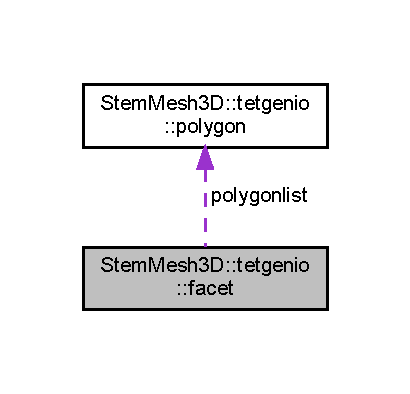
\includegraphics[width=197pt]{structStemMesh3D_1_1tetgenio_1_1facet__coll__graph}
\end{center}
\end{figure}
\subsection*{Public Attributes}
\begin{DoxyCompactItemize}
\item 
\mbox{\Hypertarget{structStemMesh3D_1_1tetgenio_1_1facet_a6dac27e73d3081d96b601fe4b4ace717}\label{structStemMesh3D_1_1tetgenio_1_1facet_a6dac27e73d3081d96b601fe4b4ace717}} 
\hyperlink{structStemMesh3D_1_1tetgenio_1_1polygon}{polygon} $\ast$ {\bfseries polygonlist}
\item 
\mbox{\Hypertarget{structStemMesh3D_1_1tetgenio_1_1facet_a025de49c723d8e9c45c924c9cfcc5d44}\label{structStemMesh3D_1_1tetgenio_1_1facet_a025de49c723d8e9c45c924c9cfcc5d44}} 
int {\bfseries numberofpolygons}
\item 
\mbox{\Hypertarget{structStemMesh3D_1_1tetgenio_1_1facet_a38a6b122d1623b1af93b60fa76a1da51}\label{structStemMesh3D_1_1tetgenio_1_1facet_a38a6b122d1623b1af93b60fa76a1da51}} 
R\+E\+AL $\ast$ {\bfseries holelist}
\item 
\mbox{\Hypertarget{structStemMesh3D_1_1tetgenio_1_1facet_afd2634c9adbec1599ced5386435dea6d}\label{structStemMesh3D_1_1tetgenio_1_1facet_afd2634c9adbec1599ced5386435dea6d}} 
int {\bfseries numberofholes}
\end{DoxyCompactItemize}


The documentation for this struct was generated from the following file\+:\begin{DoxyCompactItemize}
\item 
src/\+Mesh/\+Stem\+Mesh/tetgen.\+h\end{DoxyCompactItemize}

\hypertarget{classHArDCore3D_1_1Family}{}\section{H\+Ar\+D\+Core3D\+:\+:Family$<$ Basis\+Type $>$ Class Template Reference}
\label{classHArDCore3D_1_1Family}\index{H\+Ar\+D\+Core3\+D\+::\+Family$<$ Basis\+Type $>$@{H\+Ar\+D\+Core3\+D\+::\+Family$<$ Basis\+Type $>$}}


{\ttfamily \#include $<$basis.\+hpp$>$}

\subsection*{Public Types}
\begin{DoxyCompactItemize}
\item 
\mbox{\Hypertarget{classHArDCore3D_1_1Family_a2d87c9bf83c4dd0574dc399506d4870c}\label{classHArDCore3D_1_1Family_a2d87c9bf83c4dd0574dc399506d4870c}} 
typedef Basis\+Type\+::\+Function\+Value {\bfseries Function\+Value}
\item 
\mbox{\Hypertarget{classHArDCore3D_1_1Family_aa4c3dc501f6c7178d2ed5c797f9aefc1}\label{classHArDCore3D_1_1Family_aa4c3dc501f6c7178d2ed5c797f9aefc1}} 
typedef Basis\+Type\+::\+Gradient\+Value {\bfseries Gradient\+Value}
\item 
\mbox{\Hypertarget{classHArDCore3D_1_1Family_a7b53a354b3fad04c15ba0e35c46d3f51}\label{classHArDCore3D_1_1Family_a7b53a354b3fad04c15ba0e35c46d3f51}} 
typedef Vector\+Rd {\bfseries Curl\+Value}
\item 
\mbox{\Hypertarget{classHArDCore3D_1_1Family_a48cb296e638fde22922d3a583f6cf126}\label{classHArDCore3D_1_1Family_a48cb296e638fde22922d3a583f6cf126}} 
typedef double {\bfseries Divergence\+Value}
\item 
\mbox{\Hypertarget{classHArDCore3D_1_1Family_a9e16a6663722460eb003835c731bea9c}\label{classHArDCore3D_1_1Family_a9e16a6663722460eb003835c731bea9c}} 
typedef Basis\+Type\+::\+Geometric\+Support {\bfseries Geometric\+Support}
\end{DoxyCompactItemize}
\subsection*{Public Member Functions}
\begin{DoxyCompactItemize}
\item 
\hyperlink{classHArDCore3D_1_1Family_aa0576f3bfd8f5cdbdd863f147b646d15}{Family} (const Basis\+Type \&basis, const Eigen\+::\+Matrix\+Xd \&\hyperlink{classHArDCore3D_1_1Family_af056ff8a6cbf5c566c243290e72af217}{matrix})
\begin{DoxyCompactList}\small\item\em Constructor. \end{DoxyCompactList}\item 
\mbox{\Hypertarget{classHArDCore3D_1_1Family_aa71fa9b9c83346561fde4c764a1b2e72}\label{classHArDCore3D_1_1Family_aa71fa9b9c83346561fde4c764a1b2e72}} 
size\+\_\+t \hyperlink{classHArDCore3D_1_1Family_aa71fa9b9c83346561fde4c764a1b2e72}{dimension} () const
\begin{DoxyCompactList}\small\item\em Dimension of the family. This is actually the number of functions in the family, not necessarily linearly independent. \end{DoxyCompactList}\item 
\mbox{\Hypertarget{classHArDCore3D_1_1Family_a3616bf77a028e9e7638af28820370931}\label{classHArDCore3D_1_1Family_a3616bf77a028e9e7638af28820370931}} 
Function\+Value \hyperlink{classHArDCore3D_1_1Family_a3616bf77a028e9e7638af28820370931}{function} (size\+\_\+t i, const Vector\+Rd \&x) const
\begin{DoxyCompactList}\small\item\em Evaluate the i-\/th function at point x. \end{DoxyCompactList}\item 
\mbox{\Hypertarget{classHArDCore3D_1_1Family_a7e8e2733993bda1d5aff348d7d31cbcf}\label{classHArDCore3D_1_1Family_a7e8e2733993bda1d5aff348d7d31cbcf}} 
Gradient\+Value \hyperlink{classHArDCore3D_1_1Family_a7e8e2733993bda1d5aff348d7d31cbcf}{gradient} (size\+\_\+t i, const Vector\+Rd \&x) const
\begin{DoxyCompactList}\small\item\em Evaluate the gradient of the i-\/th function at point x. \end{DoxyCompactList}\item 
\mbox{\Hypertarget{classHArDCore3D_1_1Family_af5aac63dc865a440eb25c6b41b8d66d1}\label{classHArDCore3D_1_1Family_af5aac63dc865a440eb25c6b41b8d66d1}} 
Curl\+Value \hyperlink{classHArDCore3D_1_1Family_af5aac63dc865a440eb25c6b41b8d66d1}{curl} (size\+\_\+t i, const Vector\+Rd \&x) const
\begin{DoxyCompactList}\small\item\em Evaluate the curl of the i-\/th function at point x. \end{DoxyCompactList}\item 
\mbox{\Hypertarget{classHArDCore3D_1_1Family_a87cbacf4f0cf12e0c9cfe9afa2e40c29}\label{classHArDCore3D_1_1Family_a87cbacf4f0cf12e0c9cfe9afa2e40c29}} 
Divergence\+Value \hyperlink{classHArDCore3D_1_1Family_a87cbacf4f0cf12e0c9cfe9afa2e40c29}{divergence} (size\+\_\+t i, const Vector\+Rd \&x) const
\begin{DoxyCompactList}\small\item\em Evaluate the divergence of the i-\/th function at point x. \end{DoxyCompactList}\item 
\mbox{\Hypertarget{classHArDCore3D_1_1Family_af056ff8a6cbf5c566c243290e72af217}\label{classHArDCore3D_1_1Family_af056ff8a6cbf5c566c243290e72af217}} 
const Eigen\+::\+Matrix\+Xd \& \hyperlink{classHArDCore3D_1_1Family_af056ff8a6cbf5c566c243290e72af217}{matrix} () const
\begin{DoxyCompactList}\small\item\em Return the coefficient matrix. \end{DoxyCompactList}\item 
\mbox{\Hypertarget{classHArDCore3D_1_1Family_a7afd19f4c3c17b7ac8ed16115b0ffe1c}\label{classHArDCore3D_1_1Family_a7afd19f4c3c17b7ac8ed16115b0ffe1c}} 
const Basis\+Type \& \hyperlink{classHArDCore3D_1_1Family_a7afd19f4c3c17b7ac8ed16115b0ffe1c}{ancestor} () const
\begin{DoxyCompactList}\small\item\em Return the ancestor. \end{DoxyCompactList}\end{DoxyCompactItemize}
\subsection*{Static Public Attributes}
\begin{DoxyCompactItemize}
\item 
\mbox{\Hypertarget{classHArDCore3D_1_1Family_a78b538f422207983374190af40e1dfec}\label{classHArDCore3D_1_1Family_a78b538f422207983374190af40e1dfec}} 
static const Tensor\+RankE {\bfseries tensor\+Rank} = Basis\+Type\+::tensor\+Rank
\item 
\mbox{\Hypertarget{classHArDCore3D_1_1Family_ab00249d408f8228595197421aaf28ac6}\label{classHArDCore3D_1_1Family_ab00249d408f8228595197421aaf28ac6}} 
static const bool {\bfseries has\+Function} = Basis\+Type\+::has\+Function
\item 
\mbox{\Hypertarget{classHArDCore3D_1_1Family_a3fcb3b85e2f26f201e608b04bdf7f926}\label{classHArDCore3D_1_1Family_a3fcb3b85e2f26f201e608b04bdf7f926}} 
static const bool {\bfseries has\+Gradient} = Basis\+Type\+::has\+Gradient
\item 
\mbox{\Hypertarget{classHArDCore3D_1_1Family_a6c12f947e8ba8dedc3ac6809481249f0}\label{classHArDCore3D_1_1Family_a6c12f947e8ba8dedc3ac6809481249f0}} 
static const bool {\bfseries has\+Curl} = Basis\+Type\+::has\+Curl
\item 
\mbox{\Hypertarget{classHArDCore3D_1_1Family_ac905ca089d3f75eee5a4e655544b9223}\label{classHArDCore3D_1_1Family_ac905ca089d3f75eee5a4e655544b9223}} 
static const bool {\bfseries has\+Divergence} = Basis\+Type\+::has\+Divergence
\end{DoxyCompactItemize}


\subsection{Detailed Description}
\subsubsection*{template$<$typename Basis\+Type$>$\newline
class H\+Ar\+D\+Core3\+D\+::\+Family$<$ Basis\+Type $>$}

\hyperlink{classHArDCore3D_1_1Family}{Family} of functions expressed as linear combination of the functions of a given basis 

\subsection{Constructor \& Destructor Documentation}
\mbox{\Hypertarget{classHArDCore3D_1_1Family_aa0576f3bfd8f5cdbdd863f147b646d15}\label{classHArDCore3D_1_1Family_aa0576f3bfd8f5cdbdd863f147b646d15}} 
\index{H\+Ar\+D\+Core3\+D\+::\+Family@{H\+Ar\+D\+Core3\+D\+::\+Family}!Family@{Family}}
\index{Family@{Family}!H\+Ar\+D\+Core3\+D\+::\+Family@{H\+Ar\+D\+Core3\+D\+::\+Family}}
\subsubsection{\texorpdfstring{Family()}{Family()}}
{\footnotesize\ttfamily template$<$typename Basis\+Type$>$ \\
\hyperlink{classHArDCore3D_1_1Family}{H\+Ar\+D\+Core3\+D\+::\+Family}$<$ Basis\+Type $>$\+::\hyperlink{classHArDCore3D_1_1Family}{Family} (\begin{DoxyParamCaption}\item[{const Basis\+Type \&}]{basis,  }\item[{const Eigen\+::\+Matrix\+Xd \&}]{matrix }\end{DoxyParamCaption})\hspace{0.3cm}{\ttfamily [inline]}}



Constructor. 


\begin{DoxyParams}{Parameters}
{\em basis} & The basis in which the family is expressed \\
\hline
{\em matrix} & The coefficient matrix whose i-\/th line contains the coefficient of the expansion of the i-\/th function of the family in the basis \\
\hline
\end{DoxyParams}


The documentation for this class was generated from the following file\+:\begin{DoxyCompactItemize}
\item 
src/\+Common/basis.\+hpp\end{DoxyCompactItemize}

\hypertarget{classHArDCore3D_1_1GradientBasis}{}\section{H\+Ar\+D\+Core3D\+:\+:Gradient\+Basis$<$ Basis\+Type $>$ Class Template Reference}
\label{classHArDCore3D_1_1GradientBasis}\index{H\+Ar\+D\+Core3\+D\+::\+Gradient\+Basis$<$ Basis\+Type $>$@{H\+Ar\+D\+Core3\+D\+::\+Gradient\+Basis$<$ Basis\+Type $>$}}


{\ttfamily \#include $<$basis.\+hpp$>$}

\subsection*{Public Types}
\begin{DoxyCompactItemize}
\item 
\mbox{\Hypertarget{classHArDCore3D_1_1GradientBasis_afc6d347c3c4e36a9090cc91638bebfb4}\label{classHArDCore3D_1_1GradientBasis_afc6d347c3c4e36a9090cc91638bebfb4}} 
typedef Vector\+Rd {\bfseries Function\+Value}
\item 
\mbox{\Hypertarget{classHArDCore3D_1_1GradientBasis_a587b8fe3f498ae7ec7bb6ed4242958fa}\label{classHArDCore3D_1_1GradientBasis_a587b8fe3f498ae7ec7bb6ed4242958fa}} 
typedef Eigen\+::\+Matrix$<$ double, dimspace, dimspace $>$ {\bfseries Gradient\+Value}
\item 
\mbox{\Hypertarget{classHArDCore3D_1_1GradientBasis_ab588b4936d9f62067a8c2c5eb7572542}\label{classHArDCore3D_1_1GradientBasis_ab588b4936d9f62067a8c2c5eb7572542}} 
typedef Vector\+Rd {\bfseries Curl\+Value}
\item 
\mbox{\Hypertarget{classHArDCore3D_1_1GradientBasis_ab5c51bc59aeb61c403be368c4b4d4225}\label{classHArDCore3D_1_1GradientBasis_ab5c51bc59aeb61c403be368c4b4d4225}} 
typedef double {\bfseries Divergence\+Value}
\item 
\mbox{\Hypertarget{classHArDCore3D_1_1GradientBasis_adbd840e4cc2386bbf021731e359b60b0}\label{classHArDCore3D_1_1GradientBasis_adbd840e4cc2386bbf021731e359b60b0}} 
typedef Basis\+Type\+::\+Geometric\+Support {\bfseries Geometric\+Support}
\end{DoxyCompactItemize}
\subsection*{Public Member Functions}
\begin{DoxyCompactItemize}
\item 
\mbox{\Hypertarget{classHArDCore3D_1_1GradientBasis_af2fa9b4764b550f576aeba7e24e6c911}\label{classHArDCore3D_1_1GradientBasis_af2fa9b4764b550f576aeba7e24e6c911}} 
\hyperlink{classHArDCore3D_1_1GradientBasis_af2fa9b4764b550f576aeba7e24e6c911}{Gradient\+Basis} (const Basis\+Type \&basis)
\begin{DoxyCompactList}\small\item\em Constructor. \end{DoxyCompactList}\item 
\mbox{\Hypertarget{classHArDCore3D_1_1GradientBasis_abf5cc38208c346f4b6f6d5ca5d20d767}\label{classHArDCore3D_1_1GradientBasis_abf5cc38208c346f4b6f6d5ca5d20d767}} 
size\+\_\+t \hyperlink{classHArDCore3D_1_1GradientBasis_abf5cc38208c346f4b6f6d5ca5d20d767}{dimension} () const
\begin{DoxyCompactList}\small\item\em Compute the dimension of the basis. \end{DoxyCompactList}\item 
\mbox{\Hypertarget{classHArDCore3D_1_1GradientBasis_a21186eb9b6825da3867965bd2e046b23}\label{classHArDCore3D_1_1GradientBasis_a21186eb9b6825da3867965bd2e046b23}} 
Function\+Value \hyperlink{classHArDCore3D_1_1GradientBasis_a21186eb9b6825da3867965bd2e046b23}{function} (size\+\_\+t i, const Vector\+Rd \&x) const
\begin{DoxyCompactList}\small\item\em Evaluate the i-\/th basis function at point x. \end{DoxyCompactList}\end{DoxyCompactItemize}
\subsection*{Static Public Attributes}
\begin{DoxyCompactItemize}
\item 
\mbox{\Hypertarget{classHArDCore3D_1_1GradientBasis_ae15ea33e6d492df490f202061e73a5c7}\label{classHArDCore3D_1_1GradientBasis_ae15ea33e6d492df490f202061e73a5c7}} 
static const Tensor\+RankE {\bfseries tensor\+Rank} = Vector
\item 
\mbox{\Hypertarget{classHArDCore3D_1_1GradientBasis_ac70395c81f9bb7ec168fc77cb287f6b8}\label{classHArDCore3D_1_1GradientBasis_ac70395c81f9bb7ec168fc77cb287f6b8}} 
static const bool {\bfseries has\+Function} = true
\item 
\mbox{\Hypertarget{classHArDCore3D_1_1GradientBasis_a0c0ccb90014bf1b30726d5f8ac7f360d}\label{classHArDCore3D_1_1GradientBasis_a0c0ccb90014bf1b30726d5f8ac7f360d}} 
static const bool {\bfseries has\+Gradient} = false
\item 
\mbox{\Hypertarget{classHArDCore3D_1_1GradientBasis_ab2338daf54d3c72ca49f0cc665d35331}\label{classHArDCore3D_1_1GradientBasis_ab2338daf54d3c72ca49f0cc665d35331}} 
static const bool {\bfseries has\+Curl} = false
\item 
\mbox{\Hypertarget{classHArDCore3D_1_1GradientBasis_a3be6e64c5c36d83019fdfefd249a0f3d}\label{classHArDCore3D_1_1GradientBasis_a3be6e64c5c36d83019fdfefd249a0f3d}} 
static const bool {\bfseries has\+Divergence} = false
\end{DoxyCompactItemize}


\subsection{Detailed Description}
\subsubsection*{template$<$typename Basis\+Type$>$\newline
class H\+Ar\+D\+Core3\+D\+::\+Gradient\+Basis$<$ Basis\+Type $>$}

Basis for the space of gradients of polynomials. It assumes that the first function of the scalar basis is constant 

The documentation for this class was generated from the following file\+:\begin{DoxyCompactItemize}
\item 
src/\+Common/basis.\+hpp\end{DoxyCompactItemize}

\hypertarget{classHArDCore3D_1_1HHO__Diffusion}{}\doxysection{H\+Ar\+D\+Core3D\+::H\+H\+O\+\_\+\+Diffusion Class Reference}
\label{classHArDCore3D_1_1HHO__Diffusion}\index{HArDCore3D::HHO\_Diffusion@{HArDCore3D::HHO\_Diffusion}}


The \mbox{\hyperlink{classHArDCore3D_1_1HHO__Diffusion}{H\+H\+O\+\_\+\+Diffusion}} class provides tools to implement the H\+HO method for the diffusion problem.  




{\ttfamily \#include $<$H\+H\+O\+\_\+\+Diffusion.\+hpp$>$}

\doxysubsection*{Public Member Functions}
\begin{DoxyCompactItemize}
\item 
\mbox{\hyperlink{group__HHO__Diffusion_gaf93379edf8347fbe21240a2c88d0d5a2}{H\+H\+O\+\_\+\+Diffusion}} (\mbox{\hyperlink{classHArDCore3D_1_1HybridCore}{Hybrid\+Core}} \&hho, size\+\_\+t K, int L, Cell\+F\+Type$<$ Matrix\+Rd $>$ kappa, Cell\+F\+Type$<$ double $>$ source, \mbox{\hyperlink{classBoundaryConditions}{Boundary\+Conditions}} BC, \mbox{\hyperlink{group__Common_gaf7ef55817c2af72faaaa416170fba181}{F\+Type}}$<$ double $>$ exact\+\_\+solution, Cell\+F\+Type$<$ Vector\+Rd $>$ grad\+\_\+exact\+\_\+solution, std\+::string solver\+\_\+type, bool use\+\_\+threads, std\+::ostream \&output=std\+::cout)
\begin{DoxyCompactList}\small\item\em Constructor of the class. \end{DoxyCompactList}\item 
void \mbox{\hyperlink{group__HHO__Diffusion_ga82476d19a0312e0b370a1f6100d863d1}{assemble}} (\mbox{\hyperlink{classHArDCore3D_1_1HybridCore}{Hybrid\+Core}} \&hho)
\begin{DoxyCompactList}\small\item\em Assemble and solve the scheme. \end{DoxyCompactList}\item 
\mbox{\hyperlink{classHArDCore3D_1_1UVector}{U\+Vector}} {\bfseries solve} (\mbox{\hyperlink{classHArDCore3D_1_1HybridCore}{Hybrid\+Core}} \&hho)
\item 
double \mbox{\hyperlink{group__HHO__Diffusion_ga18588364740b7c9a8fc25213499eaadd}{Energy\+Norm}} (\mbox{\hyperlink{classHArDCore3D_1_1HybridCore}{Hybrid\+Core}} \&hho, const \mbox{\hyperlink{classHArDCore3D_1_1UVector}{U\+Vector}} Xh)
\begin{DoxyCompactList}\small\item\em Discrete energy norm (associated to the diffusion operator) of an hybrid function. \end{DoxyCompactList}\item 
double \mbox{\hyperlink{group__HHO__Diffusion_gaa2bb4d069026f1604d2899031d3642f1}{get\+\_\+assembly\+\_\+time}} () const
\begin{DoxyCompactList}\small\item\em cpu time to assemble the scheme \end{DoxyCompactList}\item 
double \mbox{\hyperlink{group__HHO__Diffusion_gadcad4a2ddc4f767a5cc59362c93adbc2}{get\+\_\+solving\+\_\+time}} () const
\begin{DoxyCompactList}\small\item\em cpu time to solve the scheme \end{DoxyCompactList}\item 
double \mbox{\hyperlink{group__HHO__Diffusion_ga91b1ec7d73685c4a1d49d671b4b69814}{get\+\_\+solving\+\_\+error}} () const
\begin{DoxyCompactList}\small\item\em residual after solving the scheme \end{DoxyCompactList}\item 
double \mbox{\hyperlink{group__HHO__Diffusion_ga00b3b186fb915242a805c7c53e323e6e}{get\+\_\+itime}} (size\+\_\+t idx) const
\begin{DoxyCompactList}\small\item\em various intermediate assembly times \end{DoxyCompactList}\item 
const size\+\_\+t \mbox{\hyperlink{group__HHO__Diffusion_ga6f5856e7137441c95a3495f2267facf3}{get\+\_\+nlocal\+\_\+cell\+\_\+dofs}} ()
\begin{DoxyCompactList}\small\item\em Number of D\+O\+Fs in each cell. \end{DoxyCompactList}\item 
const size\+\_\+t \mbox{\hyperlink{group__HHO__Diffusion_ga81f57d9aa97bcac14dbd4e0fc378bd46}{get\+\_\+nlocal\+\_\+face\+\_\+dofs}} ()
\begin{DoxyCompactList}\small\item\em Number of D\+O\+Fs on each face. \end{DoxyCompactList}\item 
const size\+\_\+t \mbox{\hyperlink{group__HHO__Diffusion_gabfc762c3cf9a0bbaf6f7d24512352e31}{get\+\_\+nhighorder\+\_\+dofs}} ()
\begin{DoxyCompactList}\small\item\em Number of D\+O\+Fs per cell for high-\/order (K+1) polynomials. \end{DoxyCompactList}\item 
const size\+\_\+t \mbox{\hyperlink{group__HHO__Diffusion_gadbbbcb3f31c94640fd926fb24cfc75c7}{get\+\_\+ntotal\+\_\+cell\+\_\+dofs}} ()
\begin{DoxyCompactList}\small\item\em Total number of cell D\+O\+Fs over the entire mesh. \end{DoxyCompactList}\item 
const size\+\_\+t \mbox{\hyperlink{group__HHO__Diffusion_ga22ff2e589a8b847354666ea2f9397b5b}{get\+\_\+ntotal\+\_\+face\+\_\+dofs}} ()
\begin{DoxyCompactList}\small\item\em Total number of face D\+O\+Fs over the entire mesh. \end{DoxyCompactList}\item 
const size\+\_\+t \mbox{\hyperlink{group__HHO__Diffusion_ga2e582a2d0dbd25ade261d160c32aa504}{get\+\_\+ndir\+\_\+face\+\_\+dofs}} ()
\begin{DoxyCompactList}\small\item\em Total number of face D\+O\+Fs for Dirichlet faces. \end{DoxyCompactList}\item 
const size\+\_\+t \mbox{\hyperlink{group__HHO__Diffusion_ga9564d2be867b683e002bb555d397ed09}{get\+\_\+ntotal\+\_\+dofs}} ()
\begin{DoxyCompactList}\small\item\em Total number of degrees of freedom over the entire mesh. \end{DoxyCompactList}\end{DoxyCompactItemize}


\doxysubsection{Detailed Description}
The \mbox{\hyperlink{classHArDCore3D_1_1HHO__Diffusion}{H\+H\+O\+\_\+\+Diffusion}} class provides tools to implement the H\+HO method for the diffusion problem. 

The documentation for this class was generated from the following file\+:\begin{DoxyCompactItemize}
\item 
Schemes/\+H\+H\+O-\/diffusion/H\+H\+O\+\_\+\+Diffusion.\+hpp\end{DoxyCompactItemize}

\hypertarget{classHArDCore3D_1_1HHO__LocVarDiff}{}\section{H\+Ar\+D\+Core3D\+:\+:H\+H\+O\+\_\+\+Loc\+Var\+Diff Class Reference}
\label{classHArDCore3D_1_1HHO__LocVarDiff}\index{H\+Ar\+D\+Core3\+D\+::\+H\+H\+O\+\_\+\+Loc\+Var\+Diff@{H\+Ar\+D\+Core3\+D\+::\+H\+H\+O\+\_\+\+Loc\+Var\+Diff}}


The \hyperlink{classHArDCore3D_1_1HHO__LocVarDiff}{H\+H\+O\+\_\+\+Loc\+Var\+Diff} class provides tools to implement the H\+HO method for the diffusion problem.  




{\ttfamily \#include $<$H\+H\+O\+\_\+\+Loc\+Var\+Diff.\+hpp$>$}

\subsection*{Public Types}
\begin{DoxyCompactItemize}
\item 
\mbox{\Hypertarget{classHArDCore3D_1_1HHO__LocVarDiff_a57cf83c67a9bcd71822a4ebdfbe0f0ce}\label{classHArDCore3D_1_1HHO__LocVarDiff_a57cf83c67a9bcd71822a4ebdfbe0f0ce}} 
using \hyperlink{classHArDCore3D_1_1HHO__LocVarDiff_a57cf83c67a9bcd71822a4ebdfbe0f0ce}{solution\+\_\+function\+\_\+type} = std\+::function$<$ double(double, double, double)$>$
\begin{DoxyCompactList}\small\item\em type for solution \end{DoxyCompactList}\item 
\mbox{\Hypertarget{classHArDCore3D_1_1HHO__LocVarDiff_a478a09a65f66428a614412e7d308ffcd}\label{classHArDCore3D_1_1HHO__LocVarDiff_a478a09a65f66428a614412e7d308ffcd}} 
using \hyperlink{classHArDCore3D_1_1HHO__LocVarDiff_a478a09a65f66428a614412e7d308ffcd}{source\+\_\+function\+\_\+type} = std\+::function$<$ double(double, double, double, \hyperlink{classHArDCore3D_1_1Cell}{Cell} $\ast$)$>$
\begin{DoxyCompactList}\small\item\em type for source \end{DoxyCompactList}\item 
\mbox{\Hypertarget{classHArDCore3D_1_1HHO__LocVarDiff_a13003c1e92aab2a21e3055e2fd7104f8}\label{classHArDCore3D_1_1HHO__LocVarDiff_a13003c1e92aab2a21e3055e2fd7104f8}} 
using \hyperlink{classHArDCore3D_1_1HHO__LocVarDiff_a13003c1e92aab2a21e3055e2fd7104f8}{grad\+\_\+function\+\_\+type} = std\+::function$<$ Eigen\+::\+Vector3d(double, double, double, \hyperlink{classHArDCore3D_1_1Cell}{Cell} $\ast$)$>$
\begin{DoxyCompactList}\small\item\em type for gradient \end{DoxyCompactList}\item 
\mbox{\Hypertarget{classHArDCore3D_1_1HHO__LocVarDiff_aba48f23cd9e46ab3b0d7d907e0990bd6}\label{classHArDCore3D_1_1HHO__LocVarDiff_aba48f23cd9e46ab3b0d7d907e0990bd6}} 
using \hyperlink{classHArDCore3D_1_1HHO__LocVarDiff_aba48f23cd9e46ab3b0d7d907e0990bd6}{tensor\+\_\+function\+\_\+type} = std\+::function$<$ Eigen\+::\+Matrix3d(double, double, double, \hyperlink{classHArDCore3D_1_1Cell}{Cell} $\ast$)$>$
\begin{DoxyCompactList}\small\item\em type for diffusion tensor \end{DoxyCompactList}\end{DoxyCompactItemize}
\subsection*{Public Member Functions}
\begin{DoxyCompactItemize}
\item 
\hyperlink{group__HHO__LocVarDiff_ga498c8ed6193d76926ca3f3627ed6cf11}{H\+H\+O\+\_\+\+Loc\+Var\+Diff} (\hyperlink{classHArDCore3D_1_1HHO__LocVarDiff_aba48f23cd9e46ab3b0d7d907e0990bd6}{tensor\+\_\+function\+\_\+type} kappa, size\+\_\+t deg\+\_\+kappa, \hyperlink{classHArDCore3D_1_1HHO__LocVarDiff_a478a09a65f66428a614412e7d308ffcd}{source\+\_\+function\+\_\+type} source, size\+\_\+t BC, \hyperlink{classHArDCore3D_1_1HHO__LocVarDiff_a57cf83c67a9bcd71822a4ebdfbe0f0ce}{solution\+\_\+function\+\_\+type} exact\+\_\+solution, \hyperlink{classHArDCore3D_1_1HHO__LocVarDiff_a13003c1e92aab2a21e3055e2fd7104f8}{grad\+\_\+function\+\_\+type} grad\+\_\+exact\+\_\+solution, std\+::string solver\+\_\+type)
\begin{DoxyCompactList}\small\item\em Constructor of the class. \end{DoxyCompactList}\item 
Eigen\+::\+Vector\+Xd \hyperlink{group__HHO__LocVarDiff_gab01c6aad8ad6264f67f866ec26c8055d}{solve} (\hyperlink{classHArDCore3D_1_1HybridCore}{Hybrid\+Core} \&hho)
\begin{DoxyCompactList}\small\item\em Assemble and solve the scheme. \end{DoxyCompactList}\item 
double \hyperlink{group__HHO__LocVarDiff_gab04749bad041c0ed9e91c54f262d42e1}{Energy\+Norm} (\hyperlink{classHArDCore3D_1_1HybridCore}{Hybrid\+Core} \&hho, const Eigen\+::\+Vector\+Xd Xh)
\begin{DoxyCompactList}\small\item\em Discrete energy norm (associated to the diffusion operator) of an hybrid function. \end{DoxyCompactList}\item 
double \hyperlink{group__HHO__LocVarDiff_ga4232eab7b9753215b506d5ce701c4f4f}{get\+\_\+assembly\+\_\+time} () const
\begin{DoxyCompactList}\small\item\em cpu time to assemble the scheme \end{DoxyCompactList}\item 
double \hyperlink{group__HHO__LocVarDiff_ga10971b2952ab54d336127a43f5ed9b29}{get\+\_\+solving\+\_\+time} () const
\begin{DoxyCompactList}\small\item\em cpu time to solve the scheme \end{DoxyCompactList}\item 
double \hyperlink{group__HHO__LocVarDiff_ga22542468093ee4e8e24d8c0a27946f8f}{get\+\_\+solving\+\_\+error} () const
\begin{DoxyCompactList}\small\item\em residual after solving the scheme \end{DoxyCompactList}\item 
double \hyperlink{group__HHO__LocVarDiff_gae66d0e79903e2ca077ff2515c20d7d2e}{get\+\_\+itime} (size\+\_\+t idx) const
\begin{DoxyCompactList}\small\item\em various intermediate assembly times \end{DoxyCompactList}\end{DoxyCompactItemize}


\subsection{Detailed Description}
The \hyperlink{classHArDCore3D_1_1HHO__LocVarDiff}{H\+H\+O\+\_\+\+Loc\+Var\+Diff} class provides tools to implement the H\+HO method for the diffusion problem. 

The documentation for this class was generated from the following file\+:\begin{DoxyCompactItemize}
\item 
Schemes/\+H\+H\+O-\/locvardiff/H\+H\+O\+\_\+\+Loc\+Var\+Diff.\+hpp\end{DoxyCompactItemize}

\hypertarget{classHArDCore3D_1_1HybridCore}{}\section{H\+Ar\+D\+Core3D\+:\+:Hybrid\+Core Class Reference}
\label{classHArDCore3D_1_1HybridCore}\index{H\+Ar\+D\+Core3\+D\+::\+Hybrid\+Core@{H\+Ar\+D\+Core3\+D\+::\+Hybrid\+Core}}


{\ttfamily \#include $<$hybridcore.\+hpp$>$}

\subsection*{Public Types}
\begin{DoxyCompactItemize}
\item 
\mbox{\Hypertarget{classHArDCore3D_1_1HybridCore_a9e760b418a3948b34114879f37086829}\label{classHArDCore3D_1_1HybridCore_a9e760b418a3948b34114879f37086829}} 
using \hyperlink{classHArDCore3D_1_1HybridCore_a9e760b418a3948b34114879f37086829}{cell\+\_\+basis\+\_\+type} = std\+::function$<$ double(double, double, double)$>$
\begin{DoxyCompactList}\small\item\em type for cell basis \end{DoxyCompactList}\item 
\mbox{\Hypertarget{classHArDCore3D_1_1HybridCore_ad4dd9ca67d6de59d7ea71c816d3d3e67}\label{classHArDCore3D_1_1HybridCore_ad4dd9ca67d6de59d7ea71c816d3d3e67}} 
using \hyperlink{classHArDCore3D_1_1HybridCore_ad4dd9ca67d6de59d7ea71c816d3d3e67}{cell\+\_\+gradient\+\_\+type} = std\+::function$<$ Eigen\+::\+Vector3d(double, double, double)$>$
\begin{DoxyCompactList}\small\item\em type for gradients of cell basis \end{DoxyCompactList}\item 
\mbox{\Hypertarget{classHArDCore3D_1_1HybridCore_ae0b0cdad94d3527d0b06e601c091cdad}\label{classHArDCore3D_1_1HybridCore_ae0b0cdad94d3527d0b06e601c091cdad}} 
using \hyperlink{classHArDCore3D_1_1HybridCore_ae0b0cdad94d3527d0b06e601c091cdad}{face\+\_\+basis\+\_\+type} = std\+::function$<$ double(double, double, double)$>$
\begin{DoxyCompactList}\small\item\em type for face basis \end{DoxyCompactList}\item 
\mbox{\Hypertarget{classHArDCore3D_1_1HybridCore_ae3e174245a6104913a2272e7fe96db46}\label{classHArDCore3D_1_1HybridCore_ae3e174245a6104913a2272e7fe96db46}} 
using \hyperlink{classHArDCore3D_1_1HybridCore_ae3e174245a6104913a2272e7fe96db46}{tensor\+\_\+function\+\_\+type} = std\+::function$<$ Eigen\+::\+Matrix3d(double, double, double)$>$
\begin{DoxyCompactList}\small\item\em type for 3D tensors basis \end{DoxyCompactList}\end{DoxyCompactItemize}
\subsection*{Public Member Functions}
\begin{DoxyCompactItemize}
\item 
\hyperlink{classHArDCore3D_1_1HybridCore_af4978b5ad1f20f152357e94ffa94bfa9}{Hybrid\+Core} (const \hyperlink{classHArDCore3D_1_1Mesh}{Mesh} $\ast$mesh\+\_\+ptr, const size\+\_\+t \hyperlink{group__HybridCore_ga5c5d20faf615bca6e170961a61464fb2}{K}, const size\+\_\+t \hyperlink{group__HybridCore_gae2bb060c207a888bf97a9d2a9626e1c0}{L}, const std\+::string choice\+\_\+basis=\char`\"{}Mon\char`\"{})
\begin{DoxyCompactList}\small\item\em Class constructor\+: initialises the data structure with the given mesh, and desired polynomial degrees of the basis functions. \end{DoxyCompactList}\item 
size\+\_\+t \hyperlink{classHArDCore3D_1_1HybridCore_aa2bdc59d150566e1b992058031509d2f}{dim\+\_\+\+Pcell} (const size\+\_\+t m) const
\begin{DoxyCompactList}\small\item\em Compute the size of the basis of 3-\/variate polynomials up to degree m. \end{DoxyCompactList}\item 
size\+\_\+t \hyperlink{classHArDCore3D_1_1HybridCore_a52d3a5aa6d681847e90c41d91abb360e}{dim\+\_\+\+Pface} (const size\+\_\+t m) const
\begin{DoxyCompactList}\small\item\em Compute the size of the basis of 1-\/variate polynomials up to degree m. \end{DoxyCompactList}\item 
const \hyperlink{classHArDCore3D_1_1HybridCore_a9e760b418a3948b34114879f37086829}{cell\+\_\+basis\+\_\+type} \& \hyperlink{classHArDCore3D_1_1HybridCore_aa7006921a9e212784abf688f63a855a0}{cell\+\_\+monomial} (size\+\_\+t iT, size\+\_\+t i) const
\begin{DoxyCompactList}\small\item\em Return a reference to the i\textquotesingle{}th monomial function of the cell iT. \end{DoxyCompactList}\item 
const \hyperlink{classHArDCore3D_1_1HybridCore_ae0b0cdad94d3527d0b06e601c091cdad}{face\+\_\+basis\+\_\+type} \& \hyperlink{classHArDCore3D_1_1HybridCore_a4544ebe6193ab5239fdca5381043c031}{face\+\_\+monomial} (size\+\_\+t iF, size\+\_\+t i) const
\begin{DoxyCompactList}\small\item\em Return a reference to the i\textquotesingle{}th monomial function of the face iF. \end{DoxyCompactList}\item 
const \hyperlink{classHArDCore3D_1_1HybridCore_a9e760b418a3948b34114879f37086829}{cell\+\_\+basis\+\_\+type} \& \hyperlink{classHArDCore3D_1_1HybridCore_a34242db07cc2b3c3b867d9e4580b634d}{cell\+\_\+basis} (size\+\_\+t iT, size\+\_\+t i) const
\begin{DoxyCompactList}\small\item\em Return a reference to the i\textquotesingle{}th basis function of the cell iT. \end{DoxyCompactList}\item 
const \hyperlink{classHArDCore3D_1_1HybridCore_ae0b0cdad94d3527d0b06e601c091cdad}{face\+\_\+basis\+\_\+type} \& \hyperlink{classHArDCore3D_1_1HybridCore_a7bacf0ebee651940baa7f04af5a47b65}{face\+\_\+basis} (size\+\_\+t iF, size\+\_\+t i) const
\begin{DoxyCompactList}\small\item\em Return a reference to the i\textquotesingle{}th basis function of the face iF. \end{DoxyCompactList}\item 
const \hyperlink{classHArDCore3D_1_1HybridCore_ad4dd9ca67d6de59d7ea71c816d3d3e67}{cell\+\_\+gradient\+\_\+type} \& \hyperlink{classHArDCore3D_1_1HybridCore_a0edb2fb02577f68744abb8a436381cf7}{cell\+\_\+monomials\+\_\+gradient} (size\+\_\+t iT, size\+\_\+t i) const
\begin{DoxyCompactList}\small\item\em Return a reference to the gradient of the i\textquotesingle{}th monomial function of the cell iT. \end{DoxyCompactList}\item 
const \hyperlink{classHArDCore3D_1_1HybridCore_ad4dd9ca67d6de59d7ea71c816d3d3e67}{cell\+\_\+gradient\+\_\+type} \& \hyperlink{classHArDCore3D_1_1HybridCore_a710fc23b914623b90a2699ab4291e539}{cell\+\_\+gradient} (size\+\_\+t iT, size\+\_\+t i) const
\begin{DoxyCompactList}\small\item\em Return a reference to the gradient of the i\textquotesingle{}th basis function of the celliT. \end{DoxyCompactList}\item 
\mbox{\Hypertarget{classHArDCore3D_1_1HybridCore_a02b46a742045262030431b73eb112f9c}\label{classHArDCore3D_1_1HybridCore_a02b46a742045262030431b73eb112f9c}} 
Eigen\+::\+Vector\+Xd \hyperlink{classHArDCore3D_1_1HybridCore_a02b46a742045262030431b73eb112f9c}{restr} (const Eigen\+::\+Vector\+Xd \&Xh, size\+\_\+t iT) const
\begin{DoxyCompactList}\small\item\em Extract from a global vector Xh of unknowns the unknowns corresponding to cell iT. \end{DoxyCompactList}\item 
\mbox{\Hypertarget{classHArDCore3D_1_1HybridCore_a6c2a3d4fde899dde50fda5d97eafdc07}\label{classHArDCore3D_1_1HybridCore_a6c2a3d4fde899dde50fda5d97eafdc07}} 
double \hyperlink{classHArDCore3D_1_1HybridCore_a6c2a3d4fde899dde50fda5d97eafdc07}{L2norm} (const Eigen\+::\+Vector\+Xd \&Xh) const
\begin{DoxyCompactList}\small\item\em Compute L2 norm of a discrete function (using cell values) \end{DoxyCompactList}\item 
\mbox{\Hypertarget{classHArDCore3D_1_1HybridCore_a5962007697ffc13367070f7c4bcbe875}\label{classHArDCore3D_1_1HybridCore_a5962007697ffc13367070f7c4bcbe875}} 
double \hyperlink{classHArDCore3D_1_1HybridCore_a5962007697ffc13367070f7c4bcbe875}{H1norm} (const Eigen\+::\+Vector\+Xd \&Xh) const
\begin{DoxyCompactList}\small\item\em Compute discrete H1 norm of a discrete function (using cell values) \end{DoxyCompactList}\item 
\mbox{\Hypertarget{classHArDCore3D_1_1HybridCore_a333758d69cc0cea9df7bd54042551504}\label{classHArDCore3D_1_1HybridCore_a333758d69cc0cea9df7bd54042551504}} 
double \hyperlink{classHArDCore3D_1_1HybridCore_a333758d69cc0cea9df7bd54042551504}{Linf\+\_\+face} (const Eigen\+::\+Vector\+Xd \&Xh) const
\begin{DoxyCompactList}\small\item\em Compute maximum of the coefficients on the face basis functions. \end{DoxyCompactList}\item 
{\footnotesize template$<$typename Function $>$ }\\Eigen\+::\+Vector\+Xd \hyperlink{group__HybridCore_gaa1c3baf0764f3f160759e0ffc8969dfb}{interpolate} (const Function \&f, size\+\_\+t doe) const
\begin{DoxyCompactList}\small\item\em Compute the interpolant in the discrete space of a continuous function. \end{DoxyCompactList}\item 
Eigen\+::\+Matrix\+Xd \hyperlink{classHArDCore3D_1_1HybridCore_aa5c203c11a661933930a33335b0e2479}{gram\+\_\+matrix} (const std\+::vector$<$ Eigen\+::\+Array\+Xd $>$ \&f\+\_\+quad, const std\+::vector$<$ Eigen\+::\+Array\+Xd $>$ \&g\+\_\+quad, const size\+\_\+t \&nrows, const size\+\_\+t \&ncols, const Quadrature\+Rule \&quad, const bool \&sym, std\+::vector$<$ double $>$ L2weight=\{\}) const
\item 
Eigen\+::\+Matrix\+Xd \hyperlink{classHArDCore3D_1_1HybridCore_a7403a7f6890fc8ffae6f8dc531c1b397}{gram\+\_\+matrix} (const std\+::vector$<$ Eigen\+::\+Array\+X\+Xd $>$ \&F\+\_\+quad, const std\+::vector$<$ Eigen\+::\+Array\+X\+Xd $>$ \&G\+\_\+quad, const size\+\_\+t \&nrows, const size\+\_\+t \&ncols, const Quadrature\+Rule \&quad, const bool \&sym, std\+::vector$<$ Eigen\+::\+Matrix3d $>$ L2\+Weight=\{\}) const
\begin{DoxyCompactList}\small\item\em Overloaded version of the previous one for vector-\/valued functions\+: the functions (F\+\_\+i) and (G\+\_\+j) are vector-\/valued functions. \end{DoxyCompactList}\item 
\mbox{\Hypertarget{classHArDCore3D_1_1HybridCore_a06825c5d156026d465a2798389aa952b}\label{classHArDCore3D_1_1HybridCore_a06825c5d156026d465a2798389aa952b}} 
Eigen\+::\+Vector\+Xd \hyperlink{classHArDCore3D_1_1HybridCore_a06825c5d156026d465a2798389aa952b}{compute\+\_\+weights} (size\+\_\+t iT) const
\begin{DoxyCompactList}\small\item\em Weights to compute cell unknowns from face unknowns when l=-\/1. \end{DoxyCompactList}\item 
const std\+::vector$<$ Eigen\+::\+Array\+Xd $>$ \hyperlink{classHArDCore3D_1_1HybridCore_af36cb92e3054b15c3b5b10fead49e925}{basis\+\_\+quad} (const std\+::string cellface, const size\+\_\+t i\+TF, const Quadrature\+Rule quad, const size\+\_\+t degree, const std\+::string type\+\_\+basis=\char`\"{}basis\char`\"{}) const
\begin{DoxyCompactList}\small\item\em Computes (cell or face) basis functions at the given quadrature nodes. \end{DoxyCompactList}\item 
const std\+::vector$<$ Eigen\+::\+Array\+X\+Xd $>$ \hyperlink{classHArDCore3D_1_1HybridCore_add794287f4bb49157a7b5f94a5ecb200}{grad\+\_\+basis\+\_\+quad} (const size\+\_\+t iT, const Quadrature\+Rule quad, const size\+\_\+t degree, const std\+::string type\+\_\+basis=\char`\"{}basis\char`\"{}) const
\begin{DoxyCompactList}\small\item\em Compute $(\nabla \phi_i)_{i\in I}$ at the given quadrature nodes, where $(\phi_i)_{i\in I}$ are the cell basis functions. \end{DoxyCompactList}\item 
\mbox{\Hypertarget{classHArDCore3D_1_1HybridCore_a19e0febebb2735a8cc7017873683b611}\label{classHArDCore3D_1_1HybridCore_a19e0febebb2735a8cc7017873683b611}} 
double \hyperlink{classHArDCore3D_1_1HybridCore_a19e0febebb2735a8cc7017873683b611}{evaluate\+\_\+in\+\_\+cell} (const Eigen\+::\+Vector\+Xd X\+TF, size\+\_\+t iT, double x, double y, double z) const
\begin{DoxyCompactList}\small\item\em Evaluates a discrete function in the cell iT at point (x,y,z) \end{DoxyCompactList}\item 
\mbox{\Hypertarget{classHArDCore3D_1_1HybridCore_a7364c571c3ecadb5a7025047478b3e40}\label{classHArDCore3D_1_1HybridCore_a7364c571c3ecadb5a7025047478b3e40}} 
double \hyperlink{classHArDCore3D_1_1HybridCore_a7364c571c3ecadb5a7025047478b3e40}{evaluate\+\_\+in\+\_\+face} (const Eigen\+::\+Vector\+Xd X\+TF, size\+\_\+t iF, double x, double y, double z) const
\begin{DoxyCompactList}\small\item\em Evaluates a discrete function on the face iF at point (x,y,z) \end{DoxyCompactList}\item 
const \hyperlink{classHArDCore3D_1_1Mesh}{Mesh} $\ast$ \hyperlink{group__HybridCore_gad4c32f117a1e67ec4a13dd9656c404e8}{get\+\_\+mesh\+\_\+ptr} () const
\begin{DoxyCompactList}\small\item\em returns a pointer to the mesh \end{DoxyCompactList}\item 
size\+\_\+t \hyperlink{group__HybridCore_ga5c5d20faf615bca6e170961a61464fb2}{K} () const
\begin{DoxyCompactList}\small\item\em polynomial degree of edge unknowns \end{DoxyCompactList}\item 
int \hyperlink{group__HybridCore_gae2bb060c207a888bf97a9d2a9626e1c0}{L} () const
\begin{DoxyCompactList}\small\item\em polynomial degree of cell unknowns \end{DoxyCompactList}\item 
int \hyperlink{group__HybridCore_ga907fd6e5325465e94acc67c831a14cdf}{Ldeg} () const
\begin{DoxyCompactList}\small\item\em usually equal to L, but put at 0 if L=-\/1 \end{DoxyCompactList}\item 
size\+\_\+t \hyperlink{group__HybridCore_ga804722e06e20a32477cd1ae41ee6f473}{ntotal\+\_\+dofs} () const
\begin{DoxyCompactList}\small\item\em Total number of degrees of freedom. \end{DoxyCompactList}\item 
size\+\_\+t \hyperlink{group__HybridCore_ga228678f9bf8057025f3c220e40cab209}{nlocal\+\_\+cell\+\_\+dofs} () const
\begin{DoxyCompactList}\small\item\em number of degrees of freedom in each cell (dimension of polynomial space) \end{DoxyCompactList}\item 
size\+\_\+t \hyperlink{group__HybridCore_gaae30736925e857cb467c3f5c75fdc97e}{ntotal\+\_\+cell\+\_\+dofs} () const
\begin{DoxyCompactList}\small\item\em total number of cell degrees of freedom \end{DoxyCompactList}\item 
size\+\_\+t \hyperlink{group__HybridCore_ga94fa97198237f40a378a384f3d072394}{nlocal\+\_\+face\+\_\+dofs} () const
\begin{DoxyCompactList}\small\item\em number of degrees of freedom on each face (dimension of polynomial space) \end{DoxyCompactList}\item 
size\+\_\+t \hyperlink{group__HybridCore_gab2e20ded434d1aacc44927934faabc1c}{ntotal\+\_\+face\+\_\+dofs} () const
\begin{DoxyCompactList}\small\item\em total number of face degrees of freedom \end{DoxyCompactList}\item 
size\+\_\+t \hyperlink{group__HybridCore_gaffef0ee3517c408e3d086956feb022bd}{ninternal\+\_\+face\+\_\+dofs} () const
\begin{DoxyCompactList}\small\item\em total number of face degrees of freedom for internal faces \end{DoxyCompactList}\item 
size\+\_\+t \hyperlink{group__HybridCore_gaddeb59cc8b5d89525e27b2dee22eb70f}{nboundary\+\_\+face\+\_\+dofs} () const
\begin{DoxyCompactList}\small\item\em total number of face degrees of freedom for boundary faces \end{DoxyCompactList}\item 
size\+\_\+t \hyperlink{group__HybridCore_ga07b815b769bba05753666f6bf900fdc5}{nhighorder\+\_\+dofs} () const
\begin{DoxyCompactList}\small\item\em total number of cell degrees of freedom with polynomials up to order k+1 \end{DoxyCompactList}\item 
size\+\_\+t \hyperlink{group__HybridCore_ga3b0fe217b02f8b2c132f6917e2ac9900}{ngradient\+\_\+dofs} () const
\begin{DoxyCompactList}\small\item\em total number of degrees of freedom for gradients \end{DoxyCompactList}\item 
{\footnotesize template$<$typename Function $>$ }\\void \hyperlink{group__HybridCore_gaca6e3380063a17fcb76276bc8c503d5b}{quadrature\+\_\+over\+\_\+cell} (const size\+\_\+t iT, const Function \&f) const
\begin{DoxyCompactList}\small\item\em To integrate a function over a cell. \end{DoxyCompactList}\item 
{\footnotesize template$<$typename Function $>$ }\\void \hyperlink{group__HybridCore_gabba9f8c9be9f2006a441304054b955c6}{quadrature\+\_\+over\+\_\+face} (const size\+\_\+t iF, const Function \&f) const
\begin{DoxyCompactList}\small\item\em To integrate a function over a face. \end{DoxyCompactList}\item 
{\footnotesize template$<$typename Function $>$ }\\double \hyperlink{group__HybridCore_ga1cb893746a3e8bdb80500be5c9382d96}{integrate\+\_\+over\+\_\+cell} (const size\+\_\+t iT, const Function \&f) const
\begin{DoxyCompactList}\small\item\em Integrates a function over a cell. Use with parcimony, expensive (re-\/compute quadratures) \end{DoxyCompactList}\item 
{\footnotesize template$<$typename Function $>$ }\\double \hyperlink{group__HybridCore_gacb6ad78c453a5a5ec6bc91d7a14e4c2a}{integrate\+\_\+over\+\_\+face} (const size\+\_\+t iF, const Function \&f) const
\begin{DoxyCompactList}\small\item\em Integrates a function over a face. Use with parcimony, expensive (re-\/compute quadratures) \end{DoxyCompactList}\item 
{\footnotesize template$<$typename Function $>$ }\\double \hyperlink{group__HybridCore_gad6aeaa4f65c67b92307c273254f539ed}{integrate\+\_\+over\+\_\+domain} (const Function \&f) const
\begin{DoxyCompactList}\small\item\em Integrates a function over the domaine. Use with parcimony, expensive (re-\/compute quadratures) \end{DoxyCompactList}\item 
Eigen\+::\+Vector\+Xd \hyperlink{classHArDCore3D_1_1HybridCore_a4e623d59fe09c23c4b714541e4aff5ea}{Vertex\+Values} (const Eigen\+::\+Vector\+Xd Xh, const std\+::string from\+\_\+dofs)
\begin{DoxyCompactList}\small\item\em From a hybrid function, computes a vector of values at the vertices of the mesh. \end{DoxyCompactList}\end{DoxyCompactItemize}


\subsection{Detailed Description}
The \hyperlink{classHArDCore3D_1_1HybridCore}{Hybrid\+Core} class provides convenient interfaces for performing integration over mesh cells and faces and handling polynomial basis functions\+The class also provides convenient interfaces for dealing with solutions to Hybrid High-\/\+Order schemes, such as the computation of integrals, norms and interpolants in the H\+HO space. 

\subsection{Constructor \& Destructor Documentation}
\mbox{\Hypertarget{classHArDCore3D_1_1HybridCore_af4978b5ad1f20f152357e94ffa94bfa9}\label{classHArDCore3D_1_1HybridCore_af4978b5ad1f20f152357e94ffa94bfa9}} 
\index{H\+Ar\+D\+Core3\+D\+::\+Hybrid\+Core@{H\+Ar\+D\+Core3\+D\+::\+Hybrid\+Core}!Hybrid\+Core@{Hybrid\+Core}}
\index{Hybrid\+Core@{Hybrid\+Core}!H\+Ar\+D\+Core3\+D\+::\+Hybrid\+Core@{H\+Ar\+D\+Core3\+D\+::\+Hybrid\+Core}}
\subsubsection{\texorpdfstring{Hybrid\+Core()}{HybridCore()}}
{\footnotesize\ttfamily Hybrid\+Core\+::\+Hybrid\+Core (\begin{DoxyParamCaption}\item[{const \hyperlink{classHArDCore3D_1_1Mesh}{Mesh} $\ast$}]{mesh\+\_\+ptr,  }\item[{const size\+\_\+t}]{K,  }\item[{const size\+\_\+t}]{L,  }\item[{const std\+::string}]{choice\+\_\+basis = {\ttfamily \char`\"{}Mon\char`\"{}} }\end{DoxyParamCaption})}



Class constructor\+: initialises the data structure with the given mesh, and desired polynomial degrees of the basis functions. 

The orthonormalisation comes at a cost in terms of manipulation of the basis functions. This should only be use when the polynomial degree is large and/or the cell is very distorted. However, in these cases, it can make a huge difference on the observed convergence rate. 
\begin{DoxyParams}{Parameters}
{\em mesh\+\_\+ptr} & A pointer to the loaded mesh \\
\hline
{\em K} & The degree of the face polynomials \\
\hline
{\em L} & The degree of the cell polynomials \\
\hline
{\em choice\+\_\+basis} & \char`\"{}\+Mon\char`\"{} for monomials basis, \char`\"{}\+O\+N\char`\"{} for orthonormalised basis. \\
\hline
\end{DoxyParams}


\subsection{Member Function Documentation}
\mbox{\Hypertarget{classHArDCore3D_1_1HybridCore_af36cb92e3054b15c3b5b10fead49e925}\label{classHArDCore3D_1_1HybridCore_af36cb92e3054b15c3b5b10fead49e925}} 
\index{H\+Ar\+D\+Core3\+D\+::\+Hybrid\+Core@{H\+Ar\+D\+Core3\+D\+::\+Hybrid\+Core}!basis\+\_\+quad@{basis\+\_\+quad}}
\index{basis\+\_\+quad@{basis\+\_\+quad}!H\+Ar\+D\+Core3\+D\+::\+Hybrid\+Core@{H\+Ar\+D\+Core3\+D\+::\+Hybrid\+Core}}
\subsubsection{\texorpdfstring{basis\+\_\+quad()}{basis\_quad()}}
{\footnotesize\ttfamily const std\+::vector$<$ Eigen\+::\+Array\+Xd $>$ Hybrid\+Core\+::basis\+\_\+quad (\begin{DoxyParamCaption}\item[{const std\+::string}]{cellface,  }\item[{const size\+\_\+t}]{i\+TF,  }\item[{const Quadrature\+Rule}]{quad,  }\item[{const size\+\_\+t}]{degree,  }\item[{const std\+::string}]{type\+\_\+basis = {\ttfamily \char`\"{}basis\char`\"{}} }\end{DoxyParamCaption}) const}



Computes (cell or face) basis functions at the given quadrature nodes. 

\begin{DoxyReturn}{Returns}
phi\+\_\+quad\mbox{[}i\mbox{]} = array listing the nbq (=nb of quadrature nodes) values of phi\+\_\+i at the quadrature nodes 
\end{DoxyReturn}

\begin{DoxyParams}{Parameters}
{\em cellface} & determines the type of basis function (cell or face) we want the values of \\
\hline
{\em i\+TF} & global index of the cell/face \\
\hline
{\em quad} & quadrature nodes and weights on the cell/face \\
\hline
{\em degree} & the maximum polynomial degree to consider \\
\hline
{\em type\+\_\+basis} & optional argument to determine if we want on the monomial, or the basis functions \\
\hline
\end{DoxyParams}
\mbox{\Hypertarget{classHArDCore3D_1_1HybridCore_a34242db07cc2b3c3b867d9e4580b634d}\label{classHArDCore3D_1_1HybridCore_a34242db07cc2b3c3b867d9e4580b634d}} 
\index{H\+Ar\+D\+Core3\+D\+::\+Hybrid\+Core@{H\+Ar\+D\+Core3\+D\+::\+Hybrid\+Core}!cell\+\_\+basis@{cell\+\_\+basis}}
\index{cell\+\_\+basis@{cell\+\_\+basis}!H\+Ar\+D\+Core3\+D\+::\+Hybrid\+Core@{H\+Ar\+D\+Core3\+D\+::\+Hybrid\+Core}}
\subsubsection{\texorpdfstring{cell\+\_\+basis()}{cell\_basis()}}
{\footnotesize\ttfamily const \hyperlink{classHArDCore3D_1_1HybridCore_a9e760b418a3948b34114879f37086829}{Hybrid\+Core\+::cell\+\_\+basis\+\_\+type} \& Hybrid\+Core\+::cell\+\_\+basis (\begin{DoxyParamCaption}\item[{size\+\_\+t}]{iT,  }\item[{size\+\_\+t}]{i }\end{DoxyParamCaption}) const}



Return a reference to the i\textquotesingle{}th basis function of the cell iT. 


\begin{DoxyParams}{Parameters}
{\em iT} & The global cell number of the cell \\
\hline
{\em i} & The index of the desired basis function \\
\hline
\end{DoxyParams}
\mbox{\Hypertarget{classHArDCore3D_1_1HybridCore_a710fc23b914623b90a2699ab4291e539}\label{classHArDCore3D_1_1HybridCore_a710fc23b914623b90a2699ab4291e539}} 
\index{H\+Ar\+D\+Core3\+D\+::\+Hybrid\+Core@{H\+Ar\+D\+Core3\+D\+::\+Hybrid\+Core}!cell\+\_\+gradient@{cell\+\_\+gradient}}
\index{cell\+\_\+gradient@{cell\+\_\+gradient}!H\+Ar\+D\+Core3\+D\+::\+Hybrid\+Core@{H\+Ar\+D\+Core3\+D\+::\+Hybrid\+Core}}
\subsubsection{\texorpdfstring{cell\+\_\+gradient()}{cell\_gradient()}}
{\footnotesize\ttfamily const \hyperlink{classHArDCore3D_1_1HybridCore_ad4dd9ca67d6de59d7ea71c816d3d3e67}{Hybrid\+Core\+::cell\+\_\+gradient\+\_\+type} \& Hybrid\+Core\+::cell\+\_\+gradient (\begin{DoxyParamCaption}\item[{size\+\_\+t}]{iT,  }\item[{size\+\_\+t}]{i }\end{DoxyParamCaption}) const}



Return a reference to the gradient of the i\textquotesingle{}th basis function of the celliT. 

Note that the gradient functions are indexed the same as the basis functions. In particular, this means that the first gradient function will always be identically zero, as it is the gradient of the constant basis function. 
\begin{DoxyParams}{Parameters}
{\em iT} & The global cell number of the cell \\
\hline
{\em i} & The index of the desired basis function \\
\hline
\end{DoxyParams}
\mbox{\Hypertarget{classHArDCore3D_1_1HybridCore_aa7006921a9e212784abf688f63a855a0}\label{classHArDCore3D_1_1HybridCore_aa7006921a9e212784abf688f63a855a0}} 
\index{H\+Ar\+D\+Core3\+D\+::\+Hybrid\+Core@{H\+Ar\+D\+Core3\+D\+::\+Hybrid\+Core}!cell\+\_\+monomial@{cell\+\_\+monomial}}
\index{cell\+\_\+monomial@{cell\+\_\+monomial}!H\+Ar\+D\+Core3\+D\+::\+Hybrid\+Core@{H\+Ar\+D\+Core3\+D\+::\+Hybrid\+Core}}
\subsubsection{\texorpdfstring{cell\+\_\+monomial()}{cell\_monomial()}}
{\footnotesize\ttfamily const \hyperlink{classHArDCore3D_1_1HybridCore_a9e760b418a3948b34114879f37086829}{Hybrid\+Core\+::cell\+\_\+basis\+\_\+type} \& Hybrid\+Core\+::cell\+\_\+monomial (\begin{DoxyParamCaption}\item[{size\+\_\+t}]{iT,  }\item[{size\+\_\+t}]{i }\end{DoxyParamCaption}) const}



Return a reference to the i\textquotesingle{}th monomial function of the cell iT. 


\begin{DoxyParams}{Parameters}
{\em iT} & The global cell number of the cell \\
\hline
{\em i} & The index of the desired monomial function \\
\hline
\end{DoxyParams}
\mbox{\Hypertarget{classHArDCore3D_1_1HybridCore_a0edb2fb02577f68744abb8a436381cf7}\label{classHArDCore3D_1_1HybridCore_a0edb2fb02577f68744abb8a436381cf7}} 
\index{H\+Ar\+D\+Core3\+D\+::\+Hybrid\+Core@{H\+Ar\+D\+Core3\+D\+::\+Hybrid\+Core}!cell\+\_\+monomials\+\_\+gradient@{cell\+\_\+monomials\+\_\+gradient}}
\index{cell\+\_\+monomials\+\_\+gradient@{cell\+\_\+monomials\+\_\+gradient}!H\+Ar\+D\+Core3\+D\+::\+Hybrid\+Core@{H\+Ar\+D\+Core3\+D\+::\+Hybrid\+Core}}
\subsubsection{\texorpdfstring{cell\+\_\+monomials\+\_\+gradient()}{cell\_monomials\_gradient()}}
{\footnotesize\ttfamily const \hyperlink{classHArDCore3D_1_1HybridCore_ad4dd9ca67d6de59d7ea71c816d3d3e67}{Hybrid\+Core\+::cell\+\_\+gradient\+\_\+type} \& Hybrid\+Core\+::cell\+\_\+monomials\+\_\+gradient (\begin{DoxyParamCaption}\item[{size\+\_\+t}]{iT,  }\item[{size\+\_\+t}]{i }\end{DoxyParamCaption}) const}



Return a reference to the gradient of the i\textquotesingle{}th monomial function of the cell iT. 

Note that the gradient functions are indexed the same as the monomial functions. In particular, this means that the first gradient function will always be identically zero, as it is the gradient of the constant monomial. 
\begin{DoxyParams}{Parameters}
{\em iT} & The global cell number of the cell \\
\hline
{\em i} & The index of the desired monomial function \\
\hline
\end{DoxyParams}
\mbox{\Hypertarget{classHArDCore3D_1_1HybridCore_aa2bdc59d150566e1b992058031509d2f}\label{classHArDCore3D_1_1HybridCore_aa2bdc59d150566e1b992058031509d2f}} 
\index{H\+Ar\+D\+Core3\+D\+::\+Hybrid\+Core@{H\+Ar\+D\+Core3\+D\+::\+Hybrid\+Core}!dim\+\_\+\+Pcell@{dim\+\_\+\+Pcell}}
\index{dim\+\_\+\+Pcell@{dim\+\_\+\+Pcell}!H\+Ar\+D\+Core3\+D\+::\+Hybrid\+Core@{H\+Ar\+D\+Core3\+D\+::\+Hybrid\+Core}}
\subsubsection{\texorpdfstring{dim\+\_\+\+Pcell()}{dim\_Pcell()}}
{\footnotesize\ttfamily size\+\_\+t Hybrid\+Core\+::dim\+\_\+\+Pcell (\begin{DoxyParamCaption}\item[{const size\+\_\+t}]{m }\end{DoxyParamCaption}) const}



Compute the size of the basis of 3-\/variate polynomials up to degree m. 


\begin{DoxyParams}{Parameters}
{\em m} & The maximum degree of the polynomial \\
\hline
\end{DoxyParams}
\mbox{\Hypertarget{classHArDCore3D_1_1HybridCore_a52d3a5aa6d681847e90c41d91abb360e}\label{classHArDCore3D_1_1HybridCore_a52d3a5aa6d681847e90c41d91abb360e}} 
\index{H\+Ar\+D\+Core3\+D\+::\+Hybrid\+Core@{H\+Ar\+D\+Core3\+D\+::\+Hybrid\+Core}!dim\+\_\+\+Pface@{dim\+\_\+\+Pface}}
\index{dim\+\_\+\+Pface@{dim\+\_\+\+Pface}!H\+Ar\+D\+Core3\+D\+::\+Hybrid\+Core@{H\+Ar\+D\+Core3\+D\+::\+Hybrid\+Core}}
\subsubsection{\texorpdfstring{dim\+\_\+\+Pface()}{dim\_Pface()}}
{\footnotesize\ttfamily size\+\_\+t Hybrid\+Core\+::dim\+\_\+\+Pface (\begin{DoxyParamCaption}\item[{const size\+\_\+t}]{m }\end{DoxyParamCaption}) const}



Compute the size of the basis of 1-\/variate polynomials up to degree m. 


\begin{DoxyParams}{Parameters}
{\em m} & The maximum degree of the polynomial \\
\hline
\end{DoxyParams}
\mbox{\Hypertarget{classHArDCore3D_1_1HybridCore_a7bacf0ebee651940baa7f04af5a47b65}\label{classHArDCore3D_1_1HybridCore_a7bacf0ebee651940baa7f04af5a47b65}} 
\index{H\+Ar\+D\+Core3\+D\+::\+Hybrid\+Core@{H\+Ar\+D\+Core3\+D\+::\+Hybrid\+Core}!face\+\_\+basis@{face\+\_\+basis}}
\index{face\+\_\+basis@{face\+\_\+basis}!H\+Ar\+D\+Core3\+D\+::\+Hybrid\+Core@{H\+Ar\+D\+Core3\+D\+::\+Hybrid\+Core}}
\subsubsection{\texorpdfstring{face\+\_\+basis()}{face\_basis()}}
{\footnotesize\ttfamily const \hyperlink{classHArDCore3D_1_1HybridCore_ae0b0cdad94d3527d0b06e601c091cdad}{Hybrid\+Core\+::face\+\_\+basis\+\_\+type} \& Hybrid\+Core\+::face\+\_\+basis (\begin{DoxyParamCaption}\item[{size\+\_\+t}]{iF,  }\item[{size\+\_\+t}]{i }\end{DoxyParamCaption}) const}



Return a reference to the i\textquotesingle{}th basis function of the face iF. 


\begin{DoxyParams}{Parameters}
{\em iF} & The global face number of the face \\
\hline
{\em i} & The index of the desired basis function \\
\hline
\end{DoxyParams}
\mbox{\Hypertarget{classHArDCore3D_1_1HybridCore_a4544ebe6193ab5239fdca5381043c031}\label{classHArDCore3D_1_1HybridCore_a4544ebe6193ab5239fdca5381043c031}} 
\index{H\+Ar\+D\+Core3\+D\+::\+Hybrid\+Core@{H\+Ar\+D\+Core3\+D\+::\+Hybrid\+Core}!face\+\_\+monomial@{face\+\_\+monomial}}
\index{face\+\_\+monomial@{face\+\_\+monomial}!H\+Ar\+D\+Core3\+D\+::\+Hybrid\+Core@{H\+Ar\+D\+Core3\+D\+::\+Hybrid\+Core}}
\subsubsection{\texorpdfstring{face\+\_\+monomial()}{face\_monomial()}}
{\footnotesize\ttfamily const \hyperlink{classHArDCore3D_1_1HybridCore_ae0b0cdad94d3527d0b06e601c091cdad}{Hybrid\+Core\+::face\+\_\+basis\+\_\+type} \& Hybrid\+Core\+::face\+\_\+monomial (\begin{DoxyParamCaption}\item[{size\+\_\+t}]{iF,  }\item[{size\+\_\+t}]{i }\end{DoxyParamCaption}) const}



Return a reference to the i\textquotesingle{}th monomial function of the face iF. 


\begin{DoxyParams}{Parameters}
{\em iF} & The global number of the face \\
\hline
{\em i} & The index of the desired monomial function \\
\hline
\end{DoxyParams}
\mbox{\Hypertarget{classHArDCore3D_1_1HybridCore_add794287f4bb49157a7b5f94a5ecb200}\label{classHArDCore3D_1_1HybridCore_add794287f4bb49157a7b5f94a5ecb200}} 
\index{H\+Ar\+D\+Core3\+D\+::\+Hybrid\+Core@{H\+Ar\+D\+Core3\+D\+::\+Hybrid\+Core}!grad\+\_\+basis\+\_\+quad@{grad\+\_\+basis\+\_\+quad}}
\index{grad\+\_\+basis\+\_\+quad@{grad\+\_\+basis\+\_\+quad}!H\+Ar\+D\+Core3\+D\+::\+Hybrid\+Core@{H\+Ar\+D\+Core3\+D\+::\+Hybrid\+Core}}
\subsubsection{\texorpdfstring{grad\+\_\+basis\+\_\+quad()}{grad\_basis\_quad()}}
{\footnotesize\ttfamily const std\+::vector$<$ Eigen\+::\+Array\+X\+Xd $>$ Hybrid\+Core\+::grad\+\_\+basis\+\_\+quad (\begin{DoxyParamCaption}\item[{const size\+\_\+t}]{iT,  }\item[{const Quadrature\+Rule}]{quad,  }\item[{const size\+\_\+t}]{degree,  }\item[{const std\+::string}]{type\+\_\+basis = {\ttfamily \char`\"{}basis\char`\"{}} }\end{DoxyParamCaption}) const}



Compute $(\nabla \phi_i)_{i\in I}$ at the given quadrature nodes, where $(\phi_i)_{i\in I}$ are the cell basis functions. 

\begin{DoxyReturn}{Returns}
dphi\+\_\+quad\mbox{[}i\mbox{]}\+: array of size 3$\ast$nbq (where nbq=nb of quadrature nodes), with each column being $\nabla \phi_i$ at the corresponding quadrature node 
\end{DoxyReturn}

\begin{DoxyParams}{Parameters}
{\em iT} & global index of the cell \\
\hline
{\em quad} & quadrature rules in the cell \\
\hline
{\em degree} & the maximum polynomial degree to consider \\
\hline
{\em type\+\_\+basis} & optional argument to determine if we want on the monomial, or the basis functions \\
\hline
\end{DoxyParams}
\mbox{\Hypertarget{classHArDCore3D_1_1HybridCore_aa5c203c11a661933930a33335b0e2479}\label{classHArDCore3D_1_1HybridCore_aa5c203c11a661933930a33335b0e2479}} 
\index{H\+Ar\+D\+Core3\+D\+::\+Hybrid\+Core@{H\+Ar\+D\+Core3\+D\+::\+Hybrid\+Core}!gram\+\_\+matrix@{gram\+\_\+matrix}}
\index{gram\+\_\+matrix@{gram\+\_\+matrix}!H\+Ar\+D\+Core3\+D\+::\+Hybrid\+Core@{H\+Ar\+D\+Core3\+D\+::\+Hybrid\+Core}}
\subsubsection{\texorpdfstring{gram\+\_\+matrix()}{gram\_matrix()}\hspace{0.1cm}{\footnotesize\ttfamily [1/2]}}
{\footnotesize\ttfamily Eigen\+::\+Matrix\+Xd Hybrid\+Core\+::gram\+\_\+matrix (\begin{DoxyParamCaption}\item[{const std\+::vector$<$ Eigen\+::\+Array\+Xd $>$ \&}]{f\+\_\+quad,  }\item[{const std\+::vector$<$ Eigen\+::\+Array\+Xd $>$ \&}]{g\+\_\+quad,  }\item[{const size\+\_\+t \&}]{nrows,  }\item[{const size\+\_\+t \&}]{ncols,  }\item[{const Quadrature\+Rule \&}]{quad,  }\item[{const bool \&}]{sym,  }\item[{std\+::vector$<$ double $>$}]{L2weight = {\ttfamily \{\}} }\end{DoxyParamCaption}) const}

Create the matrix of L2 products of two families (f\+\_\+i) and (g\+\_\+j) of functions (this is not really a Gram matrix, unless the two families are the same) \begin{DoxyReturn}{Returns}
The matrix $(\int f_i g_j)_{i=1\ldots nrows; j=1\ldots ncols}$ 
\end{DoxyReturn}

\begin{DoxyParams}{Parameters}
{\em f\+\_\+quad} & Values of functions (f1,f2,...) at the quadrature nodes \\
\hline
{\em g\+\_\+quad} & Values of functions (g1,g2,...) at the quadrature nodes \\
\hline
{\em nrows} & Number of rows of the matrix -\/ typically number of functions f\+\_\+i (but could be less) \\
\hline
{\em ncols} & Number of columns of the matrix -\/ typically number of functions g\+\_\+j (but could be less) \\
\hline
{\em quad} & Quadrature nodes for integration \\
\hline
{\em sym} & True if the matrix is pseudo-\/symmetric (that is, \#f$<$=\#g and f\+\_\+i=g\+\_\+i if i$<$=\#f) \\
\hline
{\em L2weight} & Optional weight for the L2 product. If provided, should be a std\+::vector$<$double$>$ of the weight at the quadrature nodes \\
\hline
\end{DoxyParams}
\mbox{\Hypertarget{classHArDCore3D_1_1HybridCore_a7403a7f6890fc8ffae6f8dc531c1b397}\label{classHArDCore3D_1_1HybridCore_a7403a7f6890fc8ffae6f8dc531c1b397}} 
\index{H\+Ar\+D\+Core3\+D\+::\+Hybrid\+Core@{H\+Ar\+D\+Core3\+D\+::\+Hybrid\+Core}!gram\+\_\+matrix@{gram\+\_\+matrix}}
\index{gram\+\_\+matrix@{gram\+\_\+matrix}!H\+Ar\+D\+Core3\+D\+::\+Hybrid\+Core@{H\+Ar\+D\+Core3\+D\+::\+Hybrid\+Core}}
\subsubsection{\texorpdfstring{gram\+\_\+matrix()}{gram\_matrix()}\hspace{0.1cm}{\footnotesize\ttfamily [2/2]}}
{\footnotesize\ttfamily Eigen\+::\+Matrix\+Xd Hybrid\+Core\+::gram\+\_\+matrix (\begin{DoxyParamCaption}\item[{const std\+::vector$<$ Eigen\+::\+Array\+X\+Xd $>$ \&}]{F\+\_\+quad,  }\item[{const std\+::vector$<$ Eigen\+::\+Array\+X\+Xd $>$ \&}]{G\+\_\+quad,  }\item[{const size\+\_\+t \&}]{nrows,  }\item[{const size\+\_\+t \&}]{ncols,  }\item[{const Quadrature\+Rule \&}]{quad,  }\item[{const bool \&}]{sym,  }\item[{std\+::vector$<$ Eigen\+::\+Matrix3d $>$}]{L2\+Weight = {\ttfamily \{\}} }\end{DoxyParamCaption}) const}



Overloaded version of the previous one for vector-\/valued functions\+: the functions (F\+\_\+i) and (G\+\_\+j) are vector-\/valued functions. 

\begin{DoxyReturn}{Returns}
The matrix $(\int F_i \cdot G_j)_{i=1\ldots nrows; j=1\ldots ncols}$ 
\end{DoxyReturn}

\begin{DoxyParams}{Parameters}
{\em F\+\_\+quad} & Values of functions (F1,F2,...) at the quadrature nodes \\
\hline
{\em G\+\_\+quad} & Values of functions (G1,G2,...) at the quadrature nodes \\
\hline
{\em nrows} & Number of rows of the matrix -\/ typically number of functions F\+\_\+i (but could be less) \\
\hline
{\em ncols} & Number of rows of the matrix -\/ typically number of functions G\+\_\+j (but could be less) \\
\hline
{\em quad} & Quadrature nodes for integration \\
\hline
{\em sym} & True if the matrix is pseudo-\/symmetric (that is, \#F$<$=\#G and F\+\_\+i=G\+\_\+i if i$<$=\#F) \\
\hline
{\em L2\+Weight} & Optional weight for the L2 product. If provided, should be a std\+::vector$<$\+Eigen\+::\+Matrix3d$>$ of the weight at the quadrature nodes \\
\hline
\end{DoxyParams}
\mbox{\Hypertarget{classHArDCore3D_1_1HybridCore_a4e623d59fe09c23c4b714541e4aff5ea}\label{classHArDCore3D_1_1HybridCore_a4e623d59fe09c23c4b714541e4aff5ea}} 
\index{H\+Ar\+D\+Core3\+D\+::\+Hybrid\+Core@{H\+Ar\+D\+Core3\+D\+::\+Hybrid\+Core}!Vertex\+Values@{Vertex\+Values}}
\index{Vertex\+Values@{Vertex\+Values}!H\+Ar\+D\+Core3\+D\+::\+Hybrid\+Core@{H\+Ar\+D\+Core3\+D\+::\+Hybrid\+Core}}
\subsubsection{\texorpdfstring{Vertex\+Values()}{VertexValues()}}
{\footnotesize\ttfamily Eigen\+::\+Vector\+Xd Hybrid\+Core\+::\+Vertex\+Values (\begin{DoxyParamCaption}\item[{const Eigen\+::\+Vector\+Xd}]{Xh,  }\item[{const std\+::string}]{from\+\_\+dofs }\end{DoxyParamCaption})}



From a hybrid function, computes a vector of values at the vertices of the mesh. 


\begin{DoxyParams}{Parameters}
{\em Xh} & hybrid function (cell and face polynomials) \\
\hline
{\em from\+\_\+dofs} & Type of unknowns to use\+: \char`\"{}cell\char`\"{} or \char`\"{}face\char`\"{} \\
\hline
\end{DoxyParams}


The documentation for this class was generated from the following files\+:\begin{DoxyCompactItemize}
\item 
src/\+Hybrid\+Core/hybridcore.\+hpp\item 
src/\+Hybrid\+Core/hybridcore.\+cpp\end{DoxyCompactItemize}

\hypertarget{classHArDCore3D_1_1LegendreGauss}{}\section{H\+Ar\+D\+Core3D\+:\+:Legendre\+Gauss Class Reference}
\label{classHArDCore3D_1_1LegendreGauss}\index{H\+Ar\+D\+Core3\+D\+::\+Legendre\+Gauss@{H\+Ar\+D\+Core3\+D\+::\+Legendre\+Gauss}}
\subsection*{Public Member Functions}
\begin{DoxyCompactItemize}
\item 
\mbox{\Hypertarget{classHArDCore3D_1_1LegendreGauss_a4df4c78f50b0116cb68151073a45e08a}\label{classHArDCore3D_1_1LegendreGauss_a4df4c78f50b0116cb68151073a45e08a}} 
{\bfseries Legendre\+Gauss} (size\+\_\+t doe)
\item 
\mbox{\Hypertarget{classHArDCore3D_1_1LegendreGauss_aa60072df54f7acc9bad7362e4d6f6f72}\label{classHArDCore3D_1_1LegendreGauss_aa60072df54f7acc9bad7362e4d6f6f72}} 
void {\bfseries sub\+\_\+rule\+\_\+01} ()
\item 
\mbox{\Hypertarget{classHArDCore3D_1_1LegendreGauss_a3b20f2cc13f96879fe731e3411e118cf}\label{classHArDCore3D_1_1LegendreGauss_a3b20f2cc13f96879fe731e3411e118cf}} 
void {\bfseries sub\+\_\+rule\+\_\+02} ()
\item 
\mbox{\Hypertarget{classHArDCore3D_1_1LegendreGauss_a0ee58d8688bfaaa7952cd7f70e06ad05}\label{classHArDCore3D_1_1LegendreGauss_a0ee58d8688bfaaa7952cd7f70e06ad05}} 
void {\bfseries sub\+\_\+rule\+\_\+03} ()
\item 
\mbox{\Hypertarget{classHArDCore3D_1_1LegendreGauss_a55751cb4eed2cd44b12fe7bcc505097a}\label{classHArDCore3D_1_1LegendreGauss_a55751cb4eed2cd44b12fe7bcc505097a}} 
void {\bfseries sub\+\_\+rule\+\_\+04} ()
\item 
\mbox{\Hypertarget{classHArDCore3D_1_1LegendreGauss_aa4e7cbaed5cea19a7490501e67bf728b}\label{classHArDCore3D_1_1LegendreGauss_aa4e7cbaed5cea19a7490501e67bf728b}} 
void {\bfseries sub\+\_\+rule\+\_\+05} ()
\item 
\mbox{\Hypertarget{classHArDCore3D_1_1LegendreGauss_aff68078ed4cdc77372609b56c3fcfc2a}\label{classHArDCore3D_1_1LegendreGauss_aff68078ed4cdc77372609b56c3fcfc2a}} 
void {\bfseries sub\+\_\+rule\+\_\+06} ()
\item 
\mbox{\Hypertarget{classHArDCore3D_1_1LegendreGauss_a70452a921cb1f1eb6e30d7436102ae01}\label{classHArDCore3D_1_1LegendreGauss_a70452a921cb1f1eb6e30d7436102ae01}} 
void {\bfseries sub\+\_\+rule\+\_\+07} ()
\item 
\mbox{\Hypertarget{classHArDCore3D_1_1LegendreGauss_a50b4238c7cade3272efe46641e1d2d3f}\label{classHArDCore3D_1_1LegendreGauss_a50b4238c7cade3272efe46641e1d2d3f}} 
void {\bfseries sub\+\_\+rule\+\_\+08} ()
\item 
\mbox{\Hypertarget{classHArDCore3D_1_1LegendreGauss_ae6a8077dd8cf9fc76ed1234b93691049}\label{classHArDCore3D_1_1LegendreGauss_ae6a8077dd8cf9fc76ed1234b93691049}} 
void {\bfseries sub\+\_\+rule\+\_\+09} ()
\item 
\mbox{\Hypertarget{classHArDCore3D_1_1LegendreGauss_aad37934da18110fd078f1950a575fd3d}\label{classHArDCore3D_1_1LegendreGauss_aad37934da18110fd078f1950a575fd3d}} 
void {\bfseries sub\+\_\+rule\+\_\+10} ()
\item 
\mbox{\Hypertarget{classHArDCore3D_1_1LegendreGauss_a6b7095506bd1d218c28f5778c6dea545}\label{classHArDCore3D_1_1LegendreGauss_a6b7095506bd1d218c28f5778c6dea545}} 
void {\bfseries sub\+\_\+rule\+\_\+11} ()
\item 
\mbox{\Hypertarget{classHArDCore3D_1_1LegendreGauss_a1251635135ab00a28e128a058288e440}\label{classHArDCore3D_1_1LegendreGauss_a1251635135ab00a28e128a058288e440}} 
size\+\_\+t {\bfseries npts} ()
\item 
\mbox{\Hypertarget{classHArDCore3D_1_1LegendreGauss_a2800eb7a7c2648b1edb77231ef42608a}\label{classHArDCore3D_1_1LegendreGauss_a2800eb7a7c2648b1edb77231ef42608a}} 
double {\bfseries wq} (size\+\_\+t i)
\item 
\mbox{\Hypertarget{classHArDCore3D_1_1LegendreGauss_aa10e032f4ea04323773b23177b4124ee}\label{classHArDCore3D_1_1LegendreGauss_aa10e032f4ea04323773b23177b4124ee}} 
double {\bfseries tq} (size\+\_\+t i)
\end{DoxyCompactItemize}


The documentation for this class was generated from the following files\+:\begin{DoxyCompactItemize}
\item 
src/\+Quadrature/quad1d.\+hpp\item 
src/\+Quadrature/quad1d.\+cpp\end{DoxyCompactItemize}

\hypertarget{classStemMesh3D_1_1tetgenmesh_1_1link}{}\doxysection{Stem\+Mesh3D\+::tetgenmesh\+::link Class Reference}
\label{classStemMesh3D_1_1tetgenmesh_1_1link}\index{StemMesh3D::tetgenmesh::link@{StemMesh3D::tetgenmesh::link}}


Inheritance diagram for Stem\+Mesh3D\+::tetgenmesh\+::link\+:\nopagebreak
\begin{figure}[H]
\begin{center}
\leavevmode
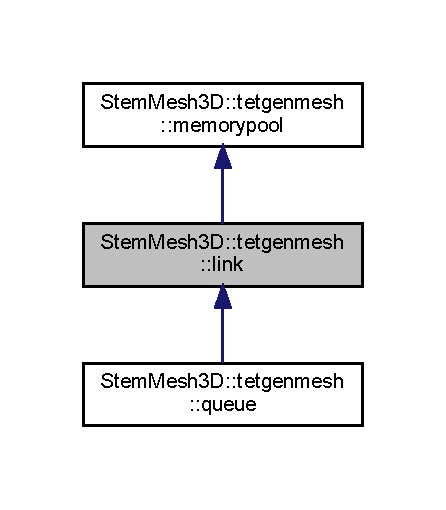
\includegraphics[width=214pt]{classStemMesh3D_1_1tetgenmesh_1_1link__inherit__graph}
\end{center}
\end{figure}


Collaboration diagram for Stem\+Mesh3D\+::tetgenmesh\+::link\+:\nopagebreak
\begin{figure}[H]
\begin{center}
\leavevmode
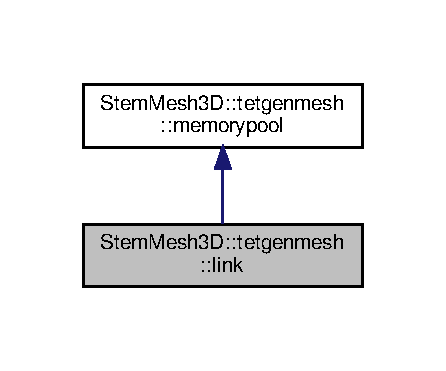
\includegraphics[width=214pt]{classStemMesh3D_1_1tetgenmesh_1_1link__coll__graph}
\end{center}
\end{figure}
\doxysubsection*{Public Member Functions}
\begin{DoxyCompactItemize}
\item 
\mbox{\Hypertarget{classStemMesh3D_1_1tetgenmesh_1_1link_a648d48615747a221bb63c57665576cf9}\label{classStemMesh3D_1_1tetgenmesh_1_1link_a648d48615747a221bb63c57665576cf9}} 
{\bfseries link} (int \+\_\+itembytes, compfunc \+\_\+comp, int itemcount)
\item 
\mbox{\Hypertarget{classStemMesh3D_1_1tetgenmesh_1_1link_a7297877a8b5aa71b367fe626e9c3edef}\label{classStemMesh3D_1_1tetgenmesh_1_1link_a7297877a8b5aa71b367fe626e9c3edef}} 
{\bfseries link} (char $\ast$str, int itemcount)
\item 
\mbox{\Hypertarget{classStemMesh3D_1_1tetgenmesh_1_1link_aeb16a9c9e31951fb584330f0c842d80f}\label{classStemMesh3D_1_1tetgenmesh_1_1link_aeb16a9c9e31951fb584330f0c842d80f}} 
void {\bfseries linkinit} (int \+\_\+itembytes, compfunc \+\_\+comp, int itemcount)
\item 
\mbox{\Hypertarget{classStemMesh3D_1_1tetgenmesh_1_1link_ad056d6320b70755e688dccc0973a20d6}\label{classStemMesh3D_1_1tetgenmesh_1_1link_ad056d6320b70755e688dccc0973a20d6}} 
void {\bfseries setcomp} (compfunc compf)
\item 
\mbox{\Hypertarget{classStemMesh3D_1_1tetgenmesh_1_1link_a0967a0ff7d437351e3464a5f970f6e6c}\label{classStemMesh3D_1_1tetgenmesh_1_1link_a0967a0ff7d437351e3464a5f970f6e6c}} 
void {\bfseries rewind} ()
\item 
\mbox{\Hypertarget{classStemMesh3D_1_1tetgenmesh_1_1link_ab0de3f0050a46c714526cb6c89452d23}\label{classStemMesh3D_1_1tetgenmesh_1_1link_ab0de3f0050a46c714526cb6c89452d23}} 
void {\bfseries goend} ()
\item 
\mbox{\Hypertarget{classStemMesh3D_1_1tetgenmesh_1_1link_a4a3f67cb1a170ad1e81168f68bac3c23}\label{classStemMesh3D_1_1tetgenmesh_1_1link_a4a3f67cb1a170ad1e81168f68bac3c23}} 
long {\bfseries len} ()
\item 
\mbox{\Hypertarget{classStemMesh3D_1_1tetgenmesh_1_1link_acb4400f07e0ca6053581eda225b4d316}\label{classStemMesh3D_1_1tetgenmesh_1_1link_acb4400f07e0ca6053581eda225b4d316}} 
void {\bfseries clear} ()
\item 
\mbox{\Hypertarget{classStemMesh3D_1_1tetgenmesh_1_1link_a649ad8523261dc9aa64f7e9d3e04b3f6}\label{classStemMesh3D_1_1tetgenmesh_1_1link_a649ad8523261dc9aa64f7e9d3e04b3f6}} 
bool {\bfseries move} (int numberofnodes)
\item 
\mbox{\Hypertarget{classStemMesh3D_1_1tetgenmesh_1_1link_af5b399749980807cfb693b999858a0b7}\label{classStemMesh3D_1_1tetgenmesh_1_1link_af5b399749980807cfb693b999858a0b7}} 
bool {\bfseries locate} (int pos)
\item 
\mbox{\Hypertarget{classStemMesh3D_1_1tetgenmesh_1_1link_ab7c22758f9e853b6eefab7c1da79cf6e}\label{classStemMesh3D_1_1tetgenmesh_1_1link_ab7c22758f9e853b6eefab7c1da79cf6e}} 
void $\ast$ {\bfseries add} (void $\ast$newitem)
\item 
\mbox{\Hypertarget{classStemMesh3D_1_1tetgenmesh_1_1link_abbc02eb09215252c666a5b5c22b1c1f4}\label{classStemMesh3D_1_1tetgenmesh_1_1link_abbc02eb09215252c666a5b5c22b1c1f4}} 
void $\ast$ {\bfseries insert} (int pos, void $\ast$insitem)
\item 
\mbox{\Hypertarget{classStemMesh3D_1_1tetgenmesh_1_1link_ab52cb30fa26c4ea3a2f727af555bb0ea}\label{classStemMesh3D_1_1tetgenmesh_1_1link_ab52cb30fa26c4ea3a2f727af555bb0ea}} 
void $\ast$ {\bfseries del} (void $\ast$delitem)
\item 
\mbox{\Hypertarget{classStemMesh3D_1_1tetgenmesh_1_1link_a4d7ce5d9689313b6414e9f33a33c0c0b}\label{classStemMesh3D_1_1tetgenmesh_1_1link_a4d7ce5d9689313b6414e9f33a33c0c0b}} 
void $\ast$ {\bfseries del} (int pos)
\item 
\mbox{\Hypertarget{classStemMesh3D_1_1tetgenmesh_1_1link_a1f45aa857c2f85dc91c4a6ba94093e21}\label{classStemMesh3D_1_1tetgenmesh_1_1link_a1f45aa857c2f85dc91c4a6ba94093e21}} 
void $\ast$ {\bfseries getitem} ()
\item 
\mbox{\Hypertarget{classStemMesh3D_1_1tetgenmesh_1_1link_a4d2a046dca330fdafc2c68e5478f32a3}\label{classStemMesh3D_1_1tetgenmesh_1_1link_a4d2a046dca330fdafc2c68e5478f32a3}} 
void $\ast$ {\bfseries getnitem} (int pos)
\item 
\mbox{\Hypertarget{classStemMesh3D_1_1tetgenmesh_1_1link_a6de0a510c48d6be0559a09f646627db3}\label{classStemMesh3D_1_1tetgenmesh_1_1link_a6de0a510c48d6be0559a09f646627db3}} 
int {\bfseries hasitem} (void $\ast$checkitem)
\end{DoxyCompactItemize}
\doxysubsection*{Public Attributes}
\begin{DoxyCompactItemize}
\item 
\mbox{\Hypertarget{classStemMesh3D_1_1tetgenmesh_1_1link_a53b1ba6a5730bdf9722bc03bae7b3c8c}\label{classStemMesh3D_1_1tetgenmesh_1_1link_a53b1ba6a5730bdf9722bc03bae7b3c8c}} 
void $\ast$$\ast$ {\bfseries head}
\item 
\mbox{\Hypertarget{classStemMesh3D_1_1tetgenmesh_1_1link_a484da4ef25442b2ac63735ecbce3cea6}\label{classStemMesh3D_1_1tetgenmesh_1_1link_a484da4ef25442b2ac63735ecbce3cea6}} 
void $\ast$$\ast$ {\bfseries tail}
\item 
\mbox{\Hypertarget{classStemMesh3D_1_1tetgenmesh_1_1link_a363ae663ff1b1c3cd16dc1c1904f1373}\label{classStemMesh3D_1_1tetgenmesh_1_1link_a363ae663ff1b1c3cd16dc1c1904f1373}} 
void $\ast$ {\bfseries nextlinkitem}
\item 
\mbox{\Hypertarget{classStemMesh3D_1_1tetgenmesh_1_1link_a40b91c0d17c55e01f2808309425ba879}\label{classStemMesh3D_1_1tetgenmesh_1_1link_a40b91c0d17c55e01f2808309425ba879}} 
int {\bfseries linkitembytes}
\item 
\mbox{\Hypertarget{classStemMesh3D_1_1tetgenmesh_1_1link_aaa3c5b3544876a23f40cd0e1995e0cd5}\label{classStemMesh3D_1_1tetgenmesh_1_1link_aaa3c5b3544876a23f40cd0e1995e0cd5}} 
int {\bfseries linkitems}
\item 
\mbox{\Hypertarget{classStemMesh3D_1_1tetgenmesh_1_1link_abba8c83d0ee67ffa4f486e6dee9e5ffe}\label{classStemMesh3D_1_1tetgenmesh_1_1link_abba8c83d0ee67ffa4f486e6dee9e5ffe}} 
int {\bfseries curpos}
\item 
\mbox{\Hypertarget{classStemMesh3D_1_1tetgenmesh_1_1link_a0a4de95c2ededd5ec762cbc6c73ceb0c}\label{classStemMesh3D_1_1tetgenmesh_1_1link_a0a4de95c2ededd5ec762cbc6c73ceb0c}} 
compfunc {\bfseries comp}
\end{DoxyCompactItemize}


The documentation for this class was generated from the following file\+:\begin{DoxyCompactItemize}
\item 
src/\+Mesh/\+Stem\+Mesh/tetgen.\+h\end{DoxyCompactItemize}

\hypertarget{classStemMesh3D_1_1tetgenmesh_1_1list}{}\section{Stem\+Mesh3D\+:\+:tetgenmesh\+:\+:list Class Reference}
\label{classStemMesh3D_1_1tetgenmesh_1_1list}\index{Stem\+Mesh3\+D\+::tetgenmesh\+::list@{Stem\+Mesh3\+D\+::tetgenmesh\+::list}}
\subsection*{Public Member Functions}
\begin{DoxyCompactItemize}
\item 
\mbox{\Hypertarget{classStemMesh3D_1_1tetgenmesh_1_1list_a6f96ef4612ca0960b99f31d575d7e20f}\label{classStemMesh3D_1_1tetgenmesh_1_1list_a6f96ef4612ca0960b99f31d575d7e20f}} 
{\bfseries list} (int itbytes, compfunc pcomp, int mitems=256, int exsize=128)
\item 
\mbox{\Hypertarget{classStemMesh3D_1_1tetgenmesh_1_1list_a7ef2cba610b899349de44c375bdd1aa9}\label{classStemMesh3D_1_1tetgenmesh_1_1list_a7ef2cba610b899349de44c375bdd1aa9}} 
{\bfseries list} (char $\ast$str, int mitems=256, int exsize=128)
\item 
\mbox{\Hypertarget{classStemMesh3D_1_1tetgenmesh_1_1list_a78c08c05ee1c591bf88030241c808de2}\label{classStemMesh3D_1_1tetgenmesh_1_1list_a78c08c05ee1c591bf88030241c808de2}} 
void $\ast$ {\bfseries operator\mbox{[}$\,$\mbox{]}} (int i)
\item 
\mbox{\Hypertarget{classStemMesh3D_1_1tetgenmesh_1_1list_afc6efbc41dc8ca6f574ff51a01c22a0c}\label{classStemMesh3D_1_1tetgenmesh_1_1list_afc6efbc41dc8ca6f574ff51a01c22a0c}} 
void {\bfseries listinit} (int itbytes, compfunc pcomp, int mitems, int exsize)
\item 
\mbox{\Hypertarget{classStemMesh3D_1_1tetgenmesh_1_1list_af4381844c6ba1d6c1d810072e22106dc}\label{classStemMesh3D_1_1tetgenmesh_1_1list_af4381844c6ba1d6c1d810072e22106dc}} 
void {\bfseries setcomp} (compfunc compf)
\item 
\mbox{\Hypertarget{classStemMesh3D_1_1tetgenmesh_1_1list_a64e7fcc6bccdd2f4d53238298cfeb36f}\label{classStemMesh3D_1_1tetgenmesh_1_1list_a64e7fcc6bccdd2f4d53238298cfeb36f}} 
void {\bfseries clear} ()
\item 
\mbox{\Hypertarget{classStemMesh3D_1_1tetgenmesh_1_1list_ad42545c80b7b4de8c1185b3d8aa32f28}\label{classStemMesh3D_1_1tetgenmesh_1_1list_ad42545c80b7b4de8c1185b3d8aa32f28}} 
int {\bfseries len} ()
\item 
\mbox{\Hypertarget{classStemMesh3D_1_1tetgenmesh_1_1list_ae0a778f7a04f4cd2acdddc31e1d9fdb6}\label{classStemMesh3D_1_1tetgenmesh_1_1list_ae0a778f7a04f4cd2acdddc31e1d9fdb6}} 
void $\ast$ {\bfseries append} (void $\ast$appitem)
\item 
\mbox{\Hypertarget{classStemMesh3D_1_1tetgenmesh_1_1list_af2077040e9603281d13e10cad0d4d460}\label{classStemMesh3D_1_1tetgenmesh_1_1list_af2077040e9603281d13e10cad0d4d460}} 
void $\ast$ {\bfseries insert} (int pos, void $\ast$insitem)
\item 
\mbox{\Hypertarget{classStemMesh3D_1_1tetgenmesh_1_1list_a79e32b1e5e2444587424465285845b7e}\label{classStemMesh3D_1_1tetgenmesh_1_1list_a79e32b1e5e2444587424465285845b7e}} 
void {\bfseries del} (int pos)
\item 
\mbox{\Hypertarget{classStemMesh3D_1_1tetgenmesh_1_1list_a61627a6b3c71c4bcc3c1a861bbe60934}\label{classStemMesh3D_1_1tetgenmesh_1_1list_a61627a6b3c71c4bcc3c1a861bbe60934}} 
int {\bfseries hasitem} (void $\ast$checkitem)
\item 
\mbox{\Hypertarget{classStemMesh3D_1_1tetgenmesh_1_1list_a53f6fadbf4dcda8ef92d1a336058f63a}\label{classStemMesh3D_1_1tetgenmesh_1_1list_a53f6fadbf4dcda8ef92d1a336058f63a}} 
int {\bfseries remove} (void $\ast$remitem)
\item 
\mbox{\Hypertarget{classStemMesh3D_1_1tetgenmesh_1_1list_ad335a57a47137dc1a13beeb175ab3fb5}\label{classStemMesh3D_1_1tetgenmesh_1_1list_ad335a57a47137dc1a13beeb175ab3fb5}} 
void {\bfseries sort} ()
\end{DoxyCompactItemize}
\subsection*{Public Attributes}
\begin{DoxyCompactItemize}
\item 
\mbox{\Hypertarget{classStemMesh3D_1_1tetgenmesh_1_1list_a3f162875d9b3437b6fc7062018a45b48}\label{classStemMesh3D_1_1tetgenmesh_1_1list_a3f162875d9b3437b6fc7062018a45b48}} 
char $\ast$ {\bfseries base}
\item 
\mbox{\Hypertarget{classStemMesh3D_1_1tetgenmesh_1_1list_abe7daba7fd6723310561defc74f8c759}\label{classStemMesh3D_1_1tetgenmesh_1_1list_abe7daba7fd6723310561defc74f8c759}} 
int {\bfseries itembytes}
\item 
\mbox{\Hypertarget{classStemMesh3D_1_1tetgenmesh_1_1list_afd78e49c41e0a166faf40d85379afec6}\label{classStemMesh3D_1_1tetgenmesh_1_1list_afd78e49c41e0a166faf40d85379afec6}} 
int {\bfseries items}
\item 
\mbox{\Hypertarget{classStemMesh3D_1_1tetgenmesh_1_1list_a6bc2578cc7332a5e92f8c21248d305be}\label{classStemMesh3D_1_1tetgenmesh_1_1list_a6bc2578cc7332a5e92f8c21248d305be}} 
int {\bfseries maxitems}
\item 
\mbox{\Hypertarget{classStemMesh3D_1_1tetgenmesh_1_1list_a62e4d76d5343eae99ac1330adeb7928a}\label{classStemMesh3D_1_1tetgenmesh_1_1list_a62e4d76d5343eae99ac1330adeb7928a}} 
int {\bfseries expandsize}
\item 
\mbox{\Hypertarget{classStemMesh3D_1_1tetgenmesh_1_1list_aa3733f509f961b4d8f1dcaec183eb862}\label{classStemMesh3D_1_1tetgenmesh_1_1list_aa3733f509f961b4d8f1dcaec183eb862}} 
compfunc {\bfseries comp}
\end{DoxyCompactItemize}


The documentation for this class was generated from the following file\+:\begin{DoxyCompactItemize}
\item 
src/\+Mesh/\+Stem\+Mesh/tetgen.\+h\end{DoxyCompactItemize}

\hypertarget{classStemMesh3D_1_1tetgenmesh_1_1memorypool}{}\doxysection{Stem\+Mesh3D\+::tetgenmesh\+::memorypool Class Reference}
\label{classStemMesh3D_1_1tetgenmesh_1_1memorypool}\index{StemMesh3D::tetgenmesh::memorypool@{StemMesh3D::tetgenmesh::memorypool}}


Inheritance diagram for Stem\+Mesh3D\+::tetgenmesh\+::memorypool\+:\nopagebreak
\begin{figure}[H]
\begin{center}
\leavevmode
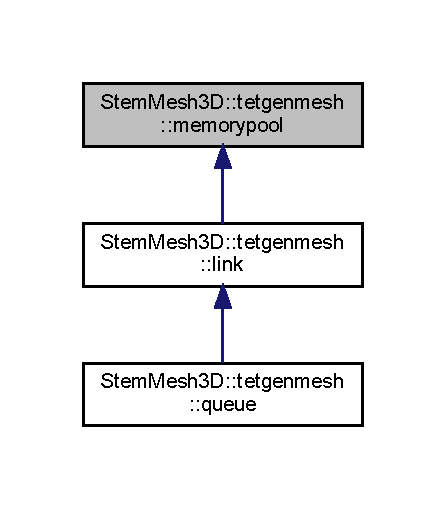
\includegraphics[width=214pt]{classStemMesh3D_1_1tetgenmesh_1_1memorypool__inherit__graph}
\end{center}
\end{figure}
\doxysubsection*{Public Member Functions}
\begin{DoxyCompactItemize}
\item 
\mbox{\Hypertarget{classStemMesh3D_1_1tetgenmesh_1_1memorypool_a4edfe23323ae05ce0b376b10531b0572}\label{classStemMesh3D_1_1tetgenmesh_1_1memorypool_a4edfe23323ae05ce0b376b10531b0572}} 
{\bfseries memorypool} (int, int, enum wordtype, int)
\item 
\mbox{\Hypertarget{classStemMesh3D_1_1tetgenmesh_1_1memorypool_a3fbe69f0a443d8caadb06d94039190f5}\label{classStemMesh3D_1_1tetgenmesh_1_1memorypool_a3fbe69f0a443d8caadb06d94039190f5}} 
void {\bfseries poolinit} (int, int, enum wordtype, int)
\item 
\mbox{\Hypertarget{classStemMesh3D_1_1tetgenmesh_1_1memorypool_aebe59eb1b11d410efb54c11ddb2c1862}\label{classStemMesh3D_1_1tetgenmesh_1_1memorypool_aebe59eb1b11d410efb54c11ddb2c1862}} 
void {\bfseries restart} ()
\item 
\mbox{\Hypertarget{classStemMesh3D_1_1tetgenmesh_1_1memorypool_a265b7943378133b12de36113154c4891}\label{classStemMesh3D_1_1tetgenmesh_1_1memorypool_a265b7943378133b12de36113154c4891}} 
void $\ast$ {\bfseries alloc} ()
\item 
\mbox{\Hypertarget{classStemMesh3D_1_1tetgenmesh_1_1memorypool_afce1801091914bed0425883d64aa8790}\label{classStemMesh3D_1_1tetgenmesh_1_1memorypool_afce1801091914bed0425883d64aa8790}} 
void {\bfseries dealloc} (void $\ast$)
\item 
\mbox{\Hypertarget{classStemMesh3D_1_1tetgenmesh_1_1memorypool_ad84cb536db64a5b7e13c6837b39861ce}\label{classStemMesh3D_1_1tetgenmesh_1_1memorypool_ad84cb536db64a5b7e13c6837b39861ce}} 
void {\bfseries traversalinit} ()
\item 
\mbox{\Hypertarget{classStemMesh3D_1_1tetgenmesh_1_1memorypool_a6ef43c3a4774c394fccf18dbe7a3a8f7}\label{classStemMesh3D_1_1tetgenmesh_1_1memorypool_a6ef43c3a4774c394fccf18dbe7a3a8f7}} 
void $\ast$ {\bfseries traverse} ()
\end{DoxyCompactItemize}
\doxysubsection*{Public Attributes}
\begin{DoxyCompactItemize}
\item 
\mbox{\Hypertarget{classStemMesh3D_1_1tetgenmesh_1_1memorypool_aa7e6630b0e234347c9ee525f24227f06}\label{classStemMesh3D_1_1tetgenmesh_1_1memorypool_aa7e6630b0e234347c9ee525f24227f06}} 
void $\ast$$\ast$ {\bfseries firstblock}
\item 
\mbox{\Hypertarget{classStemMesh3D_1_1tetgenmesh_1_1memorypool_ab9e43ba581b012f7856c6d63198e7310}\label{classStemMesh3D_1_1tetgenmesh_1_1memorypool_ab9e43ba581b012f7856c6d63198e7310}} 
void $\ast$$\ast$ {\bfseries nowblock}
\item 
\mbox{\Hypertarget{classStemMesh3D_1_1tetgenmesh_1_1memorypool_afa972dbff2871669a071bb45c30ebc74}\label{classStemMesh3D_1_1tetgenmesh_1_1memorypool_afa972dbff2871669a071bb45c30ebc74}} 
void $\ast$ {\bfseries nextitem}
\item 
\mbox{\Hypertarget{classStemMesh3D_1_1tetgenmesh_1_1memorypool_a10332959f6d92902daf2ae9ffb9622ae}\label{classStemMesh3D_1_1tetgenmesh_1_1memorypool_a10332959f6d92902daf2ae9ffb9622ae}} 
void $\ast$ {\bfseries deaditemstack}
\item 
\mbox{\Hypertarget{classStemMesh3D_1_1tetgenmesh_1_1memorypool_ab560cfa6887de01c438f7f402db2ecd3}\label{classStemMesh3D_1_1tetgenmesh_1_1memorypool_ab560cfa6887de01c438f7f402db2ecd3}} 
void $\ast$$\ast$ {\bfseries pathblock}
\item 
\mbox{\Hypertarget{classStemMesh3D_1_1tetgenmesh_1_1memorypool_acfbd44470b1399397b17611e3c3c1bec}\label{classStemMesh3D_1_1tetgenmesh_1_1memorypool_acfbd44470b1399397b17611e3c3c1bec}} 
void $\ast$ {\bfseries pathitem}
\item 
\mbox{\Hypertarget{classStemMesh3D_1_1tetgenmesh_1_1memorypool_af19e765946dbb4b21ae25b920b07eaf5}\label{classStemMesh3D_1_1tetgenmesh_1_1memorypool_af19e765946dbb4b21ae25b920b07eaf5}} 
wordtype {\bfseries itemwordtype}
\item 
\mbox{\Hypertarget{classStemMesh3D_1_1tetgenmesh_1_1memorypool_a400ffb388cffc81c136a9e1287547901}\label{classStemMesh3D_1_1tetgenmesh_1_1memorypool_a400ffb388cffc81c136a9e1287547901}} 
int {\bfseries alignbytes}
\item 
\mbox{\Hypertarget{classStemMesh3D_1_1tetgenmesh_1_1memorypool_a17fc222b2e86b98eef999d722764025a}\label{classStemMesh3D_1_1tetgenmesh_1_1memorypool_a17fc222b2e86b98eef999d722764025a}} 
int {\bfseries itembytes}
\item 
\mbox{\Hypertarget{classStemMesh3D_1_1tetgenmesh_1_1memorypool_ac0c9e25869e4e3bf10aa572b5b6c00a3}\label{classStemMesh3D_1_1tetgenmesh_1_1memorypool_ac0c9e25869e4e3bf10aa572b5b6c00a3}} 
int {\bfseries itemwords}
\item 
\mbox{\Hypertarget{classStemMesh3D_1_1tetgenmesh_1_1memorypool_a79cb03231d42d02bfd179c1bac49b01b}\label{classStemMesh3D_1_1tetgenmesh_1_1memorypool_a79cb03231d42d02bfd179c1bac49b01b}} 
int {\bfseries itemsperblock}
\item 
\mbox{\Hypertarget{classStemMesh3D_1_1tetgenmesh_1_1memorypool_a552b8e444707f2972d5bdd9a4ca1f3ad}\label{classStemMesh3D_1_1tetgenmesh_1_1memorypool_a552b8e444707f2972d5bdd9a4ca1f3ad}} 
long {\bfseries items}
\item 
\mbox{\Hypertarget{classStemMesh3D_1_1tetgenmesh_1_1memorypool_a1daed841e64bd087556aa8a217cddb13}\label{classStemMesh3D_1_1tetgenmesh_1_1memorypool_a1daed841e64bd087556aa8a217cddb13}} 
long {\bfseries maxitems}
\item 
\mbox{\Hypertarget{classStemMesh3D_1_1tetgenmesh_1_1memorypool_ac6329f4be8125e13557c6aacf14a6b5a}\label{classStemMesh3D_1_1tetgenmesh_1_1memorypool_ac6329f4be8125e13557c6aacf14a6b5a}} 
int {\bfseries unallocateditems}
\item 
\mbox{\Hypertarget{classStemMesh3D_1_1tetgenmesh_1_1memorypool_acb791b9c888ecc7d163f24cb4ba6794f}\label{classStemMesh3D_1_1tetgenmesh_1_1memorypool_acb791b9c888ecc7d163f24cb4ba6794f}} 
int {\bfseries pathitemsleft}
\end{DoxyCompactItemize}


The documentation for this class was generated from the following file\+:\begin{DoxyCompactItemize}
\item 
src/\+Mesh/\+Stem\+Mesh/tetgen.\+h\end{DoxyCompactItemize}

\hypertarget{classHArDCore3D_1_1Mesh}{}\doxysection{H\+Ar\+D\+Core3D\+::Mesh Class Reference}
\label{classHArDCore3D_1_1Mesh}\index{HArDCore3D::Mesh@{HArDCore3D::Mesh}}


The \mbox{\hyperlink{classHArDCore3D_1_1Mesh}{Mesh}} class provides description of a mesh.  




{\ttfamily \#include $<$mesh.\+hpp$>$}

\doxysubsection*{Public Member Functions}
\begin{DoxyCompactItemize}
\item 
\mbox{\hyperlink{group__Mesh_ga2af137f1571af89172b9c102302c416b}{Mesh}} ()
\item 
void \mbox{\hyperlink{group__Mesh_ga694cc6fe11d3640859f7f2c23c8acd44}{set\+\_\+name}} (std\+::string name)
\begin{DoxyCompactList}\small\item\em set the name of the mesh \end{DoxyCompactList}\item 
std\+::string \mbox{\hyperlink{group__Mesh_ga2140b63286e05a457a914ca1a1455c2a}{get\+\_\+name}} ()
\begin{DoxyCompactList}\small\item\em getter for the edge name \end{DoxyCompactList}\item 
size\+\_\+t \mbox{\hyperlink{group__Mesh_ga60fb49998f950bad0659d1ac394d7cfd}{n\+\_\+cells}} () const
\begin{DoxyCompactList}\small\item\em number of cells in the mesh \end{DoxyCompactList}\item 
size\+\_\+t \mbox{\hyperlink{group__Mesh_ga95cf99c07e92c81332fb534372ad7ff7}{n\+\_\+faces}} () const
\begin{DoxyCompactList}\small\item\em number of faces in the mesh \end{DoxyCompactList}\item 
size\+\_\+t \mbox{\hyperlink{group__Mesh_ga145d728300f3cc4e156919ce635efdfc}{n\+\_\+edges}} () const
\begin{DoxyCompactList}\small\item\em number of edges in the mesh \end{DoxyCompactList}\item 
size\+\_\+t \mbox{\hyperlink{group__Mesh_ga51e96fc91249453bf09268ec91839972}{n\+\_\+vertices}} () const
\begin{DoxyCompactList}\small\item\em number of vertices in the mesh \end{DoxyCompactList}\item 
double \mbox{\hyperlink{group__Mesh_gadb86f1eadf808e15e90881d626b467c0}{h\+\_\+max}} () const
\begin{DoxyCompactList}\small\item\em max of diameter of cells \end{DoxyCompactList}\item 
size\+\_\+t \mbox{\hyperlink{group__Mesh_ga4f3bd8e8670711d830a7cde341808dd1}{dim}} () const
\begin{DoxyCompactList}\small\item\em dimension of the mesh (3) \end{DoxyCompactList}\item 
size\+\_\+t \mbox{\hyperlink{group__Mesh_gab231e49129645ecfddafa69329c0fc51}{n\+\_\+b\+\_\+cells}} () const
\begin{DoxyCompactList}\small\item\em number of boundary cells \end{DoxyCompactList}\item 
size\+\_\+t \mbox{\hyperlink{group__Mesh_ga3c45021dc33e35f209bd604221f04bb1}{n\+\_\+b\+\_\+faces}} () const
\begin{DoxyCompactList}\small\item\em number of boundary faces \end{DoxyCompactList}\item 
size\+\_\+t \mbox{\hyperlink{group__Mesh_gacef44edcdc9f6d4d49d1508e7bc7ed2f}{n\+\_\+b\+\_\+edges}} () const
\begin{DoxyCompactList}\small\item\em number of boundary edges \end{DoxyCompactList}\item 
size\+\_\+t \mbox{\hyperlink{group__Mesh_ga38e8f0bf1414441ceef7e3b39526ac23}{n\+\_\+b\+\_\+vertices}} () const
\begin{DoxyCompactList}\small\item\em number of boundary vertices \end{DoxyCompactList}\item 
size\+\_\+t \mbox{\hyperlink{group__Mesh_gae31711c40d2d9888a6e8ca906bd2cbea}{n\+\_\+i\+\_\+cells}} () const
\begin{DoxyCompactList}\small\item\em number of interior cells \end{DoxyCompactList}\item 
size\+\_\+t \mbox{\hyperlink{group__Mesh_gaa63c3fd9dc4f6336e14c95ca7d517d5a}{n\+\_\+i\+\_\+faces}} () const
\begin{DoxyCompactList}\small\item\em number of interior faces \end{DoxyCompactList}\item 
size\+\_\+t \mbox{\hyperlink{group__Mesh_ga7650c95dec763d4aa3fcb44644229f0e}{n\+\_\+i\+\_\+edges}} () const
\begin{DoxyCompactList}\small\item\em number of interior edges \end{DoxyCompactList}\item 
size\+\_\+t \mbox{\hyperlink{group__Mesh_ga209126a0e22bea2f597dbc844110123c}{n\+\_\+i\+\_\+vertices}} () const
\begin{DoxyCompactList}\small\item\em number of interior vertices \end{DoxyCompactList}\item 
std\+::vector$<$ \mbox{\hyperlink{classHArDCore3D_1_1Cell}{Cell}} $\ast$ $>$ \mbox{\hyperlink{group__Mesh_gabc945c1f5859943cc2e3f771d35e3b2e}{get\+\_\+cells}} () const
\begin{DoxyCompactList}\small\item\em lists the cells in the mesh. \end{DoxyCompactList}\item 
std\+::vector$<$ \mbox{\hyperlink{classHArDCore3D_1_1Face}{Face}} $\ast$ $>$ \mbox{\hyperlink{group__Mesh_gab61b9310613e48727c099a7162b79511}{get\+\_\+faces}} () const
\begin{DoxyCompactList}\small\item\em lists the faces in the mesh. \end{DoxyCompactList}\item 
std\+::vector$<$ \mbox{\hyperlink{classHArDCore3D_1_1Edge}{Edge}} $\ast$ $>$ \mbox{\hyperlink{group__Mesh_ga0fa81aa91495ca87dd8b134ee46d25fa}{get\+\_\+edges}} () const
\begin{DoxyCompactList}\small\item\em lists the edges in the mesh. \end{DoxyCompactList}\item 
std\+::vector$<$ \mbox{\hyperlink{classHArDCore3D_1_1Vertex}{Vertex}} $\ast$ $>$ \mbox{\hyperlink{group__Mesh_ga7809eef99241a3a111d4570f1b388621}{get\+\_\+vertices}} () const
\begin{DoxyCompactList}\small\item\em lists the vertices in the mesh. \end{DoxyCompactList}\item 
\mbox{\hyperlink{classHArDCore3D_1_1Cell}{Cell}} $\ast$ \mbox{\hyperlink{group__Mesh_gae07b938c57cf57e3bb9c76d3df1eb549}{cell}} (size\+\_\+t iC) const
\begin{DoxyCompactList}\small\item\em get a constant pointer to a cell using its global index \end{DoxyCompactList}\item 
\mbox{\hyperlink{classHArDCore3D_1_1Face}{Face}} $\ast$ \mbox{\hyperlink{group__Mesh_ga09d8a0ee1f515991b06a3517e33a894e}{face}} (size\+\_\+t iF) const
\begin{DoxyCompactList}\small\item\em get a constant pointer to a face using its global index \end{DoxyCompactList}\item 
\mbox{\hyperlink{classHArDCore3D_1_1Edge}{Edge}} $\ast$ \mbox{\hyperlink{group__Mesh_gacad7cdf3d2c00fa6fc23ff77c63c7d1a}{edge}} (size\+\_\+t iE) const
\begin{DoxyCompactList}\small\item\em get a constant pointer to an edge using its global index \end{DoxyCompactList}\item 
\mbox{\hyperlink{classHArDCore3D_1_1Vertex}{Vertex}} $\ast$ \mbox{\hyperlink{group__Mesh_gad099224c697c05a57fad6a47fdcd9e76}{vertex}} (size\+\_\+t iV) const
\begin{DoxyCompactList}\small\item\em get a constant pointer to a vertex using its global index \end{DoxyCompactList}\item 
std\+::vector$<$ \mbox{\hyperlink{classHArDCore3D_1_1Cell}{Cell}} $\ast$ $>$ \mbox{\hyperlink{group__Mesh_ga648b0420dce3db1204d4e1b270b57aa2}{get\+\_\+b\+\_\+cells}} () const
\begin{DoxyCompactList}\small\item\em lists the boundary cells in the mesh. \end{DoxyCompactList}\item 
std\+::vector$<$ \mbox{\hyperlink{classHArDCore3D_1_1Face}{Face}} $\ast$ $>$ \mbox{\hyperlink{group__Mesh_ga1cedb2faebdc7ec891e6d49b74e2d0b3}{get\+\_\+b\+\_\+faces}} () const
\begin{DoxyCompactList}\small\item\em lists the boundary faces in the mesh. \end{DoxyCompactList}\item 
std\+::vector$<$ \mbox{\hyperlink{classHArDCore3D_1_1Edge}{Edge}} $\ast$ $>$ \mbox{\hyperlink{group__Mesh_gaab118708826029e78cab33759480457d}{get\+\_\+b\+\_\+edges}} () const
\begin{DoxyCompactList}\small\item\em lists the boundary edges in the mesh. \end{DoxyCompactList}\item 
std\+::vector$<$ \mbox{\hyperlink{classHArDCore3D_1_1Vertex}{Vertex}} $\ast$ $>$ \mbox{\hyperlink{group__Mesh_ga41f26cc7aaf8946a13b3f2c1700c8e63}{get\+\_\+b\+\_\+vertices}} () const
\begin{DoxyCompactList}\small\item\em lists the boundary vertices in the mesh. \end{DoxyCompactList}\item 
\mbox{\hyperlink{classHArDCore3D_1_1Cell}{Cell}} $\ast$ \mbox{\hyperlink{group__Mesh_ga200361b60684c429e961e6b4f278dfb3}{b\+\_\+cell}} (size\+\_\+t iC) const
\begin{DoxyCompactList}\small\item\em get a constant pointer to the i\+C-\/th boundary cell \end{DoxyCompactList}\item 
\mbox{\hyperlink{classHArDCore3D_1_1Face}{Face}} $\ast$ \mbox{\hyperlink{group__Mesh_gaad9ddcb7b2df1b3ac5dcbdd2bf6ab4b2}{b\+\_\+face}} (size\+\_\+t iF) const
\begin{DoxyCompactList}\small\item\em get a constant pointer to the i\+F-\/th boundary face \end{DoxyCompactList}\item 
\mbox{\hyperlink{classHArDCore3D_1_1Edge}{Edge}} $\ast$ \mbox{\hyperlink{group__Mesh_ga07395cbe8ecaf85abf52f91aef20422f}{b\+\_\+edge}} (size\+\_\+t iE) const
\begin{DoxyCompactList}\small\item\em get a constant pointer to the i\+E-\/th boundary edge \end{DoxyCompactList}\item 
\mbox{\hyperlink{classHArDCore3D_1_1Vertex}{Vertex}} $\ast$ \mbox{\hyperlink{group__Mesh_ga749b688ccabc6bfcf630b759607ef29a}{b\+\_\+vertex}} (size\+\_\+t iV) const
\begin{DoxyCompactList}\small\item\em get a constant pointer to the i\+V-\/th boundary vertex \end{DoxyCompactList}\item 
std\+::vector$<$ \mbox{\hyperlink{classHArDCore3D_1_1Cell}{Cell}} $\ast$ $>$ \mbox{\hyperlink{group__Mesh_ga7b88870d7da98e3c1762ea5e2921a0de}{get\+\_\+i\+\_\+cells}} () const
\begin{DoxyCompactList}\small\item\em lists the interior cells in the mesh. \end{DoxyCompactList}\item 
std\+::vector$<$ \mbox{\hyperlink{classHArDCore3D_1_1Face}{Face}} $\ast$ $>$ \mbox{\hyperlink{group__Mesh_ga3ec5d24146948a627e100e838de0f715}{get\+\_\+i\+\_\+faces}} () const
\begin{DoxyCompactList}\small\item\em lists the interior faces in the mesh. \end{DoxyCompactList}\item 
std\+::vector$<$ \mbox{\hyperlink{classHArDCore3D_1_1Edge}{Edge}} $\ast$ $>$ \mbox{\hyperlink{group__Mesh_gab47e764fd3660ad3b910d203a57ebfe3}{get\+\_\+i\+\_\+edges}} () const
\begin{DoxyCompactList}\small\item\em lists the interior edges in the mesh. \end{DoxyCompactList}\item 
std\+::vector$<$ \mbox{\hyperlink{classHArDCore3D_1_1Vertex}{Vertex}} $\ast$ $>$ \mbox{\hyperlink{group__Mesh_ga272a2fb7e29331652482190f45e30c02}{get\+\_\+i\+\_\+vertices}} () const
\begin{DoxyCompactList}\small\item\em lists the interior vertices in the mesh. \end{DoxyCompactList}\item 
\mbox{\hyperlink{classHArDCore3D_1_1Cell}{Cell}} $\ast$ \mbox{\hyperlink{group__Mesh_gaee5a30682d86cd7c130667fd4fdf395f}{i\+\_\+cell}} (size\+\_\+t iC) const
\begin{DoxyCompactList}\small\item\em get a constant pointer to the i\+C-\/th interior cell \end{DoxyCompactList}\item 
\mbox{\hyperlink{classHArDCore3D_1_1Face}{Face}} $\ast$ \mbox{\hyperlink{group__Mesh_ga7f346cc773f3bd0f884fa2057a151629}{i\+\_\+face}} (size\+\_\+t iF) const
\begin{DoxyCompactList}\small\item\em get a constant pointer to the i\+F-\/th interior face \end{DoxyCompactList}\item 
\mbox{\hyperlink{classHArDCore3D_1_1Edge}{Edge}} $\ast$ \mbox{\hyperlink{group__Mesh_gacc84a2329361880a2f821d567149a1e8}{i\+\_\+edge}} (size\+\_\+t iE) const
\begin{DoxyCompactList}\small\item\em get a constant pointer to the i\+E-\/th interior edge \end{DoxyCompactList}\item 
\mbox{\hyperlink{classHArDCore3D_1_1Vertex}{Vertex}} $\ast$ \mbox{\hyperlink{group__Mesh_ga58578f5f723f5e589ba498f74ddcbf08}{i\+\_\+vertex}} (size\+\_\+t iV) const
\begin{DoxyCompactList}\small\item\em get a constant pointer to the i\+V-\/th interior vertex \end{DoxyCompactList}\item 
bool \mbox{\hyperlink{group__Mesh_gab58e51275f4fd83e36fdf8aba6ee846d}{add\+\_\+cell}} (\mbox{\hyperlink{classHArDCore3D_1_1Cell}{Cell}} $\ast$\mbox{\hyperlink{group__Mesh_gae07b938c57cf57e3bb9c76d3df1eb549}{cell}})
\begin{DoxyCompactList}\small\item\em adds a cell to the mesh \end{DoxyCompactList}\item 
bool \mbox{\hyperlink{group__Mesh_ga37af87e0b0fbb14363b2af7106231d1e}{add\+\_\+face}} (\mbox{\hyperlink{classHArDCore3D_1_1Face}{Face}} $\ast$\mbox{\hyperlink{group__Mesh_ga09d8a0ee1f515991b06a3517e33a894e}{face}})
\begin{DoxyCompactList}\small\item\em adds a face to the mesh \end{DoxyCompactList}\item 
bool \mbox{\hyperlink{group__Mesh_gae006746b7f6bf52b3172716f4365fa5b}{add\+\_\+edge}} (\mbox{\hyperlink{classHArDCore3D_1_1Edge}{Edge}} $\ast$\mbox{\hyperlink{group__Mesh_gacad7cdf3d2c00fa6fc23ff77c63c7d1a}{edge}})
\begin{DoxyCompactList}\small\item\em adds an edge to the mesh \end{DoxyCompactList}\item 
bool \mbox{\hyperlink{group__Mesh_gafe8cbdafd0716faad0283e281ca15711}{add\+\_\+vertex}} (\mbox{\hyperlink{classHArDCore3D_1_1Vertex}{Vertex}} $\ast$\mbox{\hyperlink{group__Mesh_gad099224c697c05a57fad6a47fdcd9e76}{vertex}})
\begin{DoxyCompactList}\small\item\em adds a vertex to the mesh \end{DoxyCompactList}\item 
bool \mbox{\hyperlink{group__Mesh_ga31f05cf2b4cbb3dd729e99f96345dbbe}{add\+\_\+b\+\_\+cell}} (\mbox{\hyperlink{classHArDCore3D_1_1Cell}{Cell}} $\ast$\mbox{\hyperlink{group__Mesh_gae07b938c57cf57e3bb9c76d3df1eb549}{cell}})
\begin{DoxyCompactList}\small\item\em adds a boundary cell to the mesh \end{DoxyCompactList}\item 
bool \mbox{\hyperlink{group__Mesh_ga3efbbd1fc6718b9110bc08cc0225471c}{add\+\_\+b\+\_\+face}} (\mbox{\hyperlink{classHArDCore3D_1_1Face}{Face}} $\ast$\mbox{\hyperlink{group__Mesh_ga09d8a0ee1f515991b06a3517e33a894e}{face}})
\begin{DoxyCompactList}\small\item\em adds a boundary face to the mesh \end{DoxyCompactList}\item 
bool \mbox{\hyperlink{group__Mesh_gadf0072fd6a1ca4a2b99563ab875202fd}{add\+\_\+b\+\_\+edge}} (\mbox{\hyperlink{classHArDCore3D_1_1Edge}{Edge}} $\ast$\mbox{\hyperlink{group__Mesh_gacad7cdf3d2c00fa6fc23ff77c63c7d1a}{edge}})
\begin{DoxyCompactList}\small\item\em adds a boundary edge to the mesh \end{DoxyCompactList}\item 
bool \mbox{\hyperlink{group__Mesh_ga6495493613a7e8453473cce4838b7dc8}{add\+\_\+b\+\_\+vertex}} (\mbox{\hyperlink{classHArDCore3D_1_1Vertex}{Vertex}} $\ast$\mbox{\hyperlink{group__Mesh_gad099224c697c05a57fad6a47fdcd9e76}{vertex}})
\begin{DoxyCompactList}\small\item\em adds a boundary vertex to the mesh \end{DoxyCompactList}\item 
bool \mbox{\hyperlink{group__Mesh_gaecf50e57da45ad71c485f1e3f51d82ea}{add\+\_\+i\+\_\+cell}} (\mbox{\hyperlink{classHArDCore3D_1_1Cell}{Cell}} $\ast$\mbox{\hyperlink{group__Mesh_gae07b938c57cf57e3bb9c76d3df1eb549}{cell}})
\begin{DoxyCompactList}\small\item\em adds an interior cell to the mesh \end{DoxyCompactList}\item 
bool \mbox{\hyperlink{group__Mesh_ga11ec925f03b38f68cc942c096a93af19}{add\+\_\+i\+\_\+face}} (\mbox{\hyperlink{classHArDCore3D_1_1Face}{Face}} $\ast$\mbox{\hyperlink{group__Mesh_ga09d8a0ee1f515991b06a3517e33a894e}{face}})
\begin{DoxyCompactList}\small\item\em adds an interior face to the mesh \end{DoxyCompactList}\item 
bool \mbox{\hyperlink{group__Mesh_ga24c3b59a00bd3c7ac51bc868807c3ff4}{add\+\_\+i\+\_\+edge}} (\mbox{\hyperlink{classHArDCore3D_1_1Edge}{Edge}} $\ast$\mbox{\hyperlink{group__Mesh_gacad7cdf3d2c00fa6fc23ff77c63c7d1a}{edge}})
\begin{DoxyCompactList}\small\item\em adds an interior edge to the mesh \end{DoxyCompactList}\item 
bool \mbox{\hyperlink{group__Mesh_gac084d96b6ffab6ff330cdd3aaf8dd424}{add\+\_\+i\+\_\+vertex}} (\mbox{\hyperlink{classHArDCore3D_1_1Vertex}{Vertex}} $\ast$\mbox{\hyperlink{group__Mesh_gad099224c697c05a57fad6a47fdcd9e76}{vertex}})
\begin{DoxyCompactList}\small\item\em adds an interior vertex to the mesh \end{DoxyCompactList}\item 
bool \mbox{\hyperlink{group__Mesh_gafdbe174b87d591e573dd1953650744ec}{set\+\_\+h\+\_\+max}} (double \mbox{\hyperlink{group__Mesh_gadb86f1eadf808e15e90881d626b467c0}{h\+\_\+max}})
\begin{DoxyCompactList}\small\item\em set the mesh size to h\+\_\+max \end{DoxyCompactList}\item 
double \mbox{\hyperlink{group__Mesh_ga9bdfdf3e4528832da6925f96edc5ad8f}{regularity}} ()
\begin{DoxyCompactList}\small\item\em returns a regularity factor \end{DoxyCompactList}\item 
void \mbox{\hyperlink{group__Mesh_gaf77873bbc892a7a5b37bf4773c55aefc}{renum}} (const char B, const std\+::vector$<$ size\+\_\+t $>$ new\+\_\+to\+\_\+old)
\begin{DoxyCompactList}\small\item\em Re-\/index the cells, edges or vertices. \end{DoxyCompactList}\end{DoxyCompactItemize}


\doxysubsection{Detailed Description}
The \mbox{\hyperlink{classHArDCore3D_1_1Mesh}{Mesh}} class provides description of a mesh. 

The documentation for this class was generated from the following files\+:\begin{DoxyCompactItemize}
\item 
src/\+Mesh/mesh.\+hpp\item 
src/\+Mesh/mesh.\+cpp\end{DoxyCompactItemize}

\hypertarget{classStemMesh3D_1_1mesh2D__reader}{}\section{Stem\+Mesh3D\+:\+:mesh2\+D\+\_\+reader Class Reference}
\label{classStemMesh3D_1_1mesh2D__reader}\index{Stem\+Mesh3\+D\+::mesh2\+D\+\_\+reader@{Stem\+Mesh3\+D\+::mesh2\+D\+\_\+reader}}


Inheritance diagram for Stem\+Mesh3D\+:\+:mesh2\+D\+\_\+reader\+:\nopagebreak
\begin{figure}[H]
\begin{center}
\leavevmode
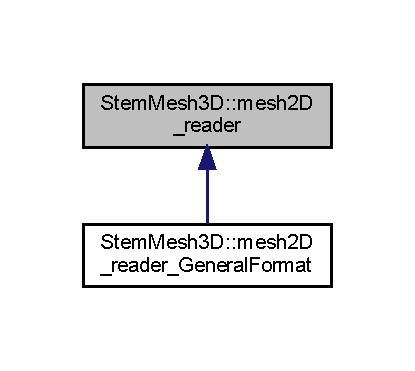
\includegraphics[width=199pt]{classStemMesh3D_1_1mesh2D__reader__inherit__graph}
\end{center}
\end{figure}
\subsection*{Public Member Functions}
\begin{DoxyCompactItemize}
\item 
\mbox{\Hypertarget{classStemMesh3D_1_1mesh2D__reader_add60d0182da92d539e7181f661339d04}\label{classStemMesh3D_1_1mesh2D__reader_add60d0182da92d539e7181f661339d04}} 
virtual void {\bfseries read\+\_\+mesh} (std\+::vector$<$ double $>$ \&xV, std\+::vector$<$ double $>$ \&yV, std\+::vector$<$ \hyperlink{classStemMesh3D_1_1mesh__3Dv_a9544cba555b60f17f04fcd1689314338}{mesh\+\_\+3\+Dv\+::flag\+\_\+type} $>$ \&fV, std\+::vector$<$ size\+\_\+t $>$ \&regn\+\_\+vlist, std\+::vector$<$ \hyperlink{classStemMesh3D_1_1mesh__3Dv_a9544cba555b60f17f04fcd1689314338}{mesh\+\_\+3\+Dv\+::flag\+\_\+type} $>$ \&fR)=0
\end{DoxyCompactItemize}
\subsection*{Protected Member Functions}
\begin{DoxyCompactItemize}
\item 
\mbox{\Hypertarget{classStemMesh3D_1_1mesh2D__reader_a178adde6c4b6e4e8d71de5b4891219cc}\label{classStemMesh3D_1_1mesh2D__reader_a178adde6c4b6e4e8d71de5b4891219cc}} 
void {\bfseries error\+\_\+message} (const std\+::string \&s)
\item 
\mbox{\Hypertarget{classStemMesh3D_1_1mesh2D__reader_acaaa656a532855ab4ef7b4a1887ca151}\label{classStemMesh3D_1_1mesh2D__reader_acaaa656a532855ab4ef7b4a1887ca151}} 
virtual void {\bfseries read\+\_\+vrtx\+\_\+data} (std\+::ifstream \&input\+\_\+file, std\+::vector$<$ double $>$ \&xV, std\+::vector$<$ double $>$ \&yV, std\+::vector$<$ \hyperlink{classStemMesh3D_1_1mesh__3Dv_a9544cba555b60f17f04fcd1689314338}{mesh\+\_\+3\+Dv\+::flag\+\_\+type} $>$ \&fV)=0
\item 
\mbox{\Hypertarget{classStemMesh3D_1_1mesh2D__reader_aa817255612a6468a4843a26b27561d0f}\label{classStemMesh3D_1_1mesh2D__reader_aa817255612a6468a4843a26b27561d0f}} 
virtual void {\bfseries read\+\_\+regn\+\_\+data} (std\+::ifstream \&input\+\_\+file, std\+::vector$<$ size\+\_\+t $>$ \&regn\+\_\+vlist, std\+::vector$<$ \hyperlink{classStemMesh3D_1_1mesh__3Dv_a9544cba555b60f17f04fcd1689314338}{mesh\+\_\+3\+Dv\+::flag\+\_\+type} $>$ \&fR)=0
\end{DoxyCompactItemize}
\subsection*{Static Protected Member Functions}
\begin{DoxyCompactItemize}
\item 
\mbox{\Hypertarget{classStemMesh3D_1_1mesh2D__reader_aedd5f683a45a7c28037b4cccae74211c}\label{classStemMesh3D_1_1mesh2D__reader_aedd5f683a45a7c28037b4cccae74211c}} 
static std\+::istream \& {\bfseries eatline} (std\+::istream \&s)
\item 
\mbox{\Hypertarget{classStemMesh3D_1_1mesh2D__reader_a8b241ba77a1527e82990b9729f2edb8b}\label{classStemMesh3D_1_1mesh2D__reader_a8b241ba77a1527e82990b9729f2edb8b}} 
static std\+::istream \& {\bfseries eatchar} (std\+::istream \&s)
\item 
\mbox{\Hypertarget{classStemMesh3D_1_1mesh2D__reader_aa546960ba60fa6b70f577ce5a879b752}\label{classStemMesh3D_1_1mesh2D__reader_aa546960ba60fa6b70f577ce5a879b752}} 
static std\+::istream \& {\bfseries eatcomments} (std\+::istream \&s)
\end{DoxyCompactItemize}


The documentation for this class was generated from the following file\+:\begin{DoxyCompactItemize}
\item 
src/\+Mesh/\+Stem\+Mesh/mesh3\+D\+\_\+format\+\_\+readers.\+hh\end{DoxyCompactItemize}

\hypertarget{classStemMesh3D_1_1mesh2D__reader__GeneralFormat}{}\section{Stem\+Mesh3D\+:\+:mesh2\+D\+\_\+reader\+\_\+\+General\+Format Class Reference}
\label{classStemMesh3D_1_1mesh2D__reader__GeneralFormat}\index{Stem\+Mesh3\+D\+::mesh2\+D\+\_\+reader\+\_\+\+General\+Format@{Stem\+Mesh3\+D\+::mesh2\+D\+\_\+reader\+\_\+\+General\+Format}}


Inheritance diagram for Stem\+Mesh3D\+:\+:mesh2\+D\+\_\+reader\+\_\+\+General\+Format\+:\nopagebreak
\begin{figure}[H]
\begin{center}
\leavevmode
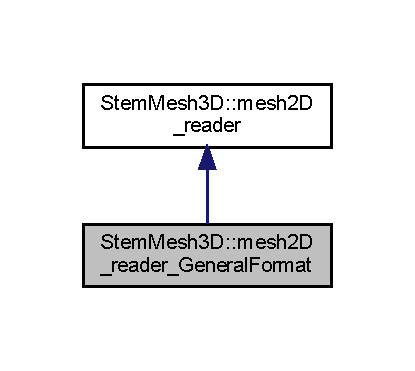
\includegraphics[width=199pt]{classStemMesh3D_1_1mesh2D__reader__GeneralFormat__inherit__graph}
\end{center}
\end{figure}


Collaboration diagram for Stem\+Mesh3D\+:\+:mesh2\+D\+\_\+reader\+\_\+\+General\+Format\+:\nopagebreak
\begin{figure}[H]
\begin{center}
\leavevmode
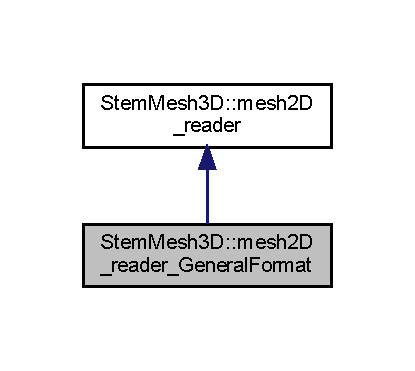
\includegraphics[width=199pt]{classStemMesh3D_1_1mesh2D__reader__GeneralFormat__coll__graph}
\end{center}
\end{figure}
\subsection*{Public Member Functions}
\begin{DoxyCompactItemize}
\item 
\mbox{\Hypertarget{classStemMesh3D_1_1mesh2D__reader__GeneralFormat_a773b0b9beba365bfc540c4050154bf2e}\label{classStemMesh3D_1_1mesh2D__reader__GeneralFormat_a773b0b9beba365bfc540c4050154bf2e}} 
{\bfseries mesh2\+D\+\_\+reader\+\_\+\+General\+Format} (std\+::string \+\_\+file\+\_\+name, size\+\_\+t \+\_\+offset=1)
\item 
\mbox{\Hypertarget{classStemMesh3D_1_1mesh2D__reader__GeneralFormat_a37ab61a2a4e9aababdee54e91aca81be}\label{classStemMesh3D_1_1mesh2D__reader__GeneralFormat_a37ab61a2a4e9aababdee54e91aca81be}} 
virtual void {\bfseries read\+\_\+mesh} (std\+::vector$<$ double $>$ \&xV, std\+::vector$<$ double $>$ \&yV, std\+::vector$<$ \hyperlink{classStemMesh3D_1_1mesh__3Dv_a9544cba555b60f17f04fcd1689314338}{mesh\+\_\+3\+Dv\+::flag\+\_\+type} $>$ \&fV, std\+::vector$<$ size\+\_\+t $>$ \&regn\+\_\+vlist, std\+::vector$<$ \hyperlink{classStemMesh3D_1_1mesh__3Dv_a9544cba555b60f17f04fcd1689314338}{mesh\+\_\+3\+Dv\+::flag\+\_\+type} $>$ \&fR)
\end{DoxyCompactItemize}
\subsection*{Protected Member Functions}
\begin{DoxyCompactItemize}
\item 
\mbox{\Hypertarget{classStemMesh3D_1_1mesh2D__reader__GeneralFormat_a4a4ae19f3aa529054c00d345171e9146}\label{classStemMesh3D_1_1mesh2D__reader__GeneralFormat_a4a4ae19f3aa529054c00d345171e9146}} 
virtual void {\bfseries read\+\_\+vrtx\+\_\+data} (std\+::ifstream \&input\+\_\+file, std\+::vector$<$ double $>$ \&xV, std\+::vector$<$ double $>$ \&yV, std\+::vector$<$ \hyperlink{classStemMesh3D_1_1mesh__3Dv_a9544cba555b60f17f04fcd1689314338}{mesh\+\_\+3\+Dv\+::flag\+\_\+type} $>$ \&fV)
\item 
\mbox{\Hypertarget{classStemMesh3D_1_1mesh2D__reader__GeneralFormat_a3fdc49ff130caa2aa233f4364dcf44a0}\label{classStemMesh3D_1_1mesh2D__reader__GeneralFormat_a3fdc49ff130caa2aa233f4364dcf44a0}} 
virtual void {\bfseries read\+\_\+regn\+\_\+data} (std\+::ifstream \&input\+\_\+file, std\+::vector$<$ size\+\_\+t $>$ \&regn\+\_\+vlist, std\+::vector$<$ \hyperlink{classStemMesh3D_1_1mesh__3Dv_a9544cba555b60f17f04fcd1689314338}{mesh\+\_\+3\+Dv\+::flag\+\_\+type} $>$ \&fR)
\end{DoxyCompactItemize}
\subsection*{Additional Inherited Members}


The documentation for this class was generated from the following file\+:\begin{DoxyCompactItemize}
\item 
src/\+Mesh/\+Stem\+Mesh/mesh3\+D\+\_\+format\+\_\+readers.\+hh\end{DoxyCompactItemize}

\hypertarget{classStemMesh3D_1_1mesh3D__reader}{}\doxysection{Stem\+Mesh3D\+::mesh3\+D\+\_\+reader Class Reference}
\label{classStemMesh3D_1_1mesh3D__reader}\index{StemMesh3D::mesh3D\_reader@{StemMesh3D::mesh3D\_reader}}


Inheritance diagram for Stem\+Mesh3D\+::mesh3\+D\+\_\+reader\+:\nopagebreak
\begin{figure}[H]
\begin{center}
\leavevmode
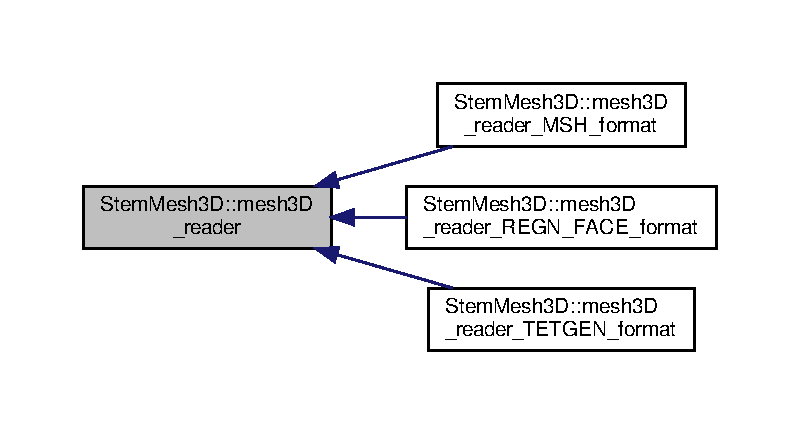
\includegraphics[width=350pt]{classStemMesh3D_1_1mesh3D__reader__inherit__graph}
\end{center}
\end{figure}
\doxysubsection*{Public Member Functions}
\begin{DoxyCompactItemize}
\item 
\mbox{\Hypertarget{classStemMesh3D_1_1mesh3D__reader_adc698cd5b3b732eaba1772a3c99892bd}\label{classStemMesh3D_1_1mesh3D__reader_adc698cd5b3b732eaba1772a3c99892bd}} 
virtual void {\bfseries read\+\_\+the\+\_\+mesh} (std\+::vector$<$ double $>$ \&xV, std\+::vector$<$ double $>$ \&yV, std\+::vector$<$ double $>$ \&zV, std\+::vector$<$ \mbox{\hyperlink{classStemMesh3D_1_1mesh__3Dv_a9544cba555b60f17f04fcd1689314338}{mesh\+\_\+3\+Dv\+::flag\+\_\+type}} $>$ \&fV, std\+::vector$<$ size\+\_\+t $>$ \&regn\+\_\+vlist, std\+::vector$<$ \mbox{\hyperlink{classStemMesh3D_1_1mesh__3Dv_a9544cba555b60f17f04fcd1689314338}{mesh\+\_\+3\+Dv\+::flag\+\_\+type}} $>$ \&fR)=0
\end{DoxyCompactItemize}
\doxysubsection*{Protected Member Functions}
\begin{DoxyCompactItemize}
\item 
\mbox{\Hypertarget{classStemMesh3D_1_1mesh3D__reader_a67dd32389104f45a0e846318f131d371}\label{classStemMesh3D_1_1mesh3D__reader_a67dd32389104f45a0e846318f131d371}} 
void {\bfseries error\+\_\+message} (const std\+::string \&s)
\item 
\mbox{\Hypertarget{classStemMesh3D_1_1mesh3D__reader_a49552bdac73d0e0156e0bac1b9b914b9}\label{classStemMesh3D_1_1mesh3D__reader_a49552bdac73d0e0156e0bac1b9b914b9}} 
virtual void {\bfseries read\+\_\+vrtx\+\_\+data} (std\+::ifstream \&input\+\_\+file, std\+::vector$<$ double $>$ \&xV, std\+::vector$<$ double $>$ \&yV, std\+::vector$<$ double $>$ \&zV, std\+::vector$<$ \mbox{\hyperlink{classStemMesh3D_1_1mesh__3Dv_a9544cba555b60f17f04fcd1689314338}{mesh\+\_\+3\+Dv\+::flag\+\_\+type}} $>$ \&fV)=0
\item 
\mbox{\Hypertarget{classStemMesh3D_1_1mesh3D__reader_a108c6a647a67014a09120cb46a971d5d}\label{classStemMesh3D_1_1mesh3D__reader_a108c6a647a67014a09120cb46a971d5d}} 
virtual void {\bfseries read\+\_\+regn\+\_\+data} (std\+::ifstream \&input\+\_\+file, std\+::vector$<$ size\+\_\+t $>$ \&regn\+\_\+vlist, std\+::vector$<$ \mbox{\hyperlink{classStemMesh3D_1_1mesh__3Dv_a9544cba555b60f17f04fcd1689314338}{mesh\+\_\+3\+Dv\+::flag\+\_\+type}} $>$ \&fR)=0
\end{DoxyCompactItemize}
\doxysubsection*{Static Protected Member Functions}
\begin{DoxyCompactItemize}
\item 
\mbox{\Hypertarget{classStemMesh3D_1_1mesh3D__reader_ab094d54022615427f5f5cf4ea04b2cb9}\label{classStemMesh3D_1_1mesh3D__reader_ab094d54022615427f5f5cf4ea04b2cb9}} 
static std\+::istream \& {\bfseries eatline} (std\+::istream \&s)
\item 
\mbox{\Hypertarget{classStemMesh3D_1_1mesh3D__reader_aa14b098edf06fedc72676af589ca8684}\label{classStemMesh3D_1_1mesh3D__reader_aa14b098edf06fedc72676af589ca8684}} 
static std\+::istream \& {\bfseries eatchar} (std\+::istream \&s)
\item 
\mbox{\Hypertarget{classStemMesh3D_1_1mesh3D__reader_ab09cc7c2ed6ffa191f45e87f136168e0}\label{classStemMesh3D_1_1mesh3D__reader_ab09cc7c2ed6ffa191f45e87f136168e0}} 
static std\+::istream \& {\bfseries eatcomments} (std\+::istream \&s)
\end{DoxyCompactItemize}


The documentation for this class was generated from the following file\+:\begin{DoxyCompactItemize}
\item 
src/\+Mesh/\+Stem\+Mesh/mesh3\+D\+\_\+format\+\_\+readers.\+hh\end{DoxyCompactItemize}

\hypertarget{classStemMesh3D_1_1mesh3D__reader__MSH__format}{}\section{Stem\+Mesh3D\+:\+:mesh3\+D\+\_\+reader\+\_\+\+M\+S\+H\+\_\+format Class Reference}
\label{classStemMesh3D_1_1mesh3D__reader__MSH__format}\index{Stem\+Mesh3\+D\+::mesh3\+D\+\_\+reader\+\_\+\+M\+S\+H\+\_\+format@{Stem\+Mesh3\+D\+::mesh3\+D\+\_\+reader\+\_\+\+M\+S\+H\+\_\+format}}


Inheritance diagram for Stem\+Mesh3D\+:\+:mesh3\+D\+\_\+reader\+\_\+\+M\+S\+H\+\_\+format\+:\nopagebreak
\begin{figure}[H]
\begin{center}
\leavevmode
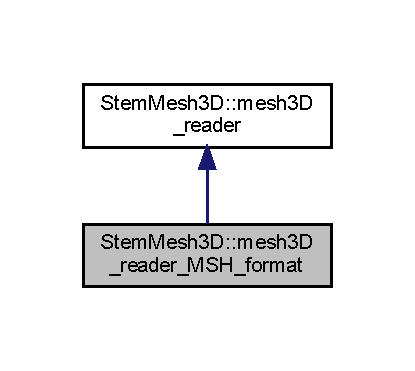
\includegraphics[width=199pt]{classStemMesh3D_1_1mesh3D__reader__MSH__format__inherit__graph}
\end{center}
\end{figure}


Collaboration diagram for Stem\+Mesh3D\+:\+:mesh3\+D\+\_\+reader\+\_\+\+M\+S\+H\+\_\+format\+:\nopagebreak
\begin{figure}[H]
\begin{center}
\leavevmode
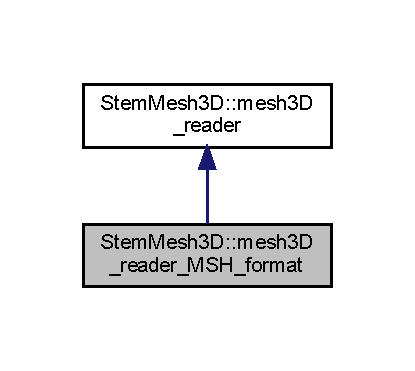
\includegraphics[width=199pt]{classStemMesh3D_1_1mesh3D__reader__MSH__format__coll__graph}
\end{center}
\end{figure}
\subsection*{Public Member Functions}
\begin{DoxyCompactItemize}
\item 
\mbox{\Hypertarget{classStemMesh3D_1_1mesh3D__reader__MSH__format_a67c1165302d6a97406675d39993666f6}\label{classStemMesh3D_1_1mesh3D__reader__MSH__format_a67c1165302d6a97406675d39993666f6}} 
{\bfseries mesh3\+D\+\_\+reader\+\_\+\+M\+S\+H\+\_\+format} (std\+::string \+\_\+file\+\_\+name, size\+\_\+t \+\_\+offset=1)
\item 
\mbox{\Hypertarget{classStemMesh3D_1_1mesh3D__reader__MSH__format_a8b169633cf81623a612493c54a0c7457}\label{classStemMesh3D_1_1mesh3D__reader__MSH__format_a8b169633cf81623a612493c54a0c7457}} 
virtual void {\bfseries read\+\_\+the\+\_\+mesh} (std\+::vector$<$ double $>$ \&xV, std\+::vector$<$ double $>$ \&yV, std\+::vector$<$ double $>$ \&zV, std\+::vector$<$ \hyperlink{classStemMesh3D_1_1mesh__3Dv_a9544cba555b60f17f04fcd1689314338}{mesh\+\_\+3\+Dv\+::flag\+\_\+type} $>$ \&fV, std\+::vector$<$ size\+\_\+t $>$ \&regn\+\_\+vlist, std\+::vector$<$ \hyperlink{classStemMesh3D_1_1mesh__3Dv_a9544cba555b60f17f04fcd1689314338}{mesh\+\_\+3\+Dv\+::flag\+\_\+type} $>$ \&fR)
\item 
\mbox{\Hypertarget{classStemMesh3D_1_1mesh3D__reader__MSH__format_af5e4903620880fa64f9d42da9a419e53}\label{classStemMesh3D_1_1mesh3D__reader__MSH__format_af5e4903620880fa64f9d42da9a419e53}} 
{\footnotesize template$<$typename T $>$ }\\void {\bfseries print\+\_\+vector} (std\+::vector$<$ std\+::vector$<$ T $>$ $>$ \&vec, size\+\_\+t nvec)
\end{DoxyCompactItemize}
\subsection*{Protected Member Functions}
\begin{DoxyCompactItemize}
\item 
\mbox{\Hypertarget{classStemMesh3D_1_1mesh3D__reader__MSH__format_a9bdd28a087cd1f0d91b403d5464b7545}\label{classStemMesh3D_1_1mesh3D__reader__MSH__format_a9bdd28a087cd1f0d91b403d5464b7545}} 
virtual void {\bfseries read\+\_\+vrtx\+\_\+data} (std\+::ifstream \&input\+\_\+file, std\+::vector$<$ double $>$ \&xV, std\+::vector$<$ double $>$ \&yV, std\+::vector$<$ double $>$ \&zV, std\+::vector$<$ \hyperlink{classStemMesh3D_1_1mesh__3Dv_a9544cba555b60f17f04fcd1689314338}{mesh\+\_\+3\+Dv\+::flag\+\_\+type} $>$ \&fV)
\item 
\mbox{\Hypertarget{classStemMesh3D_1_1mesh3D__reader__MSH__format_a9439cde7f173dba6130178047ccdc3ce}\label{classStemMesh3D_1_1mesh3D__reader__MSH__format_a9439cde7f173dba6130178047ccdc3ce}} 
virtual void {\bfseries read\+\_\+regn\+\_\+data} (std\+::ifstream \&input\+\_\+file, std\+::vector$<$ size\+\_\+t $>$ \&regn\+\_\+vlist, std\+::vector$<$ \hyperlink{classStemMesh3D_1_1mesh__3Dv_a9544cba555b60f17f04fcd1689314338}{mesh\+\_\+3\+Dv\+::flag\+\_\+type} $>$ \&fR)
\end{DoxyCompactItemize}
\subsection*{Additional Inherited Members}


The documentation for this class was generated from the following file\+:\begin{DoxyCompactItemize}
\item 
src/\+Mesh/\+Stem\+Mesh/mesh3\+D\+\_\+format\+\_\+readers.\+hh\end{DoxyCompactItemize}

\hypertarget{classStemMesh3D_1_1mesh3D__reader__REGN__FACE__format}{}\doxysection{Stem\+Mesh3D\+::mesh3\+D\+\_\+reader\+\_\+\+R\+E\+G\+N\+\_\+\+F\+A\+C\+E\+\_\+format Class Reference}
\label{classStemMesh3D_1_1mesh3D__reader__REGN__FACE__format}\index{StemMesh3D::mesh3D\_reader\_REGN\_FACE\_format@{StemMesh3D::mesh3D\_reader\_REGN\_FACE\_format}}


Inheritance diagram for Stem\+Mesh3D\+::mesh3\+D\+\_\+reader\+\_\+\+R\+E\+G\+N\+\_\+\+F\+A\+C\+E\+\_\+format\+:\nopagebreak
\begin{figure}[H]
\begin{center}
\leavevmode
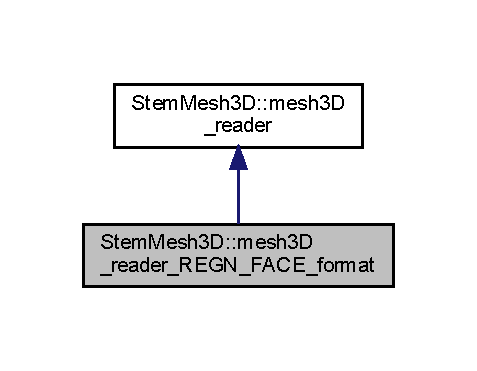
\includegraphics[width=229pt]{classStemMesh3D_1_1mesh3D__reader__REGN__FACE__format__inherit__graph}
\end{center}
\end{figure}


Collaboration diagram for Stem\+Mesh3D\+::mesh3\+D\+\_\+reader\+\_\+\+R\+E\+G\+N\+\_\+\+F\+A\+C\+E\+\_\+format\+:\nopagebreak
\begin{figure}[H]
\begin{center}
\leavevmode
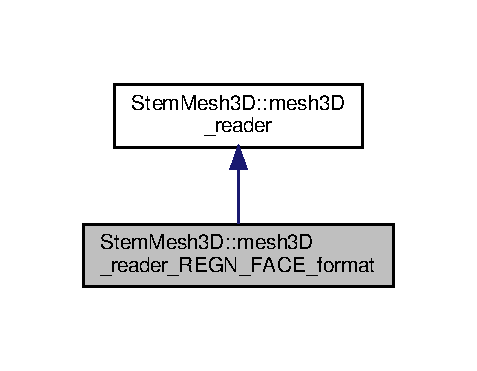
\includegraphics[width=229pt]{classStemMesh3D_1_1mesh3D__reader__REGN__FACE__format__coll__graph}
\end{center}
\end{figure}
\doxysubsection*{Public Member Functions}
\begin{DoxyCompactItemize}
\item 
\mbox{\Hypertarget{classStemMesh3D_1_1mesh3D__reader__REGN__FACE__format_aaa9eda98a389418706b7e1a81dce813f}\label{classStemMesh3D_1_1mesh3D__reader__REGN__FACE__format_aaa9eda98a389418706b7e1a81dce813f}} 
{\bfseries mesh3\+D\+\_\+reader\+\_\+\+R\+E\+G\+N\+\_\+\+F\+A\+C\+E\+\_\+format} (std\+::string \+\_\+file\+\_\+name, size\+\_\+t \+\_\+offset=1)
\item 
\mbox{\Hypertarget{classStemMesh3D_1_1mesh3D__reader__REGN__FACE__format_ae26b342564034d6e76965c8cf34cdbd1}\label{classStemMesh3D_1_1mesh3D__reader__REGN__FACE__format_ae26b342564034d6e76965c8cf34cdbd1}} 
virtual void {\bfseries read\+\_\+the\+\_\+mesh} (std\+::vector$<$ double $>$ \&xV, std\+::vector$<$ double $>$ \&yV, std\+::vector$<$ double $>$ \&zV, std\+::vector$<$ \mbox{\hyperlink{classStemMesh3D_1_1mesh__3Dv_a9544cba555b60f17f04fcd1689314338}{mesh\+\_\+3\+Dv\+::flag\+\_\+type}} $>$ \&fV, std\+::vector$<$ size\+\_\+t $>$ \&regn\+\_\+flist, std\+::vector$<$ \mbox{\hyperlink{classStemMesh3D_1_1mesh__3Dv_a9544cba555b60f17f04fcd1689314338}{mesh\+\_\+3\+Dv\+::flag\+\_\+type}} $>$ \&fR)
\end{DoxyCompactItemize}
\doxysubsection*{Protected Member Functions}
\begin{DoxyCompactItemize}
\item 
\mbox{\Hypertarget{classStemMesh3D_1_1mesh3D__reader__REGN__FACE__format_aee9bd0898e4e2dc06c70019e289ca60c}\label{classStemMesh3D_1_1mesh3D__reader__REGN__FACE__format_aee9bd0898e4e2dc06c70019e289ca60c}} 
virtual void {\bfseries read\+\_\+vrtx\+\_\+data} (std\+::ifstream \&input\+\_\+file, std\+::vector$<$ double $>$ \&xV, std\+::vector$<$ double $>$ \&yV, std\+::vector$<$ double $>$ \&zV, std\+::vector$<$ \mbox{\hyperlink{classStemMesh3D_1_1mesh__3Dv_a9544cba555b60f17f04fcd1689314338}{mesh\+\_\+3\+Dv\+::flag\+\_\+type}} $>$ \&fV)
\item 
\mbox{\Hypertarget{classStemMesh3D_1_1mesh3D__reader__REGN__FACE__format_a5c7cc5b38794e5f2ee56dbf1bdf3ab76}\label{classStemMesh3D_1_1mesh3D__reader__REGN__FACE__format_a5c7cc5b38794e5f2ee56dbf1bdf3ab76}} 
virtual void {\bfseries read\+\_\+regn\+\_\+data} (std\+::ifstream \&input\+\_\+file, std\+::vector$<$ size\+\_\+t $>$ \&regn\+\_\+flist, std\+::vector$<$ \mbox{\hyperlink{classStemMesh3D_1_1mesh__3Dv_a9544cba555b60f17f04fcd1689314338}{mesh\+\_\+3\+Dv\+::flag\+\_\+type}} $>$ \&fR)
\end{DoxyCompactItemize}
\doxysubsection*{Additional Inherited Members}


The documentation for this class was generated from the following file\+:\begin{DoxyCompactItemize}
\item 
src/\+Mesh/\+Stem\+Mesh/mesh3\+D\+\_\+format\+\_\+readers.\+hh\end{DoxyCompactItemize}

\hypertarget{classStemMesh3D_1_1mesh3D__reader__TETGEN__format}{}\section{Stem\+Mesh3D\+:\+:mesh3\+D\+\_\+reader\+\_\+\+T\+E\+T\+G\+E\+N\+\_\+format Class Reference}
\label{classStemMesh3D_1_1mesh3D__reader__TETGEN__format}\index{Stem\+Mesh3\+D\+::mesh3\+D\+\_\+reader\+\_\+\+T\+E\+T\+G\+E\+N\+\_\+format@{Stem\+Mesh3\+D\+::mesh3\+D\+\_\+reader\+\_\+\+T\+E\+T\+G\+E\+N\+\_\+format}}


Inheritance diagram for Stem\+Mesh3D\+:\+:mesh3\+D\+\_\+reader\+\_\+\+T\+E\+T\+G\+E\+N\+\_\+format\+:\nopagebreak
\begin{figure}[H]
\begin{center}
\leavevmode
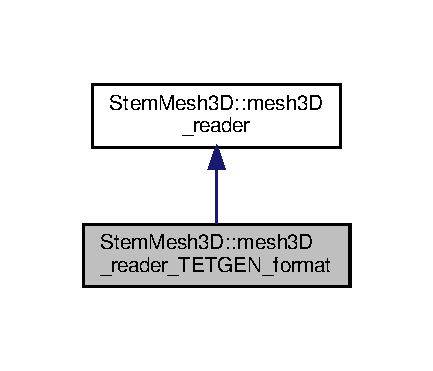
\includegraphics[width=208pt]{classStemMesh3D_1_1mesh3D__reader__TETGEN__format__inherit__graph}
\end{center}
\end{figure}


Collaboration diagram for Stem\+Mesh3D\+:\+:mesh3\+D\+\_\+reader\+\_\+\+T\+E\+T\+G\+E\+N\+\_\+format\+:\nopagebreak
\begin{figure}[H]
\begin{center}
\leavevmode
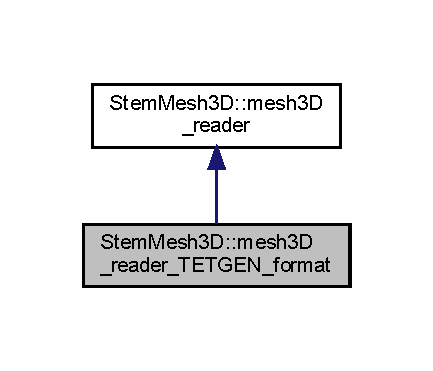
\includegraphics[width=208pt]{classStemMesh3D_1_1mesh3D__reader__TETGEN__format__coll__graph}
\end{center}
\end{figure}
\subsection*{Public Member Functions}
\begin{DoxyCompactItemize}
\item 
\mbox{\Hypertarget{classStemMesh3D_1_1mesh3D__reader__TETGEN__format_a73608ffd33247cdc03cbfd2c507e44c1}\label{classStemMesh3D_1_1mesh3D__reader__TETGEN__format_a73608ffd33247cdc03cbfd2c507e44c1}} 
{\bfseries mesh3\+D\+\_\+reader\+\_\+\+T\+E\+T\+G\+E\+N\+\_\+format} (std\+::string \+\_\+file\+\_\+name, size\+\_\+t \+\_\+offset=1)
\item 
\mbox{\Hypertarget{classStemMesh3D_1_1mesh3D__reader__TETGEN__format_a07a29d1335c5c8f4adb1af49be254fde}\label{classStemMesh3D_1_1mesh3D__reader__TETGEN__format_a07a29d1335c5c8f4adb1af49be254fde}} 
virtual void {\bfseries read\+\_\+the\+\_\+mesh} (std\+::vector$<$ double $>$ \&xV, std\+::vector$<$ double $>$ \&yV, std\+::vector$<$ double $>$ \&zV, std\+::vector$<$ \hyperlink{classStemMesh3D_1_1mesh__3Dv_a9544cba555b60f17f04fcd1689314338}{mesh\+\_\+3\+Dv\+::flag\+\_\+type} $>$ \&fV, std\+::vector$<$ size\+\_\+t $>$ \&regn\+\_\+vlist, std\+::vector$<$ \hyperlink{classStemMesh3D_1_1mesh__3Dv_a9544cba555b60f17f04fcd1689314338}{mesh\+\_\+3\+Dv\+::flag\+\_\+type} $>$ \&fR)
\end{DoxyCompactItemize}
\subsection*{Protected Member Functions}
\begin{DoxyCompactItemize}
\item 
\mbox{\Hypertarget{classStemMesh3D_1_1mesh3D__reader__TETGEN__format_a60a1ec3c1931d8945b217f26c0f49053}\label{classStemMesh3D_1_1mesh3D__reader__TETGEN__format_a60a1ec3c1931d8945b217f26c0f49053}} 
virtual void {\bfseries read\+\_\+vrtx\+\_\+data} (std\+::ifstream \&input\+\_\+file, std\+::vector$<$ double $>$ \&xV, std\+::vector$<$ double $>$ \&yV, std\+::vector$<$ double $>$ \&zV, std\+::vector$<$ \hyperlink{classStemMesh3D_1_1mesh__3Dv_a9544cba555b60f17f04fcd1689314338}{mesh\+\_\+3\+Dv\+::flag\+\_\+type} $>$ \&fV)
\item 
\mbox{\Hypertarget{classStemMesh3D_1_1mesh3D__reader__TETGEN__format_a9ce35774f3e82a7fb367d66ab38132f3}\label{classStemMesh3D_1_1mesh3D__reader__TETGEN__format_a9ce35774f3e82a7fb367d66ab38132f3}} 
virtual void {\bfseries read\+\_\+regn\+\_\+data} (std\+::ifstream \&input\+\_\+file, std\+::vector$<$ size\+\_\+t $>$ \&regn\+\_\+vlist, std\+::vector$<$ \hyperlink{classStemMesh3D_1_1mesh__3Dv_a9544cba555b60f17f04fcd1689314338}{mesh\+\_\+3\+Dv\+::flag\+\_\+type} $>$ \&fR)
\end{DoxyCompactItemize}
\subsection*{Additional Inherited Members}


The documentation for this class was generated from the following file\+:\begin{DoxyCompactItemize}
\item 
src/\+Mesh/\+Stem\+Mesh/mesh3\+D\+\_\+format\+\_\+readers.\+hh\end{DoxyCompactItemize}

\hypertarget{classStemMesh3D_1_1mesh3Dv__builder}{}\section{Stem\+Mesh3D\+:\+:mesh3\+Dv\+\_\+builder Class Reference}
\label{classStemMesh3D_1_1mesh3Dv__builder}\index{Stem\+Mesh3\+D\+::mesh3\+Dv\+\_\+builder@{Stem\+Mesh3\+D\+::mesh3\+Dv\+\_\+builder}}
\subsection*{Public Member Functions}
\begin{DoxyCompactItemize}
\item 
\mbox{\Hypertarget{classStemMesh3D_1_1mesh3Dv__builder_a9d137944a599ff6f41ef321838ae2f18}\label{classStemMesh3D_1_1mesh3Dv__builder_a9d137944a599ff6f41ef321838ae2f18}} 
{\bfseries mesh3\+Dv\+\_\+builder} (\hyperlink{classStemMesh3D_1_1mesh__3Dv}{mesh\+\_\+3\+Dv} \&\+\_\+mesh)
\item 
\mbox{\Hypertarget{classStemMesh3D_1_1mesh3Dv__builder_a05588bb9dff04c8a96e5785edf8932d2}\label{classStemMesh3D_1_1mesh3Dv__builder_a05588bb9dff04c8a96e5785edf8932d2}} 
void {\bfseries change\+\_\+bbox} (double new\+\_\+xmin, double new\+\_\+ymin, double new\+\_\+zmin, double new\+\_\+xmax, double new\+\_\+ymax, double new\+\_\+zmax)
\item 
\mbox{\Hypertarget{classStemMesh3D_1_1mesh3Dv__builder_a558c4675f98eec141945e26e709b1753}\label{classStemMesh3D_1_1mesh3Dv__builder_a558c4675f98eec141945e26e709b1753}} 
void {\bfseries build\+\_\+the\+\_\+mesh} (std\+::vector$<$ double $>$ \&xV, std\+::vector$<$ double $>$ \&yV, std\+::vector$<$ double $>$ \&zV, std\+::vector$<$ \hyperlink{classStemMesh3D_1_1mesh__3Dv_a9544cba555b60f17f04fcd1689314338}{mesh\+\_\+3\+Dv\+::flag\+\_\+type} $>$ \&fV, std\+::vector$<$ size\+\_\+t $>$ \&regn\+\_\+flist, std\+::vector$<$ \hyperlink{classStemMesh3D_1_1mesh__3Dv_a9544cba555b60f17f04fcd1689314338}{mesh\+\_\+3\+Dv\+::flag\+\_\+type} $>$ \&fR)
\end{DoxyCompactItemize}


The documentation for this class was generated from the following file\+:\begin{DoxyCompactItemize}
\item 
src/\+Mesh/\+Stem\+Mesh/builder.\+hh\end{DoxyCompactItemize}

\hypertarget{classStemMesh3D_1_1mesh3Dv__cmaster}{}\section{Stem\+Mesh3D\+:\+:mesh3\+Dv\+\_\+cmaster Class Reference}
\label{classStemMesh3D_1_1mesh3Dv__cmaster}\index{Stem\+Mesh3\+D\+::mesh3\+Dv\+\_\+cmaster@{Stem\+Mesh3\+D\+::mesh3\+Dv\+\_\+cmaster}}
\subsection*{Public Member Functions}
\begin{DoxyCompactItemize}
\item 
\mbox{\Hypertarget{classStemMesh3D_1_1mesh3Dv__cmaster_a5f173d546a048c0b8e5ab97dedcae2f3}\label{classStemMesh3D_1_1mesh3Dv__cmaster_a5f173d546a048c0b8e5ab97dedcae2f3}} 
{\bfseries mesh3\+Dv\+\_\+cmaster} (\hyperlink{classStemMesh3D_1_1mesh__3Dv}{mesh\+\_\+3\+Dv} \&\+\_\+mesh)
\item 
\mbox{\Hypertarget{classStemMesh3D_1_1mesh3Dv__cmaster_adebe008c2a1a5cb80796598a607e3a17}\label{classStemMesh3D_1_1mesh3Dv__cmaster_adebe008c2a1a5cb80796598a607e3a17}} 
void {\bfseries check\+\_\+the\+\_\+mesh} ()
\item 
\mbox{\Hypertarget{classStemMesh3D_1_1mesh3Dv__cmaster_a152f66d7e9d03b559bcd6a7f8814e8f9}\label{classStemMesh3D_1_1mesh3Dv__cmaster_a152f66d7e9d03b559bcd6a7f8814e8f9}} 
bool {\bfseries check\+\_\+the\+\_\+regions} ()
\item 
\mbox{\Hypertarget{classStemMesh3D_1_1mesh3Dv__cmaster_a61a6d5816db89690e551bcb182662ece}\label{classStemMesh3D_1_1mesh3Dv__cmaster_a61a6d5816db89690e551bcb182662ece}} 
bool {\bfseries check\+\_\+regn\+\_\+regn} (size\+\_\+t i)
\item 
\mbox{\Hypertarget{classStemMesh3D_1_1mesh3Dv__cmaster_a1b0d14413e110f44c1949448a525ba99}\label{classStemMesh3D_1_1mesh3Dv__cmaster_a1b0d14413e110f44c1949448a525ba99}} 
bool {\bfseries check\+\_\+regn\+\_\+face} (size\+\_\+t i)
\item 
\mbox{\Hypertarget{classStemMesh3D_1_1mesh3Dv__cmaster_a0f64ae92708cac17ce2182191be54df9}\label{classStemMesh3D_1_1mesh3Dv__cmaster_a0f64ae92708cac17ce2182191be54df9}} 
bool {\bfseries check\+\_\+regn\+\_\+edge} (size\+\_\+t i)
\item 
\mbox{\Hypertarget{classStemMesh3D_1_1mesh3Dv__cmaster_a17ae764e6d0ecc435226f4ad5faa6334}\label{classStemMesh3D_1_1mesh3Dv__cmaster_a17ae764e6d0ecc435226f4ad5faa6334}} 
bool {\bfseries check\+\_\+regn\+\_\+vrtx} (size\+\_\+t i)
\item 
\mbox{\Hypertarget{classStemMesh3D_1_1mesh3Dv__cmaster_a7f578ff3d99f336eb5698c7fd9d6930e}\label{classStemMesh3D_1_1mesh3Dv__cmaster_a7f578ff3d99f336eb5698c7fd9d6930e}} 
bool {\bfseries check\+\_\+the\+\_\+faces} ()
\item 
\mbox{\Hypertarget{classStemMesh3D_1_1mesh3Dv__cmaster_acb031c380abc2e94caddd11d554d8794}\label{classStemMesh3D_1_1mesh3Dv__cmaster_acb031c380abc2e94caddd11d554d8794}} 
bool {\bfseries check\+\_\+face\+\_\+regn} (size\+\_\+t i)
\item 
\mbox{\Hypertarget{classStemMesh3D_1_1mesh3Dv__cmaster_a8880148e19a6151c38f192d4c2129c34}\label{classStemMesh3D_1_1mesh3Dv__cmaster_a8880148e19a6151c38f192d4c2129c34}} 
bool {\bfseries check\+\_\+face\+\_\+face} (size\+\_\+t i)
\item 
\mbox{\Hypertarget{classStemMesh3D_1_1mesh3Dv__cmaster_af80251d5f0542926533150cd48b8af40}\label{classStemMesh3D_1_1mesh3Dv__cmaster_af80251d5f0542926533150cd48b8af40}} 
bool {\bfseries check\+\_\+face\+\_\+edge} (size\+\_\+t i)
\item 
\mbox{\Hypertarget{classStemMesh3D_1_1mesh3Dv__cmaster_a4d2da6533fae24500176972964e989a9}\label{classStemMesh3D_1_1mesh3Dv__cmaster_a4d2da6533fae24500176972964e989a9}} 
bool {\bfseries check\+\_\+face\+\_\+vrtx} (size\+\_\+t i)
\item 
\mbox{\Hypertarget{classStemMesh3D_1_1mesh3Dv__cmaster_ad36d32aba1137f39334ef3c34870fb32}\label{classStemMesh3D_1_1mesh3Dv__cmaster_ad36d32aba1137f39334ef3c34870fb32}} 
bool {\bfseries check\+\_\+the\+\_\+edges} ()
\item 
\mbox{\Hypertarget{classStemMesh3D_1_1mesh3Dv__cmaster_a11b597bab996b539579b198adcf08b46}\label{classStemMesh3D_1_1mesh3Dv__cmaster_a11b597bab996b539579b198adcf08b46}} 
bool {\bfseries check\+\_\+edge\+\_\+regn} (size\+\_\+t i)
\item 
\mbox{\Hypertarget{classStemMesh3D_1_1mesh3Dv__cmaster_a431b8cef554f8878ed1d3cccdb19866c}\label{classStemMesh3D_1_1mesh3Dv__cmaster_a431b8cef554f8878ed1d3cccdb19866c}} 
bool {\bfseries check\+\_\+edge\+\_\+face} (size\+\_\+t i)
\item 
\mbox{\Hypertarget{classStemMesh3D_1_1mesh3Dv__cmaster_aabf356eae46a677cc0715578ae865bf5}\label{classStemMesh3D_1_1mesh3Dv__cmaster_aabf356eae46a677cc0715578ae865bf5}} 
bool {\bfseries check\+\_\+edge\+\_\+edge} (size\+\_\+t i)
\item 
\mbox{\Hypertarget{classStemMesh3D_1_1mesh3Dv__cmaster_a63b8aea2ac2a6836bc2c45236bc1c839}\label{classStemMesh3D_1_1mesh3Dv__cmaster_a63b8aea2ac2a6836bc2c45236bc1c839}} 
bool {\bfseries check\+\_\+edge\+\_\+vrtx} (size\+\_\+t i)
\item 
\mbox{\Hypertarget{classStemMesh3D_1_1mesh3Dv__cmaster_a0a7414c2f434a9d2e6d70d322bf03425}\label{classStemMesh3D_1_1mesh3Dv__cmaster_a0a7414c2f434a9d2e6d70d322bf03425}} 
bool {\bfseries check\+\_\+the\+\_\+vertices} ()
\item 
\mbox{\Hypertarget{classStemMesh3D_1_1mesh3Dv__cmaster_a3845c4e70b00a0814c9d8ac75b277862}\label{classStemMesh3D_1_1mesh3Dv__cmaster_a3845c4e70b00a0814c9d8ac75b277862}} 
bool {\bfseries check\+\_\+vrtx\+\_\+regn} (size\+\_\+t i)
\item 
\mbox{\Hypertarget{classStemMesh3D_1_1mesh3Dv__cmaster_a447647cb19d479004349a99b2625c227}\label{classStemMesh3D_1_1mesh3Dv__cmaster_a447647cb19d479004349a99b2625c227}} 
bool {\bfseries check\+\_\+vrtx\+\_\+face} (size\+\_\+t i)
\item 
\mbox{\Hypertarget{classStemMesh3D_1_1mesh3Dv__cmaster_a96dddec2393f5cb1f58f46de5d2b0a6d}\label{classStemMesh3D_1_1mesh3Dv__cmaster_a96dddec2393f5cb1f58f46de5d2b0a6d}} 
bool {\bfseries check\+\_\+vrtx\+\_\+edge} (size\+\_\+t i)
\item 
\mbox{\Hypertarget{classStemMesh3D_1_1mesh3Dv__cmaster_add9588de42c89223a82c472918a1d6fb}\label{classStemMesh3D_1_1mesh3Dv__cmaster_add9588de42c89223a82c472918a1d6fb}} 
bool {\bfseries check\+\_\+vrtx\+\_\+vrtx} (size\+\_\+t i)
\item 
\mbox{\Hypertarget{classStemMesh3D_1_1mesh3Dv__cmaster_a2e5c1fb4f1448d391094ef4289f42992}\label{classStemMesh3D_1_1mesh3Dv__cmaster_a2e5c1fb4f1448d391094ef4289f42992}} 
bool {\bfseries check\+\_\+local\+\_\+regions} ()
\item 
\mbox{\Hypertarget{classStemMesh3D_1_1mesh3Dv__cmaster_aafef56d92478adbac1e39b134206aa1e}\label{classStemMesh3D_1_1mesh3Dv__cmaster_aafef56d92478adbac1e39b134206aa1e}} 
bool {\bfseries check\+\_\+local\+\_\+faces} ()
\item 
\mbox{\Hypertarget{classStemMesh3D_1_1mesh3Dv__cmaster_a0e1e7560e37375a6d836e7fcb6c747a0}\label{classStemMesh3D_1_1mesh3Dv__cmaster_a0e1e7560e37375a6d836e7fcb6c747a0}} 
bool {\bfseries check\+\_\+local\+\_\+edges} ()
\item 
\mbox{\Hypertarget{classStemMesh3D_1_1mesh3Dv__cmaster_a9169a6219eeea6063d802b3e0aa0a261}\label{classStemMesh3D_1_1mesh3Dv__cmaster_a9169a6219eeea6063d802b3e0aa0a261}} 
bool {\bfseries check\+\_\+local\+\_\+vertices} ()
\item 
\mbox{\Hypertarget{classStemMesh3D_1_1mesh3Dv__cmaster_a45932668a2951fc016e3f3994b3b36aa}\label{classStemMesh3D_1_1mesh3Dv__cmaster_a45932668a2951fc016e3f3994b3b36aa}} 
bool {\bfseries check\+\_\+regn\+\_\+face\+\_\+orientation} ()
\item 
\mbox{\Hypertarget{classStemMesh3D_1_1mesh3Dv__cmaster_ae6ed41dead094072bf7b072a411549ac}\label{classStemMesh3D_1_1mesh3Dv__cmaster_ae6ed41dead094072bf7b072a411549ac}} 
bool {\bfseries check\+\_\+regn\+\_\+face\+\_\+numbering} ()
\item 
\mbox{\Hypertarget{classStemMesh3D_1_1mesh3Dv__cmaster_ae199281df280a743d3a3434fad887545}\label{classStemMesh3D_1_1mesh3Dv__cmaster_ae199281df280a743d3a3434fad887545}} 
bool {\bfseries check\+\_\+face\+\_\+edge\+\_\+numbering} ()
\item 
\mbox{\Hypertarget{classStemMesh3D_1_1mesh3Dv__cmaster_adde5723ce5cebf94b27f989a816eb5d6}\label{classStemMesh3D_1_1mesh3Dv__cmaster_adde5723ce5cebf94b27f989a816eb5d6}} 
bool {\bfseries check\+\_\+vrtx\+\_\+vrtx\+\_\+numbering} ()
\item 
\mbox{\Hypertarget{classStemMesh3D_1_1mesh3Dv__cmaster_ac4115a2a03c5cb16023f0b5ec39a7b20}\label{classStemMesh3D_1_1mesh3Dv__cmaster_ac4115a2a03c5cb16023f0b5ec39a7b20}} 
bool {\bfseries check\+\_\+edge\+\_\+regn\+\_\+numbering} ()
\item 
\mbox{\Hypertarget{classStemMesh3D_1_1mesh3Dv__cmaster_abfdfbcde7b590b7930861e1f1353686c}\label{classStemMesh3D_1_1mesh3Dv__cmaster_abfdfbcde7b590b7930861e1f1353686c}} 
bool {\bfseries check\+\_\+geometric\+\_\+region\+\_\+factor} ()
\item 
\mbox{\Hypertarget{classStemMesh3D_1_1mesh3Dv__cmaster_a042cdbe7de03c54c4d54edf5be0d6bba}\label{classStemMesh3D_1_1mesh3Dv__cmaster_a042cdbe7de03c54c4d54edf5be0d6bba}} 
bool {\bfseries check\+\_\+region\+\_\+face\+\_\+orientation} ()
\end{DoxyCompactItemize}


The documentation for this class was generated from the following file\+:\begin{DoxyCompactItemize}
\item 
src/\+Mesh/\+Stem\+Mesh/mesh3\+D\+\_\+master.\+hh\end{DoxyCompactItemize}

\hypertarget{classStemMesh3D_1_1mesh3Dv__GMV__output}{}\doxysection{Stem\+Mesh3D\+::mesh3\+Dv\+\_\+\+G\+M\+V\+\_\+output Class Reference}
\label{classStemMesh3D_1_1mesh3Dv__GMV__output}\index{StemMesh3D::mesh3Dv\_GMV\_output@{StemMesh3D::mesh3Dv\_GMV\_output}}


Collaboration diagram for Stem\+Mesh3D\+::mesh3\+Dv\+\_\+\+G\+M\+V\+\_\+output\+:\nopagebreak
\begin{figure}[H]
\begin{center}
\leavevmode
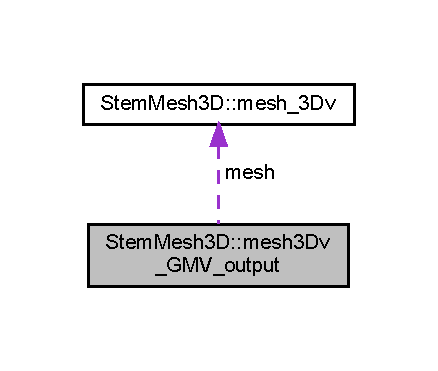
\includegraphics[width=210pt]{classStemMesh3D_1_1mesh3Dv__GMV__output__coll__graph}
\end{center}
\end{figure}
\doxysubsection*{Public Member Functions}
\begin{DoxyCompactItemize}
\item 
\mbox{\Hypertarget{classStemMesh3D_1_1mesh3Dv__GMV__output_a4ed545dca6daece2b389ef3745a6b0ef}\label{classStemMesh3D_1_1mesh3Dv__GMV__output_a4ed545dca6daece2b389ef3745a6b0ef}} 
{\bfseries mesh3\+Dv\+\_\+\+G\+M\+V\+\_\+output} (\mbox{\hyperlink{classStemMesh3D_1_1mesh__3Dv}{mesh\+\_\+3\+Dv}} \&\+\_\+mesh, size\+\_\+t \+\_\+offset=1)
\item 
\mbox{\Hypertarget{classStemMesh3D_1_1mesh3Dv__GMV__output_a557babacbbf54f53b419a70d3c2a50ff}\label{classStemMesh3D_1_1mesh3Dv__GMV__output_a557babacbbf54f53b419a70d3c2a50ff}} 
size\+\_\+t {\bfseries get\+\_\+offset} ()
\item 
\mbox{\Hypertarget{classStemMesh3D_1_1mesh3Dv__GMV__output_a2848ab52b3ba3f2c885ea7c8289bb73b}\label{classStemMesh3D_1_1mesh3Dv__GMV__output_a2848ab52b3ba3f2c885ea7c8289bb73b}} 
void {\bfseries set\+\_\+offset} (size\+\_\+t \+\_\+offset)
\item 
\mbox{\Hypertarget{classStemMesh3D_1_1mesh3Dv__GMV__output_a0fee2008918f08e40ca3cc2a88ea78ea}\label{classStemMesh3D_1_1mesh3Dv__GMV__output_a0fee2008918f08e40ca3cc2a88ea78ea}} 
virtual void {\bfseries write\+\_\+mesh} (const std\+::string \&\+\_\+fname=\char`\"{}mesh3D\char`\"{})
\item 
\mbox{\Hypertarget{classStemMesh3D_1_1mesh3Dv__GMV__output_a3419bddbef9c09ef2030aa46072c2b79}\label{classStemMesh3D_1_1mesh3Dv__GMV__output_a3419bddbef9c09ef2030aa46072c2b79}} 
virtual void {\bfseries write\+\_\+mesh} (const std\+::string \&\+\_\+fname, size\+\_\+t iR)
\end{DoxyCompactItemize}
\doxysubsection*{Protected Member Functions}
\begin{DoxyCompactItemize}
\item 
\mbox{\Hypertarget{classStemMesh3D_1_1mesh3Dv__GMV__output_ae1167b22a52e1542e94aeaba932c2968}\label{classStemMesh3D_1_1mesh3Dv__GMV__output_ae1167b22a52e1542e94aeaba932c2968}} 
void {\bfseries write\+\_\+vrtx\+\_\+data} (std\+::ostream \&file\+\_\+gmv)
\item 
\mbox{\Hypertarget{classStemMesh3D_1_1mesh3Dv__GMV__output_a4628c1d736ec019cfb3aaf946c5f32e8}\label{classStemMesh3D_1_1mesh3Dv__GMV__output_a4628c1d736ec019cfb3aaf946c5f32e8}} 
void {\bfseries write\+\_\+regn\+\_\+data} (std\+::ostream \&file\+\_\+gmv)
\item 
\mbox{\Hypertarget{classStemMesh3D_1_1mesh3Dv__GMV__output_aec46bf4128c580f140f6b9fb7ce6e53f}\label{classStemMesh3D_1_1mesh3Dv__GMV__output_aec46bf4128c580f140f6b9fb7ce6e53f}} 
void {\bfseries write\+\_\+materials} (std\+::ostream \&file\+\_\+gmv)
\item 
\mbox{\Hypertarget{classStemMesh3D_1_1mesh3Dv__GMV__output_af697ddcdff5b9fabdc00817044eac4a3}\label{classStemMesh3D_1_1mesh3Dv__GMV__output_af697ddcdff5b9fabdc00817044eac4a3}} 
void {\bfseries write\+\_\+vrtx\+\_\+data} (std\+::ostream \&file\+\_\+gmv, size\+\_\+t iR, std\+::vector$<$ size\+\_\+t $>$ \&vrtx\+\_\+idx)
\item 
\mbox{\Hypertarget{classStemMesh3D_1_1mesh3Dv__GMV__output_a0acd11a310f67e14dec3ba43614c4611}\label{classStemMesh3D_1_1mesh3Dv__GMV__output_a0acd11a310f67e14dec3ba43614c4611}} 
void {\bfseries write\+\_\+regn\+\_\+data} (std\+::ostream \&file\+\_\+gmv, size\+\_\+t iR, std\+::vector$<$ size\+\_\+t $>$ \&vrtx\+\_\+idx)
\item 
\mbox{\Hypertarget{classStemMesh3D_1_1mesh3Dv__GMV__output_acdcfd4073fb70bcb1d9b956b628bca38}\label{classStemMesh3D_1_1mesh3Dv__GMV__output_acdcfd4073fb70bcb1d9b956b628bca38}} 
void {\bfseries write\+\_\+materials} (std\+::ostream \&file\+\_\+gmv, size\+\_\+t iR)
\end{DoxyCompactItemize}
\doxysubsection*{Protected Attributes}
\begin{DoxyCompactItemize}
\item 
\mbox{\Hypertarget{classStemMesh3D_1_1mesh3Dv__GMV__output_a4e8d3c4f9b806cf4aa774de10a47ff58}\label{classStemMesh3D_1_1mesh3Dv__GMV__output_a4e8d3c4f9b806cf4aa774de10a47ff58}} 
\mbox{\hyperlink{classStemMesh3D_1_1mesh__3Dv}{mesh\+\_\+3\+Dv}} \& {\bfseries mesh}
\end{DoxyCompactItemize}


The documentation for this class was generated from the following file\+:\begin{DoxyCompactItemize}
\item 
src/\+Mesh/\+Stem\+Mesh/mesh3\+D\+\_\+\+G\+M\+V\+\_\+output.\+hh\end{DoxyCompactItemize}

\hypertarget{classStemMesh3D_1_1mesh3Dv__printer}{}\doxysection{Stem\+Mesh3D\+::mesh3\+Dv\+\_\+printer Class Reference}
\label{classStemMesh3D_1_1mesh3Dv__printer}\index{StemMesh3D::mesh3Dv\_printer@{StemMesh3D::mesh3Dv\_printer}}
\doxysubsection*{Public Member Functions}
\begin{DoxyCompactItemize}
\item 
\mbox{\Hypertarget{classStemMesh3D_1_1mesh3Dv__printer_a4490a28e0f69eb17e82f69bbecbedc91}\label{classStemMesh3D_1_1mesh3Dv__printer_a4490a28e0f69eb17e82f69bbecbedc91}} 
{\bfseries mesh3\+Dv\+\_\+printer} (\mbox{\hyperlink{classStemMesh3D_1_1mesh__3Dv}{mesh\+\_\+3\+Dv}} \&\+\_\+mesh, size\+\_\+t \+\_\+offset=0)
\item 
\mbox{\Hypertarget{classStemMesh3D_1_1mesh3Dv__printer_a32ce9cff91c8f2fcbda5420989bd8d34}\label{classStemMesh3D_1_1mesh3Dv__printer_a32ce9cff91c8f2fcbda5420989bd8d34}} 
void {\bfseries print\+\_\+\+Edge\+Vrtx} (std\+::ostream \&L\+O\+GF)
\item 
\mbox{\Hypertarget{classStemMesh3D_1_1mesh3Dv__printer_accfc89900ee983184755358302ebed2f}\label{classStemMesh3D_1_1mesh3Dv__printer_accfc89900ee983184755358302ebed2f}} 
void {\bfseries print\+\_\+\+Face\+Edge} (std\+::ostream \&L\+O\+GF)
\item 
\mbox{\Hypertarget{classStemMesh3D_1_1mesh3Dv__printer_a73fe8c6acb98dcbb29ad6acc25b6e573}\label{classStemMesh3D_1_1mesh3Dv__printer_a73fe8c6acb98dcbb29ad6acc25b6e573}} 
void {\bfseries print\+\_\+\+Regn\+Face} (std\+::ostream \&L\+O\+GF)
\item 
\mbox{\Hypertarget{classStemMesh3D_1_1mesh3Dv__printer_a1564ed9b0f2f6a303fbd66a7fcf6bd50}\label{classStemMesh3D_1_1mesh3Dv__printer_a1564ed9b0f2f6a303fbd66a7fcf6bd50}} 
void {\bfseries print\+\_\+\+Face\+Regn} (std\+::ostream \&L\+O\+GF)
\item 
\mbox{\Hypertarget{classStemMesh3D_1_1mesh3Dv__printer_a1e2b585ce0b888bfc3bf74314d8751c4}\label{classStemMesh3D_1_1mesh3Dv__printer_a1e2b585ce0b888bfc3bf74314d8751c4}} 
void {\bfseries print\+\_\+\+Edge\+Face} (std\+::ostream \&L\+O\+GF)
\item 
\mbox{\Hypertarget{classStemMesh3D_1_1mesh3Dv__printer_a93e18afee00e08ec37c4218ecc86635b}\label{classStemMesh3D_1_1mesh3Dv__printer_a93e18afee00e08ec37c4218ecc86635b}} 
void {\bfseries print\+\_\+\+Vrtx\+Edge} (std\+::ostream \&L\+O\+GF)
\item 
\mbox{\Hypertarget{classStemMesh3D_1_1mesh3Dv__printer_a9acecb2f7d8cc882fbeeed558c96dafa}\label{classStemMesh3D_1_1mesh3Dv__printer_a9acecb2f7d8cc882fbeeed558c96dafa}} 
void {\bfseries print\+\_\+boundary\+\_\+lists} (std\+::ostream \&L\+O\+GF)
\item 
\mbox{\Hypertarget{classStemMesh3D_1_1mesh3Dv__printer_a15685a631827101e81f9e73b0eb87b22}\label{classStemMesh3D_1_1mesh3Dv__printer_a15685a631827101e81f9e73b0eb87b22}} 
void {\bfseries print\+\_\+all\+\_\+datasets} ()
\item 
\mbox{\Hypertarget{classStemMesh3D_1_1mesh3Dv__printer_a632468f55de4627aab05eada804e6a3d}\label{classStemMesh3D_1_1mesh3Dv__printer_a632468f55de4627aab05eada804e6a3d}} 
void {\bfseries print\+\_\+all\+\_\+regions} ()
\item 
\mbox{\Hypertarget{classStemMesh3D_1_1mesh3Dv__printer_aea64117993d28d101debcfb51a26b849}\label{classStemMesh3D_1_1mesh3Dv__printer_aea64117993d28d101debcfb51a26b849}} 
void {\bfseries print\+\_\+region} (size\+\_\+t iR, std\+::ostream \&L\+O\+GF)
\item 
\mbox{\Hypertarget{classStemMesh3D_1_1mesh3Dv__printer_aeed1308a4db02783d52ba3927bdd2ea7}\label{classStemMesh3D_1_1mesh3Dv__printer_aeed1308a4db02783d52ba3927bdd2ea7}} 
void {\bfseries print\+\_\+all\+\_\+faces} ()
\item 
\mbox{\Hypertarget{classStemMesh3D_1_1mesh3Dv__printer_a3336da495be2683022ea12a94d18afc4}\label{classStemMesh3D_1_1mesh3Dv__printer_a3336da495be2683022ea12a94d18afc4}} 
void {\bfseries print\+\_\+face} (size\+\_\+t iF, std\+::ostream \&L\+O\+GF)
\item 
\mbox{\Hypertarget{classStemMesh3D_1_1mesh3Dv__printer_a449ed3d1409dde8bdb7013e41310b659}\label{classStemMesh3D_1_1mesh3Dv__printer_a449ed3d1409dde8bdb7013e41310b659}} 
void {\bfseries print\+\_\+all\+\_\+edges} ()
\item 
\mbox{\Hypertarget{classStemMesh3D_1_1mesh3Dv__printer_ad4bab96565bc968de82bf2854a8e8c88}\label{classStemMesh3D_1_1mesh3Dv__printer_ad4bab96565bc968de82bf2854a8e8c88}} 
void {\bfseries print\+\_\+edge} (size\+\_\+t iE, std\+::ostream \&L\+O\+GF)
\item 
\mbox{\Hypertarget{classStemMesh3D_1_1mesh3Dv__printer_aeea58049a2b09b4d1f73a2fdcca57d3e}\label{classStemMesh3D_1_1mesh3Dv__printer_aeea58049a2b09b4d1f73a2fdcca57d3e}} 
void {\bfseries print\+\_\+all\+\_\+vertices} ()
\item 
\mbox{\Hypertarget{classStemMesh3D_1_1mesh3Dv__printer_a40deea23c847da8eb426ca737d9fbb1c}\label{classStemMesh3D_1_1mesh3Dv__printer_a40deea23c847da8eb426ca737d9fbb1c}} 
void {\bfseries print\+\_\+vertex} (size\+\_\+t iV, std\+::ostream \&L\+O\+GF)
\end{DoxyCompactItemize}


The documentation for this class was generated from the following file\+:\begin{DoxyCompactItemize}
\item 
src/\+Mesh/\+Stem\+Mesh/printer.\+hh\end{DoxyCompactItemize}

\hypertarget{classStemMesh3D_1_1mesh3Dv__writer}{}\section{Stem\+Mesh3D\+:\+:mesh3\+Dv\+\_\+writer Class Reference}
\label{classStemMesh3D_1_1mesh3Dv__writer}\index{Stem\+Mesh3\+D\+::mesh3\+Dv\+\_\+writer@{Stem\+Mesh3\+D\+::mesh3\+Dv\+\_\+writer}}


Collaboration diagram for Stem\+Mesh3D\+:\+:mesh3\+Dv\+\_\+writer\+:\nopagebreak
\begin{figure}[H]
\begin{center}
\leavevmode
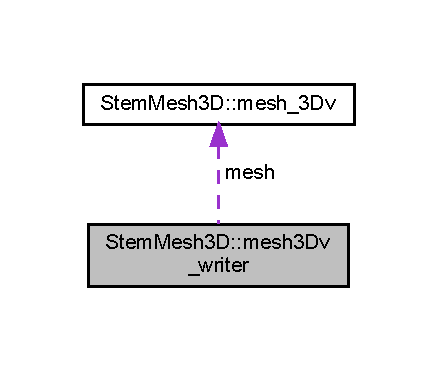
\includegraphics[width=210pt]{classStemMesh3D_1_1mesh3Dv__writer__coll__graph}
\end{center}
\end{figure}
\subsection*{Public Member Functions}
\begin{DoxyCompactItemize}
\item 
\mbox{\Hypertarget{classStemMesh3D_1_1mesh3Dv__writer_aae078d7b6c386a8b7f52ab28327caa6f}\label{classStemMesh3D_1_1mesh3Dv__writer_aae078d7b6c386a8b7f52ab28327caa6f}} 
{\bfseries mesh3\+Dv\+\_\+writer} (\hyperlink{classStemMesh3D_1_1mesh__3Dv}{mesh\+\_\+3\+Dv} \&\+\_\+mesh, size\+\_\+t \+\_\+offset=0)
\item 
\mbox{\Hypertarget{classStemMesh3D_1_1mesh3Dv__writer_aa52af5320c8e803cd545dda23fcabb35}\label{classStemMesh3D_1_1mesh3Dv__writer_aa52af5320c8e803cd545dda23fcabb35}} 
void {\bfseries write\+\_\+mesh\+\_\+\+RF} (const std\+::string \&fname=\char`\"{}mesh3D\char`\"{})
\item 
\mbox{\Hypertarget{classStemMesh3D_1_1mesh3Dv__writer_a0f9451cb63615486da604d9fd4f5e81e}\label{classStemMesh3D_1_1mesh3Dv__writer_a0f9451cb63615486da604d9fd4f5e81e}} 
void {\bfseries write\+\_\+mesh\+\_\+\+Fb} (const std\+::string \&fname=\char`\"{}mesh3D\char`\"{})
\item 
\mbox{\Hypertarget{classStemMesh3D_1_1mesh3Dv__writer_adb50b614cf1af342128afa716453837e}\label{classStemMesh3D_1_1mesh3Dv__writer_adb50b614cf1af342128afa716453837e}} 
void {\bfseries write\+\_\+mesh\+\_\+\+M\+SH} (const std\+::string \&fname=\char`\"{}mesh3D\char`\"{})
\item 
\mbox{\Hypertarget{classStemMesh3D_1_1mesh3Dv__writer_af2db4004e9f0914b373757bec47bbc3b}\label{classStemMesh3D_1_1mesh3Dv__writer_af2db4004e9f0914b373757bec47bbc3b}} 
void {\bfseries write\+\_\+node\+\_\+coords\+\_\+\+Suku\+\_\+format} (const std\+::string \&fname)
\item 
\mbox{\Hypertarget{classStemMesh3D_1_1mesh3Dv__writer_aa38443a40c4c444704ff4d04de6299c6}\label{classStemMesh3D_1_1mesh3Dv__writer_aa38443a40c4c444704ff4d04de6299c6}} 
void {\bfseries write\+\_\+mesh\+\_\+\+R\+F\+\_\+\+Suku\+\_\+format} (const std\+::string \&fname)
\item 
\mbox{\Hypertarget{classStemMesh3D_1_1mesh3Dv__writer_ad48372d1a5e4b4de2487495da624c790}\label{classStemMesh3D_1_1mesh3Dv__writer_ad48372d1a5e4b4de2487495da624c790}} 
size\+\_\+t {\bfseries get\+\_\+offset} ()
\item 
\mbox{\Hypertarget{classStemMesh3D_1_1mesh3Dv__writer_abd36bcea35434ec6be611efd550d91e8}\label{classStemMesh3D_1_1mesh3Dv__writer_abd36bcea35434ec6be611efd550d91e8}} 
void {\bfseries set\+\_\+offset} (size\+\_\+t \+\_\+offset)
\end{DoxyCompactItemize}
\subsection*{Protected Member Functions}
\begin{DoxyCompactItemize}
\item 
\mbox{\Hypertarget{classStemMesh3D_1_1mesh3Dv__writer_aa3954191960a61dd2aed64d4a1639352}\label{classStemMesh3D_1_1mesh3Dv__writer_aa3954191960a61dd2aed64d4a1639352}} 
void {\bfseries write\+\_\+node\+\_\+coords} (const std\+::string \&fname=\char`\"{}mesh3D\char`\"{})
\end{DoxyCompactItemize}
\subsection*{Protected Attributes}
\begin{DoxyCompactItemize}
\item 
\mbox{\Hypertarget{classStemMesh3D_1_1mesh3Dv__writer_afcc6928486dd97041191366ab9c35c8e}\label{classStemMesh3D_1_1mesh3Dv__writer_afcc6928486dd97041191366ab9c35c8e}} 
\hyperlink{classStemMesh3D_1_1mesh__3Dv}{mesh\+\_\+3\+Dv} \& {\bfseries mesh}
\item 
\mbox{\Hypertarget{classStemMesh3D_1_1mesh3Dv__writer_af734b616320e49709b8797e779fe2798}\label{classStemMesh3D_1_1mesh3Dv__writer_af734b616320e49709b8797e779fe2798}} 
size\+\_\+t {\bfseries offset}
\item 
\mbox{\Hypertarget{classStemMesh3D_1_1mesh3Dv__writer_aa38a6f6f2f6fc20303589aea01af02ce}\label{classStemMesh3D_1_1mesh3Dv__writer_aa38a6f6f2f6fc20303589aea01af02ce}} 
size\+\_\+t {\bfseries n\+\_\+vflag}
\item 
\mbox{\Hypertarget{classStemMesh3D_1_1mesh3Dv__writer_a40016c367f564af223b7b5a24b265eaa}\label{classStemMesh3D_1_1mesh3Dv__writer_a40016c367f564af223b7b5a24b265eaa}} 
size\+\_\+t {\bfseries n\+\_\+fflag}
\item 
\mbox{\Hypertarget{classStemMesh3D_1_1mesh3Dv__writer_a521af78f761e436e82fcffa050bca58f}\label{classStemMesh3D_1_1mesh3Dv__writer_a521af78f761e436e82fcffa050bca58f}} 
size\+\_\+t {\bfseries n\+\_\+rflag}
\end{DoxyCompactItemize}
\subsection*{Static Protected Attributes}
\begin{DoxyCompactItemize}
\item 
\mbox{\Hypertarget{classStemMesh3D_1_1mesh3Dv__writer_ac3a19a51146235a50852d73bb2593ff2}\label{classStemMesh3D_1_1mesh3Dv__writer_ac3a19a51146235a50852d73bb2593ff2}} 
static const size\+\_\+t {\bfseries D\+IM} = 3
\end{DoxyCompactItemize}


The documentation for this class was generated from the following file\+:\begin{DoxyCompactItemize}
\item 
src/\+Mesh/\+Stem\+Mesh/mesh3\+D\+\_\+writer.\+hh\end{DoxyCompactItemize}

\hypertarget{classStemMesh3D_1_1mesh3Dv__writer__MSH}{}\doxysection{Stem\+Mesh3D\+::mesh3\+Dv\+\_\+writer\+\_\+\+M\+SH Class Reference}
\label{classStemMesh3D_1_1mesh3Dv__writer__MSH}\index{StemMesh3D::mesh3Dv\_writer\_MSH@{StemMesh3D::mesh3Dv\_writer\_MSH}}


Collaboration diagram for Stem\+Mesh3D\+::mesh3\+Dv\+\_\+writer\+\_\+\+M\+SH\+:\nopagebreak
\begin{figure}[H]
\begin{center}
\leavevmode
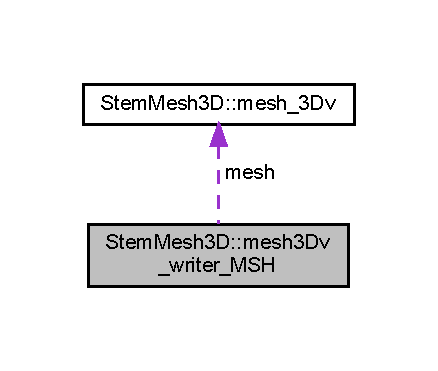
\includegraphics[width=210pt]{classStemMesh3D_1_1mesh3Dv__writer__MSH__coll__graph}
\end{center}
\end{figure}
\doxysubsection*{Public Member Functions}
\begin{DoxyCompactItemize}
\item 
\mbox{\Hypertarget{classStemMesh3D_1_1mesh3Dv__writer__MSH_addc534a27959ee5278aaa44dba796cb2}\label{classStemMesh3D_1_1mesh3Dv__writer__MSH_addc534a27959ee5278aaa44dba796cb2}} 
{\bfseries mesh3\+Dv\+\_\+writer\+\_\+\+M\+SH} (\mbox{\hyperlink{classStemMesh3D_1_1mesh__3Dv}{mesh\+\_\+3\+Dv}} \&\+\_\+mesh, size\+\_\+t \+\_\+offset=1)
\item 
\mbox{\Hypertarget{classStemMesh3D_1_1mesh3Dv__writer__MSH_a1293667146a6678f0667720da49bae80}\label{classStemMesh3D_1_1mesh3Dv__writer__MSH_a1293667146a6678f0667720da49bae80}} 
void {\bfseries write\+\_\+header} (std\+::ostream \&O\+U\+TF, const std\+::string \&mesh\+\_\+name\+\_\+str)
\item 
\mbox{\Hypertarget{classStemMesh3D_1_1mesh3Dv__writer__MSH_a2bd955e2ef48ba27f6b72558588a2746}\label{classStemMesh3D_1_1mesh3Dv__writer__MSH_a2bd955e2ef48ba27f6b72558588a2746}} 
void {\bfseries write\+\_\+coords} (std\+::ostream \&O\+U\+TF)
\item 
\mbox{\Hypertarget{classStemMesh3D_1_1mesh3Dv__writer__MSH_a60dfc86cab83e01b0f1e768d79433dad}\label{classStemMesh3D_1_1mesh3Dv__writer__MSH_a60dfc86cab83e01b0f1e768d79433dad}} 
void {\bfseries write\+\_\+\+Regn\+Face} (std\+::ostream \&O\+U\+TF)
\item 
\mbox{\Hypertarget{classStemMesh3D_1_1mesh3Dv__writer__MSH_a9a88a2cf4473c0903ade42135985272c}\label{classStemMesh3D_1_1mesh3Dv__writer__MSH_a9a88a2cf4473c0903ade42135985272c}} 
void {\bfseries write\+\_\+\+Regn\+Vrtx} (std\+::ostream \&O\+U\+TF)
\item 
\mbox{\Hypertarget{classStemMesh3D_1_1mesh3Dv__writer__MSH_a4c0bbe0405b2cf3a76fc2f2f68e7633d}\label{classStemMesh3D_1_1mesh3Dv__writer__MSH_a4c0bbe0405b2cf3a76fc2f2f68e7633d}} 
void {\bfseries write\+\_\+\+Face\+Edge} (std\+::ostream \&O\+U\+TF)
\item 
\mbox{\Hypertarget{classStemMesh3D_1_1mesh3Dv__writer__MSH_a4caa9456d10177cbc59cbc5d6e442f50}\label{classStemMesh3D_1_1mesh3Dv__writer__MSH_a4caa9456d10177cbc59cbc5d6e442f50}} 
void {\bfseries write\+\_\+\+Face\+Vrtx} (std\+::ostream \&O\+U\+TF)
\item 
\mbox{\Hypertarget{classStemMesh3D_1_1mesh3Dv__writer__MSH_a87b07b5d20ba5f2899d8b441f4509540}\label{classStemMesh3D_1_1mesh3Dv__writer__MSH_a87b07b5d20ba5f2899d8b441f4509540}} 
void {\bfseries write\+\_\+\+Face\+Regn} (std\+::ostream \&O\+U\+TF)
\item 
\mbox{\Hypertarget{classStemMesh3D_1_1mesh3Dv__writer__MSH_abe2c47741626aac00a659cac21f1fbc7}\label{classStemMesh3D_1_1mesh3Dv__writer__MSH_abe2c47741626aac00a659cac21f1fbc7}} 
void {\bfseries write\+\_\+\+Edge\+Vrtx} (std\+::ostream \&O\+U\+TF)
\item 
\mbox{\Hypertarget{classStemMesh3D_1_1mesh3Dv__writer__MSH_afdf5e70b8a6edf803c2e45083ae3b489}\label{classStemMesh3D_1_1mesh3Dv__writer__MSH_afdf5e70b8a6edf803c2e45083ae3b489}} 
void {\bfseries write\+\_\+mesh\+\_\+\+M\+SH} (const std\+::string \&fname=\char`\"{}mesh3D\char`\"{})
\end{DoxyCompactItemize}
\doxysubsection*{Protected Types}
\begin{DoxyCompactItemize}
\item 
\mbox{\Hypertarget{classStemMesh3D_1_1mesh3Dv__writer__MSH_a7bcfd46c78fab12ebec84b739f8f2a6d}\label{classStemMesh3D_1_1mesh3Dv__writer__MSH_a7bcfd46c78fab12ebec84b739f8f2a6d}} 
enum {\bfseries Language} \{ {\bfseries F\+R\+E\+N\+CH}, 
{\bfseries E\+N\+G\+L\+I\+SH}
 \}
\end{DoxyCompactItemize}
\doxysubsection*{Protected Attributes}
\begin{DoxyCompactItemize}
\item 
\mbox{\Hypertarget{classStemMesh3D_1_1mesh3Dv__writer__MSH_ab86ffc519fc1287ee962f32339e5bf46}\label{classStemMesh3D_1_1mesh3Dv__writer__MSH_ab86ffc519fc1287ee962f32339e5bf46}} 
\mbox{\hyperlink{classStemMesh3D_1_1mesh__3Dv}{mesh\+\_\+3\+Dv}} \& {\bfseries mesh}
\item 
\mbox{\Hypertarget{classStemMesh3D_1_1mesh3Dv__writer__MSH_a29f02c87b8e232aa8f6dac83ece95c7d}\label{classStemMesh3D_1_1mesh3Dv__writer__MSH_a29f02c87b8e232aa8f6dac83ece95c7d}} 
const size\+\_\+t {\bfseries offset}
\item 
\mbox{\Hypertarget{classStemMesh3D_1_1mesh3Dv__writer__MSH_aa5695d61e0cd3c4fb7da6f8779eef643}\label{classStemMesh3D_1_1mesh3Dv__writer__MSH_aa5695d61e0cd3c4fb7da6f8779eef643}} 
const Language {\bfseries lang\+\_\+flag}
\end{DoxyCompactItemize}


The documentation for this class was generated from the following file\+:\begin{DoxyCompactItemize}
\item 
src/\+Mesh/\+Stem\+Mesh/mesh3\+D\+\_\+writer.\+hh\end{DoxyCompactItemize}

\hypertarget{classStemMesh3D_1_1mesh__3Dv}{}\section{Stem\+Mesh3D\+:\+:mesh\+\_\+3\+Dv Class Reference}
\label{classStemMesh3D_1_1mesh__3Dv}\index{Stem\+Mesh3\+D\+::mesh\+\_\+3\+Dv@{Stem\+Mesh3\+D\+::mesh\+\_\+3\+Dv}}


The interface for working with generic 3D meshes.  




{\ttfamily \#include $<$mesh3\+D.\+hh$>$}

\subsection*{Public Types}
\begin{DoxyCompactItemize}
\item 
\mbox{\Hypertarget{classStemMesh3D_1_1mesh__3Dv_a550002922df52cb0711f6d0da2398d6b}\label{classStemMesh3D_1_1mesh__3Dv_a550002922df52cb0711f6d0da2398d6b}} 
enum \hyperlink{classStemMesh3D_1_1mesh__3Dv_a550002922df52cb0711f6d0da2398d6b}{bbox\+\_\+dimension} \{ \newline
{\bfseries xmin}, 
{\bfseries ymin}, 
{\bfseries zmin}, 
{\bfseries xmax}, 
\newline
{\bfseries ymax}, 
{\bfseries zmax}
 \}\begin{DoxyCompactList}\small\item\em The six extremes of the bounding box of the domain. \end{DoxyCompactList}
\item 
\mbox{\Hypertarget{classStemMesh3D_1_1mesh__3Dv_a9544cba555b60f17f04fcd1689314338}\label{classStemMesh3D_1_1mesh__3Dv_a9544cba555b60f17f04fcd1689314338}} 
using \hyperlink{classStemMesh3D_1_1mesh__3Dv_a9544cba555b60f17f04fcd1689314338}{flag\+\_\+type} = int
\begin{DoxyCompactList}\small\item\em Type used for element flags. \end{DoxyCompactList}\end{DoxyCompactItemize}
\subsection*{Public Member Functions}
\begin{DoxyCompactItemize}
\item 
\mbox{\Hypertarget{classStemMesh3D_1_1mesh__3Dv_ab7799362e99de42d7fef62d12f007367}\label{classStemMesh3D_1_1mesh__3Dv_ab7799362e99de42d7fef62d12f007367}} 
size\+\_\+t \hyperlink{classStemMesh3D_1_1mesh__3Dv_ab7799362e99de42d7fef62d12f007367}{n\+\_\+region} () const
\begin{DoxyCompactList}\small\item\em Returns the number of regions (3D cells / control volumes) in the mesh. \end{DoxyCompactList}\item 
\mbox{\Hypertarget{classStemMesh3D_1_1mesh__3Dv_a06d9c5f13b364627149ea844501e9441}\label{classStemMesh3D_1_1mesh__3Dv_a06d9c5f13b364627149ea844501e9441}} 
size\+\_\+t \hyperlink{classStemMesh3D_1_1mesh__3Dv_a06d9c5f13b364627149ea844501e9441}{n\+\_\+face} () const
\begin{DoxyCompactList}\small\item\em Returns the number of faces in the mesh. \end{DoxyCompactList}\item 
\mbox{\Hypertarget{classStemMesh3D_1_1mesh__3Dv_a8068061ffd6a9080b92d25270c1f668d}\label{classStemMesh3D_1_1mesh__3Dv_a8068061ffd6a9080b92d25270c1f668d}} 
size\+\_\+t \hyperlink{classStemMesh3D_1_1mesh__3Dv_a8068061ffd6a9080b92d25270c1f668d}{n\+\_\+edge} () const
\begin{DoxyCompactList}\small\item\em Returns the number of edges in the mesh/. \end{DoxyCompactList}\item 
\mbox{\Hypertarget{classStemMesh3D_1_1mesh__3Dv_ac29b66e58fbd9bc301118bea14426709}\label{classStemMesh3D_1_1mesh__3Dv_ac29b66e58fbd9bc301118bea14426709}} 
size\+\_\+t \hyperlink{classStemMesh3D_1_1mesh__3Dv_ac29b66e58fbd9bc301118bea14426709}{n\+\_\+vertex} () const
\begin{DoxyCompactList}\small\item\em Returns the number of vertices in the mesh. \end{DoxyCompactList}\item 
\mbox{\Hypertarget{classStemMesh3D_1_1mesh__3Dv_a7c885048a027fc84eb6d2b7e2590c5e2}\label{classStemMesh3D_1_1mesh__3Dv_a7c885048a027fc84eb6d2b7e2590c5e2}} 
size\+\_\+t \hyperlink{classStemMesh3D_1_1mesh__3Dv_a7c885048a027fc84eb6d2b7e2590c5e2}{n\+\_\+bregion} () const
\begin{DoxyCompactList}\small\item\em Returns the number of regions on the boundary. \end{DoxyCompactList}\item 
\mbox{\Hypertarget{classStemMesh3D_1_1mesh__3Dv_a394bc87d5f29715e6faae1e2d21ceff7}\label{classStemMesh3D_1_1mesh__3Dv_a394bc87d5f29715e6faae1e2d21ceff7}} 
size\+\_\+t \hyperlink{classStemMesh3D_1_1mesh__3Dv_a394bc87d5f29715e6faae1e2d21ceff7}{n\+\_\+bface} () const
\begin{DoxyCompactList}\small\item\em Returns the number of faces on the boundary. \end{DoxyCompactList}\item 
\mbox{\Hypertarget{classStemMesh3D_1_1mesh__3Dv_aa9793810147053ffdfcd9cc9eeaec160}\label{classStemMesh3D_1_1mesh__3Dv_aa9793810147053ffdfcd9cc9eeaec160}} 
size\+\_\+t \hyperlink{classStemMesh3D_1_1mesh__3Dv_aa9793810147053ffdfcd9cc9eeaec160}{n\+\_\+bedge} () const
\begin{DoxyCompactList}\small\item\em Returns the number of edges on the boundary. \end{DoxyCompactList}\item 
\mbox{\Hypertarget{classStemMesh3D_1_1mesh__3Dv_a616550f2a459b5c239d2d205a408b484}\label{classStemMesh3D_1_1mesh__3Dv_a616550f2a459b5c239d2d205a408b484}} 
size\+\_\+t \hyperlink{classStemMesh3D_1_1mesh__3Dv_a616550f2a459b5c239d2d205a408b484}{n\+\_\+bvertex} () const
\begin{DoxyCompactList}\small\item\em Returns the number of vertices on the boundary. \end{DoxyCompactList}\item 
size\+\_\+t \hyperlink{classStemMesh3D_1_1mesh__3Dv_a91cb00af3bac18dbde6320e4178111ed}{get\+\_\+bnd\+\_\+regn} (size\+\_\+t ilR) const
\begin{DoxyCompactList}\small\item\em Returns the global region number of the (ilR)\textquotesingle{}th boundary region. \end{DoxyCompactList}\item 
size\+\_\+t \hyperlink{classStemMesh3D_1_1mesh__3Dv_a990498932160b3031badb906be06fb84}{get\+\_\+bnd\+\_\+face} (size\+\_\+t ilF) const
\begin{DoxyCompactList}\small\item\em Returns the global face number of the (ilF)\textquotesingle{}th boundary face. \end{DoxyCompactList}\item 
size\+\_\+t \hyperlink{classStemMesh3D_1_1mesh__3Dv_a329a4b4f0ae621e3a700c61d52f82fdd}{get\+\_\+bnd\+\_\+edge} (size\+\_\+t ilE) const
\begin{DoxyCompactList}\small\item\em Returns the global edge number of the (ilE)\textquotesingle{}th boundary edge. \end{DoxyCompactList}\item 
size\+\_\+t \hyperlink{classStemMesh3D_1_1mesh__3Dv_a397ec757e2e38525d7a9721112f6a08a}{get\+\_\+bnd\+\_\+vrtx} (size\+\_\+t ilV) const
\begin{DoxyCompactList}\small\item\em Returns the global vertex number of the (ilV)\textquotesingle{}th boundary vertex. \end{DoxyCompactList}\item 
size\+\_\+t \hyperlink{classStemMesh3D_1_1mesh__3Dv_a761e6d7a78b1547681310935e1ce0a8c}{regn\+\_\+face} (size\+\_\+t iR, size\+\_\+t ilF) const
\begin{DoxyCompactList}\small\item\em Returns the global face number of the (ilF)\textquotesingle{}th local face of the region iR. \end{DoxyCompactList}\item 
size\+\_\+t \hyperlink{classStemMesh3D_1_1mesh__3Dv_a70f328491a6660c05914c9226e297ecc}{face\+\_\+edge} (size\+\_\+t iF, size\+\_\+t ilE) const
\begin{DoxyCompactList}\small\item\em Returns the global edge number of the (ilE)\textquotesingle{}th local edge of the face iF. \end{DoxyCompactList}\item 
size\+\_\+t \hyperlink{classStemMesh3D_1_1mesh__3Dv_a7024d4e9bd97ff05c7926c9b4a97be62}{edge\+\_\+vrtx} (size\+\_\+t iE, size\+\_\+t ilV) const
\begin{DoxyCompactList}\small\item\em Returns the global vertex number of the (ilV)\textquotesingle{}th vertex of the edge iE. \end{DoxyCompactList}\item 
size\+\_\+t \hyperlink{classStemMesh3D_1_1mesh__3Dv_afd4c48e4133adad4c31e6fe8bfb96c2a}{face\+\_\+regn} (size\+\_\+t iF, size\+\_\+t ilR) const
\begin{DoxyCompactList}\small\item\em Returns the global region number of the (ilR)\textquotesingle{}th region bordering the face iF. \end{DoxyCompactList}\item 
size\+\_\+t \hyperlink{classStemMesh3D_1_1mesh__3Dv_aef749900ff2a72c8dbb21b28f3c21556}{edge\+\_\+face} (size\+\_\+t iE, size\+\_\+t ilF) const
\begin{DoxyCompactList}\small\item\em Returns the global face number of the (ilF)\textquotesingle{}th face bordering the edge iE. \end{DoxyCompactList}\item 
size\+\_\+t \hyperlink{classStemMesh3D_1_1mesh__3Dv_a93fff194e371aa21a00f0e5e1e6d45cd}{vrtx\+\_\+edge} (size\+\_\+t iV, size\+\_\+t ilE) const
\begin{DoxyCompactList}\small\item\em Returns the global edge number of the (ilE)\textquotesingle{}th edge adjacent to the vertex iV. \end{DoxyCompactList}\item 
size\+\_\+t \hyperlink{classStemMesh3D_1_1mesh__3Dv_afbe4f73847a1ae2c6a24170ab3a7827e}{vrtx\+\_\+vrtx} (size\+\_\+t iV, size\+\_\+t ilV) const
\begin{DoxyCompactList}\small\item\em Returns the global vertex number of the (ilV)\textquotesingle{}th adjacent vertex to vertex iV. \end{DoxyCompactList}\item 
size\+\_\+t \hyperlink{classStemMesh3D_1_1mesh__3Dv_a02974473e896bc49a5a19cd92b521061}{n\+\_\+regn\+\_\+face} (size\+\_\+t iR) const
\begin{DoxyCompactList}\small\item\em Returns the number of local faces that are adjacent to the given region. \end{DoxyCompactList}\item 
size\+\_\+t \hyperlink{classStemMesh3D_1_1mesh__3Dv_a2d8ae772da1e33edfb9332823d4c7212}{n\+\_\+face\+\_\+edge} (size\+\_\+t iF) const
\begin{DoxyCompactList}\small\item\em Returns the number of local edges that are adjacent to the given face. \end{DoxyCompactList}\item 
size\+\_\+t \hyperlink{classStemMesh3D_1_1mesh__3Dv_a3a0580ffb017ad1118c6b10631b845fb}{n\+\_\+edge\+\_\+vrtx} (size\+\_\+t iE) const
\begin{DoxyCompactList}\small\item\em Returns the number of local vertices that are adjacent to the given edge. This should always return 2. \end{DoxyCompactList}\item 
size\+\_\+t \hyperlink{classStemMesh3D_1_1mesh__3Dv_a121da582c92b922a0d6ca76a0f1330ee}{n\+\_\+face\+\_\+regn} (size\+\_\+t iF) const
\begin{DoxyCompactList}\small\item\em Returns the number of regions that are adjacent to the given face. \end{DoxyCompactList}\item 
size\+\_\+t \hyperlink{classStemMesh3D_1_1mesh__3Dv_a7655cc55bc89437d85f1a7beddbf66f4}{n\+\_\+edge\+\_\+face} (size\+\_\+t iE) const
\begin{DoxyCompactList}\small\item\em Returns the number of faces that are adjacent to the given edge. \end{DoxyCompactList}\item 
size\+\_\+t \hyperlink{classStemMesh3D_1_1mesh__3Dv_a9996181afbb34b235ef0877471eb4fb3}{n\+\_\+vrtx\+\_\+edge} (size\+\_\+t iV) const
\begin{DoxyCompactList}\small\item\em Returns the number of edges that are adjacent to the given vertex. \end{DoxyCompactList}\item 
size\+\_\+t \hyperlink{classStemMesh3D_1_1mesh__3Dv_a1a6eaa9ed8ebf41ada912b834f34e7c6}{n\+\_\+vrtx\+\_\+vrtx} (size\+\_\+t iV) const
\begin{DoxyCompactList}\small\item\em Returns the number of vertices that are adjacent to the given vertex. \end{DoxyCompactList}\item 
bool \hyperlink{classStemMesh3D_1_1mesh__3Dv_a4c6ab11bf9ea2eac1709052d14f5c5b3}{ok\+\_\+regn\+\_\+face} (size\+\_\+t iR, size\+\_\+t ilF) const
\begin{DoxyCompactList}\small\item\em Returns true if the global face corresponding to ilF is oriented correctly with respect to iR. \end{DoxyCompactList}\item 
bool \hyperlink{classStemMesh3D_1_1mesh__3Dv_af49e94aea3119432fadf9878cafba5c5}{ok\+\_\+face\+\_\+edge} (size\+\_\+t iF, size\+\_\+t ilE) const
\begin{DoxyCompactList}\small\item\em Returns true if the global edge corresponding to ilE is oriented correctly with respect to iF. \end{DoxyCompactList}\item 
bool \hyperlink{classStemMesh3D_1_1mesh__3Dv_a0864ac0c5e4a946ff620caf60ba2526e}{ok\+\_\+edge\+\_\+face} (size\+\_\+t iE, size\+\_\+t ilF) const
\begin{DoxyCompactList}\small\item\em Returns true if the global face corresponding to ilF is oriented correctly with respect to iE. \end{DoxyCompactList}\item 
bool \hyperlink{classStemMesh3D_1_1mesh__3Dv_a1bcbb55c1a867e69c088f13ce09f924f}{ok\+\_\+vrtx\+\_\+edge} (size\+\_\+t iV, size\+\_\+t ilE) const
\begin{DoxyCompactList}\small\item\em Returns true if the global vertex iV is the first vertex on the global edge corresponding to ilE. \end{DoxyCompactList}\item 
void \hyperlink{classStemMesh3D_1_1mesh__3Dv_aae9d1d4fa2441cb2ac8e6a05f3e5038b}{get\+\_\+regn\+\_\+regn} (size\+\_\+t iR, std\+::vector$<$ size\+\_\+t $>$ \&rlist) const
\begin{DoxyCompactList}\small\item\em Populate the given vector with the region numbers of all regions adjacent to the given region. \end{DoxyCompactList}\item 
void \hyperlink{classStemMesh3D_1_1mesh__3Dv_a7388f79d9b639140efda17e33d169547}{get\+\_\+regn\+\_\+face} (size\+\_\+t iR, std\+::vector$<$ size\+\_\+t $>$ \&flist) const
\begin{DoxyCompactList}\small\item\em Populate the given vector with the face numbers of all faces adjacent to the given region. \end{DoxyCompactList}\item 
void \hyperlink{classStemMesh3D_1_1mesh__3Dv_a9a60d9a26cb41402390b0acc5cbd17ec}{get\+\_\+regn\+\_\+edge} (size\+\_\+t iR, std\+::vector$<$ size\+\_\+t $>$ \&elist) const
\begin{DoxyCompactList}\small\item\em Populate the given vector with the edge numbers of all edges adjacent to the given region. \end{DoxyCompactList}\item 
void \hyperlink{classStemMesh3D_1_1mesh__3Dv_a063d41ebed2be9a826b8254f38a0c7d9}{get\+\_\+regn\+\_\+vrtx} (size\+\_\+t iR, std\+::vector$<$ size\+\_\+t $>$ \&vlist) const
\begin{DoxyCompactList}\small\item\em Populate the given vector with the vertex numbers of all vertices adjacent to the given region. \end{DoxyCompactList}\item 
void \hyperlink{classStemMesh3D_1_1mesh__3Dv_a77ba74ed0585df27c1d16b26d2a4caa0}{get\+\_\+face\+\_\+regn} (size\+\_\+t iF, std\+::vector$<$ size\+\_\+t $>$ \&rlist) const
\begin{DoxyCompactList}\small\item\em Populate the given vector with the region numbers of all regions adjacent to the given face. \end{DoxyCompactList}\item 
void \hyperlink{classStemMesh3D_1_1mesh__3Dv_ab505aac621d73bedfb3f7145ee857054}{get\+\_\+face\+\_\+face} (size\+\_\+t iF, std\+::vector$<$ size\+\_\+t $>$ \&flist) const
\begin{DoxyCompactList}\small\item\em Populate the given vector with the face numbers of all faces adjacent to the given face. \end{DoxyCompactList}\item 
void \hyperlink{classStemMesh3D_1_1mesh__3Dv_ae1cecbb86f79a41a6e979e6afc32be3f}{get\+\_\+face\+\_\+edge} (size\+\_\+t iF, std\+::vector$<$ size\+\_\+t $>$ \&elist) const
\begin{DoxyCompactList}\small\item\em Populate the given vector with the edge numbers of all edges adjacent to the given face. \end{DoxyCompactList}\item 
void \hyperlink{classStemMesh3D_1_1mesh__3Dv_a4a48a14ef16c33c441fff9dafd26989b}{get\+\_\+face\+\_\+vrtx} (size\+\_\+t iF, std\+::vector$<$ size\+\_\+t $>$ \&vlist) const
\begin{DoxyCompactList}\small\item\em Populate the given vector with the vertex numbers of all vertices adjacent to the given face. \end{DoxyCompactList}\item 
void \hyperlink{classStemMesh3D_1_1mesh__3Dv_ace07d45b45e79fd62e37530b6e5501c8}{get\+\_\+edge\+\_\+regn} (size\+\_\+t iE, std\+::vector$<$ size\+\_\+t $>$ \&rlist) const
\begin{DoxyCompactList}\small\item\em Populate the given vector with the region numbers of all regions adjacent to the given edge. \end{DoxyCompactList}\item 
void \hyperlink{classStemMesh3D_1_1mesh__3Dv_acfc3f5d372d82b08180391776e0e5b85}{get\+\_\+edge\+\_\+face} (size\+\_\+t iE, std\+::vector$<$ size\+\_\+t $>$ \&flist) const
\begin{DoxyCompactList}\small\item\em Populate the given vector with the face numbers of all faces adjacent to the given edge. \end{DoxyCompactList}\item 
void \hyperlink{classStemMesh3D_1_1mesh__3Dv_a06babc4d9918195a426c4800dec47979}{get\+\_\+edge\+\_\+edge} (size\+\_\+t iE, std\+::vector$<$ size\+\_\+t $>$ \&elist) const
\begin{DoxyCompactList}\small\item\em Populate the given vector with the edge numbers of all edges adjacent to the given edge. \end{DoxyCompactList}\item 
void \hyperlink{classStemMesh3D_1_1mesh__3Dv_ab815cec3c06264372a7e57e01e1db380}{get\+\_\+edge\+\_\+vrtx} (size\+\_\+t iE, std\+::vector$<$ size\+\_\+t $>$ \&vlist) const
\begin{DoxyCompactList}\small\item\em Populate the given vector with the vertex numbers of all vertices adjacent to the given edge. \end{DoxyCompactList}\item 
void \hyperlink{classStemMesh3D_1_1mesh__3Dv_a39a03b8697cda8c74485cfc118299eea}{get\+\_\+vrtx\+\_\+regn} (size\+\_\+t iV, std\+::vector$<$ size\+\_\+t $>$ \&rlist) const
\begin{DoxyCompactList}\small\item\em Populate the given vector with the region numbers of all regions adjacent to the given vertex. \end{DoxyCompactList}\item 
void \hyperlink{classStemMesh3D_1_1mesh__3Dv_a75a75c96ae9daf80877c60480020667a}{get\+\_\+vrtx\+\_\+face} (size\+\_\+t iV, std\+::vector$<$ size\+\_\+t $>$ \&flist) const
\begin{DoxyCompactList}\small\item\em Populate the given vector with the face numbers of all faces adjacent to the given vertex. \end{DoxyCompactList}\item 
void \hyperlink{classStemMesh3D_1_1mesh__3Dv_aa5e678364abe37ff90930374d706cf6f}{get\+\_\+vrtx\+\_\+edge} (size\+\_\+t iV, std\+::vector$<$ size\+\_\+t $>$ \&elist) const
\begin{DoxyCompactList}\small\item\em Populate the given vector with the edge numbers of all edges adjacent to the given vertex. \end{DoxyCompactList}\item 
void \hyperlink{classStemMesh3D_1_1mesh__3Dv_ae06da20fca1682cf92dd808f2880517f}{get\+\_\+vrtx\+\_\+vrtx} (size\+\_\+t iV, std\+::vector$<$ size\+\_\+t $>$ \&vlist) const
\begin{DoxyCompactList}\small\item\em Populate the given vector with the vertex numbers of all vertices adjacent to the given vertex. \end{DoxyCompactList}\item 
bool \hyperlink{classStemMesh3D_1_1mesh__3Dv_aa6ba589981c83feda412066fd0580032}{is\+\_\+boundary\+\_\+vrtx} (size\+\_\+t iV) const
\begin{DoxyCompactList}\small\item\em Returns true if the vertex with the given number is on the boundary. \end{DoxyCompactList}\item 
bool \hyperlink{classStemMesh3D_1_1mesh__3Dv_ae947ad7de0dffd404d5641467bc5fee4}{is\+\_\+boundary\+\_\+edge} (size\+\_\+t iE) const
\begin{DoxyCompactList}\small\item\em Returns true if the edge with the given number is on the boundary. \end{DoxyCompactList}\item 
bool \hyperlink{classStemMesh3D_1_1mesh__3Dv_a3c02e5034f9c9e08ae91057fb165fbad}{is\+\_\+boundary\+\_\+face} (size\+\_\+t iF) const
\begin{DoxyCompactList}\small\item\em Returns true if the face with the given number is on the boundary. \end{DoxyCompactList}\item 
bool \hyperlink{classStemMesh3D_1_1mesh__3Dv_a3c3a3d3014b5e7d097facf759364f6a7}{is\+\_\+boundary\+\_\+regn} (size\+\_\+t iR) const
\begin{DoxyCompactList}\small\item\em Returns true if the region with the given number is on the boundary. \end{DoxyCompactList}\item 
bool \hyperlink{classStemMesh3D_1_1mesh__3Dv_aa7dc342e2b241b485f5a5f8f722e660f}{is\+\_\+internal\+\_\+vrtx} (size\+\_\+t iV) const
\begin{DoxyCompactList}\small\item\em Returns true if the vertex with the given number is internal (not on the boundary) \end{DoxyCompactList}\item 
bool \hyperlink{classStemMesh3D_1_1mesh__3Dv_ae4e6b4995cb4169fdb930a508d0b83de}{is\+\_\+internal\+\_\+edge} (size\+\_\+t iE) const
\begin{DoxyCompactList}\small\item\em Returns true if the edge with the given number is internal (not on the boundary) \end{DoxyCompactList}\item 
bool \hyperlink{classStemMesh3D_1_1mesh__3Dv_a7ec74c519a65b29f52e243e4905b687d}{is\+\_\+internal\+\_\+face} (size\+\_\+t iF) const
\begin{DoxyCompactList}\small\item\em Returns true if the face with the given number is internal (not on the boundary) \end{DoxyCompactList}\item 
bool \hyperlink{classStemMesh3D_1_1mesh__3Dv_adaeed2f2444ec1db2b5bcc380eb38d15}{is\+\_\+internal\+\_\+regn} (size\+\_\+t iR) const
\begin{DoxyCompactList}\small\item\em Returns true if the region with the given number is internal (not on the boundary) \end{DoxyCompactList}\item 
bool \hyperlink{classStemMesh3D_1_1mesh__3Dv_ae52d0ac704be160984e7ef7bfde79758}{get\+\_\+bnd\+\_\+pos\+\_\+vrtx} (size\+\_\+t iV) const
\begin{DoxyCompactList}\small\item\em Returns the boundary vertex number of the given vertex. \end{DoxyCompactList}\item 
bool \hyperlink{classStemMesh3D_1_1mesh__3Dv_a6d613200a8b1f52a99536d7178984ab9}{get\+\_\+bnd\+\_\+pos\+\_\+edge} (size\+\_\+t iE) const
\begin{DoxyCompactList}\small\item\em Returns the boundary edge number of the given edge. \end{DoxyCompactList}\item 
bool \hyperlink{classStemMesh3D_1_1mesh__3Dv_a862e96e989afcfb4f32f50f6e3096740}{get\+\_\+bnd\+\_\+pos\+\_\+face} (size\+\_\+t iF) const
\begin{DoxyCompactList}\small\item\em Returns the boundary face number of the given face. \end{DoxyCompactList}\item 
bool \hyperlink{classStemMesh3D_1_1mesh__3Dv_a39cd8935fe64cca4d649ded1bdb073ea}{get\+\_\+bnd\+\_\+pos\+\_\+regn} (size\+\_\+t iR) const
\begin{DoxyCompactList}\small\item\em Returns the boundary region number of the given region. \end{DoxyCompactList}\item 
double \hyperlink{classStemMesh3D_1_1mesh__3Dv_a558210d25a3eead99384f039a3419730}{get\+\_\+nor} (size\+\_\+t iF, size\+\_\+t s) const
\begin{DoxyCompactList}\small\item\em Returns the s-\/coordinate of the unit normal vector to the given face. \end{DoxyCompactList}\item 
double \hyperlink{classStemMesh3D_1_1mesh__3Dv_a5977abe45fc95cde4e0125c09df953b1}{get\+\_\+tng} (size\+\_\+t iE, size\+\_\+t s) const
\begin{DoxyCompactList}\small\item\em Returns the s-\/coodinate of a unit tangent vector to a given edge. \end{DoxyCompactList}\item 
double \hyperlink{classStemMesh3D_1_1mesh__3Dv_a1c784e3ea324d11e1ebd51574dcaabde}{get\+\_\+regn\+\_\+measure} (size\+\_\+t iR) const
\begin{DoxyCompactList}\small\item\em Returns the 3D measure (volume) of the region with the given number. \end{DoxyCompactList}\item 
double \hyperlink{classStemMesh3D_1_1mesh__3Dv_acc10571f29f0b076c82571fc6ae33d76}{get\+\_\+regn\+\_\+diam} (size\+\_\+t iR) const
\begin{DoxyCompactList}\small\item\em Returns the diameter of the region with the given number. \end{DoxyCompactList}\item 
double \hyperlink{classStemMesh3D_1_1mesh__3Dv_ad44062545fdcb775a3cb83476750b1cd}{get\+\_\+face\+\_\+measure} (size\+\_\+t iF) const
\begin{DoxyCompactList}\small\item\em Returns the 2D measure (area) of the face with the given number. \end{DoxyCompactList}\item 
double \hyperlink{classStemMesh3D_1_1mesh__3Dv_a8bb48254482f61dc1c6f552f0fa8d7c5}{get\+\_\+face\+\_\+diam} (size\+\_\+t iF) const
\begin{DoxyCompactList}\small\item\em Returns the diameter face with the given number. \end{DoxyCompactList}\item 
double \hyperlink{classStemMesh3D_1_1mesh__3Dv_a003b3bf1a525c821bfb5bb5cf666d3fe}{get\+\_\+edge\+\_\+measure} (size\+\_\+t iF) const
\begin{DoxyCompactList}\small\item\em Returns the 1D measure (length) of the edge with the given number. \end{DoxyCompactList}\item 
double \hyperlink{classStemMesh3D_1_1mesh__3Dv_a4f4fbb68bc50a56fab817fa3ddaf33c2}{eval\+\_\+bbox} (const \hyperlink{classStemMesh3D_1_1mesh__3Dv_a550002922df52cb0711f6d0da2398d6b}{bbox\+\_\+dimension} \&ret) const
\begin{DoxyCompactList}\small\item\em Compute the bounding box of the domain and return the minimum/maximum value at the given boundary. \end{DoxyCompactList}\item 
double \hyperlink{classStemMesh3D_1_1mesh__3Dv_a11dee62c0eab3cb5e37f81807c98c964}{min\+\_\+coords} (size\+\_\+t s) const
\begin{DoxyCompactList}\small\item\em Returns the minimum value in the s-\/coordinate in the domain. \end{DoxyCompactList}\item 
double \hyperlink{classStemMesh3D_1_1mesh__3Dv_a3290b6cc7656e81ccb9ffa0da954755d}{max\+\_\+coords} (size\+\_\+t s) const
\begin{DoxyCompactList}\small\item\em Returns the maximum value in the s-\/coordinate in the domain. \end{DoxyCompactList}\item 
void \hyperlink{classStemMesh3D_1_1mesh__3Dv_abcf7917eb8a7c6598e258b55a618f3e5}{bbox} (double \&\hyperlink{classStemMesh3D_1_1mesh__3Dv_a3d36f7cff6f6006ab50287eb7ecfffe8}{xmin}, double \&\hyperlink{classStemMesh3D_1_1mesh__3Dv_aa3db572deb15fb732eee5c36ebf4a3ac}{ymin}, double \&\hyperlink{classStemMesh3D_1_1mesh__3Dv_a8a9c427682879aa08eff74e9a311af88}{zmin}, double \&\hyperlink{classStemMesh3D_1_1mesh__3Dv_a742de5662e4e8f9acb3db49e30464b2d}{xmax}, double \&\hyperlink{classStemMesh3D_1_1mesh__3Dv_aabed6131430e047c4f38f3db6fbafaf1}{ymax}, double \&\hyperlink{classStemMesh3D_1_1mesh__3Dv_add032c1260324e57f35537ebf59b5815}{zmax}) const
\begin{DoxyCompactList}\small\item\em Compute the bounding box of the domain and assign the boundaries to the given variables. \end{DoxyCompactList}\item 
\mbox{\Hypertarget{classStemMesh3D_1_1mesh__3Dv_a3d36f7cff6f6006ab50287eb7ecfffe8}\label{classStemMesh3D_1_1mesh__3Dv_a3d36f7cff6f6006ab50287eb7ecfffe8}} 
double \hyperlink{classStemMesh3D_1_1mesh__3Dv_a3d36f7cff6f6006ab50287eb7ecfffe8}{xmin} () const
\begin{DoxyCompactList}\small\item\em Returns the minimum x-\/value in the domain. \end{DoxyCompactList}\item 
\mbox{\Hypertarget{classStemMesh3D_1_1mesh__3Dv_aa3db572deb15fb732eee5c36ebf4a3ac}\label{classStemMesh3D_1_1mesh__3Dv_aa3db572deb15fb732eee5c36ebf4a3ac}} 
double \hyperlink{classStemMesh3D_1_1mesh__3Dv_aa3db572deb15fb732eee5c36ebf4a3ac}{ymin} () const
\begin{DoxyCompactList}\small\item\em Returns the minimum y-\/value in the domain. \end{DoxyCompactList}\item 
\mbox{\Hypertarget{classStemMesh3D_1_1mesh__3Dv_a8a9c427682879aa08eff74e9a311af88}\label{classStemMesh3D_1_1mesh__3Dv_a8a9c427682879aa08eff74e9a311af88}} 
double \hyperlink{classStemMesh3D_1_1mesh__3Dv_a8a9c427682879aa08eff74e9a311af88}{zmin} () const
\begin{DoxyCompactList}\small\item\em Returns the minimum z-\/value in the domain. \end{DoxyCompactList}\item 
\mbox{\Hypertarget{classStemMesh3D_1_1mesh__3Dv_a742de5662e4e8f9acb3db49e30464b2d}\label{classStemMesh3D_1_1mesh__3Dv_a742de5662e4e8f9acb3db49e30464b2d}} 
double \hyperlink{classStemMesh3D_1_1mesh__3Dv_a742de5662e4e8f9acb3db49e30464b2d}{xmax} () const
\begin{DoxyCompactList}\small\item\em Returns the maximum x-\/value in the domain. \end{DoxyCompactList}\item 
\mbox{\Hypertarget{classStemMesh3D_1_1mesh__3Dv_aabed6131430e047c4f38f3db6fbafaf1}\label{classStemMesh3D_1_1mesh__3Dv_aabed6131430e047c4f38f3db6fbafaf1}} 
double \hyperlink{classStemMesh3D_1_1mesh__3Dv_aabed6131430e047c4f38f3db6fbafaf1}{ymax} () const
\begin{DoxyCompactList}\small\item\em Returns the maximum y-\/value in the domain. \end{DoxyCompactList}\item 
\mbox{\Hypertarget{classStemMesh3D_1_1mesh__3Dv_add032c1260324e57f35537ebf59b5815}\label{classStemMesh3D_1_1mesh__3Dv_add032c1260324e57f35537ebf59b5815}} 
double \hyperlink{classStemMesh3D_1_1mesh__3Dv_add032c1260324e57f35537ebf59b5815}{zmax} () const
\begin{DoxyCompactList}\small\item\em Returns the maximum z-\/value in the domain. \end{DoxyCompactList}\item 
double \hyperlink{classStemMesh3D_1_1mesh__3Dv_a29503e2b5f21281a0fd14ec774c1c5da}{coords\+\_\+V} (size\+\_\+t iV, size\+\_\+t k) const
\begin{DoxyCompactList}\small\item\em Returns the k-\/coordinate of vertex with the given number. \end{DoxyCompactList}\item 
double \hyperlink{classStemMesh3D_1_1mesh__3Dv_a10101184cb1bbc5e8b552dc53bb6a832}{coords\+\_\+E} (size\+\_\+t iE, size\+\_\+t k) const
\begin{DoxyCompactList}\small\item\em Returns the k-\/coordinate of the barycenter of the given edge. \end{DoxyCompactList}\item 
double \hyperlink{classStemMesh3D_1_1mesh__3Dv_ac7c814c45152936451a8d5da7606fb76}{coords\+\_\+F} (size\+\_\+t iF, size\+\_\+t k) const
\begin{DoxyCompactList}\small\item\em Returns the k-\/coordinate of the barycenter of the given face. \end{DoxyCompactList}\item 
double \hyperlink{classStemMesh3D_1_1mesh__3Dv_a93c53cc79d88193b65fa5206082720e2}{coords\+\_\+R} (size\+\_\+t iR, size\+\_\+t k) const
\begin{DoxyCompactList}\small\item\em Returns the k-\/coordinate of the barycenter of the given region. \end{DoxyCompactList}\item 
double \hyperlink{classStemMesh3D_1_1mesh__3Dv_a3a20194034b0d98ad894bcad47d57ffe}{ari\+\_\+coords\+\_\+F} (size\+\_\+t iF, size\+\_\+t k) const
\begin{DoxyCompactList}\small\item\em Returns k-\/coordinate of the arithmetic center of the face iF. \end{DoxyCompactList}\item 
\mbox{\Hypertarget{classStemMesh3D_1_1mesh__3Dv_a1b5982bc8d9d594a86a4dbfa96535528}\label{classStemMesh3D_1_1mesh__3Dv_a1b5982bc8d9d594a86a4dbfa96535528}} 
double \hyperlink{classStemMesh3D_1_1mesh__3Dv_a1b5982bc8d9d594a86a4dbfa96535528}{h\+\_\+max} () const
\begin{DoxyCompactList}\small\item\em Returns the maximum diameter over all regions in the mesh. \end{DoxyCompactList}\item 
\mbox{\Hypertarget{classStemMesh3D_1_1mesh__3Dv_ab238bb015dbd3325d9dabcfe36e56498}\label{classStemMesh3D_1_1mesh__3Dv_ab238bb015dbd3325d9dabcfe36e56498}} 
double \hyperlink{classStemMesh3D_1_1mesh__3Dv_ab238bb015dbd3325d9dabcfe36e56498}{h\+\_\+min} () const
\begin{DoxyCompactList}\small\item\em Returns the minimum edge length over all edges in the mesh. \end{DoxyCompactList}\item 
\mbox{\Hypertarget{classStemMesh3D_1_1mesh__3Dv_a3722bcc23212e0f22d11b6c32745c3c3}\label{classStemMesh3D_1_1mesh__3Dv_a3722bcc23212e0f22d11b6c32745c3c3}} 
double \hyperlink{classStemMesh3D_1_1mesh__3Dv_a3722bcc23212e0f22d11b6c32745c3c3}{h\+\_\+vol} () const
\begin{DoxyCompactList}\small\item\em Returns the maximum cube-\/root of the volumes of all regions in the mesh. \end{DoxyCompactList}\item 
\mbox{\Hypertarget{classStemMesh3D_1_1mesh__3Dv_ae2fa08ebf584d6d0d1fdc1ccb6be603c}\label{classStemMesh3D_1_1mesh__3Dv_ae2fa08ebf584d6d0d1fdc1ccb6be603c}} 
double \hyperlink{classStemMesh3D_1_1mesh__3Dv_ae2fa08ebf584d6d0d1fdc1ccb6be603c}{h\+\_\+avg} () const
\begin{DoxyCompactList}\small\item\em Returns the cube-\/root of the average volume of all regions in the mesh. \end{DoxyCompactList}\item 
void \hyperlink{classStemMesh3D_1_1mesh__3Dv_ac40eb6e8236253c78ce71c0fd876d539}{set\+\_\+mesh\+\_\+name} (std\+::string \+\_\+mesh\+\_\+name)
\begin{DoxyCompactList}\small\item\em Sets the name of the mesh to the given string. \end{DoxyCompactList}\item 
std\+::string \hyperlink{classStemMesh3D_1_1mesh__3Dv_a64769d0a6781ff75ea2a1e603886d80a}{get\+\_\+mesh\+\_\+name} (bool tex\+\_\+flag=false) const
\begin{DoxyCompactList}\small\item\em Returns the name of the mesh. \end{DoxyCompactList}\item 
void \hyperlink{classStemMesh3D_1_1mesh__3Dv_a4bc6f51b9675c7dca59ab8ccfc256a44}{set\+\_\+fV} (size\+\_\+t iV, \hyperlink{classStemMesh3D_1_1mesh__3Dv_a9544cba555b60f17f04fcd1689314338}{flag\+\_\+type} new\+\_\+fV)
\begin{DoxyCompactList}\small\item\em Set the external flag for the given vertex. \end{DoxyCompactList}\item 
void \hyperlink{classStemMesh3D_1_1mesh__3Dv_a6b4fa28dbbe68fc44b75e3cdb4ffe7a2}{set\+\_\+fE} (size\+\_\+t iE, \hyperlink{classStemMesh3D_1_1mesh__3Dv_a9544cba555b60f17f04fcd1689314338}{flag\+\_\+type} new\+\_\+fE)
\begin{DoxyCompactList}\small\item\em Set the external flag for the given edge. \end{DoxyCompactList}\item 
void \hyperlink{classStemMesh3D_1_1mesh__3Dv_aa5c3c8d360f8107e370c935222c6849d}{set\+\_\+fF} (size\+\_\+t iF, \hyperlink{classStemMesh3D_1_1mesh__3Dv_a9544cba555b60f17f04fcd1689314338}{flag\+\_\+type} new\+\_\+fF)
\begin{DoxyCompactList}\small\item\em Set the external flag for the given face. \end{DoxyCompactList}\item 
void \hyperlink{classStemMesh3D_1_1mesh__3Dv_a0ac5f5f5f81fa2afcbe8a36990d9df21}{set\+\_\+fR} (size\+\_\+t iR, \hyperlink{classStemMesh3D_1_1mesh__3Dv_a9544cba555b60f17f04fcd1689314338}{flag\+\_\+type} new\+\_\+fR)
\begin{DoxyCompactList}\small\item\em Set the external flag for the given vertex. \end{DoxyCompactList}\item 
\hyperlink{classStemMesh3D_1_1mesh__3Dv_a9544cba555b60f17f04fcd1689314338}{flag\+\_\+type} \hyperlink{classStemMesh3D_1_1mesh__3Dv_a6836854df501ef92c61508ffe72cba53}{get\+\_\+fV} (size\+\_\+t iV) const
\begin{DoxyCompactList}\small\item\em Returns the external flag of the given vertex. \end{DoxyCompactList}\item 
\hyperlink{classStemMesh3D_1_1mesh__3Dv_a9544cba555b60f17f04fcd1689314338}{flag\+\_\+type} \hyperlink{classStemMesh3D_1_1mesh__3Dv_af9f9b082c0849c0d4b2f52f20a5f491a}{get\+\_\+fE} (size\+\_\+t iE) const
\begin{DoxyCompactList}\small\item\em Returns the external flag of the given edge. \end{DoxyCompactList}\item 
\hyperlink{classStemMesh3D_1_1mesh__3Dv_a9544cba555b60f17f04fcd1689314338}{flag\+\_\+type} \hyperlink{classStemMesh3D_1_1mesh__3Dv_a18b520ee0f337abad9f7f1c07ddb423d}{get\+\_\+fF} (size\+\_\+t iF) const
\begin{DoxyCompactList}\small\item\em Returns the external flag of the given face. \end{DoxyCompactList}\item 
\hyperlink{classStemMesh3D_1_1mesh__3Dv_a9544cba555b60f17f04fcd1689314338}{flag\+\_\+type} \hyperlink{classStemMesh3D_1_1mesh__3Dv_a3274375ccd0ac08edeadd853fef5f800}{get\+\_\+fR} (size\+\_\+t iR) const
\begin{DoxyCompactList}\small\item\em Returns the external flag of the given region. \end{DoxyCompactList}\end{DoxyCompactItemize}
\subsection*{Static Public Attributes}
\begin{DoxyCompactItemize}
\item 
\mbox{\Hypertarget{classStemMesh3D_1_1mesh__3Dv_a6d5a6a1b8c9f941d2ff32b20ee718ed7}\label{classStemMesh3D_1_1mesh__3Dv_a6d5a6a1b8c9f941d2ff32b20ee718ed7}} 
static constexpr \hyperlink{classStemMesh3D_1_1mesh__3Dv_a9544cba555b60f17f04fcd1689314338}{flag\+\_\+type} \hyperlink{classStemMesh3D_1_1mesh__3Dv_a6d5a6a1b8c9f941d2ff32b20ee718ed7}{U\+N\+S\+E\+T\+\_\+\+F\+L\+AG} = -\/999
\begin{DoxyCompactList}\small\item\em Default flag for elements with no associated flag. \end{DoxyCompactList}\end{DoxyCompactItemize}
\subsection*{Friends}
\begin{DoxyCompactItemize}
\item 
\mbox{\Hypertarget{classStemMesh3D_1_1mesh__3Dv_aafdd4f7e6c95e7b1e521233532cfe570}\label{classStemMesh3D_1_1mesh__3Dv_aafdd4f7e6c95e7b1e521233532cfe570}} 
class {\bfseries mesh3\+Dv\+\_\+builder}
\end{DoxyCompactItemize}


\subsection{Detailed Description}
The interface for working with generic 3D meshes. 

The 3D mesh class encapsulates the data structures required to store a 3D mesh and provides an interface for accessing data about the mesh that is necessary for implementing numerical schemes. 

\subsection{Member Function Documentation}
\mbox{\Hypertarget{classStemMesh3D_1_1mesh__3Dv_a3a20194034b0d98ad894bcad47d57ffe}\label{classStemMesh3D_1_1mesh__3Dv_a3a20194034b0d98ad894bcad47d57ffe}} 
\index{Stem\+Mesh3\+D\+::mesh\+\_\+3\+Dv@{Stem\+Mesh3\+D\+::mesh\+\_\+3\+Dv}!ari\+\_\+coords\+\_\+F@{ari\+\_\+coords\+\_\+F}}
\index{ari\+\_\+coords\+\_\+F@{ari\+\_\+coords\+\_\+F}!Stem\+Mesh3\+D\+::mesh\+\_\+3\+Dv@{Stem\+Mesh3\+D\+::mesh\+\_\+3\+Dv}}
\subsubsection{\texorpdfstring{ari\+\_\+coords\+\_\+\+F()}{ari\_coords\_F()}}
{\footnotesize\ttfamily double Stem\+Mesh3\+D\+::mesh\+\_\+3\+Dv\+::ari\+\_\+coords\+\_\+F (\begin{DoxyParamCaption}\item[{size\+\_\+t}]{iF,  }\item[{size\+\_\+t}]{k }\end{DoxyParamCaption}) const}



Returns k-\/coordinate of the arithmetic center of the face iF. 

The arithmetic center is the average of the edge midpoints. It is not necessarily equal to the barycenter / center of mass for all polygons. If you need the barycenter, use coords\+\_\+\+F(i\+F, k). 
\begin{DoxyParams}{Parameters}
{\em iF} & The global face number of the face \\
\hline
{\em k} & The coordinate index (0,1,2) \\
\hline
\end{DoxyParams}
\mbox{\Hypertarget{classStemMesh3D_1_1mesh__3Dv_abcf7917eb8a7c6598e258b55a618f3e5}\label{classStemMesh3D_1_1mesh__3Dv_abcf7917eb8a7c6598e258b55a618f3e5}} 
\index{Stem\+Mesh3\+D\+::mesh\+\_\+3\+Dv@{Stem\+Mesh3\+D\+::mesh\+\_\+3\+Dv}!bbox@{bbox}}
\index{bbox@{bbox}!Stem\+Mesh3\+D\+::mesh\+\_\+3\+Dv@{Stem\+Mesh3\+D\+::mesh\+\_\+3\+Dv}}
\subsubsection{\texorpdfstring{bbox()}{bbox()}}
{\footnotesize\ttfamily void Stem\+Mesh3\+D\+::mesh\+\_\+3\+Dv\+::bbox (\begin{DoxyParamCaption}\item[{double \&}]{xmin,  }\item[{double \&}]{ymin,  }\item[{double \&}]{zmin,  }\item[{double \&}]{xmax,  }\item[{double \&}]{ymax,  }\item[{double \&}]{zmax }\end{DoxyParamCaption}) const\hspace{0.3cm}{\ttfamily [inline]}}



Compute the bounding box of the domain and assign the boundaries to the given variables. 


\begin{DoxyParams}{Parameters}
{\em xmin} & Variable to assign the minimum x-\/value in the domain \\
\hline
{\em ymin} & Variable to assign the minimum y-\/value in the domain \\
\hline
{\em zmin} & Variable to assign the minimum z-\/value in the domain \\
\hline
{\em xmax} & Variable to assign the maximum x-\/value in the domain \\
\hline
{\em ymax} & Variable to assign the maximum y-\/value in the domain \\
\hline
{\em zmax} & Variable to assign the maximum z-\/value in the domain \\
\hline
\end{DoxyParams}
\mbox{\Hypertarget{classStemMesh3D_1_1mesh__3Dv_a10101184cb1bbc5e8b552dc53bb6a832}\label{classStemMesh3D_1_1mesh__3Dv_a10101184cb1bbc5e8b552dc53bb6a832}} 
\index{Stem\+Mesh3\+D\+::mesh\+\_\+3\+Dv@{Stem\+Mesh3\+D\+::mesh\+\_\+3\+Dv}!coords\+\_\+E@{coords\+\_\+E}}
\index{coords\+\_\+E@{coords\+\_\+E}!Stem\+Mesh3\+D\+::mesh\+\_\+3\+Dv@{Stem\+Mesh3\+D\+::mesh\+\_\+3\+Dv}}
\subsubsection{\texorpdfstring{coords\+\_\+\+E()}{coords\_E()}}
{\footnotesize\ttfamily double Stem\+Mesh3\+D\+::mesh\+\_\+3\+Dv\+::coords\+\_\+E (\begin{DoxyParamCaption}\item[{size\+\_\+t}]{iE,  }\item[{size\+\_\+t}]{k }\end{DoxyParamCaption}) const}



Returns the k-\/coordinate of the barycenter of the given edge. 

Note that s=0,1,2 corresponds to the x,y,z coordinates respectively. 
\begin{DoxyParams}{Parameters}
{\em iE} & The global vertex number of the edge \\
\hline
{\em k} & The coordinate index (0,1,2) \\
\hline
\end{DoxyParams}
\mbox{\Hypertarget{classStemMesh3D_1_1mesh__3Dv_ac7c814c45152936451a8d5da7606fb76}\label{classStemMesh3D_1_1mesh__3Dv_ac7c814c45152936451a8d5da7606fb76}} 
\index{Stem\+Mesh3\+D\+::mesh\+\_\+3\+Dv@{Stem\+Mesh3\+D\+::mesh\+\_\+3\+Dv}!coords\+\_\+F@{coords\+\_\+F}}
\index{coords\+\_\+F@{coords\+\_\+F}!Stem\+Mesh3\+D\+::mesh\+\_\+3\+Dv@{Stem\+Mesh3\+D\+::mesh\+\_\+3\+Dv}}
\subsubsection{\texorpdfstring{coords\+\_\+\+F()}{coords\_F()}}
{\footnotesize\ttfamily double Stem\+Mesh3\+D\+::mesh\+\_\+3\+Dv\+::coords\+\_\+F (\begin{DoxyParamCaption}\item[{size\+\_\+t}]{iF,  }\item[{size\+\_\+t}]{k }\end{DoxyParamCaption}) const}



Returns the k-\/coordinate of the barycenter of the given face. 

Note that s=0,1,2 corresponds to the x,y,z coordinates respectively. 
\begin{DoxyParams}{Parameters}
{\em iF} & The global vertex number of the face \\
\hline
{\em k} & The coordinate index (0,1,2) \\
\hline
\end{DoxyParams}
\mbox{\Hypertarget{classStemMesh3D_1_1mesh__3Dv_a93c53cc79d88193b65fa5206082720e2}\label{classStemMesh3D_1_1mesh__3Dv_a93c53cc79d88193b65fa5206082720e2}} 
\index{Stem\+Mesh3\+D\+::mesh\+\_\+3\+Dv@{Stem\+Mesh3\+D\+::mesh\+\_\+3\+Dv}!coords\+\_\+R@{coords\+\_\+R}}
\index{coords\+\_\+R@{coords\+\_\+R}!Stem\+Mesh3\+D\+::mesh\+\_\+3\+Dv@{Stem\+Mesh3\+D\+::mesh\+\_\+3\+Dv}}
\subsubsection{\texorpdfstring{coords\+\_\+\+R()}{coords\_R()}}
{\footnotesize\ttfamily double Stem\+Mesh3\+D\+::mesh\+\_\+3\+Dv\+::coords\+\_\+R (\begin{DoxyParamCaption}\item[{size\+\_\+t}]{iR,  }\item[{size\+\_\+t}]{k }\end{DoxyParamCaption}) const}



Returns the k-\/coordinate of the barycenter of the given region. 

Note that s=0,1,2 corresponds to the x,y,z coordinates respectively. 
\begin{DoxyParams}{Parameters}
{\em iR} & The global vertex number of the region \\
\hline
{\em k} & The coordinate index (0,1,2) \\
\hline
\end{DoxyParams}
\mbox{\Hypertarget{classStemMesh3D_1_1mesh__3Dv_a29503e2b5f21281a0fd14ec774c1c5da}\label{classStemMesh3D_1_1mesh__3Dv_a29503e2b5f21281a0fd14ec774c1c5da}} 
\index{Stem\+Mesh3\+D\+::mesh\+\_\+3\+Dv@{Stem\+Mesh3\+D\+::mesh\+\_\+3\+Dv}!coords\+\_\+V@{coords\+\_\+V}}
\index{coords\+\_\+V@{coords\+\_\+V}!Stem\+Mesh3\+D\+::mesh\+\_\+3\+Dv@{Stem\+Mesh3\+D\+::mesh\+\_\+3\+Dv}}
\subsubsection{\texorpdfstring{coords\+\_\+\+V()}{coords\_V()}}
{\footnotesize\ttfamily double Stem\+Mesh3\+D\+::mesh\+\_\+3\+Dv\+::coords\+\_\+V (\begin{DoxyParamCaption}\item[{size\+\_\+t}]{iV,  }\item[{size\+\_\+t}]{k }\end{DoxyParamCaption}) const}



Returns the k-\/coordinate of vertex with the given number. 

Note that s=0,1,2 corresponds to the x,y,z coordinates respectively. 
\begin{DoxyParams}{Parameters}
{\em iV} & The global vertex number of the vertex \\
\hline
{\em k} & The coordinate index (0,1,2) \\
\hline
\end{DoxyParams}
\mbox{\Hypertarget{classStemMesh3D_1_1mesh__3Dv_aef749900ff2a72c8dbb21b28f3c21556}\label{classStemMesh3D_1_1mesh__3Dv_aef749900ff2a72c8dbb21b28f3c21556}} 
\index{Stem\+Mesh3\+D\+::mesh\+\_\+3\+Dv@{Stem\+Mesh3\+D\+::mesh\+\_\+3\+Dv}!edge\+\_\+face@{edge\+\_\+face}}
\index{edge\+\_\+face@{edge\+\_\+face}!Stem\+Mesh3\+D\+::mesh\+\_\+3\+Dv@{Stem\+Mesh3\+D\+::mesh\+\_\+3\+Dv}}
\subsubsection{\texorpdfstring{edge\+\_\+face()}{edge\_face()}}
{\footnotesize\ttfamily size\+\_\+t Stem\+Mesh3\+D\+::mesh\+\_\+3\+Dv\+::edge\+\_\+face (\begin{DoxyParamCaption}\item[{size\+\_\+t}]{iE,  }\item[{size\+\_\+t}]{ilF }\end{DoxyParamCaption}) const}



Returns the global face number of the (ilF)\textquotesingle{}th face bordering the edge iE. 


\begin{DoxyParams}{Parameters}
{\em iE} & The global edge number of the edge \\
\hline
{\em ilF} & The local face number of the face adjacent to the edge iE (0 $<$ ilF $<$ n\+\_\+edge\+\_\+face(size\+\_\+t i\+E)) \\
\hline
\end{DoxyParams}
\mbox{\Hypertarget{classStemMesh3D_1_1mesh__3Dv_a7024d4e9bd97ff05c7926c9b4a97be62}\label{classStemMesh3D_1_1mesh__3Dv_a7024d4e9bd97ff05c7926c9b4a97be62}} 
\index{Stem\+Mesh3\+D\+::mesh\+\_\+3\+Dv@{Stem\+Mesh3\+D\+::mesh\+\_\+3\+Dv}!edge\+\_\+vrtx@{edge\+\_\+vrtx}}
\index{edge\+\_\+vrtx@{edge\+\_\+vrtx}!Stem\+Mesh3\+D\+::mesh\+\_\+3\+Dv@{Stem\+Mesh3\+D\+::mesh\+\_\+3\+Dv}}
\subsubsection{\texorpdfstring{edge\+\_\+vrtx()}{edge\_vrtx()}}
{\footnotesize\ttfamily size\+\_\+t Stem\+Mesh3\+D\+::mesh\+\_\+3\+Dv\+::edge\+\_\+vrtx (\begin{DoxyParamCaption}\item[{size\+\_\+t}]{iE,  }\item[{size\+\_\+t}]{ilV }\end{DoxyParamCaption}) const}



Returns the global vertex number of the (ilV)\textquotesingle{}th vertex of the edge iE. 


\begin{DoxyParams}{Parameters}
{\em iE} & The global edge number of the edge \\
\hline
{\em ilV} & The local vertex number of the vertex in the edge iE (0 $<$ ilV $<$ n\+\_\+edge\+\_\+vrtx(size\+\_\+t i\+E)) \\
\hline
\end{DoxyParams}
\mbox{\Hypertarget{classStemMesh3D_1_1mesh__3Dv_a4f4fbb68bc50a56fab817fa3ddaf33c2}\label{classStemMesh3D_1_1mesh__3Dv_a4f4fbb68bc50a56fab817fa3ddaf33c2}} 
\index{Stem\+Mesh3\+D\+::mesh\+\_\+3\+Dv@{Stem\+Mesh3\+D\+::mesh\+\_\+3\+Dv}!eval\+\_\+bbox@{eval\+\_\+bbox}}
\index{eval\+\_\+bbox@{eval\+\_\+bbox}!Stem\+Mesh3\+D\+::mesh\+\_\+3\+Dv@{Stem\+Mesh3\+D\+::mesh\+\_\+3\+Dv}}
\subsubsection{\texorpdfstring{eval\+\_\+bbox()}{eval\_bbox()}}
{\footnotesize\ttfamily double Stem\+Mesh3\+D\+::mesh\+\_\+3\+Dv\+::eval\+\_\+bbox (\begin{DoxyParamCaption}\item[{const \hyperlink{classStemMesh3D_1_1mesh__3Dv_a550002922df52cb0711f6d0da2398d6b}{bbox\+\_\+dimension} \&}]{ret }\end{DoxyParamCaption}) const\hspace{0.3cm}{\ttfamily [inline]}}



Compute the bounding box of the domain and return the minimum/maximum value at the given boundary. 


\begin{DoxyParams}{Parameters}
{\em ret} & The boundary limit to evaluate \\
\hline
\end{DoxyParams}
\mbox{\Hypertarget{classStemMesh3D_1_1mesh__3Dv_a70f328491a6660c05914c9226e297ecc}\label{classStemMesh3D_1_1mesh__3Dv_a70f328491a6660c05914c9226e297ecc}} 
\index{Stem\+Mesh3\+D\+::mesh\+\_\+3\+Dv@{Stem\+Mesh3\+D\+::mesh\+\_\+3\+Dv}!face\+\_\+edge@{face\+\_\+edge}}
\index{face\+\_\+edge@{face\+\_\+edge}!Stem\+Mesh3\+D\+::mesh\+\_\+3\+Dv@{Stem\+Mesh3\+D\+::mesh\+\_\+3\+Dv}}
\subsubsection{\texorpdfstring{face\+\_\+edge()}{face\_edge()}}
{\footnotesize\ttfamily size\+\_\+t Stem\+Mesh3\+D\+::mesh\+\_\+3\+Dv\+::face\+\_\+edge (\begin{DoxyParamCaption}\item[{size\+\_\+t}]{iF,  }\item[{size\+\_\+t}]{ilE }\end{DoxyParamCaption}) const}



Returns the global edge number of the (ilE)\textquotesingle{}th local edge of the face iF. 


\begin{DoxyParams}{Parameters}
{\em iF} & The global face number of the face \\
\hline
{\em ilE} & The local edge number of the edge in the face iF (0 $<$ ilE $<$ n\+\_\+face\+\_\+edge(size\+\_\+t i\+F)) \\
\hline
\end{DoxyParams}
\mbox{\Hypertarget{classStemMesh3D_1_1mesh__3Dv_afd4c48e4133adad4c31e6fe8bfb96c2a}\label{classStemMesh3D_1_1mesh__3Dv_afd4c48e4133adad4c31e6fe8bfb96c2a}} 
\index{Stem\+Mesh3\+D\+::mesh\+\_\+3\+Dv@{Stem\+Mesh3\+D\+::mesh\+\_\+3\+Dv}!face\+\_\+regn@{face\+\_\+regn}}
\index{face\+\_\+regn@{face\+\_\+regn}!Stem\+Mesh3\+D\+::mesh\+\_\+3\+Dv@{Stem\+Mesh3\+D\+::mesh\+\_\+3\+Dv}}
\subsubsection{\texorpdfstring{face\+\_\+regn()}{face\_regn()}}
{\footnotesize\ttfamily size\+\_\+t Stem\+Mesh3\+D\+::mesh\+\_\+3\+Dv\+::face\+\_\+regn (\begin{DoxyParamCaption}\item[{size\+\_\+t}]{iF,  }\item[{size\+\_\+t}]{ilR }\end{DoxyParamCaption}) const}



Returns the global region number of the (ilR)\textquotesingle{}th region bordering the face iF. 


\begin{DoxyParams}{Parameters}
{\em iF} & The global face number of the face \\
\hline
{\em ilR} & The local region number of the region adjacent to the face iF (0 $<$ ilR $<$ n\+\_\+face\+\_\+regn(size\+\_\+t i\+F)) \\
\hline
\end{DoxyParams}
\mbox{\Hypertarget{classStemMesh3D_1_1mesh__3Dv_a329a4b4f0ae621e3a700c61d52f82fdd}\label{classStemMesh3D_1_1mesh__3Dv_a329a4b4f0ae621e3a700c61d52f82fdd}} 
\index{Stem\+Mesh3\+D\+::mesh\+\_\+3\+Dv@{Stem\+Mesh3\+D\+::mesh\+\_\+3\+Dv}!get\+\_\+bnd\+\_\+edge@{get\+\_\+bnd\+\_\+edge}}
\index{get\+\_\+bnd\+\_\+edge@{get\+\_\+bnd\+\_\+edge}!Stem\+Mesh3\+D\+::mesh\+\_\+3\+Dv@{Stem\+Mesh3\+D\+::mesh\+\_\+3\+Dv}}
\subsubsection{\texorpdfstring{get\+\_\+bnd\+\_\+edge()}{get\_bnd\_edge()}}
{\footnotesize\ttfamily size\+\_\+t Stem\+Mesh3\+D\+::mesh\+\_\+3\+Dv\+::get\+\_\+bnd\+\_\+edge (\begin{DoxyParamCaption}\item[{size\+\_\+t}]{ilE }\end{DoxyParamCaption}) const}



Returns the global edge number of the (ilE)\textquotesingle{}th boundary edge. 


\begin{DoxyParams}{Parameters}
{\em ilE} & The number of the boundary edge (0 $<$ ilE $<$ \hyperlink{classStemMesh3D_1_1mesh__3Dv_aa9793810147053ffdfcd9cc9eeaec160}{n\+\_\+bedge()}) \\
\hline
\end{DoxyParams}
\mbox{\Hypertarget{classStemMesh3D_1_1mesh__3Dv_a990498932160b3031badb906be06fb84}\label{classStemMesh3D_1_1mesh__3Dv_a990498932160b3031badb906be06fb84}} 
\index{Stem\+Mesh3\+D\+::mesh\+\_\+3\+Dv@{Stem\+Mesh3\+D\+::mesh\+\_\+3\+Dv}!get\+\_\+bnd\+\_\+face@{get\+\_\+bnd\+\_\+face}}
\index{get\+\_\+bnd\+\_\+face@{get\+\_\+bnd\+\_\+face}!Stem\+Mesh3\+D\+::mesh\+\_\+3\+Dv@{Stem\+Mesh3\+D\+::mesh\+\_\+3\+Dv}}
\subsubsection{\texorpdfstring{get\+\_\+bnd\+\_\+face()}{get\_bnd\_face()}}
{\footnotesize\ttfamily size\+\_\+t Stem\+Mesh3\+D\+::mesh\+\_\+3\+Dv\+::get\+\_\+bnd\+\_\+face (\begin{DoxyParamCaption}\item[{size\+\_\+t}]{ilF }\end{DoxyParamCaption}) const}



Returns the global face number of the (ilF)\textquotesingle{}th boundary face. 


\begin{DoxyParams}{Parameters}
{\em ilF} & The number of the boundary face (0 $<$ ilF $<$ \hyperlink{classStemMesh3D_1_1mesh__3Dv_a394bc87d5f29715e6faae1e2d21ceff7}{n\+\_\+bface()}) \\
\hline
\end{DoxyParams}
\mbox{\Hypertarget{classStemMesh3D_1_1mesh__3Dv_a6d613200a8b1f52a99536d7178984ab9}\label{classStemMesh3D_1_1mesh__3Dv_a6d613200a8b1f52a99536d7178984ab9}} 
\index{Stem\+Mesh3\+D\+::mesh\+\_\+3\+Dv@{Stem\+Mesh3\+D\+::mesh\+\_\+3\+Dv}!get\+\_\+bnd\+\_\+pos\+\_\+edge@{get\+\_\+bnd\+\_\+pos\+\_\+edge}}
\index{get\+\_\+bnd\+\_\+pos\+\_\+edge@{get\+\_\+bnd\+\_\+pos\+\_\+edge}!Stem\+Mesh3\+D\+::mesh\+\_\+3\+Dv@{Stem\+Mesh3\+D\+::mesh\+\_\+3\+Dv}}
\subsubsection{\texorpdfstring{get\+\_\+bnd\+\_\+pos\+\_\+edge()}{get\_bnd\_pos\_edge()}}
{\footnotesize\ttfamily bool Stem\+Mesh3\+D\+::mesh\+\_\+3\+Dv\+::get\+\_\+bnd\+\_\+pos\+\_\+edge (\begin{DoxyParamCaption}\item[{size\+\_\+t}]{iE }\end{DoxyParamCaption}) const}



Returns the boundary edge number of the given edge. 


\begin{DoxyParams}{Parameters}
{\em iE} & The global edge number of the edge \\
\hline
\end{DoxyParams}
\mbox{\Hypertarget{classStemMesh3D_1_1mesh__3Dv_a862e96e989afcfb4f32f50f6e3096740}\label{classStemMesh3D_1_1mesh__3Dv_a862e96e989afcfb4f32f50f6e3096740}} 
\index{Stem\+Mesh3\+D\+::mesh\+\_\+3\+Dv@{Stem\+Mesh3\+D\+::mesh\+\_\+3\+Dv}!get\+\_\+bnd\+\_\+pos\+\_\+face@{get\+\_\+bnd\+\_\+pos\+\_\+face}}
\index{get\+\_\+bnd\+\_\+pos\+\_\+face@{get\+\_\+bnd\+\_\+pos\+\_\+face}!Stem\+Mesh3\+D\+::mesh\+\_\+3\+Dv@{Stem\+Mesh3\+D\+::mesh\+\_\+3\+Dv}}
\subsubsection{\texorpdfstring{get\+\_\+bnd\+\_\+pos\+\_\+face()}{get\_bnd\_pos\_face()}}
{\footnotesize\ttfamily bool Stem\+Mesh3\+D\+::mesh\+\_\+3\+Dv\+::get\+\_\+bnd\+\_\+pos\+\_\+face (\begin{DoxyParamCaption}\item[{size\+\_\+t}]{iF }\end{DoxyParamCaption}) const}



Returns the boundary face number of the given face. 


\begin{DoxyParams}{Parameters}
{\em iF} & The global face number of the face \\
\hline
\end{DoxyParams}
\mbox{\Hypertarget{classStemMesh3D_1_1mesh__3Dv_a39cd8935fe64cca4d649ded1bdb073ea}\label{classStemMesh3D_1_1mesh__3Dv_a39cd8935fe64cca4d649ded1bdb073ea}} 
\index{Stem\+Mesh3\+D\+::mesh\+\_\+3\+Dv@{Stem\+Mesh3\+D\+::mesh\+\_\+3\+Dv}!get\+\_\+bnd\+\_\+pos\+\_\+regn@{get\+\_\+bnd\+\_\+pos\+\_\+regn}}
\index{get\+\_\+bnd\+\_\+pos\+\_\+regn@{get\+\_\+bnd\+\_\+pos\+\_\+regn}!Stem\+Mesh3\+D\+::mesh\+\_\+3\+Dv@{Stem\+Mesh3\+D\+::mesh\+\_\+3\+Dv}}
\subsubsection{\texorpdfstring{get\+\_\+bnd\+\_\+pos\+\_\+regn()}{get\_bnd\_pos\_regn()}}
{\footnotesize\ttfamily bool Stem\+Mesh3\+D\+::mesh\+\_\+3\+Dv\+::get\+\_\+bnd\+\_\+pos\+\_\+regn (\begin{DoxyParamCaption}\item[{size\+\_\+t}]{iR }\end{DoxyParamCaption}) const}



Returns the boundary region number of the given region. 


\begin{DoxyParams}{Parameters}
{\em iR} & The global region number of the region \\
\hline
\end{DoxyParams}
\mbox{\Hypertarget{classStemMesh3D_1_1mesh__3Dv_ae52d0ac704be160984e7ef7bfde79758}\label{classStemMesh3D_1_1mesh__3Dv_ae52d0ac704be160984e7ef7bfde79758}} 
\index{Stem\+Mesh3\+D\+::mesh\+\_\+3\+Dv@{Stem\+Mesh3\+D\+::mesh\+\_\+3\+Dv}!get\+\_\+bnd\+\_\+pos\+\_\+vrtx@{get\+\_\+bnd\+\_\+pos\+\_\+vrtx}}
\index{get\+\_\+bnd\+\_\+pos\+\_\+vrtx@{get\+\_\+bnd\+\_\+pos\+\_\+vrtx}!Stem\+Mesh3\+D\+::mesh\+\_\+3\+Dv@{Stem\+Mesh3\+D\+::mesh\+\_\+3\+Dv}}
\subsubsection{\texorpdfstring{get\+\_\+bnd\+\_\+pos\+\_\+vrtx()}{get\_bnd\_pos\_vrtx()}}
{\footnotesize\ttfamily bool Stem\+Mesh3\+D\+::mesh\+\_\+3\+Dv\+::get\+\_\+bnd\+\_\+pos\+\_\+vrtx (\begin{DoxyParamCaption}\item[{size\+\_\+t}]{iV }\end{DoxyParamCaption}) const}



Returns the boundary vertex number of the given vertex. 


\begin{DoxyParams}{Parameters}
{\em iV} & The global vertex number of the vertex \\
\hline
\end{DoxyParams}
\mbox{\Hypertarget{classStemMesh3D_1_1mesh__3Dv_a91cb00af3bac18dbde6320e4178111ed}\label{classStemMesh3D_1_1mesh__3Dv_a91cb00af3bac18dbde6320e4178111ed}} 
\index{Stem\+Mesh3\+D\+::mesh\+\_\+3\+Dv@{Stem\+Mesh3\+D\+::mesh\+\_\+3\+Dv}!get\+\_\+bnd\+\_\+regn@{get\+\_\+bnd\+\_\+regn}}
\index{get\+\_\+bnd\+\_\+regn@{get\+\_\+bnd\+\_\+regn}!Stem\+Mesh3\+D\+::mesh\+\_\+3\+Dv@{Stem\+Mesh3\+D\+::mesh\+\_\+3\+Dv}}
\subsubsection{\texorpdfstring{get\+\_\+bnd\+\_\+regn()}{get\_bnd\_regn()}}
{\footnotesize\ttfamily size\+\_\+t Stem\+Mesh3\+D\+::mesh\+\_\+3\+Dv\+::get\+\_\+bnd\+\_\+regn (\begin{DoxyParamCaption}\item[{size\+\_\+t}]{ilR }\end{DoxyParamCaption}) const}



Returns the global region number of the (ilR)\textquotesingle{}th boundary region. 


\begin{DoxyParams}{Parameters}
{\em ilR} & The number of the boundary region (0 $<$ ilR $<$ \hyperlink{classStemMesh3D_1_1mesh__3Dv_a7c885048a027fc84eb6d2b7e2590c5e2}{n\+\_\+bregion()}) \\
\hline
\end{DoxyParams}
\mbox{\Hypertarget{classStemMesh3D_1_1mesh__3Dv_a397ec757e2e38525d7a9721112f6a08a}\label{classStemMesh3D_1_1mesh__3Dv_a397ec757e2e38525d7a9721112f6a08a}} 
\index{Stem\+Mesh3\+D\+::mesh\+\_\+3\+Dv@{Stem\+Mesh3\+D\+::mesh\+\_\+3\+Dv}!get\+\_\+bnd\+\_\+vrtx@{get\+\_\+bnd\+\_\+vrtx}}
\index{get\+\_\+bnd\+\_\+vrtx@{get\+\_\+bnd\+\_\+vrtx}!Stem\+Mesh3\+D\+::mesh\+\_\+3\+Dv@{Stem\+Mesh3\+D\+::mesh\+\_\+3\+Dv}}
\subsubsection{\texorpdfstring{get\+\_\+bnd\+\_\+vrtx()}{get\_bnd\_vrtx()}}
{\footnotesize\ttfamily size\+\_\+t Stem\+Mesh3\+D\+::mesh\+\_\+3\+Dv\+::get\+\_\+bnd\+\_\+vrtx (\begin{DoxyParamCaption}\item[{size\+\_\+t}]{ilV }\end{DoxyParamCaption}) const}



Returns the global vertex number of the (ilV)\textquotesingle{}th boundary vertex. 


\begin{DoxyParams}{Parameters}
{\em ilV} & The number of the boundary vertex (0 $<$ ilV $<$ \hyperlink{classStemMesh3D_1_1mesh__3Dv_a616550f2a459b5c239d2d205a408b484}{n\+\_\+bvertex()}) \\
\hline
\end{DoxyParams}
\mbox{\Hypertarget{classStemMesh3D_1_1mesh__3Dv_a06babc4d9918195a426c4800dec47979}\label{classStemMesh3D_1_1mesh__3Dv_a06babc4d9918195a426c4800dec47979}} 
\index{Stem\+Mesh3\+D\+::mesh\+\_\+3\+Dv@{Stem\+Mesh3\+D\+::mesh\+\_\+3\+Dv}!get\+\_\+edge\+\_\+edge@{get\+\_\+edge\+\_\+edge}}
\index{get\+\_\+edge\+\_\+edge@{get\+\_\+edge\+\_\+edge}!Stem\+Mesh3\+D\+::mesh\+\_\+3\+Dv@{Stem\+Mesh3\+D\+::mesh\+\_\+3\+Dv}}
\subsubsection{\texorpdfstring{get\+\_\+edge\+\_\+edge()}{get\_edge\_edge()}}
{\footnotesize\ttfamily void Stem\+Mesh3\+D\+::mesh\+\_\+3\+Dv\+::get\+\_\+edge\+\_\+edge (\begin{DoxyParamCaption}\item[{size\+\_\+t}]{iE,  }\item[{std\+::vector$<$ size\+\_\+t $>$ \&}]{elist }\end{DoxyParamCaption}) const}



Populate the given vector with the edge numbers of all edges adjacent to the given edge. 

Note that if the given vector is non-\/empty, it will not be cleared. The adjacent edge numbers will be appended to the back of the vector. An edge is not considered adjacent to itself. 
\begin{DoxyParams}{Parameters}
{\em iE} & The global edge number of the edge \\
\hline
{\em elist} & A vector to populate with adjacent edge numbers \\
\hline
\end{DoxyParams}
\mbox{\Hypertarget{classStemMesh3D_1_1mesh__3Dv_acfc3f5d372d82b08180391776e0e5b85}\label{classStemMesh3D_1_1mesh__3Dv_acfc3f5d372d82b08180391776e0e5b85}} 
\index{Stem\+Mesh3\+D\+::mesh\+\_\+3\+Dv@{Stem\+Mesh3\+D\+::mesh\+\_\+3\+Dv}!get\+\_\+edge\+\_\+face@{get\+\_\+edge\+\_\+face}}
\index{get\+\_\+edge\+\_\+face@{get\+\_\+edge\+\_\+face}!Stem\+Mesh3\+D\+::mesh\+\_\+3\+Dv@{Stem\+Mesh3\+D\+::mesh\+\_\+3\+Dv}}
\subsubsection{\texorpdfstring{get\+\_\+edge\+\_\+face()}{get\_edge\_face()}}
{\footnotesize\ttfamily void Stem\+Mesh3\+D\+::mesh\+\_\+3\+Dv\+::get\+\_\+edge\+\_\+face (\begin{DoxyParamCaption}\item[{size\+\_\+t}]{iE,  }\item[{std\+::vector$<$ size\+\_\+t $>$ \&}]{flist }\end{DoxyParamCaption}) const}



Populate the given vector with the face numbers of all faces adjacent to the given edge. 

Note that if the given vector is non-\/empty, it will not be cleared. The adjacent face numbers will be appended to the back of the vector. 
\begin{DoxyParams}{Parameters}
{\em iE} & The global edge number of the edge \\
\hline
{\em flist} & A vector to populate with adjacent face numbers \\
\hline
\end{DoxyParams}
\mbox{\Hypertarget{classStemMesh3D_1_1mesh__3Dv_a003b3bf1a525c821bfb5bb5cf666d3fe}\label{classStemMesh3D_1_1mesh__3Dv_a003b3bf1a525c821bfb5bb5cf666d3fe}} 
\index{Stem\+Mesh3\+D\+::mesh\+\_\+3\+Dv@{Stem\+Mesh3\+D\+::mesh\+\_\+3\+Dv}!get\+\_\+edge\+\_\+measure@{get\+\_\+edge\+\_\+measure}}
\index{get\+\_\+edge\+\_\+measure@{get\+\_\+edge\+\_\+measure}!Stem\+Mesh3\+D\+::mesh\+\_\+3\+Dv@{Stem\+Mesh3\+D\+::mesh\+\_\+3\+Dv}}
\subsubsection{\texorpdfstring{get\+\_\+edge\+\_\+measure()}{get\_edge\_measure()}}
{\footnotesize\ttfamily double Stem\+Mesh3\+D\+::mesh\+\_\+3\+Dv\+::get\+\_\+edge\+\_\+measure (\begin{DoxyParamCaption}\item[{size\+\_\+t}]{iF }\end{DoxyParamCaption}) const}



Returns the 1D measure (length) of the edge with the given number. 


\begin{DoxyParams}{Parameters}
{\em iF} & The global edge number of the edge \\
\hline
\end{DoxyParams}
\mbox{\Hypertarget{classStemMesh3D_1_1mesh__3Dv_ace07d45b45e79fd62e37530b6e5501c8}\label{classStemMesh3D_1_1mesh__3Dv_ace07d45b45e79fd62e37530b6e5501c8}} 
\index{Stem\+Mesh3\+D\+::mesh\+\_\+3\+Dv@{Stem\+Mesh3\+D\+::mesh\+\_\+3\+Dv}!get\+\_\+edge\+\_\+regn@{get\+\_\+edge\+\_\+regn}}
\index{get\+\_\+edge\+\_\+regn@{get\+\_\+edge\+\_\+regn}!Stem\+Mesh3\+D\+::mesh\+\_\+3\+Dv@{Stem\+Mesh3\+D\+::mesh\+\_\+3\+Dv}}
\subsubsection{\texorpdfstring{get\+\_\+edge\+\_\+regn()}{get\_edge\_regn()}}
{\footnotesize\ttfamily void Stem\+Mesh3\+D\+::mesh\+\_\+3\+Dv\+::get\+\_\+edge\+\_\+regn (\begin{DoxyParamCaption}\item[{size\+\_\+t}]{iE,  }\item[{std\+::vector$<$ size\+\_\+t $>$ \&}]{rlist }\end{DoxyParamCaption}) const}



Populate the given vector with the region numbers of all regions adjacent to the given edge. 

Note that if the given vector is non-\/empty, it will not be cleared. The adjacent region numbers will be appended to the back of the vector. 
\begin{DoxyParams}{Parameters}
{\em iE} & The global edge number of the edge \\
\hline
{\em rlist} & A vector to populate with adjacent region numbers \\
\hline
\end{DoxyParams}
\mbox{\Hypertarget{classStemMesh3D_1_1mesh__3Dv_ab815cec3c06264372a7e57e01e1db380}\label{classStemMesh3D_1_1mesh__3Dv_ab815cec3c06264372a7e57e01e1db380}} 
\index{Stem\+Mesh3\+D\+::mesh\+\_\+3\+Dv@{Stem\+Mesh3\+D\+::mesh\+\_\+3\+Dv}!get\+\_\+edge\+\_\+vrtx@{get\+\_\+edge\+\_\+vrtx}}
\index{get\+\_\+edge\+\_\+vrtx@{get\+\_\+edge\+\_\+vrtx}!Stem\+Mesh3\+D\+::mesh\+\_\+3\+Dv@{Stem\+Mesh3\+D\+::mesh\+\_\+3\+Dv}}
\subsubsection{\texorpdfstring{get\+\_\+edge\+\_\+vrtx()}{get\_edge\_vrtx()}}
{\footnotesize\ttfamily void Stem\+Mesh3\+D\+::mesh\+\_\+3\+Dv\+::get\+\_\+edge\+\_\+vrtx (\begin{DoxyParamCaption}\item[{size\+\_\+t}]{iE,  }\item[{std\+::vector$<$ size\+\_\+t $>$ \&}]{vlist }\end{DoxyParamCaption}) const}



Populate the given vector with the vertex numbers of all vertices adjacent to the given edge. 

Note that if the given vector is non-\/empty, it will not be cleared. The adjacent vertex numbers will be appended to the back of the vector. 
\begin{DoxyParams}{Parameters}
{\em iE} & The global edge number of the edge \\
\hline
{\em vlist} & A vector to populate with adjacent vertex numbers \\
\hline
\end{DoxyParams}
\mbox{\Hypertarget{classStemMesh3D_1_1mesh__3Dv_a8bb48254482f61dc1c6f552f0fa8d7c5}\label{classStemMesh3D_1_1mesh__3Dv_a8bb48254482f61dc1c6f552f0fa8d7c5}} 
\index{Stem\+Mesh3\+D\+::mesh\+\_\+3\+Dv@{Stem\+Mesh3\+D\+::mesh\+\_\+3\+Dv}!get\+\_\+face\+\_\+diam@{get\+\_\+face\+\_\+diam}}
\index{get\+\_\+face\+\_\+diam@{get\+\_\+face\+\_\+diam}!Stem\+Mesh3\+D\+::mesh\+\_\+3\+Dv@{Stem\+Mesh3\+D\+::mesh\+\_\+3\+Dv}}
\subsubsection{\texorpdfstring{get\+\_\+face\+\_\+diam()}{get\_face\_diam()}}
{\footnotesize\ttfamily double Stem\+Mesh3\+D\+::mesh\+\_\+3\+Dv\+::get\+\_\+face\+\_\+diam (\begin{DoxyParamCaption}\item[{size\+\_\+t}]{iF }\end{DoxyParamCaption}) const}



Returns the diameter face with the given number. 


\begin{DoxyParams}{Parameters}
{\em iF} & The global face number of the face \\
\hline
\end{DoxyParams}
\mbox{\Hypertarget{classStemMesh3D_1_1mesh__3Dv_ae1cecbb86f79a41a6e979e6afc32be3f}\label{classStemMesh3D_1_1mesh__3Dv_ae1cecbb86f79a41a6e979e6afc32be3f}} 
\index{Stem\+Mesh3\+D\+::mesh\+\_\+3\+Dv@{Stem\+Mesh3\+D\+::mesh\+\_\+3\+Dv}!get\+\_\+face\+\_\+edge@{get\+\_\+face\+\_\+edge}}
\index{get\+\_\+face\+\_\+edge@{get\+\_\+face\+\_\+edge}!Stem\+Mesh3\+D\+::mesh\+\_\+3\+Dv@{Stem\+Mesh3\+D\+::mesh\+\_\+3\+Dv}}
\subsubsection{\texorpdfstring{get\+\_\+face\+\_\+edge()}{get\_face\_edge()}}
{\footnotesize\ttfamily void Stem\+Mesh3\+D\+::mesh\+\_\+3\+Dv\+::get\+\_\+face\+\_\+edge (\begin{DoxyParamCaption}\item[{size\+\_\+t}]{iF,  }\item[{std\+::vector$<$ size\+\_\+t $>$ \&}]{elist }\end{DoxyParamCaption}) const}



Populate the given vector with the edge numbers of all edges adjacent to the given face. 

Note that if the given vector is non-\/empty, it will not be cleared. The adjacent edge numbers will be appended to the back of the vector. 
\begin{DoxyParams}{Parameters}
{\em iF} & The global face number of the face \\
\hline
{\em elist} & A vector to populate with adjacent edge numbers \\
\hline
\end{DoxyParams}
\mbox{\Hypertarget{classStemMesh3D_1_1mesh__3Dv_ab505aac621d73bedfb3f7145ee857054}\label{classStemMesh3D_1_1mesh__3Dv_ab505aac621d73bedfb3f7145ee857054}} 
\index{Stem\+Mesh3\+D\+::mesh\+\_\+3\+Dv@{Stem\+Mesh3\+D\+::mesh\+\_\+3\+Dv}!get\+\_\+face\+\_\+face@{get\+\_\+face\+\_\+face}}
\index{get\+\_\+face\+\_\+face@{get\+\_\+face\+\_\+face}!Stem\+Mesh3\+D\+::mesh\+\_\+3\+Dv@{Stem\+Mesh3\+D\+::mesh\+\_\+3\+Dv}}
\subsubsection{\texorpdfstring{get\+\_\+face\+\_\+face()}{get\_face\_face()}}
{\footnotesize\ttfamily void Stem\+Mesh3\+D\+::mesh\+\_\+3\+Dv\+::get\+\_\+face\+\_\+face (\begin{DoxyParamCaption}\item[{size\+\_\+t}]{iF,  }\item[{std\+::vector$<$ size\+\_\+t $>$ \&}]{flist }\end{DoxyParamCaption}) const}



Populate the given vector with the face numbers of all faces adjacent to the given face. 

Note that if the given vector is non-\/empty, it will not be cleared. The adjacent face numbers will be appended to the back of the vector. A face is not considered adjacent to itself. 
\begin{DoxyParams}{Parameters}
{\em iF} & The global face number of the face \\
\hline
{\em flist} & A vector to populate with adjacent face numbers \\
\hline
\end{DoxyParams}
\mbox{\Hypertarget{classStemMesh3D_1_1mesh__3Dv_ad44062545fdcb775a3cb83476750b1cd}\label{classStemMesh3D_1_1mesh__3Dv_ad44062545fdcb775a3cb83476750b1cd}} 
\index{Stem\+Mesh3\+D\+::mesh\+\_\+3\+Dv@{Stem\+Mesh3\+D\+::mesh\+\_\+3\+Dv}!get\+\_\+face\+\_\+measure@{get\+\_\+face\+\_\+measure}}
\index{get\+\_\+face\+\_\+measure@{get\+\_\+face\+\_\+measure}!Stem\+Mesh3\+D\+::mesh\+\_\+3\+Dv@{Stem\+Mesh3\+D\+::mesh\+\_\+3\+Dv}}
\subsubsection{\texorpdfstring{get\+\_\+face\+\_\+measure()}{get\_face\_measure()}}
{\footnotesize\ttfamily double Stem\+Mesh3\+D\+::mesh\+\_\+3\+Dv\+::get\+\_\+face\+\_\+measure (\begin{DoxyParamCaption}\item[{size\+\_\+t}]{iF }\end{DoxyParamCaption}) const}



Returns the 2D measure (area) of the face with the given number. 


\begin{DoxyParams}{Parameters}
{\em iF} & The global face number of the face \\
\hline
\end{DoxyParams}
\mbox{\Hypertarget{classStemMesh3D_1_1mesh__3Dv_a77ba74ed0585df27c1d16b26d2a4caa0}\label{classStemMesh3D_1_1mesh__3Dv_a77ba74ed0585df27c1d16b26d2a4caa0}} 
\index{Stem\+Mesh3\+D\+::mesh\+\_\+3\+Dv@{Stem\+Mesh3\+D\+::mesh\+\_\+3\+Dv}!get\+\_\+face\+\_\+regn@{get\+\_\+face\+\_\+regn}}
\index{get\+\_\+face\+\_\+regn@{get\+\_\+face\+\_\+regn}!Stem\+Mesh3\+D\+::mesh\+\_\+3\+Dv@{Stem\+Mesh3\+D\+::mesh\+\_\+3\+Dv}}
\subsubsection{\texorpdfstring{get\+\_\+face\+\_\+regn()}{get\_face\_regn()}}
{\footnotesize\ttfamily void Stem\+Mesh3\+D\+::mesh\+\_\+3\+Dv\+::get\+\_\+face\+\_\+regn (\begin{DoxyParamCaption}\item[{size\+\_\+t}]{iF,  }\item[{std\+::vector$<$ size\+\_\+t $>$ \&}]{rlist }\end{DoxyParamCaption}) const}



Populate the given vector with the region numbers of all regions adjacent to the given face. 

Note that if the given vector is non-\/empty, it will not be cleared. The adjacent region numbers will be appended to the back of the vector. 
\begin{DoxyParams}{Parameters}
{\em iF} & The global face number of the face \\
\hline
{\em rlist} & A vector to populate with adjacent region numbers \\
\hline
\end{DoxyParams}
\mbox{\Hypertarget{classStemMesh3D_1_1mesh__3Dv_a4a48a14ef16c33c441fff9dafd26989b}\label{classStemMesh3D_1_1mesh__3Dv_a4a48a14ef16c33c441fff9dafd26989b}} 
\index{Stem\+Mesh3\+D\+::mesh\+\_\+3\+Dv@{Stem\+Mesh3\+D\+::mesh\+\_\+3\+Dv}!get\+\_\+face\+\_\+vrtx@{get\+\_\+face\+\_\+vrtx}}
\index{get\+\_\+face\+\_\+vrtx@{get\+\_\+face\+\_\+vrtx}!Stem\+Mesh3\+D\+::mesh\+\_\+3\+Dv@{Stem\+Mesh3\+D\+::mesh\+\_\+3\+Dv}}
\subsubsection{\texorpdfstring{get\+\_\+face\+\_\+vrtx()}{get\_face\_vrtx()}}
{\footnotesize\ttfamily void Stem\+Mesh3\+D\+::mesh\+\_\+3\+Dv\+::get\+\_\+face\+\_\+vrtx (\begin{DoxyParamCaption}\item[{size\+\_\+t}]{iF,  }\item[{std\+::vector$<$ size\+\_\+t $>$ \&}]{vlist }\end{DoxyParamCaption}) const}



Populate the given vector with the vertex numbers of all vertices adjacent to the given face. 

Note that if the given vector is non-\/empty, it will not be cleared. The adjacent vertex numbers will be appended to the back of the vector. 
\begin{DoxyParams}{Parameters}
{\em iF} & The global face number of the face \\
\hline
{\em vlist} & A vector to populate with adjacent vertex numbers \\
\hline
\end{DoxyParams}
\mbox{\Hypertarget{classStemMesh3D_1_1mesh__3Dv_af9f9b082c0849c0d4b2f52f20a5f491a}\label{classStemMesh3D_1_1mesh__3Dv_af9f9b082c0849c0d4b2f52f20a5f491a}} 
\index{Stem\+Mesh3\+D\+::mesh\+\_\+3\+Dv@{Stem\+Mesh3\+D\+::mesh\+\_\+3\+Dv}!get\+\_\+fE@{get\+\_\+fE}}
\index{get\+\_\+fE@{get\+\_\+fE}!Stem\+Mesh3\+D\+::mesh\+\_\+3\+Dv@{Stem\+Mesh3\+D\+::mesh\+\_\+3\+Dv}}
\subsubsection{\texorpdfstring{get\+\_\+f\+E()}{get\_fE()}}
{\footnotesize\ttfamily \hyperlink{classStemMesh3D_1_1mesh__3Dv_a9544cba555b60f17f04fcd1689314338}{mesh\+\_\+3\+Dv\+::flag\+\_\+type} Stem\+Mesh3\+D\+::mesh\+\_\+3\+Dv\+::get\+\_\+fE (\begin{DoxyParamCaption}\item[{size\+\_\+t}]{iE }\end{DoxyParamCaption}) const}



Returns the external flag of the given edge. 

Each edge may have a flag associated with it for external use. Set these as your application requires. 
\begin{DoxyParams}{Parameters}
{\em iE} & The global edge number of the edge \\
\hline
\end{DoxyParams}
\mbox{\Hypertarget{classStemMesh3D_1_1mesh__3Dv_a18b520ee0f337abad9f7f1c07ddb423d}\label{classStemMesh3D_1_1mesh__3Dv_a18b520ee0f337abad9f7f1c07ddb423d}} 
\index{Stem\+Mesh3\+D\+::mesh\+\_\+3\+Dv@{Stem\+Mesh3\+D\+::mesh\+\_\+3\+Dv}!get\+\_\+fF@{get\+\_\+fF}}
\index{get\+\_\+fF@{get\+\_\+fF}!Stem\+Mesh3\+D\+::mesh\+\_\+3\+Dv@{Stem\+Mesh3\+D\+::mesh\+\_\+3\+Dv}}
\subsubsection{\texorpdfstring{get\+\_\+f\+F()}{get\_fF()}}
{\footnotesize\ttfamily \hyperlink{classStemMesh3D_1_1mesh__3Dv_a9544cba555b60f17f04fcd1689314338}{mesh\+\_\+3\+Dv\+::flag\+\_\+type} Stem\+Mesh3\+D\+::mesh\+\_\+3\+Dv\+::get\+\_\+fF (\begin{DoxyParamCaption}\item[{size\+\_\+t}]{iF }\end{DoxyParamCaption}) const}



Returns the external flag of the given face. 

Each face may have a flag associated with it for external use. Set these as your application requires. 
\begin{DoxyParams}{Parameters}
{\em iF} & The global face number of the face \\
\hline
\end{DoxyParams}
\mbox{\Hypertarget{classStemMesh3D_1_1mesh__3Dv_a3274375ccd0ac08edeadd853fef5f800}\label{classStemMesh3D_1_1mesh__3Dv_a3274375ccd0ac08edeadd853fef5f800}} 
\index{Stem\+Mesh3\+D\+::mesh\+\_\+3\+Dv@{Stem\+Mesh3\+D\+::mesh\+\_\+3\+Dv}!get\+\_\+fR@{get\+\_\+fR}}
\index{get\+\_\+fR@{get\+\_\+fR}!Stem\+Mesh3\+D\+::mesh\+\_\+3\+Dv@{Stem\+Mesh3\+D\+::mesh\+\_\+3\+Dv}}
\subsubsection{\texorpdfstring{get\+\_\+f\+R()}{get\_fR()}}
{\footnotesize\ttfamily \hyperlink{classStemMesh3D_1_1mesh__3Dv_a9544cba555b60f17f04fcd1689314338}{mesh\+\_\+3\+Dv\+::flag\+\_\+type} Stem\+Mesh3\+D\+::mesh\+\_\+3\+Dv\+::get\+\_\+fR (\begin{DoxyParamCaption}\item[{size\+\_\+t}]{iR }\end{DoxyParamCaption}) const}



Returns the external flag of the given region. 

Each region may have a flag associated with it for external use. Set these as your application requires. 
\begin{DoxyParams}{Parameters}
{\em iR} & The global region number of the region \\
\hline
\end{DoxyParams}
\mbox{\Hypertarget{classStemMesh3D_1_1mesh__3Dv_a6836854df501ef92c61508ffe72cba53}\label{classStemMesh3D_1_1mesh__3Dv_a6836854df501ef92c61508ffe72cba53}} 
\index{Stem\+Mesh3\+D\+::mesh\+\_\+3\+Dv@{Stem\+Mesh3\+D\+::mesh\+\_\+3\+Dv}!get\+\_\+fV@{get\+\_\+fV}}
\index{get\+\_\+fV@{get\+\_\+fV}!Stem\+Mesh3\+D\+::mesh\+\_\+3\+Dv@{Stem\+Mesh3\+D\+::mesh\+\_\+3\+Dv}}
\subsubsection{\texorpdfstring{get\+\_\+f\+V()}{get\_fV()}}
{\footnotesize\ttfamily \hyperlink{classStemMesh3D_1_1mesh__3Dv_a9544cba555b60f17f04fcd1689314338}{mesh\+\_\+3\+Dv\+::flag\+\_\+type} Stem\+Mesh3\+D\+::mesh\+\_\+3\+Dv\+::get\+\_\+fV (\begin{DoxyParamCaption}\item[{size\+\_\+t}]{iV }\end{DoxyParamCaption}) const}



Returns the external flag of the given vertex. 

Each vertex may have a flag associated with it for external use. Set these as your application requires. 
\begin{DoxyParams}{Parameters}
{\em iV} & The global vertex number of the vertex \\
\hline
\end{DoxyParams}
\mbox{\Hypertarget{classStemMesh3D_1_1mesh__3Dv_a64769d0a6781ff75ea2a1e603886d80a}\label{classStemMesh3D_1_1mesh__3Dv_a64769d0a6781ff75ea2a1e603886d80a}} 
\index{Stem\+Mesh3\+D\+::mesh\+\_\+3\+Dv@{Stem\+Mesh3\+D\+::mesh\+\_\+3\+Dv}!get\+\_\+mesh\+\_\+name@{get\+\_\+mesh\+\_\+name}}
\index{get\+\_\+mesh\+\_\+name@{get\+\_\+mesh\+\_\+name}!Stem\+Mesh3\+D\+::mesh\+\_\+3\+Dv@{Stem\+Mesh3\+D\+::mesh\+\_\+3\+Dv}}
\subsubsection{\texorpdfstring{get\+\_\+mesh\+\_\+name()}{get\_mesh\_name()}}
{\footnotesize\ttfamily std\+::string Stem\+Mesh3\+D\+::mesh\+\_\+3\+Dv\+::get\+\_\+mesh\+\_\+name (\begin{DoxyParamCaption}\item[{bool}]{tex\+\_\+flag = {\ttfamily false} }\end{DoxyParamCaption}) const}



Returns the name of the mesh. 

If tex\+\_\+flag is true, then underscore characters will be escaped with a \textbackslash{} 
\begin{DoxyParams}{Parameters}
{\em tex\+\_\+flag} & If true, escape underscore characters for TeX \\
\hline
\end{DoxyParams}
\mbox{\Hypertarget{classStemMesh3D_1_1mesh__3Dv_a558210d25a3eead99384f039a3419730}\label{classStemMesh3D_1_1mesh__3Dv_a558210d25a3eead99384f039a3419730}} 
\index{Stem\+Mesh3\+D\+::mesh\+\_\+3\+Dv@{Stem\+Mesh3\+D\+::mesh\+\_\+3\+Dv}!get\+\_\+nor@{get\+\_\+nor}}
\index{get\+\_\+nor@{get\+\_\+nor}!Stem\+Mesh3\+D\+::mesh\+\_\+3\+Dv@{Stem\+Mesh3\+D\+::mesh\+\_\+3\+Dv}}
\subsubsection{\texorpdfstring{get\+\_\+nor()}{get\_nor()}}
{\footnotesize\ttfamily double Stem\+Mesh3\+D\+::mesh\+\_\+3\+Dv\+::get\+\_\+nor (\begin{DoxyParamCaption}\item[{size\+\_\+t}]{iF,  }\item[{size\+\_\+t}]{s }\end{DoxyParamCaption}) const}



Returns the s-\/coordinate of the unit normal vector to the given face. 

Note that s=0,1,2 corresponds to the x,y,z coordinates respectively. The face normal is with respect to the global face\textquotesingle{}s edge ordering, and hence may point in or out of a given region. To ensure that the normal is pointing out of a given cell, check if ok\+\_\+regn\+\_\+face(size\+\_\+t i\+R, size\+\_\+t il\+F) is false, and if so, flip the normal. 
\begin{DoxyParams}{Parameters}
{\em iF} & The global face number of the face \\
\hline
{\em s} & The coordinate index (0,1,2) \\
\hline
\end{DoxyParams}
\mbox{\Hypertarget{classStemMesh3D_1_1mesh__3Dv_acc10571f29f0b076c82571fc6ae33d76}\label{classStemMesh3D_1_1mesh__3Dv_acc10571f29f0b076c82571fc6ae33d76}} 
\index{Stem\+Mesh3\+D\+::mesh\+\_\+3\+Dv@{Stem\+Mesh3\+D\+::mesh\+\_\+3\+Dv}!get\+\_\+regn\+\_\+diam@{get\+\_\+regn\+\_\+diam}}
\index{get\+\_\+regn\+\_\+diam@{get\+\_\+regn\+\_\+diam}!Stem\+Mesh3\+D\+::mesh\+\_\+3\+Dv@{Stem\+Mesh3\+D\+::mesh\+\_\+3\+Dv}}
\subsubsection{\texorpdfstring{get\+\_\+regn\+\_\+diam()}{get\_regn\_diam()}}
{\footnotesize\ttfamily double Stem\+Mesh3\+D\+::mesh\+\_\+3\+Dv\+::get\+\_\+regn\+\_\+diam (\begin{DoxyParamCaption}\item[{size\+\_\+t}]{iR }\end{DoxyParamCaption}) const}



Returns the diameter of the region with the given number. 


\begin{DoxyParams}{Parameters}
{\em iR} & The global region number of the region \\
\hline
\end{DoxyParams}
\mbox{\Hypertarget{classStemMesh3D_1_1mesh__3Dv_a9a60d9a26cb41402390b0acc5cbd17ec}\label{classStemMesh3D_1_1mesh__3Dv_a9a60d9a26cb41402390b0acc5cbd17ec}} 
\index{Stem\+Mesh3\+D\+::mesh\+\_\+3\+Dv@{Stem\+Mesh3\+D\+::mesh\+\_\+3\+Dv}!get\+\_\+regn\+\_\+edge@{get\+\_\+regn\+\_\+edge}}
\index{get\+\_\+regn\+\_\+edge@{get\+\_\+regn\+\_\+edge}!Stem\+Mesh3\+D\+::mesh\+\_\+3\+Dv@{Stem\+Mesh3\+D\+::mesh\+\_\+3\+Dv}}
\subsubsection{\texorpdfstring{get\+\_\+regn\+\_\+edge()}{get\_regn\_edge()}}
{\footnotesize\ttfamily void Stem\+Mesh3\+D\+::mesh\+\_\+3\+Dv\+::get\+\_\+regn\+\_\+edge (\begin{DoxyParamCaption}\item[{size\+\_\+t}]{iR,  }\item[{std\+::vector$<$ size\+\_\+t $>$ \&}]{elist }\end{DoxyParamCaption}) const}



Populate the given vector with the edge numbers of all edges adjacent to the given region. 

Note that if the given vector is non-\/empty, it will not be cleared. The adjacent edge numbers will be appended to the back of the vector. 
\begin{DoxyParams}{Parameters}
{\em iR} & The global region number of the region \\
\hline
{\em elist} & A vector to populate with adjacent edge numbers \\
\hline
\end{DoxyParams}
\mbox{\Hypertarget{classStemMesh3D_1_1mesh__3Dv_a7388f79d9b639140efda17e33d169547}\label{classStemMesh3D_1_1mesh__3Dv_a7388f79d9b639140efda17e33d169547}} 
\index{Stem\+Mesh3\+D\+::mesh\+\_\+3\+Dv@{Stem\+Mesh3\+D\+::mesh\+\_\+3\+Dv}!get\+\_\+regn\+\_\+face@{get\+\_\+regn\+\_\+face}}
\index{get\+\_\+regn\+\_\+face@{get\+\_\+regn\+\_\+face}!Stem\+Mesh3\+D\+::mesh\+\_\+3\+Dv@{Stem\+Mesh3\+D\+::mesh\+\_\+3\+Dv}}
\subsubsection{\texorpdfstring{get\+\_\+regn\+\_\+face()}{get\_regn\_face()}}
{\footnotesize\ttfamily void Stem\+Mesh3\+D\+::mesh\+\_\+3\+Dv\+::get\+\_\+regn\+\_\+face (\begin{DoxyParamCaption}\item[{size\+\_\+t}]{iR,  }\item[{std\+::vector$<$ size\+\_\+t $>$ \&}]{flist }\end{DoxyParamCaption}) const}



Populate the given vector with the face numbers of all faces adjacent to the given region. 

Note that if the given vector is non-\/empty, it will not be cleared. The adjacent face numbers will be appended to the back of the vector. 
\begin{DoxyParams}{Parameters}
{\em iR} & The global region number of the region \\
\hline
{\em flist} & A vector to populate with adjacent face numbers \\
\hline
\end{DoxyParams}
\mbox{\Hypertarget{classStemMesh3D_1_1mesh__3Dv_a1c784e3ea324d11e1ebd51574dcaabde}\label{classStemMesh3D_1_1mesh__3Dv_a1c784e3ea324d11e1ebd51574dcaabde}} 
\index{Stem\+Mesh3\+D\+::mesh\+\_\+3\+Dv@{Stem\+Mesh3\+D\+::mesh\+\_\+3\+Dv}!get\+\_\+regn\+\_\+measure@{get\+\_\+regn\+\_\+measure}}
\index{get\+\_\+regn\+\_\+measure@{get\+\_\+regn\+\_\+measure}!Stem\+Mesh3\+D\+::mesh\+\_\+3\+Dv@{Stem\+Mesh3\+D\+::mesh\+\_\+3\+Dv}}
\subsubsection{\texorpdfstring{get\+\_\+regn\+\_\+measure()}{get\_regn\_measure()}}
{\footnotesize\ttfamily double Stem\+Mesh3\+D\+::mesh\+\_\+3\+Dv\+::get\+\_\+regn\+\_\+measure (\begin{DoxyParamCaption}\item[{size\+\_\+t}]{iR }\end{DoxyParamCaption}) const}



Returns the 3D measure (volume) of the region with the given number. 


\begin{DoxyParams}{Parameters}
{\em iR} & The global region number of the region \\
\hline
\end{DoxyParams}
\mbox{\Hypertarget{classStemMesh3D_1_1mesh__3Dv_aae9d1d4fa2441cb2ac8e6a05f3e5038b}\label{classStemMesh3D_1_1mesh__3Dv_aae9d1d4fa2441cb2ac8e6a05f3e5038b}} 
\index{Stem\+Mesh3\+D\+::mesh\+\_\+3\+Dv@{Stem\+Mesh3\+D\+::mesh\+\_\+3\+Dv}!get\+\_\+regn\+\_\+regn@{get\+\_\+regn\+\_\+regn}}
\index{get\+\_\+regn\+\_\+regn@{get\+\_\+regn\+\_\+regn}!Stem\+Mesh3\+D\+::mesh\+\_\+3\+Dv@{Stem\+Mesh3\+D\+::mesh\+\_\+3\+Dv}}
\subsubsection{\texorpdfstring{get\+\_\+regn\+\_\+regn()}{get\_regn\_regn()}}
{\footnotesize\ttfamily void Stem\+Mesh3\+D\+::mesh\+\_\+3\+Dv\+::get\+\_\+regn\+\_\+regn (\begin{DoxyParamCaption}\item[{size\+\_\+t}]{iR,  }\item[{std\+::vector$<$ size\+\_\+t $>$ \&}]{rlist }\end{DoxyParamCaption}) const}



Populate the given vector with the region numbers of all regions adjacent to the given region. 

Note that if the given vector is non-\/empty, it will not be cleared. The adjacent region numbers will be appended to the back of the vector. A region is not considered adjacent to itself. 
\begin{DoxyParams}{Parameters}
{\em iR} & The global region number of the region \\
\hline
{\em rlist} & A vector to populate with adjacent region numbers \\
\hline
\end{DoxyParams}
\mbox{\Hypertarget{classStemMesh3D_1_1mesh__3Dv_a063d41ebed2be9a826b8254f38a0c7d9}\label{classStemMesh3D_1_1mesh__3Dv_a063d41ebed2be9a826b8254f38a0c7d9}} 
\index{Stem\+Mesh3\+D\+::mesh\+\_\+3\+Dv@{Stem\+Mesh3\+D\+::mesh\+\_\+3\+Dv}!get\+\_\+regn\+\_\+vrtx@{get\+\_\+regn\+\_\+vrtx}}
\index{get\+\_\+regn\+\_\+vrtx@{get\+\_\+regn\+\_\+vrtx}!Stem\+Mesh3\+D\+::mesh\+\_\+3\+Dv@{Stem\+Mesh3\+D\+::mesh\+\_\+3\+Dv}}
\subsubsection{\texorpdfstring{get\+\_\+regn\+\_\+vrtx()}{get\_regn\_vrtx()}}
{\footnotesize\ttfamily void Stem\+Mesh3\+D\+::mesh\+\_\+3\+Dv\+::get\+\_\+regn\+\_\+vrtx (\begin{DoxyParamCaption}\item[{size\+\_\+t}]{iR,  }\item[{std\+::vector$<$ size\+\_\+t $>$ \&}]{vlist }\end{DoxyParamCaption}) const}



Populate the given vector with the vertex numbers of all vertices adjacent to the given region. 

Note that if the given vector is non-\/empty, it will not be cleared. The adjacent vertex numbers will be appended to the back of the vector. 
\begin{DoxyParams}{Parameters}
{\em iR} & The global region number of the region \\
\hline
{\em vlist} & A vector to populate with adjacent vertex numbers \\
\hline
\end{DoxyParams}
\mbox{\Hypertarget{classStemMesh3D_1_1mesh__3Dv_a5977abe45fc95cde4e0125c09df953b1}\label{classStemMesh3D_1_1mesh__3Dv_a5977abe45fc95cde4e0125c09df953b1}} 
\index{Stem\+Mesh3\+D\+::mesh\+\_\+3\+Dv@{Stem\+Mesh3\+D\+::mesh\+\_\+3\+Dv}!get\+\_\+tng@{get\+\_\+tng}}
\index{get\+\_\+tng@{get\+\_\+tng}!Stem\+Mesh3\+D\+::mesh\+\_\+3\+Dv@{Stem\+Mesh3\+D\+::mesh\+\_\+3\+Dv}}
\subsubsection{\texorpdfstring{get\+\_\+tng()}{get\_tng()}}
{\footnotesize\ttfamily double Stem\+Mesh3\+D\+::mesh\+\_\+3\+Dv\+::get\+\_\+tng (\begin{DoxyParamCaption}\item[{size\+\_\+t}]{iE,  }\item[{size\+\_\+t}]{s }\end{DoxyParamCaption}) const}



Returns the s-\/coodinate of a unit tangent vector to a given edge. 

Note that s=0,1,2 corresponds to the x,y,z coordinates respectively. The tangent points in the direction given by the global edge\textquotesingle{}s vertex ordering. 
\begin{DoxyParams}{Parameters}
{\em iE} & The global edge number of the edge \\
\hline
{\em s} & The coordinate index (0,1,2) \\
\hline
\end{DoxyParams}
\mbox{\Hypertarget{classStemMesh3D_1_1mesh__3Dv_aa5e678364abe37ff90930374d706cf6f}\label{classStemMesh3D_1_1mesh__3Dv_aa5e678364abe37ff90930374d706cf6f}} 
\index{Stem\+Mesh3\+D\+::mesh\+\_\+3\+Dv@{Stem\+Mesh3\+D\+::mesh\+\_\+3\+Dv}!get\+\_\+vrtx\+\_\+edge@{get\+\_\+vrtx\+\_\+edge}}
\index{get\+\_\+vrtx\+\_\+edge@{get\+\_\+vrtx\+\_\+edge}!Stem\+Mesh3\+D\+::mesh\+\_\+3\+Dv@{Stem\+Mesh3\+D\+::mesh\+\_\+3\+Dv}}
\subsubsection{\texorpdfstring{get\+\_\+vrtx\+\_\+edge()}{get\_vrtx\_edge()}}
{\footnotesize\ttfamily void Stem\+Mesh3\+D\+::mesh\+\_\+3\+Dv\+::get\+\_\+vrtx\+\_\+edge (\begin{DoxyParamCaption}\item[{size\+\_\+t}]{iV,  }\item[{std\+::vector$<$ size\+\_\+t $>$ \&}]{elist }\end{DoxyParamCaption}) const}



Populate the given vector with the edge numbers of all edges adjacent to the given vertex. 

Note that if the given vector is non-\/empty, it will not be cleared. The adjacent edge numbers will be appended to the back of the vector. 
\begin{DoxyParams}{Parameters}
{\em iV} & The global vertex number of the vertex \\
\hline
{\em elist} & A vector to populate with adjacent edge numbers \\
\hline
\end{DoxyParams}
\mbox{\Hypertarget{classStemMesh3D_1_1mesh__3Dv_a75a75c96ae9daf80877c60480020667a}\label{classStemMesh3D_1_1mesh__3Dv_a75a75c96ae9daf80877c60480020667a}} 
\index{Stem\+Mesh3\+D\+::mesh\+\_\+3\+Dv@{Stem\+Mesh3\+D\+::mesh\+\_\+3\+Dv}!get\+\_\+vrtx\+\_\+face@{get\+\_\+vrtx\+\_\+face}}
\index{get\+\_\+vrtx\+\_\+face@{get\+\_\+vrtx\+\_\+face}!Stem\+Mesh3\+D\+::mesh\+\_\+3\+Dv@{Stem\+Mesh3\+D\+::mesh\+\_\+3\+Dv}}
\subsubsection{\texorpdfstring{get\+\_\+vrtx\+\_\+face()}{get\_vrtx\_face()}}
{\footnotesize\ttfamily void Stem\+Mesh3\+D\+::mesh\+\_\+3\+Dv\+::get\+\_\+vrtx\+\_\+face (\begin{DoxyParamCaption}\item[{size\+\_\+t}]{iV,  }\item[{std\+::vector$<$ size\+\_\+t $>$ \&}]{flist }\end{DoxyParamCaption}) const}



Populate the given vector with the face numbers of all faces adjacent to the given vertex. 

Note that if the given vector is non-\/empty, it will not be cleared. The adjacent face numbers will be appended to the back of the vector. 
\begin{DoxyParams}{Parameters}
{\em iV} & The global vertex number of the vertex \\
\hline
{\em flist} & A vector to populate with adjacent face numbers \\
\hline
\end{DoxyParams}
\mbox{\Hypertarget{classStemMesh3D_1_1mesh__3Dv_a39a03b8697cda8c74485cfc118299eea}\label{classStemMesh3D_1_1mesh__3Dv_a39a03b8697cda8c74485cfc118299eea}} 
\index{Stem\+Mesh3\+D\+::mesh\+\_\+3\+Dv@{Stem\+Mesh3\+D\+::mesh\+\_\+3\+Dv}!get\+\_\+vrtx\+\_\+regn@{get\+\_\+vrtx\+\_\+regn}}
\index{get\+\_\+vrtx\+\_\+regn@{get\+\_\+vrtx\+\_\+regn}!Stem\+Mesh3\+D\+::mesh\+\_\+3\+Dv@{Stem\+Mesh3\+D\+::mesh\+\_\+3\+Dv}}
\subsubsection{\texorpdfstring{get\+\_\+vrtx\+\_\+regn()}{get\_vrtx\_regn()}}
{\footnotesize\ttfamily void Stem\+Mesh3\+D\+::mesh\+\_\+3\+Dv\+::get\+\_\+vrtx\+\_\+regn (\begin{DoxyParamCaption}\item[{size\+\_\+t}]{iV,  }\item[{std\+::vector$<$ size\+\_\+t $>$ \&}]{rlist }\end{DoxyParamCaption}) const}



Populate the given vector with the region numbers of all regions adjacent to the given vertex. 

Note that if the given vector is non-\/empty, it will not be cleared. The adjacent region numbers will be appended to the back of the vector. 
\begin{DoxyParams}{Parameters}
{\em iV} & The global vertex number of the vertex \\
\hline
{\em rlist} & A vector to populate with adjacent region numbers \\
\hline
\end{DoxyParams}
\mbox{\Hypertarget{classStemMesh3D_1_1mesh__3Dv_ae06da20fca1682cf92dd808f2880517f}\label{classStemMesh3D_1_1mesh__3Dv_ae06da20fca1682cf92dd808f2880517f}} 
\index{Stem\+Mesh3\+D\+::mesh\+\_\+3\+Dv@{Stem\+Mesh3\+D\+::mesh\+\_\+3\+Dv}!get\+\_\+vrtx\+\_\+vrtx@{get\+\_\+vrtx\+\_\+vrtx}}
\index{get\+\_\+vrtx\+\_\+vrtx@{get\+\_\+vrtx\+\_\+vrtx}!Stem\+Mesh3\+D\+::mesh\+\_\+3\+Dv@{Stem\+Mesh3\+D\+::mesh\+\_\+3\+Dv}}
\subsubsection{\texorpdfstring{get\+\_\+vrtx\+\_\+vrtx()}{get\_vrtx\_vrtx()}}
{\footnotesize\ttfamily void Stem\+Mesh3\+D\+::mesh\+\_\+3\+Dv\+::get\+\_\+vrtx\+\_\+vrtx (\begin{DoxyParamCaption}\item[{size\+\_\+t}]{iV,  }\item[{std\+::vector$<$ size\+\_\+t $>$ \&}]{vlist }\end{DoxyParamCaption}) const}



Populate the given vector with the vertex numbers of all vertices adjacent to the given vertex. 

Note that if the given vector is non-\/empty, it will not be cleared. The adjacent vertex numbers will be appended to the back of the vector. A vertex is not considered adjacent to itself. 
\begin{DoxyParams}{Parameters}
{\em iV} & The global vertex number of the vertex \\
\hline
{\em vlist} & A vector to populate with adjacent vertex numbers \\
\hline
\end{DoxyParams}
\mbox{\Hypertarget{classStemMesh3D_1_1mesh__3Dv_ae947ad7de0dffd404d5641467bc5fee4}\label{classStemMesh3D_1_1mesh__3Dv_ae947ad7de0dffd404d5641467bc5fee4}} 
\index{Stem\+Mesh3\+D\+::mesh\+\_\+3\+Dv@{Stem\+Mesh3\+D\+::mesh\+\_\+3\+Dv}!is\+\_\+boundary\+\_\+edge@{is\+\_\+boundary\+\_\+edge}}
\index{is\+\_\+boundary\+\_\+edge@{is\+\_\+boundary\+\_\+edge}!Stem\+Mesh3\+D\+::mesh\+\_\+3\+Dv@{Stem\+Mesh3\+D\+::mesh\+\_\+3\+Dv}}
\subsubsection{\texorpdfstring{is\+\_\+boundary\+\_\+edge()}{is\_boundary\_edge()}}
{\footnotesize\ttfamily bool Stem\+Mesh3\+D\+::mesh\+\_\+3\+Dv\+::is\+\_\+boundary\+\_\+edge (\begin{DoxyParamCaption}\item[{size\+\_\+t}]{iE }\end{DoxyParamCaption}) const}



Returns true if the edge with the given number is on the boundary. 


\begin{DoxyParams}{Parameters}
{\em iE} & The global edge number of the edge \\
\hline
\end{DoxyParams}
\mbox{\Hypertarget{classStemMesh3D_1_1mesh__3Dv_a3c02e5034f9c9e08ae91057fb165fbad}\label{classStemMesh3D_1_1mesh__3Dv_a3c02e5034f9c9e08ae91057fb165fbad}} 
\index{Stem\+Mesh3\+D\+::mesh\+\_\+3\+Dv@{Stem\+Mesh3\+D\+::mesh\+\_\+3\+Dv}!is\+\_\+boundary\+\_\+face@{is\+\_\+boundary\+\_\+face}}
\index{is\+\_\+boundary\+\_\+face@{is\+\_\+boundary\+\_\+face}!Stem\+Mesh3\+D\+::mesh\+\_\+3\+Dv@{Stem\+Mesh3\+D\+::mesh\+\_\+3\+Dv}}
\subsubsection{\texorpdfstring{is\+\_\+boundary\+\_\+face()}{is\_boundary\_face()}}
{\footnotesize\ttfamily bool Stem\+Mesh3\+D\+::mesh\+\_\+3\+Dv\+::is\+\_\+boundary\+\_\+face (\begin{DoxyParamCaption}\item[{size\+\_\+t}]{iF }\end{DoxyParamCaption}) const}



Returns true if the face with the given number is on the boundary. 


\begin{DoxyParams}{Parameters}
{\em iF} & The global face number of the face \\
\hline
\end{DoxyParams}
\mbox{\Hypertarget{classStemMesh3D_1_1mesh__3Dv_a3c3a3d3014b5e7d097facf759364f6a7}\label{classStemMesh3D_1_1mesh__3Dv_a3c3a3d3014b5e7d097facf759364f6a7}} 
\index{Stem\+Mesh3\+D\+::mesh\+\_\+3\+Dv@{Stem\+Mesh3\+D\+::mesh\+\_\+3\+Dv}!is\+\_\+boundary\+\_\+regn@{is\+\_\+boundary\+\_\+regn}}
\index{is\+\_\+boundary\+\_\+regn@{is\+\_\+boundary\+\_\+regn}!Stem\+Mesh3\+D\+::mesh\+\_\+3\+Dv@{Stem\+Mesh3\+D\+::mesh\+\_\+3\+Dv}}
\subsubsection{\texorpdfstring{is\+\_\+boundary\+\_\+regn()}{is\_boundary\_regn()}}
{\footnotesize\ttfamily bool Stem\+Mesh3\+D\+::mesh\+\_\+3\+Dv\+::is\+\_\+boundary\+\_\+regn (\begin{DoxyParamCaption}\item[{size\+\_\+t}]{iR }\end{DoxyParamCaption}) const}



Returns true if the region with the given number is on the boundary. 


\begin{DoxyParams}{Parameters}
{\em iR} & The global region number of the region \\
\hline
\end{DoxyParams}
\mbox{\Hypertarget{classStemMesh3D_1_1mesh__3Dv_aa6ba589981c83feda412066fd0580032}\label{classStemMesh3D_1_1mesh__3Dv_aa6ba589981c83feda412066fd0580032}} 
\index{Stem\+Mesh3\+D\+::mesh\+\_\+3\+Dv@{Stem\+Mesh3\+D\+::mesh\+\_\+3\+Dv}!is\+\_\+boundary\+\_\+vrtx@{is\+\_\+boundary\+\_\+vrtx}}
\index{is\+\_\+boundary\+\_\+vrtx@{is\+\_\+boundary\+\_\+vrtx}!Stem\+Mesh3\+D\+::mesh\+\_\+3\+Dv@{Stem\+Mesh3\+D\+::mesh\+\_\+3\+Dv}}
\subsubsection{\texorpdfstring{is\+\_\+boundary\+\_\+vrtx()}{is\_boundary\_vrtx()}}
{\footnotesize\ttfamily bool Stem\+Mesh3\+D\+::mesh\+\_\+3\+Dv\+::is\+\_\+boundary\+\_\+vrtx (\begin{DoxyParamCaption}\item[{size\+\_\+t}]{iV }\end{DoxyParamCaption}) const}



Returns true if the vertex with the given number is on the boundary. 


\begin{DoxyParams}{Parameters}
{\em iV} & The global vertex number of the vertex \\
\hline
\end{DoxyParams}
\mbox{\Hypertarget{classStemMesh3D_1_1mesh__3Dv_ae4e6b4995cb4169fdb930a508d0b83de}\label{classStemMesh3D_1_1mesh__3Dv_ae4e6b4995cb4169fdb930a508d0b83de}} 
\index{Stem\+Mesh3\+D\+::mesh\+\_\+3\+Dv@{Stem\+Mesh3\+D\+::mesh\+\_\+3\+Dv}!is\+\_\+internal\+\_\+edge@{is\+\_\+internal\+\_\+edge}}
\index{is\+\_\+internal\+\_\+edge@{is\+\_\+internal\+\_\+edge}!Stem\+Mesh3\+D\+::mesh\+\_\+3\+Dv@{Stem\+Mesh3\+D\+::mesh\+\_\+3\+Dv}}
\subsubsection{\texorpdfstring{is\+\_\+internal\+\_\+edge()}{is\_internal\_edge()}}
{\footnotesize\ttfamily bool Stem\+Mesh3\+D\+::mesh\+\_\+3\+Dv\+::is\+\_\+internal\+\_\+edge (\begin{DoxyParamCaption}\item[{size\+\_\+t}]{iE }\end{DoxyParamCaption}) const}



Returns true if the edge with the given number is internal (not on the boundary) 


\begin{DoxyParams}{Parameters}
{\em iE} & The global edge number of the edge \\
\hline
\end{DoxyParams}
\mbox{\Hypertarget{classStemMesh3D_1_1mesh__3Dv_a7ec74c519a65b29f52e243e4905b687d}\label{classStemMesh3D_1_1mesh__3Dv_a7ec74c519a65b29f52e243e4905b687d}} 
\index{Stem\+Mesh3\+D\+::mesh\+\_\+3\+Dv@{Stem\+Mesh3\+D\+::mesh\+\_\+3\+Dv}!is\+\_\+internal\+\_\+face@{is\+\_\+internal\+\_\+face}}
\index{is\+\_\+internal\+\_\+face@{is\+\_\+internal\+\_\+face}!Stem\+Mesh3\+D\+::mesh\+\_\+3\+Dv@{Stem\+Mesh3\+D\+::mesh\+\_\+3\+Dv}}
\subsubsection{\texorpdfstring{is\+\_\+internal\+\_\+face()}{is\_internal\_face()}}
{\footnotesize\ttfamily bool Stem\+Mesh3\+D\+::mesh\+\_\+3\+Dv\+::is\+\_\+internal\+\_\+face (\begin{DoxyParamCaption}\item[{size\+\_\+t}]{iF }\end{DoxyParamCaption}) const}



Returns true if the face with the given number is internal (not on the boundary) 


\begin{DoxyParams}{Parameters}
{\em iF} & The global face number of the face \\
\hline
\end{DoxyParams}
\mbox{\Hypertarget{classStemMesh3D_1_1mesh__3Dv_adaeed2f2444ec1db2b5bcc380eb38d15}\label{classStemMesh3D_1_1mesh__3Dv_adaeed2f2444ec1db2b5bcc380eb38d15}} 
\index{Stem\+Mesh3\+D\+::mesh\+\_\+3\+Dv@{Stem\+Mesh3\+D\+::mesh\+\_\+3\+Dv}!is\+\_\+internal\+\_\+regn@{is\+\_\+internal\+\_\+regn}}
\index{is\+\_\+internal\+\_\+regn@{is\+\_\+internal\+\_\+regn}!Stem\+Mesh3\+D\+::mesh\+\_\+3\+Dv@{Stem\+Mesh3\+D\+::mesh\+\_\+3\+Dv}}
\subsubsection{\texorpdfstring{is\+\_\+internal\+\_\+regn()}{is\_internal\_regn()}}
{\footnotesize\ttfamily bool Stem\+Mesh3\+D\+::mesh\+\_\+3\+Dv\+::is\+\_\+internal\+\_\+regn (\begin{DoxyParamCaption}\item[{size\+\_\+t}]{iR }\end{DoxyParamCaption}) const}



Returns true if the region with the given number is internal (not on the boundary) 


\begin{DoxyParams}{Parameters}
{\em iR} & The global region number of the region \\
\hline
\end{DoxyParams}
\mbox{\Hypertarget{classStemMesh3D_1_1mesh__3Dv_aa7dc342e2b241b485f5a5f8f722e660f}\label{classStemMesh3D_1_1mesh__3Dv_aa7dc342e2b241b485f5a5f8f722e660f}} 
\index{Stem\+Mesh3\+D\+::mesh\+\_\+3\+Dv@{Stem\+Mesh3\+D\+::mesh\+\_\+3\+Dv}!is\+\_\+internal\+\_\+vrtx@{is\+\_\+internal\+\_\+vrtx}}
\index{is\+\_\+internal\+\_\+vrtx@{is\+\_\+internal\+\_\+vrtx}!Stem\+Mesh3\+D\+::mesh\+\_\+3\+Dv@{Stem\+Mesh3\+D\+::mesh\+\_\+3\+Dv}}
\subsubsection{\texorpdfstring{is\+\_\+internal\+\_\+vrtx()}{is\_internal\_vrtx()}}
{\footnotesize\ttfamily bool Stem\+Mesh3\+D\+::mesh\+\_\+3\+Dv\+::is\+\_\+internal\+\_\+vrtx (\begin{DoxyParamCaption}\item[{size\+\_\+t}]{iV }\end{DoxyParamCaption}) const}



Returns true if the vertex with the given number is internal (not on the boundary) 


\begin{DoxyParams}{Parameters}
{\em iV} & The global vertex number of the vertex \\
\hline
\end{DoxyParams}
\mbox{\Hypertarget{classStemMesh3D_1_1mesh__3Dv_a3290b6cc7656e81ccb9ffa0da954755d}\label{classStemMesh3D_1_1mesh__3Dv_a3290b6cc7656e81ccb9ffa0da954755d}} 
\index{Stem\+Mesh3\+D\+::mesh\+\_\+3\+Dv@{Stem\+Mesh3\+D\+::mesh\+\_\+3\+Dv}!max\+\_\+coords@{max\+\_\+coords}}
\index{max\+\_\+coords@{max\+\_\+coords}!Stem\+Mesh3\+D\+::mesh\+\_\+3\+Dv@{Stem\+Mesh3\+D\+::mesh\+\_\+3\+Dv}}
\subsubsection{\texorpdfstring{max\+\_\+coords()}{max\_coords()}}
{\footnotesize\ttfamily double Stem\+Mesh3\+D\+::mesh\+\_\+3\+Dv\+::max\+\_\+coords (\begin{DoxyParamCaption}\item[{size\+\_\+t}]{s }\end{DoxyParamCaption}) const\hspace{0.3cm}{\ttfamily [inline]}}



Returns the maximum value in the s-\/coordinate in the domain. 


\begin{DoxyParams}{Parameters}
{\em s} & The coordinate index (0,1,2) \\
\hline
\end{DoxyParams}
\mbox{\Hypertarget{classStemMesh3D_1_1mesh__3Dv_a11dee62c0eab3cb5e37f81807c98c964}\label{classStemMesh3D_1_1mesh__3Dv_a11dee62c0eab3cb5e37f81807c98c964}} 
\index{Stem\+Mesh3\+D\+::mesh\+\_\+3\+Dv@{Stem\+Mesh3\+D\+::mesh\+\_\+3\+Dv}!min\+\_\+coords@{min\+\_\+coords}}
\index{min\+\_\+coords@{min\+\_\+coords}!Stem\+Mesh3\+D\+::mesh\+\_\+3\+Dv@{Stem\+Mesh3\+D\+::mesh\+\_\+3\+Dv}}
\subsubsection{\texorpdfstring{min\+\_\+coords()}{min\_coords()}}
{\footnotesize\ttfamily double Stem\+Mesh3\+D\+::mesh\+\_\+3\+Dv\+::min\+\_\+coords (\begin{DoxyParamCaption}\item[{size\+\_\+t}]{s }\end{DoxyParamCaption}) const\hspace{0.3cm}{\ttfamily [inline]}}



Returns the minimum value in the s-\/coordinate in the domain. 


\begin{DoxyParams}{Parameters}
{\em s} & The coordinate index (0,1,2) \\
\hline
\end{DoxyParams}
\mbox{\Hypertarget{classStemMesh3D_1_1mesh__3Dv_a7655cc55bc89437d85f1a7beddbf66f4}\label{classStemMesh3D_1_1mesh__3Dv_a7655cc55bc89437d85f1a7beddbf66f4}} 
\index{Stem\+Mesh3\+D\+::mesh\+\_\+3\+Dv@{Stem\+Mesh3\+D\+::mesh\+\_\+3\+Dv}!n\+\_\+edge\+\_\+face@{n\+\_\+edge\+\_\+face}}
\index{n\+\_\+edge\+\_\+face@{n\+\_\+edge\+\_\+face}!Stem\+Mesh3\+D\+::mesh\+\_\+3\+Dv@{Stem\+Mesh3\+D\+::mesh\+\_\+3\+Dv}}
\subsubsection{\texorpdfstring{n\+\_\+edge\+\_\+face()}{n\_edge\_face()}}
{\footnotesize\ttfamily size\+\_\+t Stem\+Mesh3\+D\+::mesh\+\_\+3\+Dv\+::n\+\_\+edge\+\_\+face (\begin{DoxyParamCaption}\item[{size\+\_\+t}]{iE }\end{DoxyParamCaption}) const}



Returns the number of faces that are adjacent to the given edge. 


\begin{DoxyParams}{Parameters}
{\em iE} & The global edge number of the edge \\
\hline
\end{DoxyParams}
\mbox{\Hypertarget{classStemMesh3D_1_1mesh__3Dv_a3a0580ffb017ad1118c6b10631b845fb}\label{classStemMesh3D_1_1mesh__3Dv_a3a0580ffb017ad1118c6b10631b845fb}} 
\index{Stem\+Mesh3\+D\+::mesh\+\_\+3\+Dv@{Stem\+Mesh3\+D\+::mesh\+\_\+3\+Dv}!n\+\_\+edge\+\_\+vrtx@{n\+\_\+edge\+\_\+vrtx}}
\index{n\+\_\+edge\+\_\+vrtx@{n\+\_\+edge\+\_\+vrtx}!Stem\+Mesh3\+D\+::mesh\+\_\+3\+Dv@{Stem\+Mesh3\+D\+::mesh\+\_\+3\+Dv}}
\subsubsection{\texorpdfstring{n\+\_\+edge\+\_\+vrtx()}{n\_edge\_vrtx()}}
{\footnotesize\ttfamily size\+\_\+t Stem\+Mesh3\+D\+::mesh\+\_\+3\+Dv\+::n\+\_\+edge\+\_\+vrtx (\begin{DoxyParamCaption}\item[{size\+\_\+t}]{iE }\end{DoxyParamCaption}) const}



Returns the number of local vertices that are adjacent to the given edge. This should always return 2. 


\begin{DoxyParams}{Parameters}
{\em iE} & The global edge number of the edge \\
\hline
\end{DoxyParams}
\mbox{\Hypertarget{classStemMesh3D_1_1mesh__3Dv_a2d8ae772da1e33edfb9332823d4c7212}\label{classStemMesh3D_1_1mesh__3Dv_a2d8ae772da1e33edfb9332823d4c7212}} 
\index{Stem\+Mesh3\+D\+::mesh\+\_\+3\+Dv@{Stem\+Mesh3\+D\+::mesh\+\_\+3\+Dv}!n\+\_\+face\+\_\+edge@{n\+\_\+face\+\_\+edge}}
\index{n\+\_\+face\+\_\+edge@{n\+\_\+face\+\_\+edge}!Stem\+Mesh3\+D\+::mesh\+\_\+3\+Dv@{Stem\+Mesh3\+D\+::mesh\+\_\+3\+Dv}}
\subsubsection{\texorpdfstring{n\+\_\+face\+\_\+edge()}{n\_face\_edge()}}
{\footnotesize\ttfamily size\+\_\+t Stem\+Mesh3\+D\+::mesh\+\_\+3\+Dv\+::n\+\_\+face\+\_\+edge (\begin{DoxyParamCaption}\item[{size\+\_\+t}]{iF }\end{DoxyParamCaption}) const}



Returns the number of local edges that are adjacent to the given face. 


\begin{DoxyParams}{Parameters}
{\em iF} & The global face number of the face \\
\hline
\end{DoxyParams}
\mbox{\Hypertarget{classStemMesh3D_1_1mesh__3Dv_a121da582c92b922a0d6ca76a0f1330ee}\label{classStemMesh3D_1_1mesh__3Dv_a121da582c92b922a0d6ca76a0f1330ee}} 
\index{Stem\+Mesh3\+D\+::mesh\+\_\+3\+Dv@{Stem\+Mesh3\+D\+::mesh\+\_\+3\+Dv}!n\+\_\+face\+\_\+regn@{n\+\_\+face\+\_\+regn}}
\index{n\+\_\+face\+\_\+regn@{n\+\_\+face\+\_\+regn}!Stem\+Mesh3\+D\+::mesh\+\_\+3\+Dv@{Stem\+Mesh3\+D\+::mesh\+\_\+3\+Dv}}
\subsubsection{\texorpdfstring{n\+\_\+face\+\_\+regn()}{n\_face\_regn()}}
{\footnotesize\ttfamily size\+\_\+t Stem\+Mesh3\+D\+::mesh\+\_\+3\+Dv\+::n\+\_\+face\+\_\+regn (\begin{DoxyParamCaption}\item[{size\+\_\+t}]{iF }\end{DoxyParamCaption}) const}



Returns the number of regions that are adjacent to the given face. 


\begin{DoxyParams}{Parameters}
{\em iF} & The global face number of the face \\
\hline
\end{DoxyParams}
\mbox{\Hypertarget{classStemMesh3D_1_1mesh__3Dv_a02974473e896bc49a5a19cd92b521061}\label{classStemMesh3D_1_1mesh__3Dv_a02974473e896bc49a5a19cd92b521061}} 
\index{Stem\+Mesh3\+D\+::mesh\+\_\+3\+Dv@{Stem\+Mesh3\+D\+::mesh\+\_\+3\+Dv}!n\+\_\+regn\+\_\+face@{n\+\_\+regn\+\_\+face}}
\index{n\+\_\+regn\+\_\+face@{n\+\_\+regn\+\_\+face}!Stem\+Mesh3\+D\+::mesh\+\_\+3\+Dv@{Stem\+Mesh3\+D\+::mesh\+\_\+3\+Dv}}
\subsubsection{\texorpdfstring{n\+\_\+regn\+\_\+face()}{n\_regn\_face()}}
{\footnotesize\ttfamily size\+\_\+t Stem\+Mesh3\+D\+::mesh\+\_\+3\+Dv\+::n\+\_\+regn\+\_\+face (\begin{DoxyParamCaption}\item[{size\+\_\+t}]{iR }\end{DoxyParamCaption}) const}



Returns the number of local faces that are adjacent to the given region. 


\begin{DoxyParams}{Parameters}
{\em iR} & The global region number of the region \\
\hline
\end{DoxyParams}
\mbox{\Hypertarget{classStemMesh3D_1_1mesh__3Dv_a9996181afbb34b235ef0877471eb4fb3}\label{classStemMesh3D_1_1mesh__3Dv_a9996181afbb34b235ef0877471eb4fb3}} 
\index{Stem\+Mesh3\+D\+::mesh\+\_\+3\+Dv@{Stem\+Mesh3\+D\+::mesh\+\_\+3\+Dv}!n\+\_\+vrtx\+\_\+edge@{n\+\_\+vrtx\+\_\+edge}}
\index{n\+\_\+vrtx\+\_\+edge@{n\+\_\+vrtx\+\_\+edge}!Stem\+Mesh3\+D\+::mesh\+\_\+3\+Dv@{Stem\+Mesh3\+D\+::mesh\+\_\+3\+Dv}}
\subsubsection{\texorpdfstring{n\+\_\+vrtx\+\_\+edge()}{n\_vrtx\_edge()}}
{\footnotesize\ttfamily size\+\_\+t Stem\+Mesh3\+D\+::mesh\+\_\+3\+Dv\+::n\+\_\+vrtx\+\_\+edge (\begin{DoxyParamCaption}\item[{size\+\_\+t}]{iV }\end{DoxyParamCaption}) const}



Returns the number of edges that are adjacent to the given vertex. 


\begin{DoxyParams}{Parameters}
{\em iV} & The global vertex number of the vertex \\
\hline
\end{DoxyParams}
\mbox{\Hypertarget{classStemMesh3D_1_1mesh__3Dv_a1a6eaa9ed8ebf41ada912b834f34e7c6}\label{classStemMesh3D_1_1mesh__3Dv_a1a6eaa9ed8ebf41ada912b834f34e7c6}} 
\index{Stem\+Mesh3\+D\+::mesh\+\_\+3\+Dv@{Stem\+Mesh3\+D\+::mesh\+\_\+3\+Dv}!n\+\_\+vrtx\+\_\+vrtx@{n\+\_\+vrtx\+\_\+vrtx}}
\index{n\+\_\+vrtx\+\_\+vrtx@{n\+\_\+vrtx\+\_\+vrtx}!Stem\+Mesh3\+D\+::mesh\+\_\+3\+Dv@{Stem\+Mesh3\+D\+::mesh\+\_\+3\+Dv}}
\subsubsection{\texorpdfstring{n\+\_\+vrtx\+\_\+vrtx()}{n\_vrtx\_vrtx()}}
{\footnotesize\ttfamily size\+\_\+t Stem\+Mesh3\+D\+::mesh\+\_\+3\+Dv\+::n\+\_\+vrtx\+\_\+vrtx (\begin{DoxyParamCaption}\item[{size\+\_\+t}]{iV }\end{DoxyParamCaption}) const}



Returns the number of vertices that are adjacent to the given vertex. 

This is the same as the number of edges that are adjacent to the given vertex. 
\begin{DoxyParams}{Parameters}
{\em iV} & The global vertex number of the vertex \\
\hline
\end{DoxyParams}
\mbox{\Hypertarget{classStemMesh3D_1_1mesh__3Dv_a0864ac0c5e4a946ff620caf60ba2526e}\label{classStemMesh3D_1_1mesh__3Dv_a0864ac0c5e4a946ff620caf60ba2526e}} 
\index{Stem\+Mesh3\+D\+::mesh\+\_\+3\+Dv@{Stem\+Mesh3\+D\+::mesh\+\_\+3\+Dv}!ok\+\_\+edge\+\_\+face@{ok\+\_\+edge\+\_\+face}}
\index{ok\+\_\+edge\+\_\+face@{ok\+\_\+edge\+\_\+face}!Stem\+Mesh3\+D\+::mesh\+\_\+3\+Dv@{Stem\+Mesh3\+D\+::mesh\+\_\+3\+Dv}}
\subsubsection{\texorpdfstring{ok\+\_\+edge\+\_\+face()}{ok\_edge\_face()}}
{\footnotesize\ttfamily bool Stem\+Mesh3\+D\+::mesh\+\_\+3\+Dv\+::ok\+\_\+edge\+\_\+face (\begin{DoxyParamCaption}\item[{size\+\_\+t}]{iE,  }\item[{size\+\_\+t}]{ilF }\end{DoxyParamCaption}) const}



Returns true if the global face corresponding to ilF is oriented correctly with respect to iE. 

Each edge of the mesh is adjacent to many faces. Hence, the orientation of the global edge may only agree with some of them. This function returns true if the given global edge agrees with the orientation of its local counterpart of the adjacent face ilF. If jF and jlE are the equivalent global face and local edge numbers, then then is equivalent to ok\+\_\+face\+\_\+edge(j\+F, jl\+E). 
\begin{DoxyParams}{Parameters}
{\em iE} & The global edge number of the edge \\
\hline
{\em ilF} & The local face number of the adjacent face \\
\hline
\end{DoxyParams}
\mbox{\Hypertarget{classStemMesh3D_1_1mesh__3Dv_af49e94aea3119432fadf9878cafba5c5}\label{classStemMesh3D_1_1mesh__3Dv_af49e94aea3119432fadf9878cafba5c5}} 
\index{Stem\+Mesh3\+D\+::mesh\+\_\+3\+Dv@{Stem\+Mesh3\+D\+::mesh\+\_\+3\+Dv}!ok\+\_\+face\+\_\+edge@{ok\+\_\+face\+\_\+edge}}
\index{ok\+\_\+face\+\_\+edge@{ok\+\_\+face\+\_\+edge}!Stem\+Mesh3\+D\+::mesh\+\_\+3\+Dv@{Stem\+Mesh3\+D\+::mesh\+\_\+3\+Dv}}
\subsubsection{\texorpdfstring{ok\+\_\+face\+\_\+edge()}{ok\_face\_edge()}}
{\footnotesize\ttfamily bool Stem\+Mesh3\+D\+::mesh\+\_\+3\+Dv\+::ok\+\_\+face\+\_\+edge (\begin{DoxyParamCaption}\item[{size\+\_\+t}]{iF,  }\item[{size\+\_\+t}]{ilE }\end{DoxyParamCaption}) const}



Returns true if the global edge corresponding to ilE is oriented correctly with respect to iF. 

Each internal edge of the mesh is adjacent to many faces. Hence, the orientation of the global edge may only agree with some of them. This function returns true if the global edge corresponding to ilE with respect to iF agrees with the orientation of the local edge, ie. the order of their vertices is the same 
\begin{DoxyParams}{Parameters}
{\em iF} & The global face number of the face \\
\hline
{\em ilE} & The local edge number of the adjacent edge \\
\hline
\end{DoxyParams}
\mbox{\Hypertarget{classStemMesh3D_1_1mesh__3Dv_a4c6ab11bf9ea2eac1709052d14f5c5b3}\label{classStemMesh3D_1_1mesh__3Dv_a4c6ab11bf9ea2eac1709052d14f5c5b3}} 
\index{Stem\+Mesh3\+D\+::mesh\+\_\+3\+Dv@{Stem\+Mesh3\+D\+::mesh\+\_\+3\+Dv}!ok\+\_\+regn\+\_\+face@{ok\+\_\+regn\+\_\+face}}
\index{ok\+\_\+regn\+\_\+face@{ok\+\_\+regn\+\_\+face}!Stem\+Mesh3\+D\+::mesh\+\_\+3\+Dv@{Stem\+Mesh3\+D\+::mesh\+\_\+3\+Dv}}
\subsubsection{\texorpdfstring{ok\+\_\+regn\+\_\+face()}{ok\_regn\_face()}}
{\footnotesize\ttfamily bool Stem\+Mesh3\+D\+::mesh\+\_\+3\+Dv\+::ok\+\_\+regn\+\_\+face (\begin{DoxyParamCaption}\item[{size\+\_\+t}]{iR,  }\item[{size\+\_\+t}]{ilF }\end{DoxyParamCaption}) const}



Returns true if the global face corresponding to ilF is oriented correctly with respect to iR. 

Each internal face of the mesh is adjacent to two regions. Hence, the orientation of the global face can only agree with one of the two local faces. This function returns true if the global face corresponding to ilF with respect to iR is indeed oriented correctly with respect to the given region. A face is said to be oriented correctly if the cross product of consecutive edges along the face points outward of the region. ie. the normal vector of the face points outwards. 
\begin{DoxyParams}{Parameters}
{\em iR} & The global region number of the region \\
\hline
{\em ilF} & The local face number of the adjacent face \\
\hline
\end{DoxyParams}
\mbox{\Hypertarget{classStemMesh3D_1_1mesh__3Dv_a1bcbb55c1a867e69c088f13ce09f924f}\label{classStemMesh3D_1_1mesh__3Dv_a1bcbb55c1a867e69c088f13ce09f924f}} 
\index{Stem\+Mesh3\+D\+::mesh\+\_\+3\+Dv@{Stem\+Mesh3\+D\+::mesh\+\_\+3\+Dv}!ok\+\_\+vrtx\+\_\+edge@{ok\+\_\+vrtx\+\_\+edge}}
\index{ok\+\_\+vrtx\+\_\+edge@{ok\+\_\+vrtx\+\_\+edge}!Stem\+Mesh3\+D\+::mesh\+\_\+3\+Dv@{Stem\+Mesh3\+D\+::mesh\+\_\+3\+Dv}}
\subsubsection{\texorpdfstring{ok\+\_\+vrtx\+\_\+edge()}{ok\_vrtx\_edge()}}
{\footnotesize\ttfamily bool Stem\+Mesh3\+D\+::mesh\+\_\+3\+Dv\+::ok\+\_\+vrtx\+\_\+edge (\begin{DoxyParamCaption}\item[{size\+\_\+t}]{iV,  }\item[{size\+\_\+t}]{ilE }\end{DoxyParamCaption}) const}



Returns true if the global vertex iV is the first vertex on the global edge corresponding to ilE. 


\begin{DoxyParams}{Parameters}
{\em iV} & The global vertex number of the vertex \\
\hline
{\em ilE} & The local edge number of the adjacent edge \\
\hline
\end{DoxyParams}
\mbox{\Hypertarget{classStemMesh3D_1_1mesh__3Dv_a761e6d7a78b1547681310935e1ce0a8c}\label{classStemMesh3D_1_1mesh__3Dv_a761e6d7a78b1547681310935e1ce0a8c}} 
\index{Stem\+Mesh3\+D\+::mesh\+\_\+3\+Dv@{Stem\+Mesh3\+D\+::mesh\+\_\+3\+Dv}!regn\+\_\+face@{regn\+\_\+face}}
\index{regn\+\_\+face@{regn\+\_\+face}!Stem\+Mesh3\+D\+::mesh\+\_\+3\+Dv@{Stem\+Mesh3\+D\+::mesh\+\_\+3\+Dv}}
\subsubsection{\texorpdfstring{regn\+\_\+face()}{regn\_face()}}
{\footnotesize\ttfamily size\+\_\+t Stem\+Mesh3\+D\+::mesh\+\_\+3\+Dv\+::regn\+\_\+face (\begin{DoxyParamCaption}\item[{size\+\_\+t}]{iR,  }\item[{size\+\_\+t}]{ilF }\end{DoxyParamCaption}) const}



Returns the global face number of the (ilF)\textquotesingle{}th local face of the region iR. 


\begin{DoxyParams}{Parameters}
{\em iR} & The global region number of the region \\
\hline
{\em ilF} & The local face number of the face in region iR (0 $<$ ilF $<$ n\+\_\+regn\+\_\+face(size\+\_\+t i\+R)) \\
\hline
\end{DoxyParams}
\mbox{\Hypertarget{classStemMesh3D_1_1mesh__3Dv_a6b4fa28dbbe68fc44b75e3cdb4ffe7a2}\label{classStemMesh3D_1_1mesh__3Dv_a6b4fa28dbbe68fc44b75e3cdb4ffe7a2}} 
\index{Stem\+Mesh3\+D\+::mesh\+\_\+3\+Dv@{Stem\+Mesh3\+D\+::mesh\+\_\+3\+Dv}!set\+\_\+fE@{set\+\_\+fE}}
\index{set\+\_\+fE@{set\+\_\+fE}!Stem\+Mesh3\+D\+::mesh\+\_\+3\+Dv@{Stem\+Mesh3\+D\+::mesh\+\_\+3\+Dv}}
\subsubsection{\texorpdfstring{set\+\_\+f\+E()}{set\_fE()}}
{\footnotesize\ttfamily void Stem\+Mesh3\+D\+::mesh\+\_\+3\+Dv\+::set\+\_\+fE (\begin{DoxyParamCaption}\item[{size\+\_\+t}]{iE,  }\item[{\hyperlink{classStemMesh3D_1_1mesh__3Dv_a9544cba555b60f17f04fcd1689314338}{flag\+\_\+type}}]{new\+\_\+fE }\end{DoxyParamCaption})}



Set the external flag for the given edge. 

Each edge may have a flag associated with it for external use. Set these as your application requires. 
\begin{DoxyParams}{Parameters}
{\em iE} & The global edge number of the edge \\
\hline
{\em new\+\_\+fE} & The value of the flag to set at the given edge \\
\hline
\end{DoxyParams}
\mbox{\Hypertarget{classStemMesh3D_1_1mesh__3Dv_aa5c3c8d360f8107e370c935222c6849d}\label{classStemMesh3D_1_1mesh__3Dv_aa5c3c8d360f8107e370c935222c6849d}} 
\index{Stem\+Mesh3\+D\+::mesh\+\_\+3\+Dv@{Stem\+Mesh3\+D\+::mesh\+\_\+3\+Dv}!set\+\_\+fF@{set\+\_\+fF}}
\index{set\+\_\+fF@{set\+\_\+fF}!Stem\+Mesh3\+D\+::mesh\+\_\+3\+Dv@{Stem\+Mesh3\+D\+::mesh\+\_\+3\+Dv}}
\subsubsection{\texorpdfstring{set\+\_\+f\+F()}{set\_fF()}}
{\footnotesize\ttfamily void Stem\+Mesh3\+D\+::mesh\+\_\+3\+Dv\+::set\+\_\+fF (\begin{DoxyParamCaption}\item[{size\+\_\+t}]{iF,  }\item[{\hyperlink{classStemMesh3D_1_1mesh__3Dv_a9544cba555b60f17f04fcd1689314338}{flag\+\_\+type}}]{new\+\_\+fF }\end{DoxyParamCaption})}



Set the external flag for the given face. 

Each face may have a flag associated with it for external use. Set these as your application requires. 
\begin{DoxyParams}{Parameters}
{\em iF} & The global face number of the face \\
\hline
{\em new\+\_\+fF} & The value of the flag to set at the given face \\
\hline
\end{DoxyParams}
\mbox{\Hypertarget{classStemMesh3D_1_1mesh__3Dv_a0ac5f5f5f81fa2afcbe8a36990d9df21}\label{classStemMesh3D_1_1mesh__3Dv_a0ac5f5f5f81fa2afcbe8a36990d9df21}} 
\index{Stem\+Mesh3\+D\+::mesh\+\_\+3\+Dv@{Stem\+Mesh3\+D\+::mesh\+\_\+3\+Dv}!set\+\_\+fR@{set\+\_\+fR}}
\index{set\+\_\+fR@{set\+\_\+fR}!Stem\+Mesh3\+D\+::mesh\+\_\+3\+Dv@{Stem\+Mesh3\+D\+::mesh\+\_\+3\+Dv}}
\subsubsection{\texorpdfstring{set\+\_\+f\+R()}{set\_fR()}}
{\footnotesize\ttfamily void Stem\+Mesh3\+D\+::mesh\+\_\+3\+Dv\+::set\+\_\+fR (\begin{DoxyParamCaption}\item[{size\+\_\+t}]{iR,  }\item[{\hyperlink{classStemMesh3D_1_1mesh__3Dv_a9544cba555b60f17f04fcd1689314338}{flag\+\_\+type}}]{new\+\_\+fR }\end{DoxyParamCaption})}



Set the external flag for the given vertex. 

Each region may have a flag associated with it for external use. Set these as your application requires. 
\begin{DoxyParams}{Parameters}
{\em iR} & The global region number of the region \\
\hline
{\em new\+\_\+fR} & The value of the flag to set at the given region \\
\hline
\end{DoxyParams}
\mbox{\Hypertarget{classStemMesh3D_1_1mesh__3Dv_a4bc6f51b9675c7dca59ab8ccfc256a44}\label{classStemMesh3D_1_1mesh__3Dv_a4bc6f51b9675c7dca59ab8ccfc256a44}} 
\index{Stem\+Mesh3\+D\+::mesh\+\_\+3\+Dv@{Stem\+Mesh3\+D\+::mesh\+\_\+3\+Dv}!set\+\_\+fV@{set\+\_\+fV}}
\index{set\+\_\+fV@{set\+\_\+fV}!Stem\+Mesh3\+D\+::mesh\+\_\+3\+Dv@{Stem\+Mesh3\+D\+::mesh\+\_\+3\+Dv}}
\subsubsection{\texorpdfstring{set\+\_\+f\+V()}{set\_fV()}}
{\footnotesize\ttfamily void Stem\+Mesh3\+D\+::mesh\+\_\+3\+Dv\+::set\+\_\+fV (\begin{DoxyParamCaption}\item[{size\+\_\+t}]{iV,  }\item[{\hyperlink{classStemMesh3D_1_1mesh__3Dv_a9544cba555b60f17f04fcd1689314338}{flag\+\_\+type}}]{new\+\_\+fV }\end{DoxyParamCaption})}



Set the external flag for the given vertex. 

Each vertex may have a flag associated with it for external use. Set these as your application requires. 
\begin{DoxyParams}{Parameters}
{\em iV} & The global vertex number of the vertex \\
\hline
{\em new\+\_\+fV} & The value of the flag to set at the given vertex \\
\hline
\end{DoxyParams}
\mbox{\Hypertarget{classStemMesh3D_1_1mesh__3Dv_ac40eb6e8236253c78ce71c0fd876d539}\label{classStemMesh3D_1_1mesh__3Dv_ac40eb6e8236253c78ce71c0fd876d539}} 
\index{Stem\+Mesh3\+D\+::mesh\+\_\+3\+Dv@{Stem\+Mesh3\+D\+::mesh\+\_\+3\+Dv}!set\+\_\+mesh\+\_\+name@{set\+\_\+mesh\+\_\+name}}
\index{set\+\_\+mesh\+\_\+name@{set\+\_\+mesh\+\_\+name}!Stem\+Mesh3\+D\+::mesh\+\_\+3\+Dv@{Stem\+Mesh3\+D\+::mesh\+\_\+3\+Dv}}
\subsubsection{\texorpdfstring{set\+\_\+mesh\+\_\+name()}{set\_mesh\_name()}}
{\footnotesize\ttfamily void Stem\+Mesh3\+D\+::mesh\+\_\+3\+Dv\+::set\+\_\+mesh\+\_\+name (\begin{DoxyParamCaption}\item[{std\+::string}]{\+\_\+mesh\+\_\+name }\end{DoxyParamCaption})}



Sets the name of the mesh to the given string. 


\begin{DoxyParams}{Parameters}
{\em \+\_\+mesh\+\_\+name} & The new name to give the mesh \\
\hline
\end{DoxyParams}
\mbox{\Hypertarget{classStemMesh3D_1_1mesh__3Dv_a93fff194e371aa21a00f0e5e1e6d45cd}\label{classStemMesh3D_1_1mesh__3Dv_a93fff194e371aa21a00f0e5e1e6d45cd}} 
\index{Stem\+Mesh3\+D\+::mesh\+\_\+3\+Dv@{Stem\+Mesh3\+D\+::mesh\+\_\+3\+Dv}!vrtx\+\_\+edge@{vrtx\+\_\+edge}}
\index{vrtx\+\_\+edge@{vrtx\+\_\+edge}!Stem\+Mesh3\+D\+::mesh\+\_\+3\+Dv@{Stem\+Mesh3\+D\+::mesh\+\_\+3\+Dv}}
\subsubsection{\texorpdfstring{vrtx\+\_\+edge()}{vrtx\_edge()}}
{\footnotesize\ttfamily size\+\_\+t Stem\+Mesh3\+D\+::mesh\+\_\+3\+Dv\+::vrtx\+\_\+edge (\begin{DoxyParamCaption}\item[{size\+\_\+t}]{iV,  }\item[{size\+\_\+t}]{ilE }\end{DoxyParamCaption}) const}



Returns the global edge number of the (ilE)\textquotesingle{}th edge adjacent to the vertex iV. 


\begin{DoxyParams}{Parameters}
{\em iV} & The global vertex number of the vertex \\
\hline
{\em ilE} & The local edge number of the edge adjacent to the vertex iV (0 $<$ ilE $<$ n\+\_\+vrtx\+\_\+edge(size\+\_\+t i\+V)) \\
\hline
\end{DoxyParams}
\mbox{\Hypertarget{classStemMesh3D_1_1mesh__3Dv_afbe4f73847a1ae2c6a24170ab3a7827e}\label{classStemMesh3D_1_1mesh__3Dv_afbe4f73847a1ae2c6a24170ab3a7827e}} 
\index{Stem\+Mesh3\+D\+::mesh\+\_\+3\+Dv@{Stem\+Mesh3\+D\+::mesh\+\_\+3\+Dv}!vrtx\+\_\+vrtx@{vrtx\+\_\+vrtx}}
\index{vrtx\+\_\+vrtx@{vrtx\+\_\+vrtx}!Stem\+Mesh3\+D\+::mesh\+\_\+3\+Dv@{Stem\+Mesh3\+D\+::mesh\+\_\+3\+Dv}}
\subsubsection{\texorpdfstring{vrtx\+\_\+vrtx()}{vrtx\_vrtx()}}
{\footnotesize\ttfamily size\+\_\+t Stem\+Mesh3\+D\+::mesh\+\_\+3\+Dv\+::vrtx\+\_\+vrtx (\begin{DoxyParamCaption}\item[{size\+\_\+t}]{iV,  }\item[{size\+\_\+t}]{ilV }\end{DoxyParamCaption}) const}



Returns the global vertex number of the (ilV)\textquotesingle{}th adjacent vertex to vertex iV. 

A vertex $V2$ is considered adjacent to vertex $V1$ if there is an edge with endpoints $V1$ and $V2$ 
\begin{DoxyParams}{Parameters}
{\em iV} & The global vertex number of the vertex \\
\hline
{\em ilV} & The local vertex number of the adjacent vertex (0 $<$ ilV $<$ n\+\_\+vrtx\+\_\+vrtx(size\+\_\+t i\+V)) \\
\hline
\end{DoxyParams}


The documentation for this class was generated from the following file\+:\begin{DoxyCompactItemize}
\item 
src/\+Mesh/\+Stem\+Mesh/mesh3\+D.\+hh\end{DoxyCompactItemize}

\hypertarget{classHArDCore3D_1_1MeshBuilder}{}\doxysection{H\+Ar\+D\+Core3D\+::Mesh\+Builder Class Reference}
\label{classHArDCore3D_1_1MeshBuilder}\index{HArDCore3D::MeshBuilder@{HArDCore3D::MeshBuilder}}


The \mbox{\hyperlink{classHArDCore3D_1_1MeshBuilder}{Mesh\+Builder}} class provides build tools to create a full mesh with all connectivities.  




{\ttfamily \#include $<$mesh\+\_\+builder.\+hpp$>$}

\doxysubsection*{Public Member Functions}
\begin{DoxyCompactItemize}
\item 
\mbox{\hyperlink{classHArDCore3D_1_1MeshBuilder_ab40a9ca5099b1b098e7aa5810adf6a7b}{Mesh\+Builder}} (std\+::string mesh\+\_\+file, std\+::string mesh\+\_\+type)
\item 
std\+::unique\+\_\+ptr$<$ \mbox{\hyperlink{classHArDCore3D_1_1Mesh}{Mesh}} $>$ \mbox{\hyperlink{classHArDCore3D_1_1MeshBuilder_a208c94e8cb6490226215b59eb67e7911}{build\+\_\+the\+\_\+mesh}} ()
\begin{DoxyCompactList}\small\item\em construct the connectivity in the mesh \end{DoxyCompactList}\end{DoxyCompactItemize}


\doxysubsection{Detailed Description}
The \mbox{\hyperlink{classHArDCore3D_1_1MeshBuilder}{Mesh\+Builder}} class provides build tools to create a full mesh with all connectivities. 

\begin{DoxyVerb}  @addtogroup Mesh
\end{DoxyVerb}
 

\doxysubsection{Constructor \& Destructor Documentation}
\mbox{\Hypertarget{classHArDCore3D_1_1MeshBuilder_ab40a9ca5099b1b098e7aa5810adf6a7b}\label{classHArDCore3D_1_1MeshBuilder_ab40a9ca5099b1b098e7aa5810adf6a7b}} 
\index{HArDCore3D::MeshBuilder@{HArDCore3D::MeshBuilder}!MeshBuilder@{MeshBuilder}}
\index{MeshBuilder@{MeshBuilder}!HArDCore3D::MeshBuilder@{HArDCore3D::MeshBuilder}}
\doxysubsubsection{\texorpdfstring{MeshBuilder()}{MeshBuilder()}}
{\footnotesize\ttfamily Mesh\+Builder\+::\+Mesh\+Builder (\begin{DoxyParamCaption}\item[{std\+::string}]{mesh\+\_\+file,  }\item[{std\+::string}]{mesh\+\_\+type }\end{DoxyParamCaption})}

Constructor for \mbox{\hyperlink{classHArDCore3D_1_1MeshBuilder}{Mesh\+Builder}}. 
\begin{DoxyParams}{Parameters}
{\em mesh\+\_\+file} & the mesh file to read \\
\hline
{\em mesh\+\_\+type} & type of mesh file\+: TG, M\+SH, RF \\
\hline
\end{DoxyParams}


\doxysubsection{Member Function Documentation}
\mbox{\Hypertarget{classHArDCore3D_1_1MeshBuilder_a208c94e8cb6490226215b59eb67e7911}\label{classHArDCore3D_1_1MeshBuilder_a208c94e8cb6490226215b59eb67e7911}} 
\index{HArDCore3D::MeshBuilder@{HArDCore3D::MeshBuilder}!build\_the\_mesh@{build\_the\_mesh}}
\index{build\_the\_mesh@{build\_the\_mesh}!HArDCore3D::MeshBuilder@{HArDCore3D::MeshBuilder}}
\doxysubsubsection{\texorpdfstring{build\_the\_mesh()}{build\_the\_mesh()}}
{\footnotesize\ttfamily std\+::unique\+\_\+ptr$<$ \mbox{\hyperlink{classHArDCore3D_1_1Mesh}{Mesh}} $>$ Mesh\+Builder\+::build\+\_\+the\+\_\+mesh (\begin{DoxyParamCaption}{ }\end{DoxyParamCaption})}



construct the connectivity in the mesh 

Build a mesh from a mesh file

\begin{DoxyReturn}{Returns}
a pointer to the mesh that was build 
\end{DoxyReturn}


The documentation for this class was generated from the following files\+:\begin{DoxyCompactItemize}
\item 
src/\+Mesh/mesh\+\_\+builder.\+hpp\item 
src/\+Mesh/mesh\+\_\+builder.\+cpp\end{DoxyCompactItemize}

\hypertarget{classHArDCore3D_1_1MonomialScalarBasisCell}{}\section{H\+Ar\+D\+Core3D\+:\+:Monomial\+Scalar\+Basis\+Cell Class Reference}
\label{classHArDCore3D_1_1MonomialScalarBasisCell}\index{H\+Ar\+D\+Core3\+D\+::\+Monomial\+Scalar\+Basis\+Cell@{H\+Ar\+D\+Core3\+D\+::\+Monomial\+Scalar\+Basis\+Cell}}


Scalar monomial basis on a cell.  




{\ttfamily \#include $<$basis.\+hpp$>$}

\subsection*{Public Types}
\begin{DoxyCompactItemize}
\item 
\mbox{\Hypertarget{classHArDCore3D_1_1MonomialScalarBasisCell_a7ee03d626d3f1844ca9e7a2273cbf060}\label{classHArDCore3D_1_1MonomialScalarBasisCell_a7ee03d626d3f1844ca9e7a2273cbf060}} 
typedef double {\bfseries Function\+Value}
\item 
\mbox{\Hypertarget{classHArDCore3D_1_1MonomialScalarBasisCell_ac69e8499d538f283ebbd66aea3ed60ce}\label{classHArDCore3D_1_1MonomialScalarBasisCell_ac69e8499d538f283ebbd66aea3ed60ce}} 
typedef Vector\+Rd {\bfseries Gradient\+Value}
\item 
\mbox{\Hypertarget{classHArDCore3D_1_1MonomialScalarBasisCell_a51dab214529fd96b8930aeb99f94ea6f}\label{classHArDCore3D_1_1MonomialScalarBasisCell_a51dab214529fd96b8930aeb99f94ea6f}} 
typedef Vector\+Rd {\bfseries Curl\+Value}
\item 
\mbox{\Hypertarget{classHArDCore3D_1_1MonomialScalarBasisCell_a0f45b77fbbfa51f5e5aca7c90f837e05}\label{classHArDCore3D_1_1MonomialScalarBasisCell_a0f45b77fbbfa51f5e5aca7c90f837e05}} 
typedef double {\bfseries Divergence\+Value}
\item 
\mbox{\Hypertarget{classHArDCore3D_1_1MonomialScalarBasisCell_af1fb25612ece0a8d033134f47b5d82a4}\label{classHArDCore3D_1_1MonomialScalarBasisCell_af1fb25612ece0a8d033134f47b5d82a4}} 
typedef \hyperlink{classHArDCore3D_1_1Cell}{Cell} {\bfseries Geometric\+Support}
\end{DoxyCompactItemize}
\subsection*{Public Member Functions}
\begin{DoxyCompactItemize}
\item 
\hyperlink{classHArDCore3D_1_1MonomialScalarBasisCell_a88e7776e18ccc8e6dff40f2c0644246a}{Monomial\+Scalar\+Basis\+Cell} (const \hyperlink{classHArDCore3D_1_1Cell}{Cell} \&T, size\+\_\+t degree)
\begin{DoxyCompactList}\small\item\em Constructor. \end{DoxyCompactList}\item 
\mbox{\Hypertarget{classHArDCore3D_1_1MonomialScalarBasisCell_aa889b63f16b51979a2fcea3253851c89}\label{classHArDCore3D_1_1MonomialScalarBasisCell_aa889b63f16b51979a2fcea3253851c89}} 
size\+\_\+t \hyperlink{classHArDCore3D_1_1MonomialScalarBasisCell_aa889b63f16b51979a2fcea3253851c89}{dimension} () const
\begin{DoxyCompactList}\small\item\em Compute the dimension of the basis. \end{DoxyCompactList}\item 
\mbox{\Hypertarget{classHArDCore3D_1_1MonomialScalarBasisCell_aed6372e890152e660a20b73b6949fa28}\label{classHArDCore3D_1_1MonomialScalarBasisCell_aed6372e890152e660a20b73b6949fa28}} 
Function\+Value \hyperlink{classHArDCore3D_1_1MonomialScalarBasisCell_aed6372e890152e660a20b73b6949fa28}{function} (size\+\_\+t i, const Vector\+Rd \&x) const
\begin{DoxyCompactList}\small\item\em Evaluate the i-\/th basis function at point x. \end{DoxyCompactList}\item 
\mbox{\Hypertarget{classHArDCore3D_1_1MonomialScalarBasisCell_afe6fb4aef0d61e720116d8ba64c94971}\label{classHArDCore3D_1_1MonomialScalarBasisCell_afe6fb4aef0d61e720116d8ba64c94971}} 
Gradient\+Value \hyperlink{classHArDCore3D_1_1MonomialScalarBasisCell_afe6fb4aef0d61e720116d8ba64c94971}{gradient} (size\+\_\+t i, const Vector\+Rd \&x) const
\begin{DoxyCompactList}\small\item\em Evaluate the gradient of the i-\/th basis function at point x. \end{DoxyCompactList}\end{DoxyCompactItemize}
\subsection*{Static Public Attributes}
\begin{DoxyCompactItemize}
\item 
\mbox{\Hypertarget{classHArDCore3D_1_1MonomialScalarBasisCell_a104e27d408ed50f11be94319e1f25257}\label{classHArDCore3D_1_1MonomialScalarBasisCell_a104e27d408ed50f11be94319e1f25257}} 
static const Tensor\+RankE {\bfseries tensor\+Rank} = Scalar
\item 
\mbox{\Hypertarget{classHArDCore3D_1_1MonomialScalarBasisCell_aca469ec6c0769d354043cac5c0e46efa}\label{classHArDCore3D_1_1MonomialScalarBasisCell_aca469ec6c0769d354043cac5c0e46efa}} 
static const bool {\bfseries has\+Function} = true
\item 
\mbox{\Hypertarget{classHArDCore3D_1_1MonomialScalarBasisCell_aaaa24785ad98f4e6c85aaa2d84b0062c}\label{classHArDCore3D_1_1MonomialScalarBasisCell_aaaa24785ad98f4e6c85aaa2d84b0062c}} 
static const bool {\bfseries has\+Gradient} = true
\item 
\mbox{\Hypertarget{classHArDCore3D_1_1MonomialScalarBasisCell_a4ae626adeaf1b1d8c414afe1bbe85bde}\label{classHArDCore3D_1_1MonomialScalarBasisCell_a4ae626adeaf1b1d8c414afe1bbe85bde}} 
static const bool {\bfseries has\+Curl} = false
\item 
\mbox{\Hypertarget{classHArDCore3D_1_1MonomialScalarBasisCell_a3209c64ffde8ca1f8d63abb33ce8ee5a}\label{classHArDCore3D_1_1MonomialScalarBasisCell_a3209c64ffde8ca1f8d63abb33ce8ee5a}} 
static const bool {\bfseries has\+Divergence} = false
\end{DoxyCompactItemize}


\subsection{Detailed Description}
Scalar monomial basis on a cell. 

\subsection{Constructor \& Destructor Documentation}
\mbox{\Hypertarget{classHArDCore3D_1_1MonomialScalarBasisCell_a88e7776e18ccc8e6dff40f2c0644246a}\label{classHArDCore3D_1_1MonomialScalarBasisCell_a88e7776e18ccc8e6dff40f2c0644246a}} 
\index{H\+Ar\+D\+Core3\+D\+::\+Monomial\+Scalar\+Basis\+Cell@{H\+Ar\+D\+Core3\+D\+::\+Monomial\+Scalar\+Basis\+Cell}!Monomial\+Scalar\+Basis\+Cell@{Monomial\+Scalar\+Basis\+Cell}}
\index{Monomial\+Scalar\+Basis\+Cell@{Monomial\+Scalar\+Basis\+Cell}!H\+Ar\+D\+Core3\+D\+::\+Monomial\+Scalar\+Basis\+Cell@{H\+Ar\+D\+Core3\+D\+::\+Monomial\+Scalar\+Basis\+Cell}}
\subsubsection{\texorpdfstring{Monomial\+Scalar\+Basis\+Cell()}{MonomialScalarBasisCell()}}
{\footnotesize\ttfamily H\+Ar\+D\+Core3\+D\+::\+Monomial\+Scalar\+Basis\+Cell\+::\+Monomial\+Scalar\+Basis\+Cell (\begin{DoxyParamCaption}\item[{const \hyperlink{classHArDCore3D_1_1Cell}{Cell} \&}]{T,  }\item[{size\+\_\+t}]{degree }\end{DoxyParamCaption})}



Constructor. 


\begin{DoxyParams}{Parameters}
{\em T} & A mesh cell \\
\hline
{\em degree} & The maximum polynomial degree to be considered \\
\hline
\end{DoxyParams}


The documentation for this class was generated from the following files\+:\begin{DoxyCompactItemize}
\item 
src/\+Common/basis.\+hpp\item 
src/\+Common/basis.\+cpp\end{DoxyCompactItemize}

\hypertarget{classHArDCore3D_1_1MonomialScalarBasisEdge}{}\doxysection{H\+Ar\+D\+Core3D\+::Monomial\+Scalar\+Basis\+Edge Class Reference}
\label{classHArDCore3D_1_1MonomialScalarBasisEdge}\index{HArDCore3D::MonomialScalarBasisEdge@{HArDCore3D::MonomialScalarBasisEdge}}


Scalar monomial basis on an edge.  




{\ttfamily \#include $<$basis.\+hpp$>$}

\doxysubsection*{Public Types}
\begin{DoxyCompactItemize}
\item 
typedef double {\bfseries Function\+Value}
\item 
typedef Vector\+Rd {\bfseries Gradient\+Value}
\item 
typedef Vector\+Rd {\bfseries Curl\+Value}
\item 
typedef double {\bfseries Divergence\+Value}
\item 
typedef \mbox{\hyperlink{classHArDCore3D_1_1Edge}{Edge}} {\bfseries Geometric\+Support}
\end{DoxyCompactItemize}
\doxysubsection*{Public Member Functions}
\begin{DoxyCompactItemize}
\item 
\mbox{\hyperlink{group__Basis_ga5d0c563a52d9debf6889e2f994342ec7}{Monomial\+Scalar\+Basis\+Edge}} (const \mbox{\hyperlink{classHArDCore3D_1_1Edge}{Edge}} \&E, size\+\_\+t degree)
\begin{DoxyCompactList}\small\item\em Constructor. \end{DoxyCompactList}\item 
size\+\_\+t \mbox{\hyperlink{group__Basis_ga9e4059481a81157311d0137bfe0935e1}{dimension}} () const
\begin{DoxyCompactList}\small\item\em Dimension of the basis. \end{DoxyCompactList}\item 
Function\+Value \mbox{\hyperlink{group__Basis_gafa89fccabeee35112f4aec3bb8bd212b}{function}} (size\+\_\+t i, const Vector\+Rd \&x) const
\begin{DoxyCompactList}\small\item\em Evaluate the i-\/th basis function at point x. \end{DoxyCompactList}\item 
Gradient\+Value \mbox{\hyperlink{group__Basis_gae0c76acbc1682b81cc2fe25f23d7884f}{gradient}} (size\+\_\+t i, const Vector\+Rd \&x) const
\begin{DoxyCompactList}\small\item\em Evaluate the gradient of the i-\/th basis function at point x. \end{DoxyCompactList}\end{DoxyCompactItemize}
\doxysubsection*{Static Public Attributes}
\begin{DoxyCompactItemize}
\item 
static const Tensor\+RankE {\bfseries tensor\+Rank} = Scalar
\item 
static const bool {\bfseries has\+Function} = true
\item 
static const bool {\bfseries has\+Gradient} = true
\item 
static const bool {\bfseries has\+Curl} = false
\item 
static const bool {\bfseries has\+Divergence} = false
\end{DoxyCompactItemize}


\doxysubsection{Detailed Description}
Scalar monomial basis on an edge. 

The documentation for this class was generated from the following files\+:\begin{DoxyCompactItemize}
\item 
src/\+Common/basis.\+hpp\item 
src/\+Common/basis.\+cpp\end{DoxyCompactItemize}

\hypertarget{classHArDCore3D_1_1MonomialScalarBasisFace}{}\section{H\+Ar\+D\+Core3D\+:\+:Monomial\+Scalar\+Basis\+Face Class Reference}
\label{classHArDCore3D_1_1MonomialScalarBasisFace}\index{H\+Ar\+D\+Core3\+D\+::\+Monomial\+Scalar\+Basis\+Face@{H\+Ar\+D\+Core3\+D\+::\+Monomial\+Scalar\+Basis\+Face}}


Scalar monomial basis on a face.  




{\ttfamily \#include $<$basis.\+hpp$>$}

\subsection*{Public Types}
\begin{DoxyCompactItemize}
\item 
\mbox{\Hypertarget{classHArDCore3D_1_1MonomialScalarBasisFace_a71bec97252664e36ca3ad118d9d21c5f}\label{classHArDCore3D_1_1MonomialScalarBasisFace_a71bec97252664e36ca3ad118d9d21c5f}} 
typedef double {\bfseries Function\+Value}
\item 
\mbox{\Hypertarget{classHArDCore3D_1_1MonomialScalarBasisFace_a43c9548748ae2ffbda2750305a75c4c4}\label{classHArDCore3D_1_1MonomialScalarBasisFace_a43c9548748ae2ffbda2750305a75c4c4}} 
typedef Vector\+Rd {\bfseries Gradient\+Value}
\item 
\mbox{\Hypertarget{classHArDCore3D_1_1MonomialScalarBasisFace_a1608a0cb98bc4e23f53da80bcc9b898a}\label{classHArDCore3D_1_1MonomialScalarBasisFace_a1608a0cb98bc4e23f53da80bcc9b898a}} 
typedef Vector\+Rd {\bfseries Curl\+Value}
\item 
\mbox{\Hypertarget{classHArDCore3D_1_1MonomialScalarBasisFace_a32196c4ba9262b365431669d44277b23}\label{classHArDCore3D_1_1MonomialScalarBasisFace_a32196c4ba9262b365431669d44277b23}} 
typedef double {\bfseries Divergence\+Value}
\item 
\mbox{\Hypertarget{classHArDCore3D_1_1MonomialScalarBasisFace_a4d8acdf73dbc7897fe23d219c1fed135}\label{classHArDCore3D_1_1MonomialScalarBasisFace_a4d8acdf73dbc7897fe23d219c1fed135}} 
typedef \hyperlink{classHArDCore3D_1_1Face}{Face} {\bfseries Geometric\+Support}
\item 
\mbox{\Hypertarget{classHArDCore3D_1_1MonomialScalarBasisFace_afe0390024b0b4c5e3581f73ff2a1ece2}\label{classHArDCore3D_1_1MonomialScalarBasisFace_afe0390024b0b4c5e3581f73ff2a1ece2}} 
typedef Eigen\+::\+Matrix$<$ double, 2, dimspace $>$ {\bfseries Jacobian\+Type}
\end{DoxyCompactItemize}
\subsection*{Public Member Functions}
\begin{DoxyCompactItemize}
\item 
\hyperlink{classHArDCore3D_1_1MonomialScalarBasisFace_ad87f40b1e97ec1b95dcf9c56282912f3}{Monomial\+Scalar\+Basis\+Face} (const \hyperlink{classHArDCore3D_1_1Face}{Face} \&F, size\+\_\+t degree)
\begin{DoxyCompactList}\small\item\em Constructor. \end{DoxyCompactList}\item 
\mbox{\Hypertarget{classHArDCore3D_1_1MonomialScalarBasisFace_a404551f2ca5ed4e605289addbc6fb9c4}\label{classHArDCore3D_1_1MonomialScalarBasisFace_a404551f2ca5ed4e605289addbc6fb9c4}} 
size\+\_\+t \hyperlink{classHArDCore3D_1_1MonomialScalarBasisFace_a404551f2ca5ed4e605289addbc6fb9c4}{dimension} () const
\begin{DoxyCompactList}\small\item\em Dimension of the basis. \end{DoxyCompactList}\item 
\mbox{\Hypertarget{classHArDCore3D_1_1MonomialScalarBasisFace_a5dcaa7bcfc2afaf3615556f83bf1076b}\label{classHArDCore3D_1_1MonomialScalarBasisFace_a5dcaa7bcfc2afaf3615556f83bf1076b}} 
Function\+Value \hyperlink{classHArDCore3D_1_1MonomialScalarBasisFace_a5dcaa7bcfc2afaf3615556f83bf1076b}{function} (size\+\_\+t i, const Vector\+Rd \&x) const
\begin{DoxyCompactList}\small\item\em Evaluate the i-\/th basis function at point x. \end{DoxyCompactList}\item 
\mbox{\Hypertarget{classHArDCore3D_1_1MonomialScalarBasisFace_a25989d831b6ca783612bc54ce0f25b66}\label{classHArDCore3D_1_1MonomialScalarBasisFace_a25989d831b6ca783612bc54ce0f25b66}} 
Gradient\+Value \hyperlink{classHArDCore3D_1_1MonomialScalarBasisFace_a25989d831b6ca783612bc54ce0f25b66}{gradient} (size\+\_\+t i, const Vector\+Rd \&x) const
\begin{DoxyCompactList}\small\item\em Evaluate the gradient of the i-\/th basis function at point x. \end{DoxyCompactList}\item 
\mbox{\Hypertarget{classHArDCore3D_1_1MonomialScalarBasisFace_aadba906ff906d86d97cfcc1a5fbc505f}\label{classHArDCore3D_1_1MonomialScalarBasisFace_aadba906ff906d86d97cfcc1a5fbc505f}} 
Curl\+Value \hyperlink{classHArDCore3D_1_1MonomialScalarBasisFace_aadba906ff906d86d97cfcc1a5fbc505f}{curl} (size\+\_\+t i, const Vector\+Rd \&x) const
\begin{DoxyCompactList}\small\item\em Evaluate the two-\/dimensional curl of the i-\/th basis function at point x. \end{DoxyCompactList}\item 
\mbox{\Hypertarget{classHArDCore3D_1_1MonomialScalarBasisFace_a299c04e82954cd6bd69a31de664d1150}\label{classHArDCore3D_1_1MonomialScalarBasisFace_a299c04e82954cd6bd69a31de664d1150}} 
const Vector\+Rd \& \hyperlink{classHArDCore3D_1_1MonomialScalarBasisFace_a299c04e82954cd6bd69a31de664d1150}{normal} () const
\begin{DoxyCompactList}\small\item\em Return the normal to the face used in the computation of the curl. \end{DoxyCompactList}\item 
\mbox{\Hypertarget{classHArDCore3D_1_1MonomialScalarBasisFace_aa8a841d7f31dd65d0dc3aeae6d3283c6}\label{classHArDCore3D_1_1MonomialScalarBasisFace_aa8a841d7f31dd65d0dc3aeae6d3283c6}} 
const Jacobian\+Type \& \hyperlink{classHArDCore3D_1_1MonomialScalarBasisFace_aa8a841d7f31dd65d0dc3aeae6d3283c6}{jacobian} () const
\begin{DoxyCompactList}\small\item\em Return the Jacobian of the coordinate system transformation. \end{DoxyCompactList}\end{DoxyCompactItemize}
\subsection*{Static Public Attributes}
\begin{DoxyCompactItemize}
\item 
\mbox{\Hypertarget{classHArDCore3D_1_1MonomialScalarBasisFace_a5e2771dce6f22d686302ef1654b1d7a1}\label{classHArDCore3D_1_1MonomialScalarBasisFace_a5e2771dce6f22d686302ef1654b1d7a1}} 
static const Tensor\+RankE {\bfseries tensor\+Rank} = Scalar
\item 
\mbox{\Hypertarget{classHArDCore3D_1_1MonomialScalarBasisFace_a7f8f17dffce90637f3a38831c1453db5}\label{classHArDCore3D_1_1MonomialScalarBasisFace_a7f8f17dffce90637f3a38831c1453db5}} 
static const bool {\bfseries has\+Function} = true
\item 
\mbox{\Hypertarget{classHArDCore3D_1_1MonomialScalarBasisFace_acf6b7bb1df49b58e85f0ee9058e83761}\label{classHArDCore3D_1_1MonomialScalarBasisFace_acf6b7bb1df49b58e85f0ee9058e83761}} 
static const bool {\bfseries has\+Gradient} = true
\item 
\mbox{\Hypertarget{classHArDCore3D_1_1MonomialScalarBasisFace_a99e8f7a15ecf13d854344b34c7b0f963}\label{classHArDCore3D_1_1MonomialScalarBasisFace_a99e8f7a15ecf13d854344b34c7b0f963}} 
static const bool {\bfseries has\+Curl} = true
\item 
\mbox{\Hypertarget{classHArDCore3D_1_1MonomialScalarBasisFace_abded3a224b17ec37cafbebdc190889ac}\label{classHArDCore3D_1_1MonomialScalarBasisFace_abded3a224b17ec37cafbebdc190889ac}} 
static const bool {\bfseries has\+Divergence} = false
\end{DoxyCompactItemize}


\subsection{Detailed Description}
Scalar monomial basis on a face. 

\subsection{Constructor \& Destructor Documentation}
\mbox{\Hypertarget{classHArDCore3D_1_1MonomialScalarBasisFace_ad87f40b1e97ec1b95dcf9c56282912f3}\label{classHArDCore3D_1_1MonomialScalarBasisFace_ad87f40b1e97ec1b95dcf9c56282912f3}} 
\index{H\+Ar\+D\+Core3\+D\+::\+Monomial\+Scalar\+Basis\+Face@{H\+Ar\+D\+Core3\+D\+::\+Monomial\+Scalar\+Basis\+Face}!Monomial\+Scalar\+Basis\+Face@{Monomial\+Scalar\+Basis\+Face}}
\index{Monomial\+Scalar\+Basis\+Face@{Monomial\+Scalar\+Basis\+Face}!H\+Ar\+D\+Core3\+D\+::\+Monomial\+Scalar\+Basis\+Face@{H\+Ar\+D\+Core3\+D\+::\+Monomial\+Scalar\+Basis\+Face}}
\subsubsection{\texorpdfstring{Monomial\+Scalar\+Basis\+Face()}{MonomialScalarBasisFace()}}
{\footnotesize\ttfamily H\+Ar\+D\+Core3\+D\+::\+Monomial\+Scalar\+Basis\+Face\+::\+Monomial\+Scalar\+Basis\+Face (\begin{DoxyParamCaption}\item[{const \hyperlink{classHArDCore3D_1_1Face}{Face} \&}]{F,  }\item[{size\+\_\+t}]{degree }\end{DoxyParamCaption})}



Constructor. 


\begin{DoxyParams}{Parameters}
{\em F} & A mesh face \\
\hline
{\em degree} & The maximum polynomial degree to be considered \\
\hline
\end{DoxyParams}


The documentation for this class was generated from the following files\+:\begin{DoxyCompactItemize}
\item 
src/\+Common/basis.\+hpp\item 
src/\+Common/basis.\+cpp\end{DoxyCompactItemize}

\hypertarget{structStemMesh3D_1_1tetgenmesh_1_1pbcdata}{}\section{Stem\+Mesh3D\+:\+:tetgenmesh\+:\+:pbcdata Struct Reference}
\label{structStemMesh3D_1_1tetgenmesh_1_1pbcdata}\index{Stem\+Mesh3\+D\+::tetgenmesh\+::pbcdata@{Stem\+Mesh3\+D\+::tetgenmesh\+::pbcdata}}


Collaboration diagram for Stem\+Mesh3D\+:\+:tetgenmesh\+:\+:pbcdata\+:\nopagebreak
\begin{figure}[H]
\begin{center}
\leavevmode
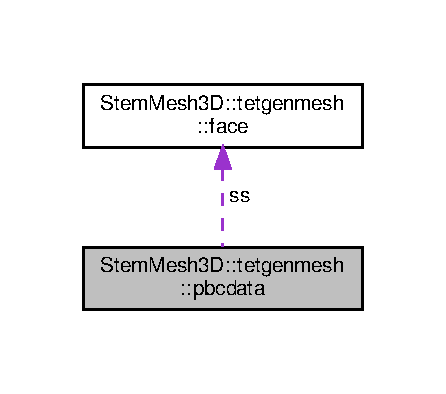
\includegraphics[width=214pt]{structStemMesh3D_1_1tetgenmesh_1_1pbcdata__coll__graph}
\end{center}
\end{figure}
\subsection*{Public Attributes}
\begin{DoxyCompactItemize}
\item 
\mbox{\Hypertarget{structStemMesh3D_1_1tetgenmesh_1_1pbcdata_a0363f11b33c98abcf3c4878c9d96d36c}\label{structStemMesh3D_1_1tetgenmesh_1_1pbcdata_a0363f11b33c98abcf3c4878c9d96d36c}} 
int {\bfseries fmark} \mbox{[}2\mbox{]}
\item 
\mbox{\Hypertarget{structStemMesh3D_1_1tetgenmesh_1_1pbcdata_af4efd5f8da71f48428db0a473be400db}\label{structStemMesh3D_1_1tetgenmesh_1_1pbcdata_af4efd5f8da71f48428db0a473be400db}} 
int {\bfseries segid} \mbox{[}2\mbox{]}
\item 
\mbox{\Hypertarget{structStemMesh3D_1_1tetgenmesh_1_1pbcdata_ae58295e2a54c79937ed906410695dec9}\label{structStemMesh3D_1_1tetgenmesh_1_1pbcdata_ae58295e2a54c79937ed906410695dec9}} 
\hyperlink{classStemMesh3D_1_1tetgenmesh_1_1face}{face} {\bfseries ss} \mbox{[}2\mbox{]}
\item 
\mbox{\Hypertarget{structStemMesh3D_1_1tetgenmesh_1_1pbcdata_a8f4a26ee38db65cbf87da7add136e008}\label{structStemMesh3D_1_1tetgenmesh_1_1pbcdata_a8f4a26ee38db65cbf87da7add136e008}} 
R\+E\+AL {\bfseries transmat} \mbox{[}2\mbox{]}\mbox{[}4\mbox{]}\mbox{[}4\mbox{]}
\end{DoxyCompactItemize}


The documentation for this struct was generated from the following file\+:\begin{DoxyCompactItemize}
\item 
src/\+Mesh/\+Stem\+Mesh/tetgen.\+h\end{DoxyCompactItemize}

\hypertarget{structStemMesh3D_1_1tetgenio_1_1pbcgroup}{}\section{Stem\+Mesh3D\+:\+:tetgenio\+:\+:pbcgroup Struct Reference}
\label{structStemMesh3D_1_1tetgenio_1_1pbcgroup}\index{Stem\+Mesh3\+D\+::tetgenio\+::pbcgroup@{Stem\+Mesh3\+D\+::tetgenio\+::pbcgroup}}
\subsection*{Public Attributes}
\begin{DoxyCompactItemize}
\item 
\mbox{\Hypertarget{structStemMesh3D_1_1tetgenio_1_1pbcgroup_aef9814e8e96446f7d4c5102ae2b1192b}\label{structStemMesh3D_1_1tetgenio_1_1pbcgroup_aef9814e8e96446f7d4c5102ae2b1192b}} 
int {\bfseries fmark1}
\item 
\mbox{\Hypertarget{structStemMesh3D_1_1tetgenio_1_1pbcgroup_ab3eb6babb3d15eba5b89065798b7b756}\label{structStemMesh3D_1_1tetgenio_1_1pbcgroup_ab3eb6babb3d15eba5b89065798b7b756}} 
int {\bfseries fmark2}
\item 
\mbox{\Hypertarget{structStemMesh3D_1_1tetgenio_1_1pbcgroup_a98b0453de3a8e630eccfd43d9fc7f505}\label{structStemMesh3D_1_1tetgenio_1_1pbcgroup_a98b0453de3a8e630eccfd43d9fc7f505}} 
R\+E\+AL {\bfseries transmat} \mbox{[}4\mbox{]}\mbox{[}4\mbox{]}
\item 
\mbox{\Hypertarget{structStemMesh3D_1_1tetgenio_1_1pbcgroup_a2912d61a7ff4905253af1510e75700d8}\label{structStemMesh3D_1_1tetgenio_1_1pbcgroup_a2912d61a7ff4905253af1510e75700d8}} 
int {\bfseries numberofpointpairs}
\item 
\mbox{\Hypertarget{structStemMesh3D_1_1tetgenio_1_1pbcgroup_ad6ece5d0e2db6b0c38328ee72b0b419c}\label{structStemMesh3D_1_1tetgenio_1_1pbcgroup_ad6ece5d0e2db6b0c38328ee72b0b419c}} 
int $\ast$ {\bfseries pointpairlist}
\end{DoxyCompactItemize}


The documentation for this struct was generated from the following file\+:\begin{DoxyCompactItemize}
\item 
src/\+Mesh/\+Stem\+Mesh/tetgen.\+h\end{DoxyCompactItemize}

\hypertarget{structStemMesh3D_1_1tetgenio_1_1polygon}{}\doxysection{Stem\+Mesh3D\+::tetgenio\+::polygon Struct Reference}
\label{structStemMesh3D_1_1tetgenio_1_1polygon}\index{StemMesh3D::tetgenio::polygon@{StemMesh3D::tetgenio::polygon}}
\doxysubsection*{Public Attributes}
\begin{DoxyCompactItemize}
\item 
\mbox{\Hypertarget{structStemMesh3D_1_1tetgenio_1_1polygon_a7a9745e3196d1e72a98e30434a6458a4}\label{structStemMesh3D_1_1tetgenio_1_1polygon_a7a9745e3196d1e72a98e30434a6458a4}} 
int $\ast$ {\bfseries vertexlist}
\item 
\mbox{\Hypertarget{structStemMesh3D_1_1tetgenio_1_1polygon_a1b49dd248dd959716f6d962d5745328f}\label{structStemMesh3D_1_1tetgenio_1_1polygon_a1b49dd248dd959716f6d962d5745328f}} 
int {\bfseries numberofvertices}
\end{DoxyCompactItemize}


The documentation for this struct was generated from the following file\+:\begin{DoxyCompactItemize}
\item 
src/\+Mesh/\+Stem\+Mesh/tetgen.\+h\end{DoxyCompactItemize}

\hypertarget{structHArDCore3D_1_1QuadratureNode}{}\section{H\+Ar\+D\+Core3D\+:\+:Quadrature\+Node Struct Reference}
\label{structHArDCore3D_1_1QuadratureNode}\index{H\+Ar\+D\+Core3\+D\+::\+Quadrature\+Node@{H\+Ar\+D\+Core3\+D\+::\+Quadrature\+Node}}


Description of one node and one weight from a quadrature rule.  




{\ttfamily \#include $<$quadraturerule.\+hpp$>$}

\subsection*{Public Member Functions}
\begin{DoxyCompactItemize}
\item 
{\bfseries Quadrature\+Node} (double x, double y, double z, double w)
\item 
Eigen\+::\+Vector3d \hyperlink{group__Quadratures_gac0d94c3725c0502056333f314fb48fc9}{vector} () const
\begin{DoxyCompactList}\small\item\em Returns the quadrature point as an Eigen vector. \end{DoxyCompactList}\end{DoxyCompactItemize}
\subsection*{Public Attributes}
\begin{DoxyCompactItemize}
\item 
double {\bfseries x}
\item 
double {\bfseries y}
\item 
double {\bfseries z}
\item 
double {\bfseries w}
\end{DoxyCompactItemize}


\subsection{Detailed Description}
Description of one node and one weight from a quadrature rule. 

The documentation for this struct was generated from the following file\+:\begin{DoxyCompactItemize}
\item 
src/\+Quadrature/quadraturerule.\+hpp\end{DoxyCompactItemize}

\hypertarget{classStemMesh3D_1_1QuadRegion}{}\doxysection{Stem\+Mesh3D\+::Quad\+Region Class Reference}
\label{classStemMesh3D_1_1QuadRegion}\index{StemMesh3D::QuadRegion@{StemMesh3D::QuadRegion}}
\doxysubsection*{Public Member Functions}
\begin{DoxyCompactItemize}
\item 
\mbox{\Hypertarget{classStemMesh3D_1_1QuadRegion_a561cd08cd2430d205ce0dddefc967f0f}\label{classStemMesh3D_1_1QuadRegion_a561cd08cd2430d205ce0dddefc967f0f}} 
{\bfseries Quad\+Region} (\mbox{\hyperlink{classStemMesh3D_1_1mesh__3Dv}{mesh\+\_\+3\+Dv}} \&\+\_\+mesh, int \+\_\+rule=0)
\item 
\mbox{\Hypertarget{classStemMesh3D_1_1QuadRegion_a865123e616e3661727dbcfd05f249c64}\label{classStemMesh3D_1_1QuadRegion_a865123e616e3661727dbcfd05f249c64}} 
void {\bfseries setup} (int \+\_\+iR)
\item 
\mbox{\Hypertarget{classStemMesh3D_1_1QuadRegion_a4d7ff91015551a159f3a06458d4f915d}\label{classStemMesh3D_1_1QuadRegion_a4d7ff91015551a159f3a06458d4f915d}} 
void {\bfseries setup\+\_\+tetgenio} ()
\item 
\mbox{\Hypertarget{classStemMesh3D_1_1QuadRegion_aa669969c5ab1f32b79c170bbfa4fff0e}\label{classStemMesh3D_1_1QuadRegion_aa669969c5ab1f32b79c170bbfa4fff0e}} 
void {\bfseries region\+\_\+intg\+\_\+values} (double \&vol\+\_\+R, double \&xR, double \&yR, double \&zR)
\item 
\mbox{\Hypertarget{classStemMesh3D_1_1QuadRegion_ab93715c2cec77bb4bbb66e33582c58a2}\label{classStemMesh3D_1_1QuadRegion_ab93715c2cec77bb4bbb66e33582c58a2}} 
double {\bfseries region\+\_\+intg} (double func(double, double, double))
\item 
\mbox{\Hypertarget{classStemMesh3D_1_1QuadRegion_a00bb9d3b1281205987b9c7fe313adfd1}\label{classStemMesh3D_1_1QuadRegion_a00bb9d3b1281205987b9c7fe313adfd1}} 
{\footnotesize template$<$class F\+U\+N\+C\+T\+I\+O\+N\+\_\+\+O\+B\+J\+E\+CT $>$ }\\double {\bfseries region\+\_\+integral} (F\+U\+N\+C\+T\+I\+O\+N\+\_\+\+O\+B\+J\+E\+CT \&func\+\_\+obj)
\item 
\mbox{\Hypertarget{classStemMesh3D_1_1QuadRegion_a8a765eb6c1524bb2d7cb40e8397e42bc}\label{classStemMesh3D_1_1QuadRegion_a8a765eb6c1524bb2d7cb40e8397e42bc}} 
{\footnotesize template$<$class F\+U\+N\+C\+T\+I\+O\+N\+\_\+\+O\+B\+J\+E\+CT $>$ }\\double {\bfseries region\+\_\+integral} (int i, F\+U\+N\+C\+T\+I\+O\+N\+\_\+\+O\+B\+J\+E\+CT \&func\+\_\+obj)
\item 
\mbox{\Hypertarget{classStemMesh3D_1_1QuadRegion_ad9694c8d6c595fdbe0963a04e727bb6e}\label{classStemMesh3D_1_1QuadRegion_ad9694c8d6c595fdbe0963a04e727bb6e}} 
int {\bfseries n\+\_\+tetra} ()
\item 
\mbox{\Hypertarget{classStemMesh3D_1_1QuadRegion_a9c1a9ba6f359ba0d37939e55bd38f5c3}\label{classStemMesh3D_1_1QuadRegion_a9c1a9ba6f359ba0d37939e55bd38f5c3}} 
int {\bfseries get\+\_\+nq} ()
\item 
\mbox{\Hypertarget{classStemMesh3D_1_1QuadRegion_aa69916e213e1d385d57bfa98eeaa101c}\label{classStemMesh3D_1_1QuadRegion_aa69916e213e1d385d57bfa98eeaa101c}} 
void {\bfseries set\+\_\+quadrule} (int iT)
\item 
\mbox{\Hypertarget{classStemMesh3D_1_1QuadRegion_a42a9671805580d53fd2ca5ecfb763e2d}\label{classStemMesh3D_1_1QuadRegion_a42a9671805580d53fd2ca5ecfb763e2d}} 
void {\bfseries get\+\_\+quadrule} (int iq, double \&xq, double \&yq, double \&zq, double \&wq)
\end{DoxyCompactItemize}


The documentation for this class was generated from the following file\+:\begin{DoxyCompactItemize}
\item 
src/\+Mesh/\+Stem\+Mesh/quad\+\_\+regn.\+hh\end{DoxyCompactItemize}

\hypertarget{classHArDCore3D_1_1QuadRuleEdge}{}\section{H\+Ar\+D\+Core3D\+:\+:Quad\+Rule\+Edge Class Reference}
\label{classHArDCore3D_1_1QuadRuleEdge}\index{H\+Ar\+D\+Core3\+D\+::\+Quad\+Rule\+Edge@{H\+Ar\+D\+Core3\+D\+::\+Quad\+Rule\+Edge}}
\subsection*{Public Member Functions}
\begin{DoxyCompactItemize}
\item 
\mbox{\Hypertarget{classHArDCore3D_1_1QuadRuleEdge_abb254b22a706f3781b2b8a7b3fafa288}\label{classHArDCore3D_1_1QuadRuleEdge_abb254b22a706f3781b2b8a7b3fafa288}} 
{\bfseries Quad\+Rule\+Edge} (size\+\_\+t doe, bool warn)
\item 
\mbox{\Hypertarget{classHArDCore3D_1_1QuadRuleEdge_af245dd9ab99a15742641d81f5508041a}\label{classHArDCore3D_1_1QuadRuleEdge_af245dd9ab99a15742641d81f5508041a}} 
size\+\_\+t {\bfseries nq} ()
\item 
\mbox{\Hypertarget{classHArDCore3D_1_1QuadRuleEdge_a1b03cf6a6800470a027f570d44338a1f}\label{classHArDCore3D_1_1QuadRuleEdge_a1b03cf6a6800470a027f570d44338a1f}} 
double {\bfseries xq} (size\+\_\+t i)
\item 
\mbox{\Hypertarget{classHArDCore3D_1_1QuadRuleEdge_ac272eee335dc95a46787e1a054b38cb7}\label{classHArDCore3D_1_1QuadRuleEdge_ac272eee335dc95a46787e1a054b38cb7}} 
double {\bfseries yq} (size\+\_\+t i)
\item 
\mbox{\Hypertarget{classHArDCore3D_1_1QuadRuleEdge_a2172f93f9d6679d07b37ac76f59c5282}\label{classHArDCore3D_1_1QuadRuleEdge_a2172f93f9d6679d07b37ac76f59c5282}} 
double {\bfseries zq} (size\+\_\+t i)
\item 
\mbox{\Hypertarget{classHArDCore3D_1_1QuadRuleEdge_a3fc5a686c8018dbea8ec3a120ad6d9bc}\label{classHArDCore3D_1_1QuadRuleEdge_a3fc5a686c8018dbea8ec3a120ad6d9bc}} 
double {\bfseries wq} (size\+\_\+t i)
\item 
\mbox{\Hypertarget{classHArDCore3D_1_1QuadRuleEdge_a362bb5fef8a2d98073605945c89aadf9}\label{classHArDCore3D_1_1QuadRuleEdge_a362bb5fef8a2d98073605945c89aadf9}} 
void {\bfseries setup} (double xV\mbox{[}$\,$\mbox{]}, double yV\mbox{[}$\,$\mbox{]}, double zV\mbox{[}$\,$\mbox{]})
\end{DoxyCompactItemize}


The documentation for this class was generated from the following files\+:\begin{DoxyCompactItemize}
\item 
src/\+Quadrature/quad1d.\+hpp\item 
src/\+Quadrature/quad1d.\+cpp\end{DoxyCompactItemize}

\hypertarget{classHArDCore3D_1_1QuadRuleTetra}{}\section{H\+Ar\+D\+Core3D\+:\+:Quad\+Rule\+Tetra Class Reference}
\label{classHArDCore3D_1_1QuadRuleTetra}\index{H\+Ar\+D\+Core3\+D\+::\+Quad\+Rule\+Tetra@{H\+Ar\+D\+Core3\+D\+::\+Quad\+Rule\+Tetra}}
\subsection*{Public Member Functions}
\begin{DoxyCompactItemize}
\item 
\hyperlink{classHArDCore3D_1_1QuadRuleTetra_aa9690d2663c19c67d52b3cd176afa4b9}{Quad\+Rule\+Tetra} (size\+\_\+t doe, bool warn)
\begin{DoxyCompactList}\small\item\em Create a quadrature rule with at least the given degree of exactness (if available). \end{DoxyCompactList}\item 
\mbox{\Hypertarget{classHArDCore3D_1_1QuadRuleTetra_a7a95e2c4005af1f7dc71da864d1e79e3}\label{classHArDCore3D_1_1QuadRuleTetra_a7a95e2c4005af1f7dc71da864d1e79e3}} 
{\bfseries Quad\+Rule\+Tetra} (size\+\_\+t \+\_\+rule=0)
\item 
size\+\_\+t {\bfseries nq} () const
\item 
double {\bfseries xq} (int iq) const
\item 
double {\bfseries yq} (int iq) const
\item 
double {\bfseries zq} (int iq) const
\item 
double {\bfseries wq} (int iq) const
\item 
\mbox{\Hypertarget{classHArDCore3D_1_1QuadRuleTetra_aa38c3a679cd52d2157653acb3013984b}\label{classHArDCore3D_1_1QuadRuleTetra_aa38c3a679cd52d2157653acb3013984b}} 
void {\bfseries setup} (double(\&\+\_\+xV)\mbox{[}4\mbox{]}, double(\&\+\_\+yV)\mbox{[}4\mbox{]}, double(\&\+\_\+zV)\mbox{[}4\mbox{]})
\item 
\mbox{\Hypertarget{classHArDCore3D_1_1QuadRuleTetra_a0b28a2844825ec7d4f26678ddbb119f4}\label{classHArDCore3D_1_1QuadRuleTetra_a0b28a2844825ec7d4f26678ddbb119f4}} 
void {\bfseries get\+\_\+quadrule} (int iq, double \&\+\_\+xq, double \&\+\_\+yq, double \&\+\_\+zq, double \&\+\_\+wq) const
\end{DoxyCompactItemize}
\subsection*{Protected Member Functions}
\begin{DoxyCompactItemize}
\item 
\mbox{\Hypertarget{classHArDCore3D_1_1QuadRuleTetra_aea9fa6144096012c2ea7f5b220493ef8}\label{classHArDCore3D_1_1QuadRuleTetra_aea9fa6144096012c2ea7f5b220493ef8}} 
void {\bfseries init} ()
\item 
size\+\_\+t \hyperlink{classHArDCore3D_1_1QuadRuleTetra_aaa2822c1275680abfc0ee93690b1a9b7}{required\+\_\+rule} (size\+\_\+t doe) const
\begin{DoxyCompactList}\small\item\em Compute the minimum rule required to achieve the desired degree of exactness. \end{DoxyCompactList}\end{DoxyCompactItemize}
\subsection*{Protected Attributes}
\begin{DoxyCompactItemize}
\item 
\mbox{\Hypertarget{classHArDCore3D_1_1QuadRuleTetra_a2c9c89e52d8048abbc8f57b394d4b384}\label{classHArDCore3D_1_1QuadRuleTetra_a2c9c89e52d8048abbc8f57b394d4b384}} 
const size\+\_\+t {\bfseries rule}
\item 
\mbox{\Hypertarget{classHArDCore3D_1_1QuadRuleTetra_acb524e378f7d076b353f8957f5861af8}\label{classHArDCore3D_1_1QuadRuleTetra_acb524e378f7d076b353f8957f5861af8}} 
const size\+\_\+t {\bfseries nqn}
\item 
\mbox{\Hypertarget{classHArDCore3D_1_1QuadRuleTetra_a89340eddcfc957b975316e4e70122880}\label{classHArDCore3D_1_1QuadRuleTetra_a89340eddcfc957b975316e4e70122880}} 
double {\bfseries vol\+\_\+T}
\item 
\mbox{\Hypertarget{classHArDCore3D_1_1QuadRuleTetra_a6a4a14f830d50341f73ebcaefcf6d2a4}\label{classHArDCore3D_1_1QuadRuleTetra_a6a4a14f830d50341f73ebcaefcf6d2a4}} 
std\+::vector$<$ double $>$ {\bfseries xV}
\item 
\mbox{\Hypertarget{classHArDCore3D_1_1QuadRuleTetra_af862c47f073d3ed8f7b46b2aec2f02bf}\label{classHArDCore3D_1_1QuadRuleTetra_af862c47f073d3ed8f7b46b2aec2f02bf}} 
std\+::vector$<$ double $>$ {\bfseries yV}
\item 
\mbox{\Hypertarget{classHArDCore3D_1_1QuadRuleTetra_a9a14973f22d456a9b9f62104e27ee15c}\label{classHArDCore3D_1_1QuadRuleTetra_a9a14973f22d456a9b9f62104e27ee15c}} 
std\+::vector$<$ double $>$ {\bfseries zV}
\item 
\mbox{\Hypertarget{classHArDCore3D_1_1QuadRuleTetra_acf9bd31067eedbde378811923330002e}\label{classHArDCore3D_1_1QuadRuleTetra_acf9bd31067eedbde378811923330002e}} 
std\+::vector$<$ double $>$ {\bfseries cq0}
\item 
\mbox{\Hypertarget{classHArDCore3D_1_1QuadRuleTetra_a4ac6c16943d4a2f8670cbf7ee4a975cf}\label{classHArDCore3D_1_1QuadRuleTetra_a4ac6c16943d4a2f8670cbf7ee4a975cf}} 
std\+::vector$<$ double $>$ {\bfseries cq1}
\item 
\mbox{\Hypertarget{classHArDCore3D_1_1QuadRuleTetra_a05ec9999eee3a2f2abfd89d556c07bcd}\label{classHArDCore3D_1_1QuadRuleTetra_a05ec9999eee3a2f2abfd89d556c07bcd}} 
std\+::vector$<$ double $>$ {\bfseries cq2}
\item 
\mbox{\Hypertarget{classHArDCore3D_1_1QuadRuleTetra_a7b7435493531e382c3a697b704f8c3d2}\label{classHArDCore3D_1_1QuadRuleTetra_a7b7435493531e382c3a697b704f8c3d2}} 
std\+::vector$<$ double $>$ {\bfseries cq3}
\item 
\mbox{\Hypertarget{classHArDCore3D_1_1QuadRuleTetra_a48814d986ec321ceb67e49d04e46562d}\label{classHArDCore3D_1_1QuadRuleTetra_a48814d986ec321ceb67e49d04e46562d}} 
std\+::vector$<$ double $>$ {\bfseries cwq}
\end{DoxyCompactItemize}
\subsection*{Static Protected Attributes}
\begin{DoxyCompactItemize}
\item 
\mbox{\Hypertarget{classHArDCore3D_1_1QuadRuleTetra_ab26709dc12bd459dcabe7c64a6976509}\label{classHArDCore3D_1_1QuadRuleTetra_ab26709dc12bd459dcabe7c64a6976509}} 
static constexpr size\+\_\+t {\bfseries max\+\_\+doe} = 14
\item 
\mbox{\Hypertarget{classHArDCore3D_1_1QuadRuleTetra_ab0c5c48d113c568e34353ccb1a9c5321}\label{classHArDCore3D_1_1QuadRuleTetra_ab0c5c48d113c568e34353ccb1a9c5321}} 
static constexpr size\+\_\+t {\bfseries num\+\_\+rules} = 15
\end{DoxyCompactItemize}


\subsection{Constructor \& Destructor Documentation}
\mbox{\Hypertarget{classHArDCore3D_1_1QuadRuleTetra_aa9690d2663c19c67d52b3cd176afa4b9}\label{classHArDCore3D_1_1QuadRuleTetra_aa9690d2663c19c67d52b3cd176afa4b9}} 
\index{H\+Ar\+D\+Core3\+D\+::\+Quad\+Rule\+Tetra@{H\+Ar\+D\+Core3\+D\+::\+Quad\+Rule\+Tetra}!Quad\+Rule\+Tetra@{Quad\+Rule\+Tetra}}
\index{Quad\+Rule\+Tetra@{Quad\+Rule\+Tetra}!H\+Ar\+D\+Core3\+D\+::\+Quad\+Rule\+Tetra@{H\+Ar\+D\+Core3\+D\+::\+Quad\+Rule\+Tetra}}
\subsubsection{\texorpdfstring{Quad\+Rule\+Tetra()}{QuadRuleTetra()}}
{\footnotesize\ttfamily Quad\+Rule\+Tetra\+::\+Quad\+Rule\+Tetra (\begin{DoxyParamCaption}\item[{size\+\_\+t}]{doe,  }\item[{bool}]{warn }\end{DoxyParamCaption})}



Create a quadrature rule with at least the given degree of exactness (if available). 

The smallest such quadrature rule will be chosen. If none are available, the highest degree available will be used. 

\subsection{Member Function Documentation}
\mbox{\Hypertarget{classHArDCore3D_1_1QuadRuleTetra_aaa2822c1275680abfc0ee93690b1a9b7}\label{classHArDCore3D_1_1QuadRuleTetra_aaa2822c1275680abfc0ee93690b1a9b7}} 
\index{H\+Ar\+D\+Core3\+D\+::\+Quad\+Rule\+Tetra@{H\+Ar\+D\+Core3\+D\+::\+Quad\+Rule\+Tetra}!required\+\_\+rule@{required\+\_\+rule}}
\index{required\+\_\+rule@{required\+\_\+rule}!H\+Ar\+D\+Core3\+D\+::\+Quad\+Rule\+Tetra@{H\+Ar\+D\+Core3\+D\+::\+Quad\+Rule\+Tetra}}
\subsubsection{\texorpdfstring{required\+\_\+rule()}{required\_rule()}}
{\footnotesize\ttfamily size\+\_\+t Quad\+Rule\+Tetra\+::required\+\_\+rule (\begin{DoxyParamCaption}\item[{size\+\_\+t}]{doe }\end{DoxyParamCaption}) const\hspace{0.3cm}{\ttfamily [protected]}}



Compute the minimum rule required to achieve the desired degree of exactness. 

If no such rule exists, returns the highest rule. 

The documentation for this class was generated from the following files\+:\begin{DoxyCompactItemize}
\item 
src/\+Quadrature/quad3d.\+hpp\item 
src/\+Quadrature/quad3d.\+cpp\end{DoxyCompactItemize}

\hypertarget{classHArDCore3D_1_1QuadRuleTriangle}{}\section{H\+Ar\+D\+Core3D\+:\+:Quad\+Rule\+Triangle Class Reference}
\label{classHArDCore3D_1_1QuadRuleTriangle}\index{H\+Ar\+D\+Core3\+D\+::\+Quad\+Rule\+Triangle@{H\+Ar\+D\+Core3\+D\+::\+Quad\+Rule\+Triangle}}
\subsection*{Public Member Functions}
\begin{DoxyCompactItemize}
\item 
\hyperlink{group__Quadratures_ga0d95447bb72cfc1b19cd2ea192ff6695}{Quad\+Rule\+Triangle} (size\+\_\+t \+\_\+doe, bool warn)
\begin{DoxyCompactList}\small\item\em Default constructor. \end{DoxyCompactList}\item 
double {\bfseries xq} (size\+\_\+t i)
\item 
double {\bfseries yq} (size\+\_\+t i)
\item 
double {\bfseries zq} (size\+\_\+t i)
\item 
double {\bfseries wq} (size\+\_\+t i)
\item 
size\+\_\+t {\bfseries nq} ()
\item 
void {\bfseries setup} (double xV\mbox{[}$\,$\mbox{]}, double yV\mbox{[}$\,$\mbox{]}, double zV\mbox{[}$\,$\mbox{]})
\end{DoxyCompactItemize}
\subsection*{Protected Member Functions}
\begin{DoxyCompactItemize}
\item 
double {\bfseries area} (double xV\mbox{[}$\,$\mbox{]}, double yV\mbox{[}$\,$\mbox{]}, double zV\mbox{[}$\,$\mbox{]}) const
\end{DoxyCompactItemize}
\subsection*{Protected Attributes}
\begin{DoxyCompactItemize}
\item 
size\+\_\+t {\bfseries \+\_\+npts}
\item 
double $\ast$ {\bfseries qsx}
\item 
double $\ast$ {\bfseries qsy}
\item 
double $\ast$ {\bfseries qsz}
\item 
double $\ast$ {\bfseries qswg}
\item 
double $\ast$ {\bfseries \+\_\+xy}
\item 
double $\ast$ {\bfseries \+\_\+w}
\end{DoxyCompactItemize}


The documentation for this class was generated from the following files\+:\begin{DoxyCompactItemize}
\item 
src/\+Quadrature/quad3d\+\_\+face.\+hpp\item 
src/\+Quadrature/quad3d\+\_\+face.\+cpp\end{DoxyCompactItemize}

\hypertarget{classStemMesh3D_1_1tetgenmesh_1_1queue}{}\doxysection{Stem\+Mesh3D\+::tetgenmesh\+::queue Class Reference}
\label{classStemMesh3D_1_1tetgenmesh_1_1queue}\index{StemMesh3D::tetgenmesh::queue@{StemMesh3D::tetgenmesh::queue}}


Inheritance diagram for Stem\+Mesh3D\+::tetgenmesh\+::queue\+:\nopagebreak
\begin{figure}[H]
\begin{center}
\leavevmode
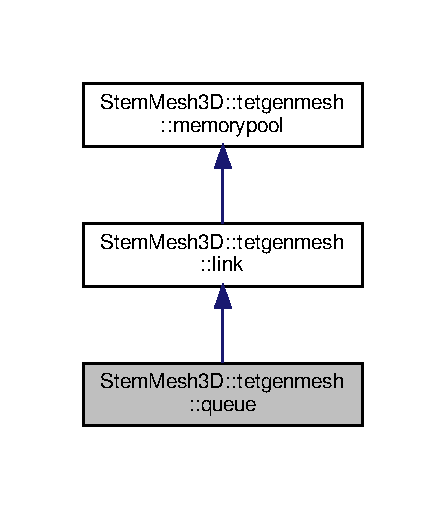
\includegraphics[width=214pt]{classStemMesh3D_1_1tetgenmesh_1_1queue__inherit__graph}
\end{center}
\end{figure}


Collaboration diagram for Stem\+Mesh3D\+::tetgenmesh\+::queue\+:\nopagebreak
\begin{figure}[H]
\begin{center}
\leavevmode
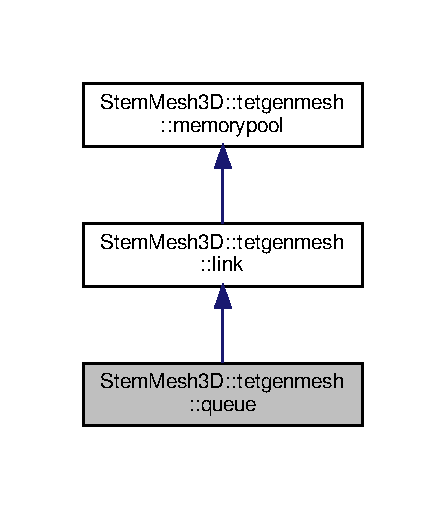
\includegraphics[width=214pt]{classStemMesh3D_1_1tetgenmesh_1_1queue__coll__graph}
\end{center}
\end{figure}
\doxysubsection*{Public Member Functions}
\begin{DoxyCompactItemize}
\item 
\mbox{\Hypertarget{classStemMesh3D_1_1tetgenmesh_1_1queue_ab65ecff2fd73d3f7fd223dceed1a2946}\label{classStemMesh3D_1_1tetgenmesh_1_1queue_ab65ecff2fd73d3f7fd223dceed1a2946}} 
{\bfseries queue} (int bytes, int count=256)
\item 
\mbox{\Hypertarget{classStemMesh3D_1_1tetgenmesh_1_1queue_a356323fdbf2433aac8a79cfc8621699f}\label{classStemMesh3D_1_1tetgenmesh_1_1queue_a356323fdbf2433aac8a79cfc8621699f}} 
{\bfseries queue} (char $\ast$str, int count=256)
\item 
\mbox{\Hypertarget{classStemMesh3D_1_1tetgenmesh_1_1queue_af35c5ed15086504182e24417f4af759b}\label{classStemMesh3D_1_1tetgenmesh_1_1queue_af35c5ed15086504182e24417f4af759b}} 
int {\bfseries empty} ()
\item 
\mbox{\Hypertarget{classStemMesh3D_1_1tetgenmesh_1_1queue_a68f8c01a4679af06ea4f00d37f6ee4ec}\label{classStemMesh3D_1_1tetgenmesh_1_1queue_a68f8c01a4679af06ea4f00d37f6ee4ec}} 
void $\ast$ {\bfseries push} (void $\ast$newitem)
\item 
\mbox{\Hypertarget{classStemMesh3D_1_1tetgenmesh_1_1queue_a5e1e1f963ffcf2cede9657c350daeec0}\label{classStemMesh3D_1_1tetgenmesh_1_1queue_a5e1e1f963ffcf2cede9657c350daeec0}} 
void $\ast$ {\bfseries bot} ()
\item 
\mbox{\Hypertarget{classStemMesh3D_1_1tetgenmesh_1_1queue_a7007cb39ed4937e670dbc0512842ee13}\label{classStemMesh3D_1_1tetgenmesh_1_1queue_a7007cb39ed4937e670dbc0512842ee13}} 
void $\ast$ {\bfseries pop} ()
\end{DoxyCompactItemize}
\doxysubsection*{Additional Inherited Members}


The documentation for this class was generated from the following file\+:\begin{DoxyCompactItemize}
\item 
src/\+Mesh/\+Stem\+Mesh/tetgen.\+h\end{DoxyCompactItemize}

\hypertarget{classHArDCore3D_1_1RestrictedBasis}{}\doxysection{H\+Ar\+D\+Core3D\+::Restricted\+Basis$<$ Basis\+Type $>$ Class Template Reference}
\label{classHArDCore3D_1_1RestrictedBasis}\index{HArDCore3D::RestrictedBasis$<$ BasisType $>$@{HArDCore3D::RestrictedBasis$<$ BasisType $>$}}


Generate a basis restricted to the first \char`\"{}dimension\char`\"{} functions.  




{\ttfamily \#include $<$basis.\+hpp$>$}

\doxysubsection*{Public Types}
\begin{DoxyCompactItemize}
\item 
typedef Basis\+Type\+::\+Function\+Value {\bfseries Function\+Value}
\item 
typedef Basis\+Type\+::\+Gradient\+Value {\bfseries Gradient\+Value}
\item 
typedef Vector\+Rd {\bfseries Curl\+Value}
\item 
typedef double {\bfseries Divergence\+Value}
\item 
typedef Basis\+Type\+::\+Geometric\+Support {\bfseries Geometric\+Support}
\end{DoxyCompactItemize}
\doxysubsection*{Public Member Functions}
\begin{DoxyCompactItemize}
\item 
\mbox{\hyperlink{group__Common_gac9623c0deb32ee33cb10de45f4f75702}{Restricted\+Basis}} (const Basis\+Type \&basis, const size\+\_\+t \&\mbox{\hyperlink{group__Common_gaf281956665b32bc8613043e4f303182e}{dimension}})
\begin{DoxyCompactList}\small\item\em Constructor. \end{DoxyCompactList}\item 
size\+\_\+t \mbox{\hyperlink{group__Common_gaf281956665b32bc8613043e4f303182e}{dimension}} () const
\begin{DoxyCompactList}\small\item\em Return the dimension of the basis. \end{DoxyCompactList}\item 
const Basis\+Type \& \mbox{\hyperlink{group__Common_ga69735cd402a3190ebd982269f4cb1582}{ancestor}} () const
\begin{DoxyCompactList}\small\item\em Return the underlying complete basis. \end{DoxyCompactList}\item 
Function\+Value \mbox{\hyperlink{group__Common_gacb26aa08f1f3d62deb174e82dc9c2046}{function}} (size\+\_\+t i, const Vector\+Rd \&x) const
\begin{DoxyCompactList}\small\item\em Evaluate the i-\/th basis function at point x. \end{DoxyCompactList}\item 
Gradient\+Value \mbox{\hyperlink{group__Common_gae191627737010694521dc5aae42744cd}{gradient}} (size\+\_\+t i, const Vector\+Rd \&x) const
\begin{DoxyCompactList}\small\item\em Evaluate the gradient of the i-\/th basis function at point x. \end{DoxyCompactList}\item 
Curl\+Value \mbox{\hyperlink{group__Common_ga6886d8130d38f8e0cdeac3c53fe9e177}{curl}} (size\+\_\+t i, const Vector\+Rd \&x) const
\begin{DoxyCompactList}\small\item\em Evaluate the curl of the i-\/th basis function at point x. \end{DoxyCompactList}\item 
Divergence\+Value \mbox{\hyperlink{group__Common_ga06c5ecd7cb9ce4c52891c355a5dc2108}{divergence}} (size\+\_\+t i, const Vector\+Rd \&x) const
\begin{DoxyCompactList}\small\item\em Evaluate the divergence of the i-\/th basis function at point x. \end{DoxyCompactList}\end{DoxyCompactItemize}
\doxysubsection*{Static Public Attributes}
\begin{DoxyCompactItemize}
\item 
static const Tensor\+RankE {\bfseries tensor\+Rank} = Basis\+Type\+::tensor\+Rank
\item 
static const bool {\bfseries has\+Function} = Basis\+Type\+::has\+Function
\item 
static const bool {\bfseries has\+Gradient} = Basis\+Type\+::has\+Gradient
\item 
static const bool {\bfseries has\+Curl} = Basis\+Type\+::has\+Curl
\item 
static const bool {\bfseries has\+Divergence} = Basis\+Type\+::has\+Divergence
\end{DoxyCompactItemize}


\doxysubsection{Detailed Description}
\subsubsection*{template$<$typename Basis\+Type$>$\newline
class H\+Ar\+D\+Core3\+D\+::\+Restricted\+Basis$<$ Basis\+Type $>$}

Generate a basis restricted to the first \char`\"{}dimension\char`\"{} functions. 

This can be useful, e.\+g., to form bases of subspaces of a given space from a hierarchical basis of the latter 

The documentation for this class was generated from the following file\+:\begin{DoxyCompactItemize}
\item 
src/\+Common/basis.\+hpp\end{DoxyCompactItemize}

\hypertarget{classHArDCore3D_1_1ShiftedBasis}{}\doxysection{H\+Ar\+D\+Core3D\+::Shifted\+Basis$<$ Basis\+Type $>$ Class Template Reference}
\label{classHArDCore3D_1_1ShiftedBasis}\index{HArDCore3D::ShiftedBasis$<$ BasisType $>$@{HArDCore3D::ShiftedBasis$<$ BasisType $>$}}


{\ttfamily \#include $<$basis.\+hpp$>$}

\doxysubsection*{Public Types}
\begin{DoxyCompactItemize}
\item 
typedef Basis\+Type\+::\+Function\+Value {\bfseries Function\+Value}
\item 
typedef Basis\+Type\+::\+Gradient\+Value {\bfseries Gradient\+Value}
\item 
typedef Vector\+Rd {\bfseries Curl\+Value}
\item 
typedef double {\bfseries Divergence\+Value}
\item 
typedef Basis\+Type\+::\+Geometric\+Support {\bfseries Geometric\+Support}
\end{DoxyCompactItemize}
\doxysubsection*{Public Member Functions}
\begin{DoxyCompactItemize}
\item 
\mbox{\hyperlink{group__Basis_gaea075c3cb8fbdd848e30d84821f23711}{Shifted\+Basis}} (const Basis\+Type \&basis, const int shift)
\begin{DoxyCompactList}\small\item\em Constructor. \end{DoxyCompactList}\item 
size\+\_\+t \mbox{\hyperlink{group__Basis_ga0d1ffbb1cb714755de9035fcb9d5f183}{dimension}} () const
\begin{DoxyCompactList}\small\item\em Return the dimension of the basis. \end{DoxyCompactList}\item 
Function\+Value \mbox{\hyperlink{group__Basis_ga67db64c53524c17389e1928ff7288101}{function}} (size\+\_\+t i, const Vector\+Rd \&x) const
\begin{DoxyCompactList}\small\item\em Evaluate the i-\/th basis function at point x. \end{DoxyCompactList}\item 
Gradient\+Value \mbox{\hyperlink{group__Basis_ga1e825cd8aa68c4e1a1e3900e24be84f7}{gradient}} (size\+\_\+t i, const Vector\+Rd \&x) const
\begin{DoxyCompactList}\small\item\em Evaluate the gradient of the i-\/th basis function at point x. \end{DoxyCompactList}\item 
Curl\+Value \mbox{\hyperlink{group__Basis_gadca4290363039ead695cd70ca589e04d}{curl}} (size\+\_\+t i, const Vector\+Rd \&x) const
\begin{DoxyCompactList}\small\item\em Evaluate the curl of the i-\/th basis function at point x. \end{DoxyCompactList}\item 
Divergence\+Value \mbox{\hyperlink{group__Basis_ga667f2913df630001dcc7d693662af926}{divergence}} (size\+\_\+t i, const Vector\+Rd \&x) const
\begin{DoxyCompactList}\small\item\em Evaluate the divergence of the i-\/th basis function at point x. \end{DoxyCompactList}\end{DoxyCompactItemize}
\doxysubsection*{Static Public Attributes}
\begin{DoxyCompactItemize}
\item 
static const Tensor\+RankE {\bfseries tensor\+Rank} = Basis\+Type\+::tensor\+Rank
\item 
static const bool {\bfseries has\+Function} = Basis\+Type\+::has\+Function
\item 
static const bool {\bfseries has\+Gradient} = Basis\+Type\+::has\+Gradient
\item 
static const bool {\bfseries has\+Curl} = Basis\+Type\+::has\+Curl
\item 
static const bool {\bfseries has\+Divergence} = Basis\+Type\+::has\+Divergence
\end{DoxyCompactItemize}


\doxysubsection{Detailed Description}
\subsubsection*{template$<$typename Basis\+Type$>$\newline
class H\+Ar\+D\+Core3\+D\+::\+Shifted\+Basis$<$ Basis\+Type $>$}

Generate a basis where the function indices are shifted. Can be used, e.\+g., to ignore the constant function in scalar bases 

The documentation for this class was generated from the following file\+:\begin{DoxyCompactItemize}
\item 
src/\+Common/basis.\+hpp\end{DoxyCompactItemize}

\hypertarget{classHArDCore3D_1_1TangentFamily}{}\doxysection{H\+Ar\+D\+Core3D\+::Tangent\+Family$<$ Scalar\+Family\+Type $>$ Class Template Reference}
\label{classHArDCore3D_1_1TangentFamily}\index{HArDCore3D::TangentFamily$<$ ScalarFamilyType $>$@{HArDCore3D::TangentFamily$<$ ScalarFamilyType $>$}}


Vector family for polynomial functions that are tangent to a certain place (determined by the generators)  




{\ttfamily \#include $<$basis.\+hpp$>$}

\doxysubsection*{Public Types}
\begin{DoxyCompactItemize}
\item 
typedef Vector\+Rd {\bfseries Function\+Value}
\item 
typedef Eigen\+::\+Matrix$<$ double, dimspace, dimspace $>$ {\bfseries Gradient\+Value}
\item 
typedef Vector\+Rd {\bfseries Curl\+Value}
\item 
typedef double {\bfseries Divergence\+Value}
\item 
typedef \mbox{\hyperlink{classHArDCore3D_1_1Face}{Face}} {\bfseries Geometric\+Support}
\end{DoxyCompactItemize}
\doxysubsection*{Public Member Functions}
\begin{DoxyCompactItemize}
\item 
\mbox{\hyperlink{group__Common_gadf75daa62a416097ab9c2ec133dd3553}{Tangent\+Family}} (const Scalar\+Family\+Type \&scalar\+\_\+family, const Eigen\+::\+Matrix$<$ double, 2, dimspace $>$ \&generators)
\begin{DoxyCompactList}\small\item\em Constructor. \end{DoxyCompactList}\item 
size\+\_\+t \mbox{\hyperlink{group__Common_ga0c8e2840a23a7f9703ca75a9504b2423}{dimension}} () const
\begin{DoxyCompactList}\small\item\em Return the dimension of the family. \end{DoxyCompactList}\item 
Function\+Value \mbox{\hyperlink{group__Common_ga77132c1ffe753b76526c730aac3eec1e}{function}} (size\+\_\+t i, const Vector\+Rd \&x) const
\begin{DoxyCompactList}\small\item\em Evaluate the i-\/th basis function at point x. \end{DoxyCompactList}\item 
Divergence\+Value \mbox{\hyperlink{group__Common_ga7b41039db007f6410867f68954b69ede}{divergence}} (size\+\_\+t i, const Vector\+Rd \&x) const
\begin{DoxyCompactList}\small\item\em Evaluate the divergence of the i-\/th basis function at point x. \end{DoxyCompactList}\end{DoxyCompactItemize}
\doxysubsection*{Static Public Attributes}
\begin{DoxyCompactItemize}
\item 
static const Tensor\+RankE {\bfseries tensor\+Rank} = Vector
\item 
static const bool {\bfseries has\+Function} = true
\item 
static const bool {\bfseries has\+Gradient} = false
\item 
static const bool {\bfseries has\+Curl} = false
\item 
static const bool {\bfseries has\+Divergence} = true
\end{DoxyCompactItemize}


\doxysubsection{Detailed Description}
\subsubsection*{template$<$typename Scalar\+Family\+Type$>$\newline
class H\+Ar\+D\+Core3\+D\+::\+Tangent\+Family$<$ Scalar\+Family\+Type $>$}

Vector family for polynomial functions that are tangent to a certain place (determined by the generators) 

The documentation for this class was generated from the following file\+:\begin{DoxyCompactItemize}
\item 
src/\+Common/basis.\+hpp\end{DoxyCompactItemize}

\hypertarget{classHArDCore3D_1_1TensorizedVectorFamily}{}\doxysection{H\+Ar\+D\+Core3D\+::Tensorized\+Vector\+Family$<$ Scalar\+Family\+Type, N $>$ Class Template Reference}
\label{classHArDCore3D_1_1TensorizedVectorFamily}\index{HArDCore3D::TensorizedVectorFamily$<$ ScalarFamilyType, N $>$@{HArDCore3D::TensorizedVectorFamily$<$ ScalarFamilyType, N $>$}}


{\ttfamily \#include $<$basis.\+hpp$>$}

\doxysubsection*{Public Types}
\begin{DoxyCompactItemize}
\item 
typedef Eigen\+::\+Matrix$<$ double, N, 1 $>$ {\bfseries Function\+Value}
\item 
typedef Eigen\+::\+Matrix$<$ double, N, \mbox{\hyperlink{group__Basis_ga23a211ab9d745e2e803ad606e1df445f}{dimspace}} $>$ {\bfseries Gradient\+Value}
\item 
typedef Vector\+Rd {\bfseries Curl\+Value}
\item 
typedef double {\bfseries Divergence\+Value}
\item 
typedef Scalar\+Family\+Type\+::\+Geometric\+Support {\bfseries Geometric\+Support}
\end{DoxyCompactItemize}
\doxysubsection*{Public Member Functions}
\begin{DoxyCompactItemize}
\item 
{\bfseries Tensorized\+Vector\+Family} (const Scalar\+Family\+Type \&scalar\+\_\+family)
\item 
size\+\_\+t \mbox{\hyperlink{group__Basis_ga1f8e17599e9b38b58ef247317783c51f}{dimension}} () const
\begin{DoxyCompactList}\small\item\em Return the dimension of the family. \end{DoxyCompactList}\item 
Function\+Value \mbox{\hyperlink{group__Basis_gac34ef60810b5d9641458c640bb66b3b4}{function}} (size\+\_\+t i, const Vector\+Rd \&x) const
\begin{DoxyCompactList}\small\item\em Evaluate the i-\/th basis function at point x. \end{DoxyCompactList}\item 
Gradient\+Value \mbox{\hyperlink{group__Basis_ga42238c95ed27a327d0291c67a1c6196b}{gradient}} (size\+\_\+t i, const Vector\+Rd \&x) const
\begin{DoxyCompactList}\small\item\em Evaluate the gradient of the i-\/th basis function at point x. \end{DoxyCompactList}\item 
Curl\+Value \mbox{\hyperlink{group__Basis_ga2ed39faecc4dbb67d0ec8125f9a61366}{curl}} (size\+\_\+t i, const Vector\+Rd \&x) const
\begin{DoxyCompactList}\small\item\em Evaluate the curl of the i-\/th basis function at point x. \end{DoxyCompactList}\item 
Divergence\+Value \mbox{\hyperlink{group__Basis_ga7c792e5a5a1c364a53d9da3ac7d4ba11}{divergence}} (size\+\_\+t i, const Vector\+Rd \&x) const
\begin{DoxyCompactList}\small\item\em Evaluate the divergence of the i-\/th basis function at point x. \end{DoxyCompactList}\end{DoxyCompactItemize}
\doxysubsection*{Static Public Attributes}
\begin{DoxyCompactItemize}
\item 
static const Tensor\+RankE {\bfseries tensor\+Rank} = Vector
\item 
static const bool {\bfseries has\+Function} = Scalar\+Family\+Type\+::has\+Function
\item 
static const bool {\bfseries has\+Gradient} = Scalar\+Family\+Type\+::has\+Gradient
\item 
static const bool {\bfseries has\+Divergence} = (Scalar\+Family\+Type\+::has\+Gradient \&\& N == \mbox{\hyperlink{group__Basis_ga23a211ab9d745e2e803ad606e1df445f}{dimspace}})
\item 
static const bool {\bfseries has\+Curl} = (Scalar\+Family\+Type\+::has\+Gradient \&\& N == \mbox{\hyperlink{group__Basis_ga23a211ab9d745e2e803ad606e1df445f}{dimspace}})
\end{DoxyCompactItemize}


\doxysubsection{Detailed Description}
\subsubsection*{template$<$typename Scalar\+Family\+Type, size\+\_\+t N$>$\newline
class H\+Ar\+D\+Core3\+D\+::\+Tensorized\+Vector\+Family$<$ Scalar\+Family\+Type, N $>$}

Vector family obtained by tensorization of a scalar family. The tensorization is done the following way\+: if (f\+\_\+1,...,f\+\_\+r) is the family of scalar functions, the tensorized family of rank N is given by (where all vectors are columns of size N)\+:

$\left(\begin{array}{c}f_1\\0\\\vdots\\0\end{array}\right)$; $\left(\begin{array}{c}f_2\\0\\\vdots\\0\end{array}\right)$;...; $\left(\begin{array}{c}f_r\\0\\\vdots\\0\end{array}\right)$; $\left(\begin{array}{c}0\\f_1\\0\\\vdots\\0\end{array}\right)$; $\left(\begin{array}{c}0\\f_2\\0\\\vdots\\0\end{array}\right)$;...; $\left(\begin{array}{c}0\\f_r\\0\\\vdots\\0\end{array}\right)$;...; $\left(\begin{array}{c}0\\\vdots\\0\\f_1\end{array}\right)$;...; $\left(\begin{array}{c}0\\\vdots\\0\\f_r\end{array}\right)$

The gradient values are therefore matrices of size N$\ast$r, where the gradients of the scalar functions are put in rows\+:

$\left(\begin{array}{c}(\nabla f_1)^t\\0\\\vdots\\0\end{array}\right)$; $\left(\begin{array}{c}(\nabla f_2)^t\\0\\\vdots\\0\end{array}\right)$;...; $\left(\begin{array}{c}(\nabla f_r)^t\\0\\\vdots\\0\end{array}\right)$; $\left(\begin{array}{c}0\\(\nabla f_1)^t\\0\\\vdots\\0\end{array}\right)$; $\left(\begin{array}{c}0\\(\nabla f_2)^t\\0\\\vdots\\0\end{array}\right)$;...; $\left(\begin{array}{c}0\\(\nabla f_r)^t\\0\\\vdots\\0\end{array}\right)$;...; $\left(\begin{array}{c}0\\\vdots\\0\\(\nabla f_1)^t\end{array}\right)$;...; $\left(\begin{array}{c}0\\\vdots\\0\\(\nabla f_r)^t\end{array}\right)$ 

The documentation for this class was generated from the following file\+:\begin{DoxyCompactItemize}
\item 
src/\+Common/basis.\+hpp\end{DoxyCompactItemize}

\hypertarget{classTestCase}{}\doxysection{Test\+Case Class Reference}
\label{classTestCase}\index{TestCase@{TestCase}}


The \mbox{\hyperlink{classTestCase}{Test\+Case}} class provides definition of test cases.  




{\ttfamily \#include $<$Test\+Case.\+hpp$>$}

\doxysubsection*{Public Member Functions}
\begin{DoxyCompactItemize}
\item 
\mbox{\hyperlink{classTestCase_a89135d3d44b1eedf9efcb6ce421d9269}{Test\+Case}} (std\+::vector$<$ int $>$ i\+TC)
\begin{DoxyCompactList}\small\item\em Initialise data. \end{DoxyCompactList}\item 
\mbox{\hyperlink{group__Common_gaf7ef55817c2af72faaaa416170fba181}{F\+Type}}$<$ double $>$ \mbox{\hyperlink{classTestCase_af43950f065a64745f2ee52fad86106eb}{sol}} ()
\begin{DoxyCompactList}\small\item\em Returns the exact solution. \end{DoxyCompactList}\item 
\mbox{\Hypertarget{classTestCase_aae90a2722c30bdccb51c947c5a200857}\label{classTestCase_aae90a2722c30bdccb51c947c5a200857}} 
Cell\+F\+Type$<$ Vector\+Rd $>$ \mbox{\hyperlink{classTestCase_aae90a2722c30bdccb51c947c5a200857}{grad\+\_\+sol}} ()
\begin{DoxyCompactList}\small\item\em Returns the gradient of the exact solution. \end{DoxyCompactList}\item 
\mbox{\Hypertarget{classTestCase_a8d2fc512e04ba2c3386080bd29d062e2}\label{classTestCase_a8d2fc512e04ba2c3386080bd29d062e2}} 
Cell\+F\+Type$<$ Matrix\+Rd $>$ \mbox{\hyperlink{classTestCase_a8d2fc512e04ba2c3386080bd29d062e2}{hess\+\_\+sol}} ()
\begin{DoxyCompactList}\small\item\em Returns the Hessian of the exact solution. \end{DoxyCompactList}\item 
Cell\+F\+Type$<$ Matrix\+Rd $>$ \mbox{\hyperlink{classTestCase_aee1572eb56a3bc9c34393b035b8088c8}{diff}} ()
\begin{DoxyCompactList}\small\item\em Returns the diffusion matrix. \end{DoxyCompactList}\item 
\mbox{\Hypertarget{classTestCase_ad34d8c38931709727c1c02e1016a9ff3}\label{classTestCase_ad34d8c38931709727c1c02e1016a9ff3}} 
Cell\+F\+Type$<$ Vector\+Rd $>$ \mbox{\hyperlink{classTestCase_ad34d8c38931709727c1c02e1016a9ff3}{div\+\_\+diff}} ()
\begin{DoxyCompactList}\small\item\em Returns the divergence by row of the diffusion matrix. \end{DoxyCompactList}\item 
\mbox{\Hypertarget{classTestCase_aa76112b47b6831c46fcd2aa672b5de4e}\label{classTestCase_aa76112b47b6831c46fcd2aa672b5de4e}} 
Cell\+F\+Type$<$ double $>$ \mbox{\hyperlink{classTestCase_aa76112b47b6831c46fcd2aa672b5de4e}{reac}} ()
\begin{DoxyCompactList}\small\item\em Returns the reaction term. \end{DoxyCompactList}\item 
\mbox{\Hypertarget{classTestCase_aaa22fd22946c745ac7b8a93b892dbd52}\label{classTestCase_aaa22fd22946c745ac7b8a93b892dbd52}} 
Cell\+F\+Type$<$ Vector\+Rd $>$ \mbox{\hyperlink{classTestCase_aaa22fd22946c745ac7b8a93b892dbd52}{advec}} ()
\begin{DoxyCompactList}\small\item\em Returns the advection term. \end{DoxyCompactList}\item 
\mbox{\Hypertarget{classTestCase_a8958384f20a6b4ddfaf401d6f467a9e5}\label{classTestCase_a8958384f20a6b4ddfaf401d6f467a9e5}} 
Cell\+F\+Type$<$ double $>$ \mbox{\hyperlink{classTestCase_a8958384f20a6b4ddfaf401d6f467a9e5}{div\+\_\+advec}} ()
\begin{DoxyCompactList}\small\item\em Returns the divergence of the advection. \end{DoxyCompactList}\item 
\mbox{\Hypertarget{classTestCase_a474960b565b24b73a7c09666f4400804}\label{classTestCase_a474960b565b24b73a7c09666f4400804}} 
Cell\+F\+Type$<$ double $>$ \mbox{\hyperlink{classTestCase_a474960b565b24b73a7c09666f4400804}{diff\+\_\+source}} ()
\begin{DoxyCompactList}\small\item\em Returns the diffusion source term. \end{DoxyCompactList}\item 
\mbox{\Hypertarget{classTestCase_ad4a71b706466d69e765ab8e3ee3450c8}\label{classTestCase_ad4a71b706466d69e765ab8e3ee3450c8}} 
Cell\+F\+Type$<$ double $>$ \mbox{\hyperlink{classTestCase_ad4a71b706466d69e765ab8e3ee3450c8}{diff\+\_\+advec\+\_\+reac\+\_\+source}} ()
\begin{DoxyCompactList}\small\item\em Returns the reaction-\/diffusion source term. \end{DoxyCompactList}\item 
\mbox{\Hypertarget{classTestCase_abb42d3b206c5e89d34ed34f5fe2546e0}\label{classTestCase_abb42d3b206c5e89d34ed34f5fe2546e0}} 
double \mbox{\hyperlink{classTestCase_abb42d3b206c5e89d34ed34f5fe2546e0}{get\+\_\+lambda}} ()
\begin{DoxyCompactList}\small\item\em Returns the value of the parameter lambda. \end{DoxyCompactList}\item 
\mbox{\Hypertarget{classTestCase_a1f428652eb476f6eb4973ef1f478e8ce}\label{classTestCase_a1f428652eb476f6eb4973ef1f478e8ce}} 
void \mbox{\hyperlink{classTestCase_a1f428652eb476f6eb4973ef1f478e8ce}{validate}} ()
\begin{DoxyCompactList}\small\item\em Check if the provided test cases are valid (within range, and combination of solution/diffusion valid) \end{DoxyCompactList}\item 
\mbox{\Hypertarget{classTestCase_a3dd2daaebb012281b252ab65db0045b2}\label{classTestCase_a3dd2daaebb012281b252ab65db0045b2}} 
size\+\_\+t \mbox{\hyperlink{classTestCase_a3dd2daaebb012281b252ab65db0045b2}{get\+\_\+deg\+\_\+diff}} ()
\begin{DoxyCompactList}\small\item\em Returns the degree of the diffusion tensor (useful to set up quadrature rules of proper degree) \end{DoxyCompactList}\item 
\mbox{\Hypertarget{classTestCase_a22ef4ff91927238fd0a6c071bcb0f508}\label{classTestCase_a22ef4ff91927238fd0a6c071bcb0f508}} 
bool \mbox{\hyperlink{classTestCase_a22ef4ff91927238fd0a6c071bcb0f508}{is\+\_\+reac\+\_\+const}} ()
\begin{DoxyCompactList}\small\item\em Returns a flag to check if reaction is constant. \end{DoxyCompactList}\item 
\mbox{\Hypertarget{classTestCase_a4fa8797b5182b65d8da9597c6eed1094}\label{classTestCase_a4fa8797b5182b65d8da9597c6eed1094}} 
bool \mbox{\hyperlink{classTestCase_a4fa8797b5182b65d8da9597c6eed1094}{is\+\_\+div\+\_\+advec\+\_\+zero}} ()
\begin{DoxyCompactList}\small\item\em Returns a flag to check if divergence of advection is zero. \end{DoxyCompactList}\item 
\mbox{\Hypertarget{classTestCase_a9c3503ee179285ec671f6465ffaee93c}\label{classTestCase_a9c3503ee179285ec671f6465ffaee93c}} 
bool \mbox{\hyperlink{classTestCase_a9c3503ee179285ec671f6465ffaee93c}{is\+\_\+div\+\_\+advec\+\_\+const}} ()
\begin{DoxyCompactList}\small\item\em Returns a flag to check if divergence of advection is constant. \end{DoxyCompactList}\end{DoxyCompactItemize}


\doxysubsection{Detailed Description}
The \mbox{\hyperlink{classTestCase}{Test\+Case}} class provides definition of test cases. 

\doxysubsection{Constructor \& Destructor Documentation}
\mbox{\Hypertarget{classTestCase_a89135d3d44b1eedf9efcb6ce421d9269}\label{classTestCase_a89135d3d44b1eedf9efcb6ce421d9269}} 
\index{TestCase@{TestCase}!TestCase@{TestCase}}
\index{TestCase@{TestCase}!TestCase@{TestCase}}
\doxysubsubsection{\texorpdfstring{TestCase()}{TestCase()}}
{\footnotesize\ttfamily Test\+Case\+::\+Test\+Case (\begin{DoxyParamCaption}\item[{std\+::vector$<$ int $>$}]{i\+TC }\end{DoxyParamCaption})}



Initialise data. 


\begin{DoxyParams}{Parameters}
{\em i\+TC} & The vector id of the test case\+: (id of solution, id of diffusion) \\
\hline
\end{DoxyParams}


\doxysubsection{Member Function Documentation}
\mbox{\Hypertarget{classTestCase_aee1572eb56a3bc9c34393b035b8088c8}\label{classTestCase_aee1572eb56a3bc9c34393b035b8088c8}} 
\index{TestCase@{TestCase}!diff@{diff}}
\index{diff@{diff}!TestCase@{TestCase}}
\doxysubsubsection{\texorpdfstring{diff()}{diff()}}
{\footnotesize\ttfamily Cell\+F\+Type$<$ Matrix\+Rd $>$ Test\+Case\+::diff (\begin{DoxyParamCaption}{ }\end{DoxyParamCaption})}



Returns the diffusion matrix. 

m\+\_\+i\+TC\mbox{[}1\mbox{]}=1\+: Diff = Id

m\+\_\+i\+TC\mbox{[}1\mbox{]}=2\+: Diff = $\left[\begin{array}{ccc}y^2+z^2+1 & -xy & -xz\\ -xy & x^2+y^2+1 & -yz\\ -xz & -yz & x^2+y^2+1\end{array}\right]$\mbox{\Hypertarget{classTestCase_af43950f065a64745f2ee52fad86106eb}\label{classTestCase_af43950f065a64745f2ee52fad86106eb}} 
\index{TestCase@{TestCase}!sol@{sol}}
\index{sol@{sol}!TestCase@{TestCase}}
\doxysubsubsection{\texorpdfstring{sol()}{sol()}}
{\footnotesize\ttfamily \mbox{\hyperlink{group__Common_gaf7ef55817c2af72faaaa416170fba181}{F\+Type}}$<$ double $>$ Test\+Case\+::sol (\begin{DoxyParamCaption}{ }\end{DoxyParamCaption})}



Returns the exact solution. 

m\+\_\+i\+TC\mbox{[}0\mbox{]}=1\+: $u(x,y,z)=sin(\pi x) sin(\pi y) sin (\pi z)$

m\+\_\+i\+TC\mbox{[}0\mbox{]}=2\+: $u(x,y,z)=cos(\pi x) cos(\pi y) cos(\pi z)$

m\+\_\+i\+TC\mbox{[}0\mbox{]}=3\+: $u(x,y,z)= x$

m\+\_\+i\+TC\mbox{[}0\mbox{]}=4\+: $u(x,y,z)= y$

m\+\_\+i\+TC\mbox{[}0\mbox{]}=5\+: $u(x,y,z)= z$

m\+\_\+i\+TC\mbox{[}0\mbox{]}=6\+: $u(x,y,z)= x^2+y^2+z^2$

The documentation for this class was generated from the following files\+:\begin{DoxyCompactItemize}
\item 
Schemes/\+Test\+Case/Test\+Case.\+hpp\item 
Schemes/\+Test\+Case/Test\+Case.\+cpp\end{DoxyCompactItemize}

\hypertarget{classStemMesh3D_1_1tetgenbehavior}{}\doxysection{Stem\+Mesh3D\+::tetgenbehavior Class Reference}
\label{classStemMesh3D_1_1tetgenbehavior}\index{StemMesh3D::tetgenbehavior@{StemMesh3D::tetgenbehavior}}
\doxysubsection*{Public Types}
\begin{DoxyCompactItemize}
\item 
\mbox{\Hypertarget{classStemMesh3D_1_1tetgenbehavior_ac8e4019cecc31b874d9e9158f0e2bd44}\label{classStemMesh3D_1_1tetgenbehavior_ac8e4019cecc31b874d9e9158f0e2bd44}} 
enum {\bfseries objecttype} \{ \newline
{\bfseries N\+O\+NE}, 
{\bfseries N\+O\+D\+ES}, 
{\bfseries P\+O\+LY}, 
{\bfseries O\+FF}, 
\newline
{\bfseries P\+LY}, 
{\bfseries S\+TL}, 
{\bfseries M\+E\+D\+IT}, 
{\bfseries M\+E\+SH}
 \}
\end{DoxyCompactItemize}
\doxysubsection*{Public Member Functions}
\begin{DoxyCompactItemize}
\item 
\mbox{\Hypertarget{classStemMesh3D_1_1tetgenbehavior_ad3285473cdc95097cdda3f692e0c7bff}\label{classStemMesh3D_1_1tetgenbehavior_ad3285473cdc95097cdda3f692e0c7bff}} 
void {\bfseries versioninfo} ()
\item 
\mbox{\Hypertarget{classStemMesh3D_1_1tetgenbehavior_a6d22d22681a304d75775632cf6c82376}\label{classStemMesh3D_1_1tetgenbehavior_a6d22d22681a304d75775632cf6c82376}} 
void {\bfseries syntax} ()
\item 
\mbox{\Hypertarget{classStemMesh3D_1_1tetgenbehavior_a77f1ce68dd1adc91d6219320e4501af2}\label{classStemMesh3D_1_1tetgenbehavior_a77f1ce68dd1adc91d6219320e4501af2}} 
void {\bfseries usage} ()
\item 
\mbox{\Hypertarget{classStemMesh3D_1_1tetgenbehavior_a4fb9f0b29379a0213ba58f1cb2e970cf}\label{classStemMesh3D_1_1tetgenbehavior_a4fb9f0b29379a0213ba58f1cb2e970cf}} 
bool {\bfseries parse\+\_\+commandline} (int argc, char $\ast$$\ast$argv)
\item 
\mbox{\Hypertarget{classStemMesh3D_1_1tetgenbehavior_a29807907a325d0d3b223187f1de368a0}\label{classStemMesh3D_1_1tetgenbehavior_a29807907a325d0d3b223187f1de368a0}} 
bool {\bfseries parse\+\_\+commandline} (char $\ast$switches)
\end{DoxyCompactItemize}
\doxysubsection*{Public Attributes}
\begin{DoxyCompactItemize}
\item 
\mbox{\Hypertarget{classStemMesh3D_1_1tetgenbehavior_a49fde2dc405a6acdf1a706d40440aec4}\label{classStemMesh3D_1_1tetgenbehavior_a49fde2dc405a6acdf1a706d40440aec4}} 
int {\bfseries plc}
\item 
\mbox{\Hypertarget{classStemMesh3D_1_1tetgenbehavior_a845f5fc179b9d5d9be6394b45a8937d4}\label{classStemMesh3D_1_1tetgenbehavior_a845f5fc179b9d5d9be6394b45a8937d4}} 
int {\bfseries refine}
\item 
\mbox{\Hypertarget{classStemMesh3D_1_1tetgenbehavior_af36219efa2e3c11df70540d4a3ef7568}\label{classStemMesh3D_1_1tetgenbehavior_af36219efa2e3c11df70540d4a3ef7568}} 
int {\bfseries quality}
\item 
\mbox{\Hypertarget{classStemMesh3D_1_1tetgenbehavior_a151e7f9410f1691dba9661ac6617aa53}\label{classStemMesh3D_1_1tetgenbehavior_a151e7f9410f1691dba9661ac6617aa53}} 
int {\bfseries varvolume}
\item 
\mbox{\Hypertarget{classStemMesh3D_1_1tetgenbehavior_a676a1b4e39858110881a7d89b8881772}\label{classStemMesh3D_1_1tetgenbehavior_a676a1b4e39858110881a7d89b8881772}} 
int {\bfseries fixedvolume}
\item 
\mbox{\Hypertarget{classStemMesh3D_1_1tetgenbehavior_ac5d9ce8f52208e72b6b0f4f000cb4646}\label{classStemMesh3D_1_1tetgenbehavior_ac5d9ce8f52208e72b6b0f4f000cb4646}} 
int {\bfseries insertaddpoints}
\item 
\mbox{\Hypertarget{classStemMesh3D_1_1tetgenbehavior_a90ab40b9b440169caae4380b6c72f49c}\label{classStemMesh3D_1_1tetgenbehavior_a90ab40b9b440169caae4380b6c72f49c}} 
int {\bfseries regionattrib}
\item 
\mbox{\Hypertarget{classStemMesh3D_1_1tetgenbehavior_aefbb6f71a10f3c2f0dca04f014d2a283}\label{classStemMesh3D_1_1tetgenbehavior_aefbb6f71a10f3c2f0dca04f014d2a283}} 
int {\bfseries detectinter}
\item 
\mbox{\Hypertarget{classStemMesh3D_1_1tetgenbehavior_a282c05c8fe47a1ecab30f362b76c4bc9}\label{classStemMesh3D_1_1tetgenbehavior_a282c05c8fe47a1ecab30f362b76c4bc9}} 
int {\bfseries zeroindex}
\item 
\mbox{\Hypertarget{classStemMesh3D_1_1tetgenbehavior_ad99046dab1a4c6e3c06cf413d47ef024}\label{classStemMesh3D_1_1tetgenbehavior_ad99046dab1a4c6e3c06cf413d47ef024}} 
int {\bfseries order}
\item 
\mbox{\Hypertarget{classStemMesh3D_1_1tetgenbehavior_acae6ae013dada33652056eed3ff55134}\label{classStemMesh3D_1_1tetgenbehavior_acae6ae013dada33652056eed3ff55134}} 
int {\bfseries facesout}
\item 
\mbox{\Hypertarget{classStemMesh3D_1_1tetgenbehavior_abd5a060f2388662c003f3f4ea91f601b}\label{classStemMesh3D_1_1tetgenbehavior_abd5a060f2388662c003f3f4ea91f601b}} 
int {\bfseries edgesout}
\item 
\mbox{\Hypertarget{classStemMesh3D_1_1tetgenbehavior_a76fefff0c5c3724498c064b069a7686c}\label{classStemMesh3D_1_1tetgenbehavior_a76fefff0c5c3724498c064b069a7686c}} 
int {\bfseries neighout}
\item 
\mbox{\Hypertarget{classStemMesh3D_1_1tetgenbehavior_a8f553b2570ad791bf57d3e5526ac7bc3}\label{classStemMesh3D_1_1tetgenbehavior_a8f553b2570ad791bf57d3e5526ac7bc3}} 
int {\bfseries meditview}
\item 
\mbox{\Hypertarget{classStemMesh3D_1_1tetgenbehavior_a29a7917583bf0ebdf0cc5a8f08636c6a}\label{classStemMesh3D_1_1tetgenbehavior_a29a7917583bf0ebdf0cc5a8f08636c6a}} 
int {\bfseries gidview}
\item 
\mbox{\Hypertarget{classStemMesh3D_1_1tetgenbehavior_ac2239865a4c693c7dec20e2194b6ab10}\label{classStemMesh3D_1_1tetgenbehavior_ac2239865a4c693c7dec20e2194b6ab10}} 
int {\bfseries geomview}
\item 
\mbox{\Hypertarget{classStemMesh3D_1_1tetgenbehavior_aab0a46cdbbd3d3fc77eb82547d6f3cbd}\label{classStemMesh3D_1_1tetgenbehavior_aab0a46cdbbd3d3fc77eb82547d6f3cbd}} 
int {\bfseries nobound}
\item 
\mbox{\Hypertarget{classStemMesh3D_1_1tetgenbehavior_a9943a1c4638d2c577b89c5a06146fd67}\label{classStemMesh3D_1_1tetgenbehavior_a9943a1c4638d2c577b89c5a06146fd67}} 
int {\bfseries nonodewritten}
\item 
\mbox{\Hypertarget{classStemMesh3D_1_1tetgenbehavior_a1ac3df9165a25891f051a241696e2531}\label{classStemMesh3D_1_1tetgenbehavior_a1ac3df9165a25891f051a241696e2531}} 
int {\bfseries noelewritten}
\item 
\mbox{\Hypertarget{classStemMesh3D_1_1tetgenbehavior_ad3c6b83f64525ba5d84e48d3f2dbd36e}\label{classStemMesh3D_1_1tetgenbehavior_ad3c6b83f64525ba5d84e48d3f2dbd36e}} 
int {\bfseries nofacewritten}
\item 
\mbox{\Hypertarget{classStemMesh3D_1_1tetgenbehavior_ad86f22b01182b67a376713662c5f2afa}\label{classStemMesh3D_1_1tetgenbehavior_ad86f22b01182b67a376713662c5f2afa}} 
int {\bfseries noiterationnum}
\item 
\mbox{\Hypertarget{classStemMesh3D_1_1tetgenbehavior_ad67c86a07f979f3b8132f43f8c2b15f2}\label{classStemMesh3D_1_1tetgenbehavior_ad67c86a07f979f3b8132f43f8c2b15f2}} 
int {\bfseries nomerge}
\item 
\mbox{\Hypertarget{classStemMesh3D_1_1tetgenbehavior_a085bdf29a5feb7e381248271b922ece5}\label{classStemMesh3D_1_1tetgenbehavior_a085bdf29a5feb7e381248271b922ece5}} 
int {\bfseries nobisect}
\item 
\mbox{\Hypertarget{classStemMesh3D_1_1tetgenbehavior_a9494efa8b6e4061add80c76d6911bf16}\label{classStemMesh3D_1_1tetgenbehavior_a9494efa8b6e4061add80c76d6911bf16}} 
int {\bfseries noflip}
\item 
\mbox{\Hypertarget{classStemMesh3D_1_1tetgenbehavior_a438b3b8a64531b415a86d18e22f9e506}\label{classStemMesh3D_1_1tetgenbehavior_a438b3b8a64531b415a86d18e22f9e506}} 
int {\bfseries steiner}
\item 
\mbox{\Hypertarget{classStemMesh3D_1_1tetgenbehavior_af460bdf1363c5501b1621c228317e567}\label{classStemMesh3D_1_1tetgenbehavior_af460bdf1363c5501b1621c228317e567}} 
int {\bfseries dofullperturb}
\item 
\mbox{\Hypertarget{classStemMesh3D_1_1tetgenbehavior_ac87994ecb61ac5792e86213d91e7eac8}\label{classStemMesh3D_1_1tetgenbehavior_ac87994ecb61ac5792e86213d91e7eac8}} 
int {\bfseries dopermute}
\item 
\mbox{\Hypertarget{classStemMesh3D_1_1tetgenbehavior_a00586502346ba4853dedf69f943a7467}\label{classStemMesh3D_1_1tetgenbehavior_a00586502346ba4853dedf69f943a7467}} 
int {\bfseries srandseed}
\item 
\mbox{\Hypertarget{classStemMesh3D_1_1tetgenbehavior_a83259de0e2466d0ab7a6c3e6863c57d8}\label{classStemMesh3D_1_1tetgenbehavior_a83259de0e2466d0ab7a6c3e6863c57d8}} 
int {\bfseries docheck}
\item 
\mbox{\Hypertarget{classStemMesh3D_1_1tetgenbehavior_af812c72935236a50a2888b8a61cbd55e}\label{classStemMesh3D_1_1tetgenbehavior_af812c72935236a50a2888b8a61cbd55e}} 
int {\bfseries quiet}
\item 
\mbox{\Hypertarget{classStemMesh3D_1_1tetgenbehavior_ab08c6b783298232960820e39fceb14d9}\label{classStemMesh3D_1_1tetgenbehavior_ab08c6b783298232960820e39fceb14d9}} 
int {\bfseries verbose}
\item 
\mbox{\Hypertarget{classStemMesh3D_1_1tetgenbehavior_affece8ec574d174984558705d486d10a}\label{classStemMesh3D_1_1tetgenbehavior_affece8ec574d174984558705d486d10a}} 
int {\bfseries useshelles}
\item 
\mbox{\Hypertarget{classStemMesh3D_1_1tetgenbehavior_ad044474129adf4e11693788896d32b98}\label{classStemMesh3D_1_1tetgenbehavior_ad044474129adf4e11693788896d32b98}} 
R\+E\+AL {\bfseries minratio}
\item 
\mbox{\Hypertarget{classStemMesh3D_1_1tetgenbehavior_ac473bbdf122388ed03394a0ca8cf3e16}\label{classStemMesh3D_1_1tetgenbehavior_ac473bbdf122388ed03394a0ca8cf3e16}} 
R\+E\+AL {\bfseries goodratio}
\item 
\mbox{\Hypertarget{classStemMesh3D_1_1tetgenbehavior_a59cd8376caa42912489a80d21be96a84}\label{classStemMesh3D_1_1tetgenbehavior_a59cd8376caa42912489a80d21be96a84}} 
R\+E\+AL {\bfseries minangle}
\item 
\mbox{\Hypertarget{classStemMesh3D_1_1tetgenbehavior_a797b8ae299a36fe2793c518b9db24a9b}\label{classStemMesh3D_1_1tetgenbehavior_a797b8ae299a36fe2793c518b9db24a9b}} 
R\+E\+AL {\bfseries goodangle}
\item 
\mbox{\Hypertarget{classStemMesh3D_1_1tetgenbehavior_a8b9158c99c59da4418faf26e4ab704d4}\label{classStemMesh3D_1_1tetgenbehavior_a8b9158c99c59da4418faf26e4ab704d4}} 
R\+E\+AL {\bfseries maxvolume}
\item 
\mbox{\Hypertarget{classStemMesh3D_1_1tetgenbehavior_aba89c79b6f8c5acbf35945c5a979d5b1}\label{classStemMesh3D_1_1tetgenbehavior_aba89c79b6f8c5acbf35945c5a979d5b1}} 
R\+E\+AL {\bfseries epsilon}
\item 
\mbox{\Hypertarget{classStemMesh3D_1_1tetgenbehavior_a85d86a05edcdf148013eb1ccfd23901a}\label{classStemMesh3D_1_1tetgenbehavior_a85d86a05edcdf148013eb1ccfd23901a}} 
enum objecttype {\bfseries object}
\item 
\mbox{\Hypertarget{classStemMesh3D_1_1tetgenbehavior_abe857ac04d3b9f3a1b7c4be89117273f}\label{classStemMesh3D_1_1tetgenbehavior_abe857ac04d3b9f3a1b7c4be89117273f}} 
char {\bfseries commandline} \mbox{[}1024\mbox{]}
\item 
\mbox{\Hypertarget{classStemMesh3D_1_1tetgenbehavior_af296c70a7c15d56ae8807ba63ef5bcca}\label{classStemMesh3D_1_1tetgenbehavior_af296c70a7c15d56ae8807ba63ef5bcca}} 
char {\bfseries infilename} \mbox{[}1024\mbox{]}
\item 
\mbox{\Hypertarget{classStemMesh3D_1_1tetgenbehavior_a11b04b8d709b49f33a4e62368c0bd319}\label{classStemMesh3D_1_1tetgenbehavior_a11b04b8d709b49f33a4e62368c0bd319}} 
char {\bfseries outfilename} \mbox{[}1024\mbox{]}
\end{DoxyCompactItemize}


The documentation for this class was generated from the following file\+:\begin{DoxyCompactItemize}
\item 
src/\+Mesh/\+Stem\+Mesh/tetgen.\+h\end{DoxyCompactItemize}

\hypertarget{classStemMesh3D_1_1tetgenio}{}\doxysection{Stem\+Mesh3D\+::tetgenio Class Reference}
\label{classStemMesh3D_1_1tetgenio}\index{StemMesh3D::tetgenio@{StemMesh3D::tetgenio}}


Collaboration diagram for Stem\+Mesh3D\+::tetgenio\+:\nopagebreak
\begin{figure}[H]
\begin{center}
\leavevmode
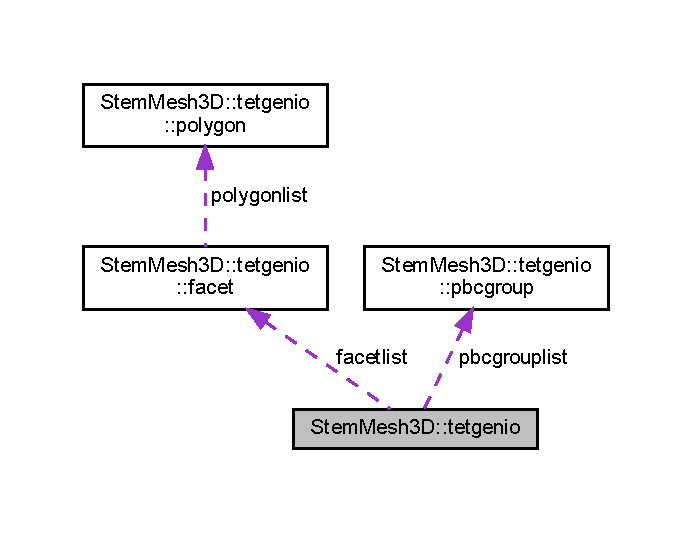
\includegraphics[width=332pt]{classStemMesh3D_1_1tetgenio__coll__graph}
\end{center}
\end{figure}
\doxysubsection*{Classes}
\begin{DoxyCompactItemize}
\item 
struct \mbox{\hyperlink{structStemMesh3D_1_1tetgenio_1_1facet}{facet}}
\item 
struct \mbox{\hyperlink{structStemMesh3D_1_1tetgenio_1_1pbcgroup}{pbcgroup}}
\item 
struct \mbox{\hyperlink{structStemMesh3D_1_1tetgenio_1_1polygon}{polygon}}
\end{DoxyCompactItemize}
\doxysubsection*{Public Types}
\begin{DoxyCompactItemize}
\item 
\mbox{\Hypertarget{classStemMesh3D_1_1tetgenio_aeb3b8945a91f73d771453de7760d523a}\label{classStemMesh3D_1_1tetgenio_aeb3b8945a91f73d771453de7760d523a}} 
enum \{ {\bfseries F\+I\+L\+E\+N\+A\+M\+E\+S\+I\+ZE} = 1024
 \}
\item 
\mbox{\Hypertarget{classStemMesh3D_1_1tetgenio_a774bcf24d97d570a2a74d762a789b89e}\label{classStemMesh3D_1_1tetgenio_a774bcf24d97d570a2a74d762a789b89e}} 
enum \{ {\bfseries I\+N\+P\+U\+T\+L\+I\+N\+E\+S\+I\+ZE} = 1024
 \}
\end{DoxyCompactItemize}
\doxysubsection*{Public Member Functions}
\begin{DoxyCompactItemize}
\item 
\mbox{\Hypertarget{classStemMesh3D_1_1tetgenio_ac16e6ad18ce273e5641e77e43133ab34}\label{classStemMesh3D_1_1tetgenio_ac16e6ad18ce273e5641e77e43133ab34}} 
void {\bfseries initialize} ()
\item 
\mbox{\Hypertarget{classStemMesh3D_1_1tetgenio_a50791238a7e9e271328b5c80cb48cced}\label{classStemMesh3D_1_1tetgenio_a50791238a7e9e271328b5c80cb48cced}} 
void {\bfseries deinitialize} ()
\item 
\mbox{\Hypertarget{classStemMesh3D_1_1tetgenio_a1d2641699dddb6a716635f43de307586}\label{classStemMesh3D_1_1tetgenio_a1d2641699dddb6a716635f43de307586}} 
bool {\bfseries load\+\_\+node\+\_\+call} (F\+I\+LE $\ast$infile, int markers, char $\ast$nodefilename)
\item 
\mbox{\Hypertarget{classStemMesh3D_1_1tetgenio_a329156308b8f67251fc4490dc8e6d983}\label{classStemMesh3D_1_1tetgenio_a329156308b8f67251fc4490dc8e6d983}} 
bool {\bfseries load\+\_\+node} (char $\ast$filename)
\item 
\mbox{\Hypertarget{classStemMesh3D_1_1tetgenio_a1d6cd4aacd1fafe1f9522be663e503c4}\label{classStemMesh3D_1_1tetgenio_a1d6cd4aacd1fafe1f9522be663e503c4}} 
bool {\bfseries load\+\_\+addnodes} (char $\ast$filename)
\item 
\mbox{\Hypertarget{classStemMesh3D_1_1tetgenio_a83442e24a49527ea42e7af8d1d800b33}\label{classStemMesh3D_1_1tetgenio_a83442e24a49527ea42e7af8d1d800b33}} 
bool {\bfseries load\+\_\+pbc} (char $\ast$filename)
\item 
\mbox{\Hypertarget{classStemMesh3D_1_1tetgenio_aa75ecd50869344069c8aab5bdd3b0e35}\label{classStemMesh3D_1_1tetgenio_aa75ecd50869344069c8aab5bdd3b0e35}} 
bool {\bfseries load\+\_\+var} (char $\ast$filename)
\item 
\mbox{\Hypertarget{classStemMesh3D_1_1tetgenio_a6eb2fe04559b4a56c574cd39c8e34439}\label{classStemMesh3D_1_1tetgenio_a6eb2fe04559b4a56c574cd39c8e34439}} 
bool {\bfseries load\+\_\+poly} (char $\ast$filename)
\item 
\mbox{\Hypertarget{classStemMesh3D_1_1tetgenio_aeaf98f93edbd2a9faa0d53ff4bc4e91b}\label{classStemMesh3D_1_1tetgenio_aeaf98f93edbd2a9faa0d53ff4bc4e91b}} 
bool {\bfseries load\+\_\+off} (char $\ast$filename)
\item 
\mbox{\Hypertarget{classStemMesh3D_1_1tetgenio_ad22ac047eb377f5ab2fd84c0bee395cd}\label{classStemMesh3D_1_1tetgenio_ad22ac047eb377f5ab2fd84c0bee395cd}} 
bool {\bfseries load\+\_\+ply} (char $\ast$filename)
\item 
\mbox{\Hypertarget{classStemMesh3D_1_1tetgenio_a1f26b5156c03a480c264bdec1c1b2bfa}\label{classStemMesh3D_1_1tetgenio_a1f26b5156c03a480c264bdec1c1b2bfa}} 
bool {\bfseries load\+\_\+stl} (char $\ast$filename)
\item 
\mbox{\Hypertarget{classStemMesh3D_1_1tetgenio_aa4bdbd3ea2da2914e24c67be7e6d1d0a}\label{classStemMesh3D_1_1tetgenio_aa4bdbd3ea2da2914e24c67be7e6d1d0a}} 
bool {\bfseries load\+\_\+medit} (char $\ast$filename)
\item 
\mbox{\Hypertarget{classStemMesh3D_1_1tetgenio_ad327410b2ab83ec06860a141a4e87a7f}\label{classStemMesh3D_1_1tetgenio_ad327410b2ab83ec06860a141a4e87a7f}} 
bool {\bfseries load\+\_\+plc} (char $\ast$filename, int object)
\item 
\mbox{\Hypertarget{classStemMesh3D_1_1tetgenio_a198f47cd3bd717057bc0f22d5dcf4b5b}\label{classStemMesh3D_1_1tetgenio_a198f47cd3bd717057bc0f22d5dcf4b5b}} 
bool {\bfseries load\+\_\+tetmesh} (char $\ast$filename)
\item 
\mbox{\Hypertarget{classStemMesh3D_1_1tetgenio_ae2947260644bf6185ca299b31bf90fbf}\label{classStemMesh3D_1_1tetgenio_ae2947260644bf6185ca299b31bf90fbf}} 
void {\bfseries save\+\_\+nodes} (char $\ast$filename)
\item 
\mbox{\Hypertarget{classStemMesh3D_1_1tetgenio_acf84c62877b2201366f0d657b657d358}\label{classStemMesh3D_1_1tetgenio_acf84c62877b2201366f0d657b657d358}} 
void {\bfseries save\+\_\+elements} (char $\ast$filename)
\item 
\mbox{\Hypertarget{classStemMesh3D_1_1tetgenio_a5fee06b57903ebde470e79317b45c65b}\label{classStemMesh3D_1_1tetgenio_a5fee06b57903ebde470e79317b45c65b}} 
void {\bfseries save\+\_\+faces} (char $\ast$filename)
\item 
\mbox{\Hypertarget{classStemMesh3D_1_1tetgenio_aa90ff0a1c24587809f9c0b537aa66db7}\label{classStemMesh3D_1_1tetgenio_aa90ff0a1c24587809f9c0b537aa66db7}} 
void {\bfseries save\+\_\+edges} (char $\ast$filename)
\item 
\mbox{\Hypertarget{classStemMesh3D_1_1tetgenio_a57cf97fce145ff0a66725ea93c556e5c}\label{classStemMesh3D_1_1tetgenio_a57cf97fce145ff0a66725ea93c556e5c}} 
void {\bfseries save\+\_\+neighbors} (char $\ast$filename)
\item 
\mbox{\Hypertarget{classStemMesh3D_1_1tetgenio_a88932d9ac915a7d594022da818fca634}\label{classStemMesh3D_1_1tetgenio_a88932d9ac915a7d594022da818fca634}} 
void {\bfseries save\+\_\+poly} (char $\ast$filename)
\item 
\mbox{\Hypertarget{classStemMesh3D_1_1tetgenio_a03cd753e6b48b419d538bfb48b87469c}\label{classStemMesh3D_1_1tetgenio_a03cd753e6b48b419d538bfb48b87469c}} 
char $\ast$ {\bfseries readline} (char $\ast$string, F\+I\+LE $\ast$infile, int $\ast$linenumber)
\item 
\mbox{\Hypertarget{classStemMesh3D_1_1tetgenio_a63cd8cf14961e8cafa5a543c7bf651b4}\label{classStemMesh3D_1_1tetgenio_a63cd8cf14961e8cafa5a543c7bf651b4}} 
char $\ast$ {\bfseries findnextfield} (char $\ast$string)
\item 
\mbox{\Hypertarget{classStemMesh3D_1_1tetgenio_a12755b132e01188103f40384f7cc5a9d}\label{classStemMesh3D_1_1tetgenio_a12755b132e01188103f40384f7cc5a9d}} 
char $\ast$ {\bfseries readnumberline} (char $\ast$string, F\+I\+LE $\ast$infile, char $\ast$infilename)
\item 
\mbox{\Hypertarget{classStemMesh3D_1_1tetgenio_a35197f177bf5ffd75c181c245d2c4b36}\label{classStemMesh3D_1_1tetgenio_a35197f177bf5ffd75c181c245d2c4b36}} 
char $\ast$ {\bfseries findnextnumber} (char $\ast$string)
\end{DoxyCompactItemize}
\doxysubsection*{Static Public Member Functions}
\begin{DoxyCompactItemize}
\item 
\mbox{\Hypertarget{classStemMesh3D_1_1tetgenio_aad465116bd4a3b81668f09ca639545d8}\label{classStemMesh3D_1_1tetgenio_aad465116bd4a3b81668f09ca639545d8}} 
static void {\bfseries init} (\mbox{\hyperlink{structStemMesh3D_1_1tetgenio_1_1polygon}{polygon}} $\ast$p)
\item 
\mbox{\Hypertarget{classStemMesh3D_1_1tetgenio_a82b49bf2fe508832efb12cf290b74d17}\label{classStemMesh3D_1_1tetgenio_a82b49bf2fe508832efb12cf290b74d17}} 
static void {\bfseries init} (\mbox{\hyperlink{structStemMesh3D_1_1tetgenio_1_1facet}{facet}} $\ast$f)
\end{DoxyCompactItemize}
\doxysubsection*{Public Attributes}
\begin{DoxyCompactItemize}
\item 
\mbox{\Hypertarget{classStemMesh3D_1_1tetgenio_a09e3de45049962cc14a8383f823a08f7}\label{classStemMesh3D_1_1tetgenio_a09e3de45049962cc14a8383f823a08f7}} 
int {\bfseries firstnumber}
\item 
\mbox{\Hypertarget{classStemMesh3D_1_1tetgenio_aa3de1ebb0258d2e2af7e2441c7d0fffa}\label{classStemMesh3D_1_1tetgenio_aa3de1ebb0258d2e2af7e2441c7d0fffa}} 
int {\bfseries mesh\+\_\+dim}
\item 
\mbox{\Hypertarget{classStemMesh3D_1_1tetgenio_a6ff6107d87bb86a2035154cc6085ce43}\label{classStemMesh3D_1_1tetgenio_a6ff6107d87bb86a2035154cc6085ce43}} 
R\+E\+AL $\ast$ {\bfseries pointlist}
\item 
\mbox{\Hypertarget{classStemMesh3D_1_1tetgenio_ab24affc4b9d372ba0ba192af5f4bbcf3}\label{classStemMesh3D_1_1tetgenio_ab24affc4b9d372ba0ba192af5f4bbcf3}} 
R\+E\+AL $\ast$ {\bfseries pointattributelist}
\item 
\mbox{\Hypertarget{classStemMesh3D_1_1tetgenio_a914e829ba35daebbc51a35f430db92e3}\label{classStemMesh3D_1_1tetgenio_a914e829ba35daebbc51a35f430db92e3}} 
R\+E\+AL $\ast$ {\bfseries addpointlist}
\item 
\mbox{\Hypertarget{classStemMesh3D_1_1tetgenio_ad13c2e982e8a7a5b679327d79f4139a4}\label{classStemMesh3D_1_1tetgenio_ad13c2e982e8a7a5b679327d79f4139a4}} 
int $\ast$ {\bfseries pointmarkerlist}
\item 
\mbox{\Hypertarget{classStemMesh3D_1_1tetgenio_aeb14ac64946c796c4fd1c12c178a1908}\label{classStemMesh3D_1_1tetgenio_aeb14ac64946c796c4fd1c12c178a1908}} 
int {\bfseries numberofpoints}
\item 
\mbox{\Hypertarget{classStemMesh3D_1_1tetgenio_a6db73e75cd77d1e4f3d18ca96b873b17}\label{classStemMesh3D_1_1tetgenio_a6db73e75cd77d1e4f3d18ca96b873b17}} 
int {\bfseries numberofpointattributes}
\item 
\mbox{\Hypertarget{classStemMesh3D_1_1tetgenio_ac16549f431847564e2c1340fae5eb5fe}\label{classStemMesh3D_1_1tetgenio_ac16549f431847564e2c1340fae5eb5fe}} 
int {\bfseries numberofaddpoints}
\item 
\mbox{\Hypertarget{classStemMesh3D_1_1tetgenio_a02976bf5fc92eb8f11c7b0dcaef25c7a}\label{classStemMesh3D_1_1tetgenio_a02976bf5fc92eb8f11c7b0dcaef25c7a}} 
int $\ast$ {\bfseries tetrahedronlist}
\item 
\mbox{\Hypertarget{classStemMesh3D_1_1tetgenio_adfacf997837300183a9e066a25df94a4}\label{classStemMesh3D_1_1tetgenio_adfacf997837300183a9e066a25df94a4}} 
R\+E\+AL $\ast$ {\bfseries tetrahedronattributelist}
\item 
\mbox{\Hypertarget{classStemMesh3D_1_1tetgenio_acb22b561061050986f40838c45686ef3}\label{classStemMesh3D_1_1tetgenio_acb22b561061050986f40838c45686ef3}} 
R\+E\+AL $\ast$ {\bfseries tetrahedronvolumelist}
\item 
\mbox{\Hypertarget{classStemMesh3D_1_1tetgenio_aef899cc17366c00494c2b9fbb2c10f63}\label{classStemMesh3D_1_1tetgenio_aef899cc17366c00494c2b9fbb2c10f63}} 
int $\ast$ {\bfseries neighborlist}
\item 
\mbox{\Hypertarget{classStemMesh3D_1_1tetgenio_a23dbe000145eff15daf4e30967dbc509}\label{classStemMesh3D_1_1tetgenio_a23dbe000145eff15daf4e30967dbc509}} 
int {\bfseries numberoftetrahedra}
\item 
\mbox{\Hypertarget{classStemMesh3D_1_1tetgenio_a8f66b00bf6545aacdbfb761128983bd9}\label{classStemMesh3D_1_1tetgenio_a8f66b00bf6545aacdbfb761128983bd9}} 
int {\bfseries numberofcorners}
\item 
\mbox{\Hypertarget{classStemMesh3D_1_1tetgenio_ab740c7ceee2ffdc278914bdeb0f20bb0}\label{classStemMesh3D_1_1tetgenio_ab740c7ceee2ffdc278914bdeb0f20bb0}} 
int {\bfseries numberoftetrahedronattributes}
\item 
\mbox{\Hypertarget{classStemMesh3D_1_1tetgenio_afeae0cef633dea221713fee929b28599}\label{classStemMesh3D_1_1tetgenio_afeae0cef633dea221713fee929b28599}} 
\mbox{\hyperlink{structStemMesh3D_1_1tetgenio_1_1facet}{facet}} $\ast$ {\bfseries facetlist}
\item 
\mbox{\Hypertarget{classStemMesh3D_1_1tetgenio_a1c8e862919b79e311087732efe534cd3}\label{classStemMesh3D_1_1tetgenio_a1c8e862919b79e311087732efe534cd3}} 
int $\ast$ {\bfseries facetmarkerlist}
\item 
\mbox{\Hypertarget{classStemMesh3D_1_1tetgenio_af445f0d9f30d5bc74fa175c6d14cb2ee}\label{classStemMesh3D_1_1tetgenio_af445f0d9f30d5bc74fa175c6d14cb2ee}} 
int {\bfseries numberoffacets}
\item 
\mbox{\Hypertarget{classStemMesh3D_1_1tetgenio_a8b86ed43b82ae7bd4e4c749bff9d57ae}\label{classStemMesh3D_1_1tetgenio_a8b86ed43b82ae7bd4e4c749bff9d57ae}} 
R\+E\+AL $\ast$ {\bfseries holelist}
\item 
\mbox{\Hypertarget{classStemMesh3D_1_1tetgenio_a095291ec7bc07a1c9da094be8b8fe5e5}\label{classStemMesh3D_1_1tetgenio_a095291ec7bc07a1c9da094be8b8fe5e5}} 
int {\bfseries numberofholes}
\item 
\mbox{\Hypertarget{classStemMesh3D_1_1tetgenio_a5914729a9415f08207f5b43dfb4d154d}\label{classStemMesh3D_1_1tetgenio_a5914729a9415f08207f5b43dfb4d154d}} 
R\+E\+AL $\ast$ {\bfseries regionlist}
\item 
\mbox{\Hypertarget{classStemMesh3D_1_1tetgenio_a3ef1ef2de691c018f2c89d3eef859379}\label{classStemMesh3D_1_1tetgenio_a3ef1ef2de691c018f2c89d3eef859379}} 
int {\bfseries numberofregions}
\item 
\mbox{\Hypertarget{classStemMesh3D_1_1tetgenio_a53e2f2cfcf8fd462c6bd9ee606d10d66}\label{classStemMesh3D_1_1tetgenio_a53e2f2cfcf8fd462c6bd9ee606d10d66}} 
R\+E\+AL $\ast$ {\bfseries facetconstraintlist}
\item 
\mbox{\Hypertarget{classStemMesh3D_1_1tetgenio_a8868e0398d33c68a859c93fdd16c89ed}\label{classStemMesh3D_1_1tetgenio_a8868e0398d33c68a859c93fdd16c89ed}} 
int {\bfseries numberoffacetconstraints}
\item 
\mbox{\Hypertarget{classStemMesh3D_1_1tetgenio_a197a69132226c424c1dded9bf3ca9023}\label{classStemMesh3D_1_1tetgenio_a197a69132226c424c1dded9bf3ca9023}} 
R\+E\+AL $\ast$ {\bfseries segmentconstraintlist}
\item 
\mbox{\Hypertarget{classStemMesh3D_1_1tetgenio_aef0f2b92e42626444cefe887888007d5}\label{classStemMesh3D_1_1tetgenio_aef0f2b92e42626444cefe887888007d5}} 
int {\bfseries numberofsegmentconstraints}
\item 
\mbox{\Hypertarget{classStemMesh3D_1_1tetgenio_a760b23d98f9f067a54f0b2101ef36b4d}\label{classStemMesh3D_1_1tetgenio_a760b23d98f9f067a54f0b2101ef36b4d}} 
R\+E\+AL $\ast$ {\bfseries nodeconstraintlist}
\item 
\mbox{\Hypertarget{classStemMesh3D_1_1tetgenio_a09616a7d15879c9e6068b6381eea8f0b}\label{classStemMesh3D_1_1tetgenio_a09616a7d15879c9e6068b6381eea8f0b}} 
int {\bfseries numberofnodeconstraints}
\item 
\mbox{\Hypertarget{classStemMesh3D_1_1tetgenio_a7cb0773b4e9be518644b4dc29b213b16}\label{classStemMesh3D_1_1tetgenio_a7cb0773b4e9be518644b4dc29b213b16}} 
\mbox{\hyperlink{structStemMesh3D_1_1tetgenio_1_1pbcgroup}{pbcgroup}} $\ast$ {\bfseries pbcgrouplist}
\item 
\mbox{\Hypertarget{classStemMesh3D_1_1tetgenio_a0cea787d5f18130cecbb14cd485a31a9}\label{classStemMesh3D_1_1tetgenio_a0cea787d5f18130cecbb14cd485a31a9}} 
int {\bfseries numberofpbcgroups}
\item 
\mbox{\Hypertarget{classStemMesh3D_1_1tetgenio_a845cc1a4a1e3b95c0fe1cf37c7c1de1a}\label{classStemMesh3D_1_1tetgenio_a845cc1a4a1e3b95c0fe1cf37c7c1de1a}} 
int $\ast$ {\bfseries trifacelist}
\item 
\mbox{\Hypertarget{classStemMesh3D_1_1tetgenio_a5e7a5d11d168251f7d5ba8794f13fe42}\label{classStemMesh3D_1_1tetgenio_a5e7a5d11d168251f7d5ba8794f13fe42}} 
int $\ast$ {\bfseries trifacemarkerlist}
\item 
\mbox{\Hypertarget{classStemMesh3D_1_1tetgenio_a5555ba8f8337eb339d0fe2d7decd3475}\label{classStemMesh3D_1_1tetgenio_a5555ba8f8337eb339d0fe2d7decd3475}} 
int {\bfseries numberoftrifaces}
\item 
\mbox{\Hypertarget{classStemMesh3D_1_1tetgenio_af075e154234bb4975355f6a6ade72b0a}\label{classStemMesh3D_1_1tetgenio_af075e154234bb4975355f6a6ade72b0a}} 
int $\ast$ {\bfseries edgelist}
\item 
\mbox{\Hypertarget{classStemMesh3D_1_1tetgenio_accedc23de3f2aa2a567a9ee7560819d5}\label{classStemMesh3D_1_1tetgenio_accedc23de3f2aa2a567a9ee7560819d5}} 
int $\ast$ {\bfseries edgemarkerlist}
\item 
\mbox{\Hypertarget{classStemMesh3D_1_1tetgenio_a12a7d8064cd6a20c386d69d65ba37ffd}\label{classStemMesh3D_1_1tetgenio_a12a7d8064cd6a20c386d69d65ba37ffd}} 
int {\bfseries numberofedges}
\end{DoxyCompactItemize}


The documentation for this class was generated from the following file\+:\begin{DoxyCompactItemize}
\item 
src/\+Mesh/\+Stem\+Mesh/tetgen.\+h\end{DoxyCompactItemize}

\hypertarget{classStemMesh3D_1_1tetgenmesh}{}\section{Stem\+Mesh3D\+:\+:tetgenmesh Class Reference}
\label{classStemMesh3D_1_1tetgenmesh}\index{Stem\+Mesh3\+D\+::tetgenmesh@{Stem\+Mesh3\+D\+::tetgenmesh}}


Collaboration diagram for Stem\+Mesh3D\+:\+:tetgenmesh\+:\nopagebreak
\begin{figure}[H]
\begin{center}
\leavevmode
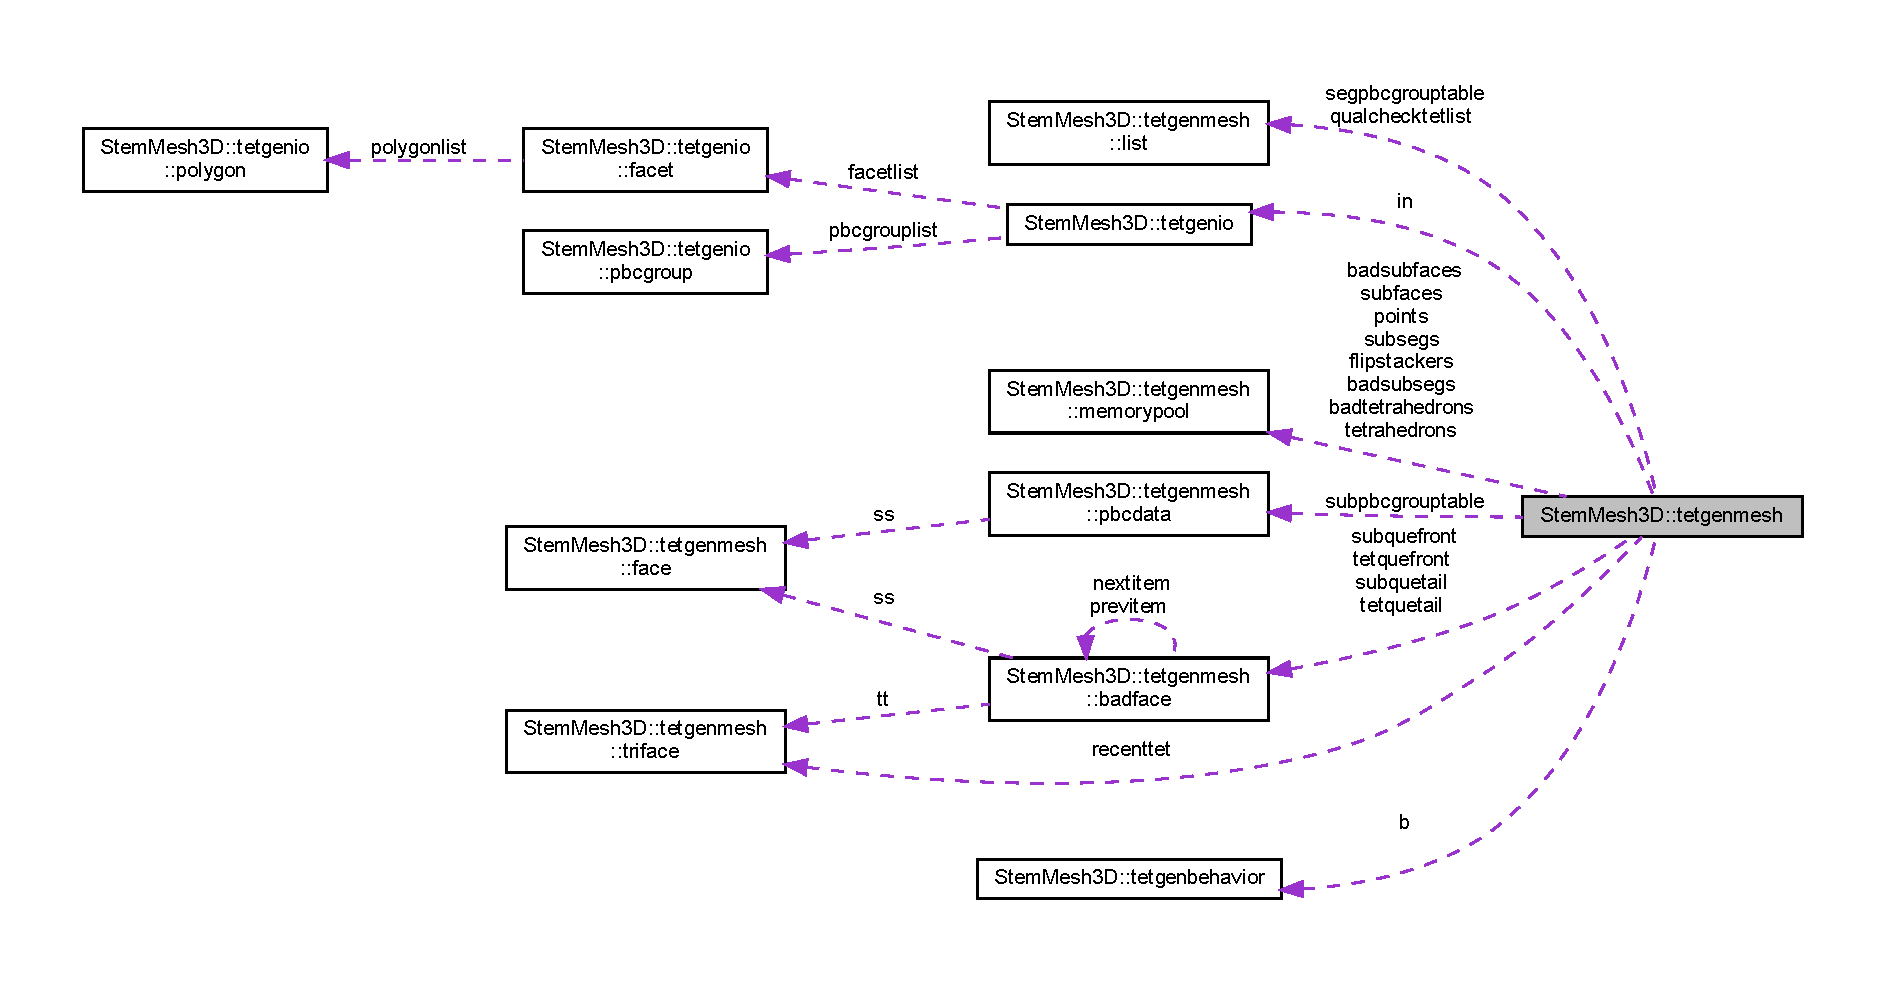
\includegraphics[width=350pt]{classStemMesh3D_1_1tetgenmesh__coll__graph}
\end{center}
\end{figure}
\subsection*{Classes}
\begin{DoxyCompactItemize}
\item 
struct \hyperlink{structStemMesh3D_1_1tetgenmesh_1_1badface}{badface}
\item 
class \hyperlink{classStemMesh3D_1_1tetgenmesh_1_1face}{face}
\item 
class \hyperlink{classStemMesh3D_1_1tetgenmesh_1_1link}{link}
\item 
class \hyperlink{classStemMesh3D_1_1tetgenmesh_1_1list}{list}
\item 
class \hyperlink{classStemMesh3D_1_1tetgenmesh_1_1memorypool}{memorypool}
\item 
struct \hyperlink{structStemMesh3D_1_1tetgenmesh_1_1pbcdata}{pbcdata}
\item 
class \hyperlink{classStemMesh3D_1_1tetgenmesh_1_1queue}{queue}
\item 
class \hyperlink{classStemMesh3D_1_1tetgenmesh_1_1triface}{triface}
\end{DoxyCompactItemize}
\subsection*{Public Types}
\begin{DoxyCompactItemize}
\item 
\mbox{\Hypertarget{classStemMesh3D_1_1tetgenmesh_a47b2d5b741c5d1f3aea8b765aced9d3b}\label{classStemMesh3D_1_1tetgenmesh_a47b2d5b741c5d1f3aea8b765aced9d3b}} 
enum \{ {\bfseries F\+I\+L\+E\+N\+A\+M\+E\+S\+I\+ZE} = 1024
 \}
\item 
\mbox{\Hypertarget{classStemMesh3D_1_1tetgenmesh_a9dcc9d790f721d7a0f4f09a84e9441fb}\label{classStemMesh3D_1_1tetgenmesh_a9dcc9d790f721d7a0f4f09a84e9441fb}} 
enum \{ {\bfseries V\+E\+R\+P\+E\+R\+B\+L\+O\+CK} = 4092, 
{\bfseries S\+U\+B\+P\+E\+R\+B\+L\+O\+CK} = 4092, 
{\bfseries E\+L\+E\+P\+E\+R\+B\+L\+O\+CK} = 8188
 \}
\item 
\mbox{\Hypertarget{classStemMesh3D_1_1tetgenmesh_a5d911914e7f049039ad318a4fc5c5e2b}\label{classStemMesh3D_1_1tetgenmesh_a5d911914e7f049039ad318a4fc5c5e2b}} 
enum \{ {\bfseries S\+A\+M\+P\+L\+E\+F\+A\+C\+T\+OR} = 11
 \}
\item 
\mbox{\Hypertarget{classStemMesh3D_1_1tetgenmesh_a5af38261548ab74f0e5f4b8e070972cc}\label{classStemMesh3D_1_1tetgenmesh_a5af38261548ab74f0e5f4b8e070972cc}} 
enum \{ {\bfseries C\+CW} = 0, 
{\bfseries CW} = 1
 \}
\item 
\mbox{\Hypertarget{classStemMesh3D_1_1tetgenmesh_a1abc5c68feadf753aa1d4c0a50c987a5}\label{classStemMesh3D_1_1tetgenmesh_a1abc5c68feadf753aa1d4c0a50c987a5}} 
enum {\bfseries wordtype} \{ {\bfseries P\+O\+I\+N\+T\+ER}, 
{\bfseries F\+L\+O\+A\+T\+I\+N\+G\+P\+O\+I\+NT}
 \}
\item 
\mbox{\Hypertarget{classStemMesh3D_1_1tetgenmesh_a009cb173727c930b7e64c0fa3959bcf4}\label{classStemMesh3D_1_1tetgenmesh_a009cb173727c930b7e64c0fa3959bcf4}} 
enum {\bfseries verttype} \{ \newline
{\bfseries U\+N\+U\+S\+E\+D\+V\+E\+R\+T\+EX}, 
{\bfseries D\+U\+P\+L\+I\+C\+A\+T\+E\+D\+V\+E\+R\+T\+EX}, 
{\bfseries N\+A\+C\+U\+T\+E\+V\+E\+R\+T\+EX}, 
{\bfseries A\+C\+U\+T\+E\+V\+E\+R\+T\+EX}, 
\newline
{\bfseries F\+R\+E\+E\+S\+E\+G\+V\+E\+R\+T\+EX}, 
{\bfseries F\+A\+C\+E\+T\+V\+E\+R\+T\+EX}, 
{\bfseries F\+R\+E\+E\+S\+U\+B\+V\+E\+R\+T\+EX}, 
{\bfseries F\+R\+E\+E\+V\+O\+L\+V\+E\+R\+T\+EX}, 
\newline
{\bfseries D\+E\+A\+D\+V\+E\+R\+T\+EX} = -\/32768
 \}
\item 
\mbox{\Hypertarget{classStemMesh3D_1_1tetgenmesh_aafead8788dd843fd3fde0bb5af3e19c5}\label{classStemMesh3D_1_1tetgenmesh_aafead8788dd843fd3fde0bb5af3e19c5}} 
enum {\bfseries shestype} \{ {\bfseries N\+S\+H\+A\+R\+P\+N\+S\+K\+I\+N\+NY}, 
{\bfseries S\+H\+A\+R\+P\+S\+UB}, 
{\bfseries S\+K\+I\+N\+N\+Y\+S\+UB}, 
{\bfseries S\+H\+A\+R\+P\+S\+K\+I\+N\+N\+Y\+S\+UB}
 \}
\item 
\mbox{\Hypertarget{classStemMesh3D_1_1tetgenmesh_a145df1bb5469ef9750bbd4ffc4baf65b}\label{classStemMesh3D_1_1tetgenmesh_a145df1bb5469ef9750bbd4ffc4baf65b}} 
enum {\bfseries fliptype} \{ \newline
{\bfseries T23}, 
{\bfseries T32}, 
{\bfseries T22}, 
{\bfseries T44}, 
\newline
{\bfseries U\+N\+F\+L\+I\+P\+A\+B\+LE}, 
{\bfseries F\+O\+R\+B\+I\+D\+D\+E\+N\+F\+A\+CE}, 
{\bfseries F\+O\+R\+B\+I\+D\+D\+E\+N\+E\+D\+GE}, 
{\bfseries N\+O\+N\+C\+O\+N\+V\+EX}
 \}
\item 
\mbox{\Hypertarget{classStemMesh3D_1_1tetgenmesh_a932fad29c9c281acfcd84f5e9b985408}\label{classStemMesh3D_1_1tetgenmesh_a932fad29c9c281acfcd84f5e9b985408}} 
enum {\bfseries interresult} \{ \newline
{\bfseries D\+I\+S\+J\+O\+I\+NT}, 
{\bfseries S\+H\+A\+R\+E\+V\+E\+R\+T\+EX}, 
{\bfseries S\+H\+A\+R\+E\+E\+D\+GE}, 
{\bfseries S\+H\+A\+R\+E\+F\+A\+CE}, 
\newline
{\bfseries I\+N\+T\+E\+R\+S\+E\+CT}
 \}
\item 
\mbox{\Hypertarget{classStemMesh3D_1_1tetgenmesh_a20ef79c6bd4980b3c1771dfc2c86899a}\label{classStemMesh3D_1_1tetgenmesh_a20ef79c6bd4980b3c1771dfc2c86899a}} 
enum {\bfseries locateresult} \{ \newline
{\bfseries I\+N\+T\+E\+T\+R\+A\+H\+E\+D\+R\+ON}, 
{\bfseries O\+N\+F\+A\+CE}, 
{\bfseries O\+N\+E\+D\+GE}, 
{\bfseries O\+N\+V\+E\+R\+T\+EX}, 
\newline
{\bfseries O\+U\+T\+S\+I\+DE}
 \}
\item 
\mbox{\Hypertarget{classStemMesh3D_1_1tetgenmesh_a573b108b3b86818997fda0af829d1471}\label{classStemMesh3D_1_1tetgenmesh_a573b108b3b86818997fda0af829d1471}} 
enum {\bfseries insertsiteresult} \{ \newline
{\bfseries S\+U\+C\+C\+E\+S\+S\+I\+N\+T\+ET}, 
{\bfseries S\+U\+C\+C\+E\+S\+S\+O\+N\+F\+A\+CE}, 
{\bfseries S\+U\+C\+C\+E\+S\+S\+O\+N\+E\+D\+GE}, 
{\bfseries D\+U\+P\+L\+I\+C\+A\+T\+E\+P\+O\+I\+NT}, 
\newline
{\bfseries O\+U\+T\+S\+I\+D\+E\+P\+O\+I\+NT}
 \}
\item 
\mbox{\Hypertarget{classStemMesh3D_1_1tetgenmesh_a569afa21157dde381da3156e4f9ba377}\label{classStemMesh3D_1_1tetgenmesh_a569afa21157dde381da3156e4f9ba377}} 
enum {\bfseries finddirectionresult} \{ \newline
{\bfseries A\+C\+R\+O\+S\+S\+E\+D\+GE}, 
{\bfseries A\+C\+R\+O\+S\+S\+F\+A\+CE}, 
{\bfseries L\+E\+F\+T\+C\+O\+L\+L\+I\+N\+E\+AR}, 
{\bfseries R\+I\+G\+H\+T\+C\+O\+L\+L\+I\+N\+E\+AR}, 
\newline
{\bfseries T\+O\+P\+C\+O\+L\+L\+I\+N\+E\+AR}, 
{\bfseries B\+E\+L\+O\+W\+H\+U\+LL}
 \}
\item 
\mbox{\Hypertarget{classStemMesh3D_1_1tetgenmesh_a0b0a0adbcf9f3ce0befe5bfbc491ed07}\label{classStemMesh3D_1_1tetgenmesh_a0b0a0adbcf9f3ce0befe5bfbc491ed07}} 
typedef R\+E\+AL $\ast$$\ast$ {\bfseries tetrahedron}
\item 
\mbox{\Hypertarget{classStemMesh3D_1_1tetgenmesh_ae33cf3d2d3f1041b81317cf64abc5d7e}\label{classStemMesh3D_1_1tetgenmesh_ae33cf3d2d3f1041b81317cf64abc5d7e}} 
typedef R\+E\+AL $\ast$$\ast$ {\bfseries shellface}
\item 
\mbox{\Hypertarget{classStemMesh3D_1_1tetgenmesh_a331d48b97ab35ae6e088fd9fe9c9355b}\label{classStemMesh3D_1_1tetgenmesh_a331d48b97ab35ae6e088fd9fe9c9355b}} 
typedef R\+E\+AL $\ast$ {\bfseries point}
\item 
\mbox{\Hypertarget{classStemMesh3D_1_1tetgenmesh_a5899e49ef7c1e04977cae322b3cc6a9b}\label{classStemMesh3D_1_1tetgenmesh_a5899e49ef7c1e04977cae322b3cc6a9b}} 
typedef int($\ast$ {\bfseries compfunc}) (const void $\ast$, const void $\ast$)
\end{DoxyCompactItemize}
\subsection*{Public Member Functions}
\begin{DoxyCompactItemize}
\item 
\mbox{\Hypertarget{classStemMesh3D_1_1tetgenmesh_a46943a0bbb60e6b4a18dff9af049fcdd}\label{classStemMesh3D_1_1tetgenmesh_a46943a0bbb60e6b4a18dff9af049fcdd}} 
void {\bfseries decode} (tetrahedron ptr, \hyperlink{classStemMesh3D_1_1tetgenmesh_1_1triface}{triface} \&t)
\item 
\mbox{\Hypertarget{classStemMesh3D_1_1tetgenmesh_a589d865738934055945b56ca89722997}\label{classStemMesh3D_1_1tetgenmesh_a589d865738934055945b56ca89722997}} 
tetrahedron {\bfseries encode} (\hyperlink{classStemMesh3D_1_1tetgenmesh_1_1triface}{triface} \&t)
\item 
\mbox{\Hypertarget{classStemMesh3D_1_1tetgenmesh_a2684fea0615042e698f9737b41eafa51}\label{classStemMesh3D_1_1tetgenmesh_a2684fea0615042e698f9737b41eafa51}} 
void {\bfseries sym} (\hyperlink{classStemMesh3D_1_1tetgenmesh_1_1triface}{triface} \&t1, \hyperlink{classStemMesh3D_1_1tetgenmesh_1_1triface}{triface} \&t2)
\item 
\mbox{\Hypertarget{classStemMesh3D_1_1tetgenmesh_aa531a3d129e6a9ab1cf8b1722a436e00}\label{classStemMesh3D_1_1tetgenmesh_aa531a3d129e6a9ab1cf8b1722a436e00}} 
void {\bfseries symself} (\hyperlink{classStemMesh3D_1_1tetgenmesh_1_1triface}{triface} \&t)
\item 
\mbox{\Hypertarget{classStemMesh3D_1_1tetgenmesh_a03df2d5f488abcf48f15989bc2789d07}\label{classStemMesh3D_1_1tetgenmesh_a03df2d5f488abcf48f15989bc2789d07}} 
void {\bfseries bond} (\hyperlink{classStemMesh3D_1_1tetgenmesh_1_1triface}{triface} \&t1, \hyperlink{classStemMesh3D_1_1tetgenmesh_1_1triface}{triface} \&t2)
\item 
\mbox{\Hypertarget{classStemMesh3D_1_1tetgenmesh_ab1c47c5bc730b51ba2640b6c3eff5371}\label{classStemMesh3D_1_1tetgenmesh_ab1c47c5bc730b51ba2640b6c3eff5371}} 
void {\bfseries dissolve} (\hyperlink{classStemMesh3D_1_1tetgenmesh_1_1triface}{triface} \&t)
\item 
\mbox{\Hypertarget{classStemMesh3D_1_1tetgenmesh_ac4c574d634e75a37dfbca1d6bf16434c}\label{classStemMesh3D_1_1tetgenmesh_ac4c574d634e75a37dfbca1d6bf16434c}} 
point {\bfseries org} (\hyperlink{classStemMesh3D_1_1tetgenmesh_1_1triface}{triface} \&t)
\item 
\mbox{\Hypertarget{classStemMesh3D_1_1tetgenmesh_a549e4aa7f06866f19303f069a412e6bb}\label{classStemMesh3D_1_1tetgenmesh_a549e4aa7f06866f19303f069a412e6bb}} 
point {\bfseries dest} (\hyperlink{classStemMesh3D_1_1tetgenmesh_1_1triface}{triface} \&t)
\item 
\mbox{\Hypertarget{classStemMesh3D_1_1tetgenmesh_ae40cad42bb9cecfd5e1e9948a08acd6c}\label{classStemMesh3D_1_1tetgenmesh_ae40cad42bb9cecfd5e1e9948a08acd6c}} 
point {\bfseries apex} (\hyperlink{classStemMesh3D_1_1tetgenmesh_1_1triface}{triface} \&t)
\item 
\mbox{\Hypertarget{classStemMesh3D_1_1tetgenmesh_ae4b14b4e0ede00a72e833d017475fc66}\label{classStemMesh3D_1_1tetgenmesh_ae4b14b4e0ede00a72e833d017475fc66}} 
point {\bfseries oppo} (\hyperlink{classStemMesh3D_1_1tetgenmesh_1_1triface}{triface} \&t)
\item 
\mbox{\Hypertarget{classStemMesh3D_1_1tetgenmesh_aff7417f727767a1e335d4bae77234784}\label{classStemMesh3D_1_1tetgenmesh_aff7417f727767a1e335d4bae77234784}} 
void {\bfseries setorg} (\hyperlink{classStemMesh3D_1_1tetgenmesh_1_1triface}{triface} \&t, point pointptr)
\item 
\mbox{\Hypertarget{classStemMesh3D_1_1tetgenmesh_a35f185996bc0a64e00ce05425ed4fb07}\label{classStemMesh3D_1_1tetgenmesh_a35f185996bc0a64e00ce05425ed4fb07}} 
void {\bfseries setdest} (\hyperlink{classStemMesh3D_1_1tetgenmesh_1_1triface}{triface} \&t, point pointptr)
\item 
\mbox{\Hypertarget{classStemMesh3D_1_1tetgenmesh_ad53588986ccb32392fa4c63b29930460}\label{classStemMesh3D_1_1tetgenmesh_ad53588986ccb32392fa4c63b29930460}} 
void {\bfseries setapex} (\hyperlink{classStemMesh3D_1_1tetgenmesh_1_1triface}{triface} \&t, point pointptr)
\item 
\mbox{\Hypertarget{classStemMesh3D_1_1tetgenmesh_a71b84891ff08beb2fbd232cf5eef289c}\label{classStemMesh3D_1_1tetgenmesh_a71b84891ff08beb2fbd232cf5eef289c}} 
void {\bfseries setoppo} (\hyperlink{classStemMesh3D_1_1tetgenmesh_1_1triface}{triface} \&t, point pointptr)
\item 
\mbox{\Hypertarget{classStemMesh3D_1_1tetgenmesh_abb1a8764167d111bb28b2c477253f821}\label{classStemMesh3D_1_1tetgenmesh_abb1a8764167d111bb28b2c477253f821}} 
void {\bfseries esym} (\hyperlink{classStemMesh3D_1_1tetgenmesh_1_1triface}{triface} \&t1, \hyperlink{classStemMesh3D_1_1tetgenmesh_1_1triface}{triface} \&t2)
\item 
\mbox{\Hypertarget{classStemMesh3D_1_1tetgenmesh_a274a1b41f6d795cf64501dbd79c14c76}\label{classStemMesh3D_1_1tetgenmesh_a274a1b41f6d795cf64501dbd79c14c76}} 
void {\bfseries esymself} (\hyperlink{classStemMesh3D_1_1tetgenmesh_1_1triface}{triface} \&t)
\item 
\mbox{\Hypertarget{classStemMesh3D_1_1tetgenmesh_aa7ba526ec257882428d255184bf2acba}\label{classStemMesh3D_1_1tetgenmesh_aa7ba526ec257882428d255184bf2acba}} 
void {\bfseries enext} (\hyperlink{classStemMesh3D_1_1tetgenmesh_1_1triface}{triface} \&t1, \hyperlink{classStemMesh3D_1_1tetgenmesh_1_1triface}{triface} \&t2)
\item 
\mbox{\Hypertarget{classStemMesh3D_1_1tetgenmesh_af68cdb32b3207982b46af556598e7c83}\label{classStemMesh3D_1_1tetgenmesh_af68cdb32b3207982b46af556598e7c83}} 
void {\bfseries enextself} (\hyperlink{classStemMesh3D_1_1tetgenmesh_1_1triface}{triface} \&t)
\item 
\mbox{\Hypertarget{classStemMesh3D_1_1tetgenmesh_adf1997f64633712969fbc59cfb941beb}\label{classStemMesh3D_1_1tetgenmesh_adf1997f64633712969fbc59cfb941beb}} 
void {\bfseries enext2} (\hyperlink{classStemMesh3D_1_1tetgenmesh_1_1triface}{triface} \&t1, \hyperlink{classStemMesh3D_1_1tetgenmesh_1_1triface}{triface} \&t2)
\item 
\mbox{\Hypertarget{classStemMesh3D_1_1tetgenmesh_ab700e2667ed10383ae9b91741d1598ee}\label{classStemMesh3D_1_1tetgenmesh_ab700e2667ed10383ae9b91741d1598ee}} 
void {\bfseries enext2self} (\hyperlink{classStemMesh3D_1_1tetgenmesh_1_1triface}{triface} \&t)
\item 
\mbox{\Hypertarget{classStemMesh3D_1_1tetgenmesh_a053dbc854f45950c4aefbe40a7ced8d8}\label{classStemMesh3D_1_1tetgenmesh_a053dbc854f45950c4aefbe40a7ced8d8}} 
bool {\bfseries fnext} (\hyperlink{classStemMesh3D_1_1tetgenmesh_1_1triface}{triface} \&t1, \hyperlink{classStemMesh3D_1_1tetgenmesh_1_1triface}{triface} \&t2)
\item 
\mbox{\Hypertarget{classStemMesh3D_1_1tetgenmesh_a7f0c17e59000e0381c28b5fb5b8802f3}\label{classStemMesh3D_1_1tetgenmesh_a7f0c17e59000e0381c28b5fb5b8802f3}} 
bool {\bfseries fnextself} (\hyperlink{classStemMesh3D_1_1tetgenmesh_1_1triface}{triface} \&t)
\item 
\mbox{\Hypertarget{classStemMesh3D_1_1tetgenmesh_a6593c944929ab4ff47adaa05884ea7c8}\label{classStemMesh3D_1_1tetgenmesh_a6593c944929ab4ff47adaa05884ea7c8}} 
void {\bfseries enextfnext} (\hyperlink{classStemMesh3D_1_1tetgenmesh_1_1triface}{triface} \&t1, \hyperlink{classStemMesh3D_1_1tetgenmesh_1_1triface}{triface} \&t2)
\item 
\mbox{\Hypertarget{classStemMesh3D_1_1tetgenmesh_a88aff67489fe1e74235e7b5902b32218}\label{classStemMesh3D_1_1tetgenmesh_a88aff67489fe1e74235e7b5902b32218}} 
void {\bfseries enextfnextself} (\hyperlink{classStemMesh3D_1_1tetgenmesh_1_1triface}{triface} \&t)
\item 
\mbox{\Hypertarget{classStemMesh3D_1_1tetgenmesh_ad04ba2e90cfc0064f9415d4b094f8ca4}\label{classStemMesh3D_1_1tetgenmesh_ad04ba2e90cfc0064f9415d4b094f8ca4}} 
void {\bfseries enext2fnext} (\hyperlink{classStemMesh3D_1_1tetgenmesh_1_1triface}{triface} \&t1, \hyperlink{classStemMesh3D_1_1tetgenmesh_1_1triface}{triface} \&t2)
\item 
\mbox{\Hypertarget{classStemMesh3D_1_1tetgenmesh_a34a06e6b0d4a93a1b3f54d75aa8cc033}\label{classStemMesh3D_1_1tetgenmesh_a34a06e6b0d4a93a1b3f54d75aa8cc033}} 
void {\bfseries enext2fnextself} (\hyperlink{classStemMesh3D_1_1tetgenmesh_1_1triface}{triface} \&t)
\item 
\mbox{\Hypertarget{classStemMesh3D_1_1tetgenmesh_aeb796a6233ac4999cac53fc3930fbb31}\label{classStemMesh3D_1_1tetgenmesh_aeb796a6233ac4999cac53fc3930fbb31}} 
void {\bfseries infect} (\hyperlink{classStemMesh3D_1_1tetgenmesh_1_1triface}{triface} \&t)
\item 
\mbox{\Hypertarget{classStemMesh3D_1_1tetgenmesh_aa1795afad705d59babceaf969de46273}\label{classStemMesh3D_1_1tetgenmesh_aa1795afad705d59babceaf969de46273}} 
void {\bfseries uninfect} (\hyperlink{classStemMesh3D_1_1tetgenmesh_1_1triface}{triface} \&t)
\item 
\mbox{\Hypertarget{classStemMesh3D_1_1tetgenmesh_a8898eaf29be7504819db306e70544715}\label{classStemMesh3D_1_1tetgenmesh_a8898eaf29be7504819db306e70544715}} 
bool {\bfseries infected} (\hyperlink{classStemMesh3D_1_1tetgenmesh_1_1triface}{triface} \&t)
\item 
\mbox{\Hypertarget{classStemMesh3D_1_1tetgenmesh_afceaa3afd1e4cbdd7c0a9c494e482645}\label{classStemMesh3D_1_1tetgenmesh_afceaa3afd1e4cbdd7c0a9c494e482645}} 
R\+E\+AL {\bfseries elemattribute} (tetrahedron $\ast$ptr, int attnum)
\item 
\mbox{\Hypertarget{classStemMesh3D_1_1tetgenmesh_a5e7d2ede6146344b439f5d3b859c5610}\label{classStemMesh3D_1_1tetgenmesh_a5e7d2ede6146344b439f5d3b859c5610}} 
void {\bfseries setelemattribute} (tetrahedron $\ast$ptr, int attnum, R\+E\+AL value)
\item 
\mbox{\Hypertarget{classStemMesh3D_1_1tetgenmesh_ac36b14063607bc1fb0f8fa5f08de60df}\label{classStemMesh3D_1_1tetgenmesh_ac36b14063607bc1fb0f8fa5f08de60df}} 
R\+E\+AL {\bfseries volumebound} (tetrahedron $\ast$ptr)
\item 
\mbox{\Hypertarget{classStemMesh3D_1_1tetgenmesh_a2fe5955c0d405a3e1fe39ae6f6da6512}\label{classStemMesh3D_1_1tetgenmesh_a2fe5955c0d405a3e1fe39ae6f6da6512}} 
void {\bfseries setvolumebound} (tetrahedron $\ast$ptr, R\+E\+AL value)
\item 
\mbox{\Hypertarget{classStemMesh3D_1_1tetgenmesh_ac88fc47b84b10b4a20687205c6088457}\label{classStemMesh3D_1_1tetgenmesh_ac88fc47b84b10b4a20687205c6088457}} 
void {\bfseries sdecode} (shellface sptr, \hyperlink{classStemMesh3D_1_1tetgenmesh_1_1face}{face} \&s)
\item 
\mbox{\Hypertarget{classStemMesh3D_1_1tetgenmesh_a4f16ba6c4134682718796bfba1fa8181}\label{classStemMesh3D_1_1tetgenmesh_a4f16ba6c4134682718796bfba1fa8181}} 
shellface {\bfseries sencode} (\hyperlink{classStemMesh3D_1_1tetgenmesh_1_1face}{face} \&s)
\item 
\mbox{\Hypertarget{classStemMesh3D_1_1tetgenmesh_ae3e2aed621575c6c73829dc03feb5f72}\label{classStemMesh3D_1_1tetgenmesh_ae3e2aed621575c6c73829dc03feb5f72}} 
void {\bfseries spivot} (\hyperlink{classStemMesh3D_1_1tetgenmesh_1_1face}{face} \&s1, \hyperlink{classStemMesh3D_1_1tetgenmesh_1_1face}{face} \&s2)
\item 
\mbox{\Hypertarget{classStemMesh3D_1_1tetgenmesh_a1a192f93a5c172bfc04a061557f7a357}\label{classStemMesh3D_1_1tetgenmesh_a1a192f93a5c172bfc04a061557f7a357}} 
void {\bfseries spivotself} (\hyperlink{classStemMesh3D_1_1tetgenmesh_1_1face}{face} \&s)
\item 
\mbox{\Hypertarget{classStemMesh3D_1_1tetgenmesh_a27d617bd49c28b44edab702ca94856d6}\label{classStemMesh3D_1_1tetgenmesh_a27d617bd49c28b44edab702ca94856d6}} 
void {\bfseries sbond} (\hyperlink{classStemMesh3D_1_1tetgenmesh_1_1face}{face} \&s1, \hyperlink{classStemMesh3D_1_1tetgenmesh_1_1face}{face} \&s2)
\item 
\mbox{\Hypertarget{classStemMesh3D_1_1tetgenmesh_aab522e83e76f14640aef696a30590a06}\label{classStemMesh3D_1_1tetgenmesh_aab522e83e76f14640aef696a30590a06}} 
void {\bfseries sbond1} (\hyperlink{classStemMesh3D_1_1tetgenmesh_1_1face}{face} \&s1, \hyperlink{classStemMesh3D_1_1tetgenmesh_1_1face}{face} \&s2)
\item 
\mbox{\Hypertarget{classStemMesh3D_1_1tetgenmesh_aea636136ec7269fe10555422a412d494}\label{classStemMesh3D_1_1tetgenmesh_aea636136ec7269fe10555422a412d494}} 
void {\bfseries sdissolve} (\hyperlink{classStemMesh3D_1_1tetgenmesh_1_1face}{face} \&s)
\item 
\mbox{\Hypertarget{classStemMesh3D_1_1tetgenmesh_a4e7939f0ddd0a7da7d4abc581d75756b}\label{classStemMesh3D_1_1tetgenmesh_a4e7939f0ddd0a7da7d4abc581d75756b}} 
point {\bfseries sorg} (\hyperlink{classStemMesh3D_1_1tetgenmesh_1_1face}{face} \&s)
\item 
\mbox{\Hypertarget{classStemMesh3D_1_1tetgenmesh_a06821b91f7b98a53798fbfe5510b541a}\label{classStemMesh3D_1_1tetgenmesh_a06821b91f7b98a53798fbfe5510b541a}} 
point {\bfseries sdest} (\hyperlink{classStemMesh3D_1_1tetgenmesh_1_1face}{face} \&s)
\item 
\mbox{\Hypertarget{classStemMesh3D_1_1tetgenmesh_abe1e173bbba8cd94796dd00f0df5bf54}\label{classStemMesh3D_1_1tetgenmesh_abe1e173bbba8cd94796dd00f0df5bf54}} 
point {\bfseries sapex} (\hyperlink{classStemMesh3D_1_1tetgenmesh_1_1face}{face} \&s)
\item 
\mbox{\Hypertarget{classStemMesh3D_1_1tetgenmesh_aa5c0a2df4e89597aec7605dbf9dbf1df}\label{classStemMesh3D_1_1tetgenmesh_aa5c0a2df4e89597aec7605dbf9dbf1df}} 
void {\bfseries setsorg} (\hyperlink{classStemMesh3D_1_1tetgenmesh_1_1face}{face} \&s, point pointptr)
\item 
\mbox{\Hypertarget{classStemMesh3D_1_1tetgenmesh_aab59003d2fa1b026543736720d16d01c}\label{classStemMesh3D_1_1tetgenmesh_aab59003d2fa1b026543736720d16d01c}} 
void {\bfseries setsdest} (\hyperlink{classStemMesh3D_1_1tetgenmesh_1_1face}{face} \&s, point pointptr)
\item 
\mbox{\Hypertarget{classStemMesh3D_1_1tetgenmesh_a2580bf950673a0aa9c2b79f27d2acd3e}\label{classStemMesh3D_1_1tetgenmesh_a2580bf950673a0aa9c2b79f27d2acd3e}} 
void {\bfseries setsapex} (\hyperlink{classStemMesh3D_1_1tetgenmesh_1_1face}{face} \&s, point pointptr)
\item 
\mbox{\Hypertarget{classStemMesh3D_1_1tetgenmesh_a27dcaa7928bb0e67fab2d267e66d2baf}\label{classStemMesh3D_1_1tetgenmesh_a27dcaa7928bb0e67fab2d267e66d2baf}} 
void {\bfseries sesym} (\hyperlink{classStemMesh3D_1_1tetgenmesh_1_1face}{face} \&s1, \hyperlink{classStemMesh3D_1_1tetgenmesh_1_1face}{face} \&s2)
\item 
\mbox{\Hypertarget{classStemMesh3D_1_1tetgenmesh_a07c04334120de26193ab9063cdec184b}\label{classStemMesh3D_1_1tetgenmesh_a07c04334120de26193ab9063cdec184b}} 
void {\bfseries sesymself} (\hyperlink{classStemMesh3D_1_1tetgenmesh_1_1face}{face} \&s)
\item 
\mbox{\Hypertarget{classStemMesh3D_1_1tetgenmesh_a7ddbaa806fa97b3f14c44a8405e3023c}\label{classStemMesh3D_1_1tetgenmesh_a7ddbaa806fa97b3f14c44a8405e3023c}} 
void {\bfseries senext} (\hyperlink{classStemMesh3D_1_1tetgenmesh_1_1face}{face} \&s1, \hyperlink{classStemMesh3D_1_1tetgenmesh_1_1face}{face} \&s2)
\item 
\mbox{\Hypertarget{classStemMesh3D_1_1tetgenmesh_a5f277e1f28bef07cc8d6dbbb0631e1c9}\label{classStemMesh3D_1_1tetgenmesh_a5f277e1f28bef07cc8d6dbbb0631e1c9}} 
void {\bfseries senextself} (\hyperlink{classStemMesh3D_1_1tetgenmesh_1_1face}{face} \&s)
\item 
\mbox{\Hypertarget{classStemMesh3D_1_1tetgenmesh_a4456307d1355906d1a4153eeb5fd5c8f}\label{classStemMesh3D_1_1tetgenmesh_a4456307d1355906d1a4153eeb5fd5c8f}} 
void {\bfseries senext2} (\hyperlink{classStemMesh3D_1_1tetgenmesh_1_1face}{face} \&s1, \hyperlink{classStemMesh3D_1_1tetgenmesh_1_1face}{face} \&s2)
\item 
\mbox{\Hypertarget{classStemMesh3D_1_1tetgenmesh_ac3df5cc621a2a23b66800c87cd5719a2}\label{classStemMesh3D_1_1tetgenmesh_ac3df5cc621a2a23b66800c87cd5719a2}} 
void {\bfseries senext2self} (\hyperlink{classStemMesh3D_1_1tetgenmesh_1_1face}{face} \&s)
\item 
\mbox{\Hypertarget{classStemMesh3D_1_1tetgenmesh_aa3ebdf27d6da1e7fd720a473e59a7eae}\label{classStemMesh3D_1_1tetgenmesh_aa3ebdf27d6da1e7fd720a473e59a7eae}} 
void {\bfseries sfnext} (\hyperlink{classStemMesh3D_1_1tetgenmesh_1_1face}{face} \&, \hyperlink{classStemMesh3D_1_1tetgenmesh_1_1face}{face} \&)
\item 
\mbox{\Hypertarget{classStemMesh3D_1_1tetgenmesh_a7b4d2075aa6be189fa4ad2530308584d}\label{classStemMesh3D_1_1tetgenmesh_a7b4d2075aa6be189fa4ad2530308584d}} 
void {\bfseries sfnextself} (\hyperlink{classStemMesh3D_1_1tetgenmesh_1_1face}{face} \&)
\item 
\mbox{\Hypertarget{classStemMesh3D_1_1tetgenmesh_a515f03f186f0092564dc3870eff0f6df}\label{classStemMesh3D_1_1tetgenmesh_a515f03f186f0092564dc3870eff0f6df}} 
\hyperlink{structStemMesh3D_1_1tetgenmesh_1_1badface}{badface} $\ast$ {\bfseries shell2badface} (\hyperlink{classStemMesh3D_1_1tetgenmesh_1_1face}{face} \&s)
\item 
\mbox{\Hypertarget{classStemMesh3D_1_1tetgenmesh_a3ee43686a26c2eae4e1ea6beb5c193a6}\label{classStemMesh3D_1_1tetgenmesh_a3ee43686a26c2eae4e1ea6beb5c193a6}} 
void {\bfseries setshell2badface} (\hyperlink{classStemMesh3D_1_1tetgenmesh_1_1face}{face} \&s, \hyperlink{structStemMesh3D_1_1tetgenmesh_1_1badface}{badface} $\ast$value)
\item 
\mbox{\Hypertarget{classStemMesh3D_1_1tetgenmesh_aa3e1dc0c4ee73cc24b1ea0ea4ef9fd61}\label{classStemMesh3D_1_1tetgenmesh_aa3e1dc0c4ee73cc24b1ea0ea4ef9fd61}} 
R\+E\+AL {\bfseries areabound} (\hyperlink{classStemMesh3D_1_1tetgenmesh_1_1face}{face} \&s)
\item 
\mbox{\Hypertarget{classStemMesh3D_1_1tetgenmesh_a71be84ad92b9ff9be832305088a0264a}\label{classStemMesh3D_1_1tetgenmesh_a71be84ad92b9ff9be832305088a0264a}} 
void {\bfseries setareabound} (\hyperlink{classStemMesh3D_1_1tetgenmesh_1_1face}{face} \&s, R\+E\+AL value)
\item 
\mbox{\Hypertarget{classStemMesh3D_1_1tetgenmesh_a04956b35ace8de2ab73aa25965542703}\label{classStemMesh3D_1_1tetgenmesh_a04956b35ace8de2ab73aa25965542703}} 
int {\bfseries shellmark} (\hyperlink{classStemMesh3D_1_1tetgenmesh_1_1face}{face} \&s)
\item 
\mbox{\Hypertarget{classStemMesh3D_1_1tetgenmesh_a1051a0245014d0b1678f12ca041b7e2d}\label{classStemMesh3D_1_1tetgenmesh_a1051a0245014d0b1678f12ca041b7e2d}} 
void {\bfseries setshellmark} (\hyperlink{classStemMesh3D_1_1tetgenmesh_1_1face}{face} \&s, int value)
\item 
\mbox{\Hypertarget{classStemMesh3D_1_1tetgenmesh_a52e387832bc75d49c77bcef88972dc25}\label{classStemMesh3D_1_1tetgenmesh_a52e387832bc75d49c77bcef88972dc25}} 
enum shestype {\bfseries shelltype} (\hyperlink{classStemMesh3D_1_1tetgenmesh_1_1face}{face} \&s)
\item 
\mbox{\Hypertarget{classStemMesh3D_1_1tetgenmesh_ad2b8397a719dbe310493109da01bcff7}\label{classStemMesh3D_1_1tetgenmesh_ad2b8397a719dbe310493109da01bcff7}} 
void {\bfseries setshelltype} (\hyperlink{classStemMesh3D_1_1tetgenmesh_1_1face}{face} \&s, enum shestype value)
\item 
\mbox{\Hypertarget{classStemMesh3D_1_1tetgenmesh_a9e16ee2140ccbfd8fe8a7185073e8615}\label{classStemMesh3D_1_1tetgenmesh_a9e16ee2140ccbfd8fe8a7185073e8615}} 
int {\bfseries shellpbcgroup} (\hyperlink{classStemMesh3D_1_1tetgenmesh_1_1face}{face} \&s)
\item 
\mbox{\Hypertarget{classStemMesh3D_1_1tetgenmesh_a7001141f405a0fdfa949c6b6f8376b0b}\label{classStemMesh3D_1_1tetgenmesh_a7001141f405a0fdfa949c6b6f8376b0b}} 
void {\bfseries setshellpbcgroup} (\hyperlink{classStemMesh3D_1_1tetgenmesh_1_1face}{face} \&s, int value)
\item 
\mbox{\Hypertarget{classStemMesh3D_1_1tetgenmesh_a4d58314971b0d4abf957bc401826cf89}\label{classStemMesh3D_1_1tetgenmesh_a4d58314971b0d4abf957bc401826cf89}} 
void {\bfseries sinfect} (\hyperlink{classStemMesh3D_1_1tetgenmesh_1_1face}{face} \&s)
\item 
\mbox{\Hypertarget{classStemMesh3D_1_1tetgenmesh_a04291c0aeb7ebb33a64d42667ffb90ab}\label{classStemMesh3D_1_1tetgenmesh_a04291c0aeb7ebb33a64d42667ffb90ab}} 
void {\bfseries suninfect} (\hyperlink{classStemMesh3D_1_1tetgenmesh_1_1face}{face} \&s)
\item 
\mbox{\Hypertarget{classStemMesh3D_1_1tetgenmesh_a85cf284e00c75ecb3dd8bec71c02edb1}\label{classStemMesh3D_1_1tetgenmesh_a85cf284e00c75ecb3dd8bec71c02edb1}} 
bool {\bfseries sinfected} (\hyperlink{classStemMesh3D_1_1tetgenmesh_1_1face}{face} \&s)
\item 
\mbox{\Hypertarget{classStemMesh3D_1_1tetgenmesh_a33c2b40e7783f314a8ca70e58c6fbc3b}\label{classStemMesh3D_1_1tetgenmesh_a33c2b40e7783f314a8ca70e58c6fbc3b}} 
void {\bfseries tspivot} (\hyperlink{classStemMesh3D_1_1tetgenmesh_1_1triface}{triface} \&t, \hyperlink{classStemMesh3D_1_1tetgenmesh_1_1face}{face} \&s)
\item 
\mbox{\Hypertarget{classStemMesh3D_1_1tetgenmesh_a333fd760b9ba8d85bc10119b189a0c4e}\label{classStemMesh3D_1_1tetgenmesh_a333fd760b9ba8d85bc10119b189a0c4e}} 
void {\bfseries stpivot} (\hyperlink{classStemMesh3D_1_1tetgenmesh_1_1face}{face} \&s, \hyperlink{classStemMesh3D_1_1tetgenmesh_1_1triface}{triface} \&t)
\item 
\mbox{\Hypertarget{classStemMesh3D_1_1tetgenmesh_a5ec81c834ab1cb0a0c8e9ad4623350c6}\label{classStemMesh3D_1_1tetgenmesh_a5ec81c834ab1cb0a0c8e9ad4623350c6}} 
void {\bfseries tsbond} (\hyperlink{classStemMesh3D_1_1tetgenmesh_1_1triface}{triface} \&t, \hyperlink{classStemMesh3D_1_1tetgenmesh_1_1face}{face} \&s)
\item 
\mbox{\Hypertarget{classStemMesh3D_1_1tetgenmesh_aecbb7434798449577a77adacfd3794dc}\label{classStemMesh3D_1_1tetgenmesh_aecbb7434798449577a77adacfd3794dc}} 
void {\bfseries tsdissolve} (\hyperlink{classStemMesh3D_1_1tetgenmesh_1_1triface}{triface} \&t)
\item 
\mbox{\Hypertarget{classStemMesh3D_1_1tetgenmesh_a6f1b84b59d8ec99a9bdf5f6d5d0357a5}\label{classStemMesh3D_1_1tetgenmesh_a6f1b84b59d8ec99a9bdf5f6d5d0357a5}} 
void {\bfseries stdissolve} (\hyperlink{classStemMesh3D_1_1tetgenmesh_1_1face}{face} \&s)
\item 
\mbox{\Hypertarget{classStemMesh3D_1_1tetgenmesh_ac2cfb582efe3354dd51c630e0dc66e4b}\label{classStemMesh3D_1_1tetgenmesh_ac2cfb582efe3354dd51c630e0dc66e4b}} 
void {\bfseries sspivot} (\hyperlink{classStemMesh3D_1_1tetgenmesh_1_1face}{face} \&s, \hyperlink{classStemMesh3D_1_1tetgenmesh_1_1face}{face} \&edge)
\item 
\mbox{\Hypertarget{classStemMesh3D_1_1tetgenmesh_a23928dd0efa68efbfbdc2ea96853d9db}\label{classStemMesh3D_1_1tetgenmesh_a23928dd0efa68efbfbdc2ea96853d9db}} 
void {\bfseries ssbond} (\hyperlink{classStemMesh3D_1_1tetgenmesh_1_1face}{face} \&s, \hyperlink{classStemMesh3D_1_1tetgenmesh_1_1face}{face} \&edge)
\item 
\mbox{\Hypertarget{classStemMesh3D_1_1tetgenmesh_a1d03b39fd51b0ce96ce8554acf4ed151}\label{classStemMesh3D_1_1tetgenmesh_a1d03b39fd51b0ce96ce8554acf4ed151}} 
void {\bfseries ssdissolve} (\hyperlink{classStemMesh3D_1_1tetgenmesh_1_1face}{face} \&s)
\item 
\mbox{\Hypertarget{classStemMesh3D_1_1tetgenmesh_a9c06e41148b18d8aa6db18871326c5b8}\label{classStemMesh3D_1_1tetgenmesh_a9c06e41148b18d8aa6db18871326c5b8}} 
int {\bfseries pointmark} (point pt)
\item 
\mbox{\Hypertarget{classStemMesh3D_1_1tetgenmesh_afa3b13a4ec445aa096bd9573150f87e9}\label{classStemMesh3D_1_1tetgenmesh_afa3b13a4ec445aa096bd9573150f87e9}} 
void {\bfseries setpointmark} (point pt, int value)
\item 
\mbox{\Hypertarget{classStemMesh3D_1_1tetgenmesh_a8f28b6254e9a07d992456822f76fc624}\label{classStemMesh3D_1_1tetgenmesh_a8f28b6254e9a07d992456822f76fc624}} 
enum verttype {\bfseries pointtype} (point pt)
\item 
\mbox{\Hypertarget{classStemMesh3D_1_1tetgenmesh_a340034a4814e96d28291e5daa863d6e0}\label{classStemMesh3D_1_1tetgenmesh_a340034a4814e96d28291e5daa863d6e0}} 
void {\bfseries setpointtype} (point pt, enum verttype value)
\item 
\mbox{\Hypertarget{classStemMesh3D_1_1tetgenmesh_a728786d6d7897d8a424c7d48238e2b86}\label{classStemMesh3D_1_1tetgenmesh_a728786d6d7897d8a424c7d48238e2b86}} 
tetrahedron {\bfseries point2tet} (point pt)
\item 
\mbox{\Hypertarget{classStemMesh3D_1_1tetgenmesh_aef5cd53e1e1c56e74d190940f850e012}\label{classStemMesh3D_1_1tetgenmesh_aef5cd53e1e1c56e74d190940f850e012}} 
void {\bfseries setpoint2tet} (point pt, tetrahedron value)
\item 
\mbox{\Hypertarget{classStemMesh3D_1_1tetgenmesh_a83e2c54698065bfb673aa1bc24097092}\label{classStemMesh3D_1_1tetgenmesh_a83e2c54698065bfb673aa1bc24097092}} 
shellface {\bfseries point2sh} (point pt)
\item 
\mbox{\Hypertarget{classStemMesh3D_1_1tetgenmesh_a04bc43bafffd9d78bf8f39cfa04e4ad2}\label{classStemMesh3D_1_1tetgenmesh_a04bc43bafffd9d78bf8f39cfa04e4ad2}} 
void {\bfseries setpoint2sh} (point pt, shellface value)
\item 
\mbox{\Hypertarget{classStemMesh3D_1_1tetgenmesh_a1bca3deabd0f2ec8c3cdb37ec9f7d3e5}\label{classStemMesh3D_1_1tetgenmesh_a1bca3deabd0f2ec8c3cdb37ec9f7d3e5}} 
point {\bfseries point2pt} (point pt)
\item 
\mbox{\Hypertarget{classStemMesh3D_1_1tetgenmesh_ab268849d433d862ad7a95d69aa0d4c4a}\label{classStemMesh3D_1_1tetgenmesh_ab268849d433d862ad7a95d69aa0d4c4a}} 
void {\bfseries setpoint2pt} (point pt, point value)
\item 
\mbox{\Hypertarget{classStemMesh3D_1_1tetgenmesh_ac61b008849e9f381c3bedce17b203a8c}\label{classStemMesh3D_1_1tetgenmesh_ac61b008849e9f381c3bedce17b203a8c}} 
point {\bfseries point2ppt} (point pt)
\item 
\mbox{\Hypertarget{classStemMesh3D_1_1tetgenmesh_a7e6700fde9fd2f1e0b1646d7958be2d9}\label{classStemMesh3D_1_1tetgenmesh_a7e6700fde9fd2f1e0b1646d7958be2d9}} 
void {\bfseries setpoint2ppt} (point pt, point value)
\item 
\mbox{\Hypertarget{classStemMesh3D_1_1tetgenmesh_a4a68a5d1ab43b3a79d10ba90ff096de0}\label{classStemMesh3D_1_1tetgenmesh_a4a68a5d1ab43b3a79d10ba90ff096de0}} 
point {\bfseries point2pbcpt} (point pt)
\item 
\mbox{\Hypertarget{classStemMesh3D_1_1tetgenmesh_ab9b2d26522cb884a31c1d17866a1a31c}\label{classStemMesh3D_1_1tetgenmesh_ab9b2d26522cb884a31c1d17866a1a31c}} 
void {\bfseries setpoint2pbcpt} (point pt, point value)
\item 
\mbox{\Hypertarget{classStemMesh3D_1_1tetgenmesh_a6758ed3ad13915f12a35cd9b20e39893}\label{classStemMesh3D_1_1tetgenmesh_a6758ed3ad13915f12a35cd9b20e39893}} 
R\+E\+AL {\bfseries edgebound} (point pt)
\item 
\mbox{\Hypertarget{classStemMesh3D_1_1tetgenmesh_a4cb2e33701bd4cc8c827e421db32bebd}\label{classStemMesh3D_1_1tetgenmesh_a4cb2e33701bd4cc8c827e421db32bebd}} 
void {\bfseries setedgebound} (point pt, R\+E\+AL value)
\item 
\mbox{\Hypertarget{classStemMesh3D_1_1tetgenmesh_a268092991531f6d2f5de2303ee6c6ebb}\label{classStemMesh3D_1_1tetgenmesh_a268092991531f6d2f5de2303ee6c6ebb}} 
point {\bfseries getliftpoint} (int facetmark)
\item 
\mbox{\Hypertarget{classStemMesh3D_1_1tetgenmesh_ac7b8d46b03f23419f8ced0230331230f}\label{classStemMesh3D_1_1tetgenmesh_ac7b8d46b03f23419f8ced0230331230f}} 
void {\bfseries adjustedgering} (\hyperlink{classStemMesh3D_1_1tetgenmesh_1_1triface}{triface} \&t, int direction)
\item 
\mbox{\Hypertarget{classStemMesh3D_1_1tetgenmesh_ab91c1a6bda8cffa29223b2b6fbcdcf6b}\label{classStemMesh3D_1_1tetgenmesh_ab91c1a6bda8cffa29223b2b6fbcdcf6b}} 
void {\bfseries adjustedgering} (\hyperlink{classStemMesh3D_1_1tetgenmesh_1_1face}{face} \&s, int direction)
\item 
\mbox{\Hypertarget{classStemMesh3D_1_1tetgenmesh_a50bf2546c11aa1deade016eb44a7e065}\label{classStemMesh3D_1_1tetgenmesh_a50bf2546c11aa1deade016eb44a7e065}} 
bool {\bfseries isdead} (\hyperlink{classStemMesh3D_1_1tetgenmesh_1_1triface}{triface} $\ast$t)
\item 
\mbox{\Hypertarget{classStemMesh3D_1_1tetgenmesh_afe795179849930c18c10f133ac98113f}\label{classStemMesh3D_1_1tetgenmesh_afe795179849930c18c10f133ac98113f}} 
bool {\bfseries isdead} (\hyperlink{classStemMesh3D_1_1tetgenmesh_1_1face}{face} $\ast$s)
\item 
\mbox{\Hypertarget{classStemMesh3D_1_1tetgenmesh_a6989c373c9036222af376b6770781484}\label{classStemMesh3D_1_1tetgenmesh_a6989c373c9036222af376b6770781484}} 
bool {\bfseries isfacehaspoint} (\hyperlink{classStemMesh3D_1_1tetgenmesh_1_1face}{face} $\ast$t, point testpoint)
\item 
\mbox{\Hypertarget{classStemMesh3D_1_1tetgenmesh_a2229306f55e76b939c6a96677650714e}\label{classStemMesh3D_1_1tetgenmesh_a2229306f55e76b939c6a96677650714e}} 
bool {\bfseries isfacehasedge} (\hyperlink{classStemMesh3D_1_1tetgenmesh_1_1face}{face} $\ast$s, point tend1, point tend2)
\item 
\mbox{\Hypertarget{classStemMesh3D_1_1tetgenmesh_a53bb8c11de5250ef5c71e0657c7fe0be}\label{classStemMesh3D_1_1tetgenmesh_a53bb8c11de5250ef5c71e0657c7fe0be}} 
bool {\bfseries issymexist} (\hyperlink{classStemMesh3D_1_1tetgenmesh_1_1triface}{triface} $\ast$t)
\item 
\mbox{\Hypertarget{classStemMesh3D_1_1tetgenmesh_a0842eabeef0bcb1c121d771eebfc93ad}\label{classStemMesh3D_1_1tetgenmesh_a0842eabeef0bcb1c121d771eebfc93ad}} 
bool {\bfseries getnextface} (\hyperlink{classStemMesh3D_1_1tetgenmesh_1_1triface}{triface} $\ast$, \hyperlink{classStemMesh3D_1_1tetgenmesh_1_1triface}{triface} $\ast$)
\item 
\mbox{\Hypertarget{classStemMesh3D_1_1tetgenmesh_a8d110023766fd1a1a00ba7a1c4e5d3dd}\label{classStemMesh3D_1_1tetgenmesh_a8d110023766fd1a1a00ba7a1c4e5d3dd}} 
void {\bfseries getnextsface} (\hyperlink{classStemMesh3D_1_1tetgenmesh_1_1face}{face} $\ast$, \hyperlink{classStemMesh3D_1_1tetgenmesh_1_1face}{face} $\ast$)
\item 
\mbox{\Hypertarget{classStemMesh3D_1_1tetgenmesh_a01d75ba2c288d846fa7fec22e0bcafee}\label{classStemMesh3D_1_1tetgenmesh_a01d75ba2c288d846fa7fec22e0bcafee}} 
void {\bfseries tsspivot} (\hyperlink{classStemMesh3D_1_1tetgenmesh_1_1triface}{triface} $\ast$, \hyperlink{classStemMesh3D_1_1tetgenmesh_1_1face}{face} $\ast$)
\item 
\mbox{\Hypertarget{classStemMesh3D_1_1tetgenmesh_a3755bac021c66b073401578af839109e}\label{classStemMesh3D_1_1tetgenmesh_a3755bac021c66b073401578af839109e}} 
void {\bfseries sstpivot} (\hyperlink{classStemMesh3D_1_1tetgenmesh_1_1face}{face} $\ast$, \hyperlink{classStemMesh3D_1_1tetgenmesh_1_1triface}{triface} $\ast$)
\item 
\mbox{\Hypertarget{classStemMesh3D_1_1tetgenmesh_a78cea3bfa708432010c7f4eee22a9acf}\label{classStemMesh3D_1_1tetgenmesh_a78cea3bfa708432010c7f4eee22a9acf}} 
bool {\bfseries findorg} (\hyperlink{classStemMesh3D_1_1tetgenmesh_1_1triface}{triface} $\ast$t, point dorg)
\item 
\mbox{\Hypertarget{classStemMesh3D_1_1tetgenmesh_a763c022cbcf4f95ef3ebcce66b05b06d}\label{classStemMesh3D_1_1tetgenmesh_a763c022cbcf4f95ef3ebcce66b05b06d}} 
bool {\bfseries findorg} (\hyperlink{classStemMesh3D_1_1tetgenmesh_1_1face}{face} $\ast$s, point dorg)
\item 
\mbox{\Hypertarget{classStemMesh3D_1_1tetgenmesh_a56b083ee06b15b574a5ceebd7bb5c660}\label{classStemMesh3D_1_1tetgenmesh_a56b083ee06b15b574a5ceebd7bb5c660}} 
void {\bfseries findedge} (\hyperlink{classStemMesh3D_1_1tetgenmesh_1_1triface}{triface} $\ast$t, point eorg, point edest)
\item 
\mbox{\Hypertarget{classStemMesh3D_1_1tetgenmesh_af2b68c9ff43499796371a4d4b9618375}\label{classStemMesh3D_1_1tetgenmesh_af2b68c9ff43499796371a4d4b9618375}} 
void {\bfseries findedge} (\hyperlink{classStemMesh3D_1_1tetgenmesh_1_1face}{face} $\ast$s, point eorg, point edest)
\item 
\mbox{\Hypertarget{classStemMesh3D_1_1tetgenmesh_a68ecc4401d6a16a68141569e08d20165}\label{classStemMesh3D_1_1tetgenmesh_a68ecc4401d6a16a68141569e08d20165}} 
void {\bfseries findface} (\hyperlink{classStemMesh3D_1_1tetgenmesh_1_1triface}{triface} $\ast$fface, point forg, point fdest, point fapex)
\item 
\mbox{\Hypertarget{classStemMesh3D_1_1tetgenmesh_af21aafdfd7d47fb3f2255ead65567819}\label{classStemMesh3D_1_1tetgenmesh_af21aafdfd7d47fb3f2255ead65567819}} 
void {\bfseries getonextseg} (\hyperlink{classStemMesh3D_1_1tetgenmesh_1_1face}{face} $\ast$s, \hyperlink{classStemMesh3D_1_1tetgenmesh_1_1face}{face} $\ast$lseg)
\item 
\mbox{\Hypertarget{classStemMesh3D_1_1tetgenmesh_a17d0e98e8a4007d025c46823bc80d8b2}\label{classStemMesh3D_1_1tetgenmesh_a17d0e98e8a4007d025c46823bc80d8b2}} 
void {\bfseries getseghasorg} (\hyperlink{classStemMesh3D_1_1tetgenmesh_1_1face}{face} $\ast$sseg, point dorg)
\item 
\mbox{\Hypertarget{classStemMesh3D_1_1tetgenmesh_a7919ec35298881ad381221e3af197900}\label{classStemMesh3D_1_1tetgenmesh_a7919ec35298881ad381221e3af197900}} 
point {\bfseries getsubsegfarorg} (\hyperlink{classStemMesh3D_1_1tetgenmesh_1_1face}{face} $\ast$sseg)
\item 
\mbox{\Hypertarget{classStemMesh3D_1_1tetgenmesh_a65e901fba60b5c7007c1107d947d3df0}\label{classStemMesh3D_1_1tetgenmesh_a65e901fba60b5c7007c1107d947d3df0}} 
point {\bfseries getsubsegfardest} (\hyperlink{classStemMesh3D_1_1tetgenmesh_1_1face}{face} $\ast$sseg)
\item 
\mbox{\Hypertarget{classStemMesh3D_1_1tetgenmesh_a40d979ac7a0baf2498a4f08fcd0146b4}\label{classStemMesh3D_1_1tetgenmesh_a40d979ac7a0baf2498a4f08fcd0146b4}} 
void {\bfseries printtet} (\hyperlink{classStemMesh3D_1_1tetgenmesh_1_1triface}{triface} $\ast$)
\item 
\mbox{\Hypertarget{classStemMesh3D_1_1tetgenmesh_a54f45db1bff9bab3d9d9019be9e71cda}\label{classStemMesh3D_1_1tetgenmesh_a54f45db1bff9bab3d9d9019be9e71cda}} 
void {\bfseries printsh} (\hyperlink{classStemMesh3D_1_1tetgenmesh_1_1face}{face} $\ast$)
\item 
\mbox{\Hypertarget{classStemMesh3D_1_1tetgenmesh_a415ace0ebab5cc1d067c9b5767538f47}\label{classStemMesh3D_1_1tetgenmesh_a415ace0ebab5cc1d067c9b5767538f47}} 
enum interresult {\bfseries edge\+\_\+vert\+\_\+col\+\_\+inter} (R\+E\+AL $\ast$, R\+E\+AL $\ast$, R\+E\+AL $\ast$)
\item 
\mbox{\Hypertarget{classStemMesh3D_1_1tetgenmesh_a9ff83b618701f712c1da13139d39793a}\label{classStemMesh3D_1_1tetgenmesh_a9ff83b618701f712c1da13139d39793a}} 
enum interresult {\bfseries edge\+\_\+edge\+\_\+cop\+\_\+inter} (R\+E\+AL $\ast$, R\+E\+AL $\ast$, R\+E\+AL $\ast$, R\+E\+AL $\ast$, R\+E\+AL $\ast$)
\item 
\mbox{\Hypertarget{classStemMesh3D_1_1tetgenmesh_afe58522296f004fd77986a8b251a4870}\label{classStemMesh3D_1_1tetgenmesh_afe58522296f004fd77986a8b251a4870}} 
enum interresult {\bfseries tri\+\_\+vert\+\_\+cop\+\_\+inter} (R\+E\+AL $\ast$, R\+E\+AL $\ast$, R\+E\+AL $\ast$, R\+E\+AL $\ast$, R\+E\+AL $\ast$)
\item 
\mbox{\Hypertarget{classStemMesh3D_1_1tetgenmesh_a397c58c0588b4898c7fe53e37cfb78f2}\label{classStemMesh3D_1_1tetgenmesh_a397c58c0588b4898c7fe53e37cfb78f2}} 
enum interresult {\bfseries tri\+\_\+edge\+\_\+cop\+\_\+inter} (R\+E\+AL $\ast$, R\+E\+AL $\ast$, R\+E\+AL $\ast$, R\+E\+AL $\ast$, R\+E\+AL $\ast$, R\+E\+AL $\ast$)
\item 
\mbox{\Hypertarget{classStemMesh3D_1_1tetgenmesh_a522c62d95f5583800e4984f7f5d3f534}\label{classStemMesh3D_1_1tetgenmesh_a522c62d95f5583800e4984f7f5d3f534}} 
enum interresult {\bfseries tri\+\_\+edge\+\_\+inter\+\_\+tail} (R\+E\+AL $\ast$, R\+E\+AL $\ast$, R\+E\+AL $\ast$, R\+E\+AL $\ast$, R\+E\+AL $\ast$, R\+E\+AL, R\+E\+AL)
\item 
\mbox{\Hypertarget{classStemMesh3D_1_1tetgenmesh_aa447b39058638502be1d5d9a160a02c7}\label{classStemMesh3D_1_1tetgenmesh_aa447b39058638502be1d5d9a160a02c7}} 
enum interresult {\bfseries tri\+\_\+edge\+\_\+inter} (R\+E\+AL $\ast$, R\+E\+AL $\ast$, R\+E\+AL $\ast$, R\+E\+AL $\ast$, R\+E\+AL $\ast$)
\item 
\mbox{\Hypertarget{classStemMesh3D_1_1tetgenmesh_ab9de338613e7ab6d3b42ce3cd3e77375}\label{classStemMesh3D_1_1tetgenmesh_ab9de338613e7ab6d3b42ce3cd3e77375}} 
enum interresult {\bfseries tri\+\_\+tri\+\_\+inter} (R\+E\+AL $\ast$, R\+E\+AL $\ast$, R\+E\+AL $\ast$, R\+E\+AL $\ast$, R\+E\+AL $\ast$, R\+E\+AL $\ast$)
\item 
\mbox{\Hypertarget{classStemMesh3D_1_1tetgenmesh_ac66a3fba95508d11d076d6d6aff103f6}\label{classStemMesh3D_1_1tetgenmesh_ac66a3fba95508d11d076d6d6aff103f6}} 
bool {\bfseries iscollinear} (R\+E\+AL $\ast$, R\+E\+AL $\ast$, R\+E\+AL $\ast$, R\+E\+AL eps)
\item 
\mbox{\Hypertarget{classStemMesh3D_1_1tetgenmesh_afcfed433d117877559e90efd1277012a}\label{classStemMesh3D_1_1tetgenmesh_afcfed433d117877559e90efd1277012a}} 
bool {\bfseries iscoplanar} (R\+E\+AL $\ast$, R\+E\+AL $\ast$, R\+E\+AL $\ast$, R\+E\+AL $\ast$, R\+E\+AL vol6, R\+E\+AL eps)
\item 
\mbox{\Hypertarget{classStemMesh3D_1_1tetgenmesh_adebd151bade404a018892575ed610445}\label{classStemMesh3D_1_1tetgenmesh_adebd151bade404a018892575ed610445}} 
bool {\bfseries iscospheric} (R\+E\+AL $\ast$, R\+E\+AL $\ast$, R\+E\+AL $\ast$, R\+E\+AL $\ast$, R\+E\+AL $\ast$, R\+E\+AL vol24, R\+E\+AL eps)
\item 
\mbox{\Hypertarget{classStemMesh3D_1_1tetgenmesh_a603d1023d959ef16fb23f95e07024ad3}\label{classStemMesh3D_1_1tetgenmesh_a603d1023d959ef16fb23f95e07024ad3}} 
R\+E\+AL {\bfseries dot} (R\+E\+AL $\ast$v1, R\+E\+AL $\ast$v2)
\item 
\mbox{\Hypertarget{classStemMesh3D_1_1tetgenmesh_ab0dde4ba01e9e761e02811f8d8a9126e}\label{classStemMesh3D_1_1tetgenmesh_ab0dde4ba01e9e761e02811f8d8a9126e}} 
void {\bfseries cross} (R\+E\+AL $\ast$v1, R\+E\+AL $\ast$v2, R\+E\+AL $\ast$n)
\item 
\mbox{\Hypertarget{classStemMesh3D_1_1tetgenmesh_a8c34aaa788493e16630787529e1cd5f2}\label{classStemMesh3D_1_1tetgenmesh_a8c34aaa788493e16630787529e1cd5f2}} 
void {\bfseries initm44} (R\+E\+AL a00, R\+E\+AL a01, R\+E\+AL a02, R\+E\+AL a03, R\+E\+AL a10, R\+E\+AL a11, R\+E\+AL a12, R\+E\+AL a13, R\+E\+AL a20, R\+E\+AL a21, R\+E\+AL a22, R\+E\+AL a23, R\+E\+AL a30, R\+E\+AL a31, R\+E\+AL a32, R\+E\+AL a33, R\+E\+AL M\mbox{[}4\mbox{]}\mbox{[}4\mbox{]})
\item 
\mbox{\Hypertarget{classStemMesh3D_1_1tetgenmesh_ab41669e8ec20013068e2a1b69774ce50}\label{classStemMesh3D_1_1tetgenmesh_ab41669e8ec20013068e2a1b69774ce50}} 
void {\bfseries m4xm4} (R\+E\+AL m1\mbox{[}4\mbox{]}\mbox{[}4\mbox{]}, R\+E\+AL m2\mbox{[}4\mbox{]}\mbox{[}4\mbox{]})
\item 
\mbox{\Hypertarget{classStemMesh3D_1_1tetgenmesh_a233f02e22a2980707eb757537f6b2603}\label{classStemMesh3D_1_1tetgenmesh_a233f02e22a2980707eb757537f6b2603}} 
void {\bfseries m4xv4} (R\+E\+AL v2\mbox{[}4\mbox{]}, R\+E\+AL m\mbox{[}4\mbox{]}\mbox{[}4\mbox{]}, R\+E\+AL v1\mbox{[}4\mbox{]})
\item 
\mbox{\Hypertarget{classStemMesh3D_1_1tetgenmesh_a858a62a27c000670ba39901dd3700f5c}\label{classStemMesh3D_1_1tetgenmesh_a858a62a27c000670ba39901dd3700f5c}} 
bool {\bfseries lu\+\_\+decmp} (R\+E\+AL lu\mbox{[}4\mbox{]}\mbox{[}4\mbox{]}, int n, int $\ast$ps, R\+E\+AL $\ast$d, int N)
\item 
\mbox{\Hypertarget{classStemMesh3D_1_1tetgenmesh_ab7860349f340f914382ff04e544be3e7}\label{classStemMesh3D_1_1tetgenmesh_ab7860349f340f914382ff04e544be3e7}} 
void {\bfseries lu\+\_\+solve} (R\+E\+AL lu\mbox{[}4\mbox{]}\mbox{[}4\mbox{]}, int n, int $\ast$ps, R\+E\+AL $\ast$b, int N)
\item 
\mbox{\Hypertarget{classStemMesh3D_1_1tetgenmesh_af533e75e97a0de02e295e516ec2ebb4a}\label{classStemMesh3D_1_1tetgenmesh_af533e75e97a0de02e295e516ec2ebb4a}} 
R\+E\+AL {\bfseries distance} (R\+E\+AL $\ast$p1, R\+E\+AL $\ast$p2)
\item 
\mbox{\Hypertarget{classStemMesh3D_1_1tetgenmesh_a8dce50f948d1ecde2fbe4d2163238ed5}\label{classStemMesh3D_1_1tetgenmesh_a8dce50f948d1ecde2fbe4d2163238ed5}} 
R\+E\+AL {\bfseries shortdistance} (R\+E\+AL $\ast$p, R\+E\+AL $\ast$e1, R\+E\+AL $\ast$e2)
\item 
\mbox{\Hypertarget{classStemMesh3D_1_1tetgenmesh_a5f108c7f319c164470205ee6b1b9d146}\label{classStemMesh3D_1_1tetgenmesh_a5f108c7f319c164470205ee6b1b9d146}} 
R\+E\+AL {\bfseries interiorangle} (R\+E\+AL $\ast$o, R\+E\+AL $\ast$p1, R\+E\+AL $\ast$p2, R\+E\+AL $\ast$n)
\item 
\mbox{\Hypertarget{classStemMesh3D_1_1tetgenmesh_adbecd56edd7358a802eeeff35c1a8dc6}\label{classStemMesh3D_1_1tetgenmesh_adbecd56edd7358a802eeeff35c1a8dc6}} 
void {\bfseries projpt2edge} (R\+E\+AL $\ast$p, R\+E\+AL $\ast$e1, R\+E\+AL $\ast$e2, R\+E\+AL $\ast$prj)
\item 
\mbox{\Hypertarget{classStemMesh3D_1_1tetgenmesh_af5bab2ae7651ef19cffb6fb1c497ddc5}\label{classStemMesh3D_1_1tetgenmesh_af5bab2ae7651ef19cffb6fb1c497ddc5}} 
void {\bfseries projpt2face} (R\+E\+AL $\ast$p, R\+E\+AL $\ast$f1, R\+E\+AL $\ast$f2, R\+E\+AL $\ast$f3, R\+E\+AL $\ast$prj)
\item 
\mbox{\Hypertarget{classStemMesh3D_1_1tetgenmesh_a6f64c94f42c8b3d4b71e23b00b1a4c89}\label{classStemMesh3D_1_1tetgenmesh_a6f64c94f42c8b3d4b71e23b00b1a4c89}} 
void {\bfseries facenormal} (R\+E\+AL $\ast$pa, R\+E\+AL $\ast$pb, R\+E\+AL $\ast$pc, R\+E\+AL $\ast$n, R\+E\+AL $\ast$nlen)
\item 
\mbox{\Hypertarget{classStemMesh3D_1_1tetgenmesh_af6ac55fd92bf9b11b90b8fbac48831b0}\label{classStemMesh3D_1_1tetgenmesh_af6ac55fd92bf9b11b90b8fbac48831b0}} 
void {\bfseries edgeorthonormal} (R\+E\+AL $\ast$e1, R\+E\+AL $\ast$e2, R\+E\+AL $\ast$op, R\+E\+AL $\ast$n)
\item 
\mbox{\Hypertarget{classStemMesh3D_1_1tetgenmesh_a1e9d702984176d83701c4be09b19bd6c}\label{classStemMesh3D_1_1tetgenmesh_a1e9d702984176d83701c4be09b19bd6c}} 
R\+E\+AL {\bfseries facedihedral} (R\+E\+AL $\ast$pa, R\+E\+AL $\ast$pb, R\+E\+AL $\ast$pc1, R\+E\+AL $\ast$pc2)
\item 
\mbox{\Hypertarget{classStemMesh3D_1_1tetgenmesh_ade580edbddd2c4e8b325a472a3a3af0f}\label{classStemMesh3D_1_1tetgenmesh_ade580edbddd2c4e8b325a472a3a3af0f}} 
void {\bfseries tetalldihedral} (point, point, point, point, R\+E\+AL dihed\mbox{[}6\mbox{]})
\item 
\mbox{\Hypertarget{classStemMesh3D_1_1tetgenmesh_ac3b676b4515aa83901ae2b1519cffe42}\label{classStemMesh3D_1_1tetgenmesh_ac3b676b4515aa83901ae2b1519cffe42}} 
bool {\bfseries circumsphere} (R\+E\+AL $\ast$, R\+E\+AL $\ast$, R\+E\+AL $\ast$, R\+E\+AL $\ast$, R\+E\+AL $\ast$cent, R\+E\+AL $\ast$radius)
\item 
\mbox{\Hypertarget{classStemMesh3D_1_1tetgenmesh_a5f859667e72f92f8b702959d67bc2981}\label{classStemMesh3D_1_1tetgenmesh_a5f859667e72f92f8b702959d67bc2981}} 
void {\bfseries inscribedsphere} (R\+E\+AL $\ast$, R\+E\+AL $\ast$, R\+E\+AL $\ast$, R\+E\+AL $\ast$, R\+E\+AL $\ast$cent, R\+E\+AL $\ast$radius)
\item 
\mbox{\Hypertarget{classStemMesh3D_1_1tetgenmesh_aca662e04deded01ec0d6da18cc9dbac4}\label{classStemMesh3D_1_1tetgenmesh_aca662e04deded01ec0d6da18cc9dbac4}} 
void {\bfseries rotatepoint} (R\+E\+AL $\ast$p, R\+E\+AL rotangle, R\+E\+AL $\ast$p1, R\+E\+AL $\ast$p2)
\item 
\mbox{\Hypertarget{classStemMesh3D_1_1tetgenmesh_a57503b11bd9e66e24884a867c23cb23c}\label{classStemMesh3D_1_1tetgenmesh_a57503b11bd9e66e24884a867c23cb23c}} 
void {\bfseries spherelineint} (R\+E\+AL $\ast$p1, R\+E\+AL $\ast$p2, R\+E\+AL $\ast$C, R\+E\+AL R, R\+E\+AL p\mbox{[}7\mbox{]})
\item 
\mbox{\Hypertarget{classStemMesh3D_1_1tetgenmesh_a5bae50c187303b48603c4987d36ad6c8}\label{classStemMesh3D_1_1tetgenmesh_a5bae50c187303b48603c4987d36ad6c8}} 
void {\bfseries linelineint} (R\+E\+AL $\ast$p1, R\+E\+AL $\ast$p2, R\+E\+AL $\ast$p3, R\+E\+AL $\ast$p4, R\+E\+AL p\mbox{[}7\mbox{]})
\item 
\mbox{\Hypertarget{classStemMesh3D_1_1tetgenmesh_a6dd596adba738fb26b84f399b9fe86a8}\label{classStemMesh3D_1_1tetgenmesh_a6dd596adba738fb26b84f399b9fe86a8}} 
void {\bfseries dummyinit} (int, int)
\item 
\mbox{\Hypertarget{classStemMesh3D_1_1tetgenmesh_aa370520bada57c5525cb31ee5ecbe447}\label{classStemMesh3D_1_1tetgenmesh_aa370520bada57c5525cb31ee5ecbe447}} 
void {\bfseries initializepools} ()
\item 
\mbox{\Hypertarget{classStemMesh3D_1_1tetgenmesh_a87b05d2cb13f06694f7546fe40d256b0}\label{classStemMesh3D_1_1tetgenmesh_a87b05d2cb13f06694f7546fe40d256b0}} 
void {\bfseries tetrahedrondealloc} (tetrahedron $\ast$)
\item 
\mbox{\Hypertarget{classStemMesh3D_1_1tetgenmesh_a4d6bc38fd5b7a10850908328c435b3c4}\label{classStemMesh3D_1_1tetgenmesh_a4d6bc38fd5b7a10850908328c435b3c4}} 
tetrahedron $\ast$ {\bfseries tetrahedrontraverse} ()
\item 
\mbox{\Hypertarget{classStemMesh3D_1_1tetgenmesh_a45d4f9c8af2e28f1ce71d51d7ee39dcf}\label{classStemMesh3D_1_1tetgenmesh_a45d4f9c8af2e28f1ce71d51d7ee39dcf}} 
void {\bfseries shellfacedealloc} (\hyperlink{classStemMesh3D_1_1tetgenmesh_1_1memorypool}{memorypool} $\ast$, shellface $\ast$)
\item 
\mbox{\Hypertarget{classStemMesh3D_1_1tetgenmesh_a8547d72ae94fe9ab475141cacd62068d}\label{classStemMesh3D_1_1tetgenmesh_a8547d72ae94fe9ab475141cacd62068d}} 
shellface $\ast$ {\bfseries shellfacetraverse} (\hyperlink{classStemMesh3D_1_1tetgenmesh_1_1memorypool}{memorypool} $\ast$)
\item 
\mbox{\Hypertarget{classStemMesh3D_1_1tetgenmesh_a57544c2544029ade7c45632585d8a79a}\label{classStemMesh3D_1_1tetgenmesh_a57544c2544029ade7c45632585d8a79a}} 
void {\bfseries badfacedealloc} (\hyperlink{classStemMesh3D_1_1tetgenmesh_1_1memorypool}{memorypool} $\ast$, \hyperlink{structStemMesh3D_1_1tetgenmesh_1_1badface}{badface} $\ast$)
\item 
\mbox{\Hypertarget{classStemMesh3D_1_1tetgenmesh_a54e97a178a9d5e9aaffea1338a85d108}\label{classStemMesh3D_1_1tetgenmesh_a54e97a178a9d5e9aaffea1338a85d108}} 
\hyperlink{structStemMesh3D_1_1tetgenmesh_1_1badface}{badface} $\ast$ {\bfseries badfacetraverse} (\hyperlink{classStemMesh3D_1_1tetgenmesh_1_1memorypool}{memorypool} $\ast$)
\item 
\mbox{\Hypertarget{classStemMesh3D_1_1tetgenmesh_a4e218d29d2545cff0774af11105b0372}\label{classStemMesh3D_1_1tetgenmesh_a4e218d29d2545cff0774af11105b0372}} 
void {\bfseries pointdealloc} (point)
\item 
\mbox{\Hypertarget{classStemMesh3D_1_1tetgenmesh_ad7e5dc98b0dbb9981482a68be62ed029}\label{classStemMesh3D_1_1tetgenmesh_ad7e5dc98b0dbb9981482a68be62ed029}} 
point {\bfseries pointtraverse} ()
\item 
\mbox{\Hypertarget{classStemMesh3D_1_1tetgenmesh_ad46992e25a107f0f6af28cd84fe5b174}\label{classStemMesh3D_1_1tetgenmesh_ad46992e25a107f0f6af28cd84fe5b174}} 
void {\bfseries maketetrahedron} (\hyperlink{classStemMesh3D_1_1tetgenmesh_1_1triface}{triface} $\ast$)
\item 
\mbox{\Hypertarget{classStemMesh3D_1_1tetgenmesh_ac6f12a4ad138f2a3873588ee06b3c536}\label{classStemMesh3D_1_1tetgenmesh_ac6f12a4ad138f2a3873588ee06b3c536}} 
void {\bfseries makeshellface} (\hyperlink{classStemMesh3D_1_1tetgenmesh_1_1memorypool}{memorypool} $\ast$, \hyperlink{classStemMesh3D_1_1tetgenmesh_1_1face}{face} $\ast$)
\item 
\mbox{\Hypertarget{classStemMesh3D_1_1tetgenmesh_afa5d65db68ca464a42e04044d982dca2}\label{classStemMesh3D_1_1tetgenmesh_afa5d65db68ca464a42e04044d982dca2}} 
void {\bfseries makepoint} (point $\ast$)
\item 
\mbox{\Hypertarget{classStemMesh3D_1_1tetgenmesh_af6bf858a28a7e77dd115e3bd06c124c2}\label{classStemMesh3D_1_1tetgenmesh_af6bf858a28a7e77dd115e3bd06c124c2}} 
void {\bfseries makepoint2tetmap} ()
\item 
\mbox{\Hypertarget{classStemMesh3D_1_1tetgenmesh_a315738d95475d61c009b1ab347b8416e}\label{classStemMesh3D_1_1tetgenmesh_a315738d95475d61c009b1ab347b8416e}} 
void {\bfseries makeindex2pointmap} (point $\ast$\&idx2verlist)
\item 
\mbox{\Hypertarget{classStemMesh3D_1_1tetgenmesh_a246d943c65bb5339fb3967358f46f050}\label{classStemMesh3D_1_1tetgenmesh_a246d943c65bb5339fb3967358f46f050}} 
void {\bfseries makesegmentmap} (int $\ast$\&idx2seglist, shellface $\ast$$\ast$\&segsperverlist)
\item 
\mbox{\Hypertarget{classStemMesh3D_1_1tetgenmesh_a84a4ad9694f9adbf21dcbae4d9dbefd2}\label{classStemMesh3D_1_1tetgenmesh_a84a4ad9694f9adbf21dcbae4d9dbefd2}} 
void {\bfseries makesubfacemap} (int $\ast$\&idx2facelist, shellface $\ast$$\ast$\&facesperverlist)
\item 
\mbox{\Hypertarget{classStemMesh3D_1_1tetgenmesh_a4307aac403503edec609cede4856ad7c}\label{classStemMesh3D_1_1tetgenmesh_a4307aac403503edec609cede4856ad7c}} 
void {\bfseries maketetrahedronmap} (int $\ast$\&idx2tetlist, tetrahedron $\ast$$\ast$\&tetsperverlist)
\item 
\mbox{\Hypertarget{classStemMesh3D_1_1tetgenmesh_af7f2d29c73fab66fe70f571f2523cda9}\label{classStemMesh3D_1_1tetgenmesh_af7f2d29c73fab66fe70f571f2523cda9}} 
unsigned long {\bfseries randomnation} (unsigned int choices)
\item 
\mbox{\Hypertarget{classStemMesh3D_1_1tetgenmesh_ac4f8293ddcf79f2f9ad6d0e78c7f1a0d}\label{classStemMesh3D_1_1tetgenmesh_ac4f8293ddcf79f2f9ad6d0e78c7f1a0d}} 
R\+E\+AL {\bfseries distance2} (tetrahedron $\ast$tetptr, point p)
\item 
\mbox{\Hypertarget{classStemMesh3D_1_1tetgenmesh_ae5eabdc306965d989b3ba70abc70b206}\label{classStemMesh3D_1_1tetgenmesh_ae5eabdc306965d989b3ba70abc70b206}} 
enum locateresult {\bfseries preciselocate} (point searchpt, \hyperlink{classStemMesh3D_1_1tetgenmesh_1_1triface}{triface} $\ast$searchtet)
\item 
\mbox{\Hypertarget{classStemMesh3D_1_1tetgenmesh_abe1cb79c3c51d90f2ecab3260b836337}\label{classStemMesh3D_1_1tetgenmesh_abe1cb79c3c51d90f2ecab3260b836337}} 
enum locateresult {\bfseries locate} (point searchpt, \hyperlink{classStemMesh3D_1_1tetgenmesh_1_1triface}{triface} $\ast$searchtet)
\item 
\mbox{\Hypertarget{classStemMesh3D_1_1tetgenmesh_a2124903f5e522c82a5bf466298cc3482}\label{classStemMesh3D_1_1tetgenmesh_a2124903f5e522c82a5bf466298cc3482}} 
enum locateresult {\bfseries adjustlocate} (point searchpt, \hyperlink{classStemMesh3D_1_1tetgenmesh_1_1triface}{triface} $\ast$searchtet, enum locateresult precise, R\+E\+AL epspp)
\item 
\mbox{\Hypertarget{classStemMesh3D_1_1tetgenmesh_a024a5cb3bf0f7b9bd6729b840ae7855a}\label{classStemMesh3D_1_1tetgenmesh_a024a5cb3bf0f7b9bd6729b840ae7855a}} 
enum fliptype {\bfseries categorizeface} (\hyperlink{classStemMesh3D_1_1tetgenmesh_1_1triface}{triface} \&horiz)
\item 
\mbox{\Hypertarget{classStemMesh3D_1_1tetgenmesh_a065ef67cf6df7c1381a46e8304e1a54f}\label{classStemMesh3D_1_1tetgenmesh_a065ef67cf6df7c1381a46e8304e1a54f}} 
void {\bfseries enqueueflipface} (\hyperlink{classStemMesh3D_1_1tetgenmesh_1_1triface}{triface} \&checkface, \hyperlink{classStemMesh3D_1_1tetgenmesh_1_1queue}{queue} $\ast$flipqueue)
\item 
\mbox{\Hypertarget{classStemMesh3D_1_1tetgenmesh_a1104717782275fec9cbd402460a0123c}\label{classStemMesh3D_1_1tetgenmesh_a1104717782275fec9cbd402460a0123c}} 
void {\bfseries enqueueflipedge} (\hyperlink{classStemMesh3D_1_1tetgenmesh_1_1face}{face} \&checkedge, \hyperlink{classStemMesh3D_1_1tetgenmesh_1_1queue}{queue} $\ast$flipqueue)
\item 
\mbox{\Hypertarget{classStemMesh3D_1_1tetgenmesh_a13721f2bb20a05f3758b2786fede8553}\label{classStemMesh3D_1_1tetgenmesh_a13721f2bb20a05f3758b2786fede8553}} 
void {\bfseries flip23} (\hyperlink{classStemMesh3D_1_1tetgenmesh_1_1triface}{triface} $\ast$flipface, \hyperlink{classStemMesh3D_1_1tetgenmesh_1_1queue}{queue} $\ast$flipqueue)
\item 
\mbox{\Hypertarget{classStemMesh3D_1_1tetgenmesh_a134d17fde0b95cddd9f8581b089d813f}\label{classStemMesh3D_1_1tetgenmesh_a134d17fde0b95cddd9f8581b089d813f}} 
void {\bfseries flip32} (\hyperlink{classStemMesh3D_1_1tetgenmesh_1_1triface}{triface} $\ast$flipface, \hyperlink{classStemMesh3D_1_1tetgenmesh_1_1queue}{queue} $\ast$flipqueue)
\item 
\mbox{\Hypertarget{classStemMesh3D_1_1tetgenmesh_a7fa98108763394b4952817639b66afb7}\label{classStemMesh3D_1_1tetgenmesh_a7fa98108763394b4952817639b66afb7}} 
void {\bfseries flip22} (\hyperlink{classStemMesh3D_1_1tetgenmesh_1_1triface}{triface} $\ast$flipface, \hyperlink{classStemMesh3D_1_1tetgenmesh_1_1queue}{queue} $\ast$flipqueue)
\item 
\mbox{\Hypertarget{classStemMesh3D_1_1tetgenmesh_a3d7c9a40c44bd5b3667aafdee5c561bb}\label{classStemMesh3D_1_1tetgenmesh_a3d7c9a40c44bd5b3667aafdee5c561bb}} 
void {\bfseries flip22sub} (\hyperlink{classStemMesh3D_1_1tetgenmesh_1_1face}{face} $\ast$flipedge, \hyperlink{classStemMesh3D_1_1tetgenmesh_1_1queue}{queue} $\ast$flipqueue)
\item 
\mbox{\Hypertarget{classStemMesh3D_1_1tetgenmesh_afb8e8543e14c3284f28681628133011a}\label{classStemMesh3D_1_1tetgenmesh_afb8e8543e14c3284f28681628133011a}} 
long {\bfseries flip} (\hyperlink{classStemMesh3D_1_1tetgenmesh_1_1queue}{queue} $\ast$flipqueue, \hyperlink{structStemMesh3D_1_1tetgenmesh_1_1badface}{badface} $\ast$$\ast$plastflip, bool, bool, bool)
\item 
\mbox{\Hypertarget{classStemMesh3D_1_1tetgenmesh_a63e8c97e6da3bea15a3a970bf756c571}\label{classStemMesh3D_1_1tetgenmesh_a63e8c97e6da3bea15a3a970bf756c571}} 
void {\bfseries undoflip} (\hyperlink{structStemMesh3D_1_1tetgenmesh_1_1badface}{badface} $\ast$lastflip)
\item 
\mbox{\Hypertarget{classStemMesh3D_1_1tetgenmesh_af1e740fcdd7b60ee54c3baf9b7004258}\label{classStemMesh3D_1_1tetgenmesh_af1e740fcdd7b60ee54c3baf9b7004258}} 
void {\bfseries splittetrahedron} (point newpoint, \hyperlink{classStemMesh3D_1_1tetgenmesh_1_1triface}{triface} $\ast$splittet, \hyperlink{classStemMesh3D_1_1tetgenmesh_1_1queue}{queue} $\ast$flipqueue)
\item 
\mbox{\Hypertarget{classStemMesh3D_1_1tetgenmesh_a51c177bd1aa972e2abf95d79c218d71f}\label{classStemMesh3D_1_1tetgenmesh_a51c177bd1aa972e2abf95d79c218d71f}} 
void {\bfseries unsplittetrahedron} (\hyperlink{classStemMesh3D_1_1tetgenmesh_1_1triface}{triface} $\ast$splittet)
\item 
\mbox{\Hypertarget{classStemMesh3D_1_1tetgenmesh_a641498dcb482ce9a3565878903772fda}\label{classStemMesh3D_1_1tetgenmesh_a641498dcb482ce9a3565878903772fda}} 
void {\bfseries splittetface} (point newpoint, \hyperlink{classStemMesh3D_1_1tetgenmesh_1_1triface}{triface} $\ast$splittet, \hyperlink{classStemMesh3D_1_1tetgenmesh_1_1queue}{queue} $\ast$flipqueue)
\item 
\mbox{\Hypertarget{classStemMesh3D_1_1tetgenmesh_ad149885a0546cd89a63c4280b1337aae}\label{classStemMesh3D_1_1tetgenmesh_ad149885a0546cd89a63c4280b1337aae}} 
void {\bfseries unsplittetface} (\hyperlink{classStemMesh3D_1_1tetgenmesh_1_1triface}{triface} $\ast$splittet)
\item 
\mbox{\Hypertarget{classStemMesh3D_1_1tetgenmesh_aeef032b860118de3690e584704646dd4}\label{classStemMesh3D_1_1tetgenmesh_aeef032b860118de3690e584704646dd4}} 
void {\bfseries splitsubface} (point newpoint, \hyperlink{classStemMesh3D_1_1tetgenmesh_1_1face}{face} $\ast$splitface, \hyperlink{classStemMesh3D_1_1tetgenmesh_1_1queue}{queue} $\ast$flipqueue)
\item 
\mbox{\Hypertarget{classStemMesh3D_1_1tetgenmesh_ae9f51a19005c8b990209c119a015d3e5}\label{classStemMesh3D_1_1tetgenmesh_ae9f51a19005c8b990209c119a015d3e5}} 
void {\bfseries unsplitsubface} (\hyperlink{classStemMesh3D_1_1tetgenmesh_1_1face}{face} $\ast$splitsh)
\item 
\mbox{\Hypertarget{classStemMesh3D_1_1tetgenmesh_a2ce93ae6c8c290c160150cd163e8eeff}\label{classStemMesh3D_1_1tetgenmesh_a2ce93ae6c8c290c160150cd163e8eeff}} 
void {\bfseries splittetedge} (point newpoint, \hyperlink{classStemMesh3D_1_1tetgenmesh_1_1triface}{triface} $\ast$splittet, \hyperlink{classStemMesh3D_1_1tetgenmesh_1_1queue}{queue} $\ast$flipqueue)
\item 
\mbox{\Hypertarget{classStemMesh3D_1_1tetgenmesh_a4337e624dab29cc30094b65b4679f340}\label{classStemMesh3D_1_1tetgenmesh_a4337e624dab29cc30094b65b4679f340}} 
void {\bfseries unsplittetedge} (\hyperlink{classStemMesh3D_1_1tetgenmesh_1_1triface}{triface} $\ast$splittet)
\item 
\mbox{\Hypertarget{classStemMesh3D_1_1tetgenmesh_ad019d35c8b9d1265a136631bd903ee16}\label{classStemMesh3D_1_1tetgenmesh_ad019d35c8b9d1265a136631bd903ee16}} 
void {\bfseries splitsubedge} (point newpoint, \hyperlink{classStemMesh3D_1_1tetgenmesh_1_1face}{face} $\ast$splitsh, \hyperlink{classStemMesh3D_1_1tetgenmesh_1_1queue}{queue} $\ast$flipqueue)
\item 
\mbox{\Hypertarget{classStemMesh3D_1_1tetgenmesh_ae3864c58c2f5a7e657eec408b364c4ac}\label{classStemMesh3D_1_1tetgenmesh_ae3864c58c2f5a7e657eec408b364c4ac}} 
void {\bfseries unsplitsubedge} (\hyperlink{classStemMesh3D_1_1tetgenmesh_1_1face}{face} $\ast$splitsh)
\item 
\mbox{\Hypertarget{classStemMesh3D_1_1tetgenmesh_a9877bb8bca9ae9f4325ca038cc714869}\label{classStemMesh3D_1_1tetgenmesh_a9877bb8bca9ae9f4325ca038cc714869}} 
enum insertsiteresult {\bfseries insertsite} (point newpoint, \hyperlink{classStemMesh3D_1_1tetgenmesh_1_1triface}{triface} $\ast$searchtet, bool approx, \hyperlink{classStemMesh3D_1_1tetgenmesh_1_1queue}{queue} $\ast$flipqueue)
\item 
\mbox{\Hypertarget{classStemMesh3D_1_1tetgenmesh_a51b0fe379f621824124304f2593fbb69}\label{classStemMesh3D_1_1tetgenmesh_a51b0fe379f621824124304f2593fbb69}} 
void {\bfseries undosite} (enum insertsiteresult insresult, \hyperlink{classStemMesh3D_1_1tetgenmesh_1_1triface}{triface} $\ast$splittet, point torg, point tdest, point tapex, point toppo)
\item 
\mbox{\Hypertarget{classStemMesh3D_1_1tetgenmesh_af2051f6e97644410fb01c690f7277532}\label{classStemMesh3D_1_1tetgenmesh_af2051f6e97644410fb01c690f7277532}} 
void {\bfseries inserthullsite} (point inspoint, \hyperlink{classStemMesh3D_1_1tetgenmesh_1_1triface}{triface} $\ast$horiz, \hyperlink{classStemMesh3D_1_1tetgenmesh_1_1queue}{queue} $\ast$flipqueue, \hyperlink{classStemMesh3D_1_1tetgenmesh_1_1link}{link} $\ast$hulllink, int $\ast$worklist)
\item 
\mbox{\Hypertarget{classStemMesh3D_1_1tetgenmesh_a02ee8b0bf1851f5e7256898461b0cd22}\label{classStemMesh3D_1_1tetgenmesh_a02ee8b0bf1851f5e7256898461b0cd22}} 
void {\bfseries collectcavtets} (point newpoint, \hyperlink{classStemMesh3D_1_1tetgenmesh_1_1list}{list} $\ast$cavtetlist)
\item 
\mbox{\Hypertarget{classStemMesh3D_1_1tetgenmesh_aace1af24c564174e5b0075bb56d40628}\label{classStemMesh3D_1_1tetgenmesh_aace1af24c564174e5b0075bb56d40628}} 
void {\bfseries collectcavsubs} (point newpoint, \hyperlink{classStemMesh3D_1_1tetgenmesh_1_1list}{list} $\ast$cavsublist)
\item 
\mbox{\Hypertarget{classStemMesh3D_1_1tetgenmesh_aa6a654aee9d32733111cbfe68478413b}\label{classStemMesh3D_1_1tetgenmesh_aa6a654aee9d32733111cbfe68478413b}} 
void {\bfseries incrflipinit} (\hyperlink{classStemMesh3D_1_1tetgenmesh_1_1queue}{queue} $\ast$insertqueue)
\item 
\mbox{\Hypertarget{classStemMesh3D_1_1tetgenmesh_a368a8455b28cdf00100ab5d1291bb1ed}\label{classStemMesh3D_1_1tetgenmesh_a368a8455b28cdf00100ab5d1291bb1ed}} 
void {\bfseries mergepoints} (point testpt, \hyperlink{classStemMesh3D_1_1tetgenmesh_1_1triface}{triface} $\ast$starttet, \hyperlink{classStemMesh3D_1_1tetgenmesh_1_1link}{link} $\ast$, int $\ast$)
\item 
\mbox{\Hypertarget{classStemMesh3D_1_1tetgenmesh_ab7ca803b7bd9b2e974bf468aaa223169}\label{classStemMesh3D_1_1tetgenmesh_ab7ca803b7bd9b2e974bf468aaa223169}} 
long {\bfseries incrflipdelaunay} ()
\item 
\mbox{\Hypertarget{classStemMesh3D_1_1tetgenmesh_a189ab0392034577a3d8e36f60b27f75f}\label{classStemMesh3D_1_1tetgenmesh_a189ab0392034577a3d8e36f60b27f75f}} 
enum locateresult {\bfseries locatesub} (point searchpt, \hyperlink{classStemMesh3D_1_1tetgenmesh_1_1face}{face} $\ast$searchsh, int stopatseg)
\item 
\mbox{\Hypertarget{classStemMesh3D_1_1tetgenmesh_a3bcd52a70d69a15ea4fbe9e350e248bd}\label{classStemMesh3D_1_1tetgenmesh_a3bcd52a70d69a15ea4fbe9e350e248bd}} 
enum locateresult {\bfseries adjustlocatesub} (point searchpt, \hyperlink{classStemMesh3D_1_1tetgenmesh_1_1face}{face} $\ast$searchsh, enum locateresult precise, R\+E\+AL epspp)
\item 
\mbox{\Hypertarget{classStemMesh3D_1_1tetgenmesh_a19176fef4a4bde58292ffbcad783005e}\label{classStemMesh3D_1_1tetgenmesh_a19176fef4a4bde58292ffbcad783005e}} 
long {\bfseries flipsub} (\hyperlink{classStemMesh3D_1_1tetgenmesh_1_1queue}{queue} $\ast$flipqueue)
\item 
\mbox{\Hypertarget{classStemMesh3D_1_1tetgenmesh_ab2050e792abccded295764bb3cfd4c95}\label{classStemMesh3D_1_1tetgenmesh_ab2050e792abccded295764bb3cfd4c95}} 
bool {\bfseries incrflipinitsub} (int facetidx, \hyperlink{classStemMesh3D_1_1tetgenmesh_1_1list}{list} $\ast$ptlist, point $\ast$idx2verlist)
\item 
\mbox{\Hypertarget{classStemMesh3D_1_1tetgenmesh_abea0be2bfae7c59025170212f3ca591d}\label{classStemMesh3D_1_1tetgenmesh_abea0be2bfae7c59025170212f3ca591d}} 
void {\bfseries collectvisiblesubs} (int facetidx, point inspoint, \hyperlink{classStemMesh3D_1_1tetgenmesh_1_1face}{face} $\ast$horiz, \hyperlink{classStemMesh3D_1_1tetgenmesh_1_1queue}{queue} $\ast$flipqueue)
\item 
\mbox{\Hypertarget{classStemMesh3D_1_1tetgenmesh_aa5e636661f25ac9409df6c7bea77d746}\label{classStemMesh3D_1_1tetgenmesh_aa5e636661f25ac9409df6c7bea77d746}} 
void {\bfseries incrflipdelaunaysub} (int facetidx, \hyperlink{classStemMesh3D_1_1tetgenmesh_1_1list}{list} $\ast$ptlist, point $\ast$idx2verlist, \hyperlink{classStemMesh3D_1_1tetgenmesh_1_1queue}{queue} $\ast$flipqueue)
\item 
\mbox{\Hypertarget{classStemMesh3D_1_1tetgenmesh_afb13de4cecee7731bec48bdbe395f0e4}\label{classStemMesh3D_1_1tetgenmesh_afb13de4cecee7731bec48bdbe395f0e4}} 
enum finddirectionresult {\bfseries finddirectionsub} (\hyperlink{classStemMesh3D_1_1tetgenmesh_1_1face}{face} $\ast$searchsh, point tend)
\item 
\mbox{\Hypertarget{classStemMesh3D_1_1tetgenmesh_a5085235be032b6fc362b238b8a43e278}\label{classStemMesh3D_1_1tetgenmesh_a5085235be032b6fc362b238b8a43e278}} 
void {\bfseries insertsubseg} (\hyperlink{classStemMesh3D_1_1tetgenmesh_1_1face}{face} $\ast$tri)
\item 
\mbox{\Hypertarget{classStemMesh3D_1_1tetgenmesh_a790e5f078904865b147948285b03e8f6}\label{classStemMesh3D_1_1tetgenmesh_a790e5f078904865b147948285b03e8f6}} 
bool {\bfseries scoutsegmentsub} (\hyperlink{classStemMesh3D_1_1tetgenmesh_1_1face}{face} $\ast$searchsh, point tend)
\item 
\mbox{\Hypertarget{classStemMesh3D_1_1tetgenmesh_a4f311f96cb28d6de37630d13168cdb93}\label{classStemMesh3D_1_1tetgenmesh_a4f311f96cb28d6de37630d13168cdb93}} 
void {\bfseries delaunayfixup} (\hyperlink{classStemMesh3D_1_1tetgenmesh_1_1face}{face} $\ast$fixupsh, int leftside)
\item 
\mbox{\Hypertarget{classStemMesh3D_1_1tetgenmesh_a06fa2cb367af5d038120f2abb2e5c320}\label{classStemMesh3D_1_1tetgenmesh_a06fa2cb367af5d038120f2abb2e5c320}} 
void {\bfseries constrainededge} (\hyperlink{classStemMesh3D_1_1tetgenmesh_1_1face}{face} $\ast$startsh, point tend)
\item 
\mbox{\Hypertarget{classStemMesh3D_1_1tetgenmesh_a1aabb4f3a1159ab5b9fd1b605e25e8f3}\label{classStemMesh3D_1_1tetgenmesh_a1aabb4f3a1159ab5b9fd1b605e25e8f3}} 
void {\bfseries insertsegmentsub} (point tstart, point tend)
\item 
\mbox{\Hypertarget{classStemMesh3D_1_1tetgenmesh_abbb822e80e32e4f0e232702380dd0b67}\label{classStemMesh3D_1_1tetgenmesh_abbb822e80e32e4f0e232702380dd0b67}} 
void {\bfseries infecthullsub} (\hyperlink{classStemMesh3D_1_1tetgenmesh_1_1memorypool}{memorypool} $\ast$viri)
\item 
\mbox{\Hypertarget{classStemMesh3D_1_1tetgenmesh_a4adad1366259d2b812086a406d8ea152}\label{classStemMesh3D_1_1tetgenmesh_a4adad1366259d2b812086a406d8ea152}} 
void {\bfseries plaguesub} (\hyperlink{classStemMesh3D_1_1tetgenmesh_1_1memorypool}{memorypool} $\ast$viri)
\item 
\mbox{\Hypertarget{classStemMesh3D_1_1tetgenmesh_a0e382f13908c90f38810e0c1e2608cb2}\label{classStemMesh3D_1_1tetgenmesh_a0e382f13908c90f38810e0c1e2608cb2}} 
void {\bfseries carveholessub} (int holes, R\+E\+AL $\ast$holelist)
\item 
\mbox{\Hypertarget{classStemMesh3D_1_1tetgenmesh_a7a425768f3be933db6671b30c744fdce}\label{classStemMesh3D_1_1tetgenmesh_a7a425768f3be933db6671b30c744fdce}} 
void {\bfseries triangulatefacet} (int facetidx, \hyperlink{classStemMesh3D_1_1tetgenmesh_1_1list}{list} $\ast$ptlist, \hyperlink{classStemMesh3D_1_1tetgenmesh_1_1list}{list} $\ast$conlist, point $\ast$idx2verlist, \hyperlink{classStemMesh3D_1_1tetgenmesh_1_1queue}{queue} $\ast$flipqueue)
\item 
\mbox{\Hypertarget{classStemMesh3D_1_1tetgenmesh_ab6bdf6e92ca7fc3e23123dee01f93b5b}\label{classStemMesh3D_1_1tetgenmesh_ab6bdf6e92ca7fc3e23123dee01f93b5b}} 
void {\bfseries unifysegments} ()
\item 
\mbox{\Hypertarget{classStemMesh3D_1_1tetgenmesh_ac25e1f3070066dc093fa39d5b347deb6}\label{classStemMesh3D_1_1tetgenmesh_ac25e1f3070066dc093fa39d5b347deb6}} 
void {\bfseries mergefacets} (\hyperlink{classStemMesh3D_1_1tetgenmesh_1_1queue}{queue} $\ast$flipqueue)
\item 
\mbox{\Hypertarget{classStemMesh3D_1_1tetgenmesh_a54c251a4f1a25bc7b0dfb0e708aeb526}\label{classStemMesh3D_1_1tetgenmesh_a54c251a4f1a25bc7b0dfb0e708aeb526}} 
void {\bfseries assignvarconstraints} (point $\ast$idx2verlist)
\item 
\mbox{\Hypertarget{classStemMesh3D_1_1tetgenmesh_a07e840def1c5aaa10a7f60ec577b8fcb}\label{classStemMesh3D_1_1tetgenmesh_a07e840def1c5aaa10a7f60ec577b8fcb}} 
long {\bfseries meshsurface} ()
\item 
\mbox{\Hypertarget{classStemMesh3D_1_1tetgenmesh_a7e6fe1c8e5266dc42ba8ef314ce36ddd}\label{classStemMesh3D_1_1tetgenmesh_a7e6fe1c8e5266dc42ba8ef314ce36ddd}} 
void {\bfseries interecursive} (shellface $\ast$$\ast$subfacearray, int arraysize, int axis, R\+E\+AL bxmin, R\+E\+AL bxmax, R\+E\+AL bymin, R\+E\+AL bymax, R\+E\+AL bzmin, R\+E\+AL bzmax, int $\ast$internum)
\item 
\mbox{\Hypertarget{classStemMesh3D_1_1tetgenmesh_ab43d89669d0e17b792a410b390227102}\label{classStemMesh3D_1_1tetgenmesh_ab43d89669d0e17b792a410b390227102}} 
void {\bfseries detectinterfaces} ()
\item 
\mbox{\Hypertarget{classStemMesh3D_1_1tetgenmesh_a1665ccd49ad767dfca634443ee95da48}\label{classStemMesh3D_1_1tetgenmesh_a1665ccd49ad767dfca634443ee95da48}} 
void {\bfseries createsubpbcgrouptable} ()
\item 
\mbox{\Hypertarget{classStemMesh3D_1_1tetgenmesh_a129b6366fb1517e5efdb8ba07ac142f3}\label{classStemMesh3D_1_1tetgenmesh_a129b6366fb1517e5efdb8ba07ac142f3}} 
void {\bfseries getsubpbcgroup} (\hyperlink{classStemMesh3D_1_1tetgenmesh_1_1face}{face} $\ast$pbcsub, \hyperlink{structStemMesh3D_1_1tetgenmesh_1_1pbcdata}{pbcdata} $\ast$$\ast$pd, int $\ast$f1, int $\ast$f2)
\item 
\mbox{\Hypertarget{classStemMesh3D_1_1tetgenmesh_a667ca806d0e2f3f69775d899ac5339b6}\label{classStemMesh3D_1_1tetgenmesh_a667ca806d0e2f3f69775d899ac5339b6}} 
enum locateresult {\bfseries getsubpbcsympoint} (point newpoint, \hyperlink{classStemMesh3D_1_1tetgenmesh_1_1face}{face} $\ast$splitsub, point sympoint, \hyperlink{classStemMesh3D_1_1tetgenmesh_1_1face}{face} $\ast$symsplitsub)
\item 
\mbox{\Hypertarget{classStemMesh3D_1_1tetgenmesh_a1f3001b044936095554d82102c238e8c}\label{classStemMesh3D_1_1tetgenmesh_a1f3001b044936095554d82102c238e8c}} 
void {\bfseries createsegpbcgrouptable} ()
\item 
\mbox{\Hypertarget{classStemMesh3D_1_1tetgenmesh_a6175780031090171c4ecf43ea5772561}\label{classStemMesh3D_1_1tetgenmesh_a6175780031090171c4ecf43ea5772561}} 
enum locateresult {\bfseries locateseg} (point searchpt, \hyperlink{classStemMesh3D_1_1tetgenmesh_1_1face}{face} $\ast$searchseg)
\item 
\mbox{\Hypertarget{classStemMesh3D_1_1tetgenmesh_ab8d9b704e3a3381431f403c3c25b945e}\label{classStemMesh3D_1_1tetgenmesh_ab8d9b704e3a3381431f403c3c25b945e}} 
enum locateresult {\bfseries adjustlocateseg} (point searchpt, \hyperlink{classStemMesh3D_1_1tetgenmesh_1_1face}{face} $\ast$searchseg, enum locateresult precise, R\+E\+AL epspp)
\item 
\mbox{\Hypertarget{classStemMesh3D_1_1tetgenmesh_a42e78fc85a2555867f7bbd0580ee7949}\label{classStemMesh3D_1_1tetgenmesh_a42e78fc85a2555867f7bbd0580ee7949}} 
enum locateresult {\bfseries getsegpbcsympoint} (point newpoint, \hyperlink{classStemMesh3D_1_1tetgenmesh_1_1face}{face} $\ast$splitseg, point sympoint, \hyperlink{classStemMesh3D_1_1tetgenmesh_1_1face}{face} $\ast$symsplitseg, int groupid)
\item 
\mbox{\Hypertarget{classStemMesh3D_1_1tetgenmesh_aa710af02270d4ccace8be9b383324c97}\label{classStemMesh3D_1_1tetgenmesh_aa710af02270d4ccace8be9b383324c97}} 
R\+E\+AL {\bfseries randgenerator} (R\+E\+AL range)
\item 
\mbox{\Hypertarget{classStemMesh3D_1_1tetgenmesh_aabba122f97f28e9b03feac0a9c97b665}\label{classStemMesh3D_1_1tetgenmesh_aabba122f97f28e9b03feac0a9c97b665}} 
bool {\bfseries checksub4cocir} (\hyperlink{classStemMesh3D_1_1tetgenmesh_1_1face}{face} $\ast$testsub, R\+E\+AL eps, bool once, bool enqflag)
\item 
\mbox{\Hypertarget{classStemMesh3D_1_1tetgenmesh_a1bc6d9a751de93fabbe9dd83a9e3c7ef}\label{classStemMesh3D_1_1tetgenmesh_a1bc6d9a751de93fabbe9dd83a9e3c7ef}} 
bool {\bfseries checktet4cosph} (\hyperlink{classStemMesh3D_1_1tetgenmesh_1_1triface}{triface} $\ast$testtet, R\+E\+AL eps, bool once, bool enqflag)
\item 
\mbox{\Hypertarget{classStemMesh3D_1_1tetgenmesh_ac2e6b655710b2fb437e5f387eefdf871}\label{classStemMesh3D_1_1tetgenmesh_ac2e6b655710b2fb437e5f387eefdf871}} 
void {\bfseries tallcocirsubs} (R\+E\+AL eps, bool enqflag)
\item 
\mbox{\Hypertarget{classStemMesh3D_1_1tetgenmesh_a52e8ab0923faceef38fdc379745fb39d}\label{classStemMesh3D_1_1tetgenmesh_a52e8ab0923faceef38fdc379745fb39d}} 
void {\bfseries tallcosphtets} (\hyperlink{classStemMesh3D_1_1tetgenmesh_1_1list}{list} $\ast$testtetlist, R\+E\+AL eps, bool enqflag)
\item 
\mbox{\Hypertarget{classStemMesh3D_1_1tetgenmesh_a23fe540bc11a2176e8457f3b4d727ebb}\label{classStemMesh3D_1_1tetgenmesh_a23fe540bc11a2176e8457f3b4d727ebb}} 
bool {\bfseries tallencsegsfsubs} (point testpt, \hyperlink{classStemMesh3D_1_1tetgenmesh_1_1list}{list} $\ast$cavsublist)
\item 
\mbox{\Hypertarget{classStemMesh3D_1_1tetgenmesh_a10b2f49fafd2c20b714fcc4e8b048180}\label{classStemMesh3D_1_1tetgenmesh_a10b2f49fafd2c20b714fcc4e8b048180}} 
bool {\bfseries tallencsubsfsubs} (point testpt, \hyperlink{classStemMesh3D_1_1tetgenmesh_1_1list}{list} $\ast$cavtetlist)
\item 
\mbox{\Hypertarget{classStemMesh3D_1_1tetgenmesh_a6f348d311e679597333dc617aebd64b2}\label{classStemMesh3D_1_1tetgenmesh_a6f348d311e679597333dc617aebd64b2}} 
void {\bfseries collectflipedges} (point inspoint, \hyperlink{classStemMesh3D_1_1tetgenmesh_1_1face}{face} $\ast$splitseg, \hyperlink{classStemMesh3D_1_1tetgenmesh_1_1queue}{queue} $\ast$flipqueue)
\item 
\mbox{\Hypertarget{classStemMesh3D_1_1tetgenmesh_a54f7f533d8befea35d288099e616bbbe}\label{classStemMesh3D_1_1tetgenmesh_a54f7f533d8befea35d288099e616bbbe}} 
void {\bfseries perturbrepairencsegs} (\hyperlink{classStemMesh3D_1_1tetgenmesh_1_1queue}{queue} $\ast$flipqueue)
\item 
\mbox{\Hypertarget{classStemMesh3D_1_1tetgenmesh_a5b220e6105d72e2b3c45db975706776b}\label{classStemMesh3D_1_1tetgenmesh_a5b220e6105d72e2b3c45db975706776b}} 
void {\bfseries perturbrepairencsubs} (R\+E\+AL eps, \hyperlink{classStemMesh3D_1_1tetgenmesh_1_1list}{list} $\ast$cavsublist, \hyperlink{classStemMesh3D_1_1tetgenmesh_1_1queue}{queue} $\ast$flipqueue)
\item 
\mbox{\Hypertarget{classStemMesh3D_1_1tetgenmesh_ae4f00263a824eb3a1165808ecec86172}\label{classStemMesh3D_1_1tetgenmesh_ae4f00263a824eb3a1165808ecec86172}} 
void {\bfseries perturbrepairbadtets} (R\+E\+AL eps, \hyperlink{classStemMesh3D_1_1tetgenmesh_1_1list}{list} $\ast$cavsublist, \hyperlink{classStemMesh3D_1_1tetgenmesh_1_1list}{list} $\ast$cavtetlist, \hyperlink{classStemMesh3D_1_1tetgenmesh_1_1queue}{queue} $\ast$flipqueue)
\item 
\mbox{\Hypertarget{classStemMesh3D_1_1tetgenmesh_a17a4ede27771eecf61966ac60cfc3c45}\label{classStemMesh3D_1_1tetgenmesh_a17a4ede27771eecf61966ac60cfc3c45}} 
void {\bfseries incrperturbvertices} (R\+E\+AL eps)
\item 
\mbox{\Hypertarget{classStemMesh3D_1_1tetgenmesh_a99a28822956ce0624d3468caa0b89110}\label{classStemMesh3D_1_1tetgenmesh_a99a28822956ce0624d3468caa0b89110}} 
void {\bfseries markacutevertices} (R\+E\+AL acuteangle)
\item 
\mbox{\Hypertarget{classStemMesh3D_1_1tetgenmesh_ad61ef985386d7e6aa3da96edd9714ecf}\label{classStemMesh3D_1_1tetgenmesh_ad61ef985386d7e6aa3da96edd9714ecf}} 
enum finddirectionresult {\bfseries finddirection} (\hyperlink{classStemMesh3D_1_1tetgenmesh_1_1triface}{triface} $\ast$searchtet, point tend)
\item 
\mbox{\Hypertarget{classStemMesh3D_1_1tetgenmesh_ab0e75c0242a092b1edc1799c88ab565b}\label{classStemMesh3D_1_1tetgenmesh_ab0e75c0242a092b1edc1799c88ab565b}} 
void {\bfseries getsearchtet} (point p1, point p2, \hyperlink{classStemMesh3D_1_1tetgenmesh_1_1triface}{triface} $\ast$searchtet, point $\ast$tend)
\item 
\mbox{\Hypertarget{classStemMesh3D_1_1tetgenmesh_ab9d3eb78a812f192f579e415a450c122}\label{classStemMesh3D_1_1tetgenmesh_ab9d3eb78a812f192f579e415a450c122}} 
bool {\bfseries isedgeencroached} (point p1, point p2, point testpt, bool degflag)
\item 
\mbox{\Hypertarget{classStemMesh3D_1_1tetgenmesh_acd158f7bf7c3b8944ea3ce29064d9a62}\label{classStemMesh3D_1_1tetgenmesh_acd158f7bf7c3b8944ea3ce29064d9a62}} 
point {\bfseries scoutrefpoint} (\hyperlink{classStemMesh3D_1_1tetgenmesh_1_1triface}{triface} $\ast$searchtet, point tend)
\item 
\mbox{\Hypertarget{classStemMesh3D_1_1tetgenmesh_abc8ddf694d432148026bbb4f0683efda}\label{classStemMesh3D_1_1tetgenmesh_abc8ddf694d432148026bbb4f0683efda}} 
point {\bfseries getsegmentorigin} (\hyperlink{classStemMesh3D_1_1tetgenmesh_1_1face}{face} $\ast$splitseg)
\item 
\mbox{\Hypertarget{classStemMesh3D_1_1tetgenmesh_af867e46a810d4e8e94c3bb54ecafe218}\label{classStemMesh3D_1_1tetgenmesh_af867e46a810d4e8e94c3bb54ecafe218}} 
point {\bfseries getsplitpoint} (\hyperlink{classStemMesh3D_1_1tetgenmesh_1_1face}{face} $\ast$splitseg, point refpoint)
\item 
\mbox{\Hypertarget{classStemMesh3D_1_1tetgenmesh_a429e038764e179aba1281c82ff4733a6}\label{classStemMesh3D_1_1tetgenmesh_a429e038764e179aba1281c82ff4733a6}} 
void {\bfseries delaunizesegments} ()
\item 
\mbox{\Hypertarget{classStemMesh3D_1_1tetgenmesh_acac8e86c4cc6e7c041e1afc1cea2a13a}\label{classStemMesh3D_1_1tetgenmesh_acac8e86c4cc6e7c041e1afc1cea2a13a}} 
bool {\bfseries insertsubface} (\hyperlink{classStemMesh3D_1_1tetgenmesh_1_1face}{face} $\ast$insertsh, \hyperlink{classStemMesh3D_1_1tetgenmesh_1_1triface}{triface} $\ast$searchtet)
\item 
\mbox{\Hypertarget{classStemMesh3D_1_1tetgenmesh_acb5733bfda33928379b12ae4dacbc098}\label{classStemMesh3D_1_1tetgenmesh_acb5733bfda33928379b12ae4dacbc098}} 
bool {\bfseries tritritest} (\hyperlink{classStemMesh3D_1_1tetgenmesh_1_1triface}{triface} $\ast$checktet, point p1, point p2, point p3)
\item 
\mbox{\Hypertarget{classStemMesh3D_1_1tetgenmesh_a90bdd1ecc308a125b32124e3dddfe06d}\label{classStemMesh3D_1_1tetgenmesh_a90bdd1ecc308a125b32124e3dddfe06d}} 
void {\bfseries initializecavity} (\hyperlink{classStemMesh3D_1_1tetgenmesh_1_1list}{list} $\ast$floorlist, \hyperlink{classStemMesh3D_1_1tetgenmesh_1_1list}{list} $\ast$ceillist, \hyperlink{classStemMesh3D_1_1tetgenmesh_1_1link}{link} $\ast$frontlink)
\item 
\mbox{\Hypertarget{classStemMesh3D_1_1tetgenmesh_a60a3195325f0e6d0253b64891562b967}\label{classStemMesh3D_1_1tetgenmesh_a60a3195325f0e6d0253b64891562b967}} 
void {\bfseries delaunizevertices} (\hyperlink{classStemMesh3D_1_1tetgenmesh_1_1list}{list} $\ast$floorptlist, \hyperlink{classStemMesh3D_1_1tetgenmesh_1_1list}{list} $\ast$ceilptlist, \hyperlink{classStemMesh3D_1_1tetgenmesh_1_1link}{link} $\ast$newtetlink, int $\ast$worklist)
\item 
\mbox{\Hypertarget{classStemMesh3D_1_1tetgenmesh_a5478ab8e9c767ede790201d2ba1a035e}\label{classStemMesh3D_1_1tetgenmesh_a5478ab8e9c767ede790201d2ba1a035e}} 
void {\bfseries identifyfronts} (\hyperlink{classStemMesh3D_1_1tetgenmesh_1_1link}{link} $\ast$frontlink, \hyperlink{classStemMesh3D_1_1tetgenmesh_1_1link}{link} $\ast$newtetlink, \hyperlink{classStemMesh3D_1_1tetgenmesh_1_1link}{link} $\ast$newfrontlink, \hyperlink{classStemMesh3D_1_1tetgenmesh_1_1list}{list} $\ast$missceillist)
\item 
\mbox{\Hypertarget{classStemMesh3D_1_1tetgenmesh_a4b48d69bfa83df9a5f3388e7fd9e43bc}\label{classStemMesh3D_1_1tetgenmesh_a4b48d69bfa83df9a5f3388e7fd9e43bc}} 
void {\bfseries classifynewtets} (\hyperlink{classStemMesh3D_1_1tetgenmesh_1_1link}{link} $\ast$frontlink, \hyperlink{classStemMesh3D_1_1tetgenmesh_1_1link}{link} $\ast$newtetlink, \hyperlink{classStemMesh3D_1_1tetgenmesh_1_1link}{link} $\ast$newfrontlink)
\item 
\mbox{\Hypertarget{classStemMesh3D_1_1tetgenmesh_aad06e915c14528fa6019042f9fc284a7}\label{classStemMesh3D_1_1tetgenmesh_aad06e915c14528fa6019042f9fc284a7}} 
void {\bfseries carvecavity} (\hyperlink{classStemMesh3D_1_1tetgenmesh_1_1link}{link} $\ast$newtetlink, \hyperlink{classStemMesh3D_1_1tetgenmesh_1_1list}{list} $\ast$newtetlist)
\item 
\mbox{\Hypertarget{classStemMesh3D_1_1tetgenmesh_a5fd3260c5115929fa9cfe04eb0aef74f}\label{classStemMesh3D_1_1tetgenmesh_a5fd3260c5115929fa9cfe04eb0aef74f}} 
void {\bfseries delaunizecavity} (\hyperlink{classStemMesh3D_1_1tetgenmesh_1_1list}{list} $\ast$floorlist, \hyperlink{classStemMesh3D_1_1tetgenmesh_1_1list}{list} $\ast$ceillist, \hyperlink{classStemMesh3D_1_1tetgenmesh_1_1list}{list} $\ast$floorptlist, \hyperlink{classStemMesh3D_1_1tetgenmesh_1_1list}{list} $\ast$ceilptlist, \hyperlink{classStemMesh3D_1_1tetgenmesh_1_1list}{list} $\ast$newtetlist, \hyperlink{classStemMesh3D_1_1tetgenmesh_1_1list}{list} $\ast$missceillist, int $\ast$worklist)
\item 
\mbox{\Hypertarget{classStemMesh3D_1_1tetgenmesh_a530bbdb7698d928c7991f7b20efe933d}\label{classStemMesh3D_1_1tetgenmesh_a530bbdb7698d928c7991f7b20efe933d}} 
void {\bfseries formmissingregion} (\hyperlink{classStemMesh3D_1_1tetgenmesh_1_1face}{face} $\ast$missingsh, \hyperlink{classStemMesh3D_1_1tetgenmesh_1_1list}{list} $\ast$missingshlist, \hyperlink{classStemMesh3D_1_1tetgenmesh_1_1list}{list} $\ast$equatptlist, int $\ast$worklist)
\item 
\mbox{\Hypertarget{classStemMesh3D_1_1tetgenmesh_a6414326241fd28d62ac9212f37f2f95f}\label{classStemMesh3D_1_1tetgenmesh_a6414326241fd28d62ac9212f37f2f95f}} 
bool {\bfseries scoutcrossingedge} (\hyperlink{classStemMesh3D_1_1tetgenmesh_1_1list}{list} $\ast$missingshlist, \hyperlink{classStemMesh3D_1_1tetgenmesh_1_1list}{list} $\ast$boundedgelist, \hyperlink{classStemMesh3D_1_1tetgenmesh_1_1list}{list} $\ast$crossedgelist, int $\ast$worklist)
\item 
\mbox{\Hypertarget{classStemMesh3D_1_1tetgenmesh_af72583f61432ab184c080998a07bf4d2}\label{classStemMesh3D_1_1tetgenmesh_af72583f61432ab184c080998a07bf4d2}} 
void {\bfseries rearrangesubfaces} (\hyperlink{classStemMesh3D_1_1tetgenmesh_1_1list}{list} $\ast$missingshlist, \hyperlink{classStemMesh3D_1_1tetgenmesh_1_1list}{list} $\ast$boundedgelist, \hyperlink{classStemMesh3D_1_1tetgenmesh_1_1list}{list} $\ast$equatptlist, int $\ast$worklist)
\item 
\mbox{\Hypertarget{classStemMesh3D_1_1tetgenmesh_a2dab0fc250cad5a282b70f9d6ad7c42e}\label{classStemMesh3D_1_1tetgenmesh_a2dab0fc250cad5a282b70f9d6ad7c42e}} 
void {\bfseries formcavity} (\hyperlink{classStemMesh3D_1_1tetgenmesh_1_1list}{list} $\ast$missingshlist, \hyperlink{classStemMesh3D_1_1tetgenmesh_1_1list}{list} $\ast$crossedgelist, \hyperlink{classStemMesh3D_1_1tetgenmesh_1_1list}{list} $\ast$equatptlist, \hyperlink{classStemMesh3D_1_1tetgenmesh_1_1list}{list} $\ast$crossshlist, \hyperlink{classStemMesh3D_1_1tetgenmesh_1_1list}{list} $\ast$crosstetlist, \hyperlink{classStemMesh3D_1_1tetgenmesh_1_1list}{list} $\ast$belowfacelist, \hyperlink{classStemMesh3D_1_1tetgenmesh_1_1list}{list} $\ast$abovefacelist, \hyperlink{classStemMesh3D_1_1tetgenmesh_1_1list}{list} $\ast$horizptlist, \hyperlink{classStemMesh3D_1_1tetgenmesh_1_1list}{list} $\ast$belowptlist, \hyperlink{classStemMesh3D_1_1tetgenmesh_1_1list}{list} $\ast$aboveptlist, \hyperlink{classStemMesh3D_1_1tetgenmesh_1_1queue}{queue} $\ast$missingshqueue, int $\ast$worklist)
\item 
\mbox{\Hypertarget{classStemMesh3D_1_1tetgenmesh_a2b8c0aa039da4a20249ce9ceef1f0b35}\label{classStemMesh3D_1_1tetgenmesh_a2b8c0aa039da4a20249ce9ceef1f0b35}} 
void {\bfseries enlargecavity} (\hyperlink{classStemMesh3D_1_1tetgenmesh_1_1list}{list} $\ast$missceillist, \hyperlink{classStemMesh3D_1_1tetgenmesh_1_1list}{list} $\ast$ceillist, \hyperlink{classStemMesh3D_1_1tetgenmesh_1_1list}{list} $\ast$ceilptlist, \hyperlink{classStemMesh3D_1_1tetgenmesh_1_1list}{list} $\ast$floorptlist, \hyperlink{classStemMesh3D_1_1tetgenmesh_1_1list}{list} $\ast$crosstetlist, \hyperlink{classStemMesh3D_1_1tetgenmesh_1_1queue}{queue} $\ast$missingshqueue, int $\ast$worklist)
\item 
\mbox{\Hypertarget{classStemMesh3D_1_1tetgenmesh_a10bfe5a66d5fe4b8b5e6923be6aeda81}\label{classStemMesh3D_1_1tetgenmesh_a10bfe5a66d5fe4b8b5e6923be6aeda81}} 
void {\bfseries insertallsubfaces} (\hyperlink{classStemMesh3D_1_1tetgenmesh_1_1queue}{queue} $\ast$missingshqueue)
\item 
\mbox{\Hypertarget{classStemMesh3D_1_1tetgenmesh_a62a63159ea74108d474876b9d353e31f}\label{classStemMesh3D_1_1tetgenmesh_a62a63159ea74108d474876b9d353e31f}} 
void {\bfseries constrainedfacets} ()
\item 
\mbox{\Hypertarget{classStemMesh3D_1_1tetgenmesh_a53f6fce97bc33230dc3cbc898a0d9d95}\label{classStemMesh3D_1_1tetgenmesh_a53f6fce97bc33230dc3cbc898a0d9d95}} 
void {\bfseries infecthull} (\hyperlink{classStemMesh3D_1_1tetgenmesh_1_1memorypool}{memorypool} $\ast$viri)
\item 
\mbox{\Hypertarget{classStemMesh3D_1_1tetgenmesh_addf2a3a776d359c93e77ea0d036dd9d6}\label{classStemMesh3D_1_1tetgenmesh_addf2a3a776d359c93e77ea0d036dd9d6}} 
void {\bfseries plague} (\hyperlink{classStemMesh3D_1_1tetgenmesh_1_1memorypool}{memorypool} $\ast$viri)
\item 
\mbox{\Hypertarget{classStemMesh3D_1_1tetgenmesh_ae41d566b8efdc06c87a749c57507f77b}\label{classStemMesh3D_1_1tetgenmesh_ae41d566b8efdc06c87a749c57507f77b}} 
void {\bfseries regionplague} (\hyperlink{classStemMesh3D_1_1tetgenmesh_1_1memorypool}{memorypool} $\ast$viri, R\+E\+AL attribute, R\+E\+AL volume)
\item 
\mbox{\Hypertarget{classStemMesh3D_1_1tetgenmesh_a4ee15afb571af9bf74f6ca5e4ceac67e}\label{classStemMesh3D_1_1tetgenmesh_a4ee15afb571af9bf74f6ca5e4ceac67e}} 
void {\bfseries removeholetets} (\hyperlink{classStemMesh3D_1_1tetgenmesh_1_1memorypool}{memorypool} $\ast$viri)
\item 
\mbox{\Hypertarget{classStemMesh3D_1_1tetgenmesh_a65445b66176fbe5d52f7d488ff758007}\label{classStemMesh3D_1_1tetgenmesh_a65445b66176fbe5d52f7d488ff758007}} 
void {\bfseries carveholes} ()
\item 
\mbox{\Hypertarget{classStemMesh3D_1_1tetgenmesh_a870abb2dd9338ce6d07c64e485a07fea}\label{classStemMesh3D_1_1tetgenmesh_a870abb2dd9338ce6d07c64e485a07fea}} 
long {\bfseries reconstructmesh} ()
\item 
\mbox{\Hypertarget{classStemMesh3D_1_1tetgenmesh_abd315e0a08f7a538d5af5ea2d38be77e}\label{classStemMesh3D_1_1tetgenmesh_abd315e0a08f7a538d5af5ea2d38be77e}} 
void {\bfseries insertaddpoints} ()
\item 
\mbox{\Hypertarget{classStemMesh3D_1_1tetgenmesh_acb6c21d92c300bafb213ea9e6a597492}\label{classStemMesh3D_1_1tetgenmesh_acb6c21d92c300bafb213ea9e6a597492}} 
bool {\bfseries checktet4dege} (\hyperlink{classStemMesh3D_1_1tetgenmesh_1_1triface}{triface} $\ast$testtet, \hyperlink{classStemMesh3D_1_1tetgenmesh_1_1list}{list} $\ast$degetetlist)
\item 
\mbox{\Hypertarget{classStemMesh3D_1_1tetgenmesh_a1e55c2eef80dd164840721da5f5a98cc}\label{classStemMesh3D_1_1tetgenmesh_a1e55c2eef80dd164840721da5f5a98cc}} 
bool {\bfseries finddiagonal} (\hyperlink{classStemMesh3D_1_1tetgenmesh_1_1triface}{triface} $\ast$akite)
\item 
\mbox{\Hypertarget{classStemMesh3D_1_1tetgenmesh_a5bb4132eaee870987e0d0295bcd033f1}\label{classStemMesh3D_1_1tetgenmesh_a5bb4132eaee870987e0d0295bcd033f1}} 
void {\bfseries removetetbypeeloff} (\hyperlink{classStemMesh3D_1_1tetgenmesh_1_1triface}{triface} $\ast$badtet, \hyperlink{classStemMesh3D_1_1tetgenmesh_1_1queue}{queue} $\ast$flipqueue)
\item 
\mbox{\Hypertarget{classStemMesh3D_1_1tetgenmesh_abdbc70fe4c71ce577dff654d5fae0e4e}\label{classStemMesh3D_1_1tetgenmesh_abdbc70fe4c71ce577dff654d5fae0e4e}} 
void {\bfseries removetetbyflip32} (\hyperlink{classStemMesh3D_1_1tetgenmesh_1_1triface}{triface} $\ast$badtet, \hyperlink{classStemMesh3D_1_1tetgenmesh_1_1queue}{queue} $\ast$flipqueue)
\item 
\mbox{\Hypertarget{classStemMesh3D_1_1tetgenmesh_ac614d0e6adc8e81364c06b4f27d03f85}\label{classStemMesh3D_1_1tetgenmesh_ac614d0e6adc8e81364c06b4f27d03f85}} 
bool {\bfseries removekite} (\hyperlink{classStemMesh3D_1_1tetgenmesh_1_1triface}{triface} $\ast$akite, \hyperlink{classStemMesh3D_1_1tetgenmesh_1_1queue}{queue} $\ast$flipqueue)
\item 
\mbox{\Hypertarget{classStemMesh3D_1_1tetgenmesh_a162621ffb496d808c6d60c1bfc0dd08f}\label{classStemMesh3D_1_1tetgenmesh_a162621ffb496d808c6d60c1bfc0dd08f}} 
void {\bfseries talldegetets} (\hyperlink{classStemMesh3D_1_1tetgenmesh_1_1list}{list} $\ast$degetetlist)
\item 
\mbox{\Hypertarget{classStemMesh3D_1_1tetgenmesh_ac36192e9e6c75285f623a7034aa7665d}\label{classStemMesh3D_1_1tetgenmesh_ac36192e9e6c75285f623a7034aa7665d}} 
void {\bfseries repairdegetets} ()
\item 
\mbox{\Hypertarget{classStemMesh3D_1_1tetgenmesh_ab5bee6aba542f242ff78ae6c0ff425aa}\label{classStemMesh3D_1_1tetgenmesh_ab5bee6aba542f242ff78ae6c0ff425aa}} 
void {\bfseries initializerpsarray} ()
\item 
\mbox{\Hypertarget{classStemMesh3D_1_1tetgenmesh_aabc5a1b17630e0a68cd684c469ac6c6d}\label{classStemMesh3D_1_1tetgenmesh_aabc5a1b17630e0a68cd684c469ac6c6d}} 
void {\bfseries marksharpsubfaces} (R\+E\+AL dihedbound)
\item 
\mbox{\Hypertarget{classStemMesh3D_1_1tetgenmesh_a5a7aecaa7ecb644538f6fdb2f396123d}\label{classStemMesh3D_1_1tetgenmesh_a5a7aecaa7ecb644538f6fdb2f396123d}} 
void {\bfseries markskinnysubfaces} (R\+E\+AL anglebound)
\item 
\mbox{\Hypertarget{classStemMesh3D_1_1tetgenmesh_a01a718156d32ca1b92ae99d6a4a9280e}\label{classStemMesh3D_1_1tetgenmesh_a01a718156d32ca1b92ae99d6a4a9280e}} 
\hyperlink{structStemMesh3D_1_1tetgenmesh_1_1badface}{badface} $\ast$ {\bfseries dequeuebadtet} ()
\item 
\mbox{\Hypertarget{classStemMesh3D_1_1tetgenmesh_a485449b13857dbdf66602a998b275bc3}\label{classStemMesh3D_1_1tetgenmesh_a485449b13857dbdf66602a998b275bc3}} 
bool {\bfseries checkseg4encroach} (\hyperlink{classStemMesh3D_1_1tetgenmesh_1_1face}{face} $\ast$testseg, point testpt, point $\ast$, bool enqflag)
\item 
\mbox{\Hypertarget{classStemMesh3D_1_1tetgenmesh_a3f21915ff222d971cd6f89a77cb76fed}\label{classStemMesh3D_1_1tetgenmesh_a3f21915ff222d971cd6f89a77cb76fed}} 
bool {\bfseries checksub4encroach} (\hyperlink{classStemMesh3D_1_1tetgenmesh_1_1face}{face} $\ast$testsub, point testpt, bool enqflag)
\item 
\mbox{\Hypertarget{classStemMesh3D_1_1tetgenmesh_ab5d1c40ea5fa22276843b0e55670031d}\label{classStemMesh3D_1_1tetgenmesh_ab5d1c40ea5fa22276843b0e55670031d}} 
bool {\bfseries checkseg4badqual} (\hyperlink{classStemMesh3D_1_1tetgenmesh_1_1face}{face} $\ast$testseg, bool enqflag)
\item 
\mbox{\Hypertarget{classStemMesh3D_1_1tetgenmesh_a7f4c3c7380a43a782815b325935ae36b}\label{classStemMesh3D_1_1tetgenmesh_a7f4c3c7380a43a782815b325935ae36b}} 
bool {\bfseries checksub4badqual} (\hyperlink{classStemMesh3D_1_1tetgenmesh_1_1face}{face} $\ast$testsub, bool enqflag)
\item 
\mbox{\Hypertarget{classStemMesh3D_1_1tetgenmesh_a63ab13f3b4bc4d20bcdfa8430713f997}\label{classStemMesh3D_1_1tetgenmesh_a63ab13f3b4bc4d20bcdfa8430713f997}} 
bool {\bfseries checktet4badqual} (\hyperlink{classStemMesh3D_1_1tetgenmesh_1_1triface}{triface} $\ast$testtet, bool enqflag)
\item 
\mbox{\Hypertarget{classStemMesh3D_1_1tetgenmesh_a436536bbde1dad6a9d8069ea32025b85}\label{classStemMesh3D_1_1tetgenmesh_a436536bbde1dad6a9d8069ea32025b85}} 
bool {\bfseries checktet4sliver} (\hyperlink{classStemMesh3D_1_1tetgenmesh_1_1triface}{triface} $\ast$testtet, bool enqflag)
\item 
\mbox{\Hypertarget{classStemMesh3D_1_1tetgenmesh_ad8006c1fb7343a5810eb2d3983f9e6a4}\label{classStemMesh3D_1_1tetgenmesh_ad8006c1fb7343a5810eb2d3983f9e6a4}} 
bool {\bfseries checkseg4splitting} (\hyperlink{classStemMesh3D_1_1tetgenmesh_1_1face}{face} $\ast$testseg, point $\ast$pencpt)
\item 
\mbox{\Hypertarget{classStemMesh3D_1_1tetgenmesh_a45d4cc1241b697314cc609f90015c972}\label{classStemMesh3D_1_1tetgenmesh_a45d4cc1241b697314cc609f90015c972}} 
bool {\bfseries checksub4splitting} (\hyperlink{classStemMesh3D_1_1tetgenmesh_1_1face}{face} $\ast$testsub, bool bqual)
\item 
\mbox{\Hypertarget{classStemMesh3D_1_1tetgenmesh_ae34fe2fe025e0af90d57c3f667e6be06}\label{classStemMesh3D_1_1tetgenmesh_ae34fe2fe025e0af90d57c3f667e6be06}} 
bool {\bfseries tallencsegs} (point testpt, \hyperlink{classStemMesh3D_1_1tetgenmesh_1_1list}{list} $\ast$cavtetlist)
\item 
\mbox{\Hypertarget{classStemMesh3D_1_1tetgenmesh_a3028482d568cd8a1384eee39970666f4}\label{classStemMesh3D_1_1tetgenmesh_a3028482d568cd8a1384eee39970666f4}} 
bool {\bfseries tallencsubs} (point testpt, \hyperlink{classStemMesh3D_1_1tetgenmesh_1_1list}{list} $\ast$cavtetlist)
\item 
\mbox{\Hypertarget{classStemMesh3D_1_1tetgenmesh_abc7f75371761392c9dc9dfeea9cbabb8}\label{classStemMesh3D_1_1tetgenmesh_abc7f75371761392c9dc9dfeea9cbabb8}} 
void {\bfseries tallencsubsfseg} (\hyperlink{classStemMesh3D_1_1tetgenmesh_1_1face}{face} $\ast$testseg)
\item 
\mbox{\Hypertarget{classStemMesh3D_1_1tetgenmesh_aed600acc42524bd528d1d8a5f07e92f3}\label{classStemMesh3D_1_1tetgenmesh_aed600acc42524bd528d1d8a5f07e92f3}} 
void {\bfseries tallbadsegs} ()
\item 
\mbox{\Hypertarget{classStemMesh3D_1_1tetgenmesh_a2f5f5224275b3ccc3f9c6e64f69aff11}\label{classStemMesh3D_1_1tetgenmesh_a2f5f5224275b3ccc3f9c6e64f69aff11}} 
void {\bfseries tallbadsubs} ()
\item 
\mbox{\Hypertarget{classStemMesh3D_1_1tetgenmesh_a644d6db92161374f69fc3013358f9104}\label{classStemMesh3D_1_1tetgenmesh_a644d6db92161374f69fc3013358f9104}} 
void {\bfseries tallbadtetrahedrons} ()
\item 
\mbox{\Hypertarget{classStemMesh3D_1_1tetgenmesh_ab8c4eb7761afc2486b08c8adc52f22a8}\label{classStemMesh3D_1_1tetgenmesh_ab8c4eb7761afc2486b08c8adc52f22a8}} 
void {\bfseries tallslivers} ()
\item 
\mbox{\Hypertarget{classStemMesh3D_1_1tetgenmesh_aa9c53b4845af2ce37013c047d9efccc8}\label{classStemMesh3D_1_1tetgenmesh_aa9c53b4845af2ce37013c047d9efccc8}} 
void {\bfseries doqualchecktetlist} ()
\item 
\mbox{\Hypertarget{classStemMesh3D_1_1tetgenmesh_ac899b22f955530d994dd4f7a9ff2a415}\label{classStemMesh3D_1_1tetgenmesh_ac899b22f955530d994dd4f7a9ff2a415}} 
void {\bfseries getsplitpoint1} (\hyperlink{classStemMesh3D_1_1tetgenmesh_1_1face}{face} $\ast$splitseg, R\+E\+AL $\ast$splitpt, point encpt)
\item 
\mbox{\Hypertarget{classStemMesh3D_1_1tetgenmesh_a26a281d9f6ec0b2bd67d5f8cc1bfde52}\label{classStemMesh3D_1_1tetgenmesh_a26a281d9f6ec0b2bd67d5f8cc1bfde52}} 
void {\bfseries repairencsegs} (\hyperlink{classStemMesh3D_1_1tetgenmesh_1_1queue}{queue} $\ast$flipqueue)
\item 
\mbox{\Hypertarget{classStemMesh3D_1_1tetgenmesh_a66e3dc1db05543b6751938b37633f6d8}\label{classStemMesh3D_1_1tetgenmesh_a66e3dc1db05543b6751938b37633f6d8}} 
void {\bfseries repairencsubs} (\hyperlink{classStemMesh3D_1_1tetgenmesh_1_1list}{list} $\ast$cavtetlist, \hyperlink{classStemMesh3D_1_1tetgenmesh_1_1queue}{queue} $\ast$flipqueue)
\item 
\mbox{\Hypertarget{classStemMesh3D_1_1tetgenmesh_ab75651e18311003777614109a1697a3d}\label{classStemMesh3D_1_1tetgenmesh_ab75651e18311003777614109a1697a3d}} 
void {\bfseries repairbadtets} (\hyperlink{classStemMesh3D_1_1tetgenmesh_1_1list}{list} $\ast$cavtetlist, \hyperlink{classStemMesh3D_1_1tetgenmesh_1_1queue}{queue} $\ast$flipqueue)
\item 
\mbox{\Hypertarget{classStemMesh3D_1_1tetgenmesh_a17a947e65096f72a45d182d4441c0af2}\label{classStemMesh3D_1_1tetgenmesh_a17a947e65096f72a45d182d4441c0af2}} 
void {\bfseries repairslivers} (\hyperlink{classStemMesh3D_1_1tetgenmesh_1_1list}{list} $\ast$cavtetlist, \hyperlink{classStemMesh3D_1_1tetgenmesh_1_1queue}{queue} $\ast$flipqueue)
\item 
\mbox{\Hypertarget{classStemMesh3D_1_1tetgenmesh_a34cdb64a63111de514eb5643aa1a94c8}\label{classStemMesh3D_1_1tetgenmesh_a34cdb64a63111de514eb5643aa1a94c8}} 
void {\bfseries enforcequality} ()
\item 
\mbox{\Hypertarget{classStemMesh3D_1_1tetgenmesh_a6e74e2aef2e66274be0c5ba2e962a552}\label{classStemMesh3D_1_1tetgenmesh_a6e74e2aef2e66274be0c5ba2e962a552}} 
void {\bfseries transfernodes} ()
\item 
\mbox{\Hypertarget{classStemMesh3D_1_1tetgenmesh_ab7b27fa0a2b821b2debd016e311acf8f}\label{classStemMesh3D_1_1tetgenmesh_ab7b27fa0a2b821b2debd016e311acf8f}} 
void {\bfseries jettisonnodes} ()
\item 
\mbox{\Hypertarget{classStemMesh3D_1_1tetgenmesh_a40fede3fe6717eebd4e3f206909aed0a}\label{classStemMesh3D_1_1tetgenmesh_a40fede3fe6717eebd4e3f206909aed0a}} 
void {\bfseries highorder} ()
\item 
\mbox{\Hypertarget{classStemMesh3D_1_1tetgenmesh_adea60c269119fe33bcc44d37d857877b}\label{classStemMesh3D_1_1tetgenmesh_adea60c269119fe33bcc44d37d857877b}} 
void {\bfseries outnodes} (\hyperlink{classStemMesh3D_1_1tetgenio}{tetgenio} $\ast$out)
\item 
\mbox{\Hypertarget{classStemMesh3D_1_1tetgenmesh_a3c54ce06f54385df7baf027f5628d29a}\label{classStemMesh3D_1_1tetgenmesh_a3c54ce06f54385df7baf027f5628d29a}} 
void {\bfseries outelements} (\hyperlink{classStemMesh3D_1_1tetgenio}{tetgenio} $\ast$out)
\item 
\mbox{\Hypertarget{classStemMesh3D_1_1tetgenmesh_a83fa85039b4d5bbdb9f0d8f1e8d8978a}\label{classStemMesh3D_1_1tetgenmesh_a83fa85039b4d5bbdb9f0d8f1e8d8978a}} 
void {\bfseries outfaces} (\hyperlink{classStemMesh3D_1_1tetgenio}{tetgenio} $\ast$out)
\item 
\mbox{\Hypertarget{classStemMesh3D_1_1tetgenmesh_aae7740f9834d389403f4d6bc54d0b5d3}\label{classStemMesh3D_1_1tetgenmesh_aae7740f9834d389403f4d6bc54d0b5d3}} 
void {\bfseries outhullfaces} (\hyperlink{classStemMesh3D_1_1tetgenio}{tetgenio} $\ast$out)
\item 
\mbox{\Hypertarget{classStemMesh3D_1_1tetgenmesh_ad628cd523b32f16f340a6283e440845d}\label{classStemMesh3D_1_1tetgenmesh_ad628cd523b32f16f340a6283e440845d}} 
void {\bfseries outsubfaces} (\hyperlink{classStemMesh3D_1_1tetgenio}{tetgenio} $\ast$out)
\item 
\mbox{\Hypertarget{classStemMesh3D_1_1tetgenmesh_a632c555354c78149f45e0d5dc7bd14b8}\label{classStemMesh3D_1_1tetgenmesh_a632c555354c78149f45e0d5dc7bd14b8}} 
void {\bfseries outsubsegments} (\hyperlink{classStemMesh3D_1_1tetgenio}{tetgenio} $\ast$out)
\item 
\mbox{\Hypertarget{classStemMesh3D_1_1tetgenmesh_a34ad3d1224eea8484f12334b4e472947}\label{classStemMesh3D_1_1tetgenmesh_a34ad3d1224eea8484f12334b4e472947}} 
void {\bfseries outneighbors} (\hyperlink{classStemMesh3D_1_1tetgenio}{tetgenio} $\ast$out)
\item 
\mbox{\Hypertarget{classStemMesh3D_1_1tetgenmesh_a6650f2b7c01cb2727ec8734919acfa7f}\label{classStemMesh3D_1_1tetgenmesh_a6650f2b7c01cb2727ec8734919acfa7f}} 
void {\bfseries outpbcnodes} (\hyperlink{classStemMesh3D_1_1tetgenio}{tetgenio} $\ast$out)
\item 
\mbox{\Hypertarget{classStemMesh3D_1_1tetgenmesh_ae02c7bf54d4a1e6f0a0ccee7bb39bd4f}\label{classStemMesh3D_1_1tetgenmesh_ae02c7bf54d4a1e6f0a0ccee7bb39bd4f}} 
void {\bfseries outsmesh} (char $\ast$smfilename)
\item 
\mbox{\Hypertarget{classStemMesh3D_1_1tetgenmesh_ae543a3e12f21bfa3422dbf0076253188}\label{classStemMesh3D_1_1tetgenmesh_ae543a3e12f21bfa3422dbf0076253188}} 
void {\bfseries outmesh2medit} (char $\ast$mfilename)
\item 
\mbox{\Hypertarget{classStemMesh3D_1_1tetgenmesh_a0b3ee807903a4447e222c4629bdc306e}\label{classStemMesh3D_1_1tetgenmesh_a0b3ee807903a4447e222c4629bdc306e}} 
void {\bfseries outmesh2gid} (char $\ast$gfilename)
\item 
\mbox{\Hypertarget{classStemMesh3D_1_1tetgenmesh_ae92f1fc8678fa1f0d95a45a06b8c7949}\label{classStemMesh3D_1_1tetgenmesh_ae92f1fc8678fa1f0d95a45a06b8c7949}} 
void {\bfseries outmesh2off} (char $\ast$ofilename)
\item 
\mbox{\Hypertarget{classStemMesh3D_1_1tetgenmesh_a9ac7ae6cdb13152c5d4b802f4892a099}\label{classStemMesh3D_1_1tetgenmesh_a9ac7ae6cdb13152c5d4b802f4892a099}} 
void {\bfseries internalerror} ()
\item 
\mbox{\Hypertarget{classStemMesh3D_1_1tetgenmesh_a5299983e97fc1499ac715534095c80c8}\label{classStemMesh3D_1_1tetgenmesh_a5299983e97fc1499ac715534095c80c8}} 
void {\bfseries checkmesh} ()
\item 
\mbox{\Hypertarget{classStemMesh3D_1_1tetgenmesh_a82cb1752e4eef9b21f31d7f97f7b789b}\label{classStemMesh3D_1_1tetgenmesh_a82cb1752e4eef9b21f31d7f97f7b789b}} 
void {\bfseries checkshells} ()
\item 
\mbox{\Hypertarget{classStemMesh3D_1_1tetgenmesh_a88d9743e49e37695555e9ee2f0ec62d7}\label{classStemMesh3D_1_1tetgenmesh_a88d9743e49e37695555e9ee2f0ec62d7}} 
void {\bfseries checkdelaunay} (R\+E\+AL eps, \hyperlink{classStemMesh3D_1_1tetgenmesh_1_1queue}{queue} $\ast$flipqueue)
\item 
\mbox{\Hypertarget{classStemMesh3D_1_1tetgenmesh_a18060f5faa91d9ebb4de684ba1aabb04}\label{classStemMesh3D_1_1tetgenmesh_a18060f5faa91d9ebb4de684ba1aabb04}} 
void {\bfseries checkdegeneracy} (R\+E\+AL eps)
\item 
\mbox{\Hypertarget{classStemMesh3D_1_1tetgenmesh_a12e4ba18dc1a3aff2119b7c7f842a49d}\label{classStemMesh3D_1_1tetgenmesh_a12e4ba18dc1a3aff2119b7c7f842a49d}} 
void {\bfseries checkconforming} ()
\item 
\mbox{\Hypertarget{classStemMesh3D_1_1tetgenmesh_ae18282d893eca64c3139ac65c351fb29}\label{classStemMesh3D_1_1tetgenmesh_ae18282d893eca64c3139ac65c351fb29}} 
void {\bfseries qualitystatistics} ()
\item 
\mbox{\Hypertarget{classStemMesh3D_1_1tetgenmesh_a2f951b950bbc69fa470a82de9ca4ae2f}\label{classStemMesh3D_1_1tetgenmesh_a2f951b950bbc69fa470a82de9ca4ae2f}} 
void {\bfseries statistics} ()
\end{DoxyCompactItemize}
\subsection*{Static Public Member Functions}
\begin{DoxyCompactItemize}
\item 
\mbox{\Hypertarget{classStemMesh3D_1_1tetgenmesh_a81320ad2fcf414d7f0c1da66efe6c938}\label{classStemMesh3D_1_1tetgenmesh_a81320ad2fcf414d7f0c1da66efe6c938}} 
static int {\bfseries compare\+\_\+2\+\_\+ints} (const void $\ast$x, const void $\ast$y)
\item 
\mbox{\Hypertarget{classStemMesh3D_1_1tetgenmesh_a3cdbd7bb4e3cdde4f990f0eb4012bcea}\label{classStemMesh3D_1_1tetgenmesh_a3cdbd7bb4e3cdde4f990f0eb4012bcea}} 
static int {\bfseries compare\+\_\+2\+\_\+longs} (const void $\ast$x, const void $\ast$y)
\item 
\mbox{\Hypertarget{classStemMesh3D_1_1tetgenmesh_ab5a44b5590490459207c5784c23b11af}\label{classStemMesh3D_1_1tetgenmesh_ab5a44b5590490459207c5784c23b11af}} 
static int {\bfseries compare\+\_\+2\+\_\+unsignedlongs} (const void $\ast$x, const void $\ast$y)
\item 
\mbox{\Hypertarget{classStemMesh3D_1_1tetgenmesh_a0b057b4fdde5ab88f6ee8c905f85c12e}\label{classStemMesh3D_1_1tetgenmesh_a0b057b4fdde5ab88f6ee8c905f85c12e}} 
static void {\bfseries set\+\_\+compfunc} (char $\ast$str, int $\ast$itembytes, compfunc $\ast$pcomp)
\end{DoxyCompactItemize}
\subsection*{Public Attributes}
\begin{DoxyCompactItemize}
\item 
\mbox{\Hypertarget{classStemMesh3D_1_1tetgenmesh_a3e719a8661f0131009c8072d059ad7a6}\label{classStemMesh3D_1_1tetgenmesh_a3e719a8661f0131009c8072d059ad7a6}} 
\hyperlink{classStemMesh3D_1_1tetgenio}{tetgenio} $\ast$ {\bfseries in}
\item 
\mbox{\Hypertarget{classStemMesh3D_1_1tetgenmesh_a18d9fec1cf1a7cee7d1ce88572317fb0}\label{classStemMesh3D_1_1tetgenmesh_a18d9fec1cf1a7cee7d1ce88572317fb0}} 
\hyperlink{classStemMesh3D_1_1tetgenbehavior}{tetgenbehavior} $\ast$ {\bfseries b}
\item 
\mbox{\Hypertarget{classStemMesh3D_1_1tetgenmesh_a163497872a76d724d974d212878d6809}\label{classStemMesh3D_1_1tetgenmesh_a163497872a76d724d974d212878d6809}} 
\hyperlink{classStemMesh3D_1_1tetgenmesh_1_1memorypool}{memorypool} $\ast$ {\bfseries tetrahedrons}
\item 
\mbox{\Hypertarget{classStemMesh3D_1_1tetgenmesh_a6f3a6e59c5928d47b05ec4695d664f25}\label{classStemMesh3D_1_1tetgenmesh_a6f3a6e59c5928d47b05ec4695d664f25}} 
\hyperlink{classStemMesh3D_1_1tetgenmesh_1_1memorypool}{memorypool} $\ast$ {\bfseries subfaces}
\item 
\mbox{\Hypertarget{classStemMesh3D_1_1tetgenmesh_a2a29c4fcaa45e5db5c531a9340fbefe7}\label{classStemMesh3D_1_1tetgenmesh_a2a29c4fcaa45e5db5c531a9340fbefe7}} 
\hyperlink{classStemMesh3D_1_1tetgenmesh_1_1memorypool}{memorypool} $\ast$ {\bfseries subsegs}
\item 
\mbox{\Hypertarget{classStemMesh3D_1_1tetgenmesh_afc9477ba85fff5e046197f4cf8efc397}\label{classStemMesh3D_1_1tetgenmesh_afc9477ba85fff5e046197f4cf8efc397}} 
\hyperlink{classStemMesh3D_1_1tetgenmesh_1_1memorypool}{memorypool} $\ast$ {\bfseries points}
\item 
\mbox{\Hypertarget{classStemMesh3D_1_1tetgenmesh_a77e104bbc202a3e9f09c25eb0339d861}\label{classStemMesh3D_1_1tetgenmesh_a77e104bbc202a3e9f09c25eb0339d861}} 
\hyperlink{classStemMesh3D_1_1tetgenmesh_1_1memorypool}{memorypool} $\ast$ {\bfseries badsubsegs}
\item 
\mbox{\Hypertarget{classStemMesh3D_1_1tetgenmesh_ae5fc92fe4a587426a727554ecc9616d0}\label{classStemMesh3D_1_1tetgenmesh_ae5fc92fe4a587426a727554ecc9616d0}} 
\hyperlink{classStemMesh3D_1_1tetgenmesh_1_1memorypool}{memorypool} $\ast$ {\bfseries badsubfaces}
\item 
\mbox{\Hypertarget{classStemMesh3D_1_1tetgenmesh_a84f82912c590090296a72949c0e5792b}\label{classStemMesh3D_1_1tetgenmesh_a84f82912c590090296a72949c0e5792b}} 
\hyperlink{classStemMesh3D_1_1tetgenmesh_1_1memorypool}{memorypool} $\ast$ {\bfseries badtetrahedrons}
\item 
\mbox{\Hypertarget{classStemMesh3D_1_1tetgenmesh_ad3c827eda7a4856e50c26d04a7ea0ebc}\label{classStemMesh3D_1_1tetgenmesh_ad3c827eda7a4856e50c26d04a7ea0ebc}} 
\hyperlink{classStemMesh3D_1_1tetgenmesh_1_1memorypool}{memorypool} $\ast$ {\bfseries flipstackers}
\item 
\mbox{\Hypertarget{classStemMesh3D_1_1tetgenmesh_a711de233f342593392c4108ea9363566}\label{classStemMesh3D_1_1tetgenmesh_a711de233f342593392c4108ea9363566}} 
tetrahedron $\ast$ {\bfseries dummytet}
\item 
\mbox{\Hypertarget{classStemMesh3D_1_1tetgenmesh_a3769f4d1b77c60044b77e7eefd36d45a}\label{classStemMesh3D_1_1tetgenmesh_a3769f4d1b77c60044b77e7eefd36d45a}} 
tetrahedron $\ast$ {\bfseries dummytetbase}
\item 
\mbox{\Hypertarget{classStemMesh3D_1_1tetgenmesh_a1c31d921d909bf645597635f244b7034}\label{classStemMesh3D_1_1tetgenmesh_a1c31d921d909bf645597635f244b7034}} 
shellface $\ast$ {\bfseries dummysh}
\item 
\mbox{\Hypertarget{classStemMesh3D_1_1tetgenmesh_ae514236a620eb895d182511e254c8705}\label{classStemMesh3D_1_1tetgenmesh_ae514236a620eb895d182511e254c8705}} 
shellface $\ast$ {\bfseries dummyshbase}
\item 
\mbox{\Hypertarget{classStemMesh3D_1_1tetgenmesh_a9095e41f3f04acd2b96f3c9e059160ff}\label{classStemMesh3D_1_1tetgenmesh_a9095e41f3f04acd2b96f3c9e059160ff}} 
R\+E\+AL $\ast$ {\bfseries liftpointarray}
\item 
\mbox{\Hypertarget{classStemMesh3D_1_1tetgenmesh_ad21ea167211508093bef4e468855d3cc}\label{classStemMesh3D_1_1tetgenmesh_ad21ea167211508093bef4e468855d3cc}} 
point $\ast$ {\bfseries highordertable}
\item 
\mbox{\Hypertarget{classStemMesh3D_1_1tetgenmesh_a82ae67a39d369e7e8664b3244411e47c}\label{classStemMesh3D_1_1tetgenmesh_a82ae67a39d369e7e8664b3244411e47c}} 
\hyperlink{structStemMesh3D_1_1tetgenmesh_1_1pbcdata}{pbcdata} $\ast$ {\bfseries subpbcgrouptable}
\item 
\mbox{\Hypertarget{classStemMesh3D_1_1tetgenmesh_a0680e75bab91fc8fd267d3a185cd674f}\label{classStemMesh3D_1_1tetgenmesh_a0680e75bab91fc8fd267d3a185cd674f}} 
\hyperlink{classStemMesh3D_1_1tetgenmesh_1_1list}{list} $\ast$ {\bfseries segpbcgrouptable}
\item 
\mbox{\Hypertarget{classStemMesh3D_1_1tetgenmesh_a2a21eb89be6fedd9f8bc2f3921d2f80b}\label{classStemMesh3D_1_1tetgenmesh_a2a21eb89be6fedd9f8bc2f3921d2f80b}} 
int $\ast$ {\bfseries idx2segpglist}
\item 
\mbox{\Hypertarget{classStemMesh3D_1_1tetgenmesh_a47e40c0c4dbe63b2f740bc64755bba76}\label{classStemMesh3D_1_1tetgenmesh_a47e40c0c4dbe63b2f740bc64755bba76}} 
int $\ast$ {\bfseries segpglist}
\item 
\mbox{\Hypertarget{classStemMesh3D_1_1tetgenmesh_a8c3109cfbe29d69ea2058692923303f4}\label{classStemMesh3D_1_1tetgenmesh_a8c3109cfbe29d69ea2058692923303f4}} 
\hyperlink{classStemMesh3D_1_1tetgenmesh_1_1list}{list} $\ast$ {\bfseries qualchecktetlist}
\item 
\mbox{\Hypertarget{classStemMesh3D_1_1tetgenmesh_a047e80fc4b276f40018ff1577b6df9ee}\label{classStemMesh3D_1_1tetgenmesh_a047e80fc4b276f40018ff1577b6df9ee}} 
R\+E\+AL $\ast$ {\bfseries rpsarray}
\item 
\mbox{\Hypertarget{classStemMesh3D_1_1tetgenmesh_a9371c0cee51b709f60da51770d70fb16}\label{classStemMesh3D_1_1tetgenmesh_a9371c0cee51b709f60da51770d70fb16}} 
\hyperlink{structStemMesh3D_1_1tetgenmesh_1_1badface}{badface} $\ast$ {\bfseries subquefront} \mbox{[}2\mbox{]}
\item 
\mbox{\Hypertarget{classStemMesh3D_1_1tetgenmesh_a1e1cb7972721f8f34e8a6bffffaa32cf}\label{classStemMesh3D_1_1tetgenmesh_a1e1cb7972721f8f34e8a6bffffaa32cf}} 
\hyperlink{structStemMesh3D_1_1tetgenmesh_1_1badface}{badface} $\ast$$\ast$ {\bfseries subquetail} \mbox{[}2\mbox{]}
\item 
\mbox{\Hypertarget{classStemMesh3D_1_1tetgenmesh_aa27643ec308a03d3a45d6ff541016ee7}\label{classStemMesh3D_1_1tetgenmesh_aa27643ec308a03d3a45d6ff541016ee7}} 
\hyperlink{structStemMesh3D_1_1tetgenmesh_1_1badface}{badface} $\ast$ {\bfseries tetquefront} \mbox{[}64\mbox{]}
\item 
\mbox{\Hypertarget{classStemMesh3D_1_1tetgenmesh_a69593fcf13b5c807009f3db5b9a24048}\label{classStemMesh3D_1_1tetgenmesh_a69593fcf13b5c807009f3db5b9a24048}} 
\hyperlink{structStemMesh3D_1_1tetgenmesh_1_1badface}{badface} $\ast$$\ast$ {\bfseries tetquetail} \mbox{[}64\mbox{]}
\item 
\mbox{\Hypertarget{classStemMesh3D_1_1tetgenmesh_adb05be0d6d4f07e647bd1e36d3689406}\label{classStemMesh3D_1_1tetgenmesh_adb05be0d6d4f07e647bd1e36d3689406}} 
\hyperlink{classStemMesh3D_1_1tetgenmesh_1_1triface}{triface} {\bfseries recenttet}
\item 
\mbox{\Hypertarget{classStemMesh3D_1_1tetgenmesh_aa93bf0cd24c285a50e78d841f23e1c44}\label{classStemMesh3D_1_1tetgenmesh_aa93bf0cd24c285a50e78d841f23e1c44}} 
R\+E\+AL {\bfseries xmax}
\item 
\mbox{\Hypertarget{classStemMesh3D_1_1tetgenmesh_ad820e8d40d02b0313971884bc2a6e7ea}\label{classStemMesh3D_1_1tetgenmesh_ad820e8d40d02b0313971884bc2a6e7ea}} 
R\+E\+AL {\bfseries xmin}
\item 
\mbox{\Hypertarget{classStemMesh3D_1_1tetgenmesh_a3f74e5db41345014a27262b5c16bda4b}\label{classStemMesh3D_1_1tetgenmesh_a3f74e5db41345014a27262b5c16bda4b}} 
R\+E\+AL {\bfseries ymax}
\item 
\mbox{\Hypertarget{classStemMesh3D_1_1tetgenmesh_a2af2f276a89409481266fb822a42a0d6}\label{classStemMesh3D_1_1tetgenmesh_a2af2f276a89409481266fb822a42a0d6}} 
R\+E\+AL {\bfseries ymin}
\item 
\mbox{\Hypertarget{classStemMesh3D_1_1tetgenmesh_acaecc425d840b8658747905d187af96c}\label{classStemMesh3D_1_1tetgenmesh_acaecc425d840b8658747905d187af96c}} 
R\+E\+AL {\bfseries zmax}
\item 
\mbox{\Hypertarget{classStemMesh3D_1_1tetgenmesh_a42437bc0350f4a718982542feadece8b}\label{classStemMesh3D_1_1tetgenmesh_a42437bc0350f4a718982542feadece8b}} 
R\+E\+AL {\bfseries zmin}
\item 
\mbox{\Hypertarget{classStemMesh3D_1_1tetgenmesh_ae34d4a23c308a5f4e45ec4825c69ab0e}\label{classStemMesh3D_1_1tetgenmesh_ae34d4a23c308a5f4e45ec4825c69ab0e}} 
R\+E\+AL {\bfseries longest}
\item 
\mbox{\Hypertarget{classStemMesh3D_1_1tetgenmesh_a0e30f2993144abf56cc349ef1af1b74f}\label{classStemMesh3D_1_1tetgenmesh_a0e30f2993144abf56cc349ef1af1b74f}} 
long {\bfseries hullsize}
\item 
\mbox{\Hypertarget{classStemMesh3D_1_1tetgenmesh_aedda4bb32ae68719b54183835fd67441}\label{classStemMesh3D_1_1tetgenmesh_aedda4bb32ae68719b54183835fd67441}} 
long {\bfseries insegment}
\item 
\mbox{\Hypertarget{classStemMesh3D_1_1tetgenmesh_af8fe0722cd1fc23f3969e25f243b9034}\label{classStemMesh3D_1_1tetgenmesh_af8fe0722cd1fc23f3969e25f243b9034}} 
int {\bfseries steinerleft}
\item 
\mbox{\Hypertarget{classStemMesh3D_1_1tetgenmesh_a2272360568e83aad52a335aff152f736}\label{classStemMesh3D_1_1tetgenmesh_a2272360568e83aad52a335aff152f736}} 
int {\bfseries edgeboundindex}
\item 
\mbox{\Hypertarget{classStemMesh3D_1_1tetgenmesh_a0e5140a5cab4722279320312073714c9}\label{classStemMesh3D_1_1tetgenmesh_a0e5140a5cab4722279320312073714c9}} 
int {\bfseries pointmarkindex}
\item 
\mbox{\Hypertarget{classStemMesh3D_1_1tetgenmesh_a12e4cc0cf85f30778213aaee8317cbfa}\label{classStemMesh3D_1_1tetgenmesh_a12e4cc0cf85f30778213aaee8317cbfa}} 
int {\bfseries point2simindex}
\item 
\mbox{\Hypertarget{classStemMesh3D_1_1tetgenmesh_afd37716aac666bef7a10e893e1448a36}\label{classStemMesh3D_1_1tetgenmesh_afd37716aac666bef7a10e893e1448a36}} 
int {\bfseries point2pbcptindex}
\item 
\mbox{\Hypertarget{classStemMesh3D_1_1tetgenmesh_a30436e18054ae9e82570ad636b9ec7d7}\label{classStemMesh3D_1_1tetgenmesh_a30436e18054ae9e82570ad636b9ec7d7}} 
int {\bfseries highorderindex}
\item 
\mbox{\Hypertarget{classStemMesh3D_1_1tetgenmesh_a280764d9fddaf8c5832cc7e345b4ab90}\label{classStemMesh3D_1_1tetgenmesh_a280764d9fddaf8c5832cc7e345b4ab90}} 
int {\bfseries elemattribindex}
\item 
\mbox{\Hypertarget{classStemMesh3D_1_1tetgenmesh_af6be4bc7a542b214f5b229e95fbd840e}\label{classStemMesh3D_1_1tetgenmesh_af6be4bc7a542b214f5b229e95fbd840e}} 
int {\bfseries volumeboundindex}
\item 
\mbox{\Hypertarget{classStemMesh3D_1_1tetgenmesh_a0d785bf7b5d1b9a35e05bff9183e336a}\label{classStemMesh3D_1_1tetgenmesh_a0d785bf7b5d1b9a35e05bff9183e336a}} 
int {\bfseries shmarkindex}
\item 
\mbox{\Hypertarget{classStemMesh3D_1_1tetgenmesh_a585be1be507a0787aab223ea248dcd5a}\label{classStemMesh3D_1_1tetgenmesh_a585be1be507a0787aab223ea248dcd5a}} 
int {\bfseries areaboundindex}
\item 
\mbox{\Hypertarget{classStemMesh3D_1_1tetgenmesh_a3bc9a6fd040bf78c73abbfda495555eb}\label{classStemMesh3D_1_1tetgenmesh_a3bc9a6fd040bf78c73abbfda495555eb}} 
int {\bfseries checksubfaces}
\item 
\mbox{\Hypertarget{classStemMesh3D_1_1tetgenmesh_abc68980cd2bc134da532b60875a3dec0}\label{classStemMesh3D_1_1tetgenmesh_abc68980cd2bc134da532b60875a3dec0}} 
int {\bfseries checkpbcs}
\item 
\mbox{\Hypertarget{classStemMesh3D_1_1tetgenmesh_ace469e16dfb31530dcb5abb67f688a23}\label{classStemMesh3D_1_1tetgenmesh_ace469e16dfb31530dcb5abb67f688a23}} 
int {\bfseries varconstraint}
\item 
\mbox{\Hypertarget{classStemMesh3D_1_1tetgenmesh_a5c72ea9130224b3b64dd2584c06f2151}\label{classStemMesh3D_1_1tetgenmesh_a5c72ea9130224b3b64dd2584c06f2151}} 
int {\bfseries nonconvex}
\item 
\mbox{\Hypertarget{classStemMesh3D_1_1tetgenmesh_af7fa9d76aec61a8001241205ce2d0db8}\label{classStemMesh3D_1_1tetgenmesh_af7fa9d76aec61a8001241205ce2d0db8}} 
int {\bfseries dupverts}
\item 
\mbox{\Hypertarget{classStemMesh3D_1_1tetgenmesh_a9a8abfea93e727f25ecb5f8ccfe62ab5}\label{classStemMesh3D_1_1tetgenmesh_a9a8abfea93e727f25ecb5f8ccfe62ab5}} 
int {\bfseries unuverts}
\item 
\mbox{\Hypertarget{classStemMesh3D_1_1tetgenmesh_a52fd423c9a17022fa78d7abed27688a0}\label{classStemMesh3D_1_1tetgenmesh_a52fd423c9a17022fa78d7abed27688a0}} 
long {\bfseries samples}
\item 
\mbox{\Hypertarget{classStemMesh3D_1_1tetgenmesh_aeb4bbba57e5edbe68257f3efb960f1ba}\label{classStemMesh3D_1_1tetgenmesh_aeb4bbba57e5edbe68257f3efb960f1ba}} 
unsigned long {\bfseries randomseed}
\item 
\mbox{\Hypertarget{classStemMesh3D_1_1tetgenmesh_a6942f5f8fca506b847d22e82a52cb1d4}\label{classStemMesh3D_1_1tetgenmesh_a6942f5f8fca506b847d22e82a52cb1d4}} 
R\+E\+AL {\bfseries macheps}
\item 
\mbox{\Hypertarget{classStemMesh3D_1_1tetgenmesh_aaeede31d5096b18635e4b27c2ff4872d}\label{classStemMesh3D_1_1tetgenmesh_aaeede31d5096b18635e4b27c2ff4872d}} 
int {\bfseries maxcavfaces}
\item 
\mbox{\Hypertarget{classStemMesh3D_1_1tetgenmesh_aa714978716fa31785879a3ae6e718d98}\label{classStemMesh3D_1_1tetgenmesh_aa714978716fa31785879a3ae6e718d98}} 
int {\bfseries maxcavverts}
\item 
\mbox{\Hypertarget{classStemMesh3D_1_1tetgenmesh_a8276bd2b62f8dd75f957fd570ba06b46}\label{classStemMesh3D_1_1tetgenmesh_a8276bd2b62f8dd75f957fd570ba06b46}} 
int {\bfseries enlcavtimes}
\item 
\mbox{\Hypertarget{classStemMesh3D_1_1tetgenmesh_aaf23738a0ebaf19330287b6466f45fbd}\label{classStemMesh3D_1_1tetgenmesh_aaf23738a0ebaf19330287b6466f45fbd}} 
long {\bfseries flip23s}
\item 
\mbox{\Hypertarget{classStemMesh3D_1_1tetgenmesh_aaacdade016c24d5635d213cd1589ac64}\label{classStemMesh3D_1_1tetgenmesh_aaacdade016c24d5635d213cd1589ac64}} 
long {\bfseries flip32s}
\item 
\mbox{\Hypertarget{classStemMesh3D_1_1tetgenmesh_a3c39a23e7c1fe8844194620e7ba39a32}\label{classStemMesh3D_1_1tetgenmesh_a3c39a23e7c1fe8844194620e7ba39a32}} 
long {\bfseries flip22s}
\item 
\mbox{\Hypertarget{classStemMesh3D_1_1tetgenmesh_a80fa2bca7958ff63d21b9cd9d5fed765}\label{classStemMesh3D_1_1tetgenmesh_a80fa2bca7958ff63d21b9cd9d5fed765}} 
long {\bfseries flip44s}
\end{DoxyCompactItemize}
\subsection*{Static Public Attributes}
\begin{DoxyCompactItemize}
\item 
\mbox{\Hypertarget{classStemMesh3D_1_1tetgenmesh_a418aa92bf7126962188836f0ba8831f0}\label{classStemMesh3D_1_1tetgenmesh_a418aa92bf7126962188836f0ba8831f0}} 
static int {\bfseries ve} \mbox{[}6\mbox{]}
\item 
\mbox{\Hypertarget{classStemMesh3D_1_1tetgenmesh_aaaf6941b2175d20b725c5cc29c256ee2}\label{classStemMesh3D_1_1tetgenmesh_aaaf6941b2175d20b725c5cc29c256ee2}} 
static int {\bfseries vo} \mbox{[}6\mbox{]}
\item 
\mbox{\Hypertarget{classStemMesh3D_1_1tetgenmesh_a1dc3584acb1ffdda4ad0a2b1eedfbcb7}\label{classStemMesh3D_1_1tetgenmesh_a1dc3584acb1ffdda4ad0a2b1eedfbcb7}} 
static int {\bfseries vd} \mbox{[}6\mbox{]}
\item 
\mbox{\Hypertarget{classStemMesh3D_1_1tetgenmesh_ac4887ef4540ee117e9c0daee542e9928}\label{classStemMesh3D_1_1tetgenmesh_ac4887ef4540ee117e9c0daee542e9928}} 
static int {\bfseries va} \mbox{[}6\mbox{]}
\item 
\mbox{\Hypertarget{classStemMesh3D_1_1tetgenmesh_ad993ff3250c17fc730ec35fcfdd1c968}\label{classStemMesh3D_1_1tetgenmesh_ad993ff3250c17fc730ec35fcfdd1c968}} 
static int {\bfseries locver2org} \mbox{[}4\mbox{]}\mbox{[}6\mbox{]}
\item 
\mbox{\Hypertarget{classStemMesh3D_1_1tetgenmesh_a3a960be38f4658125ab0e04b79f13b51}\label{classStemMesh3D_1_1tetgenmesh_a3a960be38f4658125ab0e04b79f13b51}} 
static int {\bfseries locver2dest} \mbox{[}4\mbox{]}\mbox{[}6\mbox{]}
\item 
\mbox{\Hypertarget{classStemMesh3D_1_1tetgenmesh_a13ef51c89589190b0057ecd389ea4281}\label{classStemMesh3D_1_1tetgenmesh_a13ef51c89589190b0057ecd389ea4281}} 
static int {\bfseries locver2apex} \mbox{[}4\mbox{]}\mbox{[}6\mbox{]}
\item 
\mbox{\Hypertarget{classStemMesh3D_1_1tetgenmesh_a14e932a5488b6b7fa157c5e8bca853af}\label{classStemMesh3D_1_1tetgenmesh_a14e932a5488b6b7fa157c5e8bca853af}} 
static int {\bfseries loc2oppo} \mbox{[}4\mbox{]}
\item 
\mbox{\Hypertarget{classStemMesh3D_1_1tetgenmesh_ab1cfbaa712cdd6c0d76b9e3c6da225d2}\label{classStemMesh3D_1_1tetgenmesh_ab1cfbaa712cdd6c0d76b9e3c6da225d2}} 
static int {\bfseries locver2nextf} \mbox{[}4\mbox{]}\mbox{[}6\mbox{]}\mbox{[}2\mbox{]}
\item 
\mbox{\Hypertarget{classStemMesh3D_1_1tetgenmesh_a82975a0939c1fa285326d9c7251a7bd3}\label{classStemMesh3D_1_1tetgenmesh_a82975a0939c1fa285326d9c7251a7bd3}} 
static int {\bfseries plus1mod3} \mbox{[}3\mbox{]}
\item 
\mbox{\Hypertarget{classStemMesh3D_1_1tetgenmesh_a6068c82a1e0e2e9648a7ec525de2bdde}\label{classStemMesh3D_1_1tetgenmesh_a6068c82a1e0e2e9648a7ec525de2bdde}} 
static int {\bfseries minus1mod3} \mbox{[}3\mbox{]}
\end{DoxyCompactItemize}


The documentation for this class was generated from the following file\+:\begin{DoxyCompactItemize}
\item 
src/\+Mesh/\+Stem\+Mesh/tetgen.\+h\end{DoxyCompactItemize}

\hypertarget{classStemMesh3D_1_1tetgenmesh_1_1triface}{}\section{Stem\+Mesh3D\+:\+:tetgenmesh\+:\+:triface Class Reference}
\label{classStemMesh3D_1_1tetgenmesh_1_1triface}\index{Stem\+Mesh3\+D\+::tetgenmesh\+::triface@{Stem\+Mesh3\+D\+::tetgenmesh\+::triface}}
\subsection*{Public Member Functions}
\begin{DoxyCompactItemize}
\item 
\mbox{\Hypertarget{classStemMesh3D_1_1tetgenmesh_1_1triface_a3e5c8cb1e8dd062865c515e87b474bd8}\label{classStemMesh3D_1_1tetgenmesh_1_1triface_a3e5c8cb1e8dd062865c515e87b474bd8}} 
\hyperlink{classStemMesh3D_1_1tetgenmesh_1_1triface}{triface} \& {\bfseries operator=} (const \hyperlink{classStemMesh3D_1_1tetgenmesh_1_1triface}{triface} \&t)
\item 
\mbox{\Hypertarget{classStemMesh3D_1_1tetgenmesh_1_1triface_a90bbb7af5b0513cb49f55cddb9e03b19}\label{classStemMesh3D_1_1tetgenmesh_1_1triface_a90bbb7af5b0513cb49f55cddb9e03b19}} 
bool {\bfseries operator==} (\hyperlink{classStemMesh3D_1_1tetgenmesh_1_1triface}{triface} \&t)
\item 
\mbox{\Hypertarget{classStemMesh3D_1_1tetgenmesh_1_1triface_a6a9aee54fbdf8a223ad3b3b414a805cf}\label{classStemMesh3D_1_1tetgenmesh_1_1triface_a6a9aee54fbdf8a223ad3b3b414a805cf}} 
bool {\bfseries operator!=} (\hyperlink{classStemMesh3D_1_1tetgenmesh_1_1triface}{triface} \&t)
\end{DoxyCompactItemize}
\subsection*{Public Attributes}
\begin{DoxyCompactItemize}
\item 
\mbox{\Hypertarget{classStemMesh3D_1_1tetgenmesh_1_1triface_a55313baeaf881347c90079d5768fe4d3}\label{classStemMesh3D_1_1tetgenmesh_1_1triface_a55313baeaf881347c90079d5768fe4d3}} 
tetrahedron $\ast$ {\bfseries tet}
\item 
\mbox{\Hypertarget{classStemMesh3D_1_1tetgenmesh_1_1triface_a5360ca943d03f8d1735d4aeecd5e5593}\label{classStemMesh3D_1_1tetgenmesh_1_1triface_a5360ca943d03f8d1735d4aeecd5e5593}} 
int {\bfseries loc}
\item 
\mbox{\Hypertarget{classStemMesh3D_1_1tetgenmesh_1_1triface_a4cc6164b1ac3ff2110d7568ed96528d1}\label{classStemMesh3D_1_1tetgenmesh_1_1triface_a4cc6164b1ac3ff2110d7568ed96528d1}} 
int {\bfseries ver}
\end{DoxyCompactItemize}


The documentation for this class was generated from the following file\+:\begin{DoxyCompactItemize}
\item 
src/\+Mesh/\+Stem\+Mesh/tetgen.\+h\end{DoxyCompactItemize}

\hypertarget{classHArDCore3D_1_1UVector}{}\doxysection{H\+Ar\+D\+Core3D\+::U\+Vector Class Reference}
\label{classHArDCore3D_1_1UVector}\index{HArDCore3D::UVector@{HArDCore3D::UVector}}


{\ttfamily \#include $<$hybridcore.\+hpp$>$}

\doxysubsection*{Public Member Functions}
\begin{DoxyCompactItemize}
\item 
\mbox{\hyperlink{group__HybridCore_gae2a9aa60d46161d5cbba31dfd1c5eccd}{U\+Vector}} (const Eigen\+::\+Vector\+Xd values, const \mbox{\hyperlink{classHArDCore3D_1_1Mesh}{Mesh}} \&mesh, const int cell\+\_\+deg, const size\+\_\+t face\+\_\+deg)
\item 
Eigen\+::\+Vector\+Xd \& \mbox{\hyperlink{group__HybridCore_gac44c85c6f56c0c6f2b66f0ed630574dd}{as\+Vector\+Xd}} () const
\begin{DoxyCompactList}\small\item\em Return the values as an Eigen vector. \end{DoxyCompactList}\item 
const int \mbox{\hyperlink{group__HybridCore_ga4621feb28406aad90512e4a0b6ec5662}{get\+\_\+cell\+\_\+deg}} () const
\begin{DoxyCompactList}\small\item\em Return the cell degree. \end{DoxyCompactList}\item 
const size\+\_\+t \mbox{\hyperlink{group__HybridCore_ga8f9826e319a633d697fb7fe50ffa2799}{get\+\_\+face\+\_\+deg}} () const
\begin{DoxyCompactList}\small\item\em Return the face degree. \end{DoxyCompactList}\item 
const size\+\_\+t \mbox{\hyperlink{group__HybridCore_ga0ca65e887f268ac464d45c45f2d1c4a4}{n\+\_\+cell\+\_\+dofs}} () const
\begin{DoxyCompactList}\small\item\em Number of dofs in each cell. \end{DoxyCompactList}\item 
const size\+\_\+t \mbox{\hyperlink{group__HybridCore_gaa1f68faa5324ceceee6d49e66e766fc3}{n\+\_\+face\+\_\+dofs}} () const
\begin{DoxyCompactList}\small\item\em Number of dofs on each face. \end{DoxyCompactList}\item 
const size\+\_\+t \mbox{\hyperlink{group__HybridCore_ga5a48f281a6cdabd298d5f2edf4c04022}{n\+\_\+total\+\_\+cell\+\_\+dofs}} () const
\begin{DoxyCompactList}\small\item\em Total number of cell dofs (in the vector, this is where the face dofs start) \end{DoxyCompactList}\item 
Eigen\+::\+Vector\+Xd \mbox{\hyperlink{group__HybridCore_ga24a0a68f8f1e8bdc4845bee48b7ce8d2}{restr}} (size\+\_\+t iT) const
\begin{DoxyCompactList}\small\item\em Extract the restriction of the unknowns corresponding to cell iT and its faces. \end{DoxyCompactList}\item 
\mbox{\hyperlink{classHArDCore3D_1_1UVector}{U\+Vector}} \mbox{\hyperlink{group__HybridCore_ga7b9eb68a1bd6c64cedffe79bd7c9dc1b}{operator+}} (const \mbox{\hyperlink{classHArDCore3D_1_1UVector}{U\+Vector}} \&b)
\begin{DoxyCompactList}\small\item\em Overloads the addition\+: adds the coefficients. \end{DoxyCompactList}\item 
\mbox{\hyperlink{classHArDCore3D_1_1UVector}{U\+Vector}} \mbox{\hyperlink{group__HybridCore_gafacf1951576154d9eb79770ddee87aa0}{operator-\/}} (const \mbox{\hyperlink{classHArDCore3D_1_1UVector}{U\+Vector}} \&b)
\begin{DoxyCompactList}\small\item\em Overloads the subtraction\+: subtracts the coefficients. \end{DoxyCompactList}\item 
double \mbox{\hyperlink{group__HybridCore_gac5679636cd20ff654b96a941b742c3fe}{operator()}} (size\+\_\+t index) const
\begin{DoxyCompactList}\small\item\em Overloads the ()\+: returns the corresponding coefficient. \end{DoxyCompactList}\end{DoxyCompactItemize}


\doxysubsection{Detailed Description}
The \mbox{\hyperlink{classHArDCore3D_1_1UVector}{U\+Vector}} class describes a vector of unknowns for discrete functions defined by polynomials in the cells and polynomials on the faces (polynomials on the edges are not taken into account yet, but this can easily be changed). The class describes the respective degrees of cell and faces polynomials considered. In the values stored in an element of this class, the coefficients on the cell basis functions come first (in the order of the cells), and then all the face basis functions (in the order of the faces) 

The documentation for this class was generated from the following files\+:\begin{DoxyCompactItemize}
\item 
src/\+Hybrid\+Core/hybridcore.\+hpp\item 
src/\+Hybrid\+Core/hybridcore.\+cpp\end{DoxyCompactItemize}

\hypertarget{classHArDCore3D_1_1Vertex}{}\section{H\+Ar\+D\+Core3D\+:\+:Vertex Class Reference}
\label{classHArDCore3D_1_1Vertex}\index{H\+Ar\+D\+Core3\+D\+::\+Vertex@{H\+Ar\+D\+Core3\+D\+::\+Vertex}}


The \hyperlink{classHArDCore3D_1_1Vertex}{Vertex} class provides description of a vertex.  




{\ttfamily \#include $<$vertex.\+hpp$>$}

\subsection*{Public Member Functions}
\begin{DoxyCompactItemize}
\item 
\hyperlink{classHArDCore3D_1_1Vertex_a30e7743fc40f1b771b9dad963a9badd1}{Vertex} (size\+\_\+t iV, \hyperlink{classHArDCore3D_1_1Mesh}{Mesh} $\ast$mesh, Vector3d \hyperlink{group__Mesh_ga8b06a63ada3bfd88e6429e5cfd028c0b}{coords}, bool boundary)
\item 
size\+\_\+t \hyperlink{group__Mesh_gab6a570ed052f6bb7ad6570f83cbae6a9}{global\+\_\+index} () const
\begin{DoxyCompactList}\small\item\em returns the edges global index \end{DoxyCompactList}\item 
Vector3d \hyperlink{group__Mesh_ga8b06a63ada3bfd88e6429e5cfd028c0b}{coords} () const
\begin{DoxyCompactList}\small\item\em returns the coordinates of the vertex \end{DoxyCompactList}\item 
size\+\_\+t \hyperlink{group__Mesh_ga52a24c4c5fbdc474b5a5e379d037f2e4}{n\+\_\+cells} () const
\begin{DoxyCompactList}\small\item\em returns the number of cells that contain the vertex \end{DoxyCompactList}\item 
size\+\_\+t \hyperlink{group__Mesh_ga0a651dc9116346e6a7304848ed538cc3}{n\+\_\+faces} () const
\begin{DoxyCompactList}\small\item\em returns the number of faces that contain the vertex \end{DoxyCompactList}\item 
size\+\_\+t \hyperlink{group__Mesh_ga66696dc0256731709df2562cd3186c5a}{n\+\_\+edges} () const
\begin{DoxyCompactList}\small\item\em returns the number of edges that contain the vertex \end{DoxyCompactList}\item 
size\+\_\+t \hyperlink{group__Mesh_ga586937c732852e91b1ddbe8d0df07899}{n\+\_\+vertices} () const
\begin{DoxyCompactList}\small\item\em returns the number of vertices connected by an edge to the vertex \end{DoxyCompactList}\item 
std\+::vector$<$ \hyperlink{classHArDCore3D_1_1Cell}{Cell} $\ast$ $>$ \hyperlink{group__Mesh_ga8127e549619aee2111dbf603e53cb5cb}{get\+\_\+cells} () const
\begin{DoxyCompactList}\small\item\em returns the list of cells containing the vertex \end{DoxyCompactList}\item 
std\+::vector$<$ \hyperlink{classHArDCore3D_1_1Face}{Face} $\ast$ $>$ \hyperlink{group__Mesh_gaa325f9d26be25eef1d69f8bef98490c3}{get\+\_\+faces} () const
\begin{DoxyCompactList}\small\item\em returns the list of faces containing the vertex \end{DoxyCompactList}\item 
std\+::vector$<$ \hyperlink{classHArDCore3D_1_1Edge}{Edge} $\ast$ $>$ \hyperlink{group__Mesh_gaa573992f8b8942be8f665ca0670cb738}{get\+\_\+edges} () const
\begin{DoxyCompactList}\small\item\em returns the list of edges containing the vertex \end{DoxyCompactList}\item 
std\+::vector$<$ \hyperlink{classHArDCore3D_1_1Vertex}{Vertex} $\ast$ $>$ \hyperlink{group__Mesh_gae2f7c53199b70d404213a3290c1e362e}{get\+\_\+vertices} () const
\begin{DoxyCompactList}\small\item\em returns the list of vertices linked to the vertex \end{DoxyCompactList}\item 
\mbox{\Hypertarget{classHArDCore3D_1_1Vertex_a5054b903ff91506cc7d75afa44fd864b}\label{classHArDCore3D_1_1Vertex_a5054b903ff91506cc7d75afa44fd864b}} 
\hyperlink{classHArDCore3D_1_1Cell}{Cell} $\ast$ \hyperlink{classHArDCore3D_1_1Vertex_a5054b903ff91506cc7d75afa44fd864b}{cell} (size\+\_\+t i) const
\begin{DoxyCompactList}\small\item\em returns i-\/th cell containing the vertex \end{DoxyCompactList}\item 
\mbox{\Hypertarget{classHArDCore3D_1_1Vertex_ab54bfabab19328bcbb6b8e218bc3a3a8}\label{classHArDCore3D_1_1Vertex_ab54bfabab19328bcbb6b8e218bc3a3a8}} 
\hyperlink{classHArDCore3D_1_1Face}{Face} $\ast$ \hyperlink{classHArDCore3D_1_1Vertex_ab54bfabab19328bcbb6b8e218bc3a3a8}{face} (size\+\_\+t i) const
\begin{DoxyCompactList}\small\item\em returns i-\/th face containing the vertex \end{DoxyCompactList}\item 
\mbox{\Hypertarget{classHArDCore3D_1_1Vertex_a782d7982e24169c50ea4631ffd3d9b55}\label{classHArDCore3D_1_1Vertex_a782d7982e24169c50ea4631ffd3d9b55}} 
\hyperlink{classHArDCore3D_1_1Edge}{Edge} $\ast$ \hyperlink{classHArDCore3D_1_1Vertex_a782d7982e24169c50ea4631ffd3d9b55}{edge} (size\+\_\+t i) const
\begin{DoxyCompactList}\small\item\em returns i-\/th edge containing the vertex \end{DoxyCompactList}\item 
\mbox{\Hypertarget{classHArDCore3D_1_1Vertex_ae4d861f137a630bb3fde25acf03198ed}\label{classHArDCore3D_1_1Vertex_ae4d861f137a630bb3fde25acf03198ed}} 
\hyperlink{classHArDCore3D_1_1Vertex}{Vertex} $\ast$ \hyperlink{classHArDCore3D_1_1Vertex_ae4d861f137a630bb3fde25acf03198ed}{vertex} (size\+\_\+t i) const
\begin{DoxyCompactList}\small\item\em returns i-\/th vertex linked to the vertex \end{DoxyCompactList}\item 
bool \hyperlink{group__Mesh_ga9e2928610513ecdb04bef03cb98abd9f}{is\+\_\+boundary} () const
\begin{DoxyCompactList}\small\item\em returns true if vertex lies on the boundary \end{DoxyCompactList}\item 
\mbox{\Hypertarget{classHArDCore3D_1_1Vertex_a133647cd83e7d3b92a9ac55fe5878808}\label{classHArDCore3D_1_1Vertex_a133647cd83e7d3b92a9ac55fe5878808}} 
void \hyperlink{classHArDCore3D_1_1Vertex_a133647cd83e7d3b92a9ac55fe5878808}{add\+\_\+cell} (\hyperlink{classHArDCore3D_1_1Cell}{Cell} $\ast$\hyperlink{classHArDCore3D_1_1Vertex_a5054b903ff91506cc7d75afa44fd864b}{cell})
\begin{DoxyCompactList}\small\item\em Add a new cell to the list of cells containing the vertex. \end{DoxyCompactList}\item 
\mbox{\Hypertarget{classHArDCore3D_1_1Vertex_a2c502ea7f0f94c387af9aed652ce3ad4}\label{classHArDCore3D_1_1Vertex_a2c502ea7f0f94c387af9aed652ce3ad4}} 
void \hyperlink{classHArDCore3D_1_1Vertex_a2c502ea7f0f94c387af9aed652ce3ad4}{add\+\_\+face} (\hyperlink{classHArDCore3D_1_1Face}{Face} $\ast$\hyperlink{classHArDCore3D_1_1Vertex_ab54bfabab19328bcbb6b8e218bc3a3a8}{face})
\begin{DoxyCompactList}\small\item\em Add a new face to the list of edges containing the vertex. \end{DoxyCompactList}\item 
\mbox{\Hypertarget{classHArDCore3D_1_1Vertex_abc7880abdf7299a56b38b1cb2302ed19}\label{classHArDCore3D_1_1Vertex_abc7880abdf7299a56b38b1cb2302ed19}} 
void \hyperlink{classHArDCore3D_1_1Vertex_abc7880abdf7299a56b38b1cb2302ed19}{add\+\_\+edge} (\hyperlink{classHArDCore3D_1_1Edge}{Edge} $\ast$\hyperlink{classHArDCore3D_1_1Vertex_a782d7982e24169c50ea4631ffd3d9b55}{edge})
\begin{DoxyCompactList}\small\item\em Add a new edge to the list of edges containing the vertex. \end{DoxyCompactList}\item 
\mbox{\Hypertarget{classHArDCore3D_1_1Vertex_aeffe35d0d60a1ee284f645a5642ff75c}\label{classHArDCore3D_1_1Vertex_aeffe35d0d60a1ee284f645a5642ff75c}} 
void \hyperlink{classHArDCore3D_1_1Vertex_aeffe35d0d60a1ee284f645a5642ff75c}{add\+\_\+vertex} (\hyperlink{classHArDCore3D_1_1Vertex}{Vertex} $\ast$\hyperlink{classHArDCore3D_1_1Vertex_ae4d861f137a630bb3fde25acf03198ed}{vertex})
\begin{DoxyCompactList}\small\item\em Add a new vertex to the list of vertices connected by an edge to the vertex. \end{DoxyCompactList}\item 
\mbox{\Hypertarget{classHArDCore3D_1_1Vertex_a72fa3131022cb2c847a2e9d5b56cb893}\label{classHArDCore3D_1_1Vertex_a72fa3131022cb2c847a2e9d5b56cb893}} 
void \hyperlink{classHArDCore3D_1_1Vertex_a72fa3131022cb2c847a2e9d5b56cb893}{set\+\_\+boundary} (bool val)
\begin{DoxyCompactList}\small\item\em Set the \+\_\+boundary value of the vertex to val. \end{DoxyCompactList}\item 
\mbox{\Hypertarget{classHArDCore3D_1_1Vertex_a1acf4d7072729d8f5f89876383361099}\label{classHArDCore3D_1_1Vertex_a1acf4d7072729d8f5f89876383361099}} 
void \hyperlink{classHArDCore3D_1_1Vertex_a1acf4d7072729d8f5f89876383361099}{set\+\_\+global\+\_\+index} (size\+\_\+t idx)
\begin{DoxyCompactList}\small\item\em Set the global index of the vertex to idx. Used to re-\/index the vertices, should essentially only be used inside \hyperlink{classHArDCore3D_1_1Mesh_af77873bbc892a7a5b37bf4773c55aefc}{Mesh\+::renum}. \end{DoxyCompactList}\end{DoxyCompactItemize}


\subsection{Detailed Description}
The \hyperlink{classHArDCore3D_1_1Vertex}{Vertex} class provides description of a vertex. 

\subsection{Constructor \& Destructor Documentation}
\mbox{\Hypertarget{classHArDCore3D_1_1Vertex_a30e7743fc40f1b771b9dad963a9badd1}\label{classHArDCore3D_1_1Vertex_a30e7743fc40f1b771b9dad963a9badd1}} 
\index{H\+Ar\+D\+Core3\+D\+::\+Vertex@{H\+Ar\+D\+Core3\+D\+::\+Vertex}!Vertex@{Vertex}}
\index{Vertex@{Vertex}!H\+Ar\+D\+Core3\+D\+::\+Vertex@{H\+Ar\+D\+Core3\+D\+::\+Vertex}}
\subsubsection{\texorpdfstring{Vertex()}{Vertex()}}
{\footnotesize\ttfamily Vertex\+::\+Vertex (\begin{DoxyParamCaption}\item[{size\+\_\+t}]{iV,  }\item[{\hyperlink{classHArDCore3D_1_1Mesh}{Mesh} $\ast$}]{mesh,  }\item[{Vector3d}]{coords,  }\item[{bool}]{boundary }\end{DoxyParamCaption})}

A class representing a vertex of a cell for a 3D mesh. Contains a pointer to the mesh, the vertex coordinates, and cells, faces, edges and vertices linked to that vertex. Constructor. Vertices are constructed first, we thus cannot provide the list of cells, faces, edges they are linked to, this has to be filled in using \char`\"{}add\+\_\+...\char`\"{} after the edges, faces and cells are constructed


\begin{DoxyParams}{Parameters}
{\em iV} & global vertex number \\
\hline
{\em coord} & coordinates of the vertex \\
\hline
{\em mesh} & pointer to the mesh \\
\hline
\end{DoxyParams}


The documentation for this class was generated from the following files\+:\begin{DoxyCompactItemize}
\item 
src/\+Mesh/vertex.\+hpp\item 
src/\+Mesh/vertex.\+cpp\end{DoxyCompactItemize}

\hypertarget{classHArDCore3D_1_1VtuWriter}{}\section{H\+Ar\+D\+Core3D\+:\+:Vtu\+Writer Class Reference}
\label{classHArDCore3D_1_1VtuWriter}\index{H\+Ar\+D\+Core3\+D\+::\+Vtu\+Writer@{H\+Ar\+D\+Core3\+D\+::\+Vtu\+Writer}}


The \hyperlink{classHArDCore3D_1_1VtuWriter}{Vtu\+Writer} class provides methods to plot a 3D mesh and a solution on this mesh.  




{\ttfamily \#include $<$vtu\+\_\+writer.\+hpp$>$}

\subsection*{Public Member Functions}
\begin{DoxyCompactItemize}
\item 
\hyperlink{group__Plot_ga7aff33c21507345fcaa46515ed006470}{Vtu\+Writer} (\hyperlink{classHArDCore3D_1_1Mesh}{Mesh} $\ast$mesh)
\begin{DoxyCompactList}\small\item\em Constructor for mesh writer. \end{DoxyCompactList}\item 
bool \hyperlink{group__Plot_ga11ec3bf54886e6570bfe72daf3f41a5d}{write\+\_\+to\+\_\+vtu} (const std\+::string file\+\_\+name, const Eigen\+::\+Vector\+Xd \&sol\+\_\+vertex)
\begin{DoxyCompactList}\small\item\em Writes the plot file. \end{DoxyCompactList}\item 
bool {\bfseries write\+\_\+header} (F\+I\+LE $\ast$p\+File)
\item 
bool {\bfseries write\+\_\+vertices} (F\+I\+LE $\ast$p\+File)
\item 
bool {\bfseries write\+\_\+solution} (F\+I\+LE $\ast$p\+File, const Eigen\+::\+Vector\+Xd \&sol\+\_\+vertex)
\item 
bool {\bfseries write\+\_\+cells} (F\+I\+LE $\ast$p\+File)
\item 
bool {\bfseries write\+\_\+footer} (F\+I\+LE $\ast$p\+File)
\end{DoxyCompactItemize}


\subsection{Detailed Description}
The \hyperlink{classHArDCore3D_1_1VtuWriter}{Vtu\+Writer} class provides methods to plot a 3D mesh and a solution on this mesh. 

The documentation for this class was generated from the following files\+:\begin{DoxyCompactItemize}
\item 
src/\+Plot/vtu\+\_\+writer.\+hpp\item 
src/\+Plot/vtu\+\_\+writer.\+cpp\end{DoxyCompactItemize}

%--- End generated contents ---

% Index
\backmatter
\newpage
\phantomsection
\clearemptydoublepage
\addcontentsline{toc}{chapter}{Index}
\printindex

\end{document}
